\documentclass[twoside]{book}

% Packages required by doxygen
\usepackage{calc}
\usepackage{doxygen}
\usepackage{graphicx}
\usepackage[utf8]{inputenc}
\usepackage{makeidx}
\usepackage{multicol}
\usepackage{multirow}
\usepackage{textcomp}
\usepackage[table]{xcolor}

% Font selection
\usepackage[T1]{fontenc}
\usepackage{mathptmx}
\usepackage[scaled=.90]{helvet}
\usepackage{courier}
\usepackage{amssymb}
\usepackage{sectsty}
\renewcommand{\familydefault}{\sfdefault}
\allsectionsfont{%
  \fontseries{bc}\selectfont%
  \color{darkgray}%
}
\renewcommand{\DoxyLabelFont}{%
  \fontseries{bc}\selectfont%
  \color{darkgray}%
}

% Page & text layout
\usepackage{geometry}
\geometry{%
  a4paper,%
  top=2.5cm,%
  bottom=2.5cm,%
  left=2.5cm,%
  right=2.5cm%
}
\tolerance=750
\hfuzz=15pt
\hbadness=750
\setlength{\emergencystretch}{15pt}
\setlength{\parindent}{0cm}
\setlength{\parskip}{0.2cm}
\makeatletter
\renewcommand{\paragraph}{%
  \@startsection{paragraph}{4}{0ex}{-1.0ex}{1.0ex}{%
    \normalfont\normalsize\bfseries\SS@parafont%
  }%
}
\renewcommand{\subparagraph}{%
  \@startsection{subparagraph}{5}{0ex}{-1.0ex}{1.0ex}{%
    \normalfont\normalsize\bfseries\SS@subparafont%
  }%
}
\makeatother

% Headers & footers
\usepackage{fancyhdr}
\pagestyle{fancyplain}
\fancyhead[LE]{\fancyplain{}{\bfseries\thepage}}
\fancyhead[CE]{\fancyplain{}{}}
\fancyhead[RE]{\fancyplain{}{\bfseries\leftmark}}
\fancyhead[LO]{\fancyplain{}{\bfseries\rightmark}}
\fancyhead[CO]{\fancyplain{}{}}
\fancyhead[RO]{\fancyplain{}{\bfseries\thepage}}
\fancyfoot[LE]{\fancyplain{}{}}
\fancyfoot[CE]{\fancyplain{}{}}
\fancyfoot[RE]{\fancyplain{}{\bfseries\scriptsize Generated on Mon Dec 30 2019 13\-:50\-:36 for free\-Cappuccino-\/dev by Doxygen }}
\fancyfoot[LO]{\fancyplain{}{\bfseries\scriptsize Generated on Mon Dec 30 2019 13\-:50\-:36 for free\-Cappuccino-\/dev by Doxygen }}
\fancyfoot[CO]{\fancyplain{}{}}
\fancyfoot[RO]{\fancyplain{}{}}
\renewcommand{\footrulewidth}{0.4pt}
\renewcommand{\chaptermark}[1]{%
  \markboth{#1}{}%
}
\renewcommand{\sectionmark}[1]{%
  \markright{\thesection\ #1}%
}

% Indices & bibliography
\usepackage{natbib}
\usepackage[titles]{tocloft}
\setcounter{tocdepth}{3}
\setcounter{secnumdepth}{5}
\makeindex

% Hyperlinks (required, but should be loaded last)
\usepackage{ifpdf}
\ifpdf
  \usepackage[pdftex,pagebackref=true]{hyperref}
\else
  \usepackage[ps2pdf,pagebackref=true]{hyperref}
\fi
\hypersetup{%
  colorlinks=true,%
  linkcolor=blue,%
  citecolor=blue,%
  unicode%
}

% Custom commands
\newcommand{\clearemptydoublepage}{%
  \newpage{\pagestyle{empty}\cleardoublepage}%
}


%===== C O N T E N T S =====

\begin{document}

% Titlepage & ToC
\hypersetup{pageanchor=false}
\pagenumbering{roman}
\begin{titlepage}
\vspace*{7cm}
\begin{center}%
{\Large free\-Cappuccino-\/dev }\\
\vspace*{1cm}
{\large Generated by Doxygen 1.8.6}\\
\vspace*{0.5cm}
{\small Mon Dec 30 2019 13:50:36}\\
\end{center}
\end{titlepage}
\clearemptydoublepage
\tableofcontents
\clearemptydoublepage
\pagenumbering{arabic}
\hypersetup{pageanchor=true}

%--- Begin generated contents ---
\chapter{caffa3d-\/uns}
\label{md_src-par_README}
\hypertarget{md_src-par_README}{}
A three-\/dimensional unstructured finite volume code for Computational Fluid Dynamics. \begin{DoxyVerb}         MM          MMM
        NMN.           MM
       MMM..   OMM.    MMM.
      .MMO.    MMM      MMM                         ...
      MMM:     MMM      MMM                       .. .?DMD7..
      MMM      MMM      MMM                      ..MMMMMMMMMMM~
      MMM:     .M       MMM.                    .NMMMMMMMMMMMMMM
      .MMM     .M.     .MMM.    ... .?MMMMM .. .MMMMMMMMMMMMMMMMM
       MMM.    .M .    MMM. ....MMMMMMMMMMMM$..MMMMMM?     .7MMMMM.
          MM.  M  M   MM  ..MMMMMMM~.. .MMMMM7MMMMMM.        7MMMMN
                        =MMMMMM7..  ..MMM.MMMMMMMMM+         .MMMMM.
                     DMMMMMD..  . . MMMM. .MMMMMMMM.        ..MMMMM.
                ..=MMMMMZ.     ...MMMM      MMMMMMMI.        .MMMM$.
                MMMMM8.   ..  .NMMMM..      :MMMMMMM         :MMMM.
             :MMMMM.......  ~MMMMN           MMMMMMMMO.      MMMM+
         . ?MMMM:. ....  ,MMMMM              .MMMMMMMMM.    :MMMM.
       ..IMMMM  .  .  =MMMMMI                ..MMMMMMMM.    MMMM=
       .MMMM. .... DMMMMM?                     8MMMMM=     NMMMM
      +MMM.   .~MMMMMM~                        .MMMM.     ,MMMM.
     ~MM?.~MMMMMMM$                              MMMD    .MMMMM
    .DMMMMMMM$                                   MMMM.  .MMMMM
     .MMMM.                                      .MMMN..MMMMM,
     ..MMMM.                                     .MMMM.MMMMMM
       =MMMZ..   .=. ..         ..      =. ,:     .MMMMMMMMM
       .MMMM~..  7  .MM.M   M   MM.    M.  ..  M  .MMMMMMMM+
         MMMM....Z. .MM.M...M...MM..O:.  M . ~.M...ZMMMMMMM
          MMMM,. ., :  ,:   :  :  :    .,  ,,  ,  . MMMMMMM
           MMMM7. ..................................MMMMMM
            MMMM8 ..................................MMMMMM
             NMMMM  ................................MMMMD
              7MMMM ............................... MMMM
                MMMMO............................. :MMM
                 MMMMM..............................MMM
                   MMMMM..........................MMMMM
                    ZMMMMD.......................MMMMM
                      MMMMMM.................. MMMMM
                        MMMMMM. ............OMMMMMZ
                          NMMMMM8.......=MMMMMMMI
                            =MMMMMMMMMMMMMMMMM
                               NMMMMMMMMMM
\end{DoxyVerb}


\subsection*{Introduction }

The purpose of the code is to enable experimentation in discretizations and mathematical models. Therefore we have included many discretization options and we are in the process of implementation of many turbulence models and scalar equations for different variables.

The code is based on the reference\-:

N Mirkov, B Rašuo, S Kenjereš, On the improved finite volume procedure for simulation of turbulent flows over real complex terrains, Journal of Computational Physics, Vol. 297 (2015), pp.\-18-\/45.

The code allows meshes in Open\-F\-O\-A\-M® poly\-Mesh format. Only slight changes are necessary in the 'boundary' file.

Discretized equations are written in C\-S\-R (Compressed Sparse Row) format, which allows easy interface with many linear solver libraries, such as \href{http://www.ssisc.org/lis/}{\tt L\-I\-S}. Also, one can use linear solvers provided in the code such as, Incomplete Cholesky Conjugate Gradient (I\-C\-C\-G), I\-L\-U(0) preconditioned Bi-\/\-Conjugate Gradient Stabilised method for non-\/symmetric systems, etc.

\subsection*{Requirements }

The code is written in modern fortran, so you will need fortran compiler (e.\-g. gfortran). Code may be built to use external library for solution of sparse linear systems \href{http://www.ssisc.org/lis/}{\tt L\-I\-S} or be used without it, just using built in linear solvers.

\subsection*{Getting started }

Clone the git repository or download the zip archive of the most recent source, compile and build the code, and checkout the examples such as the lid-\/driven cavity, Pitz-\/\-Daily backward facing step, channel, and many more to come. 

\subsection*{License }

The code is published under G\-N\-U General Public License v3.\-0. 
\chapter{Data Type Index}
\doxysection{Class Hierarchy}
This inheritance list is sorted roughly, but not completely, alphabetically\+:\begin{DoxyCompactList}
\item \contentsline{section}{sparse\+\_\+matrix\+::csrmatrix}{\pageref{structsparse__matrix_1_1csrmatrix}}{}
\begin{DoxyCompactList}
\item \contentsline{section}{fv\+\_\+equation\+::fvequation}{\pageref{structfv__equation_1_1fvequation}}{}
\item \contentsline{section}{fv\+\_\+equation\+::fvvectorequation}{\pageref{structfv__equation_1_1fvvectorequation}}{}
\end{DoxyCompactList}
\item \contentsline{section}{scalar\+\_\+fluxes\+::facefluxsc}{\pageref{interfacescalar__fluxes_1_1facefluxsc}}{}
\item \contentsline{section}{faceflux\+\_\+velocity\+::facefluxuvw}{\pageref{interfacefaceflux__velocity_1_1facefluxuvw}}{}
\item \contentsline{section}{gradients\+::grad}{\pageref{interfacegradients_1_1grad}}{}
\item \contentsline{section}{tensor\+\_\+fields\+::operator($\ast$)}{\pageref{interfacetensor__fields_1_1operator_07_5_08}}{}
\item \contentsline{section}{tensor\+\_\+fields\+::operator($\ast$$\ast$)}{\pageref{interfacetensor__fields_1_1operator_07_5_5_08}}{}
\item \contentsline{section}{tensor\+\_\+fields\+::operator(+)}{\pageref{interfacetensor__fields_1_1operator_07_09_08}}{}
\item \contentsline{section}{fv\+\_\+equation\+::operator(+)}{\pageref{interfacefv__equation_1_1operator_07_09_08}}{}
\item \contentsline{section}{tensor\+\_\+fields\+::operator(-\/)}{\pageref{interfacetensor__fields_1_1operator_07-_08}}{}
\item \contentsline{section}{fv\+\_\+equation\+::operator(-\/)}{\pageref{interfacefv__equation_1_1operator_07-_08}}{}
\item \contentsline{section}{tensor\+\_\+fields\+::operator(.curl.)}{\pageref{interfacetensor__fields_1_1operator_07_8curl_8_08}}{}
\item \contentsline{section}{tensor\+\_\+fields\+::operator(.det.)}{\pageref{interfacetensor__fields_1_1operator_07_8det_8_08}}{}
\item \contentsline{section}{tensor\+\_\+fields\+::operator(.dev.)}{\pageref{interfacetensor__fields_1_1operator_07_8dev_8_08}}{}
\item \contentsline{section}{tensor\+\_\+fields\+::operator(.devtwo.)}{\pageref{interfacetensor__fields_1_1operator_07_8devtwo_8_08}}{}
\item \contentsline{section}{tensor\+\_\+fields\+::operator(.diagonal.)}{\pageref{interfacetensor__fields_1_1operator_07_8diagonal_8_08}}{}
\item \contentsline{section}{tensor\+\_\+fields\+::operator(.hodge.)}{\pageref{interfacetensor__fields_1_1operator_07_8hodge_8_08}}{}
\item \contentsline{section}{tensor\+\_\+fields\+::operator(.hyd.)}{\pageref{interfacetensor__fields_1_1operator_07_8hyd_8_08}}{}
\item \contentsline{section}{tensor\+\_\+fields\+::operator(.mag.)}{\pageref{interfacetensor__fields_1_1operator_07_8mag_8_08}}{}
\item \contentsline{section}{tensor\+\_\+fields\+::operator(.magsq.)}{\pageref{interfacetensor__fields_1_1operator_07_8magsq_8_08}}{}
\item \contentsline{section}{tensor\+\_\+fields\+::operator(.o.)}{\pageref{interfacetensor__fields_1_1operator_07_8o_8_08}}{}
\item \contentsline{section}{tensor\+\_\+fields\+::operator(.skew.)}{\pageref{interfacetensor__fields_1_1operator_07_8skew_8_08}}{}
\item \contentsline{section}{tensor\+\_\+fields\+::operator(.sq.)}{\pageref{interfacetensor__fields_1_1operator_07_8sq_8_08}}{}
\item \contentsline{section}{tensor\+\_\+fields\+::operator(.symm.)}{\pageref{interfacetensor__fields_1_1operator_07_8symm_8_08}}{}
\item \contentsline{section}{tensor\+\_\+fields\+::operator(.tr.)}{\pageref{interfacetensor__fields_1_1operator_07_8tr_8_08}}{}
\item \contentsline{section}{tensor\+\_\+fields\+::operator(.trans.)}{\pageref{interfacetensor__fields_1_1operator_07_8trans_8_08}}{}
\item \contentsline{section}{output\+::operator(.visualize.)}{\pageref{interfaceoutput_1_1operator_07_8visualize_8_08}}{}
\item \contentsline{section}{tensor\+\_\+fields\+::operator(.x.)}{\pageref{interfacetensor__fields_1_1operator_07_8x_8_08}}{}
\item \contentsline{section}{tensor\+\_\+fields\+::operator(/)}{\pageref{interfacetensor__fields_1_1operator_07_2_08}}{}
\item \contentsline{section}{fv\+\_\+equation\+::operator(==)}{\pageref{interfacefv__equation_1_1operator_07_0a_0a_08}}{}
\item \contentsline{section}{tensor\+\_\+fields\+::power}{\pageref{interfacetensor__fields_1_1power}}{}
\item \contentsline{section}{gradients\+::sngrad}{\pageref{interfacegradients_1_1sngrad}}{}
\item \contentsline{section}{tensor\+\_\+fields\+::surfacescalarfield}{\pageref{structtensor__fields_1_1surfacescalarfield}}{}
\item \contentsline{section}{tensor\+\_\+fields\+::surfacesymmetrictensorfield}{\pageref{structtensor__fields_1_1surfacesymmetrictensorfield}}{}
\item \contentsline{section}{tensor\+\_\+fields\+::surfacetensorfield}{\pageref{structtensor__fields_1_1surfacetensorfield}}{}
\item \contentsline{section}{tensor\+\_\+fields\+::surfacevectorfield}{\pageref{structtensor__fields_1_1surfacevectorfield}}{}
\item \contentsline{section}{tensor\+\_\+fields\+::volscalarfield}{\pageref{structtensor__fields_1_1volscalarfield}}{}
\item \contentsline{section}{tensor\+\_\+fields\+::volsymmetrictensorfield}{\pageref{structtensor__fields_1_1volsymmetrictensorfield}}{}
\item \contentsline{section}{tensor\+\_\+fields\+::voltensorfield}{\pageref{structtensor__fields_1_1voltensorfield}}{}
\item \contentsline{section}{tensor\+\_\+fields\+::volvectorfield}{\pageref{structtensor__fields_1_1volvectorfield}}{}
\end{DoxyCompactList}

\chapter{Data Type Index}
\doxysection{Data Types List}
Here are the data types with brief descriptions\+:\begin{DoxyCompactList}
\item\contentsline{section}{\mbox{\hyperlink{structsparse__matrix_1_1csrmatrix}{sparse\+\_\+matrix\+::csrmatrix}} }{\pageref{structsparse__matrix_1_1csrmatrix}}{}
\item\contentsline{section}{\mbox{\hyperlink{interfacescalar__fluxes_1_1facefluxsc}{scalar\+\_\+fluxes\+::facefluxsc}} }{\pageref{interfacescalar__fluxes_1_1facefluxsc}}{}
\item\contentsline{section}{\mbox{\hyperlink{interfacefaceflux__velocity_1_1facefluxuvw}{faceflux\+\_\+velocity\+::facefluxuvw}} }{\pageref{interfacefaceflux__velocity_1_1facefluxuvw}}{}
\item\contentsline{section}{\mbox{\hyperlink{structfv__equation_1_1fvequation}{fv\+\_\+equation\+::fvequation}} }{\pageref{structfv__equation_1_1fvequation}}{}
\item\contentsline{section}{\mbox{\hyperlink{structfv__equation_1_1fvvectorequation}{fv\+\_\+equation\+::fvvectorequation}} }{\pageref{structfv__equation_1_1fvvectorequation}}{}
\item\contentsline{section}{\mbox{\hyperlink{interfacegradients_1_1grad}{gradients\+::grad}} }{\pageref{interfacegradients_1_1grad}}{}
\item\contentsline{section}{\mbox{\hyperlink{interfacetensor__fields_1_1operator_07_5_08}{tensor\+\_\+fields\+::operator($\ast$)}} }{\pageref{interfacetensor__fields_1_1operator_07_5_08}}{}
\item\contentsline{section}{\mbox{\hyperlink{interfacetensor__fields_1_1operator_07_5_5_08}{tensor\+\_\+fields\+::operator($\ast$$\ast$)}} }{\pageref{interfacetensor__fields_1_1operator_07_5_5_08}}{}
\item\contentsline{section}{\mbox{\hyperlink{interfacetensor__fields_1_1operator_07_09_08}{tensor\+\_\+fields\+::operator(+)}} }{\pageref{interfacetensor__fields_1_1operator_07_09_08}}{}
\item\contentsline{section}{\mbox{\hyperlink{interfacefv__equation_1_1operator_07_09_08}{fv\+\_\+equation\+::operator(+)}} }{\pageref{interfacefv__equation_1_1operator_07_09_08}}{}
\item\contentsline{section}{\mbox{\hyperlink{interfacetensor__fields_1_1operator_07-_08}{tensor\+\_\+fields\+::operator(-\/)}} }{\pageref{interfacetensor__fields_1_1operator_07-_08}}{}
\item\contentsline{section}{\mbox{\hyperlink{interfacefv__equation_1_1operator_07-_08}{fv\+\_\+equation\+::operator(-\/)}} }{\pageref{interfacefv__equation_1_1operator_07-_08}}{}
\item\contentsline{section}{\mbox{\hyperlink{interfacetensor__fields_1_1operator_07_8curl_8_08}{tensor\+\_\+fields\+::operator(.\+curl.)}} }{\pageref{interfacetensor__fields_1_1operator_07_8curl_8_08}}{}
\item\contentsline{section}{\mbox{\hyperlink{interfacetensor__fields_1_1operator_07_8det_8_08}{tensor\+\_\+fields\+::operator(.\+det.)}} }{\pageref{interfacetensor__fields_1_1operator_07_8det_8_08}}{}
\item\contentsline{section}{\mbox{\hyperlink{interfacetensor__fields_1_1operator_07_8dev_8_08}{tensor\+\_\+fields\+::operator(.\+dev.)}} }{\pageref{interfacetensor__fields_1_1operator_07_8dev_8_08}}{}
\item\contentsline{section}{\mbox{\hyperlink{interfacetensor__fields_1_1operator_07_8devtwo_8_08}{tensor\+\_\+fields\+::operator(.\+devtwo.)}} }{\pageref{interfacetensor__fields_1_1operator_07_8devtwo_8_08}}{}
\item\contentsline{section}{\mbox{\hyperlink{interfacetensor__fields_1_1operator_07_8diagonal_8_08}{tensor\+\_\+fields\+::operator(.\+diagonal.)}} }{\pageref{interfacetensor__fields_1_1operator_07_8diagonal_8_08}}{}
\item\contentsline{section}{\mbox{\hyperlink{interfacetensor__fields_1_1operator_07_8hodge_8_08}{tensor\+\_\+fields\+::operator(.\+hodge.)}} }{\pageref{interfacetensor__fields_1_1operator_07_8hodge_8_08}}{}
\item\contentsline{section}{\mbox{\hyperlink{interfacetensor__fields_1_1operator_07_8hyd_8_08}{tensor\+\_\+fields\+::operator(.\+hyd.)}} }{\pageref{interfacetensor__fields_1_1operator_07_8hyd_8_08}}{}
\item\contentsline{section}{\mbox{\hyperlink{interfacetensor__fields_1_1operator_07_8mag_8_08}{tensor\+\_\+fields\+::operator(.\+mag.)}} }{\pageref{interfacetensor__fields_1_1operator_07_8mag_8_08}}{}
\item\contentsline{section}{\mbox{\hyperlink{interfacetensor__fields_1_1operator_07_8magsq_8_08}{tensor\+\_\+fields\+::operator(.\+magsq.)}} }{\pageref{interfacetensor__fields_1_1operator_07_8magsq_8_08}}{}
\item\contentsline{section}{\mbox{\hyperlink{interfacetensor__fields_1_1operator_07_8o_8_08}{tensor\+\_\+fields\+::operator(.\+o.)}} }{\pageref{interfacetensor__fields_1_1operator_07_8o_8_08}}{}
\item\contentsline{section}{\mbox{\hyperlink{interfacetensor__fields_1_1operator_07_8skew_8_08}{tensor\+\_\+fields\+::operator(.\+skew.)}} }{\pageref{interfacetensor__fields_1_1operator_07_8skew_8_08}}{}
\item\contentsline{section}{\mbox{\hyperlink{interfacetensor__fields_1_1operator_07_8sq_8_08}{tensor\+\_\+fields\+::operator(.\+sq.)}} }{\pageref{interfacetensor__fields_1_1operator_07_8sq_8_08}}{}
\item\contentsline{section}{\mbox{\hyperlink{interfacetensor__fields_1_1operator_07_8symm_8_08}{tensor\+\_\+fields\+::operator(.\+symm.)}} }{\pageref{interfacetensor__fields_1_1operator_07_8symm_8_08}}{}
\item\contentsline{section}{\mbox{\hyperlink{interfacetensor__fields_1_1operator_07_8tr_8_08}{tensor\+\_\+fields\+::operator(.\+tr.)}} }{\pageref{interfacetensor__fields_1_1operator_07_8tr_8_08}}{}
\item\contentsline{section}{\mbox{\hyperlink{interfacetensor__fields_1_1operator_07_8trans_8_08}{tensor\+\_\+fields\+::operator(.\+trans.)}} }{\pageref{interfacetensor__fields_1_1operator_07_8trans_8_08}}{}
\item\contentsline{section}{\mbox{\hyperlink{interfaceoutput_1_1operator_07_8visualize_8_08}{output\+::operator(.\+visualize.)}} }{\pageref{interfaceoutput_1_1operator_07_8visualize_8_08}}{}
\item\contentsline{section}{\mbox{\hyperlink{interfacetensor__fields_1_1operator_07_8x_8_08}{tensor\+\_\+fields\+::operator(.\+x.)}} }{\pageref{interfacetensor__fields_1_1operator_07_8x_8_08}}{}
\item\contentsline{section}{\mbox{\hyperlink{interfacetensor__fields_1_1operator_07_2_08}{tensor\+\_\+fields\+::operator(/)}} }{\pageref{interfacetensor__fields_1_1operator_07_2_08}}{}
\item\contentsline{section}{\mbox{\hyperlink{interfacefv__equation_1_1operator_07_0a_0a_08}{fv\+\_\+equation\+::operator(==)}} }{\pageref{interfacefv__equation_1_1operator_07_0a_0a_08}}{}
\item\contentsline{section}{\mbox{\hyperlink{interfacetensor__fields_1_1power}{tensor\+\_\+fields\+::power}} }{\pageref{interfacetensor__fields_1_1power}}{}
\item\contentsline{section}{\mbox{\hyperlink{interfacegradients_1_1sngrad}{gradients\+::sngrad}} }{\pageref{interfacegradients_1_1sngrad}}{}
\item\contentsline{section}{\mbox{\hyperlink{structtensor__fields_1_1surfacescalarfield}{tensor\+\_\+fields\+::surfacescalarfield}} }{\pageref{structtensor__fields_1_1surfacescalarfield}}{}
\item\contentsline{section}{\mbox{\hyperlink{structtensor__fields_1_1surfacesymmetrictensorfield}{tensor\+\_\+fields\+::surfacesymmetrictensorfield}} }{\pageref{structtensor__fields_1_1surfacesymmetrictensorfield}}{}
\item\contentsline{section}{\mbox{\hyperlink{structtensor__fields_1_1surfacetensorfield}{tensor\+\_\+fields\+::surfacetensorfield}} }{\pageref{structtensor__fields_1_1surfacetensorfield}}{}
\item\contentsline{section}{\mbox{\hyperlink{structtensor__fields_1_1surfacevectorfield}{tensor\+\_\+fields\+::surfacevectorfield}} }{\pageref{structtensor__fields_1_1surfacevectorfield}}{}
\item\contentsline{section}{\mbox{\hyperlink{structtensor__fields_1_1volscalarfield}{tensor\+\_\+fields\+::volscalarfield}} }{\pageref{structtensor__fields_1_1volscalarfield}}{}
\item\contentsline{section}{\mbox{\hyperlink{structtensor__fields_1_1volsymmetrictensorfield}{tensor\+\_\+fields\+::volsymmetrictensorfield}} }{\pageref{structtensor__fields_1_1volsymmetrictensorfield}}{}
\item\contentsline{section}{\mbox{\hyperlink{structtensor__fields_1_1voltensorfield}{tensor\+\_\+fields\+::voltensorfield}} }{\pageref{structtensor__fields_1_1voltensorfield}}{}
\item\contentsline{section}{\mbox{\hyperlink{structtensor__fields_1_1volvectorfield}{tensor\+\_\+fields\+::volvectorfield}} }{\pageref{structtensor__fields_1_1volvectorfield}}{}
\end{DoxyCompactList}

\chapter{File Index}
\section{File List}
Here is a list of all files with brief descriptions\-:\begin{DoxyCompactList}
\item\contentsline{section}{src-\/par/\hyperlink{abort__mission__mpi_8f90}{abort\-\_\-mission\-\_\-mpi.\-f90} }{\pageref{abort__mission__mpi_8f90}}{}
\item\contentsline{section}{src-\/par/\hyperlink{adjustMassFlow_8f90}{adjust\-Mass\-Flow.\-f90} }{\pageref{adjustMassFlow_8f90}}{}
\item\contentsline{section}{src-\/par/\hyperlink{allocate_8f90}{allocate.\-f90} }{\pageref{allocate_8f90}}{}
\item\contentsline{section}{src-\/par/\hyperlink{asm__heatflux__terms_8f90}{asm\-\_\-heatflux\-\_\-terms.\-f90} }{\pageref{asm__heatflux__terms_8f90}}{}
\item\contentsline{section}{src-\/par/\hyperlink{asm__stress__terms_8f90}{asm\-\_\-stress\-\_\-terms.\-f90} }{\pageref{asm__stress__terms_8f90}}{}
\item\contentsline{section}{src-\/par/\hyperlink{bcin_8f90}{bcin.\-f90} }{\pageref{bcin_8f90}}{}
\item\contentsline{section}{src-\/par/\hyperlink{bicgstab_8f90}{bicgstab.\-f90} }{\pageref{bicgstab_8f90}}{}
\item\contentsline{section}{src-\/par/\hyperlink{bpres_8f90}{bpres.\-f90} }{\pageref{bpres_8f90}}{}
\item\contentsline{section}{src-\/par/\hyperlink{calc__statistics_8f90}{calc\-\_\-statistics.\-f90} }{\pageref{calc__statistics_8f90}}{}
\item\contentsline{section}{src-\/par/\hyperlink{calc__strain__and__vorticity_8f90}{calc\-\_\-strain\-\_\-and\-\_\-vorticity.\-f90} }{\pageref{calc__strain__and__vorticity_8f90}}{}
\item\contentsline{section}{src-\/par/\hyperlink{calcheatflux_8f90}{calcheatflux.\-f90} }{\pageref{calcheatflux_8f90}}{}
\item\contentsline{section}{src-\/par/\hyperlink{calcp-multiple__correction__SIMPLE_8f90}{calcp-\/multiple\-\_\-correction\-\_\-\-S\-I\-M\-P\-L\-E.\-f90} }{\pageref{calcp-multiple__correction__SIMPLE_8f90}}{}
\item\contentsline{section}{src-\/par/\hyperlink{calcstress_8f90}{calcstress.\-f90} }{\pageref{calcstress_8f90}}{}
\item\contentsline{section}{src-\/par/\hyperlink{calcuvw_8f90}{calcuvw.\-f90} }{\pageref{calcuvw_8f90}}{}
\item\contentsline{section}{src-\/par/\hyperlink{concentration_8f90}{concentration.\-f90} }{\pageref{concentration_8f90}}{}
\item\contentsline{section}{src-\/par/\hyperlink{constant__mass__flow__forcing_8f90}{constant\-\_\-mass\-\_\-flow\-\_\-forcing.\-f90} }{\pageref{constant__mass__flow__forcing_8f90}}{}
\item\contentsline{section}{src-\/par/\hyperlink{continuityErrors_8h}{continuity\-Errors.\-h} }{\pageref{continuityErrors_8h}}{}
\item\contentsline{section}{src-\/par/\hyperlink{correct__turbulence_8f90}{correct\-\_\-turbulence.\-f90} }{\pageref{correct__turbulence_8f90}}{}
\item\contentsline{section}{src-\/par/\hyperlink{correct__turbulence__inlet_8f90}{correct\-\_\-turbulence\-\_\-inlet.\-f90} }{\pageref{correct__turbulence__inlet_8f90}}{}
\item\contentsline{section}{src-\/par/\hyperlink{CourantNo_8h}{Courant\-No.\-h} }{\pageref{CourantNo_8h}}{}
\item\contentsline{section}{src-\/par/\hyperlink{create__and__save__frame_8f90}{create\-\_\-and\-\_\-save\-\_\-frame.\-f90} }{\pageref{create__and__save__frame_8f90}}{}
\item\contentsline{section}{src-\/par/\hyperlink{dpcg_8f90}{dpcg.\-f90} }{\pageref{dpcg_8f90}}{}
\item\contentsline{section}{src-\/par/\hyperlink{exchange_8f90}{exchange.\-f90} }{\pageref{exchange_8f90}}{}
\item\contentsline{section}{src-\/par/\hyperlink{faceflux__velocity_8f90}{faceflux\-\_\-velocity.\-f90} }{\pageref{faceflux__velocity_8f90}}{}
\item\contentsline{section}{src-\/par/\hyperlink{facefluxmass_8f90}{facefluxmass.\-f90} }{\pageref{facefluxmass_8f90}}{}
\item\contentsline{section}{src-\/par/\hyperlink{field__initialization_8f90}{field\-\_\-initialization.\-f90} }{\pageref{field__initialization_8f90}}{}
\item\contentsline{section}{src-\/par/\hyperlink{fieldManipulation_8f90}{field\-Manipulation.\-f90} }{\pageref{fieldManipulation_8f90}}{}
\item\contentsline{section}{src-\/par/\hyperlink{fv__equation_8f90}{fv\-\_\-equation.\-f90} }{\pageref{fv__equation_8f90}}{}
\item\contentsline{section}{src-\/par/\hyperlink{fvm__ddt_8f90}{fvm\-\_\-ddt.\-f90} }{\pageref{fvm__ddt_8f90}}{}
\item\contentsline{section}{src-\/par/\hyperlink{fvm__div_8f90}{fvm\-\_\-div.\-f90} }{\pageref{fvm__div_8f90}}{}
\item\contentsline{section}{src-\/par/\hyperlink{fvm__laplacian_8f90}{fvm\-\_\-laplacian.\-f90} }{\pageref{fvm__laplacian_8f90}}{}
\item\contentsline{section}{src-\/par/\hyperlink{geometry_8f90}{geometry.\-f90} }{\pageref{geometry_8f90}}{}
\item\contentsline{section}{src-\/par/\hyperlink{global__isum__mpi_8f90}{global\-\_\-isum\-\_\-mpi.\-f90} }{\pageref{global__isum__mpi_8f90}}{}
\item\contentsline{section}{src-\/par/\hyperlink{global__max__mpi_8f90}{global\-\_\-max\-\_\-mpi.\-f90} }{\pageref{global__max__mpi_8f90}}{}
\item\contentsline{section}{src-\/par/\hyperlink{global__min__mpi_8f90}{global\-\_\-min\-\_\-mpi.\-f90} }{\pageref{global__min__mpi_8f90}}{}
\item\contentsline{section}{src-\/par/\hyperlink{global__sum__mpi_8f90}{global\-\_\-sum\-\_\-mpi.\-f90} }{\pageref{global__sum__mpi_8f90}}{}
\item\contentsline{section}{src-\/par/\hyperlink{grad__gauss_8f90}{grad\-\_\-gauss.\-f90} }{\pageref{grad__gauss_8f90}}{}
\item\contentsline{section}{src-\/par/\hyperlink{grad__gauss__corrected_8f90}{grad\-\_\-gauss\-\_\-corrected.\-f90} }{\pageref{grad__gauss__corrected_8f90}}{}
\item\contentsline{section}{src-\/par/\hyperlink{grad__lsq_8f90}{grad\-\_\-lsq.\-f90} }{\pageref{grad__lsq_8f90}}{}
\item\contentsline{section}{src-\/par/\hyperlink{grad__lsq__dm_8f90}{grad\-\_\-lsq\-\_\-dm.\-f90} }{\pageref{grad__lsq__dm_8f90}}{}
\item\contentsline{section}{src-\/par/\hyperlink{grad__lsq__qr_8f90}{grad\-\_\-lsq\-\_\-qr.\-f90} }{\pageref{grad__lsq__qr_8f90}}{}
\item\contentsline{section}{src-\/par/\hyperlink{gradients_8f90}{gradients.\-f90} }{\pageref{gradients_8f90}}{}
\item\contentsline{section}{src-\/par/\hyperlink{iccg_8f90}{iccg.\-f90} }{\pageref{iccg_8f90}}{}
\item\contentsline{section}{src-\/par/\hyperlink{init_8f90}{init.\-f90} }{\pageref{init_8f90}}{}
\item\contentsline{section}{src-\/par/\hyperlink{interpolation_8f90}{interpolation.\-f90} }{\pageref{interpolation_8f90}}{}
\item\contentsline{section}{src-\/par/\hyperlink{jacobi_8f90}{jacobi.\-f90} }{\pageref{jacobi_8f90}}{}
\item\contentsline{section}{src-\/par/\hyperlink{k__epsilon__rng_8f90}{k\-\_\-epsilon\-\_\-rng.\-f90} }{\pageref{k__epsilon__rng_8f90}}{}
\item\contentsline{section}{src-\/par/\hyperlink{k__epsilon__std_8f90}{k\-\_\-epsilon\-\_\-std.\-f90} }{\pageref{k__epsilon__std_8f90}}{}
\item\contentsline{section}{src-\/par/\hyperlink{k__epsilon__zeta__f_8f90}{k\-\_\-epsilon\-\_\-zeta\-\_\-f.\-f90} }{\pageref{k__epsilon__zeta__f_8f90}}{}
\item\contentsline{section}{src-\/par/\hyperlink{k__eqn__eddy_8f90}{k\-\_\-eqn\-\_\-eddy.\-f90} }{\pageref{k__eqn__eddy_8f90}}{}
\item\contentsline{section}{src-\/par/\hyperlink{k__omega__sst_8f90}{k\-\_\-omega\-\_\-sst.\-f90} }{\pageref{k__omega__sst_8f90}}{}
\item\contentsline{section}{src-\/par/\hyperlink{main_8f90}{main.\-f90} }{\pageref{main_8f90}}{}
\item\contentsline{section}{src-\/par/\hyperlink{matrix_8f90}{matrix.\-f90} }{\pageref{matrix_8f90}}{}
\item\contentsline{section}{src-\/par/\hyperlink{modules__allocatable_8f90}{modules\-\_\-allocatable.\-f90} }{\pageref{modules__allocatable_8f90}}{}
\item\contentsline{section}{src-\/par/\hyperlink{openfiles_8f90}{openfiles.\-f90} }{\pageref{openfiles_8f90}}{}
\item\contentsline{section}{src-\/par/\hyperlink{output_8f90}{output.\-f90} }{\pageref{output_8f90}}{}
\item\contentsline{section}{src-\/par/\hyperlink{PISO__multiple__correction_8f90}{P\-I\-S\-O\-\_\-multiple\-\_\-correction.\-f90} }{\pageref{PISO__multiple__correction_8f90}}{}
\item\contentsline{section}{src-\/par/\hyperlink{poisson_8f90}{poisson.\-f90} }{\pageref{poisson_8f90}}{}
\item\contentsline{section}{src-\/par/\hyperlink{random__seed_8f90}{random\-\_\-seed.\-f90} }{\pageref{random__seed_8f90}}{}
\item\contentsline{section}{src-\/par/\hyperlink{read__input_8f90}{read\-\_\-input.\-f90} }{\pageref{read__input_8f90}}{}
\item\contentsline{section}{src-\/par/\hyperlink{readfiles_8f90}{readfiles.\-f90} }{\pageref{readfiles_8f90}}{}
\item\contentsline{section}{src-\/par/\hyperlink{scalar__fluxes_8f90}{scalar\-\_\-fluxes.\-f90} }{\pageref{scalar__fluxes_8f90}}{}
\item\contentsline{section}{src-\/par/\hyperlink{spalart__allmaras_8f90}{spalart\-\_\-allmaras.\-f90} }{\pageref{spalart__allmaras_8f90}}{}
\item\contentsline{section}{src-\/par/\hyperlink{sparse__matrix_8f90}{sparse\-\_\-matrix.\-f90} }{\pageref{sparse__matrix_8f90}}{}
\item\contentsline{section}{src-\/par/\hyperlink{synchronize__mpi_8f90}{synchronize\-\_\-mpi.\-f90} }{\pageref{synchronize__mpi_8f90}}{}
\item\contentsline{section}{src-\/par/\hyperlink{temperature_8f90}{temperature.\-f90} }{\pageref{temperature_8f90}}{}
\item\contentsline{section}{src-\/par/\hyperlink{tensor__fields_8f90}{tensor\-\_\-fields.\-f90} }{\pageref{tensor__fields_8f90}}{}
\item\contentsline{section}{src-\/par/\hyperlink{time__shift_8f90}{time\-\_\-shift.\-f90} }{\pageref{time__shift_8f90}}{}
\item\contentsline{section}{src-\/par/\hyperlink{updateVelocityAtBoundary_8f90}{update\-Velocity\-At\-Boundary.\-f90} }{\pageref{updateVelocityAtBoundary_8f90}}{}
\item\contentsline{section}{src-\/par/\hyperlink{utils_8f90}{utils.\-f90} }{\pageref{utils_8f90}}{}
\item\contentsline{section}{src-\/par/\hyperlink{write__restart__files_8f90}{write\-\_\-restart\-\_\-files.\-f90} }{\pageref{write__restart__files_8f90}}{}
\item\contentsline{section}{src-\/par/\hyperlink{writefiles_8f90}{writefiles.\-f90} }{\pageref{writefiles_8f90}}{}
\item\contentsline{section}{src-\/par/\hyperlink{writehistory_8f90}{writehistory.\-f90} }{\pageref{writehistory_8f90}}{}
\item\contentsline{section}{src/\hyperlink{module__template_8f90}{module\-\_\-template.\-f90} }{\pageref{module__template_8f90}}{}
\end{DoxyCompactList}

\chapter{Data Type Documentation}
\hypertarget{classconcentration}{\section{concentration Module Reference}
\label{classconcentration}\index{concentration@{concentration}}
}
\subsection*{Public Member Functions}
\begin{DoxyCompactItemize}
\item 
subroutine, public \hyperlink{classconcentration_af2d433f438fa0b1f7ced09669de3f367}{calculate\-\_\-concentration\-\_\-field} ()
\item 
subroutine \hyperlink{classconcentration_aeaccaf796f91761fea54318665fd2910}{calcsc} (Fi, d\-Fidxi, ifi)
\end{DoxyCompactItemize}
\subsection*{Public Attributes}
\begin{DoxyCompactItemize}
\item 
real(dp), parameter \hyperlink{classconcentration_ad256eb4a1ceeed0b362255ae96f0c04d}{sigt} = 0.\-9\-\_\-dp
\end{DoxyCompactItemize}


\subsection{Member Function/\-Subroutine Documentation}
\hypertarget{classconcentration_aeaccaf796f91761fea54318665fd2910}{\index{concentration@{concentration}!calcsc@{calcsc}}
\index{calcsc@{calcsc}!concentration@{concentration}}
\subsubsection[{calcsc}]{\setlength{\rightskip}{0pt plus 5cm}subroutine concentration\-::calcsc (
\begin{DoxyParamCaption}
\item[{real(dp), dimension(numtotal)}]{Fi, }
\item[{real(dp), dimension(3,numcells)}]{d\-Fidxi, }
\item[{integer, intent(in)}]{ifi}
\end{DoxyParamCaption}
)}}\label{classconcentration_aeaccaf796f91761fea54318665fd2910}


Here is the call graph for this function\-:\nopagebreak
\begin{figure}[H]
\begin{center}
\leavevmode
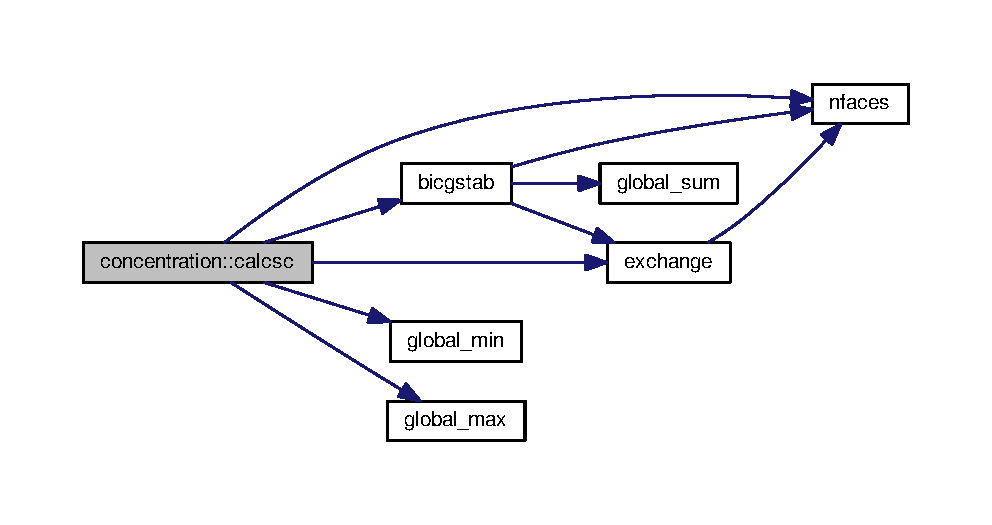
\includegraphics[width=350pt]{classconcentration_aeaccaf796f91761fea54318665fd2910_cgraph}
\end{center}
\end{figure}


\hypertarget{classconcentration_af2d433f438fa0b1f7ced09669de3f367}{\index{concentration@{concentration}!calculate\-\_\-concentration\-\_\-field@{calculate\-\_\-concentration\-\_\-field}}
\index{calculate\-\_\-concentration\-\_\-field@{calculate\-\_\-concentration\-\_\-field}!concentration@{concentration}}
\subsubsection[{calculate\-\_\-concentration\-\_\-field}]{\setlength{\rightskip}{0pt plus 5cm}subroutine, public concentration\-::calculate\-\_\-concentration\-\_\-field (
\begin{DoxyParamCaption}
{}
\end{DoxyParamCaption}
)}}\label{classconcentration_af2d433f438fa0b1f7ced09669de3f367}


Here is the call graph for this function\-:\nopagebreak
\begin{figure}[H]
\begin{center}
\leavevmode
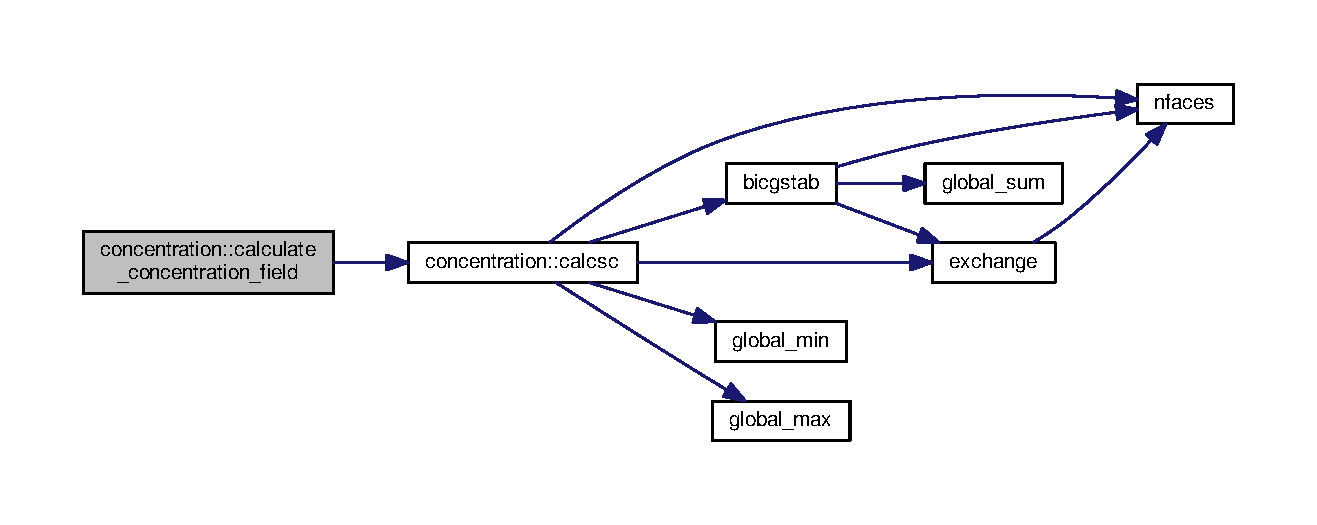
\includegraphics[width=350pt]{classconcentration_af2d433f438fa0b1f7ced09669de3f367_cgraph}
\end{center}
\end{figure}




\subsection{Member Data Documentation}
\hypertarget{classconcentration_ad256eb4a1ceeed0b362255ae96f0c04d}{\index{concentration@{concentration}!sigt@{sigt}}
\index{sigt@{sigt}!concentration@{concentration}}
\subsubsection[{sigt}]{\setlength{\rightskip}{0pt plus 5cm}real(dp), parameter concentration\-::sigt = 0.\-9\-\_\-dp}}\label{classconcentration_ad256eb4a1ceeed0b362255ae96f0c04d}


The documentation for this module was generated from the following file\-:\begin{DoxyCompactItemize}
\item 
src-\/par/\hyperlink{concentration_8f90}{concentration.\-f90}\end{DoxyCompactItemize}

\hypertarget{structsparse__matrix_1_1csrmatrix}{\section{sparse\-\_\-matrix\-:\-:csrmatrix Type Reference}
\label{structsparse__matrix_1_1csrmatrix}\index{sparse\-\_\-matrix\-::csrmatrix@{sparse\-\_\-matrix\-::csrmatrix}}
}
\subsection*{Public Attributes}
\begin{DoxyCompactItemize}
\item 
integer, dimension(\-:), allocatable \hyperlink{structsparse__matrix_1_1csrmatrix_a5eeedab30cbd4d8853974d1d123657af}{ioffset}
\item 
integer, dimension(\-:), allocatable \hyperlink{structsparse__matrix_1_1csrmatrix_aba7625ddfb8baff76458280c3060bcfc}{ja}
\item 
real(dp), dimension(\-:), allocatable \hyperlink{structsparse__matrix_1_1csrmatrix_a4d30e2bc5e35d70781f4626f39abbc6d}{coef}
\end{DoxyCompactItemize}


\subsection{Member Data Documentation}
\hypertarget{structsparse__matrix_1_1csrmatrix_a4d30e2bc5e35d70781f4626f39abbc6d}{\index{sparse\-\_\-matrix\-::csrmatrix@{sparse\-\_\-matrix\-::csrmatrix}!coef@{coef}}
\index{coef@{coef}!sparse_matrix::csrmatrix@{sparse\-\_\-matrix\-::csrmatrix}}
\subsubsection[{coef}]{\setlength{\rightskip}{0pt plus 5cm}real(dp), dimension(\-:), allocatable sparse\-\_\-matrix\-::csrmatrix\-::coef}}\label{structsparse__matrix_1_1csrmatrix_a4d30e2bc5e35d70781f4626f39abbc6d}
\hypertarget{structsparse__matrix_1_1csrmatrix_a5eeedab30cbd4d8853974d1d123657af}{\index{sparse\-\_\-matrix\-::csrmatrix@{sparse\-\_\-matrix\-::csrmatrix}!ioffset@{ioffset}}
\index{ioffset@{ioffset}!sparse_matrix::csrmatrix@{sparse\-\_\-matrix\-::csrmatrix}}
\subsubsection[{ioffset}]{\setlength{\rightskip}{0pt plus 5cm}integer, dimension(\-:), allocatable sparse\-\_\-matrix\-::csrmatrix\-::ioffset}}\label{structsparse__matrix_1_1csrmatrix_a5eeedab30cbd4d8853974d1d123657af}
\hypertarget{structsparse__matrix_1_1csrmatrix_aba7625ddfb8baff76458280c3060bcfc}{\index{sparse\-\_\-matrix\-::csrmatrix@{sparse\-\_\-matrix\-::csrmatrix}!ja@{ja}}
\index{ja@{ja}!sparse_matrix::csrmatrix@{sparse\-\_\-matrix\-::csrmatrix}}
\subsubsection[{ja}]{\setlength{\rightskip}{0pt plus 5cm}integer, dimension(\-:), allocatable sparse\-\_\-matrix\-::csrmatrix\-::ja}}\label{structsparse__matrix_1_1csrmatrix_aba7625ddfb8baff76458280c3060bcfc}


The documentation for this type was generated from the following file\-:\begin{DoxyCompactItemize}
\item 
src-\/par/\hyperlink{sparse__matrix_8f90}{sparse\-\_\-matrix.\-f90}\end{DoxyCompactItemize}

\hypertarget{classfaceflux__mass}{\section{faceflux\-\_\-mass Module Reference}
\label{classfaceflux__mass}\index{faceflux\-\_\-mass@{faceflux\-\_\-mass}}
}
\subsection*{Public Member Functions}
\begin{DoxyCompactItemize}
\item 
subroutine, public \hyperlink{classfaceflux__mass_adbb67f102fcdca57912e60bf8eaf75a4}{facefluxmass} (\hyperlink{CourantNo_8h_accea320a458bb8759c7ece360e05ddf4}{ijp}, ijn, xf, yf, zf, arx, ary, arz, lambda, cap, can, fluxmass)
\item 
subroutine, public \hyperlink{classfaceflux__mass_af0a6454f25b95c4c5586c8a25b31b073}{facefluxmass2} (\hyperlink{CourantNo_8h_accea320a458bb8759c7ece360e05ddf4}{ijp}, ijn, xf, yf, zf, arx, ary, arz, lambda, cap, can, fluxmass)
\item 
subroutine, public \hyperlink{classfaceflux__mass_ae73f110c08fa18ca7bb48808f22781a3}{facefluxmass\-\_\-piso} (\hyperlink{CourantNo_8h_accea320a458bb8759c7ece360e05ddf4}{ijp}, ijn, xf, yf, zf, arx, ary, arz, lambda, cap, can, flmass)
\item 
subroutine, public \hyperlink{classfaceflux__mass_a10e4d5e3230667bd512b3dbea8eba78b}{fluxmc} (\hyperlink{CourantNo_8h_accea320a458bb8759c7ece360e05ddf4}{ijp}, ijn, xf, yf, zf, arx, ary, arz, lambda, fmcor)
\end{DoxyCompactItemize}


\subsection{Member Function/\-Subroutine Documentation}
\hypertarget{classfaceflux__mass_adbb67f102fcdca57912e60bf8eaf75a4}{\index{faceflux\-\_\-mass@{faceflux\-\_\-mass}!facefluxmass@{facefluxmass}}
\index{facefluxmass@{facefluxmass}!faceflux_mass@{faceflux\-\_\-mass}}
\subsubsection[{facefluxmass}]{\setlength{\rightskip}{0pt plus 5cm}subroutine, public faceflux\-\_\-mass\-::facefluxmass (
\begin{DoxyParamCaption}
\item[{integer, intent(in)}]{ijp, }
\item[{integer, intent(in)}]{ijn, }
\item[{real(dp), intent(in)}]{xf, }
\item[{real(dp), intent(in)}]{yf, }
\item[{real(dp), intent(in)}]{zf, }
\item[{real(dp), intent(in)}]{arx, }
\item[{real(dp), intent(in)}]{ary, }
\item[{real(dp), intent(in)}]{arz, }
\item[{real(dp), intent(in)}]{lambda, }
\item[{real(dp), intent(inout)}]{cap, }
\item[{real(dp), intent(inout)}]{can, }
\item[{real(dp), intent(inout)}]{fluxmass}
\end{DoxyParamCaption}
)}}\label{classfaceflux__mass_adbb67f102fcdca57912e60bf8eaf75a4}


Here is the call graph for this function\-:\nopagebreak
\begin{figure}[H]
\begin{center}
\leavevmode
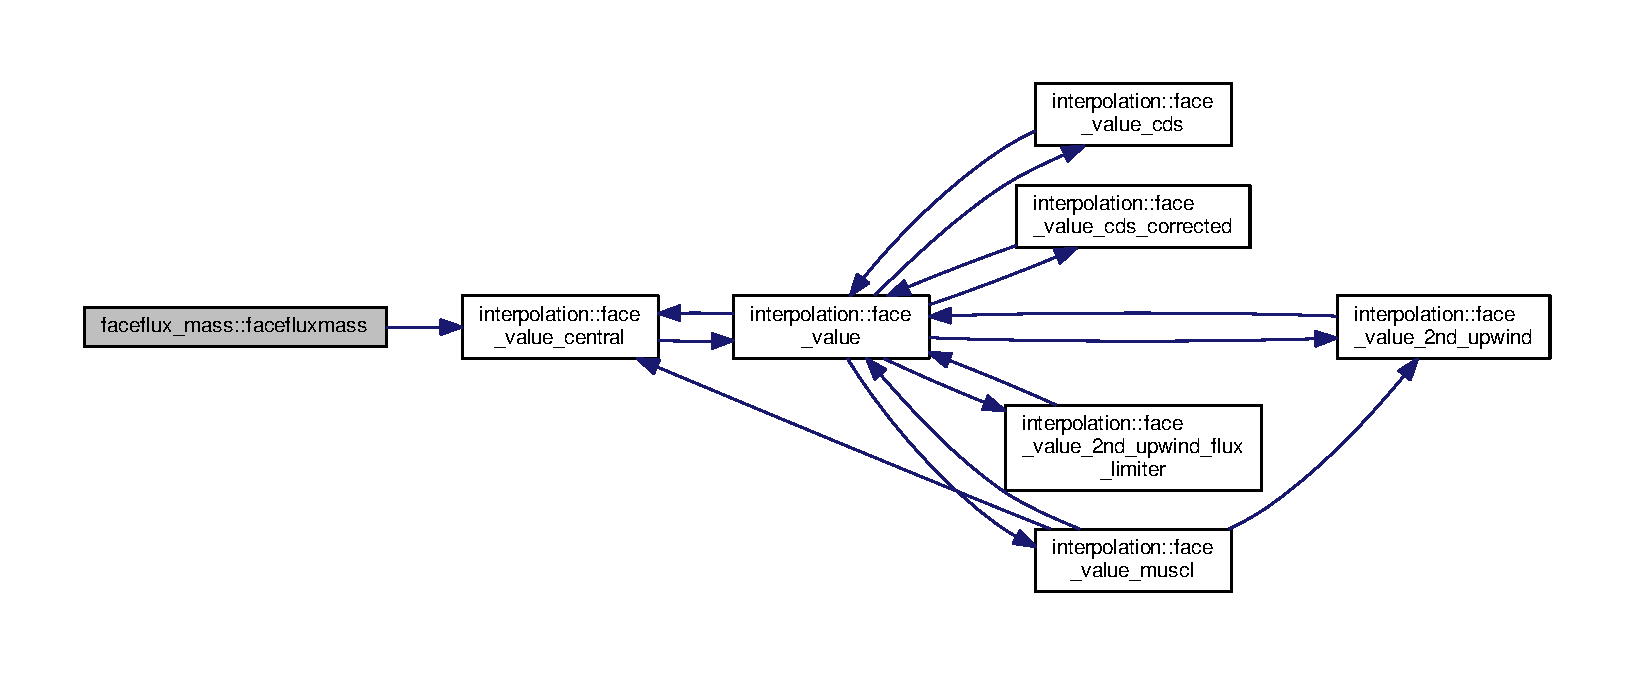
\includegraphics[width=350pt]{classfaceflux__mass_adbb67f102fcdca57912e60bf8eaf75a4_cgraph}
\end{center}
\end{figure}


\hypertarget{classfaceflux__mass_af0a6454f25b95c4c5586c8a25b31b073}{\index{faceflux\-\_\-mass@{faceflux\-\_\-mass}!facefluxmass2@{facefluxmass2}}
\index{facefluxmass2@{facefluxmass2}!faceflux_mass@{faceflux\-\_\-mass}}
\subsubsection[{facefluxmass2}]{\setlength{\rightskip}{0pt plus 5cm}subroutine, public faceflux\-\_\-mass\-::facefluxmass2 (
\begin{DoxyParamCaption}
\item[{integer, intent(in)}]{ijp, }
\item[{integer, intent(in)}]{ijn, }
\item[{real(dp), intent(in)}]{xf, }
\item[{real(dp), intent(in)}]{yf, }
\item[{real(dp), intent(in)}]{zf, }
\item[{real(dp), intent(in)}]{arx, }
\item[{real(dp), intent(in)}]{ary, }
\item[{real(dp), intent(in)}]{arz, }
\item[{real(dp), intent(in)}]{lambda, }
\item[{real(dp), intent(inout)}]{cap, }
\item[{real(dp), intent(inout)}]{can, }
\item[{real(dp), intent(inout)}]{fluxmass}
\end{DoxyParamCaption}
)}}\label{classfaceflux__mass_af0a6454f25b95c4c5586c8a25b31b073}


Here is the call graph for this function\-:\nopagebreak
\begin{figure}[H]
\begin{center}
\leavevmode
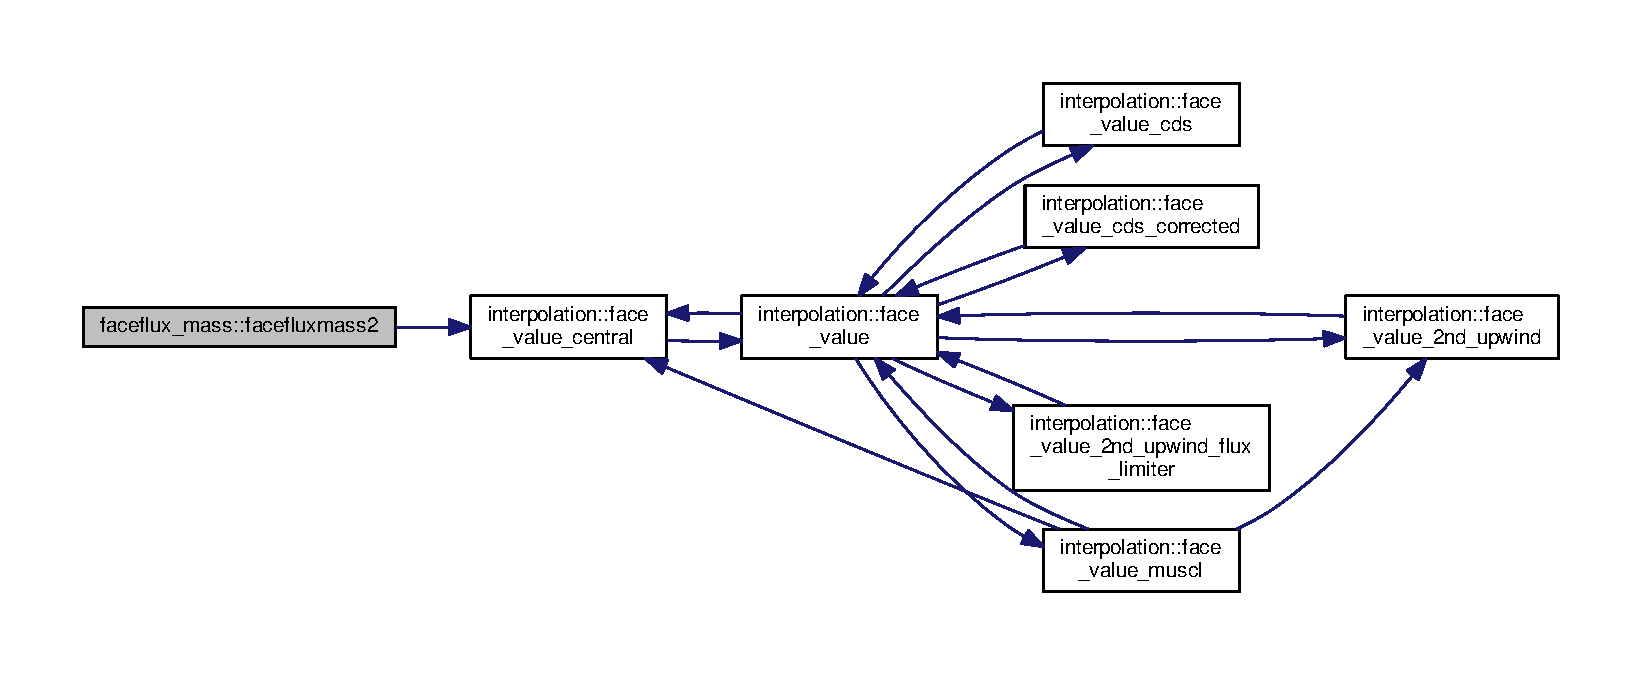
\includegraphics[width=350pt]{classfaceflux__mass_af0a6454f25b95c4c5586c8a25b31b073_cgraph}
\end{center}
\end{figure}


\hypertarget{classfaceflux__mass_ae73f110c08fa18ca7bb48808f22781a3}{\index{faceflux\-\_\-mass@{faceflux\-\_\-mass}!facefluxmass\-\_\-piso@{facefluxmass\-\_\-piso}}
\index{facefluxmass\-\_\-piso@{facefluxmass\-\_\-piso}!faceflux_mass@{faceflux\-\_\-mass}}
\subsubsection[{facefluxmass\-\_\-piso}]{\setlength{\rightskip}{0pt plus 5cm}subroutine, public faceflux\-\_\-mass\-::facefluxmass\-\_\-piso (
\begin{DoxyParamCaption}
\item[{integer, intent(in)}]{ijp, }
\item[{integer, intent(in)}]{ijn, }
\item[{real(dp), intent(in)}]{xf, }
\item[{real(dp), intent(in)}]{yf, }
\item[{real(dp), intent(in)}]{zf, }
\item[{real(dp), intent(in)}]{arx, }
\item[{real(dp), intent(in)}]{ary, }
\item[{real(dp), intent(in)}]{arz, }
\item[{real(dp), intent(in)}]{lambda, }
\item[{real(dp), intent(inout)}]{cap, }
\item[{real(dp), intent(inout)}]{can, }
\item[{real(dp), intent(inout)}]{flmass}
\end{DoxyParamCaption}
)}}\label{classfaceflux__mass_ae73f110c08fa18ca7bb48808f22781a3}


Here is the call graph for this function\-:\nopagebreak
\begin{figure}[H]
\begin{center}
\leavevmode
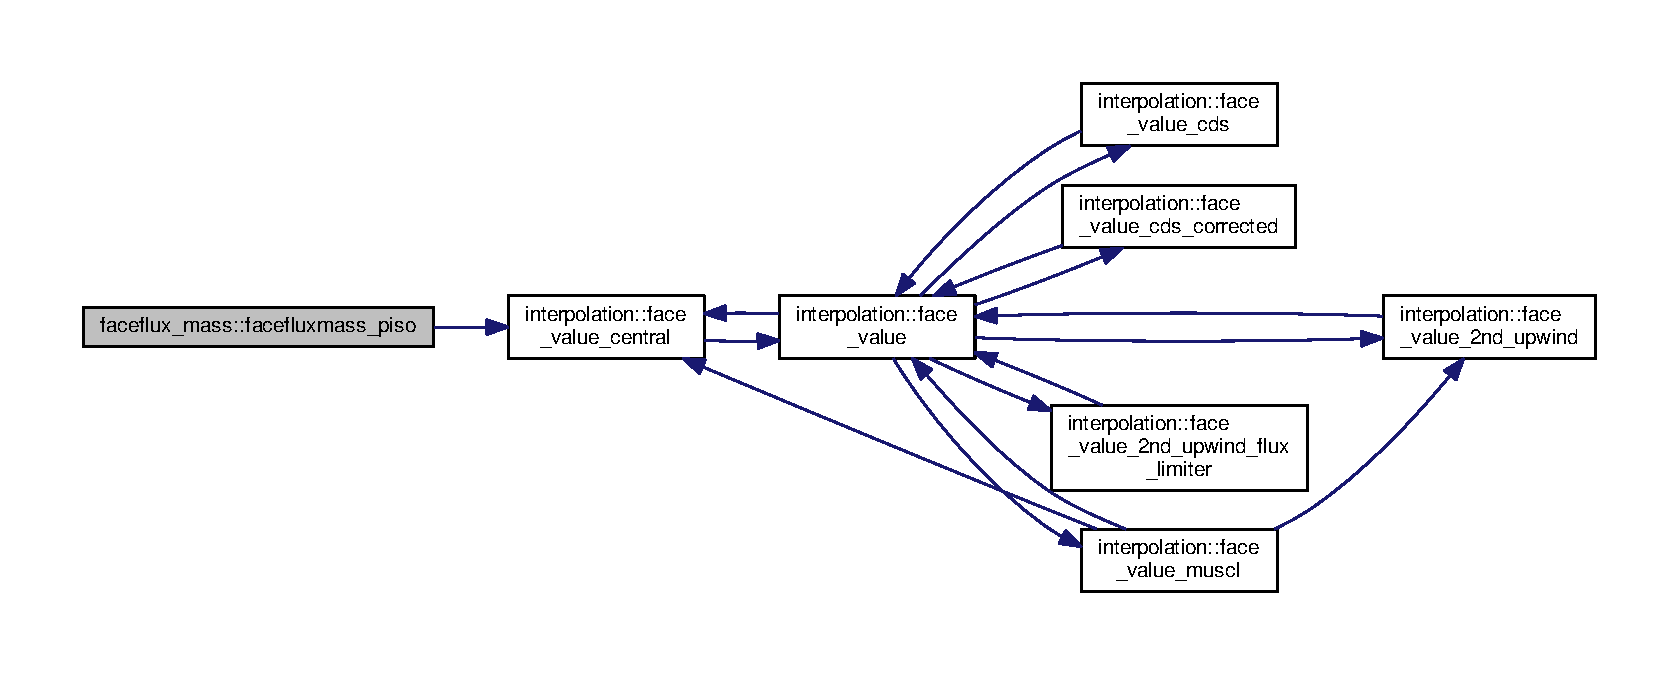
\includegraphics[width=350pt]{classfaceflux__mass_ae73f110c08fa18ca7bb48808f22781a3_cgraph}
\end{center}
\end{figure}


\hypertarget{classfaceflux__mass_a10e4d5e3230667bd512b3dbea8eba78b}{\index{faceflux\-\_\-mass@{faceflux\-\_\-mass}!fluxmc@{fluxmc}}
\index{fluxmc@{fluxmc}!faceflux_mass@{faceflux\-\_\-mass}}
\subsubsection[{fluxmc}]{\setlength{\rightskip}{0pt plus 5cm}subroutine, public faceflux\-\_\-mass\-::fluxmc (
\begin{DoxyParamCaption}
\item[{integer, intent(in)}]{ijp, }
\item[{integer, intent(in)}]{ijn, }
\item[{real(dp), intent(in)}]{xf, }
\item[{real(dp), intent(in)}]{yf, }
\item[{real(dp), intent(in)}]{zf, }
\item[{real(dp), intent(in)}]{arx, }
\item[{real(dp), intent(in)}]{ary, }
\item[{real(dp), intent(in)}]{arz, }
\item[{real(dp), intent(in)}]{lambda, }
\item[{real(dp), intent(inout)}]{fmcor}
\end{DoxyParamCaption}
)}}\label{classfaceflux__mass_a10e4d5e3230667bd512b3dbea8eba78b}


The documentation for this module was generated from the following file\-:\begin{DoxyCompactItemize}
\item 
src-\/par/\hyperlink{facefluxmass_8f90}{facefluxmass.\-f90}\end{DoxyCompactItemize}

\hypertarget{classfaceflux__velocity}{\section{faceflux\-\_\-velocity Module Reference}
\label{classfaceflux__velocity}\index{faceflux\-\_\-velocity@{faceflux\-\_\-velocity}}
}
\subsection*{Data Types}
\begin{DoxyCompactItemize}
\item 
interface \hyperlink{interfacefaceflux__velocity_1_1facefluxuvw}{facefluxuvw}
\end{DoxyCompactItemize}
\subsection*{Public Member Functions}
\begin{DoxyCompactItemize}
\item 
subroutine, public \hyperlink{classfaceflux__velocity_ae05a209571d2c349b0ecd18c8476dfad}{facefluxuvw} (\hyperlink{CourantNo_8h_accea320a458bb8759c7ece360e05ddf4}{ijp}, ijn, xf, yf, zf, arx, ary, arz, flomass, lambda, gam, cap, can, sup, svp, swp)
\end{DoxyCompactItemize}
\subsection*{Private Member Functions}
\begin{DoxyCompactItemize}
\item 
subroutine \hyperlink{classfaceflux__velocity_a1a47191b7f9978400d8b19fac879aec6}{facefluxuvw\-\_\-boundary} (\hyperlink{CourantNo_8h_accea320a458bb8759c7ece360e05ddf4}{ijp}, ijb, xf, yf, zf, arx, ary, arz, flomass, cap, can, sup, svp, swp)
\end{DoxyCompactItemize}


\subsection{Member Function/\-Subroutine Documentation}
\hypertarget{classfaceflux__velocity_ae05a209571d2c349b0ecd18c8476dfad}{\index{faceflux\-\_\-velocity@{faceflux\-\_\-velocity}!facefluxuvw@{facefluxuvw}}
\index{facefluxuvw@{facefluxuvw}!faceflux_velocity@{faceflux\-\_\-velocity}}
\subsubsection[{facefluxuvw}]{\setlength{\rightskip}{0pt plus 5cm}subroutine, public {\bf faceflux\-\_\-velocity\-::facefluxuvw} (
\begin{DoxyParamCaption}
\item[{integer, intent(in)}]{ijp, }
\item[{integer, intent(in)}]{ijn, }
\item[{real(dp), intent(in)}]{xf, }
\item[{real(dp), intent(in)}]{yf, }
\item[{real(dp), intent(in)}]{zf, }
\item[{real(dp), intent(in)}]{arx, }
\item[{real(dp), intent(in)}]{ary, }
\item[{real(dp), intent(in)}]{arz, }
\item[{real(dp), intent(in)}]{flomass, }
\item[{real(dp), intent(in)}]{lambda, }
\item[{real(dp), intent(in)}]{gam, }
\item[{real(dp), intent(inout)}]{cap, }
\item[{real(dp), intent(inout)}]{can, }
\item[{real(dp), intent(inout)}]{sup, }
\item[{real(dp), intent(inout)}]{svp, }
\item[{real(dp), intent(inout)}]{swp}
\end{DoxyParamCaption}
)}}\label{classfaceflux__velocity_ae05a209571d2c349b0ecd18c8476dfad}


Here is the call graph for this function\-:\nopagebreak
\begin{figure}[H]
\begin{center}
\leavevmode
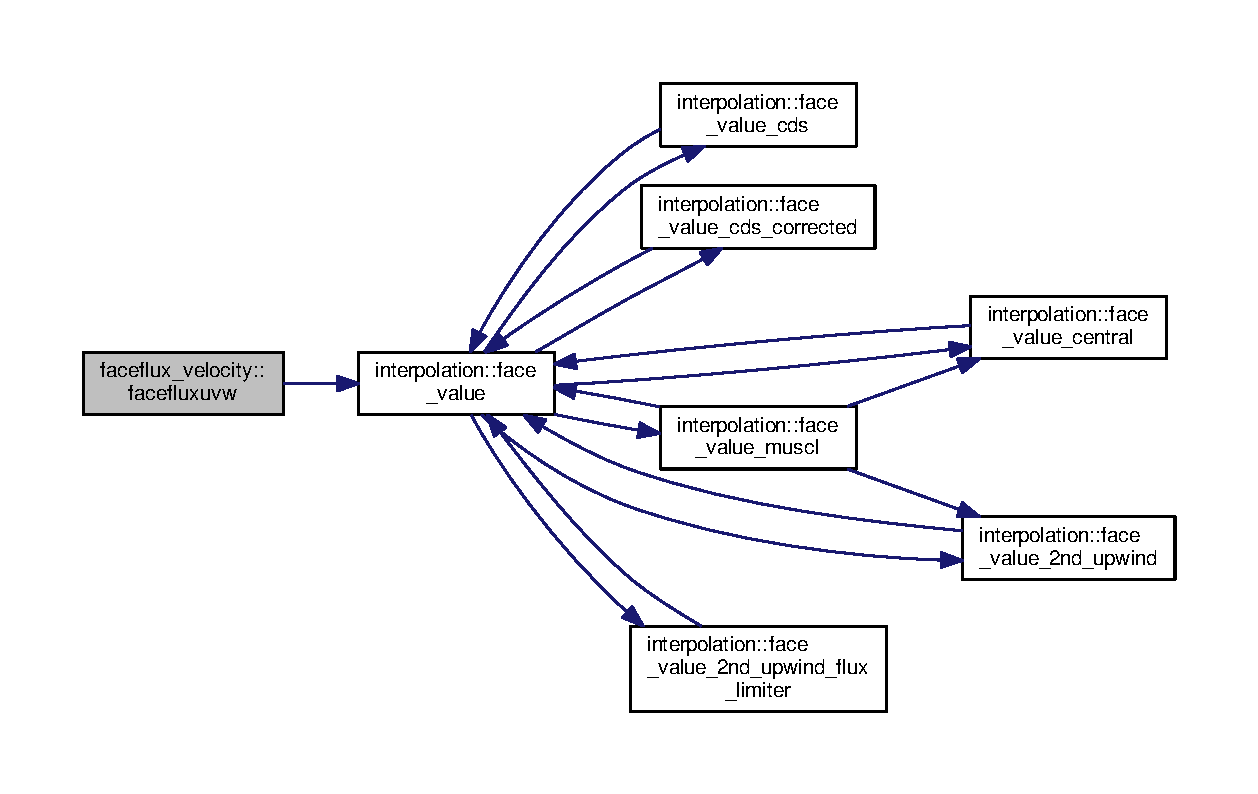
\includegraphics[width=350pt]{classfaceflux__velocity_ae05a209571d2c349b0ecd18c8476dfad_cgraph}
\end{center}
\end{figure}


\hypertarget{classfaceflux__velocity_a1a47191b7f9978400d8b19fac879aec6}{\index{faceflux\-\_\-velocity@{faceflux\-\_\-velocity}!facefluxuvw\-\_\-boundary@{facefluxuvw\-\_\-boundary}}
\index{facefluxuvw\-\_\-boundary@{facefluxuvw\-\_\-boundary}!faceflux_velocity@{faceflux\-\_\-velocity}}
\subsubsection[{facefluxuvw\-\_\-boundary}]{\setlength{\rightskip}{0pt plus 5cm}subroutine faceflux\-\_\-velocity\-::facefluxuvw\-\_\-boundary (
\begin{DoxyParamCaption}
\item[{integer, intent(in)}]{ijp, }
\item[{integer, intent(in)}]{ijb, }
\item[{real(dp), intent(in)}]{xf, }
\item[{real(dp), intent(in)}]{yf, }
\item[{real(dp), intent(in)}]{zf, }
\item[{real(dp), intent(in)}]{arx, }
\item[{real(dp), intent(in)}]{ary, }
\item[{real(dp), intent(in)}]{arz, }
\item[{real(dp), intent(in)}]{flomass, }
\item[{real(dp), intent(inout)}]{cap, }
\item[{real(dp), intent(inout)}]{can, }
\item[{real(dp), intent(inout)}]{sup, }
\item[{real(dp), intent(inout)}]{svp, }
\item[{real(dp), intent(inout)}]{swp}
\end{DoxyParamCaption}
)\hspace{0.3cm}{\ttfamily [private]}}}\label{classfaceflux__velocity_a1a47191b7f9978400d8b19fac879aec6}


The documentation for this module was generated from the following file\-:\begin{DoxyCompactItemize}
\item 
src-\/par/\hyperlink{faceflux__velocity_8f90}{faceflux\-\_\-velocity.\-f90}\end{DoxyCompactItemize}

\hypertarget{interfacescalar__fluxes_1_1facefluxsc}{\section{scalar\-\_\-fluxes\-:\-:facefluxsc Interface Reference}
\label{interfacescalar__fluxes_1_1facefluxsc}\index{scalar\-\_\-fluxes\-::facefluxsc@{scalar\-\_\-fluxes\-::facefluxsc}}
}
\subsection*{Public Member Functions}
\begin{DoxyCompactItemize}
\item 
subroutine \hyperlink{interfacescalar__fluxes_1_1facefluxsc_a68abc0ee379e9a19d00b339599a23c4b}{facefluxsc} (\hyperlink{CourantNo_8h_accea320a458bb8759c7ece360e05ddf4}{ijp}, ijn, xf, yf, zf, arx, ary, arz, flmass, lambda, gam, F\-I, d\-Fidxi, prtr, cap, can, suadd)
\item 
subroutine \hyperlink{interfacescalar__fluxes_1_1facefluxsc_a17ea978f35e3708c8c597b8ffab1df52}{facefluxsc\-\_\-nonconst\-\_\-prtr} (\hyperlink{CourantNo_8h_accea320a458bb8759c7ece360e05ddf4}{ijp}, ijn, xf, yf, zf, arx, ary, arz, flmass, lambda, gam, F\-I, d\-Fidxi, prtr\-\_\-ijp, prtr\-\_\-ijn, cap, can, suadd)
\item 
subroutine \hyperlink{interfacescalar__fluxes_1_1facefluxsc_ae48b1d123dcd71824c9d740bf2e08ccd}{facefluxsc\-\_\-boundary} (\hyperlink{CourantNo_8h_accea320a458bb8759c7ece360e05ddf4}{ijp}, ijn, xf, yf, zf, arx, ary, arz, flmass, F\-I, d\-Fidxi, prtr, cap, can, suadd)
\end{DoxyCompactItemize}


\subsection{Constructor \& Destructor Documentation}
\hypertarget{interfacescalar__fluxes_1_1facefluxsc_a68abc0ee379e9a19d00b339599a23c4b}{\index{scalar\-\_\-fluxes\-::facefluxsc@{scalar\-\_\-fluxes\-::facefluxsc}!facefluxsc@{facefluxsc}}
\index{facefluxsc@{facefluxsc}!scalar_fluxes::facefluxsc@{scalar\-\_\-fluxes\-::facefluxsc}}
\subsubsection[{facefluxsc}]{\setlength{\rightskip}{0pt plus 5cm}subroutine scalar\-\_\-fluxes\-::facefluxsc\-::facefluxsc (
\begin{DoxyParamCaption}
\item[{integer, intent(in)}]{ijp, }
\item[{integer, intent(in)}]{ijn, }
\item[{real(dp), intent(in)}]{xf, }
\item[{real(dp), intent(in)}]{yf, }
\item[{real(dp), intent(in)}]{zf, }
\item[{real(dp), intent(in)}]{arx, }
\item[{real(dp), intent(in)}]{ary, }
\item[{real(dp), intent(in)}]{arz, }
\item[{real(dp), intent(in)}]{flmass, }
\item[{real(dp), intent(in)}]{lambda, }
\item[{real(dp), intent(in)}]{gam, }
\item[{real(dp), dimension(numtotal), intent(in)}]{F\-I, }
\item[{real(dp), dimension(3,numcells), intent(in)}]{d\-Fidxi, }
\item[{real(dp), intent(in)}]{prtr, }
\item[{real(dp), intent(inout)}]{cap, }
\item[{real(dp), intent(inout)}]{can, }
\item[{real(dp), intent(inout)}]{suadd}
\end{DoxyParamCaption}
)}}\label{interfacescalar__fluxes_1_1facefluxsc_a68abc0ee379e9a19d00b339599a23c4b}


\subsection{Member Function/\-Subroutine Documentation}
\hypertarget{interfacescalar__fluxes_1_1facefluxsc_ae48b1d123dcd71824c9d740bf2e08ccd}{\index{scalar\-\_\-fluxes\-::facefluxsc@{scalar\-\_\-fluxes\-::facefluxsc}!facefluxsc\-\_\-boundary@{facefluxsc\-\_\-boundary}}
\index{facefluxsc\-\_\-boundary@{facefluxsc\-\_\-boundary}!scalar_fluxes::facefluxsc@{scalar\-\_\-fluxes\-::facefluxsc}}
\subsubsection[{facefluxsc\-\_\-boundary}]{\setlength{\rightskip}{0pt plus 5cm}subroutine scalar\-\_\-fluxes\-::facefluxsc\-::facefluxsc\-\_\-boundary (
\begin{DoxyParamCaption}
\item[{integer, intent(in)}]{ijp, }
\item[{integer, intent(in)}]{ijn, }
\item[{real(dp), intent(in)}]{xf, }
\item[{real(dp), intent(in)}]{yf, }
\item[{real(dp), intent(in)}]{zf, }
\item[{real(dp), intent(in)}]{arx, }
\item[{real(dp), intent(in)}]{ary, }
\item[{real(dp), intent(in)}]{arz, }
\item[{real(dp), intent(in)}]{flmass, }
\item[{real(dp), dimension(numtotal), intent(in)}]{F\-I, }
\item[{real(dp), dimension(3,numtotal), intent(in)}]{d\-Fidxi, }
\item[{real(dp), intent(in)}]{prtr, }
\item[{real(dp), intent(inout)}]{cap, }
\item[{real(dp), intent(inout)}]{can, }
\item[{real(dp), intent(inout)}]{suadd}
\end{DoxyParamCaption}
)}}\label{interfacescalar__fluxes_1_1facefluxsc_ae48b1d123dcd71824c9d740bf2e08ccd}
\hypertarget{interfacescalar__fluxes_1_1facefluxsc_a17ea978f35e3708c8c597b8ffab1df52}{\index{scalar\-\_\-fluxes\-::facefluxsc@{scalar\-\_\-fluxes\-::facefluxsc}!facefluxsc\-\_\-nonconst\-\_\-prtr@{facefluxsc\-\_\-nonconst\-\_\-prtr}}
\index{facefluxsc\-\_\-nonconst\-\_\-prtr@{facefluxsc\-\_\-nonconst\-\_\-prtr}!scalar_fluxes::facefluxsc@{scalar\-\_\-fluxes\-::facefluxsc}}
\subsubsection[{facefluxsc\-\_\-nonconst\-\_\-prtr}]{\setlength{\rightskip}{0pt plus 5cm}subroutine scalar\-\_\-fluxes\-::facefluxsc\-::facefluxsc\-\_\-nonconst\-\_\-prtr (
\begin{DoxyParamCaption}
\item[{integer, intent(in)}]{ijp, }
\item[{integer, intent(in)}]{ijn, }
\item[{real(dp), intent(in)}]{xf, }
\item[{real(dp), intent(in)}]{yf, }
\item[{real(dp), intent(in)}]{zf, }
\item[{real(dp), intent(in)}]{arx, }
\item[{real(dp), intent(in)}]{ary, }
\item[{real(dp), intent(in)}]{arz, }
\item[{real(dp), intent(in)}]{flmass, }
\item[{real(dp), intent(in)}]{lambda, }
\item[{real(dp), intent(in)}]{gam, }
\item[{real(dp), dimension(numtotal), intent(in)}]{F\-I, }
\item[{real(dp), dimension(3,numcells), intent(in)}]{d\-Fidxi, }
\item[{real(dp), intent(in)}]{prtr\-\_\-ijp, }
\item[{real(dp), intent(in)}]{prtr\-\_\-ijn, }
\item[{real(dp), intent(inout)}]{cap, }
\item[{real(dp), intent(inout)}]{can, }
\item[{real(dp), intent(inout)}]{suadd}
\end{DoxyParamCaption}
)}}\label{interfacescalar__fluxes_1_1facefluxsc_a17ea978f35e3708c8c597b8ffab1df52}


The documentation for this interface was generated from the following file\-:\begin{DoxyCompactItemize}
\item 
src-\/par/\hyperlink{scalar__fluxes_8f90}{scalar\-\_\-fluxes.\-f90}\end{DoxyCompactItemize}

\hypertarget{interfacefaceflux__velocity_1_1facefluxuvw}{}\doxysection{faceflux\+\_\+velocity\+::facefluxuvw Interface Reference}
\label{interfacefaceflux__velocity_1_1facefluxuvw}\index{faceflux\_velocity::facefluxuvw@{faceflux\_velocity::facefluxuvw}}
\doxysubsection*{Public Member Functions}
\begin{DoxyCompactItemize}
\item 
subroutine \mbox{\hyperlink{interfacefaceflux__velocity_1_1facefluxuvw_ada009356e8199a1f363a431e40068e45}{facefluxuvw}} (ijp, ijn, xf, yf, zf, arx, ary, arz, flomass, lambda, gam, cap, can, sup, svp, swp)
\item 
subroutine \mbox{\hyperlink{interfacefaceflux__velocity_1_1facefluxuvw_abe1dbe2c4c152287906de80992d26fa1}{facefluxuvw\+\_\+boundary}} (ijp, ijb, xf, yf, zf, arx, ary, arz, flomass, cap, can, sup, svp, swp)
\end{DoxyCompactItemize}


\doxysubsection{Constructor \& Destructor Documentation}
\mbox{\Hypertarget{interfacefaceflux__velocity_1_1facefluxuvw_ada009356e8199a1f363a431e40068e45}\label{interfacefaceflux__velocity_1_1facefluxuvw_ada009356e8199a1f363a431e40068e45}} 
\index{faceflux\_velocity::facefluxuvw@{faceflux\_velocity::facefluxuvw}!facefluxuvw@{facefluxuvw}}
\index{facefluxuvw@{facefluxuvw}!faceflux\_velocity::facefluxuvw@{faceflux\_velocity::facefluxuvw}}
\doxysubsubsection{\texorpdfstring{facefluxuvw()}{facefluxuvw()}}
{\footnotesize\ttfamily subroutine faceflux\+\_\+velocity\+::facefluxuvw\+::facefluxuvw (\begin{DoxyParamCaption}\item[{integer, intent(in)}]{ijp,  }\item[{integer, intent(in)}]{ijn,  }\item[{real(dp), intent(in)}]{xf,  }\item[{real(dp), intent(in)}]{yf,  }\item[{real(dp), intent(in)}]{zf,  }\item[{real(dp), intent(in)}]{arx,  }\item[{real(dp), intent(in)}]{ary,  }\item[{real(dp), intent(in)}]{arz,  }\item[{real(dp), intent(in)}]{flomass,  }\item[{real(dp), intent(in)}]{lambda,  }\item[{real(dp), intent(in)}]{gam,  }\item[{real(dp), intent(inout)}]{cap,  }\item[{real(dp), intent(inout)}]{can,  }\item[{real(dp), intent(inout)}]{sup,  }\item[{real(dp), intent(inout)}]{svp,  }\item[{real(dp), intent(inout)}]{swp }\end{DoxyParamCaption})}



\doxysubsection{Member Function/\+Subroutine Documentation}
\mbox{\Hypertarget{interfacefaceflux__velocity_1_1facefluxuvw_abe1dbe2c4c152287906de80992d26fa1}\label{interfacefaceflux__velocity_1_1facefluxuvw_abe1dbe2c4c152287906de80992d26fa1}} 
\index{faceflux\_velocity::facefluxuvw@{faceflux\_velocity::facefluxuvw}!facefluxuvw\_boundary@{facefluxuvw\_boundary}}
\index{facefluxuvw\_boundary@{facefluxuvw\_boundary}!faceflux\_velocity::facefluxuvw@{faceflux\_velocity::facefluxuvw}}
\doxysubsubsection{\texorpdfstring{facefluxuvw\_boundary()}{facefluxuvw\_boundary()}}
{\footnotesize\ttfamily subroutine faceflux\+\_\+velocity\+::facefluxuvw\+::facefluxuvw\+\_\+boundary (\begin{DoxyParamCaption}\item[{integer, intent(in)}]{ijp,  }\item[{integer, intent(in)}]{ijb,  }\item[{real(dp), intent(in)}]{xf,  }\item[{real(dp), intent(in)}]{yf,  }\item[{real(dp), intent(in)}]{zf,  }\item[{real(dp), intent(in)}]{arx,  }\item[{real(dp), intent(in)}]{ary,  }\item[{real(dp), intent(in)}]{arz,  }\item[{real(dp), intent(in)}]{flomass,  }\item[{real(dp), intent(inout)}]{cap,  }\item[{real(dp), intent(inout)}]{can,  }\item[{real(dp), intent(inout)}]{sup,  }\item[{real(dp), intent(inout)}]{svp,  }\item[{real(dp), intent(inout)}]{swp }\end{DoxyParamCaption})}



The documentation for this interface was generated from the following file\+:\begin{DoxyCompactItemize}
\item 
src-\/par/\mbox{\hyperlink{faceflux__velocity_8f90}{faceflux\+\_\+velocity.\+f90}}\end{DoxyCompactItemize}

\hypertarget{classfield__initialization}{\section{field\-\_\-initialization Module Reference}
\label{classfield__initialization}\index{field\-\_\-initialization@{field\-\_\-initialization}}
}
\subsection*{Public Member Functions}
\begin{DoxyCompactItemize}
\item 
subroutine \hyperlink{classfield__initialization_a48dbf36aa2ebe47dd8750abf2fea62e6}{initialize\-\_\-vector\-\_\-field} (u, v, w, d\-Udxi, field\-\_\-name)
\item 
subroutine \hyperlink{classfield__initialization_a20b45b7838e83793d92fd20176bdf1c6}{initialize\-\_\-scalar\-\_\-field} (T, d\-Tdxi, field\-\_\-name)
\end{DoxyCompactItemize}


\subsection{Member Function/\-Subroutine Documentation}
\hypertarget{classfield__initialization_a20b45b7838e83793d92fd20176bdf1c6}{\index{field\-\_\-initialization@{field\-\_\-initialization}!initialize\-\_\-scalar\-\_\-field@{initialize\-\_\-scalar\-\_\-field}}
\index{initialize\-\_\-scalar\-\_\-field@{initialize\-\_\-scalar\-\_\-field}!field_initialization@{field\-\_\-initialization}}
\subsubsection[{initialize\-\_\-scalar\-\_\-field}]{\setlength{\rightskip}{0pt plus 5cm}subroutine field\-\_\-initialization\-::initialize\-\_\-scalar\-\_\-field (
\begin{DoxyParamCaption}
\item[{real(dp), dimension(numtotal)}]{T, }
\item[{real(dp), dimension(numtotal)}]{d\-Tdxi, }
\item[{character(len=$\ast$)}]{field\-\_\-name}
\end{DoxyParamCaption}
)}}\label{classfield__initialization_a20b45b7838e83793d92fd20176bdf1c6}


Here is the call graph for this function\-:\nopagebreak
\begin{figure}[H]
\begin{center}
\leavevmode
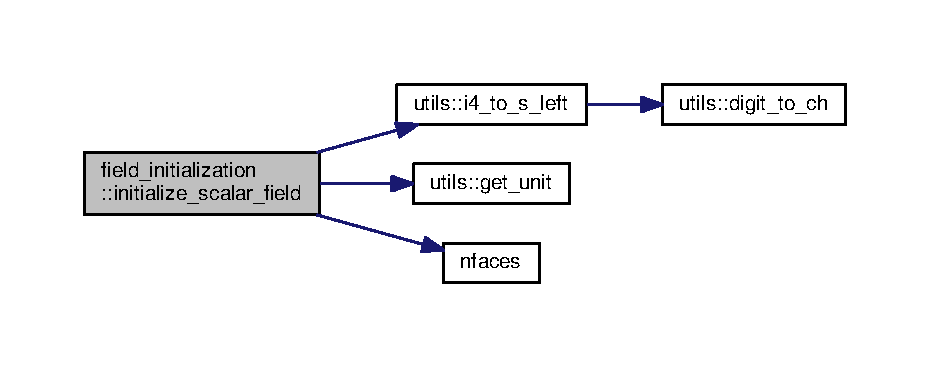
\includegraphics[width=350pt]{classfield__initialization_a20b45b7838e83793d92fd20176bdf1c6_cgraph}
\end{center}
\end{figure}


\hypertarget{classfield__initialization_a48dbf36aa2ebe47dd8750abf2fea62e6}{\index{field\-\_\-initialization@{field\-\_\-initialization}!initialize\-\_\-vector\-\_\-field@{initialize\-\_\-vector\-\_\-field}}
\index{initialize\-\_\-vector\-\_\-field@{initialize\-\_\-vector\-\_\-field}!field_initialization@{field\-\_\-initialization}}
\subsubsection[{initialize\-\_\-vector\-\_\-field}]{\setlength{\rightskip}{0pt plus 5cm}subroutine field\-\_\-initialization\-::initialize\-\_\-vector\-\_\-field (
\begin{DoxyParamCaption}
\item[{real(dp), dimension(numtotal)}]{u, }
\item[{real(dp), dimension(numtotal)}]{v, }
\item[{real(dp), dimension(numtotal)}]{w, }
\item[{real(dp), dimension(3,numtotal)}]{d\-Udxi, }
\item[{character(len=$\ast$)}]{field\-\_\-name}
\end{DoxyParamCaption}
)}}\label{classfield__initialization_a48dbf36aa2ebe47dd8750abf2fea62e6}


Here is the call graph for this function\-:\nopagebreak
\begin{figure}[H]
\begin{center}
\leavevmode
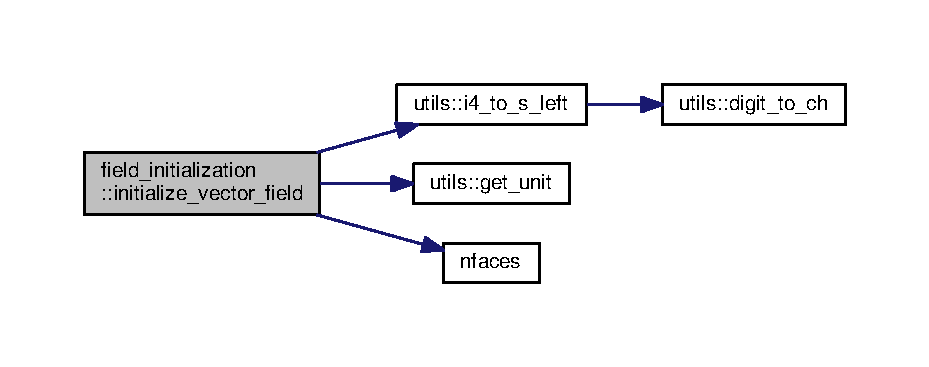
\includegraphics[width=350pt]{classfield__initialization_a48dbf36aa2ebe47dd8750abf2fea62e6_cgraph}
\end{center}
\end{figure}




The documentation for this module was generated from the following file\-:\begin{DoxyCompactItemize}
\item 
src-\/par/\hyperlink{field__initialization_8f90}{field\-\_\-initialization.\-f90}\end{DoxyCompactItemize}

\hypertarget{classfieldmanipulation}{\section{fieldmanipulation Module Reference}
\label{classfieldmanipulation}\index{fieldmanipulation@{fieldmanipulation}}
}
\subsection*{Public Member Functions}
\begin{DoxyCompactItemize}
\item 
real(dp) function \hyperlink{classfieldmanipulation_a0bdf9e1dcd8cee01d2a1f90bb96a1583}{volumeweightedaverage} (U)
\item 
subroutine \hyperlink{classfieldmanipulation_ad3594b987621ee1b66dc23373cba6482}{calcpressdiv}
\item 
real(dp) function, dimension(numcells) \hyperlink{classfieldmanipulation_aa58beed06659b15ede41acc5c6249991}{expldiv} (u)
\item 
subroutine \hyperlink{classfieldmanipulation_a8fa4949333251cce2f68dd0566a71e7b}{presfacedivinner} (\hyperlink{CourantNo_8h_accea320a458bb8759c7ece360e05ddf4}{ijp}, ijn, xfc, yfc, zfc, sx, sy, sz, fif, fi, df, dfxe, dfye, dfze)
\item 
subroutine \hyperlink{classfieldmanipulation_afbd4007fedcd5c8960dfc4a3905349a9}{facedivinner} (\hyperlink{CourantNo_8h_accea320a458bb8759c7ece360e05ddf4}{ijp}, ijn, xfc, yfc, zfc, sx, sy, sz, fif, fi, df, dfxe)
\item 
subroutine \hyperlink{classfieldmanipulation_aa28be3da5dcf8b277c6c28391f01a06e}{facedivboundary} (sx, sy, sz, fi, dfx)
\item 
subroutine \hyperlink{classfieldmanipulation_afe436887e04bd6717076c2bee1210f19}{presfacedivboundary} (sx, sy, sz, fi, dfx, dfy, dfz)
\item 
real(dp) function, dimension(numcells) \hyperlink{classfieldmanipulation_a8527c697c24116df3c60fce525a2c364}{average} (u)
\item 
real(dp) function, dimension(numfaces) \hyperlink{classfieldmanipulation_abe2f38fcc53d73b51061465e3cf9e3dd}{interpolate} (u)
\item 
real(dp) function, dimension(numcells) \hyperlink{classfieldmanipulation_a3f3fb8bda2659dd1f034ef8c5a99b405}{surfacesum} (u)
\item 
real(dp) function, dimension(numcells) \hyperlink{classfieldmanipulation_a3212f37b15b79464ad49e662e2a5a394}{surfaceintegrate} (u)
\item 
subroutine \hyperlink{classfieldmanipulation_aba8cce868dfdd1d679c48022ed786ea8}{faceinterpolatecdscorr} (\hyperlink{CourantNo_8h_accea320a458bb8759c7ece360e05ddf4}{ijp}, ijn, xfc, yfc, zfc, fif, fi, df, fie)
\item 
subroutine \hyperlink{classfieldmanipulation_a3e8ca2ca22fb46938f8a479a82c90205}{add\-\_\-random\-\_\-noise\-\_\-to\-\_\-field} (Phi, percent)
\end{DoxyCompactItemize}


\subsection{Member Function/\-Subroutine Documentation}
\hypertarget{classfieldmanipulation_a3e8ca2ca22fb46938f8a479a82c90205}{\index{fieldmanipulation@{fieldmanipulation}!add\-\_\-random\-\_\-noise\-\_\-to\-\_\-field@{add\-\_\-random\-\_\-noise\-\_\-to\-\_\-field}}
\index{add\-\_\-random\-\_\-noise\-\_\-to\-\_\-field@{add\-\_\-random\-\_\-noise\-\_\-to\-\_\-field}!fieldmanipulation@{fieldmanipulation}}
\subsubsection[{add\-\_\-random\-\_\-noise\-\_\-to\-\_\-field}]{\setlength{\rightskip}{0pt plus 5cm}subroutine fieldmanipulation\-::add\-\_\-random\-\_\-noise\-\_\-to\-\_\-field (
\begin{DoxyParamCaption}
\item[{real(dp), dimension(numtotal), intent(inout)}]{Phi, }
\item[{integer, intent(in)}]{percent}
\end{DoxyParamCaption}
)}}\label{classfieldmanipulation_a3e8ca2ca22fb46938f8a479a82c90205}


Here is the call graph for this function\-:\nopagebreak
\begin{figure}[H]
\begin{center}
\leavevmode
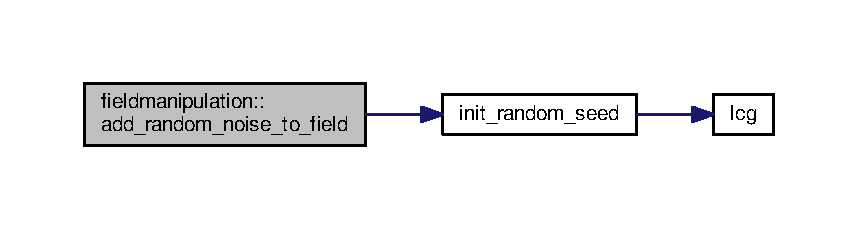
\includegraphics[width=350pt]{classfieldmanipulation_a3e8ca2ca22fb46938f8a479a82c90205_cgraph}
\end{center}
\end{figure}


\hypertarget{classfieldmanipulation_a8527c697c24116df3c60fce525a2c364}{\index{fieldmanipulation@{fieldmanipulation}!average@{average}}
\index{average@{average}!fieldmanipulation@{fieldmanipulation}}
\subsubsection[{average}]{\setlength{\rightskip}{0pt plus 5cm}real(dp) function, dimension(numcells) fieldmanipulation\-::average (
\begin{DoxyParamCaption}
\item[{real(dp), dimension(numtotal)}]{u}
\end{DoxyParamCaption}
)}}\label{classfieldmanipulation_a8527c697c24116df3c60fce525a2c364}


Here is the call graph for this function\-:\nopagebreak
\begin{figure}[H]
\begin{center}
\leavevmode
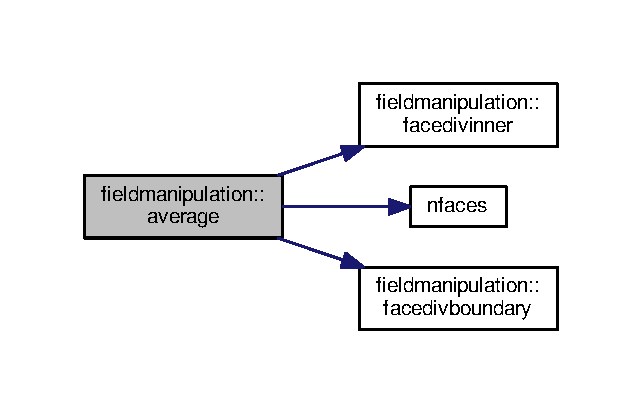
\includegraphics[width=308pt]{classfieldmanipulation_a8527c697c24116df3c60fce525a2c364_cgraph}
\end{center}
\end{figure}


\hypertarget{classfieldmanipulation_ad3594b987621ee1b66dc23373cba6482}{\index{fieldmanipulation@{fieldmanipulation}!calcpressdiv@{calcpressdiv}}
\index{calcpressdiv@{calcpressdiv}!fieldmanipulation@{fieldmanipulation}}
\subsubsection[{calcpressdiv}]{\setlength{\rightskip}{0pt plus 5cm}subroutine fieldmanipulation\-::calcpressdiv (
\begin{DoxyParamCaption}
{}
\end{DoxyParamCaption}
)}}\label{classfieldmanipulation_ad3594b987621ee1b66dc23373cba6482}


Here is the call graph for this function\-:\nopagebreak
\begin{figure}[H]
\begin{center}
\leavevmode
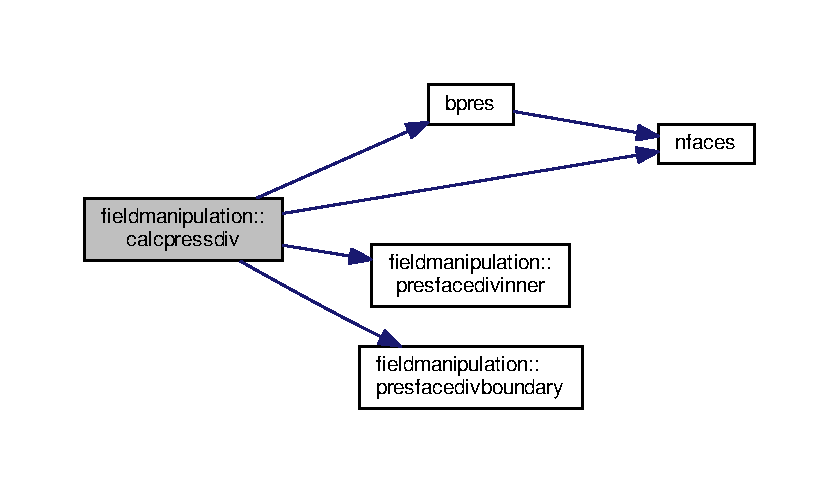
\includegraphics[width=350pt]{classfieldmanipulation_ad3594b987621ee1b66dc23373cba6482_cgraph}
\end{center}
\end{figure}


\hypertarget{classfieldmanipulation_aa58beed06659b15ede41acc5c6249991}{\index{fieldmanipulation@{fieldmanipulation}!expldiv@{expldiv}}
\index{expldiv@{expldiv}!fieldmanipulation@{fieldmanipulation}}
\subsubsection[{expldiv}]{\setlength{\rightskip}{0pt plus 5cm}real(dp) function, dimension(numcells) fieldmanipulation\-::expldiv (
\begin{DoxyParamCaption}
\item[{real(dp), dimension(numtotal)}]{u}
\end{DoxyParamCaption}
)}}\label{classfieldmanipulation_aa58beed06659b15ede41acc5c6249991}


Here is the call graph for this function\-:\nopagebreak
\begin{figure}[H]
\begin{center}
\leavevmode
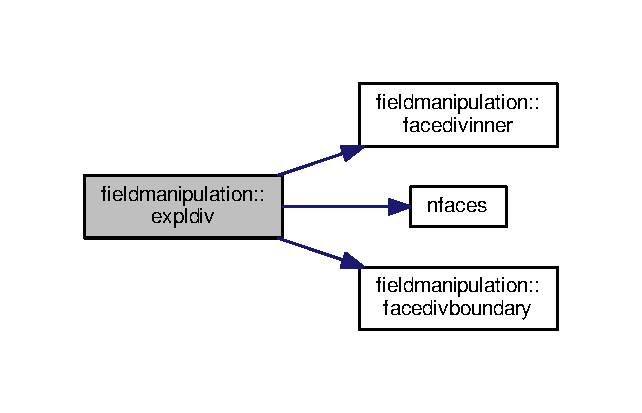
\includegraphics[width=308pt]{classfieldmanipulation_aa58beed06659b15ede41acc5c6249991_cgraph}
\end{center}
\end{figure}


\hypertarget{classfieldmanipulation_aa28be3da5dcf8b277c6c28391f01a06e}{\index{fieldmanipulation@{fieldmanipulation}!facedivboundary@{facedivboundary}}
\index{facedivboundary@{facedivboundary}!fieldmanipulation@{fieldmanipulation}}
\subsubsection[{facedivboundary}]{\setlength{\rightskip}{0pt plus 5cm}subroutine fieldmanipulation\-::facedivboundary (
\begin{DoxyParamCaption}
\item[{real(dp), intent(in)}]{sx, }
\item[{real(dp), intent(in)}]{sy, }
\item[{real(dp), intent(in)}]{sz, }
\item[{real(dp), intent(in)}]{fi, }
\item[{real(dp), intent(inout)}]{dfx}
\end{DoxyParamCaption}
)}}\label{classfieldmanipulation_aa28be3da5dcf8b277c6c28391f01a06e}
\hypertarget{classfieldmanipulation_afbd4007fedcd5c8960dfc4a3905349a9}{\index{fieldmanipulation@{fieldmanipulation}!facedivinner@{facedivinner}}
\index{facedivinner@{facedivinner}!fieldmanipulation@{fieldmanipulation}}
\subsubsection[{facedivinner}]{\setlength{\rightskip}{0pt plus 5cm}subroutine fieldmanipulation\-::facedivinner (
\begin{DoxyParamCaption}
\item[{integer, intent(in)}]{ijp, }
\item[{integer, intent(in)}]{ijn, }
\item[{real(dp), intent(in)}]{xfc, }
\item[{real(dp), intent(in)}]{yfc, }
\item[{real(dp), intent(in)}]{zfc, }
\item[{real(dp), intent(in)}]{sx, }
\item[{real(dp), intent(in)}]{sy, }
\item[{real(dp), intent(in)}]{sz, }
\item[{real(dp), intent(in)}]{fif, }
\item[{real(dp), dimension(numtotal), intent(in)}]{fi, }
\item[{real(dp), dimension(3,numcells), intent(in)}]{df, }
\item[{real(dp)}]{dfxe}
\end{DoxyParamCaption}
)}}\label{classfieldmanipulation_afbd4007fedcd5c8960dfc4a3905349a9}
\hypertarget{classfieldmanipulation_aba8cce868dfdd1d679c48022ed786ea8}{\index{fieldmanipulation@{fieldmanipulation}!faceinterpolatecdscorr@{faceinterpolatecdscorr}}
\index{faceinterpolatecdscorr@{faceinterpolatecdscorr}!fieldmanipulation@{fieldmanipulation}}
\subsubsection[{faceinterpolatecdscorr}]{\setlength{\rightskip}{0pt plus 5cm}subroutine fieldmanipulation\-::faceinterpolatecdscorr (
\begin{DoxyParamCaption}
\item[{integer, intent(in)}]{ijp, }
\item[{integer, intent(in)}]{ijn, }
\item[{real(dp), intent(in)}]{xfc, }
\item[{real(dp), intent(in)}]{yfc, }
\item[{real(dp), intent(in)}]{zfc, }
\item[{real(dp), intent(in)}]{fif, }
\item[{real(dp), dimension(numtotal), intent(in)}]{fi, }
\item[{real(dp), dimension(3,numcells), intent(in)}]{df, }
\item[{real(dp)}]{fie}
\end{DoxyParamCaption}
)}}\label{classfieldmanipulation_aba8cce868dfdd1d679c48022ed786ea8}
\hypertarget{classfieldmanipulation_abe2f38fcc53d73b51061465e3cf9e3dd}{\index{fieldmanipulation@{fieldmanipulation}!interpolate@{interpolate}}
\index{interpolate@{interpolate}!fieldmanipulation@{fieldmanipulation}}
\subsubsection[{interpolate}]{\setlength{\rightskip}{0pt plus 5cm}real(dp) function, dimension(numfaces) fieldmanipulation\-::interpolate (
\begin{DoxyParamCaption}
\item[{real(dp), dimension(numtotal)}]{u}
\end{DoxyParamCaption}
)}}\label{classfieldmanipulation_abe2f38fcc53d73b51061465e3cf9e3dd}


Here is the call graph for this function\-:\nopagebreak
\begin{figure}[H]
\begin{center}
\leavevmode
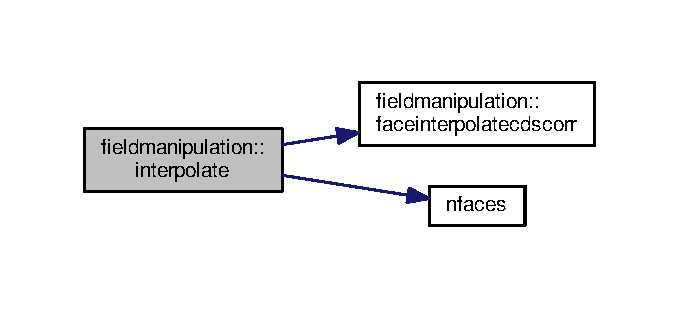
\includegraphics[width=326pt]{classfieldmanipulation_abe2f38fcc53d73b51061465e3cf9e3dd_cgraph}
\end{center}
\end{figure}


\hypertarget{classfieldmanipulation_afe436887e04bd6717076c2bee1210f19}{\index{fieldmanipulation@{fieldmanipulation}!presfacedivboundary@{presfacedivboundary}}
\index{presfacedivboundary@{presfacedivboundary}!fieldmanipulation@{fieldmanipulation}}
\subsubsection[{presfacedivboundary}]{\setlength{\rightskip}{0pt plus 5cm}subroutine fieldmanipulation\-::presfacedivboundary (
\begin{DoxyParamCaption}
\item[{real(dp), intent(in)}]{sx, }
\item[{real(dp), intent(in)}]{sy, }
\item[{real(dp), intent(in)}]{sz, }
\item[{real(dp), intent(in)}]{fi, }
\item[{real(dp), intent(inout)}]{dfx, }
\item[{real(dp), intent(inout)}]{dfy, }
\item[{real(dp), intent(inout)}]{dfz}
\end{DoxyParamCaption}
)}}\label{classfieldmanipulation_afe436887e04bd6717076c2bee1210f19}
\hypertarget{classfieldmanipulation_a8fa4949333251cce2f68dd0566a71e7b}{\index{fieldmanipulation@{fieldmanipulation}!presfacedivinner@{presfacedivinner}}
\index{presfacedivinner@{presfacedivinner}!fieldmanipulation@{fieldmanipulation}}
\subsubsection[{presfacedivinner}]{\setlength{\rightskip}{0pt plus 5cm}subroutine fieldmanipulation\-::presfacedivinner (
\begin{DoxyParamCaption}
\item[{integer, intent(in)}]{ijp, }
\item[{integer, intent(in)}]{ijn, }
\item[{real(dp), intent(in)}]{xfc, }
\item[{real(dp), intent(in)}]{yfc, }
\item[{real(dp), intent(in)}]{zfc, }
\item[{real(dp), intent(in)}]{sx, }
\item[{real(dp), intent(in)}]{sy, }
\item[{real(dp), intent(in)}]{sz, }
\item[{real(dp), intent(in)}]{fif, }
\item[{real(dp), dimension(numtotal), intent(in)}]{fi, }
\item[{real(dp), dimension(3,numcells), intent(in)}]{df, }
\item[{real(dp)}]{dfxe, }
\item[{real(dp)}]{dfye, }
\item[{real(dp)}]{dfze}
\end{DoxyParamCaption}
)}}\label{classfieldmanipulation_a8fa4949333251cce2f68dd0566a71e7b}
\hypertarget{classfieldmanipulation_a3212f37b15b79464ad49e662e2a5a394}{\index{fieldmanipulation@{fieldmanipulation}!surfaceintegrate@{surfaceintegrate}}
\index{surfaceintegrate@{surfaceintegrate}!fieldmanipulation@{fieldmanipulation}}
\subsubsection[{surfaceintegrate}]{\setlength{\rightskip}{0pt plus 5cm}real(dp) function, dimension(numcells) fieldmanipulation\-::surfaceintegrate (
\begin{DoxyParamCaption}
\item[{real(dp), dimension(numtotal)}]{u}
\end{DoxyParamCaption}
)}}\label{classfieldmanipulation_a3212f37b15b79464ad49e662e2a5a394}


Here is the call graph for this function\-:\nopagebreak
\begin{figure}[H]
\begin{center}
\leavevmode
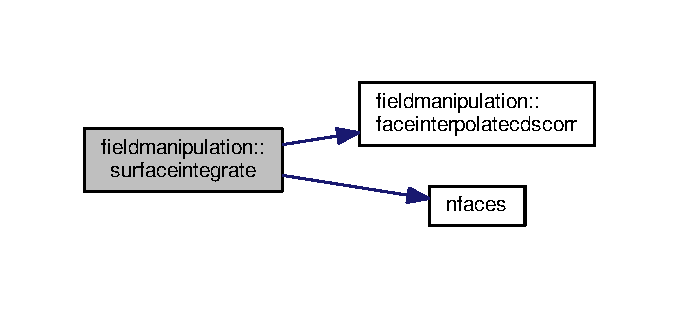
\includegraphics[width=326pt]{classfieldmanipulation_a3212f37b15b79464ad49e662e2a5a394_cgraph}
\end{center}
\end{figure}


\hypertarget{classfieldmanipulation_a3f3fb8bda2659dd1f034ef8c5a99b405}{\index{fieldmanipulation@{fieldmanipulation}!surfacesum@{surfacesum}}
\index{surfacesum@{surfacesum}!fieldmanipulation@{fieldmanipulation}}
\subsubsection[{surfacesum}]{\setlength{\rightskip}{0pt plus 5cm}real(dp) function, dimension(numcells) fieldmanipulation\-::surfacesum (
\begin{DoxyParamCaption}
\item[{real(dp), dimension(numtotal)}]{u}
\end{DoxyParamCaption}
)}}\label{classfieldmanipulation_a3f3fb8bda2659dd1f034ef8c5a99b405}


Here is the call graph for this function\-:\nopagebreak
\begin{figure}[H]
\begin{center}
\leavevmode
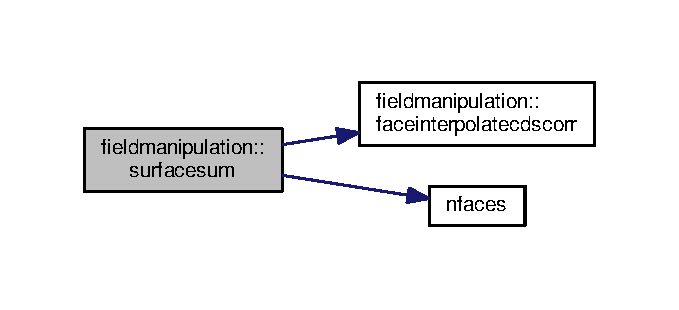
\includegraphics[width=326pt]{classfieldmanipulation_a3f3fb8bda2659dd1f034ef8c5a99b405_cgraph}
\end{center}
\end{figure}


\hypertarget{classfieldmanipulation_a0bdf9e1dcd8cee01d2a1f90bb96a1583}{\index{fieldmanipulation@{fieldmanipulation}!volumeweightedaverage@{volumeweightedaverage}}
\index{volumeweightedaverage@{volumeweightedaverage}!fieldmanipulation@{fieldmanipulation}}
\subsubsection[{volumeweightedaverage}]{\setlength{\rightskip}{0pt plus 5cm}real(dp) function fieldmanipulation\-::volumeweightedaverage (
\begin{DoxyParamCaption}
\item[{real(dp), dimension(numtotal), intent(in)}]{U}
\end{DoxyParamCaption}
)}}\label{classfieldmanipulation_a0bdf9e1dcd8cee01d2a1f90bb96a1583}


Here is the call graph for this function\-:\nopagebreak
\begin{figure}[H]
\begin{center}
\leavevmode
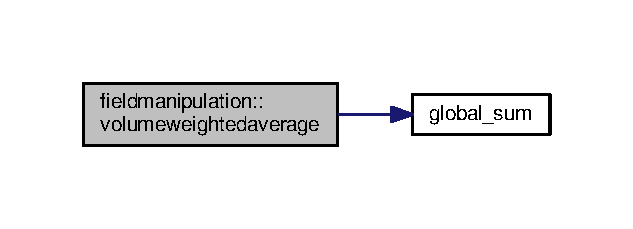
\includegraphics[width=304pt]{classfieldmanipulation_a0bdf9e1dcd8cee01d2a1f90bb96a1583_cgraph}
\end{center}
\end{figure}




The documentation for this module was generated from the following file\-:\begin{DoxyCompactItemize}
\item 
src-\/par/\hyperlink{fieldManipulation_8f90}{field\-Manipulation.\-f90}\end{DoxyCompactItemize}

\hypertarget{classfv__equation}{\section{fv\-\_\-equation Module Reference}
\label{classfv__equation}\index{fv\-\_\-equation@{fv\-\_\-equation}}
}
\subsection*{Data Types}
\begin{DoxyCompactItemize}
\item 
type \hyperlink{structfv__equation_1_1fvequation}{fvequation}
\item 
type \hyperlink{structfv__equation_1_1fvvectorequation}{fvvectorequation}
\item 
interface \hyperlink{interfacefv__equation_1_1operator_07_09_08}{operator(+)}
\item 
interface \hyperlink{interfacefv__equation_1_1operator_07-_08}{operator(-\/)}
\item 
interface \hyperlink{interfacefv__equation_1_1operator_07_0A_0A_08}{operator(==)}
\end{DoxyCompactItemize}
\subsection*{Public Member Functions}
\begin{DoxyCompactItemize}
\item 
type(csrmatrix) function \hyperlink{classfv__equation_a6cdef646079ec69baf08f18aba78f6a9}{new\-\_\-csrmatrix} ()
\item 
type(\hyperlink{structfv__equation_1_1fvequation}{fvequation}) function \hyperlink{classfv__equation_a26481f97d53ea82c43a66a0b31e73a4e}{new\-\_\-fvequation} ()
\item 
type(\hyperlink{structfv__equation_1_1fvvectorequation}{fvvectorequation}) function \hyperlink{classfv__equation_ab46a4f94deb0186ea0798d62c34f2cae}{new\-\_\-fvvectorequation} ()
\item 
type(\hyperlink{structfv__equation_1_1fvequation}{fvequation}) function \hyperlink{classfv__equation_a642df53156dacdf9e8cfb78a4a80afbc}{add\-\_\-source\-\_\-to\-\_\-fvequation} (fv\-Eqn\-In, source)
\item 
type(\hyperlink{structfv__equation_1_1fvvectorequation}{fvvectorequation}) function \hyperlink{classfv__equation_a1cd42802fcacf44f5388489bd3df7c67}{add\-\_\-volvectorfieldsource\-\_\-to\-\_\-fvvectorequation} (fv\-Eqn\-In, vec\-Source)
\item 
type(\hyperlink{structfv__equation_1_1fvequation}{fvequation}) function \hyperlink{classfv__equation_ad6aa7075e57df58366c29f5015c0865e}{substract\-\_\-source\-\_\-from\-\_\-fvequation} (fv\-Eqn\-In, source)
\item 
type(\hyperlink{structfv__equation_1_1fvvectorequation}{fvvectorequation}) function \hyperlink{classfv__equation_a3d4afbd5ad280d482ba99f117913ecd4}{substract\-\_\-volvectorfieldsource\-\_\-from\-\_\-fvvectorequation} (fv\-Eqn, vec\-Source)
\item 
type(\hyperlink{structfv__equation_1_1fvequation}{fvequation}) function \hyperlink{classfv__equation_a0097d3c782d694764ed35de4b8846746}{add\-\_\-fvequations} (fv\-Eqn1, fv\-Eqn2)
\item 
type(\hyperlink{structfv__equation_1_1fvvectorequation}{fvvectorequation}) function \hyperlink{classfv__equation_adde0fa2f08474e2a33743d27a38cd813}{add\-\_\-fvvectorequations} (fv\-Eqn1, fv\-Eqn2)
\item 
type(\hyperlink{structfv__equation_1_1fvequation}{fvequation}) function \hyperlink{classfv__equation_ab635143c726e64626d65e59962cd4f5e}{substract\-\_\-fvequations} (fv\-Eqn1, fv\-Eqn2)
\item 
type(\hyperlink{structfv__equation_1_1fvvectorequation}{fvvectorequation}) function \hyperlink{classfv__equation_a7da2e0fbfe99bc1e49cc62c9a970ba48}{substract\-\_\-fvvectorequations} (fv\-Eqn1, fv\-Eqn2)
\end{DoxyCompactItemize}


\subsection{Member Function/\-Subroutine Documentation}
\hypertarget{classfv__equation_a0097d3c782d694764ed35de4b8846746}{\index{fv\-\_\-equation@{fv\-\_\-equation}!add\-\_\-fvequations@{add\-\_\-fvequations}}
\index{add\-\_\-fvequations@{add\-\_\-fvequations}!fv_equation@{fv\-\_\-equation}}
\subsubsection[{add\-\_\-fvequations}]{\setlength{\rightskip}{0pt plus 5cm}type({\bf fvequation}) function fv\-\_\-equation\-::add\-\_\-fvequations (
\begin{DoxyParamCaption}
\item[{type({\bf fvequation}), intent(in)}]{fv\-Eqn1, }
\item[{type({\bf fvequation}), intent(in)}]{fv\-Eqn2}
\end{DoxyParamCaption}
)}}\label{classfv__equation_a0097d3c782d694764ed35de4b8846746}


Here is the call graph for this function\-:\nopagebreak
\begin{figure}[H]
\begin{center}
\leavevmode
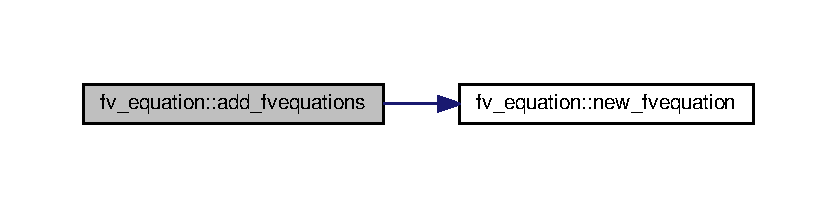
\includegraphics[width=350pt]{classfv__equation_a0097d3c782d694764ed35de4b8846746_cgraph}
\end{center}
\end{figure}


\hypertarget{classfv__equation_adde0fa2f08474e2a33743d27a38cd813}{\index{fv\-\_\-equation@{fv\-\_\-equation}!add\-\_\-fvvectorequations@{add\-\_\-fvvectorequations}}
\index{add\-\_\-fvvectorequations@{add\-\_\-fvvectorequations}!fv_equation@{fv\-\_\-equation}}
\subsubsection[{add\-\_\-fvvectorequations}]{\setlength{\rightskip}{0pt plus 5cm}type({\bf fvvectorequation}) function fv\-\_\-equation\-::add\-\_\-fvvectorequations (
\begin{DoxyParamCaption}
\item[{type({\bf fvvectorequation}), intent(in)}]{fv\-Eqn1, }
\item[{type({\bf fvvectorequation}), intent(in)}]{fv\-Eqn2}
\end{DoxyParamCaption}
)}}\label{classfv__equation_adde0fa2f08474e2a33743d27a38cd813}


Here is the call graph for this function\-:\nopagebreak
\begin{figure}[H]
\begin{center}
\leavevmode
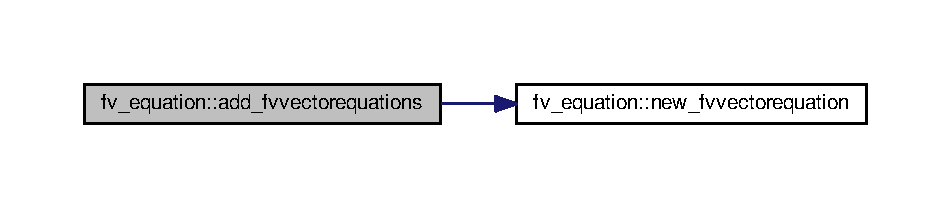
\includegraphics[width=350pt]{classfv__equation_adde0fa2f08474e2a33743d27a38cd813_cgraph}
\end{center}
\end{figure}


\hypertarget{classfv__equation_a642df53156dacdf9e8cfb78a4a80afbc}{\index{fv\-\_\-equation@{fv\-\_\-equation}!add\-\_\-source\-\_\-to\-\_\-fvequation@{add\-\_\-source\-\_\-to\-\_\-fvequation}}
\index{add\-\_\-source\-\_\-to\-\_\-fvequation@{add\-\_\-source\-\_\-to\-\_\-fvequation}!fv_equation@{fv\-\_\-equation}}
\subsubsection[{add\-\_\-source\-\_\-to\-\_\-fvequation}]{\setlength{\rightskip}{0pt plus 5cm}type({\bf fvequation}) function fv\-\_\-equation\-::add\-\_\-source\-\_\-to\-\_\-fvequation (
\begin{DoxyParamCaption}
\item[{type({\bf fvequation}), intent(in)}]{fv\-Eqn\-In, }
\item[{type(volscalarfield), intent(in)}]{source}
\end{DoxyParamCaption}
)}}\label{classfv__equation_a642df53156dacdf9e8cfb78a4a80afbc}


Here is the call graph for this function\-:\nopagebreak
\begin{figure}[H]
\begin{center}
\leavevmode
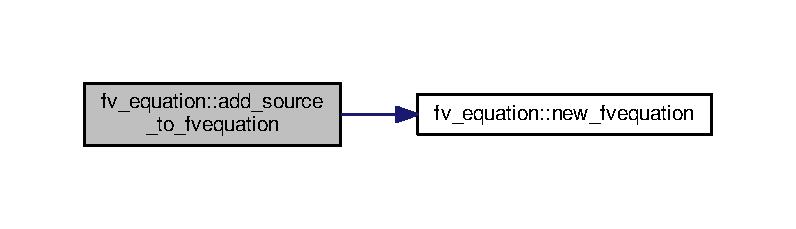
\includegraphics[width=350pt]{classfv__equation_a642df53156dacdf9e8cfb78a4a80afbc_cgraph}
\end{center}
\end{figure}


\hypertarget{classfv__equation_a1cd42802fcacf44f5388489bd3df7c67}{\index{fv\-\_\-equation@{fv\-\_\-equation}!add\-\_\-volvectorfieldsource\-\_\-to\-\_\-fvvectorequation@{add\-\_\-volvectorfieldsource\-\_\-to\-\_\-fvvectorequation}}
\index{add\-\_\-volvectorfieldsource\-\_\-to\-\_\-fvvectorequation@{add\-\_\-volvectorfieldsource\-\_\-to\-\_\-fvvectorequation}!fv_equation@{fv\-\_\-equation}}
\subsubsection[{add\-\_\-volvectorfieldsource\-\_\-to\-\_\-fvvectorequation}]{\setlength{\rightskip}{0pt plus 5cm}type({\bf fvvectorequation}) function fv\-\_\-equation\-::add\-\_\-volvectorfieldsource\-\_\-to\-\_\-fvvectorequation (
\begin{DoxyParamCaption}
\item[{type({\bf fvvectorequation}), intent(in)}]{fv\-Eqn\-In, }
\item[{type(volvectorfield), intent(in)}]{vec\-Source}
\end{DoxyParamCaption}
)}}\label{classfv__equation_a1cd42802fcacf44f5388489bd3df7c67}


Here is the call graph for this function\-:\nopagebreak
\begin{figure}[H]
\begin{center}
\leavevmode
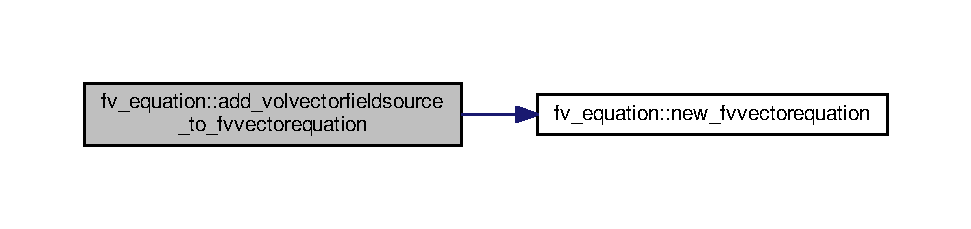
\includegraphics[width=350pt]{classfv__equation_a1cd42802fcacf44f5388489bd3df7c67_cgraph}
\end{center}
\end{figure}


\hypertarget{classfv__equation_a6cdef646079ec69baf08f18aba78f6a9}{\index{fv\-\_\-equation@{fv\-\_\-equation}!new\-\_\-csrmatrix@{new\-\_\-csrmatrix}}
\index{new\-\_\-csrmatrix@{new\-\_\-csrmatrix}!fv_equation@{fv\-\_\-equation}}
\subsubsection[{new\-\_\-csrmatrix}]{\setlength{\rightskip}{0pt plus 5cm}type(csrmatrix) function fv\-\_\-equation\-::new\-\_\-csrmatrix (
\begin{DoxyParamCaption}
{}
\end{DoxyParamCaption}
)}}\label{classfv__equation_a6cdef646079ec69baf08f18aba78f6a9}
\hypertarget{classfv__equation_a26481f97d53ea82c43a66a0b31e73a4e}{\index{fv\-\_\-equation@{fv\-\_\-equation}!new\-\_\-fvequation@{new\-\_\-fvequation}}
\index{new\-\_\-fvequation@{new\-\_\-fvequation}!fv_equation@{fv\-\_\-equation}}
\subsubsection[{new\-\_\-fvequation}]{\setlength{\rightskip}{0pt plus 5cm}type({\bf fvequation}) function fv\-\_\-equation\-::new\-\_\-fvequation (
\begin{DoxyParamCaption}
{}
\end{DoxyParamCaption}
)}}\label{classfv__equation_a26481f97d53ea82c43a66a0b31e73a4e}
\hypertarget{classfv__equation_ab46a4f94deb0186ea0798d62c34f2cae}{\index{fv\-\_\-equation@{fv\-\_\-equation}!new\-\_\-fvvectorequation@{new\-\_\-fvvectorequation}}
\index{new\-\_\-fvvectorequation@{new\-\_\-fvvectorequation}!fv_equation@{fv\-\_\-equation}}
\subsubsection[{new\-\_\-fvvectorequation}]{\setlength{\rightskip}{0pt plus 5cm}type({\bf fvvectorequation}) function fv\-\_\-equation\-::new\-\_\-fvvectorequation (
\begin{DoxyParamCaption}
{}
\end{DoxyParamCaption}
)}}\label{classfv__equation_ab46a4f94deb0186ea0798d62c34f2cae}
\hypertarget{classfv__equation_ab635143c726e64626d65e59962cd4f5e}{\index{fv\-\_\-equation@{fv\-\_\-equation}!substract\-\_\-fvequations@{substract\-\_\-fvequations}}
\index{substract\-\_\-fvequations@{substract\-\_\-fvequations}!fv_equation@{fv\-\_\-equation}}
\subsubsection[{substract\-\_\-fvequations}]{\setlength{\rightskip}{0pt plus 5cm}type({\bf fvequation}) function fv\-\_\-equation\-::substract\-\_\-fvequations (
\begin{DoxyParamCaption}
\item[{type({\bf fvequation}), intent(in)}]{fv\-Eqn1, }
\item[{type({\bf fvequation}), intent(in)}]{fv\-Eqn2}
\end{DoxyParamCaption}
)}}\label{classfv__equation_ab635143c726e64626d65e59962cd4f5e}


Here is the call graph for this function\-:\nopagebreak
\begin{figure}[H]
\begin{center}
\leavevmode
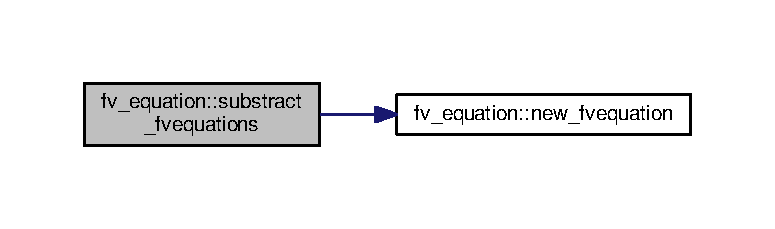
\includegraphics[width=350pt]{classfv__equation_ab635143c726e64626d65e59962cd4f5e_cgraph}
\end{center}
\end{figure}


\hypertarget{classfv__equation_a7da2e0fbfe99bc1e49cc62c9a970ba48}{\index{fv\-\_\-equation@{fv\-\_\-equation}!substract\-\_\-fvvectorequations@{substract\-\_\-fvvectorequations}}
\index{substract\-\_\-fvvectorequations@{substract\-\_\-fvvectorequations}!fv_equation@{fv\-\_\-equation}}
\subsubsection[{substract\-\_\-fvvectorequations}]{\setlength{\rightskip}{0pt plus 5cm}type({\bf fvvectorequation}) function fv\-\_\-equation\-::substract\-\_\-fvvectorequations (
\begin{DoxyParamCaption}
\item[{type({\bf fvvectorequation}), intent(in)}]{fv\-Eqn1, }
\item[{type({\bf fvvectorequation}), intent(in)}]{fv\-Eqn2}
\end{DoxyParamCaption}
)}}\label{classfv__equation_a7da2e0fbfe99bc1e49cc62c9a970ba48}


Here is the call graph for this function\-:\nopagebreak
\begin{figure}[H]
\begin{center}
\leavevmode
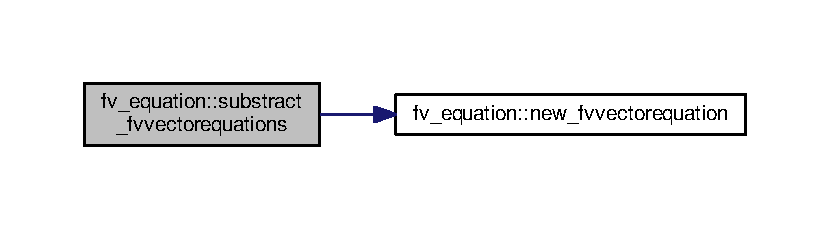
\includegraphics[width=350pt]{classfv__equation_a7da2e0fbfe99bc1e49cc62c9a970ba48_cgraph}
\end{center}
\end{figure}


\hypertarget{classfv__equation_ad6aa7075e57df58366c29f5015c0865e}{\index{fv\-\_\-equation@{fv\-\_\-equation}!substract\-\_\-source\-\_\-from\-\_\-fvequation@{substract\-\_\-source\-\_\-from\-\_\-fvequation}}
\index{substract\-\_\-source\-\_\-from\-\_\-fvequation@{substract\-\_\-source\-\_\-from\-\_\-fvequation}!fv_equation@{fv\-\_\-equation}}
\subsubsection[{substract\-\_\-source\-\_\-from\-\_\-fvequation}]{\setlength{\rightskip}{0pt plus 5cm}type({\bf fvequation}) function fv\-\_\-equation\-::substract\-\_\-source\-\_\-from\-\_\-fvequation (
\begin{DoxyParamCaption}
\item[{type({\bf fvequation}), intent(in)}]{fv\-Eqn\-In, }
\item[{type(volscalarfield), intent(in)}]{source}
\end{DoxyParamCaption}
)}}\label{classfv__equation_ad6aa7075e57df58366c29f5015c0865e}


Here is the call graph for this function\-:\nopagebreak
\begin{figure}[H]
\begin{center}
\leavevmode
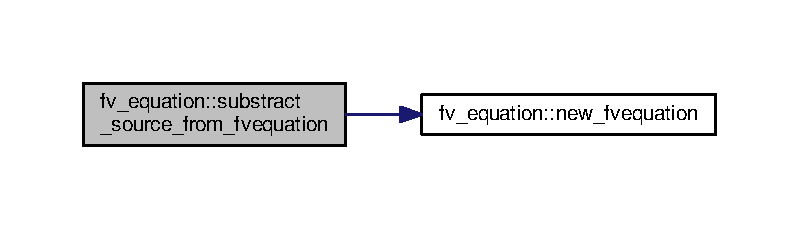
\includegraphics[width=350pt]{classfv__equation_ad6aa7075e57df58366c29f5015c0865e_cgraph}
\end{center}
\end{figure}


\hypertarget{classfv__equation_a3d4afbd5ad280d482ba99f117913ecd4}{\index{fv\-\_\-equation@{fv\-\_\-equation}!substract\-\_\-volvectorfieldsource\-\_\-from\-\_\-fvvectorequation@{substract\-\_\-volvectorfieldsource\-\_\-from\-\_\-fvvectorequation}}
\index{substract\-\_\-volvectorfieldsource\-\_\-from\-\_\-fvvectorequation@{substract\-\_\-volvectorfieldsource\-\_\-from\-\_\-fvvectorequation}!fv_equation@{fv\-\_\-equation}}
\subsubsection[{substract\-\_\-volvectorfieldsource\-\_\-from\-\_\-fvvectorequation}]{\setlength{\rightskip}{0pt plus 5cm}type({\bf fvvectorequation}) function fv\-\_\-equation\-::substract\-\_\-volvectorfieldsource\-\_\-from\-\_\-fvvectorequation (
\begin{DoxyParamCaption}
\item[{type({\bf fvvectorequation}), intent(in)}]{fv\-Eqn, }
\item[{type(volvectorfield), intent(in)}]{vec\-Source}
\end{DoxyParamCaption}
)}}\label{classfv__equation_a3d4afbd5ad280d482ba99f117913ecd4}


Here is the call graph for this function\-:\nopagebreak
\begin{figure}[H]
\begin{center}
\leavevmode
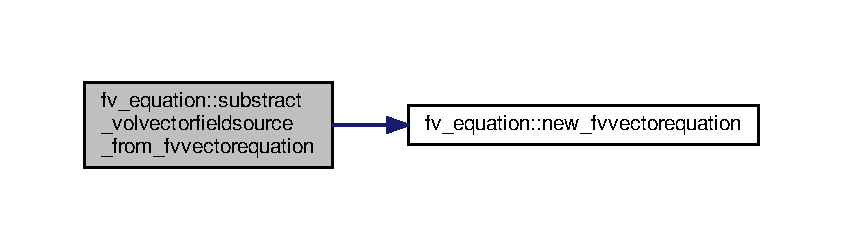
\includegraphics[width=350pt]{classfv__equation_a3d4afbd5ad280d482ba99f117913ecd4_cgraph}
\end{center}
\end{figure}




The documentation for this module was generated from the following file\-:\begin{DoxyCompactItemize}
\item 
src-\/par/\hyperlink{fv__equation_8f90}{fv\-\_\-equation.\-f90}\end{DoxyCompactItemize}

\hypertarget{structfv__equation_1_1fvequation}{}\doxysection{fv\+\_\+equation\+::fvequation Type Reference}
\label{structfv__equation_1_1fvequation}\index{fv\_equation::fvequation@{fv\_equation::fvequation}}


Inheritance diagram for fv\+\_\+equation\+::fvequation\+:
% FIG 0


Collaboration diagram for fv\+\_\+equation\+::fvequation\+:
% FIG 1
\doxysubsection*{Public Attributes}
\begin{DoxyCompactItemize}
\item 
real(dp), dimension(\+:), allocatable \mbox{\hyperlink{structfv__equation_1_1fvequation_a5e62f6aa9945885b4569e307c550f1f7}{source}}
\item 
real(dp), dimension(\+:), allocatable \mbox{\hyperlink{structfv__equation_1_1fvequation_ad6a75f5fc5341eeee3247dc71286bd24}{o}}
\item 
real(dp), dimension(\+:), allocatable \mbox{\hyperlink{structfv__equation_1_1fvequation_ab71f5aa786a1f668f5389e466db9ade8}{oo}}
\end{DoxyCompactItemize}


\doxysubsection{Member Data Documentation}
\mbox{\Hypertarget{structfv__equation_1_1fvequation_ad6a75f5fc5341eeee3247dc71286bd24}\label{structfv__equation_1_1fvequation_ad6a75f5fc5341eeee3247dc71286bd24}} 
\index{fv\_equation::fvequation@{fv\_equation::fvequation}!o@{o}}
\index{o@{o}!fv\_equation::fvequation@{fv\_equation::fvequation}}
\doxysubsubsection{\texorpdfstring{o}{o}}
{\footnotesize\ttfamily real(dp), dimension(\+:), allocatable fv\+\_\+equation\+::fvequation\+::o}

\mbox{\Hypertarget{structfv__equation_1_1fvequation_ab71f5aa786a1f668f5389e466db9ade8}\label{structfv__equation_1_1fvequation_ab71f5aa786a1f668f5389e466db9ade8}} 
\index{fv\_equation::fvequation@{fv\_equation::fvequation}!oo@{oo}}
\index{oo@{oo}!fv\_equation::fvequation@{fv\_equation::fvequation}}
\doxysubsubsection{\texorpdfstring{oo}{oo}}
{\footnotesize\ttfamily real(dp), dimension(\+:), allocatable fv\+\_\+equation\+::fvequation\+::oo}

\mbox{\Hypertarget{structfv__equation_1_1fvequation_a5e62f6aa9945885b4569e307c550f1f7}\label{structfv__equation_1_1fvequation_a5e62f6aa9945885b4569e307c550f1f7}} 
\index{fv\_equation::fvequation@{fv\_equation::fvequation}!source@{source}}
\index{source@{source}!fv\_equation::fvequation@{fv\_equation::fvequation}}
\doxysubsubsection{\texorpdfstring{source}{source}}
{\footnotesize\ttfamily real(dp), dimension(\+:), allocatable fv\+\_\+equation\+::fvequation\+::source}



The documentation for this type was generated from the following file\+:\begin{DoxyCompactItemize}
\item 
src-\/par/\mbox{\hyperlink{fv__equation_8f90}{fv\+\_\+equation.\+f90}}\end{DoxyCompactItemize}

\hypertarget{structfv__equation_1_1fvvectorequation}{}\doxysection{fv\+\_\+equation\+::fvvectorequation Type Reference}
\label{structfv__equation_1_1fvvectorequation}\index{fv\_equation::fvvectorequation@{fv\_equation::fvvectorequation}}


Inheritance diagram for fv\+\_\+equation\+::fvvectorequation\+:
% FIG 0


Collaboration diagram for fv\+\_\+equation\+::fvvectorequation\+:
% FIG 1
\doxysubsection*{Public Attributes}
\begin{DoxyCompactItemize}
\item 
real(dp), dimension(\+:), allocatable \mbox{\hyperlink{structfv__equation_1_1fvvectorequation_a7f44e6ac5ffa1baa495dd13137ef8be7}{spu}}
\item 
real(dp), dimension(\+:), allocatable \mbox{\hyperlink{structfv__equation_1_1fvvectorequation_a33b72db8fdfb8122c72fe2e5a9593eb1}{spv}}
\item 
real(dp), dimension(\+:), allocatable \mbox{\hyperlink{structfv__equation_1_1fvvectorequation_aa15bb4a30555344af9fdb0817b411544}{spw}}
\item 
real(dp), dimension(\+:), allocatable \mbox{\hyperlink{structfv__equation_1_1fvvectorequation_ad955a3b8ed3260f8f97d94515f95a9b5}{su}}
\item 
real(dp), dimension(\+:), allocatable \mbox{\hyperlink{structfv__equation_1_1fvvectorequation_ab1cbe6f0b271700792f9b854acbf5174}{sv}}
\item 
real(dp), dimension(\+:), allocatable \mbox{\hyperlink{structfv__equation_1_1fvvectorequation_a35835e2b67a385850608de4a6cd0456c}{sw}}
\item 
real(dp), dimension(\+:), allocatable \mbox{\hyperlink{structfv__equation_1_1fvvectorequation_aa8f4bd07b31af4434d8e33dc06b402e5}{xo}}
\item 
real(dp), dimension(\+:), allocatable \mbox{\hyperlink{structfv__equation_1_1fvvectorequation_ac2446def37d90a8809b2c3998de30c8e}{yo}}
\item 
real(dp), dimension(\+:), allocatable \mbox{\hyperlink{structfv__equation_1_1fvvectorequation_a6722be7e3093855814a40ce85ec58508}{zo}}
\item 
real(dp), dimension(\+:), allocatable \mbox{\hyperlink{structfv__equation_1_1fvvectorequation_ac4a216c8f3ffa2d167b6b0cab25801ef}{xoo}}
\item 
real(dp), dimension(\+:), allocatable \mbox{\hyperlink{structfv__equation_1_1fvvectorequation_a1631b0c62d09b603309dfa754a31a7fd}{yoo}}
\item 
real(dp), dimension(\+:), allocatable \mbox{\hyperlink{structfv__equation_1_1fvvectorequation_a890fa380a32227ef9e1b33590357076c}{zoo}}
\end{DoxyCompactItemize}


\doxysubsection{Member Data Documentation}
\mbox{\Hypertarget{structfv__equation_1_1fvvectorequation_a7f44e6ac5ffa1baa495dd13137ef8be7}\label{structfv__equation_1_1fvvectorequation_a7f44e6ac5ffa1baa495dd13137ef8be7}} 
\index{fv\_equation::fvvectorequation@{fv\_equation::fvvectorequation}!spu@{spu}}
\index{spu@{spu}!fv\_equation::fvvectorequation@{fv\_equation::fvvectorequation}}
\doxysubsubsection{\texorpdfstring{spu}{spu}}
{\footnotesize\ttfamily real(dp), dimension(\+:), allocatable fv\+\_\+equation\+::fvvectorequation\+::spu}

\mbox{\Hypertarget{structfv__equation_1_1fvvectorequation_a33b72db8fdfb8122c72fe2e5a9593eb1}\label{structfv__equation_1_1fvvectorequation_a33b72db8fdfb8122c72fe2e5a9593eb1}} 
\index{fv\_equation::fvvectorequation@{fv\_equation::fvvectorequation}!spv@{spv}}
\index{spv@{spv}!fv\_equation::fvvectorequation@{fv\_equation::fvvectorequation}}
\doxysubsubsection{\texorpdfstring{spv}{spv}}
{\footnotesize\ttfamily real(dp), dimension(\+:), allocatable fv\+\_\+equation\+::fvvectorequation\+::spv}

\mbox{\Hypertarget{structfv__equation_1_1fvvectorequation_aa15bb4a30555344af9fdb0817b411544}\label{structfv__equation_1_1fvvectorequation_aa15bb4a30555344af9fdb0817b411544}} 
\index{fv\_equation::fvvectorequation@{fv\_equation::fvvectorequation}!spw@{spw}}
\index{spw@{spw}!fv\_equation::fvvectorequation@{fv\_equation::fvvectorequation}}
\doxysubsubsection{\texorpdfstring{spw}{spw}}
{\footnotesize\ttfamily real(dp), dimension(\+:), allocatable fv\+\_\+equation\+::fvvectorequation\+::spw}

\mbox{\Hypertarget{structfv__equation_1_1fvvectorequation_ad955a3b8ed3260f8f97d94515f95a9b5}\label{structfv__equation_1_1fvvectorequation_ad955a3b8ed3260f8f97d94515f95a9b5}} 
\index{fv\_equation::fvvectorequation@{fv\_equation::fvvectorequation}!su@{su}}
\index{su@{su}!fv\_equation::fvvectorequation@{fv\_equation::fvvectorequation}}
\doxysubsubsection{\texorpdfstring{su}{su}}
{\footnotesize\ttfamily real(dp), dimension(\+:), allocatable fv\+\_\+equation\+::fvvectorequation\+::su}

\mbox{\Hypertarget{structfv__equation_1_1fvvectorequation_ab1cbe6f0b271700792f9b854acbf5174}\label{structfv__equation_1_1fvvectorequation_ab1cbe6f0b271700792f9b854acbf5174}} 
\index{fv\_equation::fvvectorequation@{fv\_equation::fvvectorequation}!sv@{sv}}
\index{sv@{sv}!fv\_equation::fvvectorequation@{fv\_equation::fvvectorequation}}
\doxysubsubsection{\texorpdfstring{sv}{sv}}
{\footnotesize\ttfamily real(dp), dimension(\+:), allocatable fv\+\_\+equation\+::fvvectorequation\+::sv}

\mbox{\Hypertarget{structfv__equation_1_1fvvectorequation_a35835e2b67a385850608de4a6cd0456c}\label{structfv__equation_1_1fvvectorequation_a35835e2b67a385850608de4a6cd0456c}} 
\index{fv\_equation::fvvectorequation@{fv\_equation::fvvectorequation}!sw@{sw}}
\index{sw@{sw}!fv\_equation::fvvectorequation@{fv\_equation::fvvectorequation}}
\doxysubsubsection{\texorpdfstring{sw}{sw}}
{\footnotesize\ttfamily real(dp), dimension(\+:), allocatable fv\+\_\+equation\+::fvvectorequation\+::sw}

\mbox{\Hypertarget{structfv__equation_1_1fvvectorequation_aa8f4bd07b31af4434d8e33dc06b402e5}\label{structfv__equation_1_1fvvectorequation_aa8f4bd07b31af4434d8e33dc06b402e5}} 
\index{fv\_equation::fvvectorequation@{fv\_equation::fvvectorequation}!xo@{xo}}
\index{xo@{xo}!fv\_equation::fvvectorequation@{fv\_equation::fvvectorequation}}
\doxysubsubsection{\texorpdfstring{xo}{xo}}
{\footnotesize\ttfamily real(dp), dimension(\+:), allocatable fv\+\_\+equation\+::fvvectorequation\+::xo}

\mbox{\Hypertarget{structfv__equation_1_1fvvectorequation_ac4a216c8f3ffa2d167b6b0cab25801ef}\label{structfv__equation_1_1fvvectorequation_ac4a216c8f3ffa2d167b6b0cab25801ef}} 
\index{fv\_equation::fvvectorequation@{fv\_equation::fvvectorequation}!xoo@{xoo}}
\index{xoo@{xoo}!fv\_equation::fvvectorequation@{fv\_equation::fvvectorequation}}
\doxysubsubsection{\texorpdfstring{xoo}{xoo}}
{\footnotesize\ttfamily real(dp), dimension(\+:), allocatable fv\+\_\+equation\+::fvvectorequation\+::xoo}

\mbox{\Hypertarget{structfv__equation_1_1fvvectorequation_ac2446def37d90a8809b2c3998de30c8e}\label{structfv__equation_1_1fvvectorequation_ac2446def37d90a8809b2c3998de30c8e}} 
\index{fv\_equation::fvvectorequation@{fv\_equation::fvvectorequation}!yo@{yo}}
\index{yo@{yo}!fv\_equation::fvvectorequation@{fv\_equation::fvvectorequation}}
\doxysubsubsection{\texorpdfstring{yo}{yo}}
{\footnotesize\ttfamily real(dp), dimension(\+:), allocatable fv\+\_\+equation\+::fvvectorequation\+::yo}

\mbox{\Hypertarget{structfv__equation_1_1fvvectorequation_a1631b0c62d09b603309dfa754a31a7fd}\label{structfv__equation_1_1fvvectorequation_a1631b0c62d09b603309dfa754a31a7fd}} 
\index{fv\_equation::fvvectorequation@{fv\_equation::fvvectorequation}!yoo@{yoo}}
\index{yoo@{yoo}!fv\_equation::fvvectorequation@{fv\_equation::fvvectorequation}}
\doxysubsubsection{\texorpdfstring{yoo}{yoo}}
{\footnotesize\ttfamily real(dp), dimension(\+:), allocatable fv\+\_\+equation\+::fvvectorequation\+::yoo}

\mbox{\Hypertarget{structfv__equation_1_1fvvectorequation_a6722be7e3093855814a40ce85ec58508}\label{structfv__equation_1_1fvvectorequation_a6722be7e3093855814a40ce85ec58508}} 
\index{fv\_equation::fvvectorequation@{fv\_equation::fvvectorequation}!zo@{zo}}
\index{zo@{zo}!fv\_equation::fvvectorequation@{fv\_equation::fvvectorequation}}
\doxysubsubsection{\texorpdfstring{zo}{zo}}
{\footnotesize\ttfamily real(dp), dimension(\+:), allocatable fv\+\_\+equation\+::fvvectorequation\+::zo}

\mbox{\Hypertarget{structfv__equation_1_1fvvectorequation_a890fa380a32227ef9e1b33590357076c}\label{structfv__equation_1_1fvvectorequation_a890fa380a32227ef9e1b33590357076c}} 
\index{fv\_equation::fvvectorequation@{fv\_equation::fvvectorequation}!zoo@{zoo}}
\index{zoo@{zoo}!fv\_equation::fvvectorequation@{fv\_equation::fvvectorequation}}
\doxysubsubsection{\texorpdfstring{zoo}{zoo}}
{\footnotesize\ttfamily real(dp), dimension(\+:), allocatable fv\+\_\+equation\+::fvvectorequation\+::zoo}



The documentation for this type was generated from the following file\+:\begin{DoxyCompactItemize}
\item 
src-\/par/\mbox{\hyperlink{fv__equation_8f90}{fv\+\_\+equation.\+f90}}\end{DoxyCompactItemize}

\hypertarget{classgeometry}{\section{geometry Module Reference}
\label{classgeometry}\index{geometry@{geometry}}
}
\subsection*{Public Member Functions}
\begin{DoxyCompactItemize}
\item 
subroutine \hyperlink{classgeometry_a6f11cfdf3b8f94b5dda77b3330f6428c}{read\-\_\-mesh}
\item 
subroutine \hyperlink{classgeometry_a5b97404630e45caf9cfe42e5986e1610}{triangle\-\_\-area\-\_\-vector} (px, py, pz, qx, qy, qz, nx, ny, nz)
\item 
pure real(dp) function \hyperlink{classgeometry_aecc1816d6f36536e7d0c6466597a621d}{cell\-\_\-volume\-\_\-part\-\_\-polymesh} (ax, ay, az, nx, ny, nz)
\item 
pure real(dp) function \hyperlink{classgeometry_a4e6945c0ecfba5f8bfd4426f0857eb74}{centroid\-\_\-component\-\_\-part\-\_\-polymesh} (ax, bx, cx, nx, \hyperlink{classgeometry_a4d57310a2f6f4431e6ec39d9633b3cc5}{vol})
\item 
real(dp) function \hyperlink{classgeometry_a23fc43cb57a6a3ff4ab9c1261b85ff9f}{determinant} (a1, a2, a3, b1, b2, b3, q1, q2, q3)
\item 
subroutine \hyperlink{classgeometry_aa93eef6306028fbc41a72afa77219e42}{find\-\_\-intersection\-\_\-point} (
\item 
subroutine \hyperlink{classgeometry_a26addf2bfa77af939dd112214572338b}{read\-\_\-line\-\_\-faces\-\_\-file\-\_\-polymesh} (\hyperlink{classgeometry_af70942cfbb3d083b361d7c30d7c7d1b8}{faces\-\_\-file}, nn, nod, nmax)
\end{DoxyCompactItemize}
\subsection*{Public Attributes}
\begin{DoxyCompactItemize}
\item 
integer \hyperlink{classgeometry_a74e7aa9e5207d1bdf0ec33642daa1e95}{numnodes}
\item 
integer \hyperlink{classgeometry_a6316b2c2a707e4250801749fad266b81}{numcells}
\item 
integer \hyperlink{classgeometry_abe73a7c15a5676edffcb997de320903b}{numpcells}
\item 
integer \hyperlink{classgeometry_a1fe23be4aa394d4647eb94f232ef7be4}{numfaces}
\item 
integer \hyperlink{classgeometry_a3604c4b943618f96d25b4e57be2d730a}{numinnerfaces}
\item 
integer \hyperlink{classgeometry_aa40b31eef33895463f82107dec14911a}{numboundaryfaces}
\item 
integer \hyperlink{classgeometry_a4b36c67fd5fbba66cd159331a6449464}{numtotal}
\item 
integer \hyperlink{classgeometry_a18cc0b968a1496fa99a2ef47a0ee7d1a}{numboundaries}
\item 
integer, dimension(\-:), allocatable \hyperlink{classgeometry_abc180e7f216d7319e972a77e754cf1ba}{nfaces}
\item 
integer, dimension(\-:), allocatable \hyperlink{classgeometry_a18f4eb284c2fb036786e7cb078b1261b}{startface}
\item 
integer, dimension(\-:), allocatable \hyperlink{classgeometry_ac725fa5c48485899cdc2607d4c0e3278}{ibndvaluestart}
\item 
character(len=15), dimension(\-:), \\*
allocatable \hyperlink{classgeometry_a4e43a18bec8fa1fa370aebdf28b26723}{bcname}
\item 
character(len=15), dimension(\-:), \\*
allocatable \hyperlink{classgeometry_a273882b8b9ef9670ecef4c22d7a1ffc3}{bctype}
\item 
integer \hyperlink{classgeometry_af9bcf0023987fb42899faea73e6e719d}{npro}
\item 
integer \hyperlink{classgeometry_a7c3a12b979532a42fd4791cd336b388f}{ninl}
\item 
integer \hyperlink{classgeometry_af185a2e42ce8dc5f660f52f4e844d883}{nout}
\item 
integer \hyperlink{classgeometry_a3267813953228bd94c67d73bd878eb9c}{nsym}
\item 
integer \hyperlink{classgeometry_a3e083890c7aae9c07961696766208796}{nwal}
\item 
integer, parameter \hyperlink{classgeometry_aebf6156cf92933802643ed6612d80bcc}{nomax} = 30
\item 
real(dp), parameter \hyperlink{classgeometry_a8f9a710dae624d649ba6196d6a3ad819}{tiny} = 1e-\/30
\item 
integer \hyperlink{classgeometry_a4f9606dd6dec8a18282daf3096cd7074}{points\-\_\-file}
\item 
integer \hyperlink{classgeometry_af70942cfbb3d083b361d7c30d7c7d1b8}{faces\-\_\-file}
\item 
integer \hyperlink{classgeometry_aa4904f087664ad6358d283ca2e053b0f}{owner\-\_\-file}
\item 
integer \hyperlink{classgeometry_a76fd3a715a134c4e338b1bef0d53563b}{neighbour\-\_\-file}
\item 
integer \hyperlink{classgeometry_a7b1e102e0a1a96f15dcd1def8d7e0e28}{boundary\-\_\-file}
\item 
integer \hyperlink{classgeometry_a6d6c8b4ed2fdb31e8b906eccb7fe8bd2}{process\-\_\-file}
\item 
integer \hyperlink{classgeometry_aa32cd7bcc888322cd384ba928fbe0fd8}{glonodes}
\item 
integer \hyperlink{classgeometry_a0512cb49b2ee4ae8aa67fe7b3e9cfa25}{glocells}
\item 
integer \hyperlink{classgeometry_a11e0bee8bca796dfc9673a1652675d95}{glofaces}
\item 
integer \hyperlink{classgeometry_aa0b3019664f1e20f95c082706fbf4bf6}{gloifaces}
\item 
integer \hyperlink{classgeometry_ad1e038213bb054d1e90870329c685f60}{globfaces}
\item 
real(dp), dimension(\-:), allocatable \hyperlink{classgeometry_addb7458352afb3060d5831f54b39ca61}{x}
\item 
real(dp), dimension(\-:), allocatable \hyperlink{classgeometry_a12fdb27cf84ec561b9c20625748e8f57}{y}
\item 
real(dp), dimension(\-:), allocatable \hyperlink{classgeometry_a567da85e335951f534f57b51765df56a}{z}
\item 
real(dp), dimension(\-:), allocatable \hyperlink{classgeometry_ab8a1629eea878ff62c7dbd6b6025fc55}{xc}
\item 
real(dp), dimension(\-:), allocatable \hyperlink{classgeometry_a23fc04ce2affc5bb7f3b1f3464feab40}{yc}
\item 
real(dp), dimension(\-:), allocatable \hyperlink{classgeometry_accaf072ca71c8cf746b911dfc0165664}{zc}
\item 
real(dp), dimension(\-:), allocatable \hyperlink{classgeometry_a4d57310a2f6f4431e6ec39d9633b3cc5}{vol}
\item 
real(dp), dimension(\-:), allocatable \hyperlink{classgeometry_a51893a5f373a1a6c12894eeb216ecc59}{walldistance}
\item 
real(dp), dimension(\-:), allocatable \hyperlink{classgeometry_a471fde959c1d2bdc45facc53fae5fb5b}{arx}
\item 
real(dp), dimension(\-:), allocatable \hyperlink{classgeometry_a20e05e2b4e25753dc0892a77029b94b8}{ary}
\item 
real(dp), dimension(\-:), allocatable \hyperlink{classgeometry_af05cbfe19f538092a328e02ba17ec1b9}{arz}
\item 
real(dp), dimension(\-:), allocatable \hyperlink{classgeometry_a6be1b0f6e7647b5eea5975c28be87ba3}{xf}
\item 
real(dp), dimension(\-:), allocatable \hyperlink{classgeometry_a6f897e422e91f75c528d0c855a933271}{yf}
\item 
real(dp), dimension(\-:), allocatable \hyperlink{classgeometry_acf0149de3e29b6714898a4db86b62435}{zf}
\item 
real(dp), dimension(\-:), allocatable \hyperlink{classgeometry_adb87ebbb8b31be2d1372108e5057ab11}{xpp}
\item 
real(dp), dimension(\-:), allocatable \hyperlink{classgeometry_a0e0c8bc792d7ff52c12df810cb39bde6}{ypp}
\item 
real(dp), dimension(\-:), allocatable \hyperlink{classgeometry_a55be35632eac8306e28a7d900e1c9cb1}{zpp}
\item 
real(dp), dimension(\-:), allocatable \hyperlink{classgeometry_afd0076c8984ed089741c40a24b176665}{xnp}
\item 
real(dp), dimension(\-:), allocatable \hyperlink{classgeometry_a2fd843e613749c67542f4377ed724ef9}{ynp}
\item 
real(dp), dimension(\-:), allocatable \hyperlink{classgeometry_a40f59df46474b424b2545f108ac317ec}{znp}
\item 
real(dp), dimension(\-:), allocatable \hyperlink{classgeometry_a637d800def3bd03fb7b696a0a31d23f6}{facint}
\item 
real(dp), dimension(\-:), allocatable \hyperlink{classgeometry_a992699ec16084d3f8cf7423b32fc02b6}{fpro}
\item 
real(dp), dimension(\-:), allocatable \hyperlink{classgeometry_ad2388cd69f1b9efc5b4dafab1540e6fd}{srds}
\item 
real(dp), dimension(\-:), allocatable \hyperlink{classgeometry_a22e8c08158c2f0faf7a3ff6527281144}{dns}
\item 
real(dp), dimension(\-:), allocatable \hyperlink{classgeometry_ad4f99f0dbd2866ccd6bb897c324fbbb9}{srdw}
\item 
real(dp), dimension(\-:), allocatable \hyperlink{classgeometry_a15d5598fc8fd8adf2a3a0218d2aef488}{dnw}
\item 
integer, dimension(\-:), allocatable \hyperlink{classgeometry_ae59df205a86f69d3cc7ecf9917b3fc8d}{owner}
\item 
integer, dimension(\-:), allocatable \hyperlink{classgeometry_afc765695937174a634f048738ae0dc8e}{neighbour}
\end{DoxyCompactItemize}


\subsection{Member Function/\-Subroutine Documentation}
\hypertarget{classgeometry_aecc1816d6f36536e7d0c6466597a621d}{\index{geometry@{geometry}!cell\-\_\-volume\-\_\-part\-\_\-polymesh@{cell\-\_\-volume\-\_\-part\-\_\-polymesh}}
\index{cell\-\_\-volume\-\_\-part\-\_\-polymesh@{cell\-\_\-volume\-\_\-part\-\_\-polymesh}!geometry@{geometry}}
\subsubsection[{cell\-\_\-volume\-\_\-part\-\_\-polymesh}]{\setlength{\rightskip}{0pt plus 5cm}pure real(dp) function geometry\-::cell\-\_\-volume\-\_\-part\-\_\-polymesh (
\begin{DoxyParamCaption}
\item[{real(dp), intent(in)}]{ax, }
\item[{real(dp), intent(in)}]{ay, }
\item[{real(dp), intent(in)}]{az, }
\item[{real(dp), intent(in)}]{nx, }
\item[{real(dp), intent(in)}]{ny, }
\item[{real(dp), intent(in)}]{nz}
\end{DoxyParamCaption}
)}}\label{classgeometry_aecc1816d6f36536e7d0c6466597a621d}
\hypertarget{classgeometry_a4e6945c0ecfba5f8bfd4426f0857eb74}{\index{geometry@{geometry}!centroid\-\_\-component\-\_\-part\-\_\-polymesh@{centroid\-\_\-component\-\_\-part\-\_\-polymesh}}
\index{centroid\-\_\-component\-\_\-part\-\_\-polymesh@{centroid\-\_\-component\-\_\-part\-\_\-polymesh}!geometry@{geometry}}
\subsubsection[{centroid\-\_\-component\-\_\-part\-\_\-polymesh}]{\setlength{\rightskip}{0pt plus 5cm}pure real(dp) function geometry\-::centroid\-\_\-component\-\_\-part\-\_\-polymesh (
\begin{DoxyParamCaption}
\item[{real(dp), intent(in)}]{ax, }
\item[{real(dp), intent(in)}]{bx, }
\item[{real(dp), intent(in)}]{cx, }
\item[{real(dp), intent(in)}]{nx, }
\item[{real(dp), intent(in)}]{vol}
\end{DoxyParamCaption}
)}}\label{classgeometry_a4e6945c0ecfba5f8bfd4426f0857eb74}
\hypertarget{classgeometry_a23fc43cb57a6a3ff4ab9c1261b85ff9f}{\index{geometry@{geometry}!determinant@{determinant}}
\index{determinant@{determinant}!geometry@{geometry}}
\subsubsection[{determinant}]{\setlength{\rightskip}{0pt plus 5cm}real(dp) function geometry\-::determinant (
\begin{DoxyParamCaption}
\item[{real(dp)}]{a1, }
\item[{real(dp)}]{a2, }
\item[{real(dp)}]{a3, }
\item[{real(dp)}]{b1, }
\item[{real(dp)}]{b2, }
\item[{real(dp)}]{b3, }
\item[{real(dp)}]{q1, }
\item[{real(dp)}]{q2, }
\item[{real(dp)}]{q3}
\end{DoxyParamCaption}
)}}\label{classgeometry_a23fc43cb57a6a3ff4ab9c1261b85ff9f}
\hypertarget{classgeometry_aa93eef6306028fbc41a72afa77219e42}{\index{geometry@{geometry}!find\-\_\-intersection\-\_\-point@{find\-\_\-intersection\-\_\-point}}
\index{find\-\_\-intersection\-\_\-point@{find\-\_\-intersection\-\_\-point}!geometry@{geometry}}
\subsubsection[{find\-\_\-intersection\-\_\-point}]{\setlength{\rightskip}{0pt plus 5cm}subroutine geometry\-::find\-\_\-intersection\-\_\-point (
\begin{DoxyParamCaption}
{}
\end{DoxyParamCaption}
)}}\label{classgeometry_aa93eef6306028fbc41a72afa77219e42}
\hypertarget{classgeometry_a26addf2bfa77af939dd112214572338b}{\index{geometry@{geometry}!read\-\_\-line\-\_\-faces\-\_\-file\-\_\-polymesh@{read\-\_\-line\-\_\-faces\-\_\-file\-\_\-polymesh}}
\index{read\-\_\-line\-\_\-faces\-\_\-file\-\_\-polymesh@{read\-\_\-line\-\_\-faces\-\_\-file\-\_\-polymesh}!geometry@{geometry}}
\subsubsection[{read\-\_\-line\-\_\-faces\-\_\-file\-\_\-polymesh}]{\setlength{\rightskip}{0pt plus 5cm}subroutine geometry\-::read\-\_\-line\-\_\-faces\-\_\-file\-\_\-polymesh (
\begin{DoxyParamCaption}
\item[{integer, intent(in)}]{faces\-\_\-file, }
\item[{integer, intent(out)}]{nn, }
\item[{integer, dimension(nmax), intent(out)}]{nod, }
\item[{integer, intent(in)}]{nmax}
\end{DoxyParamCaption}
)}}\label{classgeometry_a26addf2bfa77af939dd112214572338b}
\hypertarget{classgeometry_a6f11cfdf3b8f94b5dda77b3330f6428c}{\index{geometry@{geometry}!read\-\_\-mesh@{read\-\_\-mesh}}
\index{read\-\_\-mesh@{read\-\_\-mesh}!geometry@{geometry}}
\subsubsection[{read\-\_\-mesh}]{\setlength{\rightskip}{0pt plus 5cm}subroutine geometry\-::read\-\_\-mesh (
\begin{DoxyParamCaption}
{}
\end{DoxyParamCaption}
)}}\label{classgeometry_a6f11cfdf3b8f94b5dda77b3330f6428c}


Here is the call graph for this function\-:\nopagebreak
\begin{figure}[H]
\begin{center}
\leavevmode
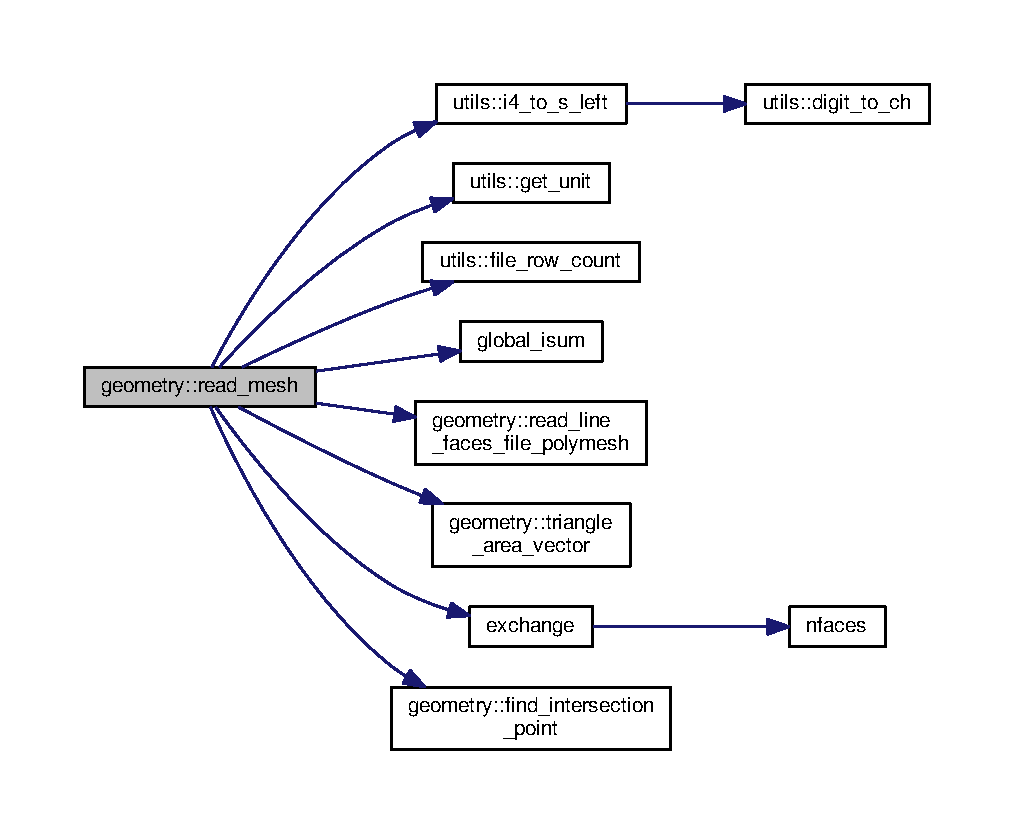
\includegraphics[width=350pt]{classgeometry_a6f11cfdf3b8f94b5dda77b3330f6428c_cgraph}
\end{center}
\end{figure}


\hypertarget{classgeometry_a5b97404630e45caf9cfe42e5986e1610}{\index{geometry@{geometry}!triangle\-\_\-area\-\_\-vector@{triangle\-\_\-area\-\_\-vector}}
\index{triangle\-\_\-area\-\_\-vector@{triangle\-\_\-area\-\_\-vector}!geometry@{geometry}}
\subsubsection[{triangle\-\_\-area\-\_\-vector}]{\setlength{\rightskip}{0pt plus 5cm}subroutine geometry\-::triangle\-\_\-area\-\_\-vector (
\begin{DoxyParamCaption}
\item[{real(dp), intent(in)}]{px, }
\item[{real(dp), intent(in)}]{py, }
\item[{real(dp), intent(in)}]{pz, }
\item[{real(dp), intent(in)}]{qx, }
\item[{real(dp), intent(in)}]{qy, }
\item[{real(dp), intent(in)}]{qz, }
\item[{real(dp), intent(inout)}]{nx, }
\item[{real(dp), intent(inout)}]{ny, }
\item[{real(dp), intent(inout)}]{nz}
\end{DoxyParamCaption}
)}}\label{classgeometry_a5b97404630e45caf9cfe42e5986e1610}


\subsection{Member Data Documentation}
\hypertarget{classgeometry_a471fde959c1d2bdc45facc53fae5fb5b}{\index{geometry@{geometry}!arx@{arx}}
\index{arx@{arx}!geometry@{geometry}}
\subsubsection[{arx}]{\setlength{\rightskip}{0pt plus 5cm}real(dp), dimension(\-:), allocatable geometry\-::arx}}\label{classgeometry_a471fde959c1d2bdc45facc53fae5fb5b}
\hypertarget{classgeometry_a20e05e2b4e25753dc0892a77029b94b8}{\index{geometry@{geometry}!ary@{ary}}
\index{ary@{ary}!geometry@{geometry}}
\subsubsection[{ary}]{\setlength{\rightskip}{0pt plus 5cm}real(dp), dimension(\-:), allocatable geometry\-::ary}}\label{classgeometry_a20e05e2b4e25753dc0892a77029b94b8}
\hypertarget{classgeometry_af05cbfe19f538092a328e02ba17ec1b9}{\index{geometry@{geometry}!arz@{arz}}
\index{arz@{arz}!geometry@{geometry}}
\subsubsection[{arz}]{\setlength{\rightskip}{0pt plus 5cm}real(dp), dimension(\-:), allocatable geometry\-::arz}}\label{classgeometry_af05cbfe19f538092a328e02ba17ec1b9}
\hypertarget{classgeometry_a4e43a18bec8fa1fa370aebdf28b26723}{\index{geometry@{geometry}!bcname@{bcname}}
\index{bcname@{bcname}!geometry@{geometry}}
\subsubsection[{bcname}]{\setlength{\rightskip}{0pt plus 5cm}character(len=15), dimension(\-:), allocatable geometry\-::bcname}}\label{classgeometry_a4e43a18bec8fa1fa370aebdf28b26723}
\hypertarget{classgeometry_a273882b8b9ef9670ecef4c22d7a1ffc3}{\index{geometry@{geometry}!bctype@{bctype}}
\index{bctype@{bctype}!geometry@{geometry}}
\subsubsection[{bctype}]{\setlength{\rightskip}{0pt plus 5cm}character(len=15), dimension(\-:), allocatable geometry\-::bctype}}\label{classgeometry_a273882b8b9ef9670ecef4c22d7a1ffc3}
\hypertarget{classgeometry_a7b1e102e0a1a96f15dcd1def8d7e0e28}{\index{geometry@{geometry}!boundary\-\_\-file@{boundary\-\_\-file}}
\index{boundary\-\_\-file@{boundary\-\_\-file}!geometry@{geometry}}
\subsubsection[{boundary\-\_\-file}]{\setlength{\rightskip}{0pt plus 5cm}integer geometry\-::boundary\-\_\-file}}\label{classgeometry_a7b1e102e0a1a96f15dcd1def8d7e0e28}
\hypertarget{classgeometry_a22e8c08158c2f0faf7a3ff6527281144}{\index{geometry@{geometry}!dns@{dns}}
\index{dns@{dns}!geometry@{geometry}}
\subsubsection[{dns}]{\setlength{\rightskip}{0pt plus 5cm}real(dp), dimension(\-:), allocatable geometry\-::dns}}\label{classgeometry_a22e8c08158c2f0faf7a3ff6527281144}
\hypertarget{classgeometry_a15d5598fc8fd8adf2a3a0218d2aef488}{\index{geometry@{geometry}!dnw@{dnw}}
\index{dnw@{dnw}!geometry@{geometry}}
\subsubsection[{dnw}]{\setlength{\rightskip}{0pt plus 5cm}real(dp), dimension(\-:), allocatable geometry\-::dnw}}\label{classgeometry_a15d5598fc8fd8adf2a3a0218d2aef488}
\hypertarget{classgeometry_af70942cfbb3d083b361d7c30d7c7d1b8}{\index{geometry@{geometry}!faces\-\_\-file@{faces\-\_\-file}}
\index{faces\-\_\-file@{faces\-\_\-file}!geometry@{geometry}}
\subsubsection[{faces\-\_\-file}]{\setlength{\rightskip}{0pt plus 5cm}integer geometry\-::faces\-\_\-file}}\label{classgeometry_af70942cfbb3d083b361d7c30d7c7d1b8}
\hypertarget{classgeometry_a637d800def3bd03fb7b696a0a31d23f6}{\index{geometry@{geometry}!facint@{facint}}
\index{facint@{facint}!geometry@{geometry}}
\subsubsection[{facint}]{\setlength{\rightskip}{0pt plus 5cm}real(dp), dimension(\-:), allocatable geometry\-::facint}}\label{classgeometry_a637d800def3bd03fb7b696a0a31d23f6}
\hypertarget{classgeometry_a992699ec16084d3f8cf7423b32fc02b6}{\index{geometry@{geometry}!fpro@{fpro}}
\index{fpro@{fpro}!geometry@{geometry}}
\subsubsection[{fpro}]{\setlength{\rightskip}{0pt plus 5cm}real(dp), dimension(\-:), allocatable geometry\-::fpro}}\label{classgeometry_a992699ec16084d3f8cf7423b32fc02b6}
\hypertarget{classgeometry_ad1e038213bb054d1e90870329c685f60}{\index{geometry@{geometry}!globfaces@{globfaces}}
\index{globfaces@{globfaces}!geometry@{geometry}}
\subsubsection[{globfaces}]{\setlength{\rightskip}{0pt plus 5cm}integer geometry\-::globfaces}}\label{classgeometry_ad1e038213bb054d1e90870329c685f60}
\hypertarget{classgeometry_a0512cb49b2ee4ae8aa67fe7b3e9cfa25}{\index{geometry@{geometry}!glocells@{glocells}}
\index{glocells@{glocells}!geometry@{geometry}}
\subsubsection[{glocells}]{\setlength{\rightskip}{0pt plus 5cm}integer geometry\-::glocells}}\label{classgeometry_a0512cb49b2ee4ae8aa67fe7b3e9cfa25}
\hypertarget{classgeometry_a11e0bee8bca796dfc9673a1652675d95}{\index{geometry@{geometry}!glofaces@{glofaces}}
\index{glofaces@{glofaces}!geometry@{geometry}}
\subsubsection[{glofaces}]{\setlength{\rightskip}{0pt plus 5cm}integer geometry\-::glofaces}}\label{classgeometry_a11e0bee8bca796dfc9673a1652675d95}
\hypertarget{classgeometry_aa0b3019664f1e20f95c082706fbf4bf6}{\index{geometry@{geometry}!gloifaces@{gloifaces}}
\index{gloifaces@{gloifaces}!geometry@{geometry}}
\subsubsection[{gloifaces}]{\setlength{\rightskip}{0pt plus 5cm}integer geometry\-::gloifaces}}\label{classgeometry_aa0b3019664f1e20f95c082706fbf4bf6}
\hypertarget{classgeometry_aa32cd7bcc888322cd384ba928fbe0fd8}{\index{geometry@{geometry}!glonodes@{glonodes}}
\index{glonodes@{glonodes}!geometry@{geometry}}
\subsubsection[{glonodes}]{\setlength{\rightskip}{0pt plus 5cm}integer geometry\-::glonodes}}\label{classgeometry_aa32cd7bcc888322cd384ba928fbe0fd8}
\hypertarget{classgeometry_ac725fa5c48485899cdc2607d4c0e3278}{\index{geometry@{geometry}!ibndvaluestart@{ibndvaluestart}}
\index{ibndvaluestart@{ibndvaluestart}!geometry@{geometry}}
\subsubsection[{ibndvaluestart}]{\setlength{\rightskip}{0pt plus 5cm}integer, dimension(\-:), allocatable geometry\-::ibndvaluestart}}\label{classgeometry_ac725fa5c48485899cdc2607d4c0e3278}
\hypertarget{classgeometry_afc765695937174a634f048738ae0dc8e}{\index{geometry@{geometry}!neighbour@{neighbour}}
\index{neighbour@{neighbour}!geometry@{geometry}}
\subsubsection[{neighbour}]{\setlength{\rightskip}{0pt plus 5cm}integer, dimension(\-:), allocatable geometry\-::neighbour}}\label{classgeometry_afc765695937174a634f048738ae0dc8e}
\hypertarget{classgeometry_a76fd3a715a134c4e338b1bef0d53563b}{\index{geometry@{geometry}!neighbour\-\_\-file@{neighbour\-\_\-file}}
\index{neighbour\-\_\-file@{neighbour\-\_\-file}!geometry@{geometry}}
\subsubsection[{neighbour\-\_\-file}]{\setlength{\rightskip}{0pt plus 5cm}integer geometry\-::neighbour\-\_\-file}}\label{classgeometry_a76fd3a715a134c4e338b1bef0d53563b}
\hypertarget{classgeometry_abc180e7f216d7319e972a77e754cf1ba}{\index{geometry@{geometry}!nfaces@{nfaces}}
\index{nfaces@{nfaces}!geometry@{geometry}}
\subsubsection[{nfaces}]{\setlength{\rightskip}{0pt plus 5cm}integer, dimension(\-:), allocatable geometry\-::nfaces}}\label{classgeometry_abc180e7f216d7319e972a77e754cf1ba}
\hypertarget{classgeometry_a7c3a12b979532a42fd4791cd336b388f}{\index{geometry@{geometry}!ninl@{ninl}}
\index{ninl@{ninl}!geometry@{geometry}}
\subsubsection[{ninl}]{\setlength{\rightskip}{0pt plus 5cm}integer geometry\-::ninl}}\label{classgeometry_a7c3a12b979532a42fd4791cd336b388f}
\hypertarget{classgeometry_aebf6156cf92933802643ed6612d80bcc}{\index{geometry@{geometry}!nomax@{nomax}}
\index{nomax@{nomax}!geometry@{geometry}}
\subsubsection[{nomax}]{\setlength{\rightskip}{0pt plus 5cm}integer, parameter geometry\-::nomax = 30}}\label{classgeometry_aebf6156cf92933802643ed6612d80bcc}
\hypertarget{classgeometry_af185a2e42ce8dc5f660f52f4e844d883}{\index{geometry@{geometry}!nout@{nout}}
\index{nout@{nout}!geometry@{geometry}}
\subsubsection[{nout}]{\setlength{\rightskip}{0pt plus 5cm}integer geometry\-::nout}}\label{classgeometry_af185a2e42ce8dc5f660f52f4e844d883}
\hypertarget{classgeometry_af9bcf0023987fb42899faea73e6e719d}{\index{geometry@{geometry}!npro@{npro}}
\index{npro@{npro}!geometry@{geometry}}
\subsubsection[{npro}]{\setlength{\rightskip}{0pt plus 5cm}integer geometry\-::npro}}\label{classgeometry_af9bcf0023987fb42899faea73e6e719d}
\hypertarget{classgeometry_a3267813953228bd94c67d73bd878eb9c}{\index{geometry@{geometry}!nsym@{nsym}}
\index{nsym@{nsym}!geometry@{geometry}}
\subsubsection[{nsym}]{\setlength{\rightskip}{0pt plus 5cm}integer geometry\-::nsym}}\label{classgeometry_a3267813953228bd94c67d73bd878eb9c}
\hypertarget{classgeometry_a18cc0b968a1496fa99a2ef47a0ee7d1a}{\index{geometry@{geometry}!numboundaries@{numboundaries}}
\index{numboundaries@{numboundaries}!geometry@{geometry}}
\subsubsection[{numboundaries}]{\setlength{\rightskip}{0pt plus 5cm}integer geometry\-::numboundaries}}\label{classgeometry_a18cc0b968a1496fa99a2ef47a0ee7d1a}
\hypertarget{classgeometry_aa40b31eef33895463f82107dec14911a}{\index{geometry@{geometry}!numboundaryfaces@{numboundaryfaces}}
\index{numboundaryfaces@{numboundaryfaces}!geometry@{geometry}}
\subsubsection[{numboundaryfaces}]{\setlength{\rightskip}{0pt plus 5cm}integer geometry\-::numboundaryfaces}}\label{classgeometry_aa40b31eef33895463f82107dec14911a}
\hypertarget{classgeometry_a6316b2c2a707e4250801749fad266b81}{\index{geometry@{geometry}!numcells@{numcells}}
\index{numcells@{numcells}!geometry@{geometry}}
\subsubsection[{numcells}]{\setlength{\rightskip}{0pt plus 5cm}integer geometry\-::numcells}}\label{classgeometry_a6316b2c2a707e4250801749fad266b81}
\hypertarget{classgeometry_a1fe23be4aa394d4647eb94f232ef7be4}{\index{geometry@{geometry}!numfaces@{numfaces}}
\index{numfaces@{numfaces}!geometry@{geometry}}
\subsubsection[{numfaces}]{\setlength{\rightskip}{0pt plus 5cm}integer geometry\-::numfaces}}\label{classgeometry_a1fe23be4aa394d4647eb94f232ef7be4}
\hypertarget{classgeometry_a3604c4b943618f96d25b4e57be2d730a}{\index{geometry@{geometry}!numinnerfaces@{numinnerfaces}}
\index{numinnerfaces@{numinnerfaces}!geometry@{geometry}}
\subsubsection[{numinnerfaces}]{\setlength{\rightskip}{0pt plus 5cm}integer geometry\-::numinnerfaces}}\label{classgeometry_a3604c4b943618f96d25b4e57be2d730a}
\hypertarget{classgeometry_a74e7aa9e5207d1bdf0ec33642daa1e95}{\index{geometry@{geometry}!numnodes@{numnodes}}
\index{numnodes@{numnodes}!geometry@{geometry}}
\subsubsection[{numnodes}]{\setlength{\rightskip}{0pt plus 5cm}integer geometry\-::numnodes}}\label{classgeometry_a74e7aa9e5207d1bdf0ec33642daa1e95}
\hypertarget{classgeometry_abe73a7c15a5676edffcb997de320903b}{\index{geometry@{geometry}!numpcells@{numpcells}}
\index{numpcells@{numpcells}!geometry@{geometry}}
\subsubsection[{numpcells}]{\setlength{\rightskip}{0pt plus 5cm}integer geometry\-::numpcells}}\label{classgeometry_abe73a7c15a5676edffcb997de320903b}
\hypertarget{classgeometry_a4b36c67fd5fbba66cd159331a6449464}{\index{geometry@{geometry}!numtotal@{numtotal}}
\index{numtotal@{numtotal}!geometry@{geometry}}
\subsubsection[{numtotal}]{\setlength{\rightskip}{0pt plus 5cm}integer geometry\-::numtotal}}\label{classgeometry_a4b36c67fd5fbba66cd159331a6449464}
\hypertarget{classgeometry_a3e083890c7aae9c07961696766208796}{\index{geometry@{geometry}!nwal@{nwal}}
\index{nwal@{nwal}!geometry@{geometry}}
\subsubsection[{nwal}]{\setlength{\rightskip}{0pt plus 5cm}integer geometry\-::nwal}}\label{classgeometry_a3e083890c7aae9c07961696766208796}
\hypertarget{classgeometry_ae59df205a86f69d3cc7ecf9917b3fc8d}{\index{geometry@{geometry}!owner@{owner}}
\index{owner@{owner}!geometry@{geometry}}
\subsubsection[{owner}]{\setlength{\rightskip}{0pt plus 5cm}integer, dimension(\-:), allocatable geometry\-::owner}}\label{classgeometry_ae59df205a86f69d3cc7ecf9917b3fc8d}
\hypertarget{classgeometry_aa4904f087664ad6358d283ca2e053b0f}{\index{geometry@{geometry}!owner\-\_\-file@{owner\-\_\-file}}
\index{owner\-\_\-file@{owner\-\_\-file}!geometry@{geometry}}
\subsubsection[{owner\-\_\-file}]{\setlength{\rightskip}{0pt plus 5cm}integer geometry\-::owner\-\_\-file}}\label{classgeometry_aa4904f087664ad6358d283ca2e053b0f}
\hypertarget{classgeometry_a4f9606dd6dec8a18282daf3096cd7074}{\index{geometry@{geometry}!points\-\_\-file@{points\-\_\-file}}
\index{points\-\_\-file@{points\-\_\-file}!geometry@{geometry}}
\subsubsection[{points\-\_\-file}]{\setlength{\rightskip}{0pt plus 5cm}integer geometry\-::points\-\_\-file}}\label{classgeometry_a4f9606dd6dec8a18282daf3096cd7074}
\hypertarget{classgeometry_a6d6c8b4ed2fdb31e8b906eccb7fe8bd2}{\index{geometry@{geometry}!process\-\_\-file@{process\-\_\-file}}
\index{process\-\_\-file@{process\-\_\-file}!geometry@{geometry}}
\subsubsection[{process\-\_\-file}]{\setlength{\rightskip}{0pt plus 5cm}integer geometry\-::process\-\_\-file}}\label{classgeometry_a6d6c8b4ed2fdb31e8b906eccb7fe8bd2}
\hypertarget{classgeometry_ad2388cd69f1b9efc5b4dafab1540e6fd}{\index{geometry@{geometry}!srds@{srds}}
\index{srds@{srds}!geometry@{geometry}}
\subsubsection[{srds}]{\setlength{\rightskip}{0pt plus 5cm}real(dp), dimension(\-:), allocatable geometry\-::srds}}\label{classgeometry_ad2388cd69f1b9efc5b4dafab1540e6fd}
\hypertarget{classgeometry_ad4f99f0dbd2866ccd6bb897c324fbbb9}{\index{geometry@{geometry}!srdw@{srdw}}
\index{srdw@{srdw}!geometry@{geometry}}
\subsubsection[{srdw}]{\setlength{\rightskip}{0pt plus 5cm}real(dp), dimension(\-:), allocatable geometry\-::srdw}}\label{classgeometry_ad4f99f0dbd2866ccd6bb897c324fbbb9}
\hypertarget{classgeometry_a18f4eb284c2fb036786e7cb078b1261b}{\index{geometry@{geometry}!startface@{startface}}
\index{startface@{startface}!geometry@{geometry}}
\subsubsection[{startface}]{\setlength{\rightskip}{0pt plus 5cm}integer, dimension(\-:), allocatable geometry\-::startface}}\label{classgeometry_a18f4eb284c2fb036786e7cb078b1261b}
\hypertarget{classgeometry_a8f9a710dae624d649ba6196d6a3ad819}{\index{geometry@{geometry}!tiny@{tiny}}
\index{tiny@{tiny}!geometry@{geometry}}
\subsubsection[{tiny}]{\setlength{\rightskip}{0pt plus 5cm}real(dp), parameter geometry\-::tiny = 1e-\/30}}\label{classgeometry_a8f9a710dae624d649ba6196d6a3ad819}
\hypertarget{classgeometry_a4d57310a2f6f4431e6ec39d9633b3cc5}{\index{geometry@{geometry}!vol@{vol}}
\index{vol@{vol}!geometry@{geometry}}
\subsubsection[{vol}]{\setlength{\rightskip}{0pt plus 5cm}real(dp), dimension(\-:), allocatable geometry\-::vol}}\label{classgeometry_a4d57310a2f6f4431e6ec39d9633b3cc5}
\hypertarget{classgeometry_a51893a5f373a1a6c12894eeb216ecc59}{\index{geometry@{geometry}!walldistance@{walldistance}}
\index{walldistance@{walldistance}!geometry@{geometry}}
\subsubsection[{walldistance}]{\setlength{\rightskip}{0pt plus 5cm}real(dp), dimension(\-:), allocatable geometry\-::walldistance}}\label{classgeometry_a51893a5f373a1a6c12894eeb216ecc59}
\hypertarget{classgeometry_addb7458352afb3060d5831f54b39ca61}{\index{geometry@{geometry}!x@{x}}
\index{x@{x}!geometry@{geometry}}
\subsubsection[{x}]{\setlength{\rightskip}{0pt plus 5cm}real(dp), dimension(\-:), allocatable geometry\-::x}}\label{classgeometry_addb7458352afb3060d5831f54b39ca61}
\hypertarget{classgeometry_ab8a1629eea878ff62c7dbd6b6025fc55}{\index{geometry@{geometry}!xc@{xc}}
\index{xc@{xc}!geometry@{geometry}}
\subsubsection[{xc}]{\setlength{\rightskip}{0pt plus 5cm}real(dp), dimension(\-:), allocatable geometry\-::xc}}\label{classgeometry_ab8a1629eea878ff62c7dbd6b6025fc55}
\hypertarget{classgeometry_a6be1b0f6e7647b5eea5975c28be87ba3}{\index{geometry@{geometry}!xf@{xf}}
\index{xf@{xf}!geometry@{geometry}}
\subsubsection[{xf}]{\setlength{\rightskip}{0pt plus 5cm}real(dp), dimension(\-:), allocatable geometry\-::xf}}\label{classgeometry_a6be1b0f6e7647b5eea5975c28be87ba3}
\hypertarget{classgeometry_afd0076c8984ed089741c40a24b176665}{\index{geometry@{geometry}!xnp@{xnp}}
\index{xnp@{xnp}!geometry@{geometry}}
\subsubsection[{xnp}]{\setlength{\rightskip}{0pt plus 5cm}real(dp), dimension(\-:), allocatable geometry\-::xnp}}\label{classgeometry_afd0076c8984ed089741c40a24b176665}
\hypertarget{classgeometry_adb87ebbb8b31be2d1372108e5057ab11}{\index{geometry@{geometry}!xpp@{xpp}}
\index{xpp@{xpp}!geometry@{geometry}}
\subsubsection[{xpp}]{\setlength{\rightskip}{0pt plus 5cm}real(dp), dimension(\-:), allocatable geometry\-::xpp}}\label{classgeometry_adb87ebbb8b31be2d1372108e5057ab11}
\hypertarget{classgeometry_a12fdb27cf84ec561b9c20625748e8f57}{\index{geometry@{geometry}!y@{y}}
\index{y@{y}!geometry@{geometry}}
\subsubsection[{y}]{\setlength{\rightskip}{0pt plus 5cm}real(dp), dimension(\-:), allocatable geometry\-::y}}\label{classgeometry_a12fdb27cf84ec561b9c20625748e8f57}
\hypertarget{classgeometry_a23fc04ce2affc5bb7f3b1f3464feab40}{\index{geometry@{geometry}!yc@{yc}}
\index{yc@{yc}!geometry@{geometry}}
\subsubsection[{yc}]{\setlength{\rightskip}{0pt plus 5cm}real(dp), dimension(\-:), allocatable geometry\-::yc}}\label{classgeometry_a23fc04ce2affc5bb7f3b1f3464feab40}
\hypertarget{classgeometry_a6f897e422e91f75c528d0c855a933271}{\index{geometry@{geometry}!yf@{yf}}
\index{yf@{yf}!geometry@{geometry}}
\subsubsection[{yf}]{\setlength{\rightskip}{0pt plus 5cm}real(dp), dimension(\-:), allocatable geometry\-::yf}}\label{classgeometry_a6f897e422e91f75c528d0c855a933271}
\hypertarget{classgeometry_a2fd843e613749c67542f4377ed724ef9}{\index{geometry@{geometry}!ynp@{ynp}}
\index{ynp@{ynp}!geometry@{geometry}}
\subsubsection[{ynp}]{\setlength{\rightskip}{0pt plus 5cm}real(dp), dimension(\-:), allocatable geometry\-::ynp}}\label{classgeometry_a2fd843e613749c67542f4377ed724ef9}
\hypertarget{classgeometry_a0e0c8bc792d7ff52c12df810cb39bde6}{\index{geometry@{geometry}!ypp@{ypp}}
\index{ypp@{ypp}!geometry@{geometry}}
\subsubsection[{ypp}]{\setlength{\rightskip}{0pt plus 5cm}real(dp), dimension(\-:), allocatable geometry\-::ypp}}\label{classgeometry_a0e0c8bc792d7ff52c12df810cb39bde6}
\hypertarget{classgeometry_a567da85e335951f534f57b51765df56a}{\index{geometry@{geometry}!z@{z}}
\index{z@{z}!geometry@{geometry}}
\subsubsection[{z}]{\setlength{\rightskip}{0pt plus 5cm}real(dp), dimension(\-:), allocatable geometry\-::z}}\label{classgeometry_a567da85e335951f534f57b51765df56a}
\hypertarget{classgeometry_accaf072ca71c8cf746b911dfc0165664}{\index{geometry@{geometry}!zc@{zc}}
\index{zc@{zc}!geometry@{geometry}}
\subsubsection[{zc}]{\setlength{\rightskip}{0pt plus 5cm}real(dp), dimension(\-:), allocatable geometry\-::zc}}\label{classgeometry_accaf072ca71c8cf746b911dfc0165664}
\hypertarget{classgeometry_acf0149de3e29b6714898a4db86b62435}{\index{geometry@{geometry}!zf@{zf}}
\index{zf@{zf}!geometry@{geometry}}
\subsubsection[{zf}]{\setlength{\rightskip}{0pt plus 5cm}real(dp), dimension(\-:), allocatable geometry\-::zf}}\label{classgeometry_acf0149de3e29b6714898a4db86b62435}
\hypertarget{classgeometry_a40f59df46474b424b2545f108ac317ec}{\index{geometry@{geometry}!znp@{znp}}
\index{znp@{znp}!geometry@{geometry}}
\subsubsection[{znp}]{\setlength{\rightskip}{0pt plus 5cm}real(dp), dimension(\-:), allocatable geometry\-::znp}}\label{classgeometry_a40f59df46474b424b2545f108ac317ec}
\hypertarget{classgeometry_a55be35632eac8306e28a7d900e1c9cb1}{\index{geometry@{geometry}!zpp@{zpp}}
\index{zpp@{zpp}!geometry@{geometry}}
\subsubsection[{zpp}]{\setlength{\rightskip}{0pt plus 5cm}real(dp), dimension(\-:), allocatable geometry\-::zpp}}\label{classgeometry_a55be35632eac8306e28a7d900e1c9cb1}


The documentation for this module was generated from the following file\-:\begin{DoxyCompactItemize}
\item 
src-\/par/\hyperlink{geometry_8f90}{geometry.\-f90}\end{DoxyCompactItemize}

\hypertarget{interfacegradients_1_1grad}{\section{gradients\-:\-:grad Interface Reference}
\label{interfacegradients_1_1grad}\index{gradients\-::grad@{gradients\-::grad}}
}
\subsection*{Public Member Functions}
\begin{DoxyCompactItemize}
\item 
subroutine \hyperlink{interfacegradients_1_1grad_a5cf477680ba1663dd2a19fca4667393d}{grad\-\_\-scalar\-\_\-field} (phi, d\-Phidxi)
\item 
subroutine \hyperlink{interfacegradients_1_1grad_a10bfb0c5c2ca801765cb5cf1826ab634}{grad\-\_\-vector\-\_\-field} (U, V, W, d\-Udxi, d\-Vdxi, d\-Wdxi)
\item 
subroutine \hyperlink{interfacegradients_1_1grad_ad9be9824ec8b3b537c0b501967f241a8}{grad\-\_\-scalar\-\_\-field\-\_\-w\-\_\-option} (phi, d\-Phidxi, option, option\-\_\-limiter)
\end{DoxyCompactItemize}


\subsection{Member Function/\-Subroutine Documentation}
\hypertarget{interfacegradients_1_1grad_a5cf477680ba1663dd2a19fca4667393d}{\index{gradients\-::grad@{gradients\-::grad}!grad\-\_\-scalar\-\_\-field@{grad\-\_\-scalar\-\_\-field}}
\index{grad\-\_\-scalar\-\_\-field@{grad\-\_\-scalar\-\_\-field}!gradients::grad@{gradients\-::grad}}
\subsubsection[{grad\-\_\-scalar\-\_\-field}]{\setlength{\rightskip}{0pt plus 5cm}subroutine gradients\-::grad\-::grad\-\_\-scalar\-\_\-field (
\begin{DoxyParamCaption}
\item[{real(dp), dimension(numtotal), intent(inout)}]{phi, }
\item[{real(dp), dimension(3,numtotal), intent(inout)}]{d\-Phidxi}
\end{DoxyParamCaption}
)}}\label{interfacegradients_1_1grad_a5cf477680ba1663dd2a19fca4667393d}
\hypertarget{interfacegradients_1_1grad_ad9be9824ec8b3b537c0b501967f241a8}{\index{gradients\-::grad@{gradients\-::grad}!grad\-\_\-scalar\-\_\-field\-\_\-w\-\_\-option@{grad\-\_\-scalar\-\_\-field\-\_\-w\-\_\-option}}
\index{grad\-\_\-scalar\-\_\-field\-\_\-w\-\_\-option@{grad\-\_\-scalar\-\_\-field\-\_\-w\-\_\-option}!gradients::grad@{gradients\-::grad}}
\subsubsection[{grad\-\_\-scalar\-\_\-field\-\_\-w\-\_\-option}]{\setlength{\rightskip}{0pt plus 5cm}subroutine gradients\-::grad\-::grad\-\_\-scalar\-\_\-field\-\_\-w\-\_\-option (
\begin{DoxyParamCaption}
\item[{real(dp), dimension(numtotal), intent(in)}]{phi, }
\item[{real(dp), dimension(3,numtotal), intent(inout)}]{d\-Phidxi, }
\item[{character( len=$\ast$ ), intent(in)}]{option, }
\item[{character( len=$\ast$ ), intent(in)}]{option\-\_\-limiter}
\end{DoxyParamCaption}
)}}\label{interfacegradients_1_1grad_ad9be9824ec8b3b537c0b501967f241a8}
\hypertarget{interfacegradients_1_1grad_a10bfb0c5c2ca801765cb5cf1826ab634}{\index{gradients\-::grad@{gradients\-::grad}!grad\-\_\-vector\-\_\-field@{grad\-\_\-vector\-\_\-field}}
\index{grad\-\_\-vector\-\_\-field@{grad\-\_\-vector\-\_\-field}!gradients::grad@{gradients\-::grad}}
\subsubsection[{grad\-\_\-vector\-\_\-field}]{\setlength{\rightskip}{0pt plus 5cm}subroutine gradients\-::grad\-::grad\-\_\-vector\-\_\-field (
\begin{DoxyParamCaption}
\item[{real(dp), dimension(numtotal), intent(inout)}]{U, }
\item[{real(dp), dimension(numtotal), intent(inout)}]{V, }
\item[{real(dp), dimension(numtotal), intent(inout)}]{W, }
\item[{real(dp), dimension(3,numtotal), intent(inout)}]{d\-Udxi, }
\item[{real(dp), dimension(3,numtotal), intent(inout)}]{d\-Vdxi, }
\item[{real(dp), dimension(3,numtotal), intent(inout)}]{d\-Wdxi}
\end{DoxyParamCaption}
)}}\label{interfacegradients_1_1grad_a10bfb0c5c2ca801765cb5cf1826ab634}


The documentation for this interface was generated from the following file\-:\begin{DoxyCompactItemize}
\item 
src-\/par/\hyperlink{gradients_8f90}{gradients.\-f90}\end{DoxyCompactItemize}

\hypertarget{classgradients}{\section{gradients Module Reference}
\label{classgradients}\index{gradients@{gradients}}
}
\subsection*{Data Types}
\begin{DoxyCompactItemize}
\item 
interface \hyperlink{interfacegradients_1_1grad}{grad}
\item 
interface \hyperlink{interfacegradients_1_1sngrad}{sngrad}
\end{DoxyCompactItemize}
\subsection*{Public Member Functions}
\begin{DoxyCompactItemize}
\item 
subroutine, public \hyperlink{classgradients_a89f491e7b33a1042b176ce9cbf6cbea7}{create\-\_\-lsq\-\_\-grad\-\_\-matrix} (phi, d\-Phidxi)
\item 
subroutine \hyperlink{classgradients_af8d86227570d2a05536bc966c46f3fef}{slope\-\_\-limiter\-\_\-modified\-\_\-venkatakrishnan} (phi, d\-Phidxi)
\item 
subroutine \hyperlink{classgradients_ab7860442796eb435f5c34667b8c7c008}{slope\-\_\-limiter\-\_\-barth\-\_\-jespersen} (phi, d\-Phidxi)
\item 
subroutine \hyperlink{classgradients_a524feb6c9302fc86d0189ad33cf7485c}{grad\-\_\-lsq\-\_\-qr} (fi, dfidxi, istage, d)
\item 
subroutine \hyperlink{classgradients_abf08289bb8d57d8177f75a1028008906}{grad\-\_\-lsq\-\_\-dm} (fi, d\-Fidxi, istage, \hyperlink{classgradients_a0417bd090ffd38c01cbcc0d76068dd82}{dmat})
\item 
subroutine \hyperlink{classgradients_a79da9651b35bd925b488cb7cff3abb7f}{grad\-\_\-gauss} (u, dudx, dudy, dudz)
\item 
subroutine \hyperlink{classgradients_a01a46b4478e35c25121d4ad506c757fc}{grad\-\_\-gauss\-\_\-corrected} (u, dudx, dudy, dudz)
\item 
subroutine \hyperlink{classgradients_a437864d9f0535f851ceb4272b256f4ea}{gradco} (\hyperlink{CourantNo_8h_accea320a458bb8759c7ece360e05ddf4}{ijp}, ijn, xfc, yfc, zfc, sx, sy, sz, fif, fi, dfxo, dfyo, dfzo, dfx, dfy, dfz)
\item 
subroutine \hyperlink{classgradients_a95333310c398e2b695c12e0d388000d9}{gradcopar} (\hyperlink{CourantNo_8h_accea320a458bb8759c7ece360e05ddf4}{ijp}, ijn, ijnp, xfc, yfc, zfc, sx, sy, sz, fif, fi, dfxo, dfyo, dfzo, dfx, dfy, dfz)
\item 
subroutine \hyperlink{classgradients_abd2236c107f7c7c31c3f7fb638bb7b21}{gradbc} (sx, sy, sz, fi, dfx, dfy, dfz)
\item 
subroutine \hyperlink{classgradients_adcec95a6cfc9fbeb540b8a4a457bb2c6}{sngrad\-\_\-scalar\-\_\-field} (\hyperlink{CourantNo_8h_accea320a458bb8759c7ece360e05ddf4}{ijp}, ijn, xf, yf, zf, arx, ary, arz, lambda, Fi, d\-Fidxi, nrelax, approach, dfixi, dfiyi, dfizi, dfixii, dfiyii, dfizii)
\end{DoxyCompactItemize}
\subsection*{Public Attributes}
\begin{DoxyCompactItemize}
\item 
logical, public \hyperlink{classgradients_a4ef80ad8cc52782050167ed49c332c1e}{lstsq}
\item 
logical, public \hyperlink{classgradients_ae25a8c84c0815435812f94b82d7dafb7}{lstsq\-\_\-qr}
\item 
logical, public \hyperlink{classgradients_a65547c6133cbc486266ac66604342516}{lstsq\-\_\-dm}
\item 
logical, public \hyperlink{classgradients_ac41921915930ac80ed01373fd760ac51}{gauss}
\item 
character(len=20), public \hyperlink{classgradients_a47d37226aa24f4261a63b5cb1fa3d17c}{limiter}
\item 
character(len=12), public \hyperlink{classgradients_ae02e791dcca067360cb4c1802dd6ef8d}{sngrad\-\_\-corr}
\item 
real(dp), dimension(\-:,\-:), \\*
allocatable, save \hyperlink{classgradients_a0417bd090ffd38c01cbcc0d76068dd82}{dmat}
\item 
real(dp), dimension(\-:,\-:,\-:), \\*
allocatable \hyperlink{classgradients_a916054df6a0aaa257f536e0ef098b188}{dmatqr}
\end{DoxyCompactItemize}
\subsection*{Private Member Functions}
\begin{DoxyCompactItemize}
\item 
subroutine \hyperlink{classgradients_a74c0ecdda1ac9d450a0a6538359a6f11}{allocate\-\_\-lsq\-\_\-grad\-\_\-matrix}
\item 
subroutine \hyperlink{classgradients_a52798a9b8eaa888cb6254351a92386ef}{grad\-\_\-scalar\-\_\-field} (phi, d\-Phidxi)
\item 
subroutine \hyperlink{classgradients_a1cb60b38f23f9eb2ee50d537db912cfc}{grad\-\_\-vector\-\_\-field} (U, V, W, d\-Udxi, d\-Vdxi, d\-Wdxi)
\item 
subroutine \hyperlink{classgradients_a12593273fc9f5b56e9ddcad0f8945fa7}{grad\-\_\-scalar\-\_\-field\-\_\-w\-\_\-option} (phi, d\-Phidxi, option, option\-\_\-limiter)
\item 
subroutine \hyperlink{classgradients_af5ae74b1fab366ce3167820e0c6c5c3d}{set\-\_\-phi\-\_\-min\-\_\-max} (phi)
\item 
subroutine \hyperlink{classgradients_a19b76f98ae2657d4f6c3710bd2d8d0be}{slope\-\_\-limiter\-\_\-venkatakrishnan} (phi, d\-Phidxi)
\item 
subroutine \hyperlink{classgradients_a5392f6682ac037eae87dbe5f20d1205f}{slope\-\_\-limiter\-\_\-multidimensional} (phi, d\-Phidxi)
\item 
subroutine \hyperlink{classgradients_a38bb77fa9833da1c198aac2e7ea7c946}{grad\-\_\-lsq} (fi, d\-Fidxi, istage, \hyperlink{classgradients_a0417bd090ffd38c01cbcc0d76068dd82}{dmat})
\item 
subroutine \hyperlink{classgradients_a85591b848f22ed6fefebedf8f90e9246}{sngrad\-\_\-vector\-\_\-field} (\hyperlink{CourantNo_8h_accea320a458bb8759c7ece360e05ddf4}{ijp}, ijn, xf, yf, zf, arx, ary, arz, lambda, u, v, w, dudxi, dvdxi, dwdxi, nrelax, approach, duxi, duyi, duzi, dvxi, dvyi, dvzi, dwxi, dwyi, dwzi, duxii, dvxii, dwxii, duyii, dvyii, dwyii, duzii, dvzii, dwzii)
\end{DoxyCompactItemize}


\subsection{Member Function/\-Subroutine Documentation}
\hypertarget{classgradients_a74c0ecdda1ac9d450a0a6538359a6f11}{\index{gradients@{gradients}!allocate\-\_\-lsq\-\_\-grad\-\_\-matrix@{allocate\-\_\-lsq\-\_\-grad\-\_\-matrix}}
\index{allocate\-\_\-lsq\-\_\-grad\-\_\-matrix@{allocate\-\_\-lsq\-\_\-grad\-\_\-matrix}!gradients@{gradients}}
\subsubsection[{allocate\-\_\-lsq\-\_\-grad\-\_\-matrix}]{\setlength{\rightskip}{0pt plus 5cm}subroutine gradients\-::allocate\-\_\-lsq\-\_\-grad\-\_\-matrix (
\begin{DoxyParamCaption}
{}
\end{DoxyParamCaption}
)\hspace{0.3cm}{\ttfamily [private]}}}\label{classgradients_a74c0ecdda1ac9d450a0a6538359a6f11}
\hypertarget{classgradients_a89f491e7b33a1042b176ce9cbf6cbea7}{\index{gradients@{gradients}!create\-\_\-lsq\-\_\-grad\-\_\-matrix@{create\-\_\-lsq\-\_\-grad\-\_\-matrix}}
\index{create\-\_\-lsq\-\_\-grad\-\_\-matrix@{create\-\_\-lsq\-\_\-grad\-\_\-matrix}!gradients@{gradients}}
\subsubsection[{create\-\_\-lsq\-\_\-grad\-\_\-matrix}]{\setlength{\rightskip}{0pt plus 5cm}subroutine, public gradients\-::create\-\_\-lsq\-\_\-grad\-\_\-matrix (
\begin{DoxyParamCaption}
\item[{real(dp), dimension(numtotal), intent(in)}]{phi, }
\item[{real(dp), dimension(3,numcells), intent(inout)}]{d\-Phidxi}
\end{DoxyParamCaption}
)}}\label{classgradients_a89f491e7b33a1042b176ce9cbf6cbea7}


Here is the call graph for this function\-:\nopagebreak
\begin{figure}[H]
\begin{center}
\leavevmode
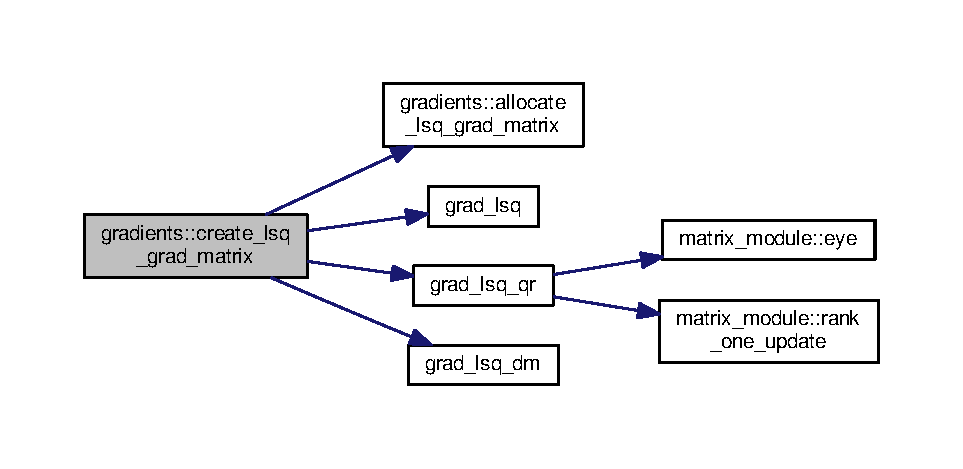
\includegraphics[width=350pt]{classgradients_a89f491e7b33a1042b176ce9cbf6cbea7_cgraph}
\end{center}
\end{figure}


\hypertarget{classgradients_a79da9651b35bd925b488cb7cff3abb7f}{\index{gradients@{gradients}!grad\-\_\-gauss@{grad\-\_\-gauss}}
\index{grad\-\_\-gauss@{grad\-\_\-gauss}!gradients@{gradients}}
\subsubsection[{grad\-\_\-gauss}]{\setlength{\rightskip}{0pt plus 5cm}subroutine gradients\-::grad\-\_\-gauss (
\begin{DoxyParamCaption}
\item[{real(dp), dimension(numtotal), intent(in)}]{u, }
\item[{real(dp), dimension(numcells), intent(inout)}]{dudx, }
\item[{real(dp), dimension(numcells), intent(inout)}]{dudy, }
\item[{real(dp), dimension(numcells), intent(inout)}]{dudz}
\end{DoxyParamCaption}
)}}\label{classgradients_a79da9651b35bd925b488cb7cff3abb7f}


Here is the call graph for this function\-:\nopagebreak
\begin{figure}[H]
\begin{center}
\leavevmode
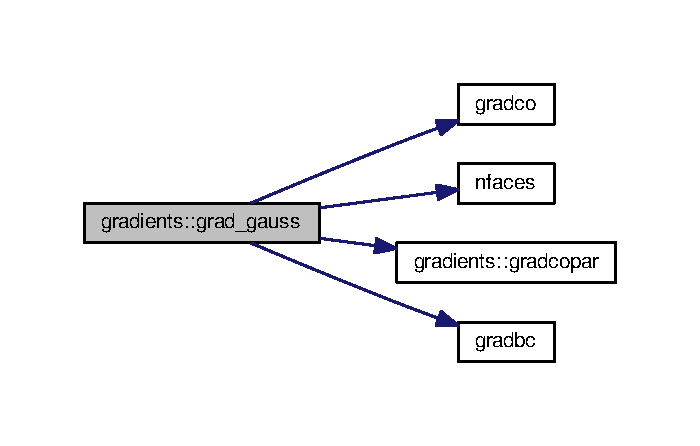
\includegraphics[width=336pt]{classgradients_a79da9651b35bd925b488cb7cff3abb7f_cgraph}
\end{center}
\end{figure}


\hypertarget{classgradients_a01a46b4478e35c25121d4ad506c757fc}{\index{gradients@{gradients}!grad\-\_\-gauss\-\_\-corrected@{grad\-\_\-gauss\-\_\-corrected}}
\index{grad\-\_\-gauss\-\_\-corrected@{grad\-\_\-gauss\-\_\-corrected}!gradients@{gradients}}
\subsubsection[{grad\-\_\-gauss\-\_\-corrected}]{\setlength{\rightskip}{0pt plus 5cm}subroutine gradients\-::grad\-\_\-gauss\-\_\-corrected (
\begin{DoxyParamCaption}
\item[{real(dp), dimension(numtotal), intent(in)}]{u, }
\item[{real(dp), dimension(numcells), intent(inout)}]{dudx, }
\item[{real(dp), dimension(numcells), intent(inout)}]{dudy, }
\item[{real(dp), dimension(numcells), intent(inout)}]{dudz}
\end{DoxyParamCaption}
)}}\label{classgradients_a01a46b4478e35c25121d4ad506c757fc}


Here is the call graph for this function\-:\nopagebreak
\begin{figure}[H]
\begin{center}
\leavevmode
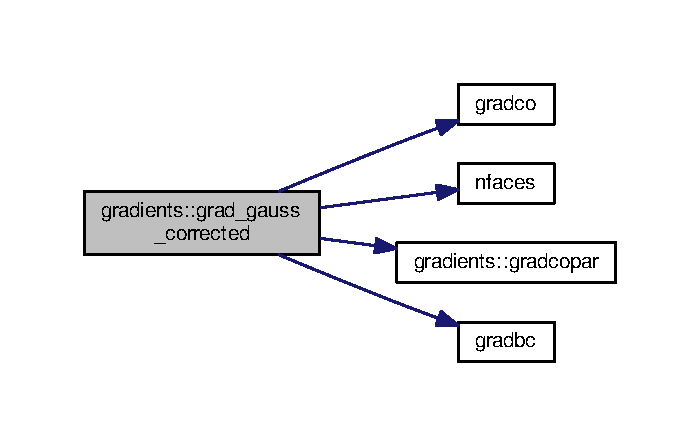
\includegraphics[width=336pt]{classgradients_a01a46b4478e35c25121d4ad506c757fc_cgraph}
\end{center}
\end{figure}


\hypertarget{classgradients_a38bb77fa9833da1c198aac2e7ea7c946}{\index{gradients@{gradients}!grad\-\_\-lsq@{grad\-\_\-lsq}}
\index{grad\-\_\-lsq@{grad\-\_\-lsq}!gradients@{gradients}}
\subsubsection[{grad\-\_\-lsq}]{\setlength{\rightskip}{0pt plus 5cm}subroutine gradients\-::grad\-\_\-lsq (
\begin{DoxyParamCaption}
\item[{real(dp), dimension(numtotal), intent(in)}]{fi, }
\item[{real(dp), dimension(3,numcells), intent(inout)}]{d\-Fidxi, }
\item[{integer, intent(in)}]{istage, }
\item[{real(dp), dimension(9,numcells), intent(inout)}]{dmat}
\end{DoxyParamCaption}
)\hspace{0.3cm}{\ttfamily [private]}}}\label{classgradients_a38bb77fa9833da1c198aac2e7ea7c946}


Here is the call graph for this function\-:\nopagebreak
\begin{figure}[H]
\begin{center}
\leavevmode
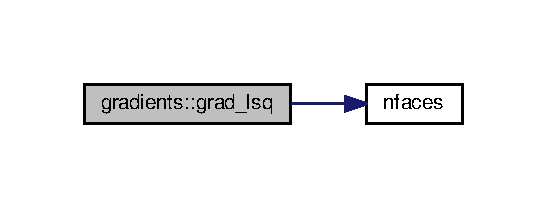
\includegraphics[width=262pt]{classgradients_a38bb77fa9833da1c198aac2e7ea7c946_cgraph}
\end{center}
\end{figure}


\hypertarget{classgradients_abf08289bb8d57d8177f75a1028008906}{\index{gradients@{gradients}!grad\-\_\-lsq\-\_\-dm@{grad\-\_\-lsq\-\_\-dm}}
\index{grad\-\_\-lsq\-\_\-dm@{grad\-\_\-lsq\-\_\-dm}!gradients@{gradients}}
\subsubsection[{grad\-\_\-lsq\-\_\-dm}]{\setlength{\rightskip}{0pt plus 5cm}subroutine gradients\-::grad\-\_\-lsq\-\_\-dm (
\begin{DoxyParamCaption}
\item[{real(dp), dimension(numtotal), intent(in)}]{fi, }
\item[{real(dp), dimension(3,numcells), intent(inout)}]{d\-Fidxi, }
\item[{integer, intent(in)}]{istage, }
\item[{real(dp), dimension(9,numcells), intent(inout)}]{dmat}
\end{DoxyParamCaption}
)}}\label{classgradients_abf08289bb8d57d8177f75a1028008906}


Here is the call graph for this function\-:\nopagebreak
\begin{figure}[H]
\begin{center}
\leavevmode
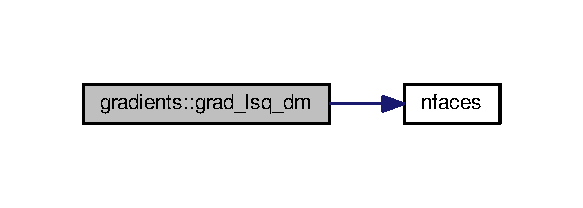
\includegraphics[width=280pt]{classgradients_abf08289bb8d57d8177f75a1028008906_cgraph}
\end{center}
\end{figure}


\hypertarget{classgradients_a524feb6c9302fc86d0189ad33cf7485c}{\index{gradients@{gradients}!grad\-\_\-lsq\-\_\-qr@{grad\-\_\-lsq\-\_\-qr}}
\index{grad\-\_\-lsq\-\_\-qr@{grad\-\_\-lsq\-\_\-qr}!gradients@{gradients}}
\subsubsection[{grad\-\_\-lsq\-\_\-qr}]{\setlength{\rightskip}{0pt plus 5cm}subroutine gradients\-::grad\-\_\-lsq\-\_\-qr (
\begin{DoxyParamCaption}
\item[{real(dp), dimension(numtotal), intent(in)}]{fi, }
\item[{real(dp), dimension(n,numcells), intent(inout)}]{dfidxi, }
\item[{integer, intent(in)}]{istage, }
\item[{real(dp), dimension(n,m,numcells), intent(inout)}]{d}
\end{DoxyParamCaption}
)}}\label{classgradients_a524feb6c9302fc86d0189ad33cf7485c}


Here is the call graph for this function\-:\nopagebreak
\begin{figure}[H]
\begin{center}
\leavevmode
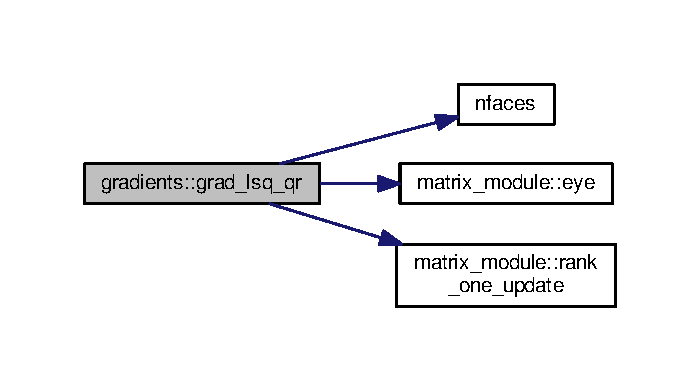
\includegraphics[width=336pt]{classgradients_a524feb6c9302fc86d0189ad33cf7485c_cgraph}
\end{center}
\end{figure}


\hypertarget{classgradients_a52798a9b8eaa888cb6254351a92386ef}{\index{gradients@{gradients}!grad\-\_\-scalar\-\_\-field@{grad\-\_\-scalar\-\_\-field}}
\index{grad\-\_\-scalar\-\_\-field@{grad\-\_\-scalar\-\_\-field}!gradients@{gradients}}
\subsubsection[{grad\-\_\-scalar\-\_\-field}]{\setlength{\rightskip}{0pt plus 5cm}subroutine gradients\-::grad\-\_\-scalar\-\_\-field (
\begin{DoxyParamCaption}
\item[{real(dp), dimension(numtotal), intent(inout)}]{phi, }
\item[{real(dp), dimension(3,numtotal), intent(inout)}]{d\-Phidxi}
\end{DoxyParamCaption}
)\hspace{0.3cm}{\ttfamily [private]}}}\label{classgradients_a52798a9b8eaa888cb6254351a92386ef}


Here is the call graph for this function\-:\nopagebreak
\begin{figure}[H]
\begin{center}
\leavevmode
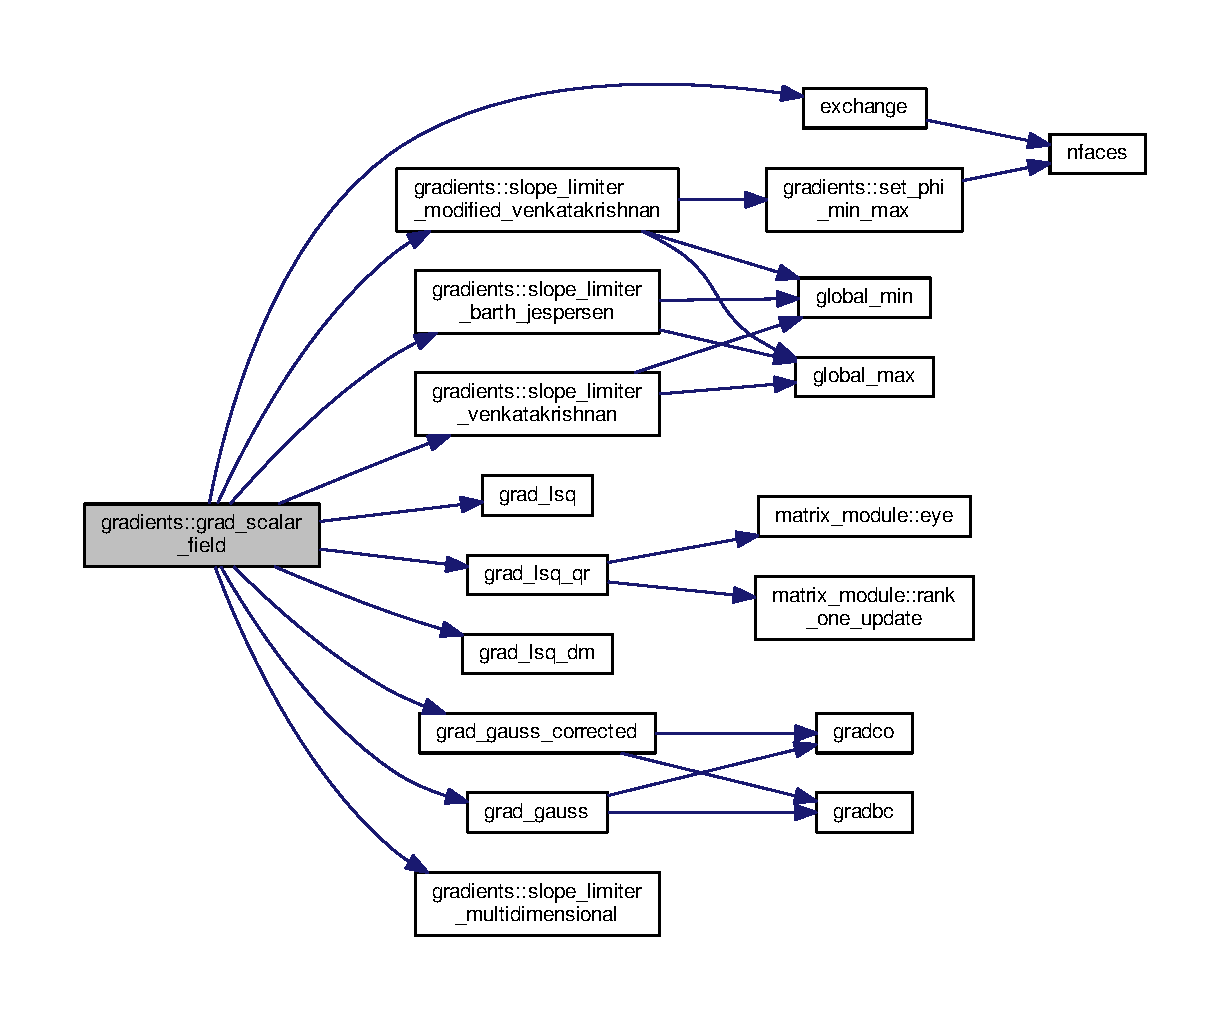
\includegraphics[width=350pt]{classgradients_a52798a9b8eaa888cb6254351a92386ef_cgraph}
\end{center}
\end{figure}


\hypertarget{classgradients_a12593273fc9f5b56e9ddcad0f8945fa7}{\index{gradients@{gradients}!grad\-\_\-scalar\-\_\-field\-\_\-w\-\_\-option@{grad\-\_\-scalar\-\_\-field\-\_\-w\-\_\-option}}
\index{grad\-\_\-scalar\-\_\-field\-\_\-w\-\_\-option@{grad\-\_\-scalar\-\_\-field\-\_\-w\-\_\-option}!gradients@{gradients}}
\subsubsection[{grad\-\_\-scalar\-\_\-field\-\_\-w\-\_\-option}]{\setlength{\rightskip}{0pt plus 5cm}subroutine gradients\-::grad\-\_\-scalar\-\_\-field\-\_\-w\-\_\-option (
\begin{DoxyParamCaption}
\item[{real(dp), dimension(numtotal), intent(in)}]{phi, }
\item[{real(dp), dimension(3,numtotal), intent(inout)}]{d\-Phidxi, }
\item[{character( len=$\ast$ ), intent(in)}]{option, }
\item[{character( len=$\ast$ ), intent(in)}]{option\-\_\-limiter}
\end{DoxyParamCaption}
)\hspace{0.3cm}{\ttfamily [private]}}}\label{classgradients_a12593273fc9f5b56e9ddcad0f8945fa7}


Here is the call graph for this function\-:\nopagebreak
\begin{figure}[H]
\begin{center}
\leavevmode
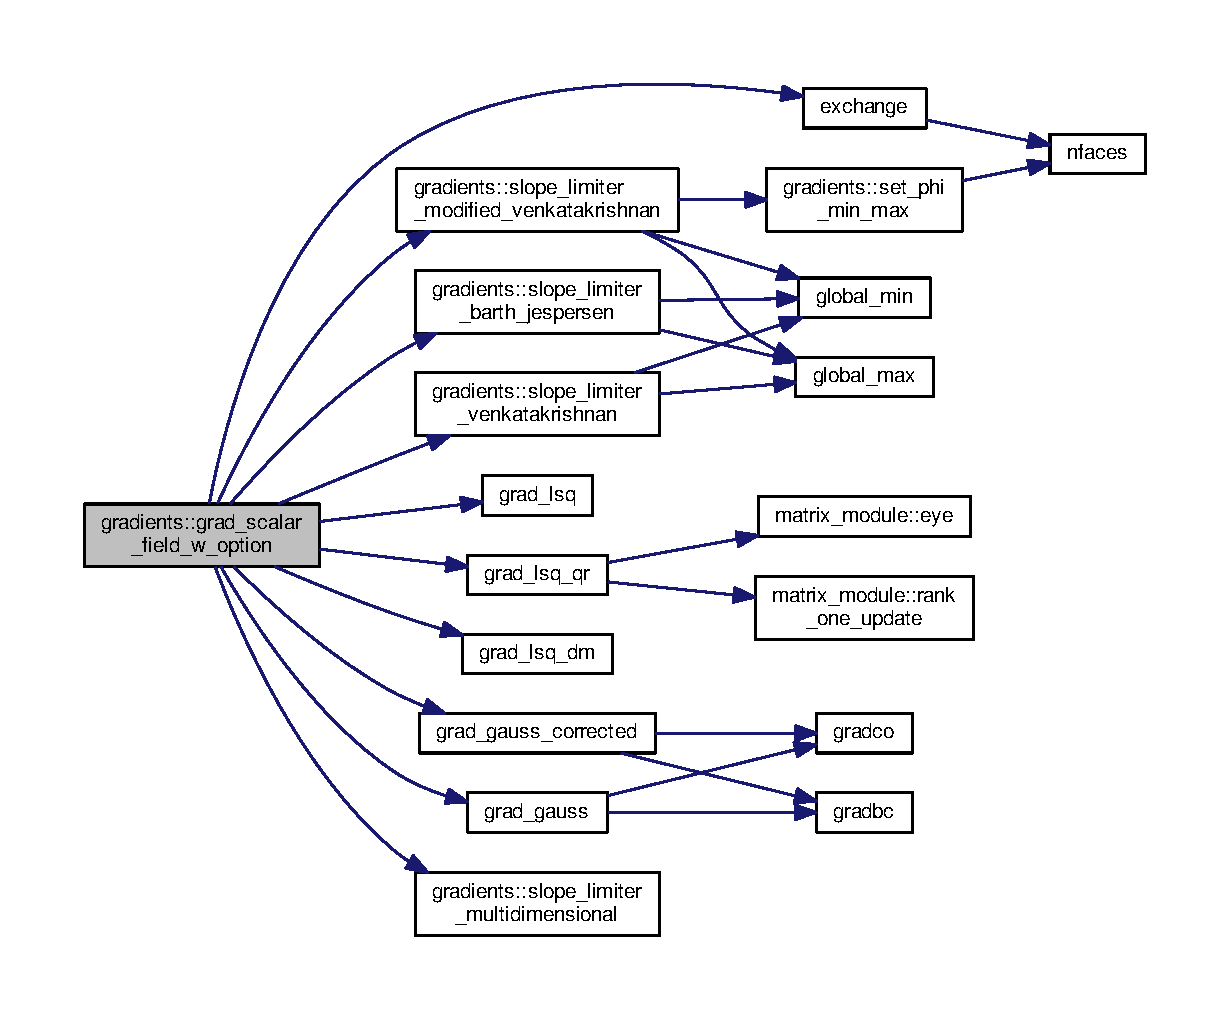
\includegraphics[width=350pt]{classgradients_a12593273fc9f5b56e9ddcad0f8945fa7_cgraph}
\end{center}
\end{figure}


\hypertarget{classgradients_a1cb60b38f23f9eb2ee50d537db912cfc}{\index{gradients@{gradients}!grad\-\_\-vector\-\_\-field@{grad\-\_\-vector\-\_\-field}}
\index{grad\-\_\-vector\-\_\-field@{grad\-\_\-vector\-\_\-field}!gradients@{gradients}}
\subsubsection[{grad\-\_\-vector\-\_\-field}]{\setlength{\rightskip}{0pt plus 5cm}subroutine gradients\-::grad\-\_\-vector\-\_\-field (
\begin{DoxyParamCaption}
\item[{real(dp), dimension(numtotal), intent(inout)}]{U, }
\item[{real(dp), dimension(numtotal), intent(inout)}]{V, }
\item[{real(dp), dimension(numtotal), intent(inout)}]{W, }
\item[{real(dp), dimension(3,numtotal), intent(inout)}]{d\-Udxi, }
\item[{real(dp), dimension(3,numtotal), intent(inout)}]{d\-Vdxi, }
\item[{real(dp), dimension(3,numtotal), intent(inout)}]{d\-Wdxi}
\end{DoxyParamCaption}
)\hspace{0.3cm}{\ttfamily [private]}}}\label{classgradients_a1cb60b38f23f9eb2ee50d537db912cfc}


Here is the call graph for this function\-:\nopagebreak
\begin{figure}[H]
\begin{center}
\leavevmode
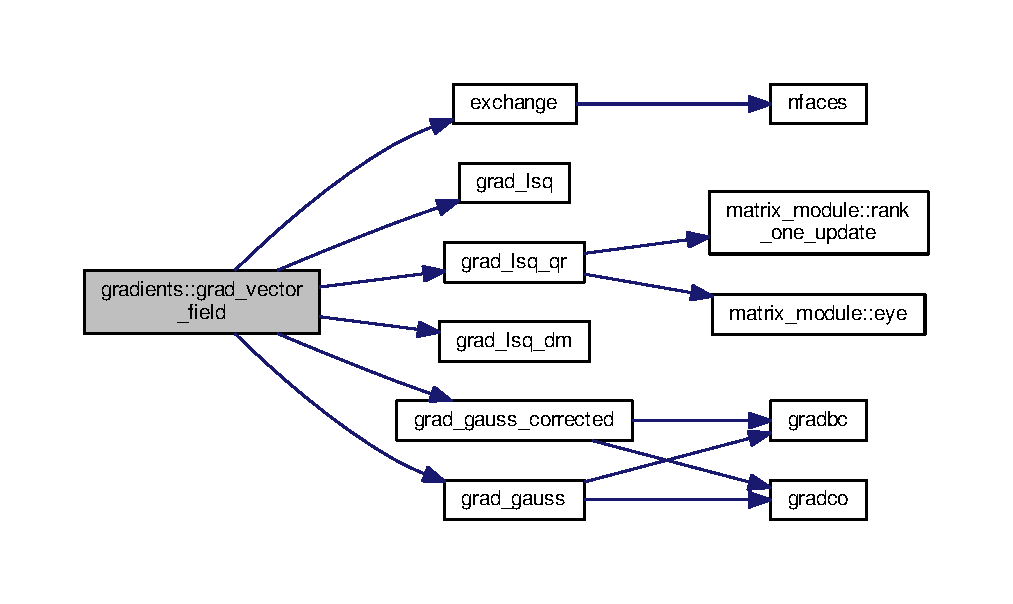
\includegraphics[width=350pt]{classgradients_a1cb60b38f23f9eb2ee50d537db912cfc_cgraph}
\end{center}
\end{figure}


\hypertarget{classgradients_abd2236c107f7c7c31c3f7fb638bb7b21}{\index{gradients@{gradients}!gradbc@{gradbc}}
\index{gradbc@{gradbc}!gradients@{gradients}}
\subsubsection[{gradbc}]{\setlength{\rightskip}{0pt plus 5cm}subroutine gradients\-::gradbc (
\begin{DoxyParamCaption}
\item[{real(dp), intent(in)}]{sx, }
\item[{real(dp), intent(in)}]{sy, }
\item[{real(dp), intent(in)}]{sz, }
\item[{real(dp), intent(in)}]{fi, }
\item[{real(dp), intent(inout)}]{dfx, }
\item[{real(dp), intent(inout)}]{dfy, }
\item[{real(dp), intent(inout)}]{dfz}
\end{DoxyParamCaption}
)}}\label{classgradients_abd2236c107f7c7c31c3f7fb638bb7b21}
\hypertarget{classgradients_a437864d9f0535f851ceb4272b256f4ea}{\index{gradients@{gradients}!gradco@{gradco}}
\index{gradco@{gradco}!gradients@{gradients}}
\subsubsection[{gradco}]{\setlength{\rightskip}{0pt plus 5cm}subroutine gradients\-::gradco (
\begin{DoxyParamCaption}
\item[{integer, intent(in)}]{ijp, }
\item[{integer, intent(in)}]{ijn, }
\item[{real(dp), intent(in)}]{xfc, }
\item[{real(dp), intent(in)}]{yfc, }
\item[{real(dp), intent(in)}]{zfc, }
\item[{real(dp), intent(in)}]{sx, }
\item[{real(dp), intent(in)}]{sy, }
\item[{real(dp), intent(in)}]{sz, }
\item[{real(dp), intent(in)}]{fif, }
\item[{real(dp), dimension(numtotal), intent(in)}]{fi, }
\item[{real(dp), dimension(numcells), intent(in)}]{dfxo, }
\item[{real(dp), dimension(numcells), intent(in)}]{dfyo, }
\item[{real(dp), dimension(numcells), intent(in)}]{dfzo, }
\item[{real(dp), dimension(numcells), intent(inout)}]{dfx, }
\item[{real(dp), dimension(numcells), intent(inout)}]{dfy, }
\item[{real(dp), dimension(numcells), intent(inout)}]{dfz}
\end{DoxyParamCaption}
)}}\label{classgradients_a437864d9f0535f851ceb4272b256f4ea}
\hypertarget{classgradients_a95333310c398e2b695c12e0d388000d9}{\index{gradients@{gradients}!gradcopar@{gradcopar}}
\index{gradcopar@{gradcopar}!gradients@{gradients}}
\subsubsection[{gradcopar}]{\setlength{\rightskip}{0pt plus 5cm}subroutine gradients\-::gradcopar (
\begin{DoxyParamCaption}
\item[{integer, intent(in)}]{ijp, }
\item[{integer, intent(in)}]{ijn, }
\item[{integer, intent(in)}]{ijnp, }
\item[{real(dp), intent(in)}]{xfc, }
\item[{real(dp), intent(in)}]{yfc, }
\item[{real(dp), intent(in)}]{zfc, }
\item[{real(dp), intent(in)}]{sx, }
\item[{real(dp), intent(in)}]{sy, }
\item[{real(dp), intent(in)}]{sz, }
\item[{real(dp), intent(in)}]{fif, }
\item[{real(dp), dimension(numtotal), intent(in)}]{fi, }
\item[{real(dp), dimension(numcells), intent(in)}]{dfxo, }
\item[{real(dp), dimension(numcells), intent(in)}]{dfyo, }
\item[{real(dp), dimension(numcells), intent(in)}]{dfzo, }
\item[{real(dp), dimension(numcells), intent(inout)}]{dfx, }
\item[{real(dp), dimension(numcells), intent(inout)}]{dfy, }
\item[{real(dp), dimension(numcells), intent(inout)}]{dfz}
\end{DoxyParamCaption}
)}}\label{classgradients_a95333310c398e2b695c12e0d388000d9}
\hypertarget{classgradients_af5ae74b1fab366ce3167820e0c6c5c3d}{\index{gradients@{gradients}!set\-\_\-phi\-\_\-min\-\_\-max@{set\-\_\-phi\-\_\-min\-\_\-max}}
\index{set\-\_\-phi\-\_\-min\-\_\-max@{set\-\_\-phi\-\_\-min\-\_\-max}!gradients@{gradients}}
\subsubsection[{set\-\_\-phi\-\_\-min\-\_\-max}]{\setlength{\rightskip}{0pt plus 5cm}subroutine gradients\-::set\-\_\-phi\-\_\-min\-\_\-max (
\begin{DoxyParamCaption}
\item[{real(dp), dimension(numtotal)}]{phi}
\end{DoxyParamCaption}
)\hspace{0.3cm}{\ttfamily [private]}}}\label{classgradients_af5ae74b1fab366ce3167820e0c6c5c3d}


Here is the call graph for this function\-:\nopagebreak
\begin{figure}[H]
\begin{center}
\leavevmode
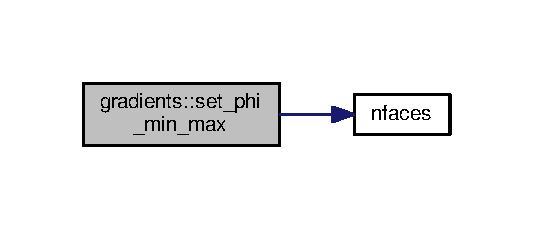
\includegraphics[width=256pt]{classgradients_af5ae74b1fab366ce3167820e0c6c5c3d_cgraph}
\end{center}
\end{figure}


\hypertarget{classgradients_ab7860442796eb435f5c34667b8c7c008}{\index{gradients@{gradients}!slope\-\_\-limiter\-\_\-barth\-\_\-jespersen@{slope\-\_\-limiter\-\_\-barth\-\_\-jespersen}}
\index{slope\-\_\-limiter\-\_\-barth\-\_\-jespersen@{slope\-\_\-limiter\-\_\-barth\-\_\-jespersen}!gradients@{gradients}}
\subsubsection[{slope\-\_\-limiter\-\_\-barth\-\_\-jespersen}]{\setlength{\rightskip}{0pt plus 5cm}subroutine gradients\-::slope\-\_\-limiter\-\_\-barth\-\_\-jespersen (
\begin{DoxyParamCaption}
\item[{real(dp), dimension(numtotal)}]{phi, }
\item[{real(dp), dimension(3,numtotal)}]{d\-Phidxi}
\end{DoxyParamCaption}
)}}\label{classgradients_ab7860442796eb435f5c34667b8c7c008}


Here is the call graph for this function\-:\nopagebreak
\begin{figure}[H]
\begin{center}
\leavevmode
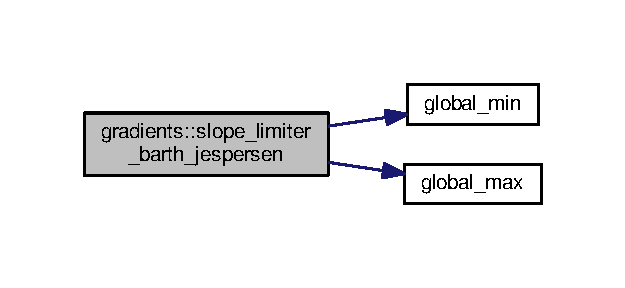
\includegraphics[width=300pt]{classgradients_ab7860442796eb435f5c34667b8c7c008_cgraph}
\end{center}
\end{figure}


\hypertarget{classgradients_af8d86227570d2a05536bc966c46f3fef}{\index{gradients@{gradients}!slope\-\_\-limiter\-\_\-modified\-\_\-venkatakrishnan@{slope\-\_\-limiter\-\_\-modified\-\_\-venkatakrishnan}}
\index{slope\-\_\-limiter\-\_\-modified\-\_\-venkatakrishnan@{slope\-\_\-limiter\-\_\-modified\-\_\-venkatakrishnan}!gradients@{gradients}}
\subsubsection[{slope\-\_\-limiter\-\_\-modified\-\_\-venkatakrishnan}]{\setlength{\rightskip}{0pt plus 5cm}subroutine gradients\-::slope\-\_\-limiter\-\_\-modified\-\_\-venkatakrishnan (
\begin{DoxyParamCaption}
\item[{real(dp), dimension(numtotal)}]{phi, }
\item[{real(dp), dimension(3,numtotal)}]{d\-Phidxi}
\end{DoxyParamCaption}
)}}\label{classgradients_af8d86227570d2a05536bc966c46f3fef}


Here is the call graph for this function\-:\nopagebreak
\begin{figure}[H]
\begin{center}
\leavevmode
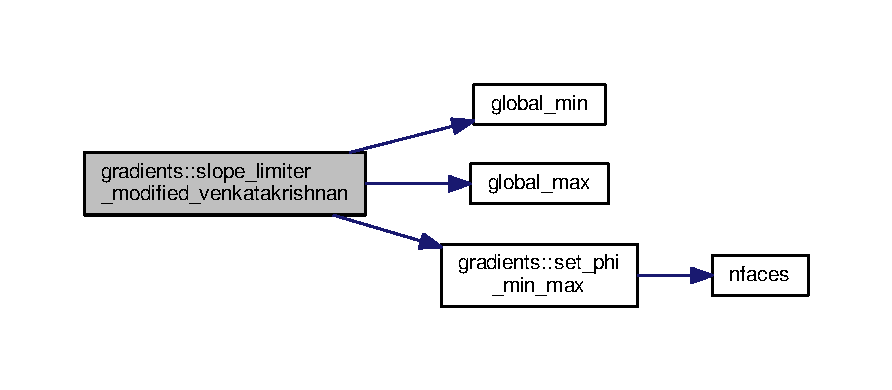
\includegraphics[width=350pt]{classgradients_af8d86227570d2a05536bc966c46f3fef_cgraph}
\end{center}
\end{figure}


\hypertarget{classgradients_a5392f6682ac037eae87dbe5f20d1205f}{\index{gradients@{gradients}!slope\-\_\-limiter\-\_\-multidimensional@{slope\-\_\-limiter\-\_\-multidimensional}}
\index{slope\-\_\-limiter\-\_\-multidimensional@{slope\-\_\-limiter\-\_\-multidimensional}!gradients@{gradients}}
\subsubsection[{slope\-\_\-limiter\-\_\-multidimensional}]{\setlength{\rightskip}{0pt plus 5cm}subroutine gradients\-::slope\-\_\-limiter\-\_\-multidimensional (
\begin{DoxyParamCaption}
\item[{real(dp), dimension(numtotal)}]{phi, }
\item[{real(dp), dimension(3,numcells)}]{d\-Phidxi}
\end{DoxyParamCaption}
)\hspace{0.3cm}{\ttfamily [private]}}}\label{classgradients_a5392f6682ac037eae87dbe5f20d1205f}
\hypertarget{classgradients_a19b76f98ae2657d4f6c3710bd2d8d0be}{\index{gradients@{gradients}!slope\-\_\-limiter\-\_\-venkatakrishnan@{slope\-\_\-limiter\-\_\-venkatakrishnan}}
\index{slope\-\_\-limiter\-\_\-venkatakrishnan@{slope\-\_\-limiter\-\_\-venkatakrishnan}!gradients@{gradients}}
\subsubsection[{slope\-\_\-limiter\-\_\-venkatakrishnan}]{\setlength{\rightskip}{0pt plus 5cm}subroutine gradients\-::slope\-\_\-limiter\-\_\-venkatakrishnan (
\begin{DoxyParamCaption}
\item[{real(dp), dimension(numtotal)}]{phi, }
\item[{real(dp), dimension(3,numtotal)}]{d\-Phidxi}
\end{DoxyParamCaption}
)\hspace{0.3cm}{\ttfamily [private]}}}\label{classgradients_a19b76f98ae2657d4f6c3710bd2d8d0be}


Here is the call graph for this function\-:\nopagebreak
\begin{figure}[H]
\begin{center}
\leavevmode
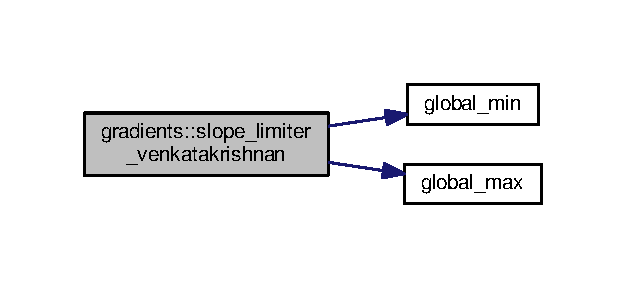
\includegraphics[width=300pt]{classgradients_a19b76f98ae2657d4f6c3710bd2d8d0be_cgraph}
\end{center}
\end{figure}


\hypertarget{classgradients_adcec95a6cfc9fbeb540b8a4a457bb2c6}{\index{gradients@{gradients}!sngrad\-\_\-scalar\-\_\-field@{sngrad\-\_\-scalar\-\_\-field}}
\index{sngrad\-\_\-scalar\-\_\-field@{sngrad\-\_\-scalar\-\_\-field}!gradients@{gradients}}
\subsubsection[{sngrad\-\_\-scalar\-\_\-field}]{\setlength{\rightskip}{0pt plus 5cm}subroutine gradients\-::sngrad\-\_\-scalar\-\_\-field (
\begin{DoxyParamCaption}
\item[{integer, intent(in)}]{ijp, }
\item[{integer, intent(in)}]{ijn, }
\item[{real(dp), intent(in)}]{xf, }
\item[{real(dp), intent(in)}]{yf, }
\item[{real(dp), intent(in)}]{zf, }
\item[{real(dp), intent(in)}]{arx, }
\item[{real(dp), intent(in)}]{ary, }
\item[{real(dp), intent(in)}]{arz, }
\item[{real(dp), intent(in)}]{lambda, }
\item[{real(dp), dimension(numtotal), intent(in)}]{Fi, }
\item[{real(dp), dimension(3,numtotal), intent(in)}]{d\-Fidxi, }
\item[{integer, intent(in)}]{nrelax, }
\item[{character(len=12)}]{approach, }
\item[{real(dp), intent(out)}]{dfixi, }
\item[{real(dp), intent(out)}]{dfiyi, }
\item[{real(dp), intent(out)}]{dfizi, }
\item[{real(dp), intent(out)}]{dfixii, }
\item[{real(dp), intent(out)}]{dfiyii, }
\item[{real(dp), intent(out)}]{dfizii}
\end{DoxyParamCaption}
)}}\label{classgradients_adcec95a6cfc9fbeb540b8a4a457bb2c6}
\hypertarget{classgradients_a85591b848f22ed6fefebedf8f90e9246}{\index{gradients@{gradients}!sngrad\-\_\-vector\-\_\-field@{sngrad\-\_\-vector\-\_\-field}}
\index{sngrad\-\_\-vector\-\_\-field@{sngrad\-\_\-vector\-\_\-field}!gradients@{gradients}}
\subsubsection[{sngrad\-\_\-vector\-\_\-field}]{\setlength{\rightskip}{0pt plus 5cm}subroutine gradients\-::sngrad\-\_\-vector\-\_\-field (
\begin{DoxyParamCaption}
\item[{integer, intent(in)}]{ijp, }
\item[{integer, intent(in)}]{ijn, }
\item[{real(dp), intent(in)}]{xf, }
\item[{real(dp), intent(in)}]{yf, }
\item[{real(dp), intent(in)}]{zf, }
\item[{real(dp), intent(in)}]{arx, }
\item[{real(dp), intent(in)}]{ary, }
\item[{real(dp), intent(in)}]{arz, }
\item[{real(dp), intent(in)}]{lambda, }
\item[{real(dp), dimension(numtotal), intent(in)}]{u, }
\item[{real(dp), dimension(numtotal), intent(in)}]{v, }
\item[{real(dp), dimension(numtotal), intent(in)}]{w, }
\item[{real(dp), dimension(3,numtotal), intent(in)}]{dudxi, }
\item[{real(dp), dimension(3,numtotal), intent(in)}]{dvdxi, }
\item[{real(dp), dimension(3,numtotal), intent(in)}]{dwdxi, }
\item[{integer, intent(in)}]{nrelax, }
\item[{character(len=12)}]{approach, }
\item[{real(dp), intent(out)}]{duxi, }
\item[{real(dp), intent(out)}]{duyi, }
\item[{real(dp), intent(out)}]{duzi, }
\item[{real(dp), intent(out)}]{dvxi, }
\item[{real(dp), intent(out)}]{dvyi, }
\item[{real(dp), intent(out)}]{dvzi, }
\item[{real(dp), intent(out)}]{dwxi, }
\item[{real(dp), intent(out)}]{dwyi, }
\item[{real(dp), intent(out)}]{dwzi, }
\item[{real(dp), intent(out)}]{duxii, }
\item[{real(dp), intent(out)}]{dvxii, }
\item[{real(dp), intent(out)}]{dwxii, }
\item[{real(dp), intent(out)}]{duyii, }
\item[{real(dp), intent(out)}]{dvyii, }
\item[{real(dp), intent(out)}]{dwyii, }
\item[{real(dp), intent(out)}]{duzii, }
\item[{real(dp), intent(out)}]{dvzii, }
\item[{real(dp), intent(out)}]{dwzii}
\end{DoxyParamCaption}
)\hspace{0.3cm}{\ttfamily [private]}}}\label{classgradients_a85591b848f22ed6fefebedf8f90e9246}


\subsection{Member Data Documentation}
\hypertarget{classgradients_a0417bd090ffd38c01cbcc0d76068dd82}{\index{gradients@{gradients}!dmat@{dmat}}
\index{dmat@{dmat}!gradients@{gradients}}
\subsubsection[{dmat}]{\setlength{\rightskip}{0pt plus 5cm}real(dp), dimension(\-:,\-:), allocatable, save gradients\-::dmat}}\label{classgradients_a0417bd090ffd38c01cbcc0d76068dd82}
\hypertarget{classgradients_a916054df6a0aaa257f536e0ef098b188}{\index{gradients@{gradients}!dmatqr@{dmatqr}}
\index{dmatqr@{dmatqr}!gradients@{gradients}}
\subsubsection[{dmatqr}]{\setlength{\rightskip}{0pt plus 5cm}real(dp), dimension(\-:,\-:,\-:), allocatable gradients\-::dmatqr}}\label{classgradients_a916054df6a0aaa257f536e0ef098b188}
\hypertarget{classgradients_ac41921915930ac80ed01373fd760ac51}{\index{gradients@{gradients}!gauss@{gauss}}
\index{gauss@{gauss}!gradients@{gradients}}
\subsubsection[{gauss}]{\setlength{\rightskip}{0pt plus 5cm}logical, public gradients\-::gauss}}\label{classgradients_ac41921915930ac80ed01373fd760ac51}
\hypertarget{classgradients_a47d37226aa24f4261a63b5cb1fa3d17c}{\index{gradients@{gradients}!limiter@{limiter}}
\index{limiter@{limiter}!gradients@{gradients}}
\subsubsection[{limiter}]{\setlength{\rightskip}{0pt plus 5cm}character(len=20), public gradients\-::limiter}}\label{classgradients_a47d37226aa24f4261a63b5cb1fa3d17c}
\hypertarget{classgradients_a4ef80ad8cc52782050167ed49c332c1e}{\index{gradients@{gradients}!lstsq@{lstsq}}
\index{lstsq@{lstsq}!gradients@{gradients}}
\subsubsection[{lstsq}]{\setlength{\rightskip}{0pt plus 5cm}logical, public gradients\-::lstsq}}\label{classgradients_a4ef80ad8cc52782050167ed49c332c1e}
\hypertarget{classgradients_a65547c6133cbc486266ac66604342516}{\index{gradients@{gradients}!lstsq\-\_\-dm@{lstsq\-\_\-dm}}
\index{lstsq\-\_\-dm@{lstsq\-\_\-dm}!gradients@{gradients}}
\subsubsection[{lstsq\-\_\-dm}]{\setlength{\rightskip}{0pt plus 5cm}logical, public gradients\-::lstsq\-\_\-dm}}\label{classgradients_a65547c6133cbc486266ac66604342516}
\hypertarget{classgradients_ae25a8c84c0815435812f94b82d7dafb7}{\index{gradients@{gradients}!lstsq\-\_\-qr@{lstsq\-\_\-qr}}
\index{lstsq\-\_\-qr@{lstsq\-\_\-qr}!gradients@{gradients}}
\subsubsection[{lstsq\-\_\-qr}]{\setlength{\rightskip}{0pt plus 5cm}logical, public gradients\-::lstsq\-\_\-qr}}\label{classgradients_ae25a8c84c0815435812f94b82d7dafb7}
\hypertarget{classgradients_ae02e791dcca067360cb4c1802dd6ef8d}{\index{gradients@{gradients}!sngrad\-\_\-corr@{sngrad\-\_\-corr}}
\index{sngrad\-\_\-corr@{sngrad\-\_\-corr}!gradients@{gradients}}
\subsubsection[{sngrad\-\_\-corr}]{\setlength{\rightskip}{0pt plus 5cm}character(len=12), public gradients\-::sngrad\-\_\-corr}}\label{classgradients_ae02e791dcca067360cb4c1802dd6ef8d}


The documentation for this module was generated from the following file\-:\begin{DoxyCompactItemize}
\item 
src-\/par/\hyperlink{gradients_8f90}{gradients.\-f90}\end{DoxyCompactItemize}

\hypertarget{classhcoef}{\section{hcoef Module Reference}
\label{classhcoef}\index{hcoef@{hcoef}}
}
\subsection*{Public Attributes}
\begin{DoxyCompactItemize}
\item 
real(dp), dimension(\-:), allocatable \hyperlink{classhcoef_a0fe90253d788ab22a12015d18132d8bf}{h}
\item 
real(dp), dimension(\-:), allocatable \hyperlink{classhcoef_aac65983f64ce20a3ddb35933d35cb78b}{hpr}
\item 
real(dp), dimension(\-:), allocatable \hyperlink{classhcoef_abff8e220ad240114fdb4775dcf026ca1}{ru}
\item 
real(dp), dimension(\-:), allocatable \hyperlink{classhcoef_a817f137e681d7382d4ac542179b85cb2}{rv}
\item 
real(dp), dimension(\-:), allocatable \hyperlink{classhcoef_a10cd6a89a20929137ddb8a7a9d29ba2d}{rw}
\end{DoxyCompactItemize}


\subsection{Member Data Documentation}
\hypertarget{classhcoef_a0fe90253d788ab22a12015d18132d8bf}{\index{hcoef@{hcoef}!h@{h}}
\index{h@{h}!hcoef@{hcoef}}
\subsubsection[{h}]{\setlength{\rightskip}{0pt plus 5cm}real(dp), dimension(\-:), allocatable hcoef\-::h}}\label{classhcoef_a0fe90253d788ab22a12015d18132d8bf}
\hypertarget{classhcoef_aac65983f64ce20a3ddb35933d35cb78b}{\index{hcoef@{hcoef}!hpr@{hpr}}
\index{hpr@{hpr}!hcoef@{hcoef}}
\subsubsection[{hpr}]{\setlength{\rightskip}{0pt plus 5cm}real(dp), dimension(\-:), allocatable hcoef\-::hpr}}\label{classhcoef_aac65983f64ce20a3ddb35933d35cb78b}
\hypertarget{classhcoef_abff8e220ad240114fdb4775dcf026ca1}{\index{hcoef@{hcoef}!ru@{ru}}
\index{ru@{ru}!hcoef@{hcoef}}
\subsubsection[{ru}]{\setlength{\rightskip}{0pt plus 5cm}real(dp), dimension(\-:), allocatable hcoef\-::ru}}\label{classhcoef_abff8e220ad240114fdb4775dcf026ca1}
\hypertarget{classhcoef_a817f137e681d7382d4ac542179b85cb2}{\index{hcoef@{hcoef}!rv@{rv}}
\index{rv@{rv}!hcoef@{hcoef}}
\subsubsection[{rv}]{\setlength{\rightskip}{0pt plus 5cm}real(dp), dimension(\-:), allocatable hcoef\-::rv}}\label{classhcoef_a817f137e681d7382d4ac542179b85cb2}
\hypertarget{classhcoef_a10cd6a89a20929137ddb8a7a9d29ba2d}{\index{hcoef@{hcoef}!rw@{rw}}
\index{rw@{rw}!hcoef@{hcoef}}
\subsubsection[{rw}]{\setlength{\rightskip}{0pt plus 5cm}real(dp), dimension(\-:), allocatable hcoef\-::rw}}\label{classhcoef_a10cd6a89a20929137ddb8a7a9d29ba2d}


The documentation for this module was generated from the following file\-:\begin{DoxyCompactItemize}
\item 
src-\/par/\hyperlink{modules__allocatable_8f90}{modules\-\_\-allocatable.\-f90}\end{DoxyCompactItemize}

\hypertarget{classinterpolation}{\section{interpolation Module Reference}
\label{classinterpolation}\index{interpolation@{interpolation}}
}
\subsection*{Public Member Functions}
\begin{DoxyCompactItemize}
\item 
real(dp) function \hyperlink{classinterpolation_a4906644e7abbc98fe9e87749dd7ca907}{face\-\_\-value} (\hyperlink{CourantNo_8h_accea320a458bb8759c7ece360e05ddf4}{ijp}, ijn, xf, yf, zf, lambda, u, d\-Udxi)
\item 
real(dp) function \hyperlink{classinterpolation_a2955420d11e2fbe30a99e4fefc374759}{face\-\_\-value\-\_\-cds} (\hyperlink{CourantNo_8h_accea320a458bb8759c7ece360e05ddf4}{ijp}, ijn, lambda, fi)
\item 
real(dp) function \hyperlink{classinterpolation_aebfa91890374b7e5e59f1342aa091a58}{face\-\_\-value\-\_\-cds\-\_\-corrected} (\hyperlink{CourantNo_8h_accea320a458bb8759c7ece360e05ddf4}{ijp}, ijn, xf, yf, zf, lambda, fi, dfidxi)
\item 
real(dp) function \hyperlink{classinterpolation_ab244a4491720b6c92b4f5e6e2539e06c}{face\-\_\-value\-\_\-central} (inp, inn, xf, yf, zf, fi, gradfi)
\item 
real(dp) function \hyperlink{classinterpolation_aad6795e9522c835edaf6484a063343cc}{face\-\_\-value\-\_\-2nd\-\_\-upwind} (inp, xf, yf, zf, fi, gradfi)
\item 
real(dp) function \hyperlink{classinterpolation_a69b9fafef9c399b908b8c8b6b7c7862d}{face\-\_\-value\-\_\-muscl} (inp, inn, xf, yf, zf, fi, gradfi)
\item 
real(dp) function \hyperlink{classinterpolation_af5ae37f4a0cb45e47998b454659a6eb9}{face\-\_\-value\-\_\-2nd\-\_\-upwind\-\_\-flux\-\_\-limiter} (\hyperlink{CourantNo_8h_accea320a458bb8759c7ece360e05ddf4}{ijp}, ijn, lambda, u, d\-Udxi)
\end{DoxyCompactItemize}


\subsection{Member Function/\-Subroutine Documentation}
\hypertarget{classinterpolation_a4906644e7abbc98fe9e87749dd7ca907}{\index{interpolation@{interpolation}!face\-\_\-value@{face\-\_\-value}}
\index{face\-\_\-value@{face\-\_\-value}!interpolation@{interpolation}}
\subsubsection[{face\-\_\-value}]{\setlength{\rightskip}{0pt plus 5cm}real(dp) function interpolation\-::face\-\_\-value (
\begin{DoxyParamCaption}
\item[{integer}]{ijp, }
\item[{integer}]{ijn, }
\item[{real(dp)}]{xf, }
\item[{real(dp)}]{yf, }
\item[{real(dp)}]{zf, }
\item[{real(dp)}]{lambda, }
\item[{real(dp), dimension(numtotal)}]{u, }
\item[{real(dp), dimension(3,numpcells)}]{d\-Udxi}
\end{DoxyParamCaption}
)}}\label{classinterpolation_a4906644e7abbc98fe9e87749dd7ca907}


Here is the call graph for this function\-:\nopagebreak
\begin{figure}[H]
\begin{center}
\leavevmode
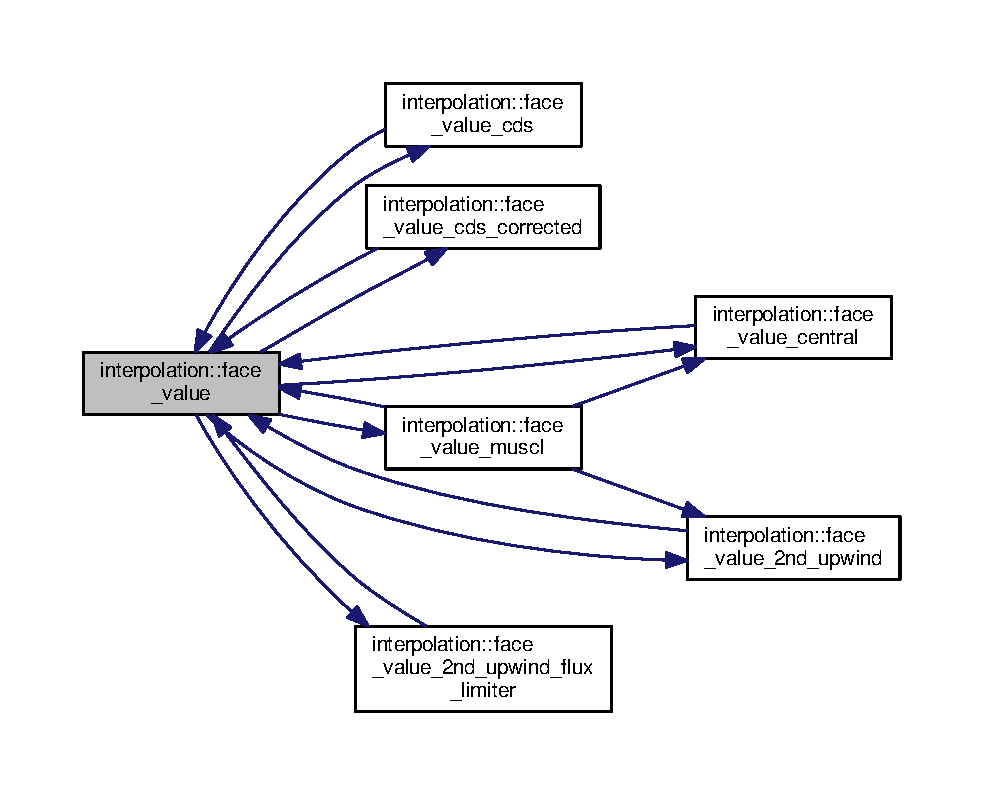
\includegraphics[width=350pt]{classinterpolation_a4906644e7abbc98fe9e87749dd7ca907_cgraph}
\end{center}
\end{figure}


\hypertarget{classinterpolation_aad6795e9522c835edaf6484a063343cc}{\index{interpolation@{interpolation}!face\-\_\-value\-\_\-2nd\-\_\-upwind@{face\-\_\-value\-\_\-2nd\-\_\-upwind}}
\index{face\-\_\-value\-\_\-2nd\-\_\-upwind@{face\-\_\-value\-\_\-2nd\-\_\-upwind}!interpolation@{interpolation}}
\subsubsection[{face\-\_\-value\-\_\-2nd\-\_\-upwind}]{\setlength{\rightskip}{0pt plus 5cm}real(dp) function interpolation\-::face\-\_\-value\-\_\-2nd\-\_\-upwind (
\begin{DoxyParamCaption}
\item[{integer}]{inp, }
\item[{real(dp)}]{xf, }
\item[{real(dp)}]{yf, }
\item[{real(dp)}]{zf, }
\item[{real(dp), dimension(numtotal)}]{fi, }
\item[{real(dp), dimension(3,numpcells)}]{gradfi}
\end{DoxyParamCaption}
)}}\label{classinterpolation_aad6795e9522c835edaf6484a063343cc}


Here is the call graph for this function\-:\nopagebreak
\begin{figure}[H]
\begin{center}
\leavevmode
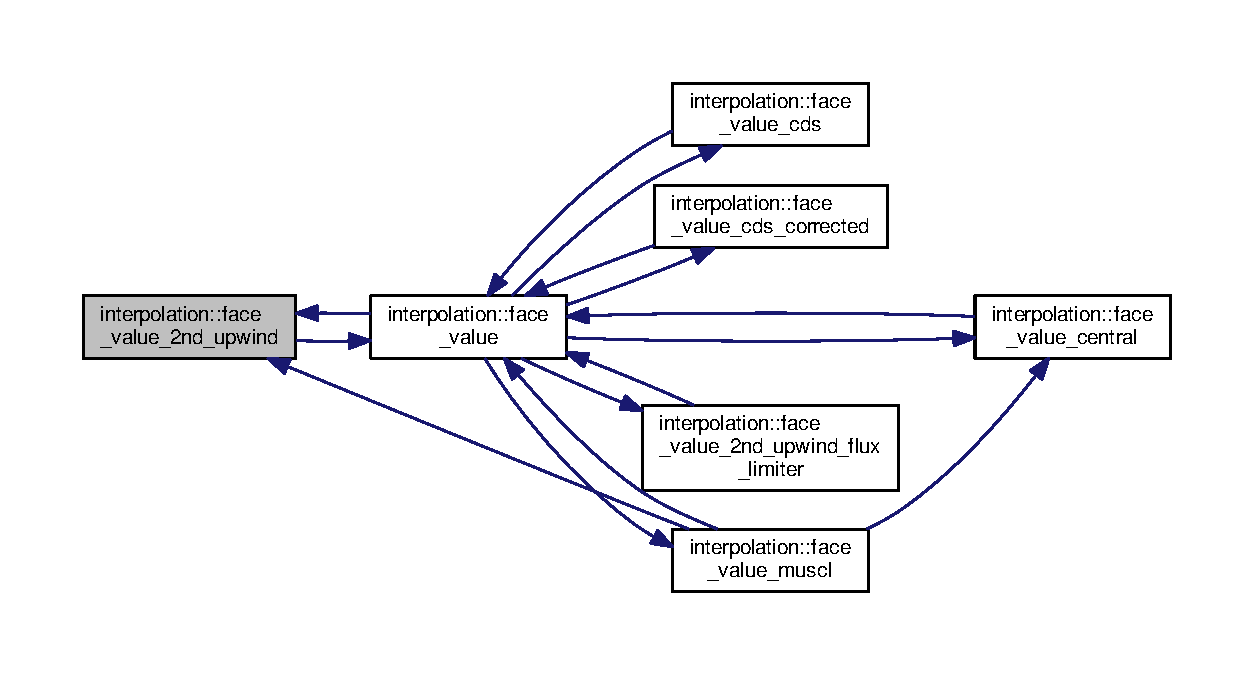
\includegraphics[width=350pt]{classinterpolation_aad6795e9522c835edaf6484a063343cc_cgraph}
\end{center}
\end{figure}


\hypertarget{classinterpolation_af5ae37f4a0cb45e47998b454659a6eb9}{\index{interpolation@{interpolation}!face\-\_\-value\-\_\-2nd\-\_\-upwind\-\_\-flux\-\_\-limiter@{face\-\_\-value\-\_\-2nd\-\_\-upwind\-\_\-flux\-\_\-limiter}}
\index{face\-\_\-value\-\_\-2nd\-\_\-upwind\-\_\-flux\-\_\-limiter@{face\-\_\-value\-\_\-2nd\-\_\-upwind\-\_\-flux\-\_\-limiter}!interpolation@{interpolation}}
\subsubsection[{face\-\_\-value\-\_\-2nd\-\_\-upwind\-\_\-flux\-\_\-limiter}]{\setlength{\rightskip}{0pt plus 5cm}real(dp) function interpolation\-::face\-\_\-value\-\_\-2nd\-\_\-upwind\-\_\-flux\-\_\-limiter (
\begin{DoxyParamCaption}
\item[{integer}]{ijp, }
\item[{integer}]{ijn, }
\item[{real(dp)}]{lambda, }
\item[{real(dp), dimension(numtotal)}]{u, }
\item[{real(dp), dimension(3,numpcells)}]{d\-Udxi}
\end{DoxyParamCaption}
)}}\label{classinterpolation_af5ae37f4a0cb45e47998b454659a6eb9}


Here is the call graph for this function\-:\nopagebreak
\begin{figure}[H]
\begin{center}
\leavevmode
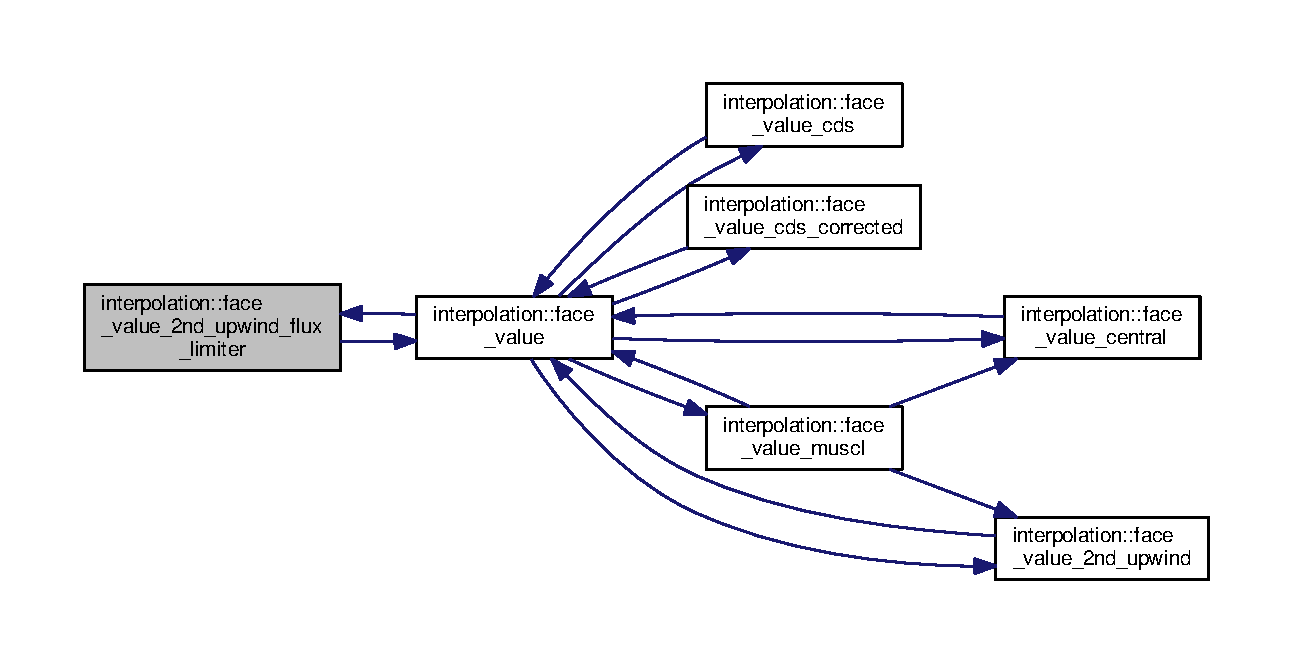
\includegraphics[width=350pt]{classinterpolation_af5ae37f4a0cb45e47998b454659a6eb9_cgraph}
\end{center}
\end{figure}


\hypertarget{classinterpolation_a2955420d11e2fbe30a99e4fefc374759}{\index{interpolation@{interpolation}!face\-\_\-value\-\_\-cds@{face\-\_\-value\-\_\-cds}}
\index{face\-\_\-value\-\_\-cds@{face\-\_\-value\-\_\-cds}!interpolation@{interpolation}}
\subsubsection[{face\-\_\-value\-\_\-cds}]{\setlength{\rightskip}{0pt plus 5cm}real(dp) function interpolation\-::face\-\_\-value\-\_\-cds (
\begin{DoxyParamCaption}
\item[{integer}]{ijp, }
\item[{integer}]{ijn, }
\item[{real(dp)}]{lambda, }
\item[{real(dp), dimension(numtotal)}]{fi}
\end{DoxyParamCaption}
)}}\label{classinterpolation_a2955420d11e2fbe30a99e4fefc374759}


Here is the call graph for this function\-:\nopagebreak
\begin{figure}[H]
\begin{center}
\leavevmode
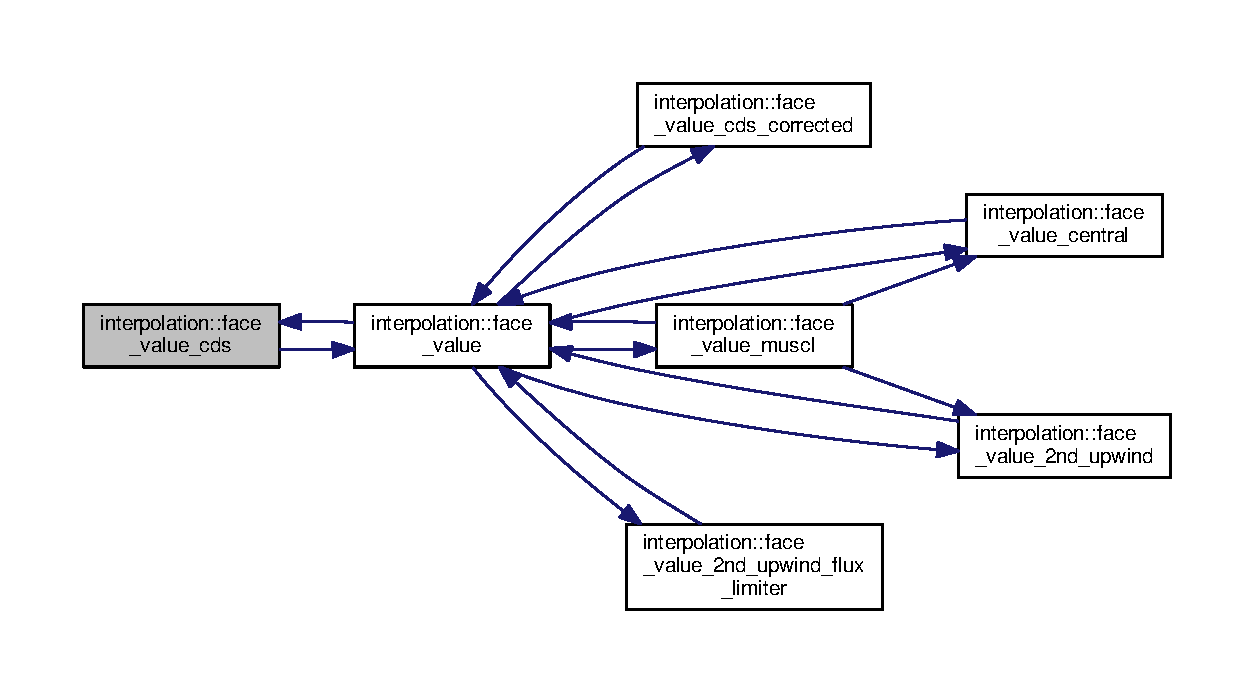
\includegraphics[width=350pt]{classinterpolation_a2955420d11e2fbe30a99e4fefc374759_cgraph}
\end{center}
\end{figure}


\hypertarget{classinterpolation_aebfa91890374b7e5e59f1342aa091a58}{\index{interpolation@{interpolation}!face\-\_\-value\-\_\-cds\-\_\-corrected@{face\-\_\-value\-\_\-cds\-\_\-corrected}}
\index{face\-\_\-value\-\_\-cds\-\_\-corrected@{face\-\_\-value\-\_\-cds\-\_\-corrected}!interpolation@{interpolation}}
\subsubsection[{face\-\_\-value\-\_\-cds\-\_\-corrected}]{\setlength{\rightskip}{0pt plus 5cm}real(dp) function interpolation\-::face\-\_\-value\-\_\-cds\-\_\-corrected (
\begin{DoxyParamCaption}
\item[{integer}]{ijp, }
\item[{integer}]{ijn, }
\item[{real(dp)}]{xf, }
\item[{real(dp)}]{yf, }
\item[{real(dp)}]{zf, }
\item[{real(dp)}]{lambda, }
\item[{real(dp), dimension(numtotal)}]{fi, }
\item[{real(dp), dimension(3,numpcells)}]{dfidxi}
\end{DoxyParamCaption}
)}}\label{classinterpolation_aebfa91890374b7e5e59f1342aa091a58}


Here is the call graph for this function\-:\nopagebreak
\begin{figure}[H]
\begin{center}
\leavevmode
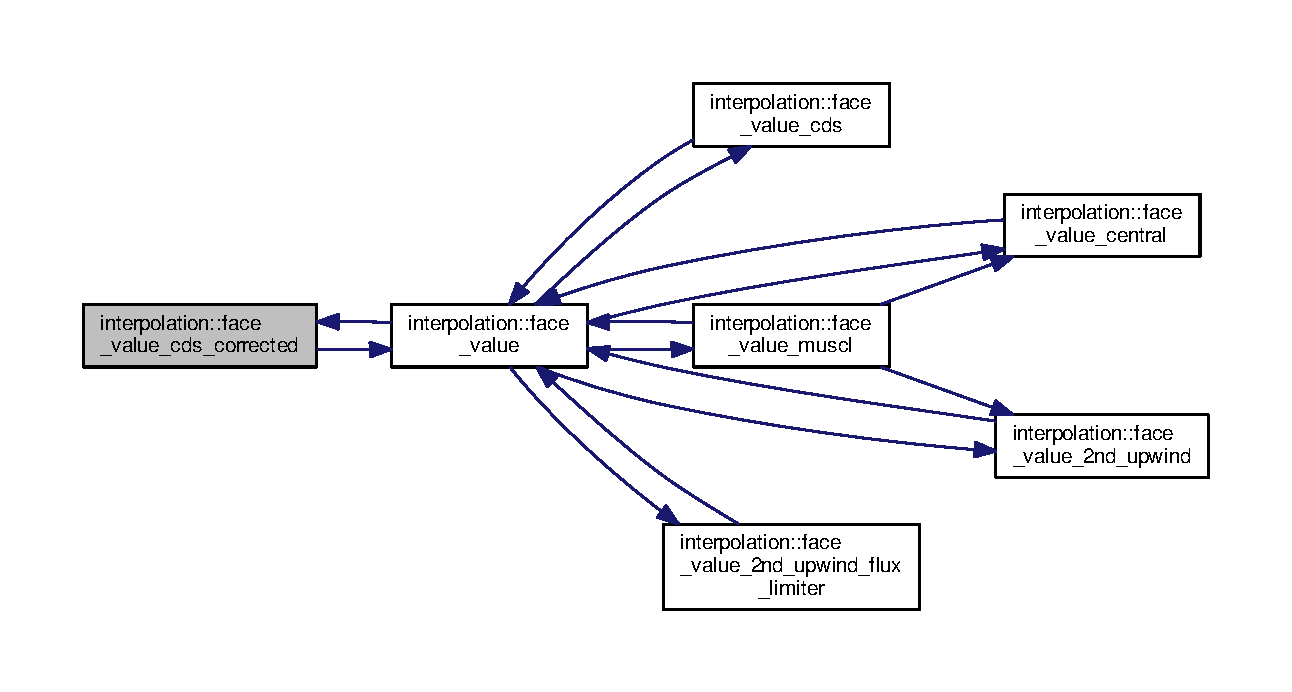
\includegraphics[width=350pt]{classinterpolation_aebfa91890374b7e5e59f1342aa091a58_cgraph}
\end{center}
\end{figure}


\hypertarget{classinterpolation_ab244a4491720b6c92b4f5e6e2539e06c}{\index{interpolation@{interpolation}!face\-\_\-value\-\_\-central@{face\-\_\-value\-\_\-central}}
\index{face\-\_\-value\-\_\-central@{face\-\_\-value\-\_\-central}!interpolation@{interpolation}}
\subsubsection[{face\-\_\-value\-\_\-central}]{\setlength{\rightskip}{0pt plus 5cm}real(dp) function interpolation\-::face\-\_\-value\-\_\-central (
\begin{DoxyParamCaption}
\item[{integer}]{inp, }
\item[{integer}]{inn, }
\item[{real(dp)}]{xf, }
\item[{real(dp)}]{yf, }
\item[{real(dp)}]{zf, }
\item[{real(dp), dimension(numtotal)}]{fi, }
\item[{real(dp), dimension(3,numpcells)}]{gradfi}
\end{DoxyParamCaption}
)}}\label{classinterpolation_ab244a4491720b6c92b4f5e6e2539e06c}


Here is the call graph for this function\-:\nopagebreak
\begin{figure}[H]
\begin{center}
\leavevmode
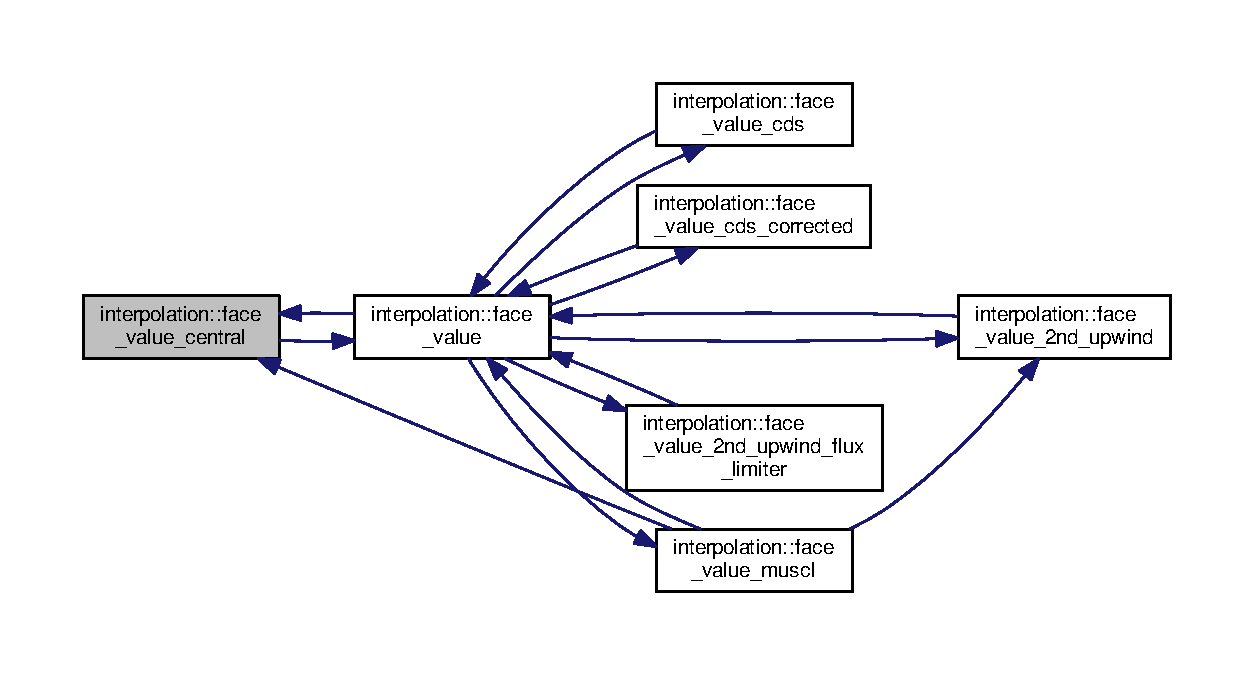
\includegraphics[width=350pt]{classinterpolation_ab244a4491720b6c92b4f5e6e2539e06c_cgraph}
\end{center}
\end{figure}


\hypertarget{classinterpolation_a69b9fafef9c399b908b8c8b6b7c7862d}{\index{interpolation@{interpolation}!face\-\_\-value\-\_\-muscl@{face\-\_\-value\-\_\-muscl}}
\index{face\-\_\-value\-\_\-muscl@{face\-\_\-value\-\_\-muscl}!interpolation@{interpolation}}
\subsubsection[{face\-\_\-value\-\_\-muscl}]{\setlength{\rightskip}{0pt plus 5cm}real(dp) function interpolation\-::face\-\_\-value\-\_\-muscl (
\begin{DoxyParamCaption}
\item[{integer}]{inp, }
\item[{integer}]{inn, }
\item[{real(dp)}]{xf, }
\item[{real(dp)}]{yf, }
\item[{real(dp)}]{zf, }
\item[{real(dp), dimension(numtotal)}]{fi, }
\item[{real(dp), dimension(3,numpcells)}]{gradfi}
\end{DoxyParamCaption}
)}}\label{classinterpolation_a69b9fafef9c399b908b8c8b6b7c7862d}


Here is the call graph for this function\-:\nopagebreak
\begin{figure}[H]
\begin{center}
\leavevmode
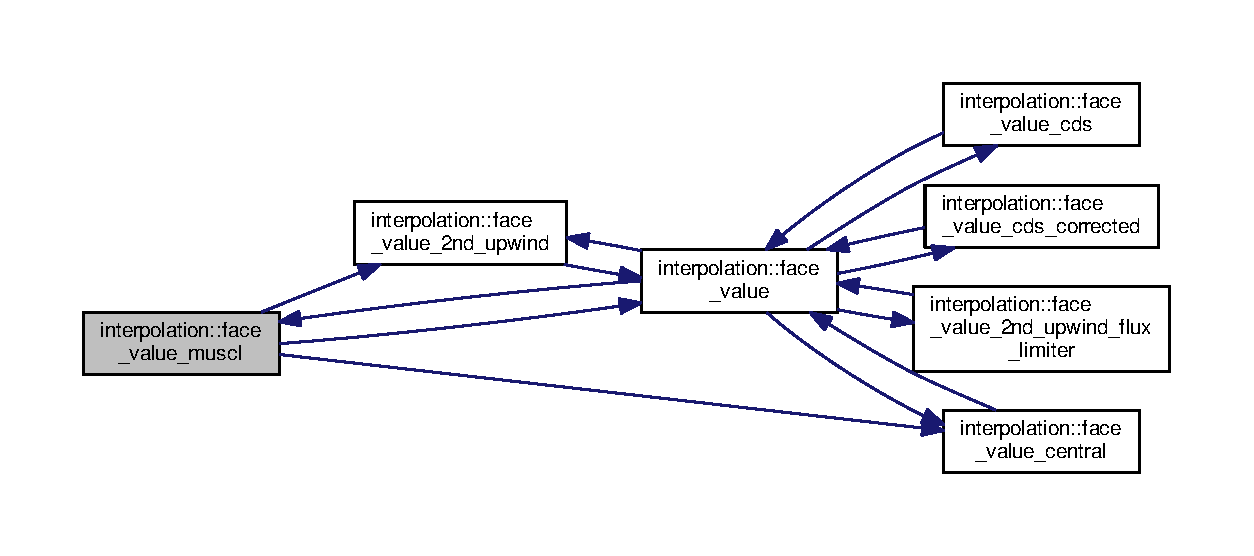
\includegraphics[width=350pt]{classinterpolation_a69b9fafef9c399b908b8c8b6b7c7862d_cgraph}
\end{center}
\end{figure}




The documentation for this module was generated from the following file\-:\begin{DoxyCompactItemize}
\item 
src-\/par/\hyperlink{interpolation_8f90}{interpolation.\-f90}\end{DoxyCompactItemize}

\hypertarget{classk__epsilon__rng}{\section{k\-\_\-epsilon\-\_\-rng Module Reference}
\label{classk__epsilon__rng}\index{k\-\_\-epsilon\-\_\-rng@{k\-\_\-epsilon\-\_\-rng}}
}
\subsection*{Public Member Functions}
\begin{DoxyCompactItemize}
\item 
subroutine, public \hyperlink{classk__epsilon__rng_aead60a1e254021f3eccd9fd8a7b74352}{correct\-\_\-turbulence\-\_\-k\-\_\-epsilon\-\_\-rng} ()
\item 
subroutine, public \hyperlink{classk__epsilon__rng_a26639f5f7047e9c797b92d7383543509}{correct\-\_\-turbulence\-\_\-inlet\-\_\-k\-\_\-epsilon\-\_\-rng} ()
\item 
subroutine \hyperlink{classk__epsilon__rng_a9b6328ba57554ef905a83eaa444b8d83}{modify\-\_\-mu\-\_\-eff} ()
\item 
subroutine \hyperlink{classk__epsilon__rng_ac9112e6bf146afd6c79028a23415676c}{modify\-\_\-mu\-\_\-eff\-\_\-inlet} ()
\end{DoxyCompactItemize}
\subsection*{Public Attributes}
\begin{DoxyCompactItemize}
\item 
real(dp), parameter \hyperlink{classk__epsilon__rng_a6b241c19c45ed08f9aa1f0a7e03b53d7}{cmu} = 0.\-0845\-\_\-dp
\item 
real(dp), parameter \hyperlink{classk__epsilon__rng_ad50599dfea881408b5cf48539f9ad517}{c1} = 1.\-42\-\_\-dp
\item 
real(dp), parameter \hyperlink{classk__epsilon__rng_a6a8f83178b54a12ab8bb88a8f87e4742}{c2} = 1.\-68\-\_\-dp
\item 
real(dp), parameter \hyperlink{classk__epsilon__rng_a60edd75f1fe3c0814506d06a17b7236a}{c3} = 1.\-44\-\_\-dp
\item 
real(dp), parameter \hyperlink{classk__epsilon__rng_a5acd8d27794527d80376d8dc66a15c80}{sigma\-\_\-k} = 0.\-7194\-\_\-dp
\item 
real(dp), parameter \hyperlink{classk__epsilon__rng_ad605a3725a59c2b4c42212222e9b8f0e}{sigma\-\_\-epsilon} = 0.\-7194\-\_\-dp
\item 
real(dp), parameter \hyperlink{classk__epsilon__rng_ad5f3f150214e5954d1b25097db147625}{cmu25} = sqrt(sqrt(\hyperlink{classk__epsilon__rng_a6b241c19c45ed08f9aa1f0a7e03b53d7}{cmu}))
\item 
real(dp), parameter \hyperlink{classk__epsilon__rng_aa8cce766b4ed7f38a8e55945cee9c659}{cmu75} = \hyperlink{classk__epsilon__rng_ad5f3f150214e5954d1b25097db147625}{cmu25}$\ast$$\ast$3
\end{DoxyCompactItemize}
\subsection*{Private Member Functions}
\begin{DoxyCompactItemize}
\item 
subroutine \hyperlink{classk__epsilon__rng_aa259d766694cc52d057ecf778fe2d5ea}{calcsc} (Fi, d\-Fidxi, ifi)
\end{DoxyCompactItemize}


\subsection{Member Function/\-Subroutine Documentation}
\hypertarget{classk__epsilon__rng_aa259d766694cc52d057ecf778fe2d5ea}{\index{k\-\_\-epsilon\-\_\-rng@{k\-\_\-epsilon\-\_\-rng}!calcsc@{calcsc}}
\index{calcsc@{calcsc}!k_epsilon_rng@{k\-\_\-epsilon\-\_\-rng}}
\subsubsection[{calcsc}]{\setlength{\rightskip}{0pt plus 5cm}subroutine k\-\_\-epsilon\-\_\-rng\-::calcsc (
\begin{DoxyParamCaption}
\item[{real(dp), dimension(numtotal)}]{Fi, }
\item[{real(dp), dimension(3,numcells)}]{d\-Fidxi, }
\item[{integer, intent(in)}]{ifi}
\end{DoxyParamCaption}
)\hspace{0.3cm}{\ttfamily [private]}}}\label{classk__epsilon__rng_aa259d766694cc52d057ecf778fe2d5ea}


Here is the call graph for this function\-:\nopagebreak
\begin{figure}[H]
\begin{center}
\leavevmode
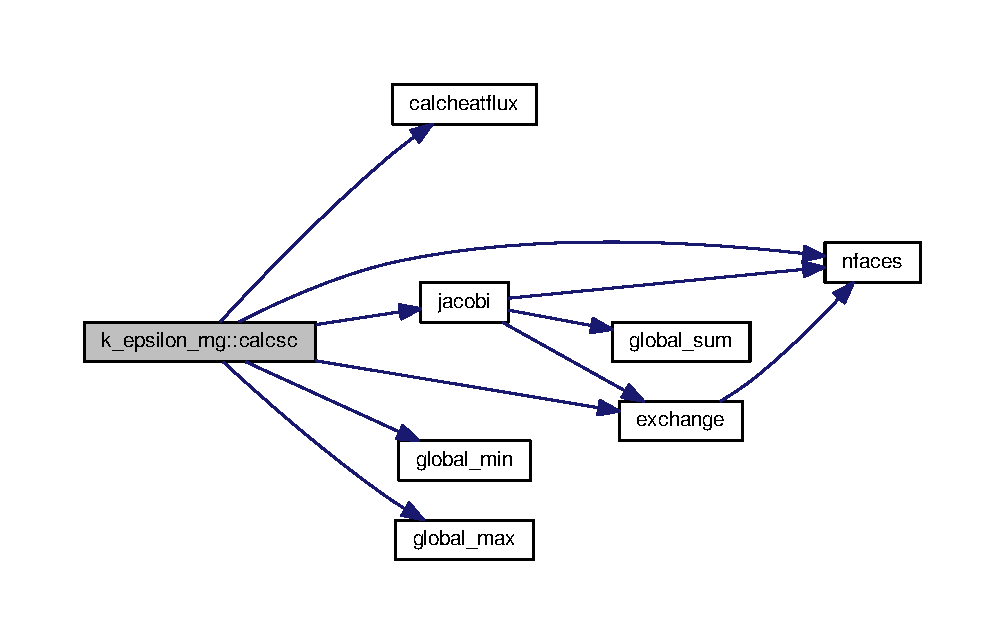
\includegraphics[width=350pt]{classk__epsilon__rng_aa259d766694cc52d057ecf778fe2d5ea_cgraph}
\end{center}
\end{figure}


\hypertarget{classk__epsilon__rng_a26639f5f7047e9c797b92d7383543509}{\index{k\-\_\-epsilon\-\_\-rng@{k\-\_\-epsilon\-\_\-rng}!correct\-\_\-turbulence\-\_\-inlet\-\_\-k\-\_\-epsilon\-\_\-rng@{correct\-\_\-turbulence\-\_\-inlet\-\_\-k\-\_\-epsilon\-\_\-rng}}
\index{correct\-\_\-turbulence\-\_\-inlet\-\_\-k\-\_\-epsilon\-\_\-rng@{correct\-\_\-turbulence\-\_\-inlet\-\_\-k\-\_\-epsilon\-\_\-rng}!k_epsilon_rng@{k\-\_\-epsilon\-\_\-rng}}
\subsubsection[{correct\-\_\-turbulence\-\_\-inlet\-\_\-k\-\_\-epsilon\-\_\-rng}]{\setlength{\rightskip}{0pt plus 5cm}subroutine, public k\-\_\-epsilon\-\_\-rng\-::correct\-\_\-turbulence\-\_\-inlet\-\_\-k\-\_\-epsilon\-\_\-rng (
\begin{DoxyParamCaption}
{}
\end{DoxyParamCaption}
)}}\label{classk__epsilon__rng_a26639f5f7047e9c797b92d7383543509}


Here is the call graph for this function\-:\nopagebreak
\begin{figure}[H]
\begin{center}
\leavevmode
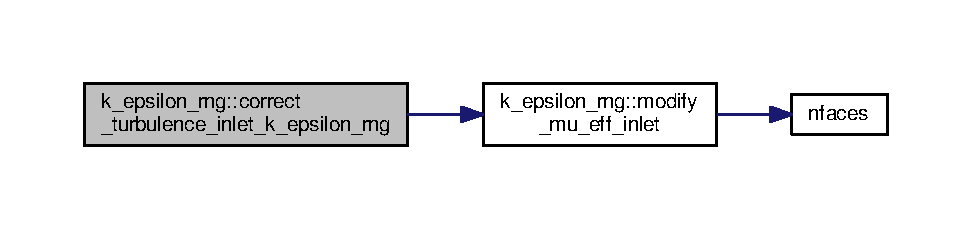
\includegraphics[width=350pt]{classk__epsilon__rng_a26639f5f7047e9c797b92d7383543509_cgraph}
\end{center}
\end{figure}


\hypertarget{classk__epsilon__rng_aead60a1e254021f3eccd9fd8a7b74352}{\index{k\-\_\-epsilon\-\_\-rng@{k\-\_\-epsilon\-\_\-rng}!correct\-\_\-turbulence\-\_\-k\-\_\-epsilon\-\_\-rng@{correct\-\_\-turbulence\-\_\-k\-\_\-epsilon\-\_\-rng}}
\index{correct\-\_\-turbulence\-\_\-k\-\_\-epsilon\-\_\-rng@{correct\-\_\-turbulence\-\_\-k\-\_\-epsilon\-\_\-rng}!k_epsilon_rng@{k\-\_\-epsilon\-\_\-rng}}
\subsubsection[{correct\-\_\-turbulence\-\_\-k\-\_\-epsilon\-\_\-rng}]{\setlength{\rightskip}{0pt plus 5cm}subroutine, public k\-\_\-epsilon\-\_\-rng\-::correct\-\_\-turbulence\-\_\-k\-\_\-epsilon\-\_\-rng (
\begin{DoxyParamCaption}
{}
\end{DoxyParamCaption}
)}}\label{classk__epsilon__rng_aead60a1e254021f3eccd9fd8a7b74352}


Here is the call graph for this function\-:\nopagebreak
\begin{figure}[H]
\begin{center}
\leavevmode
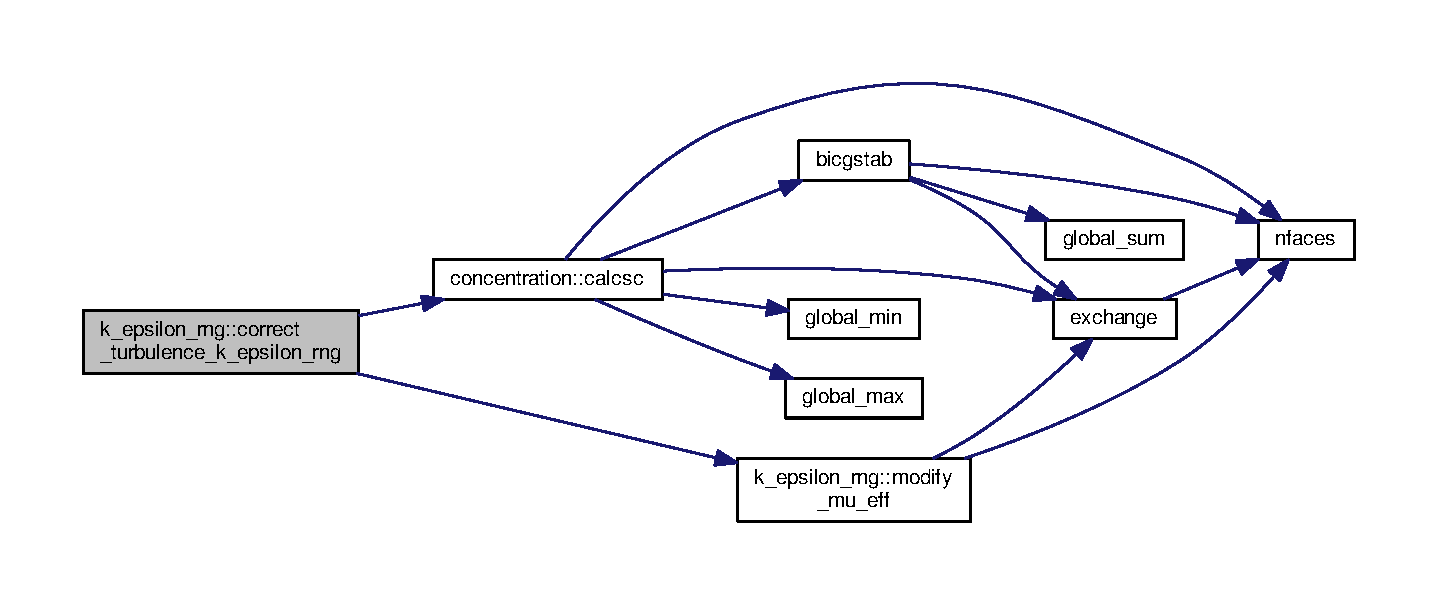
\includegraphics[width=350pt]{classk__epsilon__rng_aead60a1e254021f3eccd9fd8a7b74352_cgraph}
\end{center}
\end{figure}


\hypertarget{classk__epsilon__rng_a9b6328ba57554ef905a83eaa444b8d83}{\index{k\-\_\-epsilon\-\_\-rng@{k\-\_\-epsilon\-\_\-rng}!modify\-\_\-mu\-\_\-eff@{modify\-\_\-mu\-\_\-eff}}
\index{modify\-\_\-mu\-\_\-eff@{modify\-\_\-mu\-\_\-eff}!k_epsilon_rng@{k\-\_\-epsilon\-\_\-rng}}
\subsubsection[{modify\-\_\-mu\-\_\-eff}]{\setlength{\rightskip}{0pt plus 5cm}subroutine k\-\_\-epsilon\-\_\-rng\-::modify\-\_\-mu\-\_\-eff (
\begin{DoxyParamCaption}
{}
\end{DoxyParamCaption}
)}}\label{classk__epsilon__rng_a9b6328ba57554ef905a83eaa444b8d83}


Here is the call graph for this function\-:\nopagebreak
\begin{figure}[H]
\begin{center}
\leavevmode
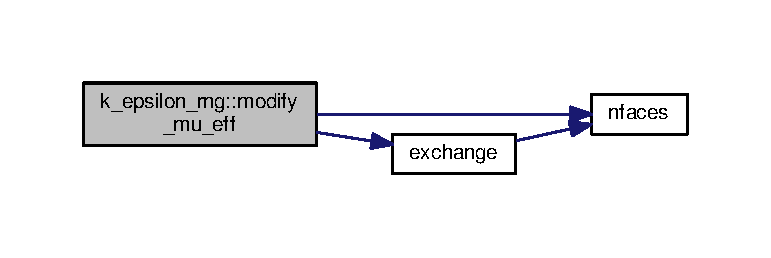
\includegraphics[width=350pt]{classk__epsilon__rng_a9b6328ba57554ef905a83eaa444b8d83_cgraph}
\end{center}
\end{figure}


\hypertarget{classk__epsilon__rng_ac9112e6bf146afd6c79028a23415676c}{\index{k\-\_\-epsilon\-\_\-rng@{k\-\_\-epsilon\-\_\-rng}!modify\-\_\-mu\-\_\-eff\-\_\-inlet@{modify\-\_\-mu\-\_\-eff\-\_\-inlet}}
\index{modify\-\_\-mu\-\_\-eff\-\_\-inlet@{modify\-\_\-mu\-\_\-eff\-\_\-inlet}!k_epsilon_rng@{k\-\_\-epsilon\-\_\-rng}}
\subsubsection[{modify\-\_\-mu\-\_\-eff\-\_\-inlet}]{\setlength{\rightskip}{0pt plus 5cm}subroutine k\-\_\-epsilon\-\_\-rng\-::modify\-\_\-mu\-\_\-eff\-\_\-inlet (
\begin{DoxyParamCaption}
{}
\end{DoxyParamCaption}
)}}\label{classk__epsilon__rng_ac9112e6bf146afd6c79028a23415676c}


Here is the call graph for this function\-:\nopagebreak
\begin{figure}[H]
\begin{center}
\leavevmode
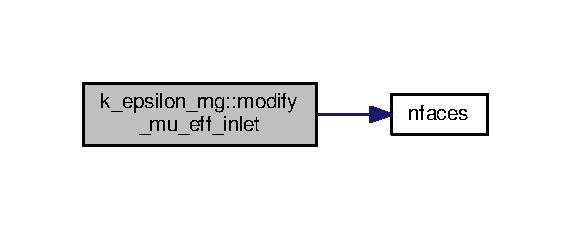
\includegraphics[width=274pt]{classk__epsilon__rng_ac9112e6bf146afd6c79028a23415676c_cgraph}
\end{center}
\end{figure}




\subsection{Member Data Documentation}
\hypertarget{classk__epsilon__rng_ad50599dfea881408b5cf48539f9ad517}{\index{k\-\_\-epsilon\-\_\-rng@{k\-\_\-epsilon\-\_\-rng}!c1@{c1}}
\index{c1@{c1}!k_epsilon_rng@{k\-\_\-epsilon\-\_\-rng}}
\subsubsection[{c1}]{\setlength{\rightskip}{0pt plus 5cm}real(dp), parameter k\-\_\-epsilon\-\_\-rng\-::c1 = 1.\-42\-\_\-dp}}\label{classk__epsilon__rng_ad50599dfea881408b5cf48539f9ad517}
\hypertarget{classk__epsilon__rng_a6a8f83178b54a12ab8bb88a8f87e4742}{\index{k\-\_\-epsilon\-\_\-rng@{k\-\_\-epsilon\-\_\-rng}!c2@{c2}}
\index{c2@{c2}!k_epsilon_rng@{k\-\_\-epsilon\-\_\-rng}}
\subsubsection[{c2}]{\setlength{\rightskip}{0pt plus 5cm}real(dp), parameter k\-\_\-epsilon\-\_\-rng\-::c2 = 1.\-68\-\_\-dp}}\label{classk__epsilon__rng_a6a8f83178b54a12ab8bb88a8f87e4742}
\hypertarget{classk__epsilon__rng_a60edd75f1fe3c0814506d06a17b7236a}{\index{k\-\_\-epsilon\-\_\-rng@{k\-\_\-epsilon\-\_\-rng}!c3@{c3}}
\index{c3@{c3}!k_epsilon_rng@{k\-\_\-epsilon\-\_\-rng}}
\subsubsection[{c3}]{\setlength{\rightskip}{0pt plus 5cm}real(dp), parameter k\-\_\-epsilon\-\_\-rng\-::c3 = 1.\-44\-\_\-dp}}\label{classk__epsilon__rng_a60edd75f1fe3c0814506d06a17b7236a}
\hypertarget{classk__epsilon__rng_a6b241c19c45ed08f9aa1f0a7e03b53d7}{\index{k\-\_\-epsilon\-\_\-rng@{k\-\_\-epsilon\-\_\-rng}!cmu@{cmu}}
\index{cmu@{cmu}!k_epsilon_rng@{k\-\_\-epsilon\-\_\-rng}}
\subsubsection[{cmu}]{\setlength{\rightskip}{0pt plus 5cm}real(dp), parameter k\-\_\-epsilon\-\_\-rng\-::cmu = 0.\-0845\-\_\-dp}}\label{classk__epsilon__rng_a6b241c19c45ed08f9aa1f0a7e03b53d7}
\hypertarget{classk__epsilon__rng_ad5f3f150214e5954d1b25097db147625}{\index{k\-\_\-epsilon\-\_\-rng@{k\-\_\-epsilon\-\_\-rng}!cmu25@{cmu25}}
\index{cmu25@{cmu25}!k_epsilon_rng@{k\-\_\-epsilon\-\_\-rng}}
\subsubsection[{cmu25}]{\setlength{\rightskip}{0pt plus 5cm}real(dp), parameter k\-\_\-epsilon\-\_\-rng\-::cmu25 = sqrt(sqrt({\bf cmu}))}}\label{classk__epsilon__rng_ad5f3f150214e5954d1b25097db147625}
\hypertarget{classk__epsilon__rng_aa8cce766b4ed7f38a8e55945cee9c659}{\index{k\-\_\-epsilon\-\_\-rng@{k\-\_\-epsilon\-\_\-rng}!cmu75@{cmu75}}
\index{cmu75@{cmu75}!k_epsilon_rng@{k\-\_\-epsilon\-\_\-rng}}
\subsubsection[{cmu75}]{\setlength{\rightskip}{0pt plus 5cm}real(dp), parameter k\-\_\-epsilon\-\_\-rng\-::cmu75 = {\bf cmu25}$\ast$$\ast$3}}\label{classk__epsilon__rng_aa8cce766b4ed7f38a8e55945cee9c659}
\hypertarget{classk__epsilon__rng_ad605a3725a59c2b4c42212222e9b8f0e}{\index{k\-\_\-epsilon\-\_\-rng@{k\-\_\-epsilon\-\_\-rng}!sigma\-\_\-epsilon@{sigma\-\_\-epsilon}}
\index{sigma\-\_\-epsilon@{sigma\-\_\-epsilon}!k_epsilon_rng@{k\-\_\-epsilon\-\_\-rng}}
\subsubsection[{sigma\-\_\-epsilon}]{\setlength{\rightskip}{0pt plus 5cm}real(dp), parameter k\-\_\-epsilon\-\_\-rng\-::sigma\-\_\-epsilon = 0.\-7194\-\_\-dp}}\label{classk__epsilon__rng_ad605a3725a59c2b4c42212222e9b8f0e}
\hypertarget{classk__epsilon__rng_a5acd8d27794527d80376d8dc66a15c80}{\index{k\-\_\-epsilon\-\_\-rng@{k\-\_\-epsilon\-\_\-rng}!sigma\-\_\-k@{sigma\-\_\-k}}
\index{sigma\-\_\-k@{sigma\-\_\-k}!k_epsilon_rng@{k\-\_\-epsilon\-\_\-rng}}
\subsubsection[{sigma\-\_\-k}]{\setlength{\rightskip}{0pt plus 5cm}real(dp), parameter k\-\_\-epsilon\-\_\-rng\-::sigma\-\_\-k = 0.\-7194\-\_\-dp}}\label{classk__epsilon__rng_a5acd8d27794527d80376d8dc66a15c80}


The documentation for this module was generated from the following file\-:\begin{DoxyCompactItemize}
\item 
src-\/par/\hyperlink{k__epsilon__rng_8f90}{k\-\_\-epsilon\-\_\-rng.\-f90}\end{DoxyCompactItemize}

\hypertarget{classk__epsilon__std}{\section{k\-\_\-epsilon\-\_\-std Module Reference}
\label{classk__epsilon__std}\index{k\-\_\-epsilon\-\_\-std@{k\-\_\-epsilon\-\_\-std}}
}
\subsection*{Public Member Functions}
\begin{DoxyCompactItemize}
\item 
subroutine, public \hyperlink{classk__epsilon__std_aba071419bae84ce7a551ad2786481333}{correct\-\_\-turbulence\-\_\-k\-\_\-epsilon\-\_\-std} ()
\item 
subroutine, public \hyperlink{classk__epsilon__std_a1f9fe4f360a65f9d3f13c90cc30870b0}{correct\-\_\-turbulence\-\_\-inlet\-\_\-k\-\_\-epsilon\-\_\-std} ()
\item 
subroutine \hyperlink{classk__epsilon__std_a0a532283b523bd70158bf79b67d8d70e}{modify\-\_\-mu\-\_\-eff} ()
\item 
subroutine \hyperlink{classk__epsilon__std_a67a34b9f9d0599206952688d26e0d903}{modify\-\_\-mu\-\_\-eff\-\_\-inlet} ()
\end{DoxyCompactItemize}
\subsection*{Public Attributes}
\begin{DoxyCompactItemize}
\item 
real(dp), parameter \hyperlink{classk__epsilon__std_ab8b45782adecbcc30ebf7b73d34a5ebd}{cmu} = 0.\-09\-\_\-dp
\item 
real(dp), parameter \hyperlink{classk__epsilon__std_a93ff6c4e5f083bc36a60209c171035f8}{c1} = 1.\-44\-\_\-dp
\item 
real(dp), parameter \hyperlink{classk__epsilon__std_a42ad7b9456f3e4d745d15cbfa7dd05c9}{c2} = 1.\-92\-\_\-dp
\item 
real(dp), parameter \hyperlink{classk__epsilon__std_a95e68b7b052df6838c3c516dd66cf0c5}{c3} = 1.\-44\-\_\-dp
\item 
real(dp), parameter \hyperlink{classk__epsilon__std_a6fa05e7c5d25ef3f137a8fbf3523f86e}{sigma\-\_\-k} = 1.\-0\-\_\-dp
\item 
real(dp), parameter \hyperlink{classk__epsilon__std_a915f88270b38c6960c564a1e62b30a4b}{sigma\-\_\-epsilon} = 1.\-3\-\_\-dp
\item 
real(dp), parameter \hyperlink{classk__epsilon__std_a5560ee6203c001281958b7335769e6e4}{cmu25} = sqrt(sqrt(\hyperlink{classk__epsilon__std_ab8b45782adecbcc30ebf7b73d34a5ebd}{cmu}))
\item 
real(dp), parameter \hyperlink{classk__epsilon__std_a385af61636cbfd6cd867898d54c297f1}{cmu75} = \hyperlink{classk__epsilon__std_a5560ee6203c001281958b7335769e6e4}{cmu25}$\ast$$\ast$3
\end{DoxyCompactItemize}
\subsection*{Private Member Functions}
\begin{DoxyCompactItemize}
\item 
subroutine \hyperlink{classk__epsilon__std_a154b083087bab8a4573406234b03da78}{calcsc} (Fi, d\-Fidxi, ifi)
\end{DoxyCompactItemize}


\subsection{Member Function/\-Subroutine Documentation}
\hypertarget{classk__epsilon__std_a154b083087bab8a4573406234b03da78}{\index{k\-\_\-epsilon\-\_\-std@{k\-\_\-epsilon\-\_\-std}!calcsc@{calcsc}}
\index{calcsc@{calcsc}!k_epsilon_std@{k\-\_\-epsilon\-\_\-std}}
\subsubsection[{calcsc}]{\setlength{\rightskip}{0pt plus 5cm}subroutine k\-\_\-epsilon\-\_\-std\-::calcsc (
\begin{DoxyParamCaption}
\item[{real(dp), dimension(numtotal)}]{Fi, }
\item[{real(dp), dimension(3,numcells)}]{d\-Fidxi, }
\item[{integer, intent(in)}]{ifi}
\end{DoxyParamCaption}
)\hspace{0.3cm}{\ttfamily [private]}}}\label{classk__epsilon__std_a154b083087bab8a4573406234b03da78}


Here is the call graph for this function\-:\nopagebreak
\begin{figure}[H]
\begin{center}
\leavevmode
\includegraphics[width=350pt]{classk__epsilon__std_a154b083087bab8a4573406234b03da78_cgraph}
\end{center}
\end{figure}


\hypertarget{classk__epsilon__std_a1f9fe4f360a65f9d3f13c90cc30870b0}{\index{k\-\_\-epsilon\-\_\-std@{k\-\_\-epsilon\-\_\-std}!correct\-\_\-turbulence\-\_\-inlet\-\_\-k\-\_\-epsilon\-\_\-std@{correct\-\_\-turbulence\-\_\-inlet\-\_\-k\-\_\-epsilon\-\_\-std}}
\index{correct\-\_\-turbulence\-\_\-inlet\-\_\-k\-\_\-epsilon\-\_\-std@{correct\-\_\-turbulence\-\_\-inlet\-\_\-k\-\_\-epsilon\-\_\-std}!k_epsilon_std@{k\-\_\-epsilon\-\_\-std}}
\subsubsection[{correct\-\_\-turbulence\-\_\-inlet\-\_\-k\-\_\-epsilon\-\_\-std}]{\setlength{\rightskip}{0pt plus 5cm}subroutine, public k\-\_\-epsilon\-\_\-std\-::correct\-\_\-turbulence\-\_\-inlet\-\_\-k\-\_\-epsilon\-\_\-std (
\begin{DoxyParamCaption}
{}
\end{DoxyParamCaption}
)}}\label{classk__epsilon__std_a1f9fe4f360a65f9d3f13c90cc30870b0}


Here is the call graph for this function\-:\nopagebreak
\begin{figure}[H]
\begin{center}
\leavevmode
\includegraphics[width=350pt]{classk__epsilon__std_a1f9fe4f360a65f9d3f13c90cc30870b0_cgraph}
\end{center}
\end{figure}


\hypertarget{classk__epsilon__std_aba071419bae84ce7a551ad2786481333}{\index{k\-\_\-epsilon\-\_\-std@{k\-\_\-epsilon\-\_\-std}!correct\-\_\-turbulence\-\_\-k\-\_\-epsilon\-\_\-std@{correct\-\_\-turbulence\-\_\-k\-\_\-epsilon\-\_\-std}}
\index{correct\-\_\-turbulence\-\_\-k\-\_\-epsilon\-\_\-std@{correct\-\_\-turbulence\-\_\-k\-\_\-epsilon\-\_\-std}!k_epsilon_std@{k\-\_\-epsilon\-\_\-std}}
\subsubsection[{correct\-\_\-turbulence\-\_\-k\-\_\-epsilon\-\_\-std}]{\setlength{\rightskip}{0pt plus 5cm}subroutine, public k\-\_\-epsilon\-\_\-std\-::correct\-\_\-turbulence\-\_\-k\-\_\-epsilon\-\_\-std (
\begin{DoxyParamCaption}
{}
\end{DoxyParamCaption}
)}}\label{classk__epsilon__std_aba071419bae84ce7a551ad2786481333}


Here is the call graph for this function\-:\nopagebreak
\begin{figure}[H]
\begin{center}
\leavevmode
\includegraphics[width=350pt]{classk__epsilon__std_aba071419bae84ce7a551ad2786481333_cgraph}
\end{center}
\end{figure}


\hypertarget{classk__epsilon__std_a0a532283b523bd70158bf79b67d8d70e}{\index{k\-\_\-epsilon\-\_\-std@{k\-\_\-epsilon\-\_\-std}!modify\-\_\-mu\-\_\-eff@{modify\-\_\-mu\-\_\-eff}}
\index{modify\-\_\-mu\-\_\-eff@{modify\-\_\-mu\-\_\-eff}!k_epsilon_std@{k\-\_\-epsilon\-\_\-std}}
\subsubsection[{modify\-\_\-mu\-\_\-eff}]{\setlength{\rightskip}{0pt plus 5cm}subroutine k\-\_\-epsilon\-\_\-std\-::modify\-\_\-mu\-\_\-eff (
\begin{DoxyParamCaption}
{}
\end{DoxyParamCaption}
)}}\label{classk__epsilon__std_a0a532283b523bd70158bf79b67d8d70e}


Here is the call graph for this function\-:\nopagebreak
\begin{figure}[H]
\begin{center}
\leavevmode
\includegraphics[width=350pt]{classk__epsilon__std_a0a532283b523bd70158bf79b67d8d70e_cgraph}
\end{center}
\end{figure}


\hypertarget{classk__epsilon__std_a67a34b9f9d0599206952688d26e0d903}{\index{k\-\_\-epsilon\-\_\-std@{k\-\_\-epsilon\-\_\-std}!modify\-\_\-mu\-\_\-eff\-\_\-inlet@{modify\-\_\-mu\-\_\-eff\-\_\-inlet}}
\index{modify\-\_\-mu\-\_\-eff\-\_\-inlet@{modify\-\_\-mu\-\_\-eff\-\_\-inlet}!k_epsilon_std@{k\-\_\-epsilon\-\_\-std}}
\subsubsection[{modify\-\_\-mu\-\_\-eff\-\_\-inlet}]{\setlength{\rightskip}{0pt plus 5cm}subroutine k\-\_\-epsilon\-\_\-std\-::modify\-\_\-mu\-\_\-eff\-\_\-inlet (
\begin{DoxyParamCaption}
{}
\end{DoxyParamCaption}
)}}\label{classk__epsilon__std_a67a34b9f9d0599206952688d26e0d903}


Here is the call graph for this function\-:\nopagebreak
\begin{figure}[H]
\begin{center}
\leavevmode
\includegraphics[width=274pt]{classk__epsilon__std_a67a34b9f9d0599206952688d26e0d903_cgraph}
\end{center}
\end{figure}




\subsection{Member Data Documentation}
\hypertarget{classk__epsilon__std_a93ff6c4e5f083bc36a60209c171035f8}{\index{k\-\_\-epsilon\-\_\-std@{k\-\_\-epsilon\-\_\-std}!c1@{c1}}
\index{c1@{c1}!k_epsilon_std@{k\-\_\-epsilon\-\_\-std}}
\subsubsection[{c1}]{\setlength{\rightskip}{0pt plus 5cm}real(dp), parameter k\-\_\-epsilon\-\_\-std\-::c1 = 1.\-44\-\_\-dp}}\label{classk__epsilon__std_a93ff6c4e5f083bc36a60209c171035f8}
\hypertarget{classk__epsilon__std_a42ad7b9456f3e4d745d15cbfa7dd05c9}{\index{k\-\_\-epsilon\-\_\-std@{k\-\_\-epsilon\-\_\-std}!c2@{c2}}
\index{c2@{c2}!k_epsilon_std@{k\-\_\-epsilon\-\_\-std}}
\subsubsection[{c2}]{\setlength{\rightskip}{0pt plus 5cm}real(dp), parameter k\-\_\-epsilon\-\_\-std\-::c2 = 1.\-92\-\_\-dp}}\label{classk__epsilon__std_a42ad7b9456f3e4d745d15cbfa7dd05c9}
\hypertarget{classk__epsilon__std_a95e68b7b052df6838c3c516dd66cf0c5}{\index{k\-\_\-epsilon\-\_\-std@{k\-\_\-epsilon\-\_\-std}!c3@{c3}}
\index{c3@{c3}!k_epsilon_std@{k\-\_\-epsilon\-\_\-std}}
\subsubsection[{c3}]{\setlength{\rightskip}{0pt plus 5cm}real(dp), parameter k\-\_\-epsilon\-\_\-std\-::c3 = 1.\-44\-\_\-dp}}\label{classk__epsilon__std_a95e68b7b052df6838c3c516dd66cf0c5}
\hypertarget{classk__epsilon__std_ab8b45782adecbcc30ebf7b73d34a5ebd}{\index{k\-\_\-epsilon\-\_\-std@{k\-\_\-epsilon\-\_\-std}!cmu@{cmu}}
\index{cmu@{cmu}!k_epsilon_std@{k\-\_\-epsilon\-\_\-std}}
\subsubsection[{cmu}]{\setlength{\rightskip}{0pt plus 5cm}real(dp), parameter k\-\_\-epsilon\-\_\-std\-::cmu = 0.\-09\-\_\-dp}}\label{classk__epsilon__std_ab8b45782adecbcc30ebf7b73d34a5ebd}
\hypertarget{classk__epsilon__std_a5560ee6203c001281958b7335769e6e4}{\index{k\-\_\-epsilon\-\_\-std@{k\-\_\-epsilon\-\_\-std}!cmu25@{cmu25}}
\index{cmu25@{cmu25}!k_epsilon_std@{k\-\_\-epsilon\-\_\-std}}
\subsubsection[{cmu25}]{\setlength{\rightskip}{0pt plus 5cm}real(dp), parameter k\-\_\-epsilon\-\_\-std\-::cmu25 = sqrt(sqrt({\bf cmu}))}}\label{classk__epsilon__std_a5560ee6203c001281958b7335769e6e4}
\hypertarget{classk__epsilon__std_a385af61636cbfd6cd867898d54c297f1}{\index{k\-\_\-epsilon\-\_\-std@{k\-\_\-epsilon\-\_\-std}!cmu75@{cmu75}}
\index{cmu75@{cmu75}!k_epsilon_std@{k\-\_\-epsilon\-\_\-std}}
\subsubsection[{cmu75}]{\setlength{\rightskip}{0pt plus 5cm}real(dp), parameter k\-\_\-epsilon\-\_\-std\-::cmu75 = {\bf cmu25}$\ast$$\ast$3}}\label{classk__epsilon__std_a385af61636cbfd6cd867898d54c297f1}
\hypertarget{classk__epsilon__std_a915f88270b38c6960c564a1e62b30a4b}{\index{k\-\_\-epsilon\-\_\-std@{k\-\_\-epsilon\-\_\-std}!sigma\-\_\-epsilon@{sigma\-\_\-epsilon}}
\index{sigma\-\_\-epsilon@{sigma\-\_\-epsilon}!k_epsilon_std@{k\-\_\-epsilon\-\_\-std}}
\subsubsection[{sigma\-\_\-epsilon}]{\setlength{\rightskip}{0pt plus 5cm}real(dp), parameter k\-\_\-epsilon\-\_\-std\-::sigma\-\_\-epsilon = 1.\-3\-\_\-dp}}\label{classk__epsilon__std_a915f88270b38c6960c564a1e62b30a4b}
\hypertarget{classk__epsilon__std_a6fa05e7c5d25ef3f137a8fbf3523f86e}{\index{k\-\_\-epsilon\-\_\-std@{k\-\_\-epsilon\-\_\-std}!sigma\-\_\-k@{sigma\-\_\-k}}
\index{sigma\-\_\-k@{sigma\-\_\-k}!k_epsilon_std@{k\-\_\-epsilon\-\_\-std}}
\subsubsection[{sigma\-\_\-k}]{\setlength{\rightskip}{0pt plus 5cm}real(dp), parameter k\-\_\-epsilon\-\_\-std\-::sigma\-\_\-k = 1.\-0\-\_\-dp}}\label{classk__epsilon__std_a6fa05e7c5d25ef3f137a8fbf3523f86e}


The documentation for this module was generated from the following file\-:\begin{DoxyCompactItemize}
\item 
src-\/par/\hyperlink{k__epsilon__std_8f90}{k\-\_\-epsilon\-\_\-std.\-f90}\end{DoxyCompactItemize}

\hypertarget{classk__epsilon__zeta__f}{\section{k\-\_\-epsilon\-\_\-zeta\-\_\-f Module Reference}
\label{classk__epsilon__zeta__f}\index{k\-\_\-epsilon\-\_\-zeta\-\_\-f@{k\-\_\-epsilon\-\_\-zeta\-\_\-f}}
}
\subsection*{Public Member Functions}
\begin{DoxyCompactItemize}
\item 
subroutine, public \hyperlink{classk__epsilon__zeta__f_a96d9ff45439b59d5b8335e39aad4d47d}{correct\-\_\-turbulence\-\_\-k\-\_\-epsilon\-\_\-zeta\-\_\-f} ()
\item 
subroutine, public \hyperlink{classk__epsilon__zeta__f_a7e80d54ab71f25e4596d0ca6a46ee4ba}{correct\-\_\-turbulence\-\_\-inlet\-\_\-k\-\_\-epsilon\-\_\-zeta\-\_\-f} ()
\item 
subroutine \hyperlink{classk__epsilon__zeta__f_aee004b7784046d5d09ef6090646cd0de}{modify\-\_\-mu\-\_\-eff} ()
\item 
subroutine \hyperlink{classk__epsilon__zeta__f_a2c14f0a38ce6658faca9884c37c791b4}{modify\-\_\-mu\-\_\-eff\-\_\-inlet} ()
\end{DoxyCompactItemize}
\subsection*{Public Attributes}
\begin{DoxyCompactItemize}
\item 
real(dp), parameter \hyperlink{classk__epsilon__zeta__f_a5d567a6368bca5b0841051cd221355d4}{cmu} = 0.\-22\-\_\-dp
\item 
real(dp), parameter \hyperlink{classk__epsilon__zeta__f_a45bedddf115b58d59169d1da64d873eb}{c1} = 1.\-4\-\_\-dp
\item 
real(dp) \hyperlink{classk__epsilon__zeta__f_a424dc1473dde87fac65394097c5a045f}{ceps1}
\item 
real(dp), parameter \hyperlink{classk__epsilon__zeta__f_a9ebcc0eb612e02b54b59ef242fb0c21c}{ceps2} = 1.\-9\-\_\-dp
\item 
real(dp), parameter \hyperlink{classk__epsilon__zeta__f_af3e889088961660782f1a7e4406edee3}{c2p} = 0.\-65\-\_\-dp
\item 
real(dp), parameter \hyperlink{classk__epsilon__zeta__f_a54620cbb76d5c8b3260c4f8037170965}{ct} = 6.\-0\-\_\-dp
\item 
real(dp), parameter \hyperlink{classk__epsilon__zeta__f_a40a3b2a1b969e48ceb6fdd23b6372ef9}{cl} = 0.\-36\-\_\-dp
\item 
real(dp), parameter \hyperlink{classk__epsilon__zeta__f_a93538d3314d49ba78d1b3ee314805659}{ceta} = 85.\-0\-\_\-dp
\item 
real(dp), parameter \hyperlink{classk__epsilon__zeta__f_af3d1153ca4d94b086f0798fbd5f42e69}{sigma\-\_\-k} = 1.\-0\-\_\-dp
\item 
real(dp), parameter \hyperlink{classk__epsilon__zeta__f_a652a1e9afd57b34e9f0d9c477d6ea1bd}{sigma\-\_\-epsilon} = 1.\-3\-\_\-dp
\item 
real(dp), parameter \hyperlink{classk__epsilon__zeta__f_a2e51be2b8f0a253169c6cae4be84d58d}{sigma\-\_\-zeta} = 1.\-2\-\_\-dp
\item 
real(dp), parameter \hyperlink{classk__epsilon__zeta__f_a308cd7b6a2275f11124688a6adf889f4}{cmu25} = sqrt(sqrt(\hyperlink{classk__epsilon__zeta__f_a5d567a6368bca5b0841051cd221355d4}{cmu}))
\item 
real(dp), parameter \hyperlink{classk__epsilon__zeta__f_a131abf270c04c30fb509cfeb44b84083}{cmu75} = \hyperlink{classk__epsilon__zeta__f_a308cd7b6a2275f11124688a6adf889f4}{cmu25}$\ast$$\ast$3
\end{DoxyCompactItemize}
\subsection*{Private Member Functions}
\begin{DoxyCompactItemize}
\item 
subroutine \hyperlink{classk__epsilon__zeta__f_af14b2ab1d31025e38c2f7c0c03144e0c}{solve\-\_\-f\-\_\-equation} ()
\item 
subroutine \hyperlink{classk__epsilon__zeta__f_a40c6034a8de0d37467f8b44a6a56c9f4}{calcsc} (Fi, d\-Fidxi, ifi)
\end{DoxyCompactItemize}


\subsection{Member Function/\-Subroutine Documentation}
\hypertarget{classk__epsilon__zeta__f_a40c6034a8de0d37467f8b44a6a56c9f4}{\index{k\-\_\-epsilon\-\_\-zeta\-\_\-f@{k\-\_\-epsilon\-\_\-zeta\-\_\-f}!calcsc@{calcsc}}
\index{calcsc@{calcsc}!k_epsilon_zeta_f@{k\-\_\-epsilon\-\_\-zeta\-\_\-f}}
\subsubsection[{calcsc}]{\setlength{\rightskip}{0pt plus 5cm}subroutine k\-\_\-epsilon\-\_\-zeta\-\_\-f\-::calcsc (
\begin{DoxyParamCaption}
\item[{real(dp), dimension(numtotal)}]{Fi, }
\item[{real(dp), dimension(3,numcells)}]{d\-Fidxi, }
\item[{integer, intent(in)}]{ifi}
\end{DoxyParamCaption}
)\hspace{0.3cm}{\ttfamily [private]}}}\label{classk__epsilon__zeta__f_a40c6034a8de0d37467f8b44a6a56c9f4}


Here is the call graph for this function\-:\nopagebreak
\begin{figure}[H]
\begin{center}
\leavevmode
\includegraphics[width=350pt]{classk__epsilon__zeta__f_a40c6034a8de0d37467f8b44a6a56c9f4_cgraph}
\end{center}
\end{figure}


\hypertarget{classk__epsilon__zeta__f_a7e80d54ab71f25e4596d0ca6a46ee4ba}{\index{k\-\_\-epsilon\-\_\-zeta\-\_\-f@{k\-\_\-epsilon\-\_\-zeta\-\_\-f}!correct\-\_\-turbulence\-\_\-inlet\-\_\-k\-\_\-epsilon\-\_\-zeta\-\_\-f@{correct\-\_\-turbulence\-\_\-inlet\-\_\-k\-\_\-epsilon\-\_\-zeta\-\_\-f}}
\index{correct\-\_\-turbulence\-\_\-inlet\-\_\-k\-\_\-epsilon\-\_\-zeta\-\_\-f@{correct\-\_\-turbulence\-\_\-inlet\-\_\-k\-\_\-epsilon\-\_\-zeta\-\_\-f}!k_epsilon_zeta_f@{k\-\_\-epsilon\-\_\-zeta\-\_\-f}}
\subsubsection[{correct\-\_\-turbulence\-\_\-inlet\-\_\-k\-\_\-epsilon\-\_\-zeta\-\_\-f}]{\setlength{\rightskip}{0pt plus 5cm}subroutine, public k\-\_\-epsilon\-\_\-zeta\-\_\-f\-::correct\-\_\-turbulence\-\_\-inlet\-\_\-k\-\_\-epsilon\-\_\-zeta\-\_\-f (
\begin{DoxyParamCaption}
{}
\end{DoxyParamCaption}
)}}\label{classk__epsilon__zeta__f_a7e80d54ab71f25e4596d0ca6a46ee4ba}


Here is the call graph for this function\-:\nopagebreak
\begin{figure}[H]
\begin{center}
\leavevmode
\includegraphics[width=350pt]{classk__epsilon__zeta__f_a7e80d54ab71f25e4596d0ca6a46ee4ba_cgraph}
\end{center}
\end{figure}


\hypertarget{classk__epsilon__zeta__f_a96d9ff45439b59d5b8335e39aad4d47d}{\index{k\-\_\-epsilon\-\_\-zeta\-\_\-f@{k\-\_\-epsilon\-\_\-zeta\-\_\-f}!correct\-\_\-turbulence\-\_\-k\-\_\-epsilon\-\_\-zeta\-\_\-f@{correct\-\_\-turbulence\-\_\-k\-\_\-epsilon\-\_\-zeta\-\_\-f}}
\index{correct\-\_\-turbulence\-\_\-k\-\_\-epsilon\-\_\-zeta\-\_\-f@{correct\-\_\-turbulence\-\_\-k\-\_\-epsilon\-\_\-zeta\-\_\-f}!k_epsilon_zeta_f@{k\-\_\-epsilon\-\_\-zeta\-\_\-f}}
\subsubsection[{correct\-\_\-turbulence\-\_\-k\-\_\-epsilon\-\_\-zeta\-\_\-f}]{\setlength{\rightskip}{0pt plus 5cm}subroutine, public k\-\_\-epsilon\-\_\-zeta\-\_\-f\-::correct\-\_\-turbulence\-\_\-k\-\_\-epsilon\-\_\-zeta\-\_\-f (
\begin{DoxyParamCaption}
{}
\end{DoxyParamCaption}
)}}\label{classk__epsilon__zeta__f_a96d9ff45439b59d5b8335e39aad4d47d}


Here is the call graph for this function\-:\nopagebreak
\begin{figure}[H]
\begin{center}
\leavevmode
\includegraphics[width=350pt]{classk__epsilon__zeta__f_a96d9ff45439b59d5b8335e39aad4d47d_cgraph}
\end{center}
\end{figure}


\hypertarget{classk__epsilon__zeta__f_aee004b7784046d5d09ef6090646cd0de}{\index{k\-\_\-epsilon\-\_\-zeta\-\_\-f@{k\-\_\-epsilon\-\_\-zeta\-\_\-f}!modify\-\_\-mu\-\_\-eff@{modify\-\_\-mu\-\_\-eff}}
\index{modify\-\_\-mu\-\_\-eff@{modify\-\_\-mu\-\_\-eff}!k_epsilon_zeta_f@{k\-\_\-epsilon\-\_\-zeta\-\_\-f}}
\subsubsection[{modify\-\_\-mu\-\_\-eff}]{\setlength{\rightskip}{0pt plus 5cm}subroutine k\-\_\-epsilon\-\_\-zeta\-\_\-f\-::modify\-\_\-mu\-\_\-eff (
\begin{DoxyParamCaption}
{}
\end{DoxyParamCaption}
)}}\label{classk__epsilon__zeta__f_aee004b7784046d5d09ef6090646cd0de}


Here is the call graph for this function\-:\nopagebreak
\begin{figure}[H]
\begin{center}
\leavevmode
\includegraphics[width=350pt]{classk__epsilon__zeta__f_aee004b7784046d5d09ef6090646cd0de_cgraph}
\end{center}
\end{figure}


\hypertarget{classk__epsilon__zeta__f_a2c14f0a38ce6658faca9884c37c791b4}{\index{k\-\_\-epsilon\-\_\-zeta\-\_\-f@{k\-\_\-epsilon\-\_\-zeta\-\_\-f}!modify\-\_\-mu\-\_\-eff\-\_\-inlet@{modify\-\_\-mu\-\_\-eff\-\_\-inlet}}
\index{modify\-\_\-mu\-\_\-eff\-\_\-inlet@{modify\-\_\-mu\-\_\-eff\-\_\-inlet}!k_epsilon_zeta_f@{k\-\_\-epsilon\-\_\-zeta\-\_\-f}}
\subsubsection[{modify\-\_\-mu\-\_\-eff\-\_\-inlet}]{\setlength{\rightskip}{0pt plus 5cm}subroutine k\-\_\-epsilon\-\_\-zeta\-\_\-f\-::modify\-\_\-mu\-\_\-eff\-\_\-inlet (
\begin{DoxyParamCaption}
{}
\end{DoxyParamCaption}
)}}\label{classk__epsilon__zeta__f_a2c14f0a38ce6658faca9884c37c791b4}


Here is the call graph for this function\-:\nopagebreak
\begin{figure}[H]
\begin{center}
\leavevmode
\includegraphics[width=288pt]{classk__epsilon__zeta__f_a2c14f0a38ce6658faca9884c37c791b4_cgraph}
\end{center}
\end{figure}


\hypertarget{classk__epsilon__zeta__f_af14b2ab1d31025e38c2f7c0c03144e0c}{\index{k\-\_\-epsilon\-\_\-zeta\-\_\-f@{k\-\_\-epsilon\-\_\-zeta\-\_\-f}!solve\-\_\-f\-\_\-equation@{solve\-\_\-f\-\_\-equation}}
\index{solve\-\_\-f\-\_\-equation@{solve\-\_\-f\-\_\-equation}!k_epsilon_zeta_f@{k\-\_\-epsilon\-\_\-zeta\-\_\-f}}
\subsubsection[{solve\-\_\-f\-\_\-equation}]{\setlength{\rightskip}{0pt plus 5cm}subroutine k\-\_\-epsilon\-\_\-zeta\-\_\-f\-::solve\-\_\-f\-\_\-equation (
\begin{DoxyParamCaption}
{}
\end{DoxyParamCaption}
)\hspace{0.3cm}{\ttfamily [private]}}}\label{classk__epsilon__zeta__f_af14b2ab1d31025e38c2f7c0c03144e0c}


\subsection{Member Data Documentation}
\hypertarget{classk__epsilon__zeta__f_a45bedddf115b58d59169d1da64d873eb}{\index{k\-\_\-epsilon\-\_\-zeta\-\_\-f@{k\-\_\-epsilon\-\_\-zeta\-\_\-f}!c1@{c1}}
\index{c1@{c1}!k_epsilon_zeta_f@{k\-\_\-epsilon\-\_\-zeta\-\_\-f}}
\subsubsection[{c1}]{\setlength{\rightskip}{0pt plus 5cm}real(dp), parameter k\-\_\-epsilon\-\_\-zeta\-\_\-f\-::c1 = 1.\-4\-\_\-dp}}\label{classk__epsilon__zeta__f_a45bedddf115b58d59169d1da64d873eb}
\hypertarget{classk__epsilon__zeta__f_af3e889088961660782f1a7e4406edee3}{\index{k\-\_\-epsilon\-\_\-zeta\-\_\-f@{k\-\_\-epsilon\-\_\-zeta\-\_\-f}!c2p@{c2p}}
\index{c2p@{c2p}!k_epsilon_zeta_f@{k\-\_\-epsilon\-\_\-zeta\-\_\-f}}
\subsubsection[{c2p}]{\setlength{\rightskip}{0pt plus 5cm}real(dp), parameter k\-\_\-epsilon\-\_\-zeta\-\_\-f\-::c2p = 0.\-65\-\_\-dp}}\label{classk__epsilon__zeta__f_af3e889088961660782f1a7e4406edee3}
\hypertarget{classk__epsilon__zeta__f_a424dc1473dde87fac65394097c5a045f}{\index{k\-\_\-epsilon\-\_\-zeta\-\_\-f@{k\-\_\-epsilon\-\_\-zeta\-\_\-f}!ceps1@{ceps1}}
\index{ceps1@{ceps1}!k_epsilon_zeta_f@{k\-\_\-epsilon\-\_\-zeta\-\_\-f}}
\subsubsection[{ceps1}]{\setlength{\rightskip}{0pt plus 5cm}real(dp) k\-\_\-epsilon\-\_\-zeta\-\_\-f\-::ceps1}}\label{classk__epsilon__zeta__f_a424dc1473dde87fac65394097c5a045f}
\hypertarget{classk__epsilon__zeta__f_a9ebcc0eb612e02b54b59ef242fb0c21c}{\index{k\-\_\-epsilon\-\_\-zeta\-\_\-f@{k\-\_\-epsilon\-\_\-zeta\-\_\-f}!ceps2@{ceps2}}
\index{ceps2@{ceps2}!k_epsilon_zeta_f@{k\-\_\-epsilon\-\_\-zeta\-\_\-f}}
\subsubsection[{ceps2}]{\setlength{\rightskip}{0pt plus 5cm}real(dp), parameter k\-\_\-epsilon\-\_\-zeta\-\_\-f\-::ceps2 = 1.\-9\-\_\-dp}}\label{classk__epsilon__zeta__f_a9ebcc0eb612e02b54b59ef242fb0c21c}
\hypertarget{classk__epsilon__zeta__f_a93538d3314d49ba78d1b3ee314805659}{\index{k\-\_\-epsilon\-\_\-zeta\-\_\-f@{k\-\_\-epsilon\-\_\-zeta\-\_\-f}!ceta@{ceta}}
\index{ceta@{ceta}!k_epsilon_zeta_f@{k\-\_\-epsilon\-\_\-zeta\-\_\-f}}
\subsubsection[{ceta}]{\setlength{\rightskip}{0pt plus 5cm}real(dp), parameter k\-\_\-epsilon\-\_\-zeta\-\_\-f\-::ceta = 85.\-0\-\_\-dp}}\label{classk__epsilon__zeta__f_a93538d3314d49ba78d1b3ee314805659}
\hypertarget{classk__epsilon__zeta__f_a40a3b2a1b969e48ceb6fdd23b6372ef9}{\index{k\-\_\-epsilon\-\_\-zeta\-\_\-f@{k\-\_\-epsilon\-\_\-zeta\-\_\-f}!cl@{cl}}
\index{cl@{cl}!k_epsilon_zeta_f@{k\-\_\-epsilon\-\_\-zeta\-\_\-f}}
\subsubsection[{cl}]{\setlength{\rightskip}{0pt plus 5cm}real(dp), parameter k\-\_\-epsilon\-\_\-zeta\-\_\-f\-::cl = 0.\-36\-\_\-dp}}\label{classk__epsilon__zeta__f_a40a3b2a1b969e48ceb6fdd23b6372ef9}
\hypertarget{classk__epsilon__zeta__f_a5d567a6368bca5b0841051cd221355d4}{\index{k\-\_\-epsilon\-\_\-zeta\-\_\-f@{k\-\_\-epsilon\-\_\-zeta\-\_\-f}!cmu@{cmu}}
\index{cmu@{cmu}!k_epsilon_zeta_f@{k\-\_\-epsilon\-\_\-zeta\-\_\-f}}
\subsubsection[{cmu}]{\setlength{\rightskip}{0pt plus 5cm}real(dp), parameter k\-\_\-epsilon\-\_\-zeta\-\_\-f\-::cmu = 0.\-22\-\_\-dp}}\label{classk__epsilon__zeta__f_a5d567a6368bca5b0841051cd221355d4}
\hypertarget{classk__epsilon__zeta__f_a308cd7b6a2275f11124688a6adf889f4}{\index{k\-\_\-epsilon\-\_\-zeta\-\_\-f@{k\-\_\-epsilon\-\_\-zeta\-\_\-f}!cmu25@{cmu25}}
\index{cmu25@{cmu25}!k_epsilon_zeta_f@{k\-\_\-epsilon\-\_\-zeta\-\_\-f}}
\subsubsection[{cmu25}]{\setlength{\rightskip}{0pt plus 5cm}real(dp), parameter k\-\_\-epsilon\-\_\-zeta\-\_\-f\-::cmu25 = sqrt(sqrt({\bf cmu}))}}\label{classk__epsilon__zeta__f_a308cd7b6a2275f11124688a6adf889f4}
\hypertarget{classk__epsilon__zeta__f_a131abf270c04c30fb509cfeb44b84083}{\index{k\-\_\-epsilon\-\_\-zeta\-\_\-f@{k\-\_\-epsilon\-\_\-zeta\-\_\-f}!cmu75@{cmu75}}
\index{cmu75@{cmu75}!k_epsilon_zeta_f@{k\-\_\-epsilon\-\_\-zeta\-\_\-f}}
\subsubsection[{cmu75}]{\setlength{\rightskip}{0pt plus 5cm}real(dp), parameter k\-\_\-epsilon\-\_\-zeta\-\_\-f\-::cmu75 = {\bf cmu25}$\ast$$\ast$3}}\label{classk__epsilon__zeta__f_a131abf270c04c30fb509cfeb44b84083}
\hypertarget{classk__epsilon__zeta__f_a54620cbb76d5c8b3260c4f8037170965}{\index{k\-\_\-epsilon\-\_\-zeta\-\_\-f@{k\-\_\-epsilon\-\_\-zeta\-\_\-f}!ct@{ct}}
\index{ct@{ct}!k_epsilon_zeta_f@{k\-\_\-epsilon\-\_\-zeta\-\_\-f}}
\subsubsection[{ct}]{\setlength{\rightskip}{0pt plus 5cm}real(dp), parameter k\-\_\-epsilon\-\_\-zeta\-\_\-f\-::ct = 6.\-0\-\_\-dp}}\label{classk__epsilon__zeta__f_a54620cbb76d5c8b3260c4f8037170965}
\hypertarget{classk__epsilon__zeta__f_a652a1e9afd57b34e9f0d9c477d6ea1bd}{\index{k\-\_\-epsilon\-\_\-zeta\-\_\-f@{k\-\_\-epsilon\-\_\-zeta\-\_\-f}!sigma\-\_\-epsilon@{sigma\-\_\-epsilon}}
\index{sigma\-\_\-epsilon@{sigma\-\_\-epsilon}!k_epsilon_zeta_f@{k\-\_\-epsilon\-\_\-zeta\-\_\-f}}
\subsubsection[{sigma\-\_\-epsilon}]{\setlength{\rightskip}{0pt plus 5cm}real(dp), parameter k\-\_\-epsilon\-\_\-zeta\-\_\-f\-::sigma\-\_\-epsilon = 1.\-3\-\_\-dp}}\label{classk__epsilon__zeta__f_a652a1e9afd57b34e9f0d9c477d6ea1bd}
\hypertarget{classk__epsilon__zeta__f_af3d1153ca4d94b086f0798fbd5f42e69}{\index{k\-\_\-epsilon\-\_\-zeta\-\_\-f@{k\-\_\-epsilon\-\_\-zeta\-\_\-f}!sigma\-\_\-k@{sigma\-\_\-k}}
\index{sigma\-\_\-k@{sigma\-\_\-k}!k_epsilon_zeta_f@{k\-\_\-epsilon\-\_\-zeta\-\_\-f}}
\subsubsection[{sigma\-\_\-k}]{\setlength{\rightskip}{0pt plus 5cm}real(dp), parameter k\-\_\-epsilon\-\_\-zeta\-\_\-f\-::sigma\-\_\-k = 1.\-0\-\_\-dp}}\label{classk__epsilon__zeta__f_af3d1153ca4d94b086f0798fbd5f42e69}
\hypertarget{classk__epsilon__zeta__f_a2e51be2b8f0a253169c6cae4be84d58d}{\index{k\-\_\-epsilon\-\_\-zeta\-\_\-f@{k\-\_\-epsilon\-\_\-zeta\-\_\-f}!sigma\-\_\-zeta@{sigma\-\_\-zeta}}
\index{sigma\-\_\-zeta@{sigma\-\_\-zeta}!k_epsilon_zeta_f@{k\-\_\-epsilon\-\_\-zeta\-\_\-f}}
\subsubsection[{sigma\-\_\-zeta}]{\setlength{\rightskip}{0pt plus 5cm}real(dp), parameter k\-\_\-epsilon\-\_\-zeta\-\_\-f\-::sigma\-\_\-zeta = 1.\-2\-\_\-dp}}\label{classk__epsilon__zeta__f_a2e51be2b8f0a253169c6cae4be84d58d}


The documentation for this module was generated from the following file\-:\begin{DoxyCompactItemize}
\item 
src-\/par/\hyperlink{k__epsilon__zeta__f_8f90}{k\-\_\-epsilon\-\_\-zeta\-\_\-f.\-f90}\end{DoxyCompactItemize}

\hypertarget{classk__eqn__eddy}{\section{k\-\_\-eqn\-\_\-eddy Module Reference}
\label{classk__eqn__eddy}\index{k\-\_\-eqn\-\_\-eddy@{k\-\_\-eqn\-\_\-eddy}}
}
\subsection*{Public Member Functions}
\begin{DoxyCompactItemize}
\item 
subroutine, public \hyperlink{classk__eqn__eddy_a3f14479c8d34070706c89a9438de6ac1}{correct\-\_\-turbulence\-\_\-k\-\_\-eqn\-\_\-eddy} ()
\item 
subroutine, public \hyperlink{classk__eqn__eddy_ad5bb72a91afad8c4bf8ad7a1cbe1896c}{correct\-\_\-turbulence\-\_\-inlet\-\_\-k\-\_\-eqn\-\_\-eddy} ()
\item 
subroutine \hyperlink{classk__eqn__eddy_a4b5e12993193ded30a62136cd9637c4c}{modify\-\_\-mu\-\_\-eff} ()
\item 
subroutine \hyperlink{classk__eqn__eddy_a94c16ae63fa6f594c735d0b482ae9f27}{modify\-\_\-mu\-\_\-eff\-\_\-inlet} ()
\end{DoxyCompactItemize}
\subsection*{Public Attributes}
\begin{DoxyCompactItemize}
\item 
real(dp), parameter \hyperlink{classk__eqn__eddy_a65e5913ad8e939fa283e9608855a9031}{ck} = 0.\-094\-\_\-dp
\item 
real(dp), parameter \hyperlink{classk__eqn__eddy_a4dd1902f2410d71ff09dac839034fe26}{ceps} = 1.\-048\-\_\-dp
\item 
real(dp), parameter \hyperlink{classk__eqn__eddy_aa3cac83643e2f03b15da3e47e3fffeba}{cmu25} = sqrt(sqrt(\hyperlink{classk__eqn__eddy_a65e5913ad8e939fa283e9608855a9031}{ck}))
\item 
real(dp), parameter \hyperlink{classk__eqn__eddy_ac0518f6f4e948a91b594edd73676577a}{cmu75} = \hyperlink{classk__eqn__eddy_aa3cac83643e2f03b15da3e47e3fffeba}{cmu25}$\ast$$\ast$3
\end{DoxyCompactItemize}
\subsection*{Private Member Functions}
\begin{DoxyCompactItemize}
\item 
subroutine \hyperlink{classk__eqn__eddy_a1d234732469b29ce160b57c9b6f1fa47}{calcsc} (Fi, d\-Fidxi, ifi)
\end{DoxyCompactItemize}


\subsection{Member Function/\-Subroutine Documentation}
\hypertarget{classk__eqn__eddy_a1d234732469b29ce160b57c9b6f1fa47}{\index{k\-\_\-eqn\-\_\-eddy@{k\-\_\-eqn\-\_\-eddy}!calcsc@{calcsc}}
\index{calcsc@{calcsc}!k_eqn_eddy@{k\-\_\-eqn\-\_\-eddy}}
\subsubsection[{calcsc}]{\setlength{\rightskip}{0pt plus 5cm}subroutine k\-\_\-eqn\-\_\-eddy\-::calcsc (
\begin{DoxyParamCaption}
\item[{real(dp), dimension(numtotal)}]{Fi, }
\item[{real(dp), dimension(3,numcells)}]{d\-Fidxi, }
\item[{integer, intent(in)}]{ifi}
\end{DoxyParamCaption}
)\hspace{0.3cm}{\ttfamily [private]}}}\label{classk__eqn__eddy_a1d234732469b29ce160b57c9b6f1fa47}


Here is the call graph for this function\-:\nopagebreak
\begin{figure}[H]
\begin{center}
\leavevmode
\includegraphics[width=350pt]{classk__eqn__eddy_a1d234732469b29ce160b57c9b6f1fa47_cgraph}
\end{center}
\end{figure}


\hypertarget{classk__eqn__eddy_ad5bb72a91afad8c4bf8ad7a1cbe1896c}{\index{k\-\_\-eqn\-\_\-eddy@{k\-\_\-eqn\-\_\-eddy}!correct\-\_\-turbulence\-\_\-inlet\-\_\-k\-\_\-eqn\-\_\-eddy@{correct\-\_\-turbulence\-\_\-inlet\-\_\-k\-\_\-eqn\-\_\-eddy}}
\index{correct\-\_\-turbulence\-\_\-inlet\-\_\-k\-\_\-eqn\-\_\-eddy@{correct\-\_\-turbulence\-\_\-inlet\-\_\-k\-\_\-eqn\-\_\-eddy}!k_eqn_eddy@{k\-\_\-eqn\-\_\-eddy}}
\subsubsection[{correct\-\_\-turbulence\-\_\-inlet\-\_\-k\-\_\-eqn\-\_\-eddy}]{\setlength{\rightskip}{0pt plus 5cm}subroutine, public k\-\_\-eqn\-\_\-eddy\-::correct\-\_\-turbulence\-\_\-inlet\-\_\-k\-\_\-eqn\-\_\-eddy (
\begin{DoxyParamCaption}
{}
\end{DoxyParamCaption}
)}}\label{classk__eqn__eddy_ad5bb72a91afad8c4bf8ad7a1cbe1896c}


Here is the call graph for this function\-:\nopagebreak
\begin{figure}[H]
\begin{center}
\leavevmode
\includegraphics[width=350pt]{classk__eqn__eddy_ad5bb72a91afad8c4bf8ad7a1cbe1896c_cgraph}
\end{center}
\end{figure}


\hypertarget{classk__eqn__eddy_a3f14479c8d34070706c89a9438de6ac1}{\index{k\-\_\-eqn\-\_\-eddy@{k\-\_\-eqn\-\_\-eddy}!correct\-\_\-turbulence\-\_\-k\-\_\-eqn\-\_\-eddy@{correct\-\_\-turbulence\-\_\-k\-\_\-eqn\-\_\-eddy}}
\index{correct\-\_\-turbulence\-\_\-k\-\_\-eqn\-\_\-eddy@{correct\-\_\-turbulence\-\_\-k\-\_\-eqn\-\_\-eddy}!k_eqn_eddy@{k\-\_\-eqn\-\_\-eddy}}
\subsubsection[{correct\-\_\-turbulence\-\_\-k\-\_\-eqn\-\_\-eddy}]{\setlength{\rightskip}{0pt plus 5cm}subroutine, public k\-\_\-eqn\-\_\-eddy\-::correct\-\_\-turbulence\-\_\-k\-\_\-eqn\-\_\-eddy (
\begin{DoxyParamCaption}
{}
\end{DoxyParamCaption}
)}}\label{classk__eqn__eddy_a3f14479c8d34070706c89a9438de6ac1}


Here is the call graph for this function\-:\nopagebreak
\begin{figure}[H]
\begin{center}
\leavevmode
\includegraphics[width=350pt]{classk__eqn__eddy_a3f14479c8d34070706c89a9438de6ac1_cgraph}
\end{center}
\end{figure}


\hypertarget{classk__eqn__eddy_a4b5e12993193ded30a62136cd9637c4c}{\index{k\-\_\-eqn\-\_\-eddy@{k\-\_\-eqn\-\_\-eddy}!modify\-\_\-mu\-\_\-eff@{modify\-\_\-mu\-\_\-eff}}
\index{modify\-\_\-mu\-\_\-eff@{modify\-\_\-mu\-\_\-eff}!k_eqn_eddy@{k\-\_\-eqn\-\_\-eddy}}
\subsubsection[{modify\-\_\-mu\-\_\-eff}]{\setlength{\rightskip}{0pt plus 5cm}subroutine k\-\_\-eqn\-\_\-eddy\-::modify\-\_\-mu\-\_\-eff (
\begin{DoxyParamCaption}
{}
\end{DoxyParamCaption}
)}}\label{classk__eqn__eddy_a4b5e12993193ded30a62136cd9637c4c}


Here is the call graph for this function\-:\nopagebreak
\begin{figure}[H]
\begin{center}
\leavevmode
\includegraphics[width=350pt]{classk__eqn__eddy_a4b5e12993193ded30a62136cd9637c4c_cgraph}
\end{center}
\end{figure}


\hypertarget{classk__eqn__eddy_a94c16ae63fa6f594c735d0b482ae9f27}{\index{k\-\_\-eqn\-\_\-eddy@{k\-\_\-eqn\-\_\-eddy}!modify\-\_\-mu\-\_\-eff\-\_\-inlet@{modify\-\_\-mu\-\_\-eff\-\_\-inlet}}
\index{modify\-\_\-mu\-\_\-eff\-\_\-inlet@{modify\-\_\-mu\-\_\-eff\-\_\-inlet}!k_eqn_eddy@{k\-\_\-eqn\-\_\-eddy}}
\subsubsection[{modify\-\_\-mu\-\_\-eff\-\_\-inlet}]{\setlength{\rightskip}{0pt plus 5cm}subroutine k\-\_\-eqn\-\_\-eddy\-::modify\-\_\-mu\-\_\-eff\-\_\-inlet (
\begin{DoxyParamCaption}
{}
\end{DoxyParamCaption}
)}}\label{classk__eqn__eddy_a94c16ae63fa6f594c735d0b482ae9f27}


Here is the call graph for this function\-:\nopagebreak
\begin{figure}[H]
\begin{center}
\leavevmode
\includegraphics[width=266pt]{classk__eqn__eddy_a94c16ae63fa6f594c735d0b482ae9f27_cgraph}
\end{center}
\end{figure}




\subsection{Member Data Documentation}
\hypertarget{classk__eqn__eddy_a4dd1902f2410d71ff09dac839034fe26}{\index{k\-\_\-eqn\-\_\-eddy@{k\-\_\-eqn\-\_\-eddy}!ceps@{ceps}}
\index{ceps@{ceps}!k_eqn_eddy@{k\-\_\-eqn\-\_\-eddy}}
\subsubsection[{ceps}]{\setlength{\rightskip}{0pt plus 5cm}real(dp), parameter k\-\_\-eqn\-\_\-eddy\-::ceps = 1.\-048\-\_\-dp}}\label{classk__eqn__eddy_a4dd1902f2410d71ff09dac839034fe26}
\hypertarget{classk__eqn__eddy_a65e5913ad8e939fa283e9608855a9031}{\index{k\-\_\-eqn\-\_\-eddy@{k\-\_\-eqn\-\_\-eddy}!ck@{ck}}
\index{ck@{ck}!k_eqn_eddy@{k\-\_\-eqn\-\_\-eddy}}
\subsubsection[{ck}]{\setlength{\rightskip}{0pt plus 5cm}real(dp), parameter k\-\_\-eqn\-\_\-eddy\-::ck = 0.\-094\-\_\-dp}}\label{classk__eqn__eddy_a65e5913ad8e939fa283e9608855a9031}
\hypertarget{classk__eqn__eddy_aa3cac83643e2f03b15da3e47e3fffeba}{\index{k\-\_\-eqn\-\_\-eddy@{k\-\_\-eqn\-\_\-eddy}!cmu25@{cmu25}}
\index{cmu25@{cmu25}!k_eqn_eddy@{k\-\_\-eqn\-\_\-eddy}}
\subsubsection[{cmu25}]{\setlength{\rightskip}{0pt plus 5cm}real(dp), parameter k\-\_\-eqn\-\_\-eddy\-::cmu25 = sqrt(sqrt({\bf ck}))}}\label{classk__eqn__eddy_aa3cac83643e2f03b15da3e47e3fffeba}
\hypertarget{classk__eqn__eddy_ac0518f6f4e948a91b594edd73676577a}{\index{k\-\_\-eqn\-\_\-eddy@{k\-\_\-eqn\-\_\-eddy}!cmu75@{cmu75}}
\index{cmu75@{cmu75}!k_eqn_eddy@{k\-\_\-eqn\-\_\-eddy}}
\subsubsection[{cmu75}]{\setlength{\rightskip}{0pt plus 5cm}real(dp), parameter k\-\_\-eqn\-\_\-eddy\-::cmu75 = {\bf cmu25}$\ast$$\ast$3}}\label{classk__eqn__eddy_ac0518f6f4e948a91b594edd73676577a}


The documentation for this module was generated from the following file\-:\begin{DoxyCompactItemize}
\item 
src-\/par/\hyperlink{k__eqn__eddy_8f90}{k\-\_\-eqn\-\_\-eddy.\-f90}\end{DoxyCompactItemize}

\hypertarget{classk__omega__sst}{\section{k\-\_\-omega\-\_\-sst Module Reference}
\label{classk__omega__sst}\index{k\-\_\-omega\-\_\-sst@{k\-\_\-omega\-\_\-sst}}
}
\subsection*{Public Member Functions}
\begin{DoxyCompactItemize}
\item 
subroutine, public \hyperlink{classk__omega__sst_ada04287ba03e5bcd1e2513c5a1fb6f42}{correct\-\_\-turbulence\-\_\-k\-\_\-omega\-\_\-sst} ()
\item 
subroutine, public \hyperlink{classk__omega__sst_a7517fe9a1330e8b029752fc148aefa1c}{correct\-\_\-turbulence\-\_\-inlet\-\_\-k\-\_\-omega\-\_\-sst} ()
\item 
subroutine \hyperlink{classk__omega__sst_a9db01a58eaa429bcca05b716220b3b6b}{modify\-\_\-mu\-\_\-eff} ()
\item 
subroutine \hyperlink{classk__omega__sst_a62e6772f2e804ba58b79c623435a5e1b}{modify\-\_\-mu\-\_\-eff\-\_\-inlet} ()
\end{DoxyCompactItemize}
\subsection*{Public Attributes}
\begin{DoxyCompactItemize}
\item 
logical, public \hyperlink{classk__omega__sst_afd70039b4073095a5203e788db819119}{lowre} = .false.
\item 
real(dp), parameter \hyperlink{classk__omega__sst_aec0edc6222990ba2e0f8be950b183646}{bettast} =0.\-09\-\_\-dp
\item 
real(dp), parameter \hyperlink{classk__omega__sst_a4859960d166f5aae3a709b6914d17858}{sigmk1} =1.\-176\-\_\-dp
\item 
real(dp), parameter \hyperlink{classk__omega__sst_a62372426f37f88c0155f05bb8026909f}{sigmk2} =1.\-0\-\_\-dp
\item 
real(dp), parameter \hyperlink{classk__omega__sst_a0cb7552eb69f1919ecff80bb2e5808e4}{sigmom1} =2.\-0\-\_\-dp
\item 
real(dp), parameter \hyperlink{classk__omega__sst_ad43aa7379d6ca2d18b6b38168e683ac3}{sigmom2} =1.\-168\-\_\-dp
\item 
real(dp), parameter \hyperlink{classk__omega__sst_abccf6e91f0767a91ea49dbe9024e6f2f}{betai1} =0.\-075\-\_\-dp
\item 
real(dp), parameter \hyperlink{classk__omega__sst_ac7304204ed3aa2940a1ece2f12f7e3cb}{betai2} =0.\-0828\-\_\-dp
\item 
real(dp), parameter \hyperlink{classk__omega__sst_adbe032a94c6ae8046be321a1d8cbf42a}{a1} =0.\-31\-\_\-dp
\item 
real(dp), parameter \hyperlink{classk__omega__sst_a6ffaa5ad5ebaed915c79cc4a66d3db02}{alpha1} =5./9.\-0\-\_\-dp
\item 
real(dp), parameter \hyperlink{classk__omega__sst_a33436fc9710954a3f0db2ba17777bb85}{alpha2} =0.\-44\-\_\-dp
\item 
real(dp), parameter \hyperlink{classk__omega__sst_a4de6fc64d23bbb9405db42e2bc688365}{c3} = 1.\-44\-\_\-dp
\item 
real(dp), parameter \hyperlink{classk__omega__sst_a2fcd6b5d353eca169d1ed26030035527}{cmu25} = sqrt(sqrt(B\-E\-T\-T\-A\-S\-T))
\item 
real(dp), parameter \hyperlink{classk__omega__sst_aac6d679de77188184e955ebdb8b4f56e}{cmu75} = \hyperlink{classk__omega__sst_a2fcd6b5d353eca169d1ed26030035527}{cmu25}$\ast$$\ast$3
\item 
real(dp), dimension(\-:), allocatable \hyperlink{classk__omega__sst_a6e5e5e6fe57f54e43223912b88f269d7}{fsst}
\end{DoxyCompactItemize}
\subsection*{Private Member Functions}
\begin{DoxyCompactItemize}
\item 
subroutine \hyperlink{classk__omega__sst_abef5fd711205ff33aec6d98b622a0bdd}{calcsc} (Fi, d\-Fidxi, ifi)
\end{DoxyCompactItemize}


\subsection{Member Function/\-Subroutine Documentation}
\hypertarget{classk__omega__sst_abef5fd711205ff33aec6d98b622a0bdd}{\index{k\-\_\-omega\-\_\-sst@{k\-\_\-omega\-\_\-sst}!calcsc@{calcsc}}
\index{calcsc@{calcsc}!k_omega_sst@{k\-\_\-omega\-\_\-sst}}
\subsubsection[{calcsc}]{\setlength{\rightskip}{0pt plus 5cm}subroutine k\-\_\-omega\-\_\-sst\-::calcsc (
\begin{DoxyParamCaption}
\item[{real(dp), dimension(numtotal)}]{Fi, }
\item[{real(dp), dimension(3,numpcells)}]{d\-Fidxi, }
\item[{integer, intent(in)}]{ifi}
\end{DoxyParamCaption}
)\hspace{0.3cm}{\ttfamily [private]}}}\label{classk__omega__sst_abef5fd711205ff33aec6d98b622a0bdd}


Here is the call graph for this function\-:\nopagebreak
\begin{figure}[H]
\begin{center}
\leavevmode
\includegraphics[width=350pt]{classk__omega__sst_abef5fd711205ff33aec6d98b622a0bdd_cgraph}
\end{center}
\end{figure}


\hypertarget{classk__omega__sst_a7517fe9a1330e8b029752fc148aefa1c}{\index{k\-\_\-omega\-\_\-sst@{k\-\_\-omega\-\_\-sst}!correct\-\_\-turbulence\-\_\-inlet\-\_\-k\-\_\-omega\-\_\-sst@{correct\-\_\-turbulence\-\_\-inlet\-\_\-k\-\_\-omega\-\_\-sst}}
\index{correct\-\_\-turbulence\-\_\-inlet\-\_\-k\-\_\-omega\-\_\-sst@{correct\-\_\-turbulence\-\_\-inlet\-\_\-k\-\_\-omega\-\_\-sst}!k_omega_sst@{k\-\_\-omega\-\_\-sst}}
\subsubsection[{correct\-\_\-turbulence\-\_\-inlet\-\_\-k\-\_\-omega\-\_\-sst}]{\setlength{\rightskip}{0pt plus 5cm}subroutine, public k\-\_\-omega\-\_\-sst\-::correct\-\_\-turbulence\-\_\-inlet\-\_\-k\-\_\-omega\-\_\-sst (
\begin{DoxyParamCaption}
{}
\end{DoxyParamCaption}
)}}\label{classk__omega__sst_a7517fe9a1330e8b029752fc148aefa1c}


Here is the call graph for this function\-:\nopagebreak
\begin{figure}[H]
\begin{center}
\leavevmode
\includegraphics[width=350pt]{classk__omega__sst_a7517fe9a1330e8b029752fc148aefa1c_cgraph}
\end{center}
\end{figure}


\hypertarget{classk__omega__sst_ada04287ba03e5bcd1e2513c5a1fb6f42}{\index{k\-\_\-omega\-\_\-sst@{k\-\_\-omega\-\_\-sst}!correct\-\_\-turbulence\-\_\-k\-\_\-omega\-\_\-sst@{correct\-\_\-turbulence\-\_\-k\-\_\-omega\-\_\-sst}}
\index{correct\-\_\-turbulence\-\_\-k\-\_\-omega\-\_\-sst@{correct\-\_\-turbulence\-\_\-k\-\_\-omega\-\_\-sst}!k_omega_sst@{k\-\_\-omega\-\_\-sst}}
\subsubsection[{correct\-\_\-turbulence\-\_\-k\-\_\-omega\-\_\-sst}]{\setlength{\rightskip}{0pt plus 5cm}subroutine, public k\-\_\-omega\-\_\-sst\-::correct\-\_\-turbulence\-\_\-k\-\_\-omega\-\_\-sst (
\begin{DoxyParamCaption}
{}
\end{DoxyParamCaption}
)}}\label{classk__omega__sst_ada04287ba03e5bcd1e2513c5a1fb6f42}


Here is the call graph for this function\-:\nopagebreak
\begin{figure}[H]
\begin{center}
\leavevmode
\includegraphics[width=350pt]{classk__omega__sst_ada04287ba03e5bcd1e2513c5a1fb6f42_cgraph}
\end{center}
\end{figure}


\hypertarget{classk__omega__sst_a9db01a58eaa429bcca05b716220b3b6b}{\index{k\-\_\-omega\-\_\-sst@{k\-\_\-omega\-\_\-sst}!modify\-\_\-mu\-\_\-eff@{modify\-\_\-mu\-\_\-eff}}
\index{modify\-\_\-mu\-\_\-eff@{modify\-\_\-mu\-\_\-eff}!k_omega_sst@{k\-\_\-omega\-\_\-sst}}
\subsubsection[{modify\-\_\-mu\-\_\-eff}]{\setlength{\rightskip}{0pt plus 5cm}subroutine k\-\_\-omega\-\_\-sst\-::modify\-\_\-mu\-\_\-eff (
\begin{DoxyParamCaption}
{}
\end{DoxyParamCaption}
)}}\label{classk__omega__sst_a9db01a58eaa429bcca05b716220b3b6b}


Here is the call graph for this function\-:\nopagebreak
\begin{figure}[H]
\begin{center}
\leavevmode
\includegraphics[width=350pt]{classk__omega__sst_a9db01a58eaa429bcca05b716220b3b6b_cgraph}
\end{center}
\end{figure}


\hypertarget{classk__omega__sst_a62e6772f2e804ba58b79c623435a5e1b}{\index{k\-\_\-omega\-\_\-sst@{k\-\_\-omega\-\_\-sst}!modify\-\_\-mu\-\_\-eff\-\_\-inlet@{modify\-\_\-mu\-\_\-eff\-\_\-inlet}}
\index{modify\-\_\-mu\-\_\-eff\-\_\-inlet@{modify\-\_\-mu\-\_\-eff\-\_\-inlet}!k_omega_sst@{k\-\_\-omega\-\_\-sst}}
\subsubsection[{modify\-\_\-mu\-\_\-eff\-\_\-inlet}]{\setlength{\rightskip}{0pt plus 5cm}subroutine k\-\_\-omega\-\_\-sst\-::modify\-\_\-mu\-\_\-eff\-\_\-inlet (
\begin{DoxyParamCaption}
{}
\end{DoxyParamCaption}
)}}\label{classk__omega__sst_a62e6772f2e804ba58b79c623435a5e1b}


Here is the call graph for this function\-:\nopagebreak
\begin{figure}[H]
\begin{center}
\leavevmode
\includegraphics[width=272pt]{classk__omega__sst_a62e6772f2e804ba58b79c623435a5e1b_cgraph}
\end{center}
\end{figure}




\subsection{Member Data Documentation}
\hypertarget{classk__omega__sst_adbe032a94c6ae8046be321a1d8cbf42a}{\index{k\-\_\-omega\-\_\-sst@{k\-\_\-omega\-\_\-sst}!a1@{a1}}
\index{a1@{a1}!k_omega_sst@{k\-\_\-omega\-\_\-sst}}
\subsubsection[{a1}]{\setlength{\rightskip}{0pt plus 5cm}real(dp), parameter k\-\_\-omega\-\_\-sst\-::a1 =0.\-31\-\_\-dp}}\label{classk__omega__sst_adbe032a94c6ae8046be321a1d8cbf42a}
\hypertarget{classk__omega__sst_a6ffaa5ad5ebaed915c79cc4a66d3db02}{\index{k\-\_\-omega\-\_\-sst@{k\-\_\-omega\-\_\-sst}!alpha1@{alpha1}}
\index{alpha1@{alpha1}!k_omega_sst@{k\-\_\-omega\-\_\-sst}}
\subsubsection[{alpha1}]{\setlength{\rightskip}{0pt plus 5cm}real(dp), parameter k\-\_\-omega\-\_\-sst\-::alpha1 =5./9.\-0\-\_\-dp}}\label{classk__omega__sst_a6ffaa5ad5ebaed915c79cc4a66d3db02}
\hypertarget{classk__omega__sst_a33436fc9710954a3f0db2ba17777bb85}{\index{k\-\_\-omega\-\_\-sst@{k\-\_\-omega\-\_\-sst}!alpha2@{alpha2}}
\index{alpha2@{alpha2}!k_omega_sst@{k\-\_\-omega\-\_\-sst}}
\subsubsection[{alpha2}]{\setlength{\rightskip}{0pt plus 5cm}real(dp), parameter k\-\_\-omega\-\_\-sst\-::alpha2 =0.\-44\-\_\-dp}}\label{classk__omega__sst_a33436fc9710954a3f0db2ba17777bb85}
\hypertarget{classk__omega__sst_abccf6e91f0767a91ea49dbe9024e6f2f}{\index{k\-\_\-omega\-\_\-sst@{k\-\_\-omega\-\_\-sst}!betai1@{betai1}}
\index{betai1@{betai1}!k_omega_sst@{k\-\_\-omega\-\_\-sst}}
\subsubsection[{betai1}]{\setlength{\rightskip}{0pt plus 5cm}real(dp), parameter k\-\_\-omega\-\_\-sst\-::betai1 =0.\-075\-\_\-dp}}\label{classk__omega__sst_abccf6e91f0767a91ea49dbe9024e6f2f}
\hypertarget{classk__omega__sst_ac7304204ed3aa2940a1ece2f12f7e3cb}{\index{k\-\_\-omega\-\_\-sst@{k\-\_\-omega\-\_\-sst}!betai2@{betai2}}
\index{betai2@{betai2}!k_omega_sst@{k\-\_\-omega\-\_\-sst}}
\subsubsection[{betai2}]{\setlength{\rightskip}{0pt plus 5cm}real(dp), parameter k\-\_\-omega\-\_\-sst\-::betai2 =0.\-0828\-\_\-dp}}\label{classk__omega__sst_ac7304204ed3aa2940a1ece2f12f7e3cb}
\hypertarget{classk__omega__sst_aec0edc6222990ba2e0f8be950b183646}{\index{k\-\_\-omega\-\_\-sst@{k\-\_\-omega\-\_\-sst}!bettast@{bettast}}
\index{bettast@{bettast}!k_omega_sst@{k\-\_\-omega\-\_\-sst}}
\subsubsection[{bettast}]{\setlength{\rightskip}{0pt plus 5cm}real(dp), parameter k\-\_\-omega\-\_\-sst\-::bettast =0.\-09\-\_\-dp}}\label{classk__omega__sst_aec0edc6222990ba2e0f8be950b183646}
\hypertarget{classk__omega__sst_a4de6fc64d23bbb9405db42e2bc688365}{\index{k\-\_\-omega\-\_\-sst@{k\-\_\-omega\-\_\-sst}!c3@{c3}}
\index{c3@{c3}!k_omega_sst@{k\-\_\-omega\-\_\-sst}}
\subsubsection[{c3}]{\setlength{\rightskip}{0pt plus 5cm}real(dp), parameter k\-\_\-omega\-\_\-sst\-::c3 = 1.\-44\-\_\-dp}}\label{classk__omega__sst_a4de6fc64d23bbb9405db42e2bc688365}
\hypertarget{classk__omega__sst_a2fcd6b5d353eca169d1ed26030035527}{\index{k\-\_\-omega\-\_\-sst@{k\-\_\-omega\-\_\-sst}!cmu25@{cmu25}}
\index{cmu25@{cmu25}!k_omega_sst@{k\-\_\-omega\-\_\-sst}}
\subsubsection[{cmu25}]{\setlength{\rightskip}{0pt plus 5cm}real(dp), parameter k\-\_\-omega\-\_\-sst\-::cmu25 = sqrt(sqrt(B\-E\-T\-T\-A\-S\-T))}}\label{classk__omega__sst_a2fcd6b5d353eca169d1ed26030035527}
\hypertarget{classk__omega__sst_aac6d679de77188184e955ebdb8b4f56e}{\index{k\-\_\-omega\-\_\-sst@{k\-\_\-omega\-\_\-sst}!cmu75@{cmu75}}
\index{cmu75@{cmu75}!k_omega_sst@{k\-\_\-omega\-\_\-sst}}
\subsubsection[{cmu75}]{\setlength{\rightskip}{0pt plus 5cm}real(dp), parameter k\-\_\-omega\-\_\-sst\-::cmu75 = {\bf cmu25}$\ast$$\ast$3}}\label{classk__omega__sst_aac6d679de77188184e955ebdb8b4f56e}
\hypertarget{classk__omega__sst_a6e5e5e6fe57f54e43223912b88f269d7}{\index{k\-\_\-omega\-\_\-sst@{k\-\_\-omega\-\_\-sst}!fsst@{fsst}}
\index{fsst@{fsst}!k_omega_sst@{k\-\_\-omega\-\_\-sst}}
\subsubsection[{fsst}]{\setlength{\rightskip}{0pt plus 5cm}real(dp), dimension(\-:), allocatable k\-\_\-omega\-\_\-sst\-::fsst}}\label{classk__omega__sst_a6e5e5e6fe57f54e43223912b88f269d7}
\hypertarget{classk__omega__sst_afd70039b4073095a5203e788db819119}{\index{k\-\_\-omega\-\_\-sst@{k\-\_\-omega\-\_\-sst}!lowre@{lowre}}
\index{lowre@{lowre}!k_omega_sst@{k\-\_\-omega\-\_\-sst}}
\subsubsection[{lowre}]{\setlength{\rightskip}{0pt plus 5cm}logical, public k\-\_\-omega\-\_\-sst\-::lowre = .false.}}\label{classk__omega__sst_afd70039b4073095a5203e788db819119}
\hypertarget{classk__omega__sst_a4859960d166f5aae3a709b6914d17858}{\index{k\-\_\-omega\-\_\-sst@{k\-\_\-omega\-\_\-sst}!sigmk1@{sigmk1}}
\index{sigmk1@{sigmk1}!k_omega_sst@{k\-\_\-omega\-\_\-sst}}
\subsubsection[{sigmk1}]{\setlength{\rightskip}{0pt plus 5cm}real(dp), parameter k\-\_\-omega\-\_\-sst\-::sigmk1 =1.\-176\-\_\-dp}}\label{classk__omega__sst_a4859960d166f5aae3a709b6914d17858}
\hypertarget{classk__omega__sst_a62372426f37f88c0155f05bb8026909f}{\index{k\-\_\-omega\-\_\-sst@{k\-\_\-omega\-\_\-sst}!sigmk2@{sigmk2}}
\index{sigmk2@{sigmk2}!k_omega_sst@{k\-\_\-omega\-\_\-sst}}
\subsubsection[{sigmk2}]{\setlength{\rightskip}{0pt plus 5cm}real(dp), parameter k\-\_\-omega\-\_\-sst\-::sigmk2 =1.\-0\-\_\-dp}}\label{classk__omega__sst_a62372426f37f88c0155f05bb8026909f}
\hypertarget{classk__omega__sst_a0cb7552eb69f1919ecff80bb2e5808e4}{\index{k\-\_\-omega\-\_\-sst@{k\-\_\-omega\-\_\-sst}!sigmom1@{sigmom1}}
\index{sigmom1@{sigmom1}!k_omega_sst@{k\-\_\-omega\-\_\-sst}}
\subsubsection[{sigmom1}]{\setlength{\rightskip}{0pt plus 5cm}real(dp), parameter k\-\_\-omega\-\_\-sst\-::sigmom1 =2.\-0\-\_\-dp}}\label{classk__omega__sst_a0cb7552eb69f1919ecff80bb2e5808e4}
\hypertarget{classk__omega__sst_ad43aa7379d6ca2d18b6b38168e683ac3}{\index{k\-\_\-omega\-\_\-sst@{k\-\_\-omega\-\_\-sst}!sigmom2@{sigmom2}}
\index{sigmom2@{sigmom2}!k_omega_sst@{k\-\_\-omega\-\_\-sst}}
\subsubsection[{sigmom2}]{\setlength{\rightskip}{0pt plus 5cm}real(dp), parameter k\-\_\-omega\-\_\-sst\-::sigmom2 =1.\-168\-\_\-dp}}\label{classk__omega__sst_ad43aa7379d6ca2d18b6b38168e683ac3}


The documentation for this module was generated from the following file\-:\begin{DoxyCompactItemize}
\item 
src-\/par/\hyperlink{k__omega__sst_8f90}{k\-\_\-omega\-\_\-sst.\-f90}\end{DoxyCompactItemize}

\hypertarget{classmatrix__module}{\section{matrix\-\_\-module Module Reference}
\label{classmatrix__module}\index{matrix\-\_\-module@{matrix\-\_\-module}}
}
\subsection*{Public Member Functions}
\begin{DoxyCompactItemize}
\item 
real(dp) function, dimension(n, n) \hyperlink{classmatrix__module_a5d18b03838a0ba41d729284188c492cb}{eye} (n)
\item 
real(dp) function, dimension(n, n) \hyperlink{classmatrix__module_af69a49d66c94be6592dcb58fca86bdf3}{matmult} (a, b, n)
\item 
real(dp) function, dimension(m, n) \hyperlink{classmatrix__module_a8bf812de99eb57e458068660b1f18489}{rank\-\_\-one\-\_\-update} (A, m, n, y, x, alpha)
\item 
real(dp) function, dimension(m, m) \hyperlink{classmatrix__module_ad5e55e5a4eb29b1279b288d6be4ceaf1}{matrix\-\_\-update} (c, m, n, a, b, alpha)
\item 
real(dp) function \hyperlink{classmatrix__module_a26938657b164b2fef543f9bf9970e221}{det} (a, n)
\item 
real(dp) function, dimension(3, 3) \hyperlink{classmatrix__module_a6385f30e4a8d81b4c1b56b4820ed3062}{inv} (a)
\item 
real(dp) function, dimension(n) \hyperlink{classmatrix__module_a4d090697eec2099b42a72fe48550a55e}{solve} (A, b, n)
\item 
real(dp) function, dimension(3) \hyperlink{classmatrix__module_aad2aea6b95c3ce754cc05060dabad632}{trace} (a)
\item 
real(dp) function, dimension(n) \hyperlink{classmatrix__module_a804a60dba1b7d188e9cb4e7e8eddaa73}{solve\-\_\-leastsq} (A, b, m, n)
\item 
real(dp) function, dimension(n) \hyperlink{classmatrix__module_a27ddd157e0994bf1ac433571b5247f42}{solve\-\_\-leastsq\-\_\-cholesky} (A, b, m, n)
\item 
real(dp) function, dimension(n) \hyperlink{classmatrix__module_aaccd5f8cce3be8bdb46a6b915b72b5f5}{solve\-\_\-leastsq\-\_\-mgs} (A, b, m, n)
\item 
real(dp) function, dimension(n) \hyperlink{classmatrix__module_a6d1f6ce16d73eb003d5d4254a5c57f86}{solve\-\_\-lstsq\-\_\-householder} (A, b, m, n)
\item 
subroutine \hyperlink{classmatrix__module_ac88cca09a0310ee3f4f32c86f6aac9e6}{householder\-\_\-qr} (a, m, n, q, r)
\item 
subroutine \hyperlink{classmatrix__module_a5500c11609ac1e842fde5f050c9c031b}{mgs\-\_\-qr} (a, m, n, q, r)
\item 
real(dp) function \hyperlink{classmatrix__module_af5657071f15da28fea495d7644a36398}{pnorm} (w, p)
\item 
subroutine \hyperlink{classmatrix__module_ae47e43dd7d7b9e43d81bf6128af52b02}{rsolve} (a, n, b, x)
\item 
subroutine \hyperlink{classmatrix__module_addfed84dcfeb9340921b94a7952f3c39}{cholesky} (a, n, l)
\item 
real(dp) function, dimension(n) \hyperlink{classmatrix__module_a1f13e0a78a85e9bcfa4c2ec3c94952db}{solve\-\_\-spd\-\_\-cholesky} (a, n, b)
\item 
real(dp) function, dimension(n) \hyperlink{classmatrix__module_a18bdcc900cdfd05db1978a8ab2d532a2}{solve\-\_\-already\-\_\-choleskyed} (l, n, b)
\item 
subroutine \hyperlink{classmatrix__module_a6125425b4483c40b89354347000cbcd1}{solve\-\_\-cholesky} (a, n, b, x)
\item 
real(dp) function, dimension(n, n) \hyperlink{classmatrix__module_abc2c427f09eeadbff74f7f2bab79d950}{frobenius\-\_\-product} (a, b, n)
\item 
subroutine \hyperlink{classmatrix__module_a0aed5ffb6e05b3425093d49b7b08a084}{eig} (a, n, lam, v)
\item 
real(dp) function \hyperlink{classmatrix__module_a46361b935590ba828408a945af33fae0}{norm2\-\_\-offdiag} (a, n)
\end{DoxyCompactItemize}


\subsection{Member Function/\-Subroutine Documentation}
\hypertarget{classmatrix__module_addfed84dcfeb9340921b94a7952f3c39}{\index{matrix\-\_\-module@{matrix\-\_\-module}!cholesky@{cholesky}}
\index{cholesky@{cholesky}!matrix_module@{matrix\-\_\-module}}
\subsubsection[{cholesky}]{\setlength{\rightskip}{0pt plus 5cm}subroutine matrix\-\_\-module\-::cholesky (
\begin{DoxyParamCaption}
\item[{real(dp), dimension(n,n), intent(in)}]{a, }
\item[{integer, intent(in)}]{n, }
\item[{real(dp), dimension(n,n), intent(out)}]{l}
\end{DoxyParamCaption}
)}}\label{classmatrix__module_addfed84dcfeb9340921b94a7952f3c39}
\hypertarget{classmatrix__module_a26938657b164b2fef543f9bf9970e221}{\index{matrix\-\_\-module@{matrix\-\_\-module}!det@{det}}
\index{det@{det}!matrix_module@{matrix\-\_\-module}}
\subsubsection[{det}]{\setlength{\rightskip}{0pt plus 5cm}real(dp) function matrix\-\_\-module\-::det (
\begin{DoxyParamCaption}
\item[{real(dp), dimension(n,n), intent(in)}]{a, }
\item[{integer, intent(in)}]{n}
\end{DoxyParamCaption}
)}}\label{classmatrix__module_a26938657b164b2fef543f9bf9970e221}
\hypertarget{classmatrix__module_a0aed5ffb6e05b3425093d49b7b08a084}{\index{matrix\-\_\-module@{matrix\-\_\-module}!eig@{eig}}
\index{eig@{eig}!matrix_module@{matrix\-\_\-module}}
\subsubsection[{eig}]{\setlength{\rightskip}{0pt plus 5cm}subroutine matrix\-\_\-module\-::eig (
\begin{DoxyParamCaption}
\item[{real(dp), dimension(n,n), intent(in)}]{a, }
\item[{integer, intent(in)}]{n, }
\item[{real(dp), dimension(n,n)}]{lam, }
\item[{real(dp), dimension(n,n)}]{v}
\end{DoxyParamCaption}
)}}\label{classmatrix__module_a0aed5ffb6e05b3425093d49b7b08a084}


Here is the call graph for this function\-:\nopagebreak
\begin{figure}[H]
\begin{center}
\leavevmode
\includegraphics[width=350pt]{classmatrix__module_a0aed5ffb6e05b3425093d49b7b08a084_cgraph}
\end{center}
\end{figure}


\hypertarget{classmatrix__module_a5d18b03838a0ba41d729284188c492cb}{\index{matrix\-\_\-module@{matrix\-\_\-module}!eye@{eye}}
\index{eye@{eye}!matrix_module@{matrix\-\_\-module}}
\subsubsection[{eye}]{\setlength{\rightskip}{0pt plus 5cm}real(dp) function, dimension(n,n) matrix\-\_\-module\-::eye (
\begin{DoxyParamCaption}
\item[{integer, intent(in)}]{n}
\end{DoxyParamCaption}
)}}\label{classmatrix__module_a5d18b03838a0ba41d729284188c492cb}
\hypertarget{classmatrix__module_abc2c427f09eeadbff74f7f2bab79d950}{\index{matrix\-\_\-module@{matrix\-\_\-module}!frobenius\-\_\-product@{frobenius\-\_\-product}}
\index{frobenius\-\_\-product@{frobenius\-\_\-product}!matrix_module@{matrix\-\_\-module}}
\subsubsection[{frobenius\-\_\-product}]{\setlength{\rightskip}{0pt plus 5cm}real(dp) function, dimension(n,n) matrix\-\_\-module\-::frobenius\-\_\-product (
\begin{DoxyParamCaption}
\item[{real(dp), dimension(n,n), intent(in)}]{a, }
\item[{real(dp), dimension(n,n), intent(in)}]{b, }
\item[{integer, intent(in)}]{n}
\end{DoxyParamCaption}
)}}\label{classmatrix__module_abc2c427f09eeadbff74f7f2bab79d950}
\hypertarget{classmatrix__module_ac88cca09a0310ee3f4f32c86f6aac9e6}{\index{matrix\-\_\-module@{matrix\-\_\-module}!householder\-\_\-qr@{householder\-\_\-qr}}
\index{householder\-\_\-qr@{householder\-\_\-qr}!matrix_module@{matrix\-\_\-module}}
\subsubsection[{householder\-\_\-qr}]{\setlength{\rightskip}{0pt plus 5cm}subroutine matrix\-\_\-module\-::householder\-\_\-qr (
\begin{DoxyParamCaption}
\item[{real(dp), dimension(m,n), intent(in)}]{a, }
\item[{integer}]{m, }
\item[{integer}]{n, }
\item[{real(dp), dimension(m,m), intent(inout)}]{q, }
\item[{real(dp), dimension(m,n), intent(inout)}]{r}
\end{DoxyParamCaption}
)}}\label{classmatrix__module_ac88cca09a0310ee3f4f32c86f6aac9e6}


Here is the call graph for this function\-:\nopagebreak
\begin{figure}[H]
\begin{center}
\leavevmode
\includegraphics[width=350pt]{classmatrix__module_ac88cca09a0310ee3f4f32c86f6aac9e6_cgraph}
\end{center}
\end{figure}


\hypertarget{classmatrix__module_a6385f30e4a8d81b4c1b56b4820ed3062}{\index{matrix\-\_\-module@{matrix\-\_\-module}!inv@{inv}}
\index{inv@{inv}!matrix_module@{matrix\-\_\-module}}
\subsubsection[{inv}]{\setlength{\rightskip}{0pt plus 5cm}real(dp) function, dimension(3,3) matrix\-\_\-module\-::inv (
\begin{DoxyParamCaption}
\item[{real(dp), dimension(3,3), intent(in)}]{a}
\end{DoxyParamCaption}
)}}\label{classmatrix__module_a6385f30e4a8d81b4c1b56b4820ed3062}
\hypertarget{classmatrix__module_af69a49d66c94be6592dcb58fca86bdf3}{\index{matrix\-\_\-module@{matrix\-\_\-module}!matmult@{matmult}}
\index{matmult@{matmult}!matrix_module@{matrix\-\_\-module}}
\subsubsection[{matmult}]{\setlength{\rightskip}{0pt plus 5cm}real(dp) function, dimension(n,n) matrix\-\_\-module\-::matmult (
\begin{DoxyParamCaption}
\item[{real(dp), dimension(n,n), intent(in)}]{a, }
\item[{real(dp), dimension(n,n), intent(in)}]{b, }
\item[{integer}]{n}
\end{DoxyParamCaption}
)}}\label{classmatrix__module_af69a49d66c94be6592dcb58fca86bdf3}
\hypertarget{classmatrix__module_ad5e55e5a4eb29b1279b288d6be4ceaf1}{\index{matrix\-\_\-module@{matrix\-\_\-module}!matrix\-\_\-update@{matrix\-\_\-update}}
\index{matrix\-\_\-update@{matrix\-\_\-update}!matrix_module@{matrix\-\_\-module}}
\subsubsection[{matrix\-\_\-update}]{\setlength{\rightskip}{0pt plus 5cm}real(dp) function, dimension(m,m) matrix\-\_\-module\-::matrix\-\_\-update (
\begin{DoxyParamCaption}
\item[{real(dp), dimension(m,m), intent(in)}]{c, }
\item[{integer, intent(in)}]{m, }
\item[{integer, intent(in)}]{n, }
\item[{real(dp), dimension(m,n), intent(in)}]{a, }
\item[{real(dp), dimension(n,m), intent(in)}]{b, }
\item[{real(dp), intent(in)}]{alpha}
\end{DoxyParamCaption}
)}}\label{classmatrix__module_ad5e55e5a4eb29b1279b288d6be4ceaf1}
\hypertarget{classmatrix__module_a5500c11609ac1e842fde5f050c9c031b}{\index{matrix\-\_\-module@{matrix\-\_\-module}!mgs\-\_\-qr@{mgs\-\_\-qr}}
\index{mgs\-\_\-qr@{mgs\-\_\-qr}!matrix_module@{matrix\-\_\-module}}
\subsubsection[{mgs\-\_\-qr}]{\setlength{\rightskip}{0pt plus 5cm}subroutine matrix\-\_\-module\-::mgs\-\_\-qr (
\begin{DoxyParamCaption}
\item[{real(dp), dimension(m,n), intent(in)}]{a, }
\item[{integer, intent(in)}]{m, }
\item[{integer, intent(in)}]{n, }
\item[{real(dp), dimension(m,n), intent(inout)}]{q, }
\item[{real(dp), dimension(n,n), intent(inout)}]{r}
\end{DoxyParamCaption}
)}}\label{classmatrix__module_a5500c11609ac1e842fde5f050c9c031b}
\hypertarget{classmatrix__module_a46361b935590ba828408a945af33fae0}{\index{matrix\-\_\-module@{matrix\-\_\-module}!norm2\-\_\-offdiag@{norm2\-\_\-offdiag}}
\index{norm2\-\_\-offdiag@{norm2\-\_\-offdiag}!matrix_module@{matrix\-\_\-module}}
\subsubsection[{norm2\-\_\-offdiag}]{\setlength{\rightskip}{0pt plus 5cm}real(dp) function matrix\-\_\-module\-::norm2\-\_\-offdiag (
\begin{DoxyParamCaption}
\item[{real(dp), dimension(n,n), intent(in)}]{a, }
\item[{integer, intent(in)}]{n}
\end{DoxyParamCaption}
)}}\label{classmatrix__module_a46361b935590ba828408a945af33fae0}
\hypertarget{classmatrix__module_af5657071f15da28fea495d7644a36398}{\index{matrix\-\_\-module@{matrix\-\_\-module}!pnorm@{pnorm}}
\index{pnorm@{pnorm}!matrix_module@{matrix\-\_\-module}}
\subsubsection[{pnorm}]{\setlength{\rightskip}{0pt plus 5cm}real(dp) function matrix\-\_\-module\-::pnorm (
\begin{DoxyParamCaption}
\item[{real(dp), dimension(\-:), intent(in)}]{w, }
\item[{integer}]{p}
\end{DoxyParamCaption}
)}}\label{classmatrix__module_af5657071f15da28fea495d7644a36398}
\hypertarget{classmatrix__module_a8bf812de99eb57e458068660b1f18489}{\index{matrix\-\_\-module@{matrix\-\_\-module}!rank\-\_\-one\-\_\-update@{rank\-\_\-one\-\_\-update}}
\index{rank\-\_\-one\-\_\-update@{rank\-\_\-one\-\_\-update}!matrix_module@{matrix\-\_\-module}}
\subsubsection[{rank\-\_\-one\-\_\-update}]{\setlength{\rightskip}{0pt plus 5cm}real(dp) function, dimension(m,n) matrix\-\_\-module\-::rank\-\_\-one\-\_\-update (
\begin{DoxyParamCaption}
\item[{real(dp), dimension(m,n), intent(in)}]{A, }
\item[{integer, intent(in)}]{m, }
\item[{integer, intent(in)}]{n, }
\item[{real(dp), dimension(m), intent(in)}]{y, }
\item[{real(dp), dimension(n), intent(in)}]{x, }
\item[{real(dp), intent(in)}]{alpha}
\end{DoxyParamCaption}
)}}\label{classmatrix__module_a8bf812de99eb57e458068660b1f18489}
\hypertarget{classmatrix__module_ae47e43dd7d7b9e43d81bf6128af52b02}{\index{matrix\-\_\-module@{matrix\-\_\-module}!rsolve@{rsolve}}
\index{rsolve@{rsolve}!matrix_module@{matrix\-\_\-module}}
\subsubsection[{rsolve}]{\setlength{\rightskip}{0pt plus 5cm}subroutine matrix\-\_\-module\-::rsolve (
\begin{DoxyParamCaption}
\item[{real(dp), dimension(n,n), intent(in)}]{a, }
\item[{integer}]{n, }
\item[{real(dp), dimension(n), intent(in)}]{b, }
\item[{real(dp), dimension(n), intent(out)}]{x}
\end{DoxyParamCaption}
)}}\label{classmatrix__module_ae47e43dd7d7b9e43d81bf6128af52b02}
\hypertarget{classmatrix__module_a4d090697eec2099b42a72fe48550a55e}{\index{matrix\-\_\-module@{matrix\-\_\-module}!solve@{solve}}
\index{solve@{solve}!matrix_module@{matrix\-\_\-module}}
\subsubsection[{solve}]{\setlength{\rightskip}{0pt plus 5cm}real(dp) function, dimension(n) matrix\-\_\-module\-::solve (
\begin{DoxyParamCaption}
\item[{real(dp), dimension(n,n), intent(in)}]{A, }
\item[{real(dp), dimension(n), intent(in)}]{b, }
\item[{integer, intent(in)}]{n}
\end{DoxyParamCaption}
)}}\label{classmatrix__module_a4d090697eec2099b42a72fe48550a55e}


Here is the call graph for this function\-:\nopagebreak
\begin{figure}[H]
\begin{center}
\leavevmode
\includegraphics[width=326pt]{classmatrix__module_a4d090697eec2099b42a72fe48550a55e_cgraph}
\end{center}
\end{figure}


\hypertarget{classmatrix__module_a18bdcc900cdfd05db1978a8ab2d532a2}{\index{matrix\-\_\-module@{matrix\-\_\-module}!solve\-\_\-already\-\_\-choleskyed@{solve\-\_\-already\-\_\-choleskyed}}
\index{solve\-\_\-already\-\_\-choleskyed@{solve\-\_\-already\-\_\-choleskyed}!matrix_module@{matrix\-\_\-module}}
\subsubsection[{solve\-\_\-already\-\_\-choleskyed}]{\setlength{\rightskip}{0pt plus 5cm}real(dp) function, dimension(n) matrix\-\_\-module\-::solve\-\_\-already\-\_\-choleskyed (
\begin{DoxyParamCaption}
\item[{real(dp), dimension(n,n), intent(in)}]{l, }
\item[{integer, intent(in)}]{n, }
\item[{real(dp), dimension(n), intent(in)}]{b}
\end{DoxyParamCaption}
)}}\label{classmatrix__module_a18bdcc900cdfd05db1978a8ab2d532a2}
\hypertarget{classmatrix__module_a6125425b4483c40b89354347000cbcd1}{\index{matrix\-\_\-module@{matrix\-\_\-module}!solve\-\_\-cholesky@{solve\-\_\-cholesky}}
\index{solve\-\_\-cholesky@{solve\-\_\-cholesky}!matrix_module@{matrix\-\_\-module}}
\subsubsection[{solve\-\_\-cholesky}]{\setlength{\rightskip}{0pt plus 5cm}subroutine matrix\-\_\-module\-::solve\-\_\-cholesky (
\begin{DoxyParamCaption}
\item[{real(dp), dimension(n,n), intent(in)}]{a, }
\item[{integer, intent(in)}]{n, }
\item[{real(dp), dimension(n), intent(in)}]{b, }
\item[{real(dp), dimension(n), intent(out)}]{x}
\end{DoxyParamCaption}
)}}\label{classmatrix__module_a6125425b4483c40b89354347000cbcd1}


Here is the call graph for this function\-:\nopagebreak
\begin{figure}[H]
\begin{center}
\leavevmode
\includegraphics[width=350pt]{classmatrix__module_a6125425b4483c40b89354347000cbcd1_cgraph}
\end{center}
\end{figure}


\hypertarget{classmatrix__module_a804a60dba1b7d188e9cb4e7e8eddaa73}{\index{matrix\-\_\-module@{matrix\-\_\-module}!solve\-\_\-leastsq@{solve\-\_\-leastsq}}
\index{solve\-\_\-leastsq@{solve\-\_\-leastsq}!matrix_module@{matrix\-\_\-module}}
\subsubsection[{solve\-\_\-leastsq}]{\setlength{\rightskip}{0pt plus 5cm}real(dp) function, dimension(n) matrix\-\_\-module\-::solve\-\_\-leastsq (
\begin{DoxyParamCaption}
\item[{real(dp), dimension(m,n), intent(in)}]{A, }
\item[{real(dp), dimension(m), intent(in)}]{b, }
\item[{integer, intent(in)}]{m, }
\item[{integer, intent(in)}]{n}
\end{DoxyParamCaption}
)}}\label{classmatrix__module_a804a60dba1b7d188e9cb4e7e8eddaa73}


Here is the call graph for this function\-:\nopagebreak
\begin{figure}[H]
\begin{center}
\leavevmode
\includegraphics[width=326pt]{classmatrix__module_a804a60dba1b7d188e9cb4e7e8eddaa73_cgraph}
\end{center}
\end{figure}


\hypertarget{classmatrix__module_a27ddd157e0994bf1ac433571b5247f42}{\index{matrix\-\_\-module@{matrix\-\_\-module}!solve\-\_\-leastsq\-\_\-cholesky@{solve\-\_\-leastsq\-\_\-cholesky}}
\index{solve\-\_\-leastsq\-\_\-cholesky@{solve\-\_\-leastsq\-\_\-cholesky}!matrix_module@{matrix\-\_\-module}}
\subsubsection[{solve\-\_\-leastsq\-\_\-cholesky}]{\setlength{\rightskip}{0pt plus 5cm}real(dp) function, dimension(n) matrix\-\_\-module\-::solve\-\_\-leastsq\-\_\-cholesky (
\begin{DoxyParamCaption}
\item[{real(dp), dimension(m,n), intent(in)}]{A, }
\item[{real(dp), dimension(m), intent(in)}]{b, }
\item[{}]{m, }
\item[{}]{n}
\end{DoxyParamCaption}
)}}\label{classmatrix__module_a27ddd157e0994bf1ac433571b5247f42}


Here is the call graph for this function\-:\nopagebreak
\begin{figure}[H]
\begin{center}
\leavevmode
\includegraphics[width=350pt]{classmatrix__module_a27ddd157e0994bf1ac433571b5247f42_cgraph}
\end{center}
\end{figure}


\hypertarget{classmatrix__module_aaccd5f8cce3be8bdb46a6b915b72b5f5}{\index{matrix\-\_\-module@{matrix\-\_\-module}!solve\-\_\-leastsq\-\_\-mgs@{solve\-\_\-leastsq\-\_\-mgs}}
\index{solve\-\_\-leastsq\-\_\-mgs@{solve\-\_\-leastsq\-\_\-mgs}!matrix_module@{matrix\-\_\-module}}
\subsubsection[{solve\-\_\-leastsq\-\_\-mgs}]{\setlength{\rightskip}{0pt plus 5cm}real(dp) function, dimension(n) matrix\-\_\-module\-::solve\-\_\-leastsq\-\_\-mgs (
\begin{DoxyParamCaption}
\item[{real(dp), dimension(m,n), intent(in)}]{A, }
\item[{real(dp), dimension(m), intent(in)}]{b, }
\item[{}]{m, }
\item[{}]{n}
\end{DoxyParamCaption}
)}}\label{classmatrix__module_aaccd5f8cce3be8bdb46a6b915b72b5f5}


Here is the call graph for this function\-:\nopagebreak
\begin{figure}[H]
\begin{center}
\leavevmode
\includegraphics[width=346pt]{classmatrix__module_aaccd5f8cce3be8bdb46a6b915b72b5f5_cgraph}
\end{center}
\end{figure}


\hypertarget{classmatrix__module_a6d1f6ce16d73eb003d5d4254a5c57f86}{\index{matrix\-\_\-module@{matrix\-\_\-module}!solve\-\_\-lstsq\-\_\-householder@{solve\-\_\-lstsq\-\_\-householder}}
\index{solve\-\_\-lstsq\-\_\-householder@{solve\-\_\-lstsq\-\_\-householder}!matrix_module@{matrix\-\_\-module}}
\subsubsection[{solve\-\_\-lstsq\-\_\-householder}]{\setlength{\rightskip}{0pt plus 5cm}real(dp) function, dimension(n) matrix\-\_\-module\-::solve\-\_\-lstsq\-\_\-householder (
\begin{DoxyParamCaption}
\item[{real(dp), dimension(m,n), intent(in)}]{A, }
\item[{real(dp), dimension(m), intent(in)}]{b, }
\item[{}]{m, }
\item[{}]{n}
\end{DoxyParamCaption}
)}}\label{classmatrix__module_a6d1f6ce16d73eb003d5d4254a5c57f86}


Here is the call graph for this function\-:\nopagebreak
\begin{figure}[H]
\begin{center}
\leavevmode
\includegraphics[width=350pt]{classmatrix__module_a6d1f6ce16d73eb003d5d4254a5c57f86_cgraph}
\end{center}
\end{figure}


\hypertarget{classmatrix__module_a1f13e0a78a85e9bcfa4c2ec3c94952db}{\index{matrix\-\_\-module@{matrix\-\_\-module}!solve\-\_\-spd\-\_\-cholesky@{solve\-\_\-spd\-\_\-cholesky}}
\index{solve\-\_\-spd\-\_\-cholesky@{solve\-\_\-spd\-\_\-cholesky}!matrix_module@{matrix\-\_\-module}}
\subsubsection[{solve\-\_\-spd\-\_\-cholesky}]{\setlength{\rightskip}{0pt plus 5cm}real(dp) function, dimension(n) matrix\-\_\-module\-::solve\-\_\-spd\-\_\-cholesky (
\begin{DoxyParamCaption}
\item[{real(dp), dimension(n,n), intent(in)}]{a, }
\item[{integer, intent(in)}]{n, }
\item[{real(dp), dimension(n), intent(in)}]{b}
\end{DoxyParamCaption}
)}}\label{classmatrix__module_a1f13e0a78a85e9bcfa4c2ec3c94952db}


Here is the call graph for this function\-:\nopagebreak
\begin{figure}[H]
\begin{center}
\leavevmode
\includegraphics[width=350pt]{classmatrix__module_a1f13e0a78a85e9bcfa4c2ec3c94952db_cgraph}
\end{center}
\end{figure}


\hypertarget{classmatrix__module_aad2aea6b95c3ce754cc05060dabad632}{\index{matrix\-\_\-module@{matrix\-\_\-module}!trace@{trace}}
\index{trace@{trace}!matrix_module@{matrix\-\_\-module}}
\subsubsection[{trace}]{\setlength{\rightskip}{0pt plus 5cm}real(dp) function, dimension(3) matrix\-\_\-module\-::trace (
\begin{DoxyParamCaption}
\item[{real(dp), dimension(3,3), intent(in)}]{a}
\end{DoxyParamCaption}
)}}\label{classmatrix__module_aad2aea6b95c3ce754cc05060dabad632}


The documentation for this module was generated from the following file\-:\begin{DoxyCompactItemize}
\item 
src-\/par/\hyperlink{matrix_8f90}{matrix.\-f90}\end{DoxyCompactItemize}

\hypertarget{classmy__mpi__module}{\section{my\-\_\-mpi\-\_\-module Module Reference}
\label{classmy__mpi__module}\index{my\-\_\-mpi\-\_\-module@{my\-\_\-mpi\-\_\-module}}
}
\subsection*{Public Attributes}
\begin{DoxyCompactItemize}
\item 
integer \hyperlink{classmy__mpi__module_a82789d56a363b94cd7f592ceefb6ad0c}{lenbuf}
\item 
integer \hyperlink{classmy__mpi__module_a077353bce0dd655d563893b0c5f1f824}{numconnections}
\item 
integer, dimension(\-:), allocatable \hyperlink{classmy__mpi__module_af8e0702b35db91cc77e087d3343abbf2}{neighbprocno}
\item 
integer, dimension(\-:), allocatable \hyperlink{classmy__mpi__module_ac50725ae6d52207dc965ada7e693ad7c}{neighbprocoffset}
\item 
integer, dimension(\-:), allocatable \hyperlink{classmy__mpi__module_a5ece5549dad644d94619ce1566b5bbba}{bufind}
\item 
real(dp), dimension(\-:), allocatable \hyperlink{classmy__mpi__module_a04f467db36199e98b0dfc5c72a2f993d}{buffer}
\end{DoxyCompactItemize}


\subsection{Member Data Documentation}
\hypertarget{classmy__mpi__module_a04f467db36199e98b0dfc5c72a2f993d}{\index{my\-\_\-mpi\-\_\-module@{my\-\_\-mpi\-\_\-module}!buffer@{buffer}}
\index{buffer@{buffer}!my_mpi_module@{my\-\_\-mpi\-\_\-module}}
\subsubsection[{buffer}]{\setlength{\rightskip}{0pt plus 5cm}real(dp), dimension(\-:), allocatable my\-\_\-mpi\-\_\-module\-::buffer}}\label{classmy__mpi__module_a04f467db36199e98b0dfc5c72a2f993d}
\hypertarget{classmy__mpi__module_a5ece5549dad644d94619ce1566b5bbba}{\index{my\-\_\-mpi\-\_\-module@{my\-\_\-mpi\-\_\-module}!bufind@{bufind}}
\index{bufind@{bufind}!my_mpi_module@{my\-\_\-mpi\-\_\-module}}
\subsubsection[{bufind}]{\setlength{\rightskip}{0pt plus 5cm}integer, dimension(\-:), allocatable my\-\_\-mpi\-\_\-module\-::bufind}}\label{classmy__mpi__module_a5ece5549dad644d94619ce1566b5bbba}
\hypertarget{classmy__mpi__module_a82789d56a363b94cd7f592ceefb6ad0c}{\index{my\-\_\-mpi\-\_\-module@{my\-\_\-mpi\-\_\-module}!lenbuf@{lenbuf}}
\index{lenbuf@{lenbuf}!my_mpi_module@{my\-\_\-mpi\-\_\-module}}
\subsubsection[{lenbuf}]{\setlength{\rightskip}{0pt plus 5cm}integer my\-\_\-mpi\-\_\-module\-::lenbuf}}\label{classmy__mpi__module_a82789d56a363b94cd7f592ceefb6ad0c}
\hypertarget{classmy__mpi__module_af8e0702b35db91cc77e087d3343abbf2}{\index{my\-\_\-mpi\-\_\-module@{my\-\_\-mpi\-\_\-module}!neighbprocno@{neighbprocno}}
\index{neighbprocno@{neighbprocno}!my_mpi_module@{my\-\_\-mpi\-\_\-module}}
\subsubsection[{neighbprocno}]{\setlength{\rightskip}{0pt plus 5cm}integer, dimension(\-:), allocatable my\-\_\-mpi\-\_\-module\-::neighbprocno}}\label{classmy__mpi__module_af8e0702b35db91cc77e087d3343abbf2}
\hypertarget{classmy__mpi__module_ac50725ae6d52207dc965ada7e693ad7c}{\index{my\-\_\-mpi\-\_\-module@{my\-\_\-mpi\-\_\-module}!neighbprocoffset@{neighbprocoffset}}
\index{neighbprocoffset@{neighbprocoffset}!my_mpi_module@{my\-\_\-mpi\-\_\-module}}
\subsubsection[{neighbprocoffset}]{\setlength{\rightskip}{0pt plus 5cm}integer, dimension(\-:), allocatable my\-\_\-mpi\-\_\-module\-::neighbprocoffset}}\label{classmy__mpi__module_ac50725ae6d52207dc965ada7e693ad7c}
\hypertarget{classmy__mpi__module_a077353bce0dd655d563893b0c5f1f824}{\index{my\-\_\-mpi\-\_\-module@{my\-\_\-mpi\-\_\-module}!numconnections@{numconnections}}
\index{numconnections@{numconnections}!my_mpi_module@{my\-\_\-mpi\-\_\-module}}
\subsubsection[{numconnections}]{\setlength{\rightskip}{0pt plus 5cm}integer my\-\_\-mpi\-\_\-module\-::numconnections}}\label{classmy__mpi__module_a077353bce0dd655d563893b0c5f1f824}


The documentation for this module was generated from the following file\-:\begin{DoxyCompactItemize}
\item 
src-\/par/\hyperlink{modules__allocatable_8f90}{modules\-\_\-allocatable.\-f90}\end{DoxyCompactItemize}

\hypertarget{interfacetensor__fields_1_1operator_07_5_08}{\section{tensor\-\_\-fields\-:\-:operator($\ast$) Interface Reference}
\label{interfacetensor__fields_1_1operator_07_5_08}\index{tensor\-\_\-fields\-::operator($\ast$)@{tensor\-\_\-fields\-::operator($\ast$)}}
}
\subsection*{Public Member Functions}
\begin{DoxyCompactItemize}
\item 
type(\hyperlink{structtensor__fields_1_1volvectorfield}{volvectorfield}) function \hyperlink{interfacetensor__fields_1_1operator_07_5_08_a6ed87260fa641e83275fceb9bc78a538}{scalar\-\_\-vector\-\_\-multiply} (alpha, v1)
\item 
type(\hyperlink{structtensor__fields_1_1volvectorfield}{volvectorfield}) function \hyperlink{interfacetensor__fields_1_1operator_07_5_08_a782eed0d4af5975e51dfaf824a39a29d}{scalar\-\_\-field\-\_\-vector\-\_\-multiply} (alpha, v1)
\item 
type(\hyperlink{structtensor__fields_1_1voltensorfield}{voltensorfield}) function \hyperlink{interfacetensor__fields_1_1operator_07_5_08_a3b6f9860834d05a397b96046c50aa32c}{scalar\-\_\-rank2\-\_\-tensor\-\_\-multiply} (alpha, T1)
\item 
type(\hyperlink{structtensor__fields_1_1voltensorfield}{voltensorfield}) function \hyperlink{interfacetensor__fields_1_1operator_07_5_08_aab41a7ee229630cc9b8271451682bcb3}{scalar\-\_\-field\-\_\-rank2\-\_\-tensor\-\_\-multiply} (alpha, T1)
\item 
type(\hyperlink{structtensor__fields_1_1surfacevectorfield}{surfacevectorfield}) function \hyperlink{interfacetensor__fields_1_1operator_07_5_08_a6620b9a71f05ff4be9b13c60eee023d1}{scalar\-\_\-surface\-\_\-vector\-\_\-multiply} (alpha, v1)
\item 
type(\hyperlink{structtensor__fields_1_1surfacevectorfield}{surfacevectorfield}) function \hyperlink{interfacetensor__fields_1_1operator_07_5_08_a5dc351b77e0065d51ddefed50e72a3ca}{scalar\-\_\-field\-\_\-surface\-\_\-vector\-\_\-multiply} (alpha, v1)
\end{DoxyCompactItemize}


\subsection{Member Function/\-Subroutine Documentation}
\hypertarget{interfacetensor__fields_1_1operator_07_5_08_aab41a7ee229630cc9b8271451682bcb3}{\index{tensor\-\_\-fields\-::operator($\ast$)@{tensor\-\_\-fields\-::operator($\ast$)}!scalar\-\_\-field\-\_\-rank2\-\_\-tensor\-\_\-multiply@{scalar\-\_\-field\-\_\-rank2\-\_\-tensor\-\_\-multiply}}
\index{scalar\-\_\-field\-\_\-rank2\-\_\-tensor\-\_\-multiply@{scalar\-\_\-field\-\_\-rank2\-\_\-tensor\-\_\-multiply}!tensor_fields::operator(*)@{tensor\-\_\-fields\-::operator($\ast$)}}
\subsubsection[{scalar\-\_\-field\-\_\-rank2\-\_\-tensor\-\_\-multiply}]{\setlength{\rightskip}{0pt plus 5cm}type({\bf voltensorfield}) function tensor\-\_\-fields\-::operator($\ast$)\-::scalar\-\_\-field\-\_\-rank2\-\_\-tensor\-\_\-multiply (
\begin{DoxyParamCaption}
\item[{real(dp), dimension(numcells), intent(in)}]{alpha, }
\item[{type({\bf voltensorfield}), intent(in)}]{T1}
\end{DoxyParamCaption}
)}}\label{interfacetensor__fields_1_1operator_07_5_08_aab41a7ee229630cc9b8271451682bcb3}
\hypertarget{interfacetensor__fields_1_1operator_07_5_08_a5dc351b77e0065d51ddefed50e72a3ca}{\index{tensor\-\_\-fields\-::operator($\ast$)@{tensor\-\_\-fields\-::operator($\ast$)}!scalar\-\_\-field\-\_\-surface\-\_\-vector\-\_\-multiply@{scalar\-\_\-field\-\_\-surface\-\_\-vector\-\_\-multiply}}
\index{scalar\-\_\-field\-\_\-surface\-\_\-vector\-\_\-multiply@{scalar\-\_\-field\-\_\-surface\-\_\-vector\-\_\-multiply}!tensor_fields::operator(*)@{tensor\-\_\-fields\-::operator($\ast$)}}
\subsubsection[{scalar\-\_\-field\-\_\-surface\-\_\-vector\-\_\-multiply}]{\setlength{\rightskip}{0pt plus 5cm}type({\bf surfacevectorfield}) function tensor\-\_\-fields\-::operator($\ast$)\-::scalar\-\_\-field\-\_\-surface\-\_\-vector\-\_\-multiply (
\begin{DoxyParamCaption}
\item[{real(dp), dimension(numcells), intent(in)}]{alpha, }
\item[{type({\bf surfacevectorfield}), intent(in)}]{v1}
\end{DoxyParamCaption}
)}}\label{interfacetensor__fields_1_1operator_07_5_08_a5dc351b77e0065d51ddefed50e72a3ca}
\hypertarget{interfacetensor__fields_1_1operator_07_5_08_a782eed0d4af5975e51dfaf824a39a29d}{\index{tensor\-\_\-fields\-::operator($\ast$)@{tensor\-\_\-fields\-::operator($\ast$)}!scalar\-\_\-field\-\_\-vector\-\_\-multiply@{scalar\-\_\-field\-\_\-vector\-\_\-multiply}}
\index{scalar\-\_\-field\-\_\-vector\-\_\-multiply@{scalar\-\_\-field\-\_\-vector\-\_\-multiply}!tensor_fields::operator(*)@{tensor\-\_\-fields\-::operator($\ast$)}}
\subsubsection[{scalar\-\_\-field\-\_\-vector\-\_\-multiply}]{\setlength{\rightskip}{0pt plus 5cm}type({\bf volvectorfield}) function tensor\-\_\-fields\-::operator($\ast$)\-::scalar\-\_\-field\-\_\-vector\-\_\-multiply (
\begin{DoxyParamCaption}
\item[{real(dp), dimension(numcells), intent(in)}]{alpha, }
\item[{type({\bf volvectorfield}), intent(in)}]{v1}
\end{DoxyParamCaption}
)}}\label{interfacetensor__fields_1_1operator_07_5_08_a782eed0d4af5975e51dfaf824a39a29d}
\hypertarget{interfacetensor__fields_1_1operator_07_5_08_a3b6f9860834d05a397b96046c50aa32c}{\index{tensor\-\_\-fields\-::operator($\ast$)@{tensor\-\_\-fields\-::operator($\ast$)}!scalar\-\_\-rank2\-\_\-tensor\-\_\-multiply@{scalar\-\_\-rank2\-\_\-tensor\-\_\-multiply}}
\index{scalar\-\_\-rank2\-\_\-tensor\-\_\-multiply@{scalar\-\_\-rank2\-\_\-tensor\-\_\-multiply}!tensor_fields::operator(*)@{tensor\-\_\-fields\-::operator($\ast$)}}
\subsubsection[{scalar\-\_\-rank2\-\_\-tensor\-\_\-multiply}]{\setlength{\rightskip}{0pt plus 5cm}type({\bf voltensorfield}) function tensor\-\_\-fields\-::operator($\ast$)\-::scalar\-\_\-rank2\-\_\-tensor\-\_\-multiply (
\begin{DoxyParamCaption}
\item[{real(dp), intent(in)}]{alpha, }
\item[{type({\bf voltensorfield}), intent(in)}]{T1}
\end{DoxyParamCaption}
)}}\label{interfacetensor__fields_1_1operator_07_5_08_a3b6f9860834d05a397b96046c50aa32c}
\hypertarget{interfacetensor__fields_1_1operator_07_5_08_a6620b9a71f05ff4be9b13c60eee023d1}{\index{tensor\-\_\-fields\-::operator($\ast$)@{tensor\-\_\-fields\-::operator($\ast$)}!scalar\-\_\-surface\-\_\-vector\-\_\-multiply@{scalar\-\_\-surface\-\_\-vector\-\_\-multiply}}
\index{scalar\-\_\-surface\-\_\-vector\-\_\-multiply@{scalar\-\_\-surface\-\_\-vector\-\_\-multiply}!tensor_fields::operator(*)@{tensor\-\_\-fields\-::operator($\ast$)}}
\subsubsection[{scalar\-\_\-surface\-\_\-vector\-\_\-multiply}]{\setlength{\rightskip}{0pt plus 5cm}type({\bf surfacevectorfield}) function tensor\-\_\-fields\-::operator($\ast$)\-::scalar\-\_\-surface\-\_\-vector\-\_\-multiply (
\begin{DoxyParamCaption}
\item[{real(dp), intent(in)}]{alpha, }
\item[{type({\bf surfacevectorfield}), intent(in)}]{v1}
\end{DoxyParamCaption}
)}}\label{interfacetensor__fields_1_1operator_07_5_08_a6620b9a71f05ff4be9b13c60eee023d1}
\hypertarget{interfacetensor__fields_1_1operator_07_5_08_a6ed87260fa641e83275fceb9bc78a538}{\index{tensor\-\_\-fields\-::operator($\ast$)@{tensor\-\_\-fields\-::operator($\ast$)}!scalar\-\_\-vector\-\_\-multiply@{scalar\-\_\-vector\-\_\-multiply}}
\index{scalar\-\_\-vector\-\_\-multiply@{scalar\-\_\-vector\-\_\-multiply}!tensor_fields::operator(*)@{tensor\-\_\-fields\-::operator($\ast$)}}
\subsubsection[{scalar\-\_\-vector\-\_\-multiply}]{\setlength{\rightskip}{0pt plus 5cm}type({\bf volvectorfield}) function tensor\-\_\-fields\-::operator($\ast$)\-::scalar\-\_\-vector\-\_\-multiply (
\begin{DoxyParamCaption}
\item[{real(dp), intent(in)}]{alpha, }
\item[{type({\bf volvectorfield}), intent(in)}]{v1}
\end{DoxyParamCaption}
)}}\label{interfacetensor__fields_1_1operator_07_5_08_a6ed87260fa641e83275fceb9bc78a538}


The documentation for this interface was generated from the following file\-:\begin{DoxyCompactItemize}
\item 
src-\/par/\hyperlink{tensor__fields_8f90}{tensor\-\_\-fields.\-f90}\end{DoxyCompactItemize}

\hypertarget{interfacetensor__fields_1_1operator_07_09_08}{}\doxysection{tensor\+\_\+fields\+::operator(+) Interface Reference}
\label{interfacetensor__fields_1_1operator_07_09_08}\index{tensor\_fields::operator(+)@{tensor\_fields::operator(+)}}
\doxysubsection*{Public Member Functions}
\begin{DoxyCompactItemize}
\item 
type(\mbox{\hyperlink{structtensor__fields_1_1voltensorfield}{voltensorfield}}) function \mbox{\hyperlink{interfacetensor__fields_1_1operator_07_09_08_a6177d5c5a8d4c6297eccf1492af1f136}{add\+\_\+tensors}} (T1, T2)
\item 
type(\mbox{\hyperlink{structtensor__fields_1_1volscalarfield}{volscalarfield}}) function \mbox{\hyperlink{interfacetensor__fields_1_1operator_07_09_08_a6d6590c11569ab56265f405acd7def13}{add\+\_\+volscalarfields}} (s1, s2)
\end{DoxyCompactItemize}


\doxysubsection{Member Function/\+Subroutine Documentation}
\mbox{\Hypertarget{interfacetensor__fields_1_1operator_07_09_08_a6177d5c5a8d4c6297eccf1492af1f136}\label{interfacetensor__fields_1_1operator_07_09_08_a6177d5c5a8d4c6297eccf1492af1f136}} 
\index{tensor\_fields::operator(+)@{tensor\_fields::operator(+)}!add\_tensors@{add\_tensors}}
\index{add\_tensors@{add\_tensors}!tensor\_fields::operator(+)@{tensor\_fields::operator(+)}}
\doxysubsubsection{\texorpdfstring{add\_tensors()}{add\_tensors()}}
{\footnotesize\ttfamily type(\mbox{\hyperlink{structtensor__fields_1_1voltensorfield}{voltensorfield}}) function tensor\+\_\+fields\+::operator(+)\+::add\+\_\+tensors (\begin{DoxyParamCaption}\item[{type(\mbox{\hyperlink{structtensor__fields_1_1voltensorfield}{voltensorfield}}), intent(in)}]{T1,  }\item[{type(\mbox{\hyperlink{structtensor__fields_1_1voltensorfield}{voltensorfield}}), intent(in)}]{T2 }\end{DoxyParamCaption})}

\mbox{\Hypertarget{interfacetensor__fields_1_1operator_07_09_08_a6d6590c11569ab56265f405acd7def13}\label{interfacetensor__fields_1_1operator_07_09_08_a6d6590c11569ab56265f405acd7def13}} 
\index{tensor\_fields::operator(+)@{tensor\_fields::operator(+)}!add\_volscalarfields@{add\_volscalarfields}}
\index{add\_volscalarfields@{add\_volscalarfields}!tensor\_fields::operator(+)@{tensor\_fields::operator(+)}}
\doxysubsubsection{\texorpdfstring{add\_volscalarfields()}{add\_volscalarfields()}}
{\footnotesize\ttfamily type(\mbox{\hyperlink{structtensor__fields_1_1volscalarfield}{volscalarfield}}) function tensor\+\_\+fields\+::operator(+)\+::add\+\_\+volscalarfields (\begin{DoxyParamCaption}\item[{type(\mbox{\hyperlink{structtensor__fields_1_1volscalarfield}{volscalarfield}}), intent(in)}]{s1,  }\item[{type(\mbox{\hyperlink{structtensor__fields_1_1volscalarfield}{volscalarfield}}), intent(in)}]{s2 }\end{DoxyParamCaption})}



The documentation for this interface was generated from the following file\+:\begin{DoxyCompactItemize}
\item 
src-\/par/\mbox{\hyperlink{tensor__fields_8f90}{tensor\+\_\+fields.\+f90}}\end{DoxyCompactItemize}

\hypertarget{interfacefv__equation_1_1operator_07_09_08}{}\doxysection{fv\+\_\+equation\+::operator(+) Interface Reference}
\label{interfacefv__equation_1_1operator_07_09_08}\index{fv\_equation::operator(+)@{fv\_equation::operator(+)}}
\doxysubsection*{Public Member Functions}
\begin{DoxyCompactItemize}
\item 
type(\mbox{\hyperlink{structfv__equation_1_1fvequation}{fvequation}}) function \mbox{\hyperlink{interfacefv__equation_1_1operator_07_09_08_ad4d565e8a937d349d09c5ef88dec7548}{add\+\_\+source\+\_\+to\+\_\+fvequation}} (fv\+Eqn\+In, source)
\item 
type(\mbox{\hyperlink{structfv__equation_1_1fvvectorequation}{fvvectorequation}}) function \mbox{\hyperlink{interfacefv__equation_1_1operator_07_09_08_a0000272d0178a3702da16779b9dccbc5}{add\+\_\+volvectorfieldsource\+\_\+to\+\_\+fvvectorequation}} (fv\+Eqn\+In, vec\+Source)
\item 
type(\mbox{\hyperlink{structfv__equation_1_1fvequation}{fvequation}}) function \mbox{\hyperlink{interfacefv__equation_1_1operator_07_09_08_aa1e8fb5ae9f7b1450dd8d2017ea6c8b5}{add\+\_\+fvequations}} (fv\+Eqn1, fv\+Eqn2)
\item 
type(\mbox{\hyperlink{structfv__equation_1_1fvvectorequation}{fvvectorequation}}) function \mbox{\hyperlink{interfacefv__equation_1_1operator_07_09_08_a285a3e041c8a16c67efb1fccf4cef1a9}{add\+\_\+fvvectorequations}} (fv\+Eqn1, fv\+Eqn2)
\end{DoxyCompactItemize}


\doxysubsection{Member Function/\+Subroutine Documentation}
\mbox{\Hypertarget{interfacefv__equation_1_1operator_07_09_08_aa1e8fb5ae9f7b1450dd8d2017ea6c8b5}\label{interfacefv__equation_1_1operator_07_09_08_aa1e8fb5ae9f7b1450dd8d2017ea6c8b5}} 
\index{fv\_equation::operator(+)@{fv\_equation::operator(+)}!add\_fvequations@{add\_fvequations}}
\index{add\_fvequations@{add\_fvequations}!fv\_equation::operator(+)@{fv\_equation::operator(+)}}
\doxysubsubsection{\texorpdfstring{add\_fvequations()}{add\_fvequations()}}
{\footnotesize\ttfamily type(\mbox{\hyperlink{structfv__equation_1_1fvequation}{fvequation}}) function fv\+\_\+equation\+::operator(+)\+::add\+\_\+fvequations (\begin{DoxyParamCaption}\item[{type(\mbox{\hyperlink{structfv__equation_1_1fvequation}{fvequation}}), intent(in)}]{fv\+Eqn1,  }\item[{type(\mbox{\hyperlink{structfv__equation_1_1fvequation}{fvequation}}), intent(in)}]{fv\+Eqn2 }\end{DoxyParamCaption})}

\mbox{\Hypertarget{interfacefv__equation_1_1operator_07_09_08_a285a3e041c8a16c67efb1fccf4cef1a9}\label{interfacefv__equation_1_1operator_07_09_08_a285a3e041c8a16c67efb1fccf4cef1a9}} 
\index{fv\_equation::operator(+)@{fv\_equation::operator(+)}!add\_fvvectorequations@{add\_fvvectorequations}}
\index{add\_fvvectorequations@{add\_fvvectorequations}!fv\_equation::operator(+)@{fv\_equation::operator(+)}}
\doxysubsubsection{\texorpdfstring{add\_fvvectorequations()}{add\_fvvectorequations()}}
{\footnotesize\ttfamily type(\mbox{\hyperlink{structfv__equation_1_1fvvectorequation}{fvvectorequation}}) function fv\+\_\+equation\+::operator(+)\+::add\+\_\+fvvectorequations (\begin{DoxyParamCaption}\item[{type(\mbox{\hyperlink{structfv__equation_1_1fvvectorequation}{fvvectorequation}}), intent(in)}]{fv\+Eqn1,  }\item[{type(\mbox{\hyperlink{structfv__equation_1_1fvvectorequation}{fvvectorequation}}), intent(in)}]{fv\+Eqn2 }\end{DoxyParamCaption})}

\mbox{\Hypertarget{interfacefv__equation_1_1operator_07_09_08_ad4d565e8a937d349d09c5ef88dec7548}\label{interfacefv__equation_1_1operator_07_09_08_ad4d565e8a937d349d09c5ef88dec7548}} 
\index{fv\_equation::operator(+)@{fv\_equation::operator(+)}!add\_source\_to\_fvequation@{add\_source\_to\_fvequation}}
\index{add\_source\_to\_fvequation@{add\_source\_to\_fvequation}!fv\_equation::operator(+)@{fv\_equation::operator(+)}}
\doxysubsubsection{\texorpdfstring{add\_source\_to\_fvequation()}{add\_source\_to\_fvequation()}}
{\footnotesize\ttfamily type(\mbox{\hyperlink{structfv__equation_1_1fvequation}{fvequation}}) function fv\+\_\+equation\+::operator(+)\+::add\+\_\+source\+\_\+to\+\_\+fvequation (\begin{DoxyParamCaption}\item[{type(\mbox{\hyperlink{structfv__equation_1_1fvequation}{fvequation}}), intent(in)}]{fv\+Eqn\+In,  }\item[{type(\mbox{\hyperlink{structtensor__fields_1_1volscalarfield}{volscalarfield}}), intent(in)}]{source }\end{DoxyParamCaption})}

\mbox{\Hypertarget{interfacefv__equation_1_1operator_07_09_08_a0000272d0178a3702da16779b9dccbc5}\label{interfacefv__equation_1_1operator_07_09_08_a0000272d0178a3702da16779b9dccbc5}} 
\index{fv\_equation::operator(+)@{fv\_equation::operator(+)}!add\_volvectorfieldsource\_to\_fvvectorequation@{add\_volvectorfieldsource\_to\_fvvectorequation}}
\index{add\_volvectorfieldsource\_to\_fvvectorequation@{add\_volvectorfieldsource\_to\_fvvectorequation}!fv\_equation::operator(+)@{fv\_equation::operator(+)}}
\doxysubsubsection{\texorpdfstring{add\_volvectorfieldsource\_to\_fvvectorequation()}{add\_volvectorfieldsource\_to\_fvvectorequation()}}
{\footnotesize\ttfamily type(\mbox{\hyperlink{structfv__equation_1_1fvvectorequation}{fvvectorequation}}) function fv\+\_\+equation\+::operator(+)\+::add\+\_\+volvectorfieldsource\+\_\+to\+\_\+fvvectorequation (\begin{DoxyParamCaption}\item[{type(\mbox{\hyperlink{structfv__equation_1_1fvvectorequation}{fvvectorequation}}), intent(in)}]{fv\+Eqn\+In,  }\item[{type(\mbox{\hyperlink{structtensor__fields_1_1volvectorfield}{volvectorfield}}), intent(in)}]{vec\+Source }\end{DoxyParamCaption})}



The documentation for this interface was generated from the following file\+:\begin{DoxyCompactItemize}
\item 
src-\/par/\mbox{\hyperlink{fv__equation_8f90}{fv\+\_\+equation.\+f90}}\end{DoxyCompactItemize}

\hypertarget{interfacetensor__fields_1_1operator_07-_08}{}\doxysection{tensor\+\_\+fields\+::operator(-\/) Interface Reference}
\label{interfacetensor__fields_1_1operator_07-_08}\index{tensor\_fields::operator(-\/)@{tensor\_fields::operator(-\/)}}
\doxysubsection*{Public Member Functions}
\begin{DoxyCompactItemize}
\item 
type(\mbox{\hyperlink{structtensor__fields_1_1voltensorfield}{voltensorfield}}) function \mbox{\hyperlink{interfacetensor__fields_1_1operator_07-_08_a030e935444d4fb9aa62fe35899365b9c}{subtract\+\_\+tensors}} (T1, T2)
\item 
type(\mbox{\hyperlink{structtensor__fields_1_1volscalarfield}{volscalarfield}}) function \mbox{\hyperlink{interfacetensor__fields_1_1operator_07-_08_a0fc2258be4c13046f31f7484225e81f0}{subtract\+\_\+volscalarfields}} (s1, s2)
\end{DoxyCompactItemize}


\doxysubsection{Member Function/\+Subroutine Documentation}
\mbox{\Hypertarget{interfacetensor__fields_1_1operator_07-_08_a030e935444d4fb9aa62fe35899365b9c}\label{interfacetensor__fields_1_1operator_07-_08_a030e935444d4fb9aa62fe35899365b9c}} 
\index{tensor\_fields::operator(-\/)@{tensor\_fields::operator(-\/)}!subtract\_tensors@{subtract\_tensors}}
\index{subtract\_tensors@{subtract\_tensors}!tensor\_fields::operator(-\/)@{tensor\_fields::operator(-\/)}}
\doxysubsubsection{\texorpdfstring{subtract\_tensors()}{subtract\_tensors()}}
{\footnotesize\ttfamily type(\mbox{\hyperlink{structtensor__fields_1_1voltensorfield}{voltensorfield}}) function tensor\+\_\+fields\+::operator(-\/)\+::subtract\+\_\+tensors (\begin{DoxyParamCaption}\item[{type(\mbox{\hyperlink{structtensor__fields_1_1voltensorfield}{voltensorfield}}), intent(in)}]{T1,  }\item[{type(\mbox{\hyperlink{structtensor__fields_1_1voltensorfield}{voltensorfield}}), intent(in)}]{T2 }\end{DoxyParamCaption})}

\mbox{\Hypertarget{interfacetensor__fields_1_1operator_07-_08_a0fc2258be4c13046f31f7484225e81f0}\label{interfacetensor__fields_1_1operator_07-_08_a0fc2258be4c13046f31f7484225e81f0}} 
\index{tensor\_fields::operator(-\/)@{tensor\_fields::operator(-\/)}!subtract\_volscalarfields@{subtract\_volscalarfields}}
\index{subtract\_volscalarfields@{subtract\_volscalarfields}!tensor\_fields::operator(-\/)@{tensor\_fields::operator(-\/)}}
\doxysubsubsection{\texorpdfstring{subtract\_volscalarfields()}{subtract\_volscalarfields()}}
{\footnotesize\ttfamily type(\mbox{\hyperlink{structtensor__fields_1_1volscalarfield}{volscalarfield}}) function tensor\+\_\+fields\+::operator(-\/)\+::subtract\+\_\+volscalarfields (\begin{DoxyParamCaption}\item[{type(\mbox{\hyperlink{structtensor__fields_1_1volscalarfield}{volscalarfield}}), intent(in)}]{s1,  }\item[{type(\mbox{\hyperlink{structtensor__fields_1_1volscalarfield}{volscalarfield}}), intent(in)}]{s2 }\end{DoxyParamCaption})}



The documentation for this interface was generated from the following file\+:\begin{DoxyCompactItemize}
\item 
src-\/par/\mbox{\hyperlink{tensor__fields_8f90}{tensor\+\_\+fields.\+f90}}\end{DoxyCompactItemize}

\hypertarget{interfacefv__equation_1_1operator_07-_08}{\section{fv\-\_\-equation\-:\-:operator(-\/) Interface Reference}
\label{interfacefv__equation_1_1operator_07-_08}\index{fv\-\_\-equation\-::operator(-\/)@{fv\-\_\-equation\-::operator(-\/)}}
}
\subsection*{Public Member Functions}
\begin{DoxyCompactItemize}
\item 
type(\hyperlink{structfv__equation_1_1fvequation}{fvequation}) function \hyperlink{interfacefv__equation_1_1operator_07-_08_a801deeb5e7a9a2dfe9526205e75548f6}{substract\-\_\-source\-\_\-from\-\_\-fvequation} (fv\-Eqn\-In, source)
\item 
type(\hyperlink{structfv__equation_1_1fvvectorequation}{fvvectorequation}) function \hyperlink{interfacefv__equation_1_1operator_07-_08_aa09785636371f5895840f78e65894414}{substract\-\_\-volvectorfieldsource\-\_\-from\-\_\-fvvectorequation} (fv\-Eqn, vec\-Source)
\item 
type(\hyperlink{structfv__equation_1_1fvequation}{fvequation}) function \hyperlink{interfacefv__equation_1_1operator_07-_08_ac134bfbf28feb1acc49f3659d2c1c033}{substract\-\_\-fvequations} (fv\-Eqn1, fv\-Eqn2)
\item 
type(\hyperlink{structfv__equation_1_1fvvectorequation}{fvvectorequation}) function \hyperlink{interfacefv__equation_1_1operator_07-_08_adcff2fb36451f864742ae9de51f3e9cc}{substract\-\_\-fvvectorequations} (fv\-Eqn1, fv\-Eqn2)
\end{DoxyCompactItemize}


\subsection{Member Function/\-Subroutine Documentation}
\hypertarget{interfacefv__equation_1_1operator_07-_08_ac134bfbf28feb1acc49f3659d2c1c033}{\index{fv\-\_\-equation\-::operator(-\/)@{fv\-\_\-equation\-::operator(-\/)}!substract\-\_\-fvequations@{substract\-\_\-fvequations}}
\index{substract\-\_\-fvequations@{substract\-\_\-fvequations}!fv_equation::operator(-)@{fv\-\_\-equation\-::operator(-\/)}}
\subsubsection[{substract\-\_\-fvequations}]{\setlength{\rightskip}{0pt plus 5cm}type({\bf fvequation}) function fv\-\_\-equation\-::operator(-\/)\-::substract\-\_\-fvequations (
\begin{DoxyParamCaption}
\item[{type({\bf fvequation}), intent(in)}]{fv\-Eqn1, }
\item[{type({\bf fvequation}), intent(in)}]{fv\-Eqn2}
\end{DoxyParamCaption}
)}}\label{interfacefv__equation_1_1operator_07-_08_ac134bfbf28feb1acc49f3659d2c1c033}
\hypertarget{interfacefv__equation_1_1operator_07-_08_adcff2fb36451f864742ae9de51f3e9cc}{\index{fv\-\_\-equation\-::operator(-\/)@{fv\-\_\-equation\-::operator(-\/)}!substract\-\_\-fvvectorequations@{substract\-\_\-fvvectorequations}}
\index{substract\-\_\-fvvectorequations@{substract\-\_\-fvvectorequations}!fv_equation::operator(-)@{fv\-\_\-equation\-::operator(-\/)}}
\subsubsection[{substract\-\_\-fvvectorequations}]{\setlength{\rightskip}{0pt plus 5cm}type({\bf fvvectorequation}) function fv\-\_\-equation\-::operator(-\/)\-::substract\-\_\-fvvectorequations (
\begin{DoxyParamCaption}
\item[{type({\bf fvvectorequation}), intent(in)}]{fv\-Eqn1, }
\item[{type({\bf fvvectorequation}), intent(in)}]{fv\-Eqn2}
\end{DoxyParamCaption}
)}}\label{interfacefv__equation_1_1operator_07-_08_adcff2fb36451f864742ae9de51f3e9cc}
\hypertarget{interfacefv__equation_1_1operator_07-_08_a801deeb5e7a9a2dfe9526205e75548f6}{\index{fv\-\_\-equation\-::operator(-\/)@{fv\-\_\-equation\-::operator(-\/)}!substract\-\_\-source\-\_\-from\-\_\-fvequation@{substract\-\_\-source\-\_\-from\-\_\-fvequation}}
\index{substract\-\_\-source\-\_\-from\-\_\-fvequation@{substract\-\_\-source\-\_\-from\-\_\-fvequation}!fv_equation::operator(-)@{fv\-\_\-equation\-::operator(-\/)}}
\subsubsection[{substract\-\_\-source\-\_\-from\-\_\-fvequation}]{\setlength{\rightskip}{0pt plus 5cm}type({\bf fvequation}) function fv\-\_\-equation\-::operator(-\/)\-::substract\-\_\-source\-\_\-from\-\_\-fvequation (
\begin{DoxyParamCaption}
\item[{type({\bf fvequation}), intent(in)}]{fv\-Eqn\-In, }
\item[{type(volscalarfield), intent(in)}]{source}
\end{DoxyParamCaption}
)}}\label{interfacefv__equation_1_1operator_07-_08_a801deeb5e7a9a2dfe9526205e75548f6}
\hypertarget{interfacefv__equation_1_1operator_07-_08_aa09785636371f5895840f78e65894414}{\index{fv\-\_\-equation\-::operator(-\/)@{fv\-\_\-equation\-::operator(-\/)}!substract\-\_\-volvectorfieldsource\-\_\-from\-\_\-fvvectorequation@{substract\-\_\-volvectorfieldsource\-\_\-from\-\_\-fvvectorequation}}
\index{substract\-\_\-volvectorfieldsource\-\_\-from\-\_\-fvvectorequation@{substract\-\_\-volvectorfieldsource\-\_\-from\-\_\-fvvectorequation}!fv_equation::operator(-)@{fv\-\_\-equation\-::operator(-\/)}}
\subsubsection[{substract\-\_\-volvectorfieldsource\-\_\-from\-\_\-fvvectorequation}]{\setlength{\rightskip}{0pt plus 5cm}type({\bf fvvectorequation}) function fv\-\_\-equation\-::operator(-\/)\-::substract\-\_\-volvectorfieldsource\-\_\-from\-\_\-fvvectorequation (
\begin{DoxyParamCaption}
\item[{type({\bf fvvectorequation}), intent(in)}]{fv\-Eqn, }
\item[{type(volvectorfield), intent(in)}]{vec\-Source}
\end{DoxyParamCaption}
)}}\label{interfacefv__equation_1_1operator_07-_08_aa09785636371f5895840f78e65894414}


The documentation for this interface was generated from the following file\-:\begin{DoxyCompactItemize}
\item 
src-\/par/\hyperlink{fv__equation_8f90}{fv\-\_\-equation.\-f90}\end{DoxyCompactItemize}

\hypertarget{interfacetensor__fields_1_1operator_07_8cross_8_08}{\section{tensor\-\_\-fields\-:\-:operator(.cross.) Interface Reference}
\label{interfacetensor__fields_1_1operator_07_8cross_8_08}\index{tensor\-\_\-fields\-::operator(.\-cross.)@{tensor\-\_\-fields\-::operator(.\-cross.)}}
}
\subsection*{Public Member Functions}
\begin{DoxyCompactItemize}
\item 
type(\hyperlink{structtensor__fields_1_1volvectorfield}{volvectorfield}) function \hyperlink{interfacetensor__fields_1_1operator_07_8cross_8_08_a01f86b19537d87a0884a46b824c19888}{calc\-\_\-cross\-\_\-product} (v1, v2)
\end{DoxyCompactItemize}


\subsection{Member Function/\-Subroutine Documentation}
\hypertarget{interfacetensor__fields_1_1operator_07_8cross_8_08_a01f86b19537d87a0884a46b824c19888}{\index{tensor\-\_\-fields\-::operator(.\-cross.)@{tensor\-\_\-fields\-::operator(.\-cross.)}!calc\-\_\-cross\-\_\-product@{calc\-\_\-cross\-\_\-product}}
\index{calc\-\_\-cross\-\_\-product@{calc\-\_\-cross\-\_\-product}!tensor_fields::operator(.cross.)@{tensor\-\_\-fields\-::operator(.\-cross.)}}
\subsubsection[{calc\-\_\-cross\-\_\-product}]{\setlength{\rightskip}{0pt plus 5cm}type({\bf volvectorfield}) function tensor\-\_\-fields\-::operator(.cross.)\-::calc\-\_\-cross\-\_\-product (
\begin{DoxyParamCaption}
\item[{type({\bf volvectorfield}), intent(in)}]{v1, }
\item[{type({\bf volvectorfield}), intent(in)}]{v2}
\end{DoxyParamCaption}
)}}\label{interfacetensor__fields_1_1operator_07_8cross_8_08_a01f86b19537d87a0884a46b824c19888}


The documentation for this interface was generated from the following file\-:\begin{DoxyCompactItemize}
\item 
src-\/par/\hyperlink{tensor__fields_8f90}{tensor\-\_\-fields.\-f90}\end{DoxyCompactItemize}

\hypertarget{interfacetensor__fields_1_1operator_07_8curl_8_08}{\section{tensor\-\_\-fields\-:\-:operator(.curl.) Interface Reference}
\label{interfacetensor__fields_1_1operator_07_8curl_8_08}\index{tensor\-\_\-fields\-::operator(.\-curl.)@{tensor\-\_\-fields\-::operator(.\-curl.)}}
}
\subsection*{Public Member Functions}
\begin{DoxyCompactItemize}
\item 
type(\hyperlink{structtensor__fields_1_1volvectorfield}{volvectorfield}) function \hyperlink{interfacetensor__fields_1_1operator_07_8curl_8_08_a4953da1d33874598ce19a7913f23b808}{curl} (D)
\end{DoxyCompactItemize}


\subsection{Member Function/\-Subroutine Documentation}
\hypertarget{interfacetensor__fields_1_1operator_07_8curl_8_08_a4953da1d33874598ce19a7913f23b808}{\index{tensor\-\_\-fields\-::operator(.\-curl.)@{tensor\-\_\-fields\-::operator(.\-curl.)}!curl@{curl}}
\index{curl@{curl}!tensor_fields::operator(.curl.)@{tensor\-\_\-fields\-::operator(.\-curl.)}}
\subsubsection[{curl}]{\setlength{\rightskip}{0pt plus 5cm}type({\bf volvectorfield}) function tensor\-\_\-fields\-::operator(.curl.)\-::curl (
\begin{DoxyParamCaption}
\item[{type({\bf voltensorfield}), intent(in)}]{D}
\end{DoxyParamCaption}
)}}\label{interfacetensor__fields_1_1operator_07_8curl_8_08_a4953da1d33874598ce19a7913f23b808}


The documentation for this interface was generated from the following file\-:\begin{DoxyCompactItemize}
\item 
src-\/par/\hyperlink{tensor__fields_8f90}{tensor\-\_\-fields.\-f90}\end{DoxyCompactItemize}

\hypertarget{interfacetensor__fields_1_1operator_07_8ddot_8_08}{\section{tensor\-\_\-fields\-:\-:operator(.ddot.) Interface Reference}
\label{interfacetensor__fields_1_1operator_07_8ddot_8_08}\index{tensor\-\_\-fields\-::operator(.\-ddot.)@{tensor\-\_\-fields\-::operator(.\-ddot.)}}
}
\subsection*{Public Member Functions}
\begin{DoxyCompactItemize}
\item 
type(\hyperlink{structtensor__fields_1_1volscalarfield}{volscalarfield}) function \hyperlink{interfacetensor__fields_1_1operator_07_8ddot_8_08_a8ef27eb35a2622840d3d64817e1f0060}{calc\-\_\-inner\-\_\-product\-\_\-rank2\-\_\-tensor} (T1, T2)
\item 
type(\hyperlink{structtensor__fields_1_1volscalarfield}{volscalarfield}) function \hyperlink{interfacetensor__fields_1_1operator_07_8ddot_8_08_aeb8633c84fe419ab2f6f2cdcfc985f0f}{calc\-\_\-inner\-\_\-product\-\_\-rank2\-\_\-symmetric\-\_\-tensor} (T1, T2)
\end{DoxyCompactItemize}


\subsection{Member Function/\-Subroutine Documentation}
\hypertarget{interfacetensor__fields_1_1operator_07_8ddot_8_08_aeb8633c84fe419ab2f6f2cdcfc985f0f}{\index{tensor\-\_\-fields\-::operator(.\-ddot.)@{tensor\-\_\-fields\-::operator(.\-ddot.)}!calc\-\_\-inner\-\_\-product\-\_\-rank2\-\_\-symmetric\-\_\-tensor@{calc\-\_\-inner\-\_\-product\-\_\-rank2\-\_\-symmetric\-\_\-tensor}}
\index{calc\-\_\-inner\-\_\-product\-\_\-rank2\-\_\-symmetric\-\_\-tensor@{calc\-\_\-inner\-\_\-product\-\_\-rank2\-\_\-symmetric\-\_\-tensor}!tensor_fields::operator(.ddot.)@{tensor\-\_\-fields\-::operator(.\-ddot.)}}
\subsubsection[{calc\-\_\-inner\-\_\-product\-\_\-rank2\-\_\-symmetric\-\_\-tensor}]{\setlength{\rightskip}{0pt plus 5cm}type({\bf volscalarfield}) function tensor\-\_\-fields\-::operator(.ddot.)\-::calc\-\_\-inner\-\_\-product\-\_\-rank2\-\_\-symmetric\-\_\-tensor (
\begin{DoxyParamCaption}
\item[{type({\bf volsymmetrictensorfield}), intent(in)}]{T1, }
\item[{type({\bf volsymmetrictensorfield}), intent(in)}]{T2}
\end{DoxyParamCaption}
)}}\label{interfacetensor__fields_1_1operator_07_8ddot_8_08_aeb8633c84fe419ab2f6f2cdcfc985f0f}
\hypertarget{interfacetensor__fields_1_1operator_07_8ddot_8_08_a8ef27eb35a2622840d3d64817e1f0060}{\index{tensor\-\_\-fields\-::operator(.\-ddot.)@{tensor\-\_\-fields\-::operator(.\-ddot.)}!calc\-\_\-inner\-\_\-product\-\_\-rank2\-\_\-tensor@{calc\-\_\-inner\-\_\-product\-\_\-rank2\-\_\-tensor}}
\index{calc\-\_\-inner\-\_\-product\-\_\-rank2\-\_\-tensor@{calc\-\_\-inner\-\_\-product\-\_\-rank2\-\_\-tensor}!tensor_fields::operator(.ddot.)@{tensor\-\_\-fields\-::operator(.\-ddot.)}}
\subsubsection[{calc\-\_\-inner\-\_\-product\-\_\-rank2\-\_\-tensor}]{\setlength{\rightskip}{0pt plus 5cm}type({\bf volscalarfield}) function tensor\-\_\-fields\-::operator(.ddot.)\-::calc\-\_\-inner\-\_\-product\-\_\-rank2\-\_\-tensor (
\begin{DoxyParamCaption}
\item[{type({\bf voltensorfield}), intent(in)}]{T1, }
\item[{type({\bf voltensorfield}), intent(in)}]{T2}
\end{DoxyParamCaption}
)}}\label{interfacetensor__fields_1_1operator_07_8ddot_8_08_a8ef27eb35a2622840d3d64817e1f0060}


The documentation for this interface was generated from the following file\-:\begin{DoxyCompactItemize}
\item 
src-\/par/\hyperlink{tensor__fields_8f90}{tensor\-\_\-fields.\-f90}\end{DoxyCompactItemize}

\hypertarget{interfacetensor__fields_1_1operator_07_8det_8_08}{\section{tensor\-\_\-fields\-:\-:operator(.det.) Interface Reference}
\label{interfacetensor__fields_1_1operator_07_8det_8_08}\index{tensor\-\_\-fields\-::operator(.\-det.)@{tensor\-\_\-fields\-::operator(.\-det.)}}
}
\subsection*{Public Member Functions}
\begin{DoxyCompactItemize}
\item 
real(dp) function, dimension(numcells) \hyperlink{interfacetensor__fields_1_1operator_07_8det_8_08_a01508cc3e793c60fc3891307f14ab7d3}{determinant\-\_\-rank2\-\_\-tensor} (T)
\item 
real(dp) function, dimension(numcells) \hyperlink{interfacetensor__fields_1_1operator_07_8det_8_08_ae2bf652332bc49b92237430c87aeda91}{determinant\-\_\-rank2\-\_\-symmetric\-\_\-tensor} (T)
\end{DoxyCompactItemize}


\subsection{Member Function/\-Subroutine Documentation}
\hypertarget{interfacetensor__fields_1_1operator_07_8det_8_08_ae2bf652332bc49b92237430c87aeda91}{\index{tensor\-\_\-fields\-::operator(.\-det.)@{tensor\-\_\-fields\-::operator(.\-det.)}!determinant\-\_\-rank2\-\_\-symmetric\-\_\-tensor@{determinant\-\_\-rank2\-\_\-symmetric\-\_\-tensor}}
\index{determinant\-\_\-rank2\-\_\-symmetric\-\_\-tensor@{determinant\-\_\-rank2\-\_\-symmetric\-\_\-tensor}!tensor_fields::operator(.det.)@{tensor\-\_\-fields\-::operator(.\-det.)}}
\subsubsection[{determinant\-\_\-rank2\-\_\-symmetric\-\_\-tensor}]{\setlength{\rightskip}{0pt plus 5cm}real(dp) function, dimension(numcells) tensor\-\_\-fields\-::operator(.det.)\-::determinant\-\_\-rank2\-\_\-symmetric\-\_\-tensor (
\begin{DoxyParamCaption}
\item[{type({\bf volsymmetrictensorfield}), intent(in)}]{T}
\end{DoxyParamCaption}
)}}\label{interfacetensor__fields_1_1operator_07_8det_8_08_ae2bf652332bc49b92237430c87aeda91}
\hypertarget{interfacetensor__fields_1_1operator_07_8det_8_08_a01508cc3e793c60fc3891307f14ab7d3}{\index{tensor\-\_\-fields\-::operator(.\-det.)@{tensor\-\_\-fields\-::operator(.\-det.)}!determinant\-\_\-rank2\-\_\-tensor@{determinant\-\_\-rank2\-\_\-tensor}}
\index{determinant\-\_\-rank2\-\_\-tensor@{determinant\-\_\-rank2\-\_\-tensor}!tensor_fields::operator(.det.)@{tensor\-\_\-fields\-::operator(.\-det.)}}
\subsubsection[{determinant\-\_\-rank2\-\_\-tensor}]{\setlength{\rightskip}{0pt plus 5cm}real(dp) function, dimension(numcells) tensor\-\_\-fields\-::operator(.det.)\-::determinant\-\_\-rank2\-\_\-tensor (
\begin{DoxyParamCaption}
\item[{type({\bf voltensorfield}), intent(in)}]{T}
\end{DoxyParamCaption}
)}}\label{interfacetensor__fields_1_1operator_07_8det_8_08_a01508cc3e793c60fc3891307f14ab7d3}


The documentation for this interface was generated from the following file\-:\begin{DoxyCompactItemize}
\item 
src-\/par/\hyperlink{tensor__fields_8f90}{tensor\-\_\-fields.\-f90}\end{DoxyCompactItemize}

\hypertarget{interfacetensor__fields_1_1operator_07_8dev_8_08}{}\doxysection{tensor\+\_\+fields\+::operator(.dev.) Interface Reference}
\label{interfacetensor__fields_1_1operator_07_8dev_8_08}\index{tensor\_fields::operator(.dev.)@{tensor\_fields::operator(.dev.)}}
\doxysubsection*{Public Member Functions}
\begin{DoxyCompactItemize}
\item 
type(\mbox{\hyperlink{structtensor__fields_1_1voltensorfield}{voltensorfield}}) function \mbox{\hyperlink{interfacetensor__fields_1_1operator_07_8dev_8_08_a21a3cf3b08861232ec00b0a174bdb21c}{deviatoric\+\_\+part\+\_\+rank2\+\_\+tensor}} (T)
\end{DoxyCompactItemize}


\doxysubsection{Member Function/\+Subroutine Documentation}
\mbox{\Hypertarget{interfacetensor__fields_1_1operator_07_8dev_8_08_a21a3cf3b08861232ec00b0a174bdb21c}\label{interfacetensor__fields_1_1operator_07_8dev_8_08_a21a3cf3b08861232ec00b0a174bdb21c}} 
\index{tensor\_fields::operator(.dev.)@{tensor\_fields::operator(.dev.)}!deviatoric\_part\_rank2\_tensor@{deviatoric\_part\_rank2\_tensor}}
\index{deviatoric\_part\_rank2\_tensor@{deviatoric\_part\_rank2\_tensor}!tensor\_fields::operator(.dev.)@{tensor\_fields::operator(.dev.)}}
\doxysubsubsection{\texorpdfstring{deviatoric\_part\_rank2\_tensor()}{deviatoric\_part\_rank2\_tensor()}}
{\footnotesize\ttfamily type(\mbox{\hyperlink{structtensor__fields_1_1voltensorfield}{voltensorfield}}) function tensor\+\_\+fields\+::operator(.dev.)\+::deviatoric\+\_\+part\+\_\+rank2\+\_\+tensor (\begin{DoxyParamCaption}\item[{type(\mbox{\hyperlink{structtensor__fields_1_1voltensorfield}{voltensorfield}}), intent(in)}]{T }\end{DoxyParamCaption})}



The documentation for this interface was generated from the following file\+:\begin{DoxyCompactItemize}
\item 
src-\/par/\mbox{\hyperlink{tensor__fields_8f90}{tensor\+\_\+fields.\+f90}}\end{DoxyCompactItemize}

\hypertarget{interfacetensor__fields_1_1operator_07_8devtwo_8_08}{\section{tensor\-\_\-fields\-:\-:operator(.devtwo.) Interface Reference}
\label{interfacetensor__fields_1_1operator_07_8devtwo_8_08}\index{tensor\-\_\-fields\-::operator(.\-devtwo.)@{tensor\-\_\-fields\-::operator(.\-devtwo.)}}
}
\subsection*{Public Member Functions}
\begin{DoxyCompactItemize}
\item 
type(\hyperlink{structtensor__fields_1_1voltensorfield}{voltensorfield}) function \hyperlink{interfacetensor__fields_1_1operator_07_8devtwo_8_08_a0f2ab5d8b8a6843c62a24bd0440d61a5}{deviatoric\-\_\-part\-\_\-rank2\-\_\-tensor\-\_\-23} (T)
\end{DoxyCompactItemize}


\subsection{Member Function/\-Subroutine Documentation}
\hypertarget{interfacetensor__fields_1_1operator_07_8devtwo_8_08_a0f2ab5d8b8a6843c62a24bd0440d61a5}{\index{tensor\-\_\-fields\-::operator(.\-devtwo.)@{tensor\-\_\-fields\-::operator(.\-devtwo.)}!deviatoric\-\_\-part\-\_\-rank2\-\_\-tensor\-\_\-23@{deviatoric\-\_\-part\-\_\-rank2\-\_\-tensor\-\_\-23}}
\index{deviatoric\-\_\-part\-\_\-rank2\-\_\-tensor\-\_\-23@{deviatoric\-\_\-part\-\_\-rank2\-\_\-tensor\-\_\-23}!tensor_fields::operator(.devtwo.)@{tensor\-\_\-fields\-::operator(.\-devtwo.)}}
\subsubsection[{deviatoric\-\_\-part\-\_\-rank2\-\_\-tensor\-\_\-23}]{\setlength{\rightskip}{0pt plus 5cm}type({\bf voltensorfield}) function tensor\-\_\-fields\-::operator(.devtwo.)\-::deviatoric\-\_\-part\-\_\-rank2\-\_\-tensor\-\_\-23 (
\begin{DoxyParamCaption}
\item[{type({\bf voltensorfield}), intent(in)}]{T}
\end{DoxyParamCaption}
)}}\label{interfacetensor__fields_1_1operator_07_8devtwo_8_08_a0f2ab5d8b8a6843c62a24bd0440d61a5}


The documentation for this interface was generated from the following file\-:\begin{DoxyCompactItemize}
\item 
src-\/par/\hyperlink{tensor__fields_8f90}{tensor\-\_\-fields.\-f90}\end{DoxyCompactItemize}

\hypertarget{interfacetensor__fields_1_1operator_07_8diagonal_8_08}{\section{tensor\-\_\-fields\-:\-:operator(.diagonal.) Interface Reference}
\label{interfacetensor__fields_1_1operator_07_8diagonal_8_08}\index{tensor\-\_\-fields\-::operator(.\-diagonal.)@{tensor\-\_\-fields\-::operator(.\-diagonal.)}}
}
\subsection*{Public Member Functions}
\begin{DoxyCompactItemize}
\item 
type(\hyperlink{structtensor__fields_1_1volvectorfield}{volvectorfield}) function \hyperlink{interfacetensor__fields_1_1operator_07_8diagonal_8_08_adc668de40e0e8da3ddb6963422458fef}{diagonal} (T)
\end{DoxyCompactItemize}


\subsection{Member Function/\-Subroutine Documentation}
\hypertarget{interfacetensor__fields_1_1operator_07_8diagonal_8_08_adc668de40e0e8da3ddb6963422458fef}{\index{tensor\-\_\-fields\-::operator(.\-diagonal.)@{tensor\-\_\-fields\-::operator(.\-diagonal.)}!diagonal@{diagonal}}
\index{diagonal@{diagonal}!tensor_fields::operator(.diagonal.)@{tensor\-\_\-fields\-::operator(.\-diagonal.)}}
\subsubsection[{diagonal}]{\setlength{\rightskip}{0pt plus 5cm}type({\bf volvectorfield}) function tensor\-\_\-fields\-::operator(.diagonal.)\-::diagonal (
\begin{DoxyParamCaption}
\item[{type({\bf voltensorfield}), intent(in)}]{T}
\end{DoxyParamCaption}
)}}\label{interfacetensor__fields_1_1operator_07_8diagonal_8_08_adc668de40e0e8da3ddb6963422458fef}


The documentation for this interface was generated from the following file\-:\begin{DoxyCompactItemize}
\item 
src-\/par/\hyperlink{tensor__fields_8f90}{tensor\-\_\-fields.\-f90}\end{DoxyCompactItemize}

\hypertarget{interfacetensor__fields_1_1operator_07_8dot_8_08}{\section{tensor\-\_\-fields\-:\-:operator(.dot.) Interface Reference}
\label{interfacetensor__fields_1_1operator_07_8dot_8_08}\index{tensor\-\_\-fields\-::operator(.\-dot.)@{tensor\-\_\-fields\-::operator(.\-dot.)}}
}
\subsection*{Public Member Functions}
\begin{DoxyCompactItemize}
\item 
real(dp) function, dimension(numcells) \hyperlink{interfacetensor__fields_1_1operator_07_8dot_8_08_a838256bff6e171fd3b62f4c1badd5ae1}{calc\-\_\-inner\-\_\-product} (v1, v2)
\item 
real(dp) function, dimension(numinnerfaces) \hyperlink{interfacetensor__fields_1_1operator_07_8dot_8_08_abae545e81e54059c0086d53b7172a7fc}{calc\-\_\-inner\-\_\-product\-\_\-surface\-\_\-vectors} (v1, v2)
\item 
type(\hyperlink{structtensor__fields_1_1volvectorfield}{volvectorfield}) function \hyperlink{interfacetensor__fields_1_1operator_07_8dot_8_08_a434df252f10aa77828f94376cd0c77ef}{calc\-\_\-inner\-\_\-product\-\_\-rank2\-\_\-and\-\_\-rank1\-\_\-tensors} (T1, v1)
\item 
type(\hyperlink{structtensor__fields_1_1volvectorfield}{volvectorfield}) function \hyperlink{interfacetensor__fields_1_1operator_07_8dot_8_08_a637050f8d6286c96c2a9091b07e2432d}{calc\-\_\-inner\-\_\-product\-\_\-rank1\-\_\-and\-\_\-rank2\-\_\-tensors} (v1, T1)
\end{DoxyCompactItemize}


\subsection{Member Function/\-Subroutine Documentation}
\hypertarget{interfacetensor__fields_1_1operator_07_8dot_8_08_a838256bff6e171fd3b62f4c1badd5ae1}{\index{tensor\-\_\-fields\-::operator(.\-dot.)@{tensor\-\_\-fields\-::operator(.\-dot.)}!calc\-\_\-inner\-\_\-product@{calc\-\_\-inner\-\_\-product}}
\index{calc\-\_\-inner\-\_\-product@{calc\-\_\-inner\-\_\-product}!tensor_fields::operator(.dot.)@{tensor\-\_\-fields\-::operator(.\-dot.)}}
\subsubsection[{calc\-\_\-inner\-\_\-product}]{\setlength{\rightskip}{0pt plus 5cm}real(dp) function, dimension(numcells) tensor\-\_\-fields\-::operator(.dot.)\-::calc\-\_\-inner\-\_\-product (
\begin{DoxyParamCaption}
\item[{type({\bf volvectorfield}), intent(in)}]{v1, }
\item[{type({\bf volvectorfield}), intent(in)}]{v2}
\end{DoxyParamCaption}
)}}\label{interfacetensor__fields_1_1operator_07_8dot_8_08_a838256bff6e171fd3b62f4c1badd5ae1}
\hypertarget{interfacetensor__fields_1_1operator_07_8dot_8_08_a637050f8d6286c96c2a9091b07e2432d}{\index{tensor\-\_\-fields\-::operator(.\-dot.)@{tensor\-\_\-fields\-::operator(.\-dot.)}!calc\-\_\-inner\-\_\-product\-\_\-rank1\-\_\-and\-\_\-rank2\-\_\-tensors@{calc\-\_\-inner\-\_\-product\-\_\-rank1\-\_\-and\-\_\-rank2\-\_\-tensors}}
\index{calc\-\_\-inner\-\_\-product\-\_\-rank1\-\_\-and\-\_\-rank2\-\_\-tensors@{calc\-\_\-inner\-\_\-product\-\_\-rank1\-\_\-and\-\_\-rank2\-\_\-tensors}!tensor_fields::operator(.dot.)@{tensor\-\_\-fields\-::operator(.\-dot.)}}
\subsubsection[{calc\-\_\-inner\-\_\-product\-\_\-rank1\-\_\-and\-\_\-rank2\-\_\-tensors}]{\setlength{\rightskip}{0pt plus 5cm}type({\bf volvectorfield}) function tensor\-\_\-fields\-::operator(.dot.)\-::calc\-\_\-inner\-\_\-product\-\_\-rank1\-\_\-and\-\_\-rank2\-\_\-tensors (
\begin{DoxyParamCaption}
\item[{type({\bf volvectorfield}), intent(in)}]{v1, }
\item[{type({\bf voltensorfield}), intent(in)}]{T1}
\end{DoxyParamCaption}
)}}\label{interfacetensor__fields_1_1operator_07_8dot_8_08_a637050f8d6286c96c2a9091b07e2432d}
\hypertarget{interfacetensor__fields_1_1operator_07_8dot_8_08_a434df252f10aa77828f94376cd0c77ef}{\index{tensor\-\_\-fields\-::operator(.\-dot.)@{tensor\-\_\-fields\-::operator(.\-dot.)}!calc\-\_\-inner\-\_\-product\-\_\-rank2\-\_\-and\-\_\-rank1\-\_\-tensors@{calc\-\_\-inner\-\_\-product\-\_\-rank2\-\_\-and\-\_\-rank1\-\_\-tensors}}
\index{calc\-\_\-inner\-\_\-product\-\_\-rank2\-\_\-and\-\_\-rank1\-\_\-tensors@{calc\-\_\-inner\-\_\-product\-\_\-rank2\-\_\-and\-\_\-rank1\-\_\-tensors}!tensor_fields::operator(.dot.)@{tensor\-\_\-fields\-::operator(.\-dot.)}}
\subsubsection[{calc\-\_\-inner\-\_\-product\-\_\-rank2\-\_\-and\-\_\-rank1\-\_\-tensors}]{\setlength{\rightskip}{0pt plus 5cm}type({\bf volvectorfield}) function tensor\-\_\-fields\-::operator(.dot.)\-::calc\-\_\-inner\-\_\-product\-\_\-rank2\-\_\-and\-\_\-rank1\-\_\-tensors (
\begin{DoxyParamCaption}
\item[{type({\bf voltensorfield}), intent(in)}]{T1, }
\item[{type({\bf volvectorfield}), intent(in)}]{v1}
\end{DoxyParamCaption}
)}}\label{interfacetensor__fields_1_1operator_07_8dot_8_08_a434df252f10aa77828f94376cd0c77ef}
\hypertarget{interfacetensor__fields_1_1operator_07_8dot_8_08_abae545e81e54059c0086d53b7172a7fc}{\index{tensor\-\_\-fields\-::operator(.\-dot.)@{tensor\-\_\-fields\-::operator(.\-dot.)}!calc\-\_\-inner\-\_\-product\-\_\-surface\-\_\-vectors@{calc\-\_\-inner\-\_\-product\-\_\-surface\-\_\-vectors}}
\index{calc\-\_\-inner\-\_\-product\-\_\-surface\-\_\-vectors@{calc\-\_\-inner\-\_\-product\-\_\-surface\-\_\-vectors}!tensor_fields::operator(.dot.)@{tensor\-\_\-fields\-::operator(.\-dot.)}}
\subsubsection[{calc\-\_\-inner\-\_\-product\-\_\-surface\-\_\-vectors}]{\setlength{\rightskip}{0pt plus 5cm}real(dp) function, dimension(numinnerfaces) tensor\-\_\-fields\-::operator(.dot.)\-::calc\-\_\-inner\-\_\-product\-\_\-surface\-\_\-vectors (
\begin{DoxyParamCaption}
\item[{type({\bf surfacevectorfield}), intent(in)}]{v1, }
\item[{type({\bf surfacevectorfield}), intent(in)}]{v2}
\end{DoxyParamCaption}
)}}\label{interfacetensor__fields_1_1operator_07_8dot_8_08_abae545e81e54059c0086d53b7172a7fc}


The documentation for this interface was generated from the following file\-:\begin{DoxyCompactItemize}
\item 
src-\/par/\hyperlink{tensor__fields_8f90}{tensor\-\_\-fields.\-f90}\end{DoxyCompactItemize}

\hypertarget{interfacetensor__fields_1_1operator_07_8hodge_8_08}{\section{tensor\-\_\-fields\-:\-:operator(.hodge.) Interface Reference}
\label{interfacetensor__fields_1_1operator_07_8hodge_8_08}\index{tensor\-\_\-fields\-::operator(.\-hodge.)@{tensor\-\_\-fields\-::operator(.\-hodge.)}}
}
\subsection*{Public Member Functions}
\begin{DoxyCompactItemize}
\item 
type(\hyperlink{structtensor__fields_1_1volvectorfield}{volvectorfield}) function \hyperlink{interfacetensor__fields_1_1operator_07_8hodge_8_08_a056738bd1e03d35714035513964780a3}{hodge\-\_\-dual} (T)
\end{DoxyCompactItemize}


\subsection{Member Function/\-Subroutine Documentation}
\hypertarget{interfacetensor__fields_1_1operator_07_8hodge_8_08_a056738bd1e03d35714035513964780a3}{\index{tensor\-\_\-fields\-::operator(.\-hodge.)@{tensor\-\_\-fields\-::operator(.\-hodge.)}!hodge\-\_\-dual@{hodge\-\_\-dual}}
\index{hodge\-\_\-dual@{hodge\-\_\-dual}!tensor_fields::operator(.hodge.)@{tensor\-\_\-fields\-::operator(.\-hodge.)}}
\subsubsection[{hodge\-\_\-dual}]{\setlength{\rightskip}{0pt plus 5cm}type({\bf volvectorfield}) function tensor\-\_\-fields\-::operator(.hodge.)\-::hodge\-\_\-dual (
\begin{DoxyParamCaption}
\item[{type({\bf voltensorfield}), intent(in)}]{T}
\end{DoxyParamCaption}
)}}\label{interfacetensor__fields_1_1operator_07_8hodge_8_08_a056738bd1e03d35714035513964780a3}


The documentation for this interface was generated from the following file\-:\begin{DoxyCompactItemize}
\item 
src-\/par/\hyperlink{tensor__fields_8f90}{tensor\-\_\-fields.\-f90}\end{DoxyCompactItemize}

\hypertarget{interfacetensor__fields_1_1operator_07_8hyd_8_08}{\section{tensor\-\_\-fields\-:\-:operator(.hyd.) Interface Reference}
\label{interfacetensor__fields_1_1operator_07_8hyd_8_08}\index{tensor\-\_\-fields\-::operator(.\-hyd.)@{tensor\-\_\-fields\-::operator(.\-hyd.)}}
}
\subsection*{Public Member Functions}
\begin{DoxyCompactItemize}
\item 
type(\hyperlink{structtensor__fields_1_1voltensorfield}{voltensorfield}) function \hyperlink{interfacetensor__fields_1_1operator_07_8hyd_8_08_aa3796645fca8f57c7a48e3bf38c678d6}{hydrostatic\-\_\-part\-\_\-rank2\-\_\-tensor} (T)
\end{DoxyCompactItemize}


\subsection{Member Function/\-Subroutine Documentation}
\hypertarget{interfacetensor__fields_1_1operator_07_8hyd_8_08_aa3796645fca8f57c7a48e3bf38c678d6}{\index{tensor\-\_\-fields\-::operator(.\-hyd.)@{tensor\-\_\-fields\-::operator(.\-hyd.)}!hydrostatic\-\_\-part\-\_\-rank2\-\_\-tensor@{hydrostatic\-\_\-part\-\_\-rank2\-\_\-tensor}}
\index{hydrostatic\-\_\-part\-\_\-rank2\-\_\-tensor@{hydrostatic\-\_\-part\-\_\-rank2\-\_\-tensor}!tensor_fields::operator(.hyd.)@{tensor\-\_\-fields\-::operator(.\-hyd.)}}
\subsubsection[{hydrostatic\-\_\-part\-\_\-rank2\-\_\-tensor}]{\setlength{\rightskip}{0pt plus 5cm}type({\bf voltensorfield}) function tensor\-\_\-fields\-::operator(.hyd.)\-::hydrostatic\-\_\-part\-\_\-rank2\-\_\-tensor (
\begin{DoxyParamCaption}
\item[{type({\bf voltensorfield}), intent(in)}]{T}
\end{DoxyParamCaption}
)}}\label{interfacetensor__fields_1_1operator_07_8hyd_8_08_aa3796645fca8f57c7a48e3bf38c678d6}


The documentation for this interface was generated from the following file\-:\begin{DoxyCompactItemize}
\item 
src-\/par/\hyperlink{tensor__fields_8f90}{tensor\-\_\-fields.\-f90}\end{DoxyCompactItemize}

\hypertarget{interfacetensor__fields_1_1operator_07_8mag_8_08}{}\doxysection{tensor\+\_\+fields\+::operator(.mag.) Interface Reference}
\label{interfacetensor__fields_1_1operator_07_8mag_8_08}\index{tensor\_fields::operator(.mag.)@{tensor\_fields::operator(.mag.)}}
\doxysubsection*{Public Member Functions}
\begin{DoxyCompactItemize}
\item 
type(\mbox{\hyperlink{structtensor__fields_1_1volscalarfield}{volscalarfield}}) function \mbox{\hyperlink{interfacetensor__fields_1_1operator_07_8mag_8_08_adfaa30998e7c1f9415db7494e4d6a294}{magtensorfield}} (T)
\item 
type(\mbox{\hyperlink{structtensor__fields_1_1volscalarfield}{volscalarfield}}) function \mbox{\hyperlink{interfacetensor__fields_1_1operator_07_8mag_8_08_a097a1dc4ab7051e21901761e7268fceb}{magsymmetrictensorfield}} (S)
\end{DoxyCompactItemize}


\doxysubsection{Member Function/\+Subroutine Documentation}
\mbox{\Hypertarget{interfacetensor__fields_1_1operator_07_8mag_8_08_a097a1dc4ab7051e21901761e7268fceb}\label{interfacetensor__fields_1_1operator_07_8mag_8_08_a097a1dc4ab7051e21901761e7268fceb}} 
\index{tensor\_fields::operator(.mag.)@{tensor\_fields::operator(.mag.)}!magsymmetrictensorfield@{magsymmetrictensorfield}}
\index{magsymmetrictensorfield@{magsymmetrictensorfield}!tensor\_fields::operator(.mag.)@{tensor\_fields::operator(.mag.)}}
\doxysubsubsection{\texorpdfstring{magsymmetrictensorfield()}{magsymmetrictensorfield()}}
{\footnotesize\ttfamily type(\mbox{\hyperlink{structtensor__fields_1_1volscalarfield}{volscalarfield}}) function tensor\+\_\+fields\+::operator(.mag.)\+::magsymmetrictensorfield (\begin{DoxyParamCaption}\item[{type(\mbox{\hyperlink{structtensor__fields_1_1volsymmetrictensorfield}{volsymmetrictensorfield}}), intent(in)}]{S }\end{DoxyParamCaption})}

\mbox{\Hypertarget{interfacetensor__fields_1_1operator_07_8mag_8_08_adfaa30998e7c1f9415db7494e4d6a294}\label{interfacetensor__fields_1_1operator_07_8mag_8_08_adfaa30998e7c1f9415db7494e4d6a294}} 
\index{tensor\_fields::operator(.mag.)@{tensor\_fields::operator(.mag.)}!magtensorfield@{magtensorfield}}
\index{magtensorfield@{magtensorfield}!tensor\_fields::operator(.mag.)@{tensor\_fields::operator(.mag.)}}
\doxysubsubsection{\texorpdfstring{magtensorfield()}{magtensorfield()}}
{\footnotesize\ttfamily type(\mbox{\hyperlink{structtensor__fields_1_1volscalarfield}{volscalarfield}}) function tensor\+\_\+fields\+::operator(.mag.)\+::magtensorfield (\begin{DoxyParamCaption}\item[{type(\mbox{\hyperlink{structtensor__fields_1_1voltensorfield}{voltensorfield}}), intent(in)}]{T }\end{DoxyParamCaption})}



The documentation for this interface was generated from the following file\+:\begin{DoxyCompactItemize}
\item 
src-\/par/\mbox{\hyperlink{tensor__fields_8f90}{tensor\+\_\+fields.\+f90}}\end{DoxyCompactItemize}

\hypertarget{interfacetensor__fields_1_1operator_07_8magsq_8_08}{}\doxysection{tensor\+\_\+fields\+::operator(.magsq.) Interface Reference}
\label{interfacetensor__fields_1_1operator_07_8magsq_8_08}\index{tensor\_fields::operator(.magsq.)@{tensor\_fields::operator(.magsq.)}}
\doxysubsection*{Public Member Functions}
\begin{DoxyCompactItemize}
\item 
type(\mbox{\hyperlink{structtensor__fields_1_1volscalarfield}{volscalarfield}}) function \mbox{\hyperlink{interfacetensor__fields_1_1operator_07_8magsq_8_08_a936c6d36ac62b6735f160d089e20f871}{magsqrtensorfield}} (T)
\item 
type(\mbox{\hyperlink{structtensor__fields_1_1volscalarfield}{volscalarfield}}) function \mbox{\hyperlink{interfacetensor__fields_1_1operator_07_8magsq_8_08_ab1d35dd9db13c94b8d0b35852c8e6ab2}{magsqrsymmetrictensorfield}} (S)
\end{DoxyCompactItemize}


\doxysubsection{Member Function/\+Subroutine Documentation}
\mbox{\Hypertarget{interfacetensor__fields_1_1operator_07_8magsq_8_08_ab1d35dd9db13c94b8d0b35852c8e6ab2}\label{interfacetensor__fields_1_1operator_07_8magsq_8_08_ab1d35dd9db13c94b8d0b35852c8e6ab2}} 
\index{tensor\_fields::operator(.magsq.)@{tensor\_fields::operator(.magsq.)}!magsqrsymmetrictensorfield@{magsqrsymmetrictensorfield}}
\index{magsqrsymmetrictensorfield@{magsqrsymmetrictensorfield}!tensor\_fields::operator(.magsq.)@{tensor\_fields::operator(.magsq.)}}
\doxysubsubsection{\texorpdfstring{magsqrsymmetrictensorfield()}{magsqrsymmetrictensorfield()}}
{\footnotesize\ttfamily type(\mbox{\hyperlink{structtensor__fields_1_1volscalarfield}{volscalarfield}}) function tensor\+\_\+fields\+::operator(.magsq.)\+::magsqrsymmetrictensorfield (\begin{DoxyParamCaption}\item[{type(\mbox{\hyperlink{structtensor__fields_1_1volsymmetrictensorfield}{volsymmetrictensorfield}}), intent(in)}]{S }\end{DoxyParamCaption})}

\mbox{\Hypertarget{interfacetensor__fields_1_1operator_07_8magsq_8_08_a936c6d36ac62b6735f160d089e20f871}\label{interfacetensor__fields_1_1operator_07_8magsq_8_08_a936c6d36ac62b6735f160d089e20f871}} 
\index{tensor\_fields::operator(.magsq.)@{tensor\_fields::operator(.magsq.)}!magsqrtensorfield@{magsqrtensorfield}}
\index{magsqrtensorfield@{magsqrtensorfield}!tensor\_fields::operator(.magsq.)@{tensor\_fields::operator(.magsq.)}}
\doxysubsubsection{\texorpdfstring{magsqrtensorfield()}{magsqrtensorfield()}}
{\footnotesize\ttfamily type(\mbox{\hyperlink{structtensor__fields_1_1volscalarfield}{volscalarfield}}) function tensor\+\_\+fields\+::operator(.magsq.)\+::magsqrtensorfield (\begin{DoxyParamCaption}\item[{type(\mbox{\hyperlink{structtensor__fields_1_1voltensorfield}{voltensorfield}}), intent(in)}]{T }\end{DoxyParamCaption})}



The documentation for this interface was generated from the following file\+:\begin{DoxyCompactItemize}
\item 
src-\/par/\mbox{\hyperlink{tensor__fields_8f90}{tensor\+\_\+fields.\+f90}}\end{DoxyCompactItemize}

\hypertarget{interfacetensor__fields_1_1operator_07_8skew_8_08}{}\doxysection{tensor\+\_\+fields\+::operator(.skew.) Interface Reference}
\label{interfacetensor__fields_1_1operator_07_8skew_8_08}\index{tensor\_fields::operator(.skew.)@{tensor\_fields::operator(.skew.)}}
\doxysubsection*{Public Member Functions}
\begin{DoxyCompactItemize}
\item 
type(\mbox{\hyperlink{structtensor__fields_1_1voltensorfield}{voltensorfield}}) function \mbox{\hyperlink{interfacetensor__fields_1_1operator_07_8skew_8_08_ae001ac108ace35ffe5abdd23a28b116c}{skew}} (T)
\end{DoxyCompactItemize}


\doxysubsection{Member Function/\+Subroutine Documentation}
\mbox{\Hypertarget{interfacetensor__fields_1_1operator_07_8skew_8_08_ae001ac108ace35ffe5abdd23a28b116c}\label{interfacetensor__fields_1_1operator_07_8skew_8_08_ae001ac108ace35ffe5abdd23a28b116c}} 
\index{tensor\_fields::operator(.skew.)@{tensor\_fields::operator(.skew.)}!skew@{skew}}
\index{skew@{skew}!tensor\_fields::operator(.skew.)@{tensor\_fields::operator(.skew.)}}
\doxysubsubsection{\texorpdfstring{skew()}{skew()}}
{\footnotesize\ttfamily type(\mbox{\hyperlink{structtensor__fields_1_1voltensorfield}{voltensorfield}}) function tensor\+\_\+fields\+::operator(.skew.)\+::skew (\begin{DoxyParamCaption}\item[{type(\mbox{\hyperlink{structtensor__fields_1_1voltensorfield}{voltensorfield}}), intent(in)}]{T }\end{DoxyParamCaption})}



The documentation for this interface was generated from the following file\+:\begin{DoxyCompactItemize}
\item 
src-\/par/\mbox{\hyperlink{tensor__fields_8f90}{tensor\+\_\+fields.\+f90}}\end{DoxyCompactItemize}

\hypertarget{interfacetensor__fields_1_1operator_07_8symm_8_08}{\section{tensor\-\_\-fields\-:\-:operator(.symm.) Interface Reference}
\label{interfacetensor__fields_1_1operator_07_8symm_8_08}\index{tensor\-\_\-fields\-::operator(.\-symm.)@{tensor\-\_\-fields\-::operator(.\-symm.)}}
}
\subsection*{Public Member Functions}
\begin{DoxyCompactItemize}
\item 
type(\hyperlink{structtensor__fields_1_1voltensorfield}{voltensorfield}) function \hyperlink{interfacetensor__fields_1_1operator_07_8symm_8_08_ab38a5e9be7e46b16208e30a6803645c0}{symm} (T)
\end{DoxyCompactItemize}


\subsection{Member Function/\-Subroutine Documentation}
\hypertarget{interfacetensor__fields_1_1operator_07_8symm_8_08_ab38a5e9be7e46b16208e30a6803645c0}{\index{tensor\-\_\-fields\-::operator(.\-symm.)@{tensor\-\_\-fields\-::operator(.\-symm.)}!symm@{symm}}
\index{symm@{symm}!tensor_fields::operator(.symm.)@{tensor\-\_\-fields\-::operator(.\-symm.)}}
\subsubsection[{symm}]{\setlength{\rightskip}{0pt plus 5cm}type({\bf voltensorfield}) function tensor\-\_\-fields\-::operator(.symm.)\-::symm (
\begin{DoxyParamCaption}
\item[{type({\bf voltensorfield}), intent(in)}]{T}
\end{DoxyParamCaption}
)}}\label{interfacetensor__fields_1_1operator_07_8symm_8_08_ab38a5e9be7e46b16208e30a6803645c0}


The documentation for this interface was generated from the following file\-:\begin{DoxyCompactItemize}
\item 
src-\/par/\hyperlink{tensor__fields_8f90}{tensor\-\_\-fields.\-f90}\end{DoxyCompactItemize}

\hypertarget{interfacetensor__fields_1_1operator_07_8tensor_8_08}{\section{tensor\-\_\-fields\-:\-:operator(.tensor.) Interface Reference}
\label{interfacetensor__fields_1_1operator_07_8tensor_8_08}\index{tensor\-\_\-fields\-::operator(.\-tensor.)@{tensor\-\_\-fields\-::operator(.\-tensor.)}}
}
\subsection*{Public Member Functions}
\begin{DoxyCompactItemize}
\item 
type(\hyperlink{structtensor__fields_1_1voltensorfield}{voltensorfield}) function \hyperlink{interfacetensor__fields_1_1operator_07_8tensor_8_08_a984b523afcab102071603b0768d75e48}{calc\-\_\-tensor\-\_\-product} (v1, v2)
\item 
type(\hyperlink{structtensor__fields_1_1voltensorfield}{voltensorfield}) function \hyperlink{interfacetensor__fields_1_1operator_07_8tensor_8_08_a51c19fa58a7aa6a7682a1e84b172c174}{calc\-\_\-tensor\-\_\-product\-\_\-rank2\-\_\-tensors} (T1, T2)
\end{DoxyCompactItemize}


\subsection{Member Function/\-Subroutine Documentation}
\hypertarget{interfacetensor__fields_1_1operator_07_8tensor_8_08_a984b523afcab102071603b0768d75e48}{\index{tensor\-\_\-fields\-::operator(.\-tensor.)@{tensor\-\_\-fields\-::operator(.\-tensor.)}!calc\-\_\-tensor\-\_\-product@{calc\-\_\-tensor\-\_\-product}}
\index{calc\-\_\-tensor\-\_\-product@{calc\-\_\-tensor\-\_\-product}!tensor_fields::operator(.tensor.)@{tensor\-\_\-fields\-::operator(.\-tensor.)}}
\subsubsection[{calc\-\_\-tensor\-\_\-product}]{\setlength{\rightskip}{0pt plus 5cm}type({\bf voltensorfield}) function tensor\-\_\-fields\-::operator(.tensor.)\-::calc\-\_\-tensor\-\_\-product (
\begin{DoxyParamCaption}
\item[{type({\bf volvectorfield}), intent(in)}]{v1, }
\item[{type({\bf volvectorfield}), intent(in)}]{v2}
\end{DoxyParamCaption}
)}}\label{interfacetensor__fields_1_1operator_07_8tensor_8_08_a984b523afcab102071603b0768d75e48}
\hypertarget{interfacetensor__fields_1_1operator_07_8tensor_8_08_a51c19fa58a7aa6a7682a1e84b172c174}{\index{tensor\-\_\-fields\-::operator(.\-tensor.)@{tensor\-\_\-fields\-::operator(.\-tensor.)}!calc\-\_\-tensor\-\_\-product\-\_\-rank2\-\_\-tensors@{calc\-\_\-tensor\-\_\-product\-\_\-rank2\-\_\-tensors}}
\index{calc\-\_\-tensor\-\_\-product\-\_\-rank2\-\_\-tensors@{calc\-\_\-tensor\-\_\-product\-\_\-rank2\-\_\-tensors}!tensor_fields::operator(.tensor.)@{tensor\-\_\-fields\-::operator(.\-tensor.)}}
\subsubsection[{calc\-\_\-tensor\-\_\-product\-\_\-rank2\-\_\-tensors}]{\setlength{\rightskip}{0pt plus 5cm}type({\bf voltensorfield}) function tensor\-\_\-fields\-::operator(.tensor.)\-::calc\-\_\-tensor\-\_\-product\-\_\-rank2\-\_\-tensors (
\begin{DoxyParamCaption}
\item[{type({\bf voltensorfield}), intent(in)}]{T1, }
\item[{type({\bf voltensorfield}), intent(in)}]{T2}
\end{DoxyParamCaption}
)}}\label{interfacetensor__fields_1_1operator_07_8tensor_8_08_a51c19fa58a7aa6a7682a1e84b172c174}


The documentation for this interface was generated from the following file\-:\begin{DoxyCompactItemize}
\item 
src-\/par/\hyperlink{tensor__fields_8f90}{tensor\-\_\-fields.\-f90}\end{DoxyCompactItemize}

\hypertarget{interfacetensor__fields_1_1operator_07_8trace_8_08}{\section{tensor\-\_\-fields\-:\-:operator(.trace.) Interface Reference}
\label{interfacetensor__fields_1_1operator_07_8trace_8_08}\index{tensor\-\_\-fields\-::operator(.\-trace.)@{tensor\-\_\-fields\-::operator(.\-trace.)}}
}
\subsection*{Public Member Functions}
\begin{DoxyCompactItemize}
\item 
real(dp) function, dimension(numcells) \hyperlink{interfacetensor__fields_1_1operator_07_8trace_8_08_a5c68b49859b03ed959c17a5eb7c8b168}{trace\-\_\-rank2\-\_\-tensor} (T)
\item 
real(dp) function, dimension(numcells) \hyperlink{interfacetensor__fields_1_1operator_07_8trace_8_08_af62393f3656a54c908352e444e77c7c2}{trace\-\_\-rank2\-\_\-symmetric\-\_\-tensor} (T)
\end{DoxyCompactItemize}


\subsection{Member Function/\-Subroutine Documentation}
\hypertarget{interfacetensor__fields_1_1operator_07_8trace_8_08_af62393f3656a54c908352e444e77c7c2}{\index{tensor\-\_\-fields\-::operator(.\-trace.)@{tensor\-\_\-fields\-::operator(.\-trace.)}!trace\-\_\-rank2\-\_\-symmetric\-\_\-tensor@{trace\-\_\-rank2\-\_\-symmetric\-\_\-tensor}}
\index{trace\-\_\-rank2\-\_\-symmetric\-\_\-tensor@{trace\-\_\-rank2\-\_\-symmetric\-\_\-tensor}!tensor_fields::operator(.trace.)@{tensor\-\_\-fields\-::operator(.\-trace.)}}
\subsubsection[{trace\-\_\-rank2\-\_\-symmetric\-\_\-tensor}]{\setlength{\rightskip}{0pt plus 5cm}real(dp) function, dimension(numcells) tensor\-\_\-fields\-::operator(.trace.)\-::trace\-\_\-rank2\-\_\-symmetric\-\_\-tensor (
\begin{DoxyParamCaption}
\item[{type({\bf volsymmetrictensorfield}), intent(in)}]{T}
\end{DoxyParamCaption}
)}}\label{interfacetensor__fields_1_1operator_07_8trace_8_08_af62393f3656a54c908352e444e77c7c2}
\hypertarget{interfacetensor__fields_1_1operator_07_8trace_8_08_a5c68b49859b03ed959c17a5eb7c8b168}{\index{tensor\-\_\-fields\-::operator(.\-trace.)@{tensor\-\_\-fields\-::operator(.\-trace.)}!trace\-\_\-rank2\-\_\-tensor@{trace\-\_\-rank2\-\_\-tensor}}
\index{trace\-\_\-rank2\-\_\-tensor@{trace\-\_\-rank2\-\_\-tensor}!tensor_fields::operator(.trace.)@{tensor\-\_\-fields\-::operator(.\-trace.)}}
\subsubsection[{trace\-\_\-rank2\-\_\-tensor}]{\setlength{\rightskip}{0pt plus 5cm}real(dp) function, dimension(numcells) tensor\-\_\-fields\-::operator(.trace.)\-::trace\-\_\-rank2\-\_\-tensor (
\begin{DoxyParamCaption}
\item[{type({\bf voltensorfield}), intent(in)}]{T}
\end{DoxyParamCaption}
)}}\label{interfacetensor__fields_1_1operator_07_8trace_8_08_a5c68b49859b03ed959c17a5eb7c8b168}


The documentation for this interface was generated from the following file\-:\begin{DoxyCompactItemize}
\item 
src-\/par/\hyperlink{tensor__fields_8f90}{tensor\-\_\-fields.\-f90}\end{DoxyCompactItemize}

\hypertarget{interfacetensor__fields_1_1operator_07_8transposed_8_08}{\section{tensor\-\_\-fields\-:\-:operator(.transposed.) Interface Reference}
\label{interfacetensor__fields_1_1operator_07_8transposed_8_08}\index{tensor\-\_\-fields\-::operator(.\-transposed.)@{tensor\-\_\-fields\-::operator(.\-transposed.)}}
}
\subsection*{Public Member Functions}
\begin{DoxyCompactItemize}
\item 
type(\hyperlink{structtensor__fields_1_1voltensorfield}{voltensorfield}) function \hyperlink{interfacetensor__fields_1_1operator_07_8transposed_8_08_ab7b280f60b36c636ae5d676b6be4c24f}{transpose\-\_\-rank2\-\_\-tensor} (T1)
\end{DoxyCompactItemize}


\subsection{Member Function/\-Subroutine Documentation}
\hypertarget{interfacetensor__fields_1_1operator_07_8transposed_8_08_ab7b280f60b36c636ae5d676b6be4c24f}{\index{tensor\-\_\-fields\-::operator(.\-transposed.)@{tensor\-\_\-fields\-::operator(.\-transposed.)}!transpose\-\_\-rank2\-\_\-tensor@{transpose\-\_\-rank2\-\_\-tensor}}
\index{transpose\-\_\-rank2\-\_\-tensor@{transpose\-\_\-rank2\-\_\-tensor}!tensor_fields::operator(.transposed.)@{tensor\-\_\-fields\-::operator(.\-transposed.)}}
\subsubsection[{transpose\-\_\-rank2\-\_\-tensor}]{\setlength{\rightskip}{0pt plus 5cm}type({\bf voltensorfield}) function tensor\-\_\-fields\-::operator(.transposed.)\-::transpose\-\_\-rank2\-\_\-tensor (
\begin{DoxyParamCaption}
\item[{type({\bf voltensorfield}), intent(in)}]{T1}
\end{DoxyParamCaption}
)}}\label{interfacetensor__fields_1_1operator_07_8transposed_8_08_ab7b280f60b36c636ae5d676b6be4c24f}


The documentation for this interface was generated from the following file\-:\begin{DoxyCompactItemize}
\item 
src-\/par/\hyperlink{tensor__fields_8f90}{tensor\-\_\-fields.\-f90}\end{DoxyCompactItemize}

\hypertarget{interfaceoutput_1_1operator_07_8visualize_8_08}{\section{output\-:\-:operator(.visualize.) Interface Reference}
\label{interfaceoutput_1_1operator_07_8visualize_8_08}\index{output\-::operator(.\-visualize.)@{output\-::operator(.\-visualize.)}}
}
\subsection*{Public Member Functions}
\begin{DoxyCompactItemize}
\item 
integer function \hyperlink{interfaceoutput_1_1operator_07_8visualize_8_08_a48a6f99f93f355833ad37e4d0bf7d97f}{write\-\_\-volscalarfield\-\_\-field} (phi)
\item 
integer function \hyperlink{interfaceoutput_1_1operator_07_8visualize_8_08_aa6395b35e6af64c85614053109aaa5aa}{write\-\_\-volvectorfield\-\_\-field} (v)
\end{DoxyCompactItemize}


\subsection{Member Function/\-Subroutine Documentation}
\hypertarget{interfaceoutput_1_1operator_07_8visualize_8_08_a48a6f99f93f355833ad37e4d0bf7d97f}{\index{output\-::operator(.\-visualize.)@{output\-::operator(.\-visualize.)}!write\-\_\-volscalarfield\-\_\-field@{write\-\_\-volscalarfield\-\_\-field}}
\index{write\-\_\-volscalarfield\-\_\-field@{write\-\_\-volscalarfield\-\_\-field}!output::operator(.visualize.)@{output\-::operator(.\-visualize.)}}
\subsubsection[{write\-\_\-volscalarfield\-\_\-field}]{\setlength{\rightskip}{0pt plus 5cm}integer function output\-::operator(.visualize.)\-::write\-\_\-volscalarfield\-\_\-field (
\begin{DoxyParamCaption}
\item[{type(volscalarfield), intent(in)}]{phi}
\end{DoxyParamCaption}
)}}\label{interfaceoutput_1_1operator_07_8visualize_8_08_a48a6f99f93f355833ad37e4d0bf7d97f}
\hypertarget{interfaceoutput_1_1operator_07_8visualize_8_08_aa6395b35e6af64c85614053109aaa5aa}{\index{output\-::operator(.\-visualize.)@{output\-::operator(.\-visualize.)}!write\-\_\-volvectorfield\-\_\-field@{write\-\_\-volvectorfield\-\_\-field}}
\index{write\-\_\-volvectorfield\-\_\-field@{write\-\_\-volvectorfield\-\_\-field}!output::operator(.visualize.)@{output\-::operator(.\-visualize.)}}
\subsubsection[{write\-\_\-volvectorfield\-\_\-field}]{\setlength{\rightskip}{0pt plus 5cm}integer function output\-::operator(.visualize.)\-::write\-\_\-volvectorfield\-\_\-field (
\begin{DoxyParamCaption}
\item[{type(volvectorfield), intent(in)}]{v}
\end{DoxyParamCaption}
)}}\label{interfaceoutput_1_1operator_07_8visualize_8_08_aa6395b35e6af64c85614053109aaa5aa}


The documentation for this interface was generated from the following file\-:\begin{DoxyCompactItemize}
\item 
src-\/par/\hyperlink{output_8f90}{output.\-f90}\end{DoxyCompactItemize}

\hypertarget{interfacefv__equation_1_1operator_07_0A_0A_08}{\section{fv\-\_\-equation\-:\-:operator(==) Interface Reference}
\label{interfacefv__equation_1_1operator_07_0A_0A_08}\index{fv\-\_\-equation\-::operator(==)@{fv\-\_\-equation\-::operator(==)}}
}
\subsection*{Public Member Functions}
\begin{DoxyCompactItemize}
\item 
type(\hyperlink{structfv__equation_1_1fvequation}{fvequation}) function \hyperlink{interfacefv__equation_1_1operator_07_0A_0A_08_ac7bf47eacc6c5de6802d2fbf6b71fb63}{add\-\_\-source\-\_\-to\-\_\-fvequation} (fv\-Eqn\-In, source)
\item 
type(\hyperlink{structfv__equation_1_1fvvectorequation}{fvvectorequation}) function \hyperlink{interfacefv__equation_1_1operator_07_0A_0A_08_ace075aa4a59a82a5eed335937025a341}{add\-\_\-volvectorfieldsource\-\_\-to\-\_\-fvvectorequation} (fv\-Eqn\-In, vec\-Source)
\item 
type(\hyperlink{structfv__equation_1_1fvequation}{fvequation}) function \hyperlink{interfacefv__equation_1_1operator_07_0A_0A_08_ae1f07d9167f57b85dda4cd753e76ca66}{add\-\_\-fvequations} (fv\-Eqn1, fv\-Eqn2)
\item 
type(\hyperlink{structfv__equation_1_1fvvectorequation}{fvvectorequation}) function \hyperlink{interfacefv__equation_1_1operator_07_0A_0A_08_ac4589656d40d821719fe6a055099e86d}{add\-\_\-fvvectorequations} (fv\-Eqn1, fv\-Eqn2)
\end{DoxyCompactItemize}


\subsection{Member Function/\-Subroutine Documentation}
\hypertarget{interfacefv__equation_1_1operator_07_0A_0A_08_ae1f07d9167f57b85dda4cd753e76ca66}{\index{fv\-\_\-equation\-::operator(==)@{fv\-\_\-equation\-::operator(==)}!add\-\_\-fvequations@{add\-\_\-fvequations}}
\index{add\-\_\-fvequations@{add\-\_\-fvequations}!fv_equation::operator(==)@{fv\-\_\-equation\-::operator(==)}}
\subsubsection[{add\-\_\-fvequations}]{\setlength{\rightskip}{0pt plus 5cm}type({\bf fvequation}) function fv\-\_\-equation\-::operator(==)\-::add\-\_\-fvequations (
\begin{DoxyParamCaption}
\item[{type({\bf fvequation}), intent(in)}]{fv\-Eqn1, }
\item[{type({\bf fvequation}), intent(in)}]{fv\-Eqn2}
\end{DoxyParamCaption}
)}}\label{interfacefv__equation_1_1operator_07_0A_0A_08_ae1f07d9167f57b85dda4cd753e76ca66}
\hypertarget{interfacefv__equation_1_1operator_07_0A_0A_08_ac4589656d40d821719fe6a055099e86d}{\index{fv\-\_\-equation\-::operator(==)@{fv\-\_\-equation\-::operator(==)}!add\-\_\-fvvectorequations@{add\-\_\-fvvectorequations}}
\index{add\-\_\-fvvectorequations@{add\-\_\-fvvectorequations}!fv_equation::operator(==)@{fv\-\_\-equation\-::operator(==)}}
\subsubsection[{add\-\_\-fvvectorequations}]{\setlength{\rightskip}{0pt plus 5cm}type({\bf fvvectorequation}) function fv\-\_\-equation\-::operator(==)\-::add\-\_\-fvvectorequations (
\begin{DoxyParamCaption}
\item[{type({\bf fvvectorequation}), intent(in)}]{fv\-Eqn1, }
\item[{type({\bf fvvectorequation}), intent(in)}]{fv\-Eqn2}
\end{DoxyParamCaption}
)}}\label{interfacefv__equation_1_1operator_07_0A_0A_08_ac4589656d40d821719fe6a055099e86d}
\hypertarget{interfacefv__equation_1_1operator_07_0A_0A_08_ac7bf47eacc6c5de6802d2fbf6b71fb63}{\index{fv\-\_\-equation\-::operator(==)@{fv\-\_\-equation\-::operator(==)}!add\-\_\-source\-\_\-to\-\_\-fvequation@{add\-\_\-source\-\_\-to\-\_\-fvequation}}
\index{add\-\_\-source\-\_\-to\-\_\-fvequation@{add\-\_\-source\-\_\-to\-\_\-fvequation}!fv_equation::operator(==)@{fv\-\_\-equation\-::operator(==)}}
\subsubsection[{add\-\_\-source\-\_\-to\-\_\-fvequation}]{\setlength{\rightskip}{0pt plus 5cm}type({\bf fvequation}) function fv\-\_\-equation\-::operator(==)\-::add\-\_\-source\-\_\-to\-\_\-fvequation (
\begin{DoxyParamCaption}
\item[{type({\bf fvequation}), intent(in)}]{fv\-Eqn\-In, }
\item[{type(volscalarfield), intent(in)}]{source}
\end{DoxyParamCaption}
)}}\label{interfacefv__equation_1_1operator_07_0A_0A_08_ac7bf47eacc6c5de6802d2fbf6b71fb63}
\hypertarget{interfacefv__equation_1_1operator_07_0A_0A_08_ace075aa4a59a82a5eed335937025a341}{\index{fv\-\_\-equation\-::operator(==)@{fv\-\_\-equation\-::operator(==)}!add\-\_\-volvectorfieldsource\-\_\-to\-\_\-fvvectorequation@{add\-\_\-volvectorfieldsource\-\_\-to\-\_\-fvvectorequation}}
\index{add\-\_\-volvectorfieldsource\-\_\-to\-\_\-fvvectorequation@{add\-\_\-volvectorfieldsource\-\_\-to\-\_\-fvvectorequation}!fv_equation::operator(==)@{fv\-\_\-equation\-::operator(==)}}
\subsubsection[{add\-\_\-volvectorfieldsource\-\_\-to\-\_\-fvvectorequation}]{\setlength{\rightskip}{0pt plus 5cm}type({\bf fvvectorequation}) function fv\-\_\-equation\-::operator(==)\-::add\-\_\-volvectorfieldsource\-\_\-to\-\_\-fvvectorequation (
\begin{DoxyParamCaption}
\item[{type({\bf fvvectorequation}), intent(in)}]{fv\-Eqn\-In, }
\item[{type(volvectorfield), intent(in)}]{vec\-Source}
\end{DoxyParamCaption}
)}}\label{interfacefv__equation_1_1operator_07_0A_0A_08_ace075aa4a59a82a5eed335937025a341}


The documentation for this interface was generated from the following file\-:\begin{DoxyCompactItemize}
\item 
src-\/par/\hyperlink{fv__equation_8f90}{fv\-\_\-equation.\-f90}\end{DoxyCompactItemize}

\hypertarget{classoutput}{\section{output Module Reference}
\label{classoutput}\index{output@{output}}
}
\subsection*{Data Types}
\begin{DoxyCompactItemize}
\item 
interface \hyperlink{interfaceoutput_1_1operator_07_8visualize_8_08}{operator(.\-visualize.)}
\end{DoxyCompactItemize}
\subsection*{Public Member Functions}
\begin{DoxyCompactItemize}
\item 
pure integer function \hyperlink{classoutput_a13f0dd663184eb8a7d5e6bedca6b1ae9}{paraview\-\_\-cell\-\_\-type} (nnodes)
\item 
pure integer function \hyperlink{classoutput_a0e9d894fc8d5b970498dbc38da4b5e8b}{paraview\-\_\-ntype} (N\-T\-Y\-P\-E)
\item 
pure integer function \hyperlink{classoutput_a7056173ffdf011c0acd43d0872ac6479}{noel} (N\-T\-Y\-P\-E)
\item 
integer function \hyperlink{classoutput_aec0a5b59f3bf4735afb3ccc21170f80d}{write\-\_\-volscalarfield\-\_\-field} (phi)
\item 
integer function \hyperlink{classoutput_a55cacab6d44b5e4d15636bd5c42bead2}{write\-\_\-volvectorfield\-\_\-field} (v)
\item 
subroutine \hyperlink{classoutput_ae0737d0d848c897c0bb7556a3a3dd866}{vtu\-\_\-write\-\_\-xml\-\_\-header} (output\-\_\-unit)
\item 
subroutine \hyperlink{classoutput_a24246576b3ee212f23b6c17c56c542ff}{vtu\-\_\-write\-\_\-xml\-\_\-meshdata} (output\-\_\-unit)
\item 
subroutine \hyperlink{classoutput_a7bb5b7be92f1202f519acc1c8b977bc1}{vtu\-\_\-write\-\_\-xml\-\_\-scalar\-\_\-field} (output\-\_\-unit, scalar\-\_\-name, scalar\-\_\-field)
\item 
subroutine \hyperlink{classoutput_af8b277fac5da59aef986ff54465695a7}{vtu\-\_\-write\-\_\-xml\-\_\-vector\-\_\-field} (output\-\_\-unit, field\-\_\-name, u, v, w)
\item 
subroutine \hyperlink{classoutput_a4f35a534b7fc56c340357b9efe60be9b}{vtu\-\_\-write\-\_\-scalar\-\_\-field} (output\-\_\-unit, scalar\-\_\-name, scalar\-\_\-field)
\item 
subroutine \hyperlink{classoutput_a6e8bb7cb030bfa7246ec346905b1eea6}{vtu\-\_\-write\-\_\-vector\-\_\-field} (output\-\_\-unit, field\-\_\-name, u, v, w)
\item 
subroutine \hyperlink{classoutput_a607012450080b564be862ec1a478a87a}{vtu\-\_\-write\-\_\-mesh} (output\-\_\-unit)
\end{DoxyCompactItemize}


\subsection{Member Function/\-Subroutine Documentation}
\hypertarget{classoutput_a7056173ffdf011c0acd43d0872ac6479}{\index{output@{output}!noel@{noel}}
\index{noel@{noel}!output@{output}}
\subsubsection[{noel}]{\setlength{\rightskip}{0pt plus 5cm}pure integer function output\-::noel (
\begin{DoxyParamCaption}
\item[{integer, intent(in)}]{N\-T\-Y\-P\-E}
\end{DoxyParamCaption}
)}}\label{classoutput_a7056173ffdf011c0acd43d0872ac6479}
\hypertarget{classoutput_a13f0dd663184eb8a7d5e6bedca6b1ae9}{\index{output@{output}!paraview\-\_\-cell\-\_\-type@{paraview\-\_\-cell\-\_\-type}}
\index{paraview\-\_\-cell\-\_\-type@{paraview\-\_\-cell\-\_\-type}!output@{output}}
\subsubsection[{paraview\-\_\-cell\-\_\-type}]{\setlength{\rightskip}{0pt plus 5cm}pure integer function output\-::paraview\-\_\-cell\-\_\-type (
\begin{DoxyParamCaption}
\item[{integer, intent(in)}]{nnodes}
\end{DoxyParamCaption}
)}}\label{classoutput_a13f0dd663184eb8a7d5e6bedca6b1ae9}
\hypertarget{classoutput_a0e9d894fc8d5b970498dbc38da4b5e8b}{\index{output@{output}!paraview\-\_\-ntype@{paraview\-\_\-ntype}}
\index{paraview\-\_\-ntype@{paraview\-\_\-ntype}!output@{output}}
\subsubsection[{paraview\-\_\-ntype}]{\setlength{\rightskip}{0pt plus 5cm}pure integer function output\-::paraview\-\_\-ntype (
\begin{DoxyParamCaption}
\item[{integer, intent(in)}]{N\-T\-Y\-P\-E}
\end{DoxyParamCaption}
)}}\label{classoutput_a0e9d894fc8d5b970498dbc38da4b5e8b}
\hypertarget{classoutput_a607012450080b564be862ec1a478a87a}{\index{output@{output}!vtu\-\_\-write\-\_\-mesh@{vtu\-\_\-write\-\_\-mesh}}
\index{vtu\-\_\-write\-\_\-mesh@{vtu\-\_\-write\-\_\-mesh}!output@{output}}
\subsubsection[{vtu\-\_\-write\-\_\-mesh}]{\setlength{\rightskip}{0pt plus 5cm}subroutine output\-::vtu\-\_\-write\-\_\-mesh (
\begin{DoxyParamCaption}
\item[{integer, intent(in)}]{output\-\_\-unit}
\end{DoxyParamCaption}
)}}\label{classoutput_a607012450080b564be862ec1a478a87a}


Here is the call graph for this function\-:\nopagebreak
\begin{figure}[H]
\begin{center}
\leavevmode
\includegraphics[width=350pt]{classoutput_a607012450080b564be862ec1a478a87a_cgraph}
\end{center}
\end{figure}


\hypertarget{classoutput_a4f35a534b7fc56c340357b9efe60be9b}{\index{output@{output}!vtu\-\_\-write\-\_\-scalar\-\_\-field@{vtu\-\_\-write\-\_\-scalar\-\_\-field}}
\index{vtu\-\_\-write\-\_\-scalar\-\_\-field@{vtu\-\_\-write\-\_\-scalar\-\_\-field}!output@{output}}
\subsubsection[{vtu\-\_\-write\-\_\-scalar\-\_\-field}]{\setlength{\rightskip}{0pt plus 5cm}subroutine output\-::vtu\-\_\-write\-\_\-scalar\-\_\-field (
\begin{DoxyParamCaption}
\item[{integer, intent(in)}]{output\-\_\-unit, }
\item[{character ( len = $\ast$ ), intent(in)}]{scalar\-\_\-name, }
\item[{real(dp), dimension(numcells), intent(in)}]{scalar\-\_\-field}
\end{DoxyParamCaption}
)}}\label{classoutput_a4f35a534b7fc56c340357b9efe60be9b}


Here is the call graph for this function\-:\nopagebreak
\begin{figure}[H]
\begin{center}
\leavevmode
\includegraphics[width=350pt]{classoutput_a4f35a534b7fc56c340357b9efe60be9b_cgraph}
\end{center}
\end{figure}


\hypertarget{classoutput_a6e8bb7cb030bfa7246ec346905b1eea6}{\index{output@{output}!vtu\-\_\-write\-\_\-vector\-\_\-field@{vtu\-\_\-write\-\_\-vector\-\_\-field}}
\index{vtu\-\_\-write\-\_\-vector\-\_\-field@{vtu\-\_\-write\-\_\-vector\-\_\-field}!output@{output}}
\subsubsection[{vtu\-\_\-write\-\_\-vector\-\_\-field}]{\setlength{\rightskip}{0pt plus 5cm}subroutine output\-::vtu\-\_\-write\-\_\-vector\-\_\-field (
\begin{DoxyParamCaption}
\item[{integer, intent(in)}]{output\-\_\-unit, }
\item[{character ( len = $\ast$ ), intent(in)}]{field\-\_\-name, }
\item[{real(dp), dimension(numcells), intent(in)}]{u, }
\item[{real(dp), dimension(numcells), intent(in)}]{v, }
\item[{real(dp), dimension(numcells), intent(in)}]{w}
\end{DoxyParamCaption}
)}}\label{classoutput_a6e8bb7cb030bfa7246ec346905b1eea6}


Here is the call graph for this function\-:\nopagebreak
\begin{figure}[H]
\begin{center}
\leavevmode
\includegraphics[width=350pt]{classoutput_a6e8bb7cb030bfa7246ec346905b1eea6_cgraph}
\end{center}
\end{figure}


\hypertarget{classoutput_ae0737d0d848c897c0bb7556a3a3dd866}{\index{output@{output}!vtu\-\_\-write\-\_\-xml\-\_\-header@{vtu\-\_\-write\-\_\-xml\-\_\-header}}
\index{vtu\-\_\-write\-\_\-xml\-\_\-header@{vtu\-\_\-write\-\_\-xml\-\_\-header}!output@{output}}
\subsubsection[{vtu\-\_\-write\-\_\-xml\-\_\-header}]{\setlength{\rightskip}{0pt plus 5cm}subroutine output\-::vtu\-\_\-write\-\_\-xml\-\_\-header (
\begin{DoxyParamCaption}
\item[{integer, intent(in)}]{output\-\_\-unit}
\end{DoxyParamCaption}
)}}\label{classoutput_ae0737d0d848c897c0bb7556a3a3dd866}


Here is the call graph for this function\-:\nopagebreak
\begin{figure}[H]
\begin{center}
\leavevmode
\includegraphics[width=350pt]{classoutput_ae0737d0d848c897c0bb7556a3a3dd866_cgraph}
\end{center}
\end{figure}


\hypertarget{classoutput_a24246576b3ee212f23b6c17c56c542ff}{\index{output@{output}!vtu\-\_\-write\-\_\-xml\-\_\-meshdata@{vtu\-\_\-write\-\_\-xml\-\_\-meshdata}}
\index{vtu\-\_\-write\-\_\-xml\-\_\-meshdata@{vtu\-\_\-write\-\_\-xml\-\_\-meshdata}!output@{output}}
\subsubsection[{vtu\-\_\-write\-\_\-xml\-\_\-meshdata}]{\setlength{\rightskip}{0pt plus 5cm}subroutine output\-::vtu\-\_\-write\-\_\-xml\-\_\-meshdata (
\begin{DoxyParamCaption}
\item[{integer, intent(in)}]{output\-\_\-unit}
\end{DoxyParamCaption}
)}}\label{classoutput_a24246576b3ee212f23b6c17c56c542ff}


Here is the call graph for this function\-:\nopagebreak
\begin{figure}[H]
\begin{center}
\leavevmode
\includegraphics[width=350pt]{classoutput_a24246576b3ee212f23b6c17c56c542ff_cgraph}
\end{center}
\end{figure}


\hypertarget{classoutput_a7bb5b7be92f1202f519acc1c8b977bc1}{\index{output@{output}!vtu\-\_\-write\-\_\-xml\-\_\-scalar\-\_\-field@{vtu\-\_\-write\-\_\-xml\-\_\-scalar\-\_\-field}}
\index{vtu\-\_\-write\-\_\-xml\-\_\-scalar\-\_\-field@{vtu\-\_\-write\-\_\-xml\-\_\-scalar\-\_\-field}!output@{output}}
\subsubsection[{vtu\-\_\-write\-\_\-xml\-\_\-scalar\-\_\-field}]{\setlength{\rightskip}{0pt plus 5cm}subroutine output\-::vtu\-\_\-write\-\_\-xml\-\_\-scalar\-\_\-field (
\begin{DoxyParamCaption}
\item[{integer, intent(in)}]{output\-\_\-unit, }
\item[{character ( len = $\ast$ ), intent(in)}]{scalar\-\_\-name, }
\item[{real(dp), dimension(numcells), intent(in)}]{scalar\-\_\-field}
\end{DoxyParamCaption}
)}}\label{classoutput_a7bb5b7be92f1202f519acc1c8b977bc1}
\hypertarget{classoutput_af8b277fac5da59aef986ff54465695a7}{\index{output@{output}!vtu\-\_\-write\-\_\-xml\-\_\-vector\-\_\-field@{vtu\-\_\-write\-\_\-xml\-\_\-vector\-\_\-field}}
\index{vtu\-\_\-write\-\_\-xml\-\_\-vector\-\_\-field@{vtu\-\_\-write\-\_\-xml\-\_\-vector\-\_\-field}!output@{output}}
\subsubsection[{vtu\-\_\-write\-\_\-xml\-\_\-vector\-\_\-field}]{\setlength{\rightskip}{0pt plus 5cm}subroutine output\-::vtu\-\_\-write\-\_\-xml\-\_\-vector\-\_\-field (
\begin{DoxyParamCaption}
\item[{integer, intent(in)}]{output\-\_\-unit, }
\item[{character ( len = $\ast$ ), intent(in)}]{field\-\_\-name, }
\item[{real(dp), dimension(numcells), intent(in)}]{u, }
\item[{real(dp), dimension(numcells), intent(in)}]{v, }
\item[{real(dp), dimension(numcells), intent(in)}]{w}
\end{DoxyParamCaption}
)}}\label{classoutput_af8b277fac5da59aef986ff54465695a7}
\hypertarget{classoutput_aec0a5b59f3bf4735afb3ccc21170f80d}{\index{output@{output}!write\-\_\-volscalarfield\-\_\-field@{write\-\_\-volscalarfield\-\_\-field}}
\index{write\-\_\-volscalarfield\-\_\-field@{write\-\_\-volscalarfield\-\_\-field}!output@{output}}
\subsubsection[{write\-\_\-volscalarfield\-\_\-field}]{\setlength{\rightskip}{0pt plus 5cm}integer function output\-::write\-\_\-volscalarfield\-\_\-field (
\begin{DoxyParamCaption}
\item[{type(volscalarfield), intent(in)}]{phi}
\end{DoxyParamCaption}
)}}\label{classoutput_aec0a5b59f3bf4735afb3ccc21170f80d}


Here is the call graph for this function\-:\nopagebreak
\begin{figure}[H]
\begin{center}
\leavevmode
\includegraphics[width=350pt]{classoutput_aec0a5b59f3bf4735afb3ccc21170f80d_cgraph}
\end{center}
\end{figure}


\hypertarget{classoutput_a55cacab6d44b5e4d15636bd5c42bead2}{\index{output@{output}!write\-\_\-volvectorfield\-\_\-field@{write\-\_\-volvectorfield\-\_\-field}}
\index{write\-\_\-volvectorfield\-\_\-field@{write\-\_\-volvectorfield\-\_\-field}!output@{output}}
\subsubsection[{write\-\_\-volvectorfield\-\_\-field}]{\setlength{\rightskip}{0pt plus 5cm}integer function output\-::write\-\_\-volvectorfield\-\_\-field (
\begin{DoxyParamCaption}
\item[{type(volvectorfield), intent(in)}]{v}
\end{DoxyParamCaption}
)}}\label{classoutput_a55cacab6d44b5e4d15636bd5c42bead2}


Here is the call graph for this function\-:\nopagebreak
\begin{figure}[H]
\begin{center}
\leavevmode
\includegraphics[width=350pt]{classoutput_a55cacab6d44b5e4d15636bd5c42bead2_cgraph}
\end{center}
\end{figure}




The documentation for this module was generated from the following file\-:\begin{DoxyCompactItemize}
\item 
src-\/par/\hyperlink{output_8f90}{output.\-f90}\end{DoxyCompactItemize}

\hypertarget{classparameters}{\section{parameters Module Reference}
\label{classparameters}\index{parameters@{parameters}}
}
\subsection*{Public Attributes}
\begin{DoxyCompactItemize}
\item 
integer, parameter \hyperlink{classparameters_afdf22cfea1387cd3b96e7e05639e748e}{nphi} =10
\item 
integer, parameter \hyperlink{classparameters_a48e8a3b2787d19bee6b9c5f65f8cfb02}{iu} =1
\item 
integer, parameter \hyperlink{classparameters_ab4866f04b22e8c72f3f95e3f46b5d8ae}{iv} =2
\item 
integer, parameter \hyperlink{classparameters_adb764e48acf52e00f7be49f496487136}{iw} =3
\item 
integer, parameter \hyperlink{classparameters_a61bc7960e40d93539b7583a31b279611}{ip} =4
\item 
integer, parameter \hyperlink{classparameters_abd4387e202c0151aa8a34f5e3503ed0b}{ite} =5
\item 
integer, parameter \hyperlink{classparameters_ac77a69b8a24a91643db10d9f435aefa0}{ied} =6
\item 
integer, parameter \hyperlink{classparameters_a590abeddce862e6864b5fbe42c02859e}{ien} =7
\item 
integer, parameter \hyperlink{classparameters_a2c48c4814b16d64e233b7475c0007051}{ivis} =8
\item 
integer, parameter \hyperlink{classparameters_a16d579983b52d8fe11efc1c5374cc262}{ivart} =9
\item 
integer, parameter \hyperlink{classparameters_a328601eb15a83d809d9e1bfafe85411d}{icon} =10
\item 
real(dp), parameter \hyperlink{classparameters_ad200e8f8acd12afc12f7b019a982db1c}{one} = 1.\-0d0
\item 
real(dp), parameter \hyperlink{classparameters_a623b51a825739232a4efb904450ffe78}{zero} = 0.\-0d0
\item 
real(dp), parameter \hyperlink{classparameters_ad6b372045d519a445dc3962d56b6da22}{small} = 1e-\/20
\item 
real(dp), parameter \hyperlink{classparameters_a0661d83c6bd642cf4b90d65de20ada6d}{great} = 1e+20
\item 
real(dp), parameter \hyperlink{classparameters_aa08e5ec8fb6453fc72c9291a5a8b73fd}{pi} = 3.\-1415926535897932384626433832795\-\_\-dp
\item 
real(dp), parameter \hyperlink{classparameters_aec1690016adeab2f5c099dded961c641}{twothirds} = 2./3.\-\_\-dp
\item 
real(dp), parameter \hyperlink{classparameters_aecae38d60a3a6300c7c9a09310d8e505}{onethird} = 1./3.\-\_\-dp
\item 
real(dp), parameter \hyperlink{classparameters_a896e84304cf2cdc6706c0c14f606bf18}{cappa} = 0.\-41\-\_\-dp
\item 
real(dp), parameter \hyperlink{classparameters_a7bf1896be45b605b6ebe6d8e0fdc9362}{elog} = 8.\-432\-\_\-dp
\item 
real(dp), parameter \hyperlink{classparameters_a85e28e166485a3b69202b759d467b578}{ctrans} = 11.\-63
\item 
integer \hyperlink{classparameters_a56007b199efcf9e04f4073797fa63053}{moncell}
\item 
integer \hyperlink{classparameters_a7ec8b3b9060f6ad89851c62bf569b526}{prefcell}
\item 
integer \hyperlink{classparameters_a5957a9f734a0f3f197192418d8df0cf2}{mpoints}
\item 
real(dp) \hyperlink{classparameters_a020bff406c99131c634aa00296ef0217}{flomas}
\item 
real(dp) \hyperlink{classparameters_a9eccb267889b2a7e1569336f7c554b88}{flomom}
\item 
real(dp) \hyperlink{classparameters_abe40f00e086c94a111f5dadda7649d5c}{prt1}
\item 
real(dp) \hyperlink{classparameters_af5c24dcbc6cbcba3779aef88c86b5256}{densit}
\item 
real(dp) \hyperlink{classparameters_acfe414c2740060c74afa99599bdb9680}{viscos}
\item 
real(dp) \hyperlink{classparameters_add09215bd00c06360022457248fe7892}{sormax}
\item 
real(dp) \hyperlink{classparameters_a9c9d4651cc7b174f44d61b794645fde0}{slarge}
\item 
real(dp) \hyperlink{classparameters_a8830b502d3f24fd9f221f61b91de23f9}{facnap}
\item 
real(dp) \hyperlink{classparameters_a144a1abc514cf6e4fdafe51631b37801}{facflx}
\item 
real(dp) \hyperlink{classparameters_a12b29a4f3770320f45729a36df67fe2d}{uin}
\item 
real(dp) \hyperlink{classparameters_a80d24f7ebf459082bd5781e73821782e}{vin}
\item 
real(dp) \hyperlink{classparameters_a037dd7329cf60733d4c01e9cb05b423b}{win}
\item 
real(dp) \hyperlink{classparameters_abaee788b610f5a4d77a8837420db6c5f}{tein}
\item 
real(dp) \hyperlink{classparameters_a32f7fb939e2fb9848883266e78f74156}{edin}
\item 
real(dp) \hyperlink{classparameters_a66b5943e5b403ad41f9e19ab68528d85}{tin}
\item 
real(dp) \hyperlink{classparameters_a76a598f44d6528b32af1ddbd94d3dae3}{vartin}
\item 
real(dp) \hyperlink{classparameters_a7d26dcf88ea12b562501c00df01a69cb}{conin}
\item 
logical \hyperlink{classparameters_a03390dcf4125f0279a2337ce864980e7}{lbuoy}
\item 
logical \hyperlink{classparameters_a413d8173c9a8a2e2d347abef37428f2c}{boussinesq}
\item 
real(dp) \hyperlink{classparameters_ac13d28fd9f8fcb734440292e8cb822f3}{pranl}
\item 
real(dp) \hyperlink{classparameters_aedd7ee66b6f6c466b80c39fc69f4be43}{tref}
\item 
real(dp) \hyperlink{classparameters_a7f21697b41b2321085587f428da3aae5}{beta}
\item 
real(dp) \hyperlink{classparameters_ab8f16b748cf7066342e3c51ec143c6df}{phit}
\item 
real(dp) \hyperlink{classparameters_a3fe998691eba6bebbcf6db7bea98e04f}{sksi}
\item 
real(dp) \hyperlink{classparameters_a1f5dcfd62c1954a48eb49584295f8e60}{eta}
\item 
real(dp) \hyperlink{classparameters_a08012157e86745800e8e5e8ad3dfb51f}{gravx}
\item 
real(dp) \hyperlink{classparameters_a1c4c7a835c45fa35247a54b67df693aa}{gravy}
\item 
real(dp) \hyperlink{classparameters_a0eaec95bb976c2d04268f81b448339ad}{gravz}
\item 
real(dp) \hyperlink{classparameters_a2c41f37466bd1857bf0807f38613e482}{facvis}
\item 
real(dp) \hyperlink{classparameters_ad4421fb540d8b3108bcc55b5c2cdb737}{erough}
\item 
real(dp) \hyperlink{classparameters_a3a0c2dcba4cf4280ac0122ba50270002}{zzero}
\item 
integer \hyperlink{classparameters_aeaa510845dde7f4dc7f917a4ad50869d}{myid}
\item 
integer \hyperlink{classparameters_a7f21bebc70eaba4ad593bd189a55867a}{nproc}
\item 
integer \hyperlink{classparameters_a5516a3d69b56fa14f63ec7a2909f428b}{ierr}
\item 
integer \hyperlink{classparameters_a8192348218e79a6c3fc6d999588ab80e}{this}
\item 
integer \hyperlink{classparameters_a2a213735e1ce341ebcaa199d63b4f372}{numstep}
\item 
integer \hyperlink{classparameters_ac3fd2b2d6db1ca2089e68402d8d64eef}{itime}
\item 
integer \hyperlink{classparameters_a54bcfb1bc32ebc57cd129b4cfbf5ab15}{nzapis}
\item 
integer \hyperlink{classparameters_a4f0baeed32fb99420cf168d593553403}{maxit}
\item 
real(dp) \hyperlink{classparameters_ad35dcf7aed2b1a4ea8e1097cf5f1d0d7}{timestep}
\item 
real(dp) \hyperlink{classparameters_ab755811741695b6f3fd38824a931b4b3}{time}
\item 
real(dp) \hyperlink{classparameters_a76fa638958512a751a8bf818471774ac}{btime}
\item 
logical \hyperlink{classparameters_a84c9786af35a9874091df85c6af2ec7b}{conumfix}
\item 
real(dp) \hyperlink{classparameters_a7005277ef2b439f6eeb289bc45301138}{conumfixvalue}
\item 
real(dp) \hyperlink{classparameters_abd548d67fa8e554f370eb11f79ac900e}{conum}
\item 
real(dp) \hyperlink{classparameters_a5af225524d565854a9ad22c8e6a1b68e}{meanconum}
\item 
character(len=9) \hyperlink{classparameters_a2f04e591ca8173218918ed178afcfd04}{timechar}
\item 
logical \hyperlink{classparameters_ae2d36f2ac4fa52583c9d56a205bccb50}{lcds} = .false.
\item 
logical \hyperlink{classparameters_aacde0bf1551f1ea26ffc599425a07648}{lcdsc} = .false.
\item 
logical \hyperlink{classparameters_a28d8dc4054fc04f3a1ec64ea6639ec20}{lluds} = .false.
\item 
logical \hyperlink{classparameters_a7b90e4caa2113b4e7bd5017595b8a3af}{lsmart} = .false.
\item 
logical \hyperlink{classparameters_a735b36c63dfe2cda2cf67cb65a4a4e4c}{lavl} = .false.
\item 
logical \hyperlink{classparameters_ac472cfbe394381ad9a540824513667bb}{lmuscl} = .false.
\item 
logical \hyperlink{classparameters_a9adfd620c1136668b1f1a0943aed3047}{lumist} = .false.
\item 
logical \hyperlink{classparameters_af06fe1b78bc52f0f703585f6d2529009}{lkoren} = .false.
\item 
logical \hyperlink{classparameters_a9edc983c42d06402160c1965f9de19ef}{lcharm} = .false.
\item 
logical \hyperlink{classparameters_a9d1034aed7c54a09d2f7cefdbfc68589}{lospre} = .false.
\item 
logical \hyperlink{classparameters_a248c2e616b515c73adc698dcf0abe4d5}{lcds\-\_\-flnt} = .false.
\item 
logical \hyperlink{classparameters_a33714dd59ea2866514d6ba30877c0ae6}{l2nd\-\_\-flnt} = .false.
\item 
logical \hyperlink{classparameters_a71ca60464c225940e4bc3847b7996417}{lmuscl\-\_\-flnt} = .false.
\item 
logical \hyperlink{classparameters_adde0ca892151fbaee52e0b6024c96f57}{flux\-\_\-limiter} = .false.
\item 
logical \hyperlink{classparameters_a1e50121d0b48c15ccef9ed7f5873125c}{lturb}
\item 
logical \hyperlink{classparameters_a0f741689dbfc01724c2fc9ce6ce11d54}{lread}
\item 
logical \hyperlink{classparameters_ae27d6e1c2f59cc8138e9b227bac7e718}{lwrite}
\item 
logical \hyperlink{classparameters_a1fd26ff89bde7c0b0eb3d6794bf2ce26}{ltest}
\item 
logical \hyperlink{classparameters_a4a4095cc702f9834fdb4515a638720c2}{ltransient}
\item 
logical \hyperlink{classparameters_abc9929b5c7137ac29bc2448046c10558}{levm}
\item 
logical \hyperlink{classparameters_a000fbbafc058baa162d9b5d6451d5527}{lasm}
\item 
logical \hyperlink{classparameters_a9cf54281237866a8b15f4ba364b1635f}{lles}
\item 
logical \hyperlink{classparameters_aacfddcba3237640f9afec331234aee6e}{ldes}
\item 
logical \hyperlink{classparameters_a387d7fbc00037b6914a5469f100f750d}{lsgdh}
\item 
logical \hyperlink{classparameters_a1b599778ad03bfd0868f3d0afd36921d}{lggdh}
\item 
logical \hyperlink{classparameters_ad19a7858d6ee32ee981bbcf0f1c15277}{lafm}
\item 
logical \hyperlink{classparameters_a3eb9bfb234c72de12ef64cdf189eb334}{bdf}
\item 
logical \hyperlink{classparameters_a7b4b5b884b0646fdebae149c324efee0}{bdf2}
\item 
logical \hyperlink{classparameters_aa8493f6c1a3991dc5c6fe99cd83da8a0}{bdf3}
\item 
logical \hyperlink{classparameters_aba97e1d2ea3cabe48d1d4a4d23f45cbd}{cn}
\item 
logical \hyperlink{classparameters_ac3884668f4f779949ded0df3b287ff1e}{simple}
\item 
logical \hyperlink{classparameters_a6e3814526eb5d4688e786b776e333c68}{piso}
\item 
logical \hyperlink{classparameters_a06a69513ef60e051130cbe69d2f71e09}{pimple}
\item 
logical \hyperlink{classparameters_ae155d0348d784d1ce8b494e2cc214200}{const\-\_\-mflux}
\item 
logical \hyperlink{classparameters_a2e4f568629e8ab4725b082b457ea5e7a}{solveomega}
\item 
logical \hyperlink{classparameters_ad3189fd9cd3944a959b2b64836e68ddf}{solveepsilon}
\item 
logical \hyperlink{classparameters_ae7747c8e1e1b415e8407c63af7c2f7e2}{solvetke}
\item 
integer \hyperlink{classparameters_a29b4860883a45d946a351cf857d64777}{ncorr}
\item 
integer \hyperlink{classparameters_ad9c135806011c8d812a818c336ca71ef}{icorr}
\item 
integer \hyperlink{classparameters_a7e9a19a3f51eed5371a914ba6dfe80ac}{npcor}
\item 
integer \hyperlink{classparameters_ab383635f5e71e0ac5c99b1315172364a}{ipcorr}
\item 
integer \hyperlink{classparameters_aa91db57a797a6ddebc34cd969fe8c762}{nigrad}
\item 
integer, parameter \hyperlink{classparameters_a65960673b4dcafc001e47eb1a31eac13}{nipgrad} = 2
\item 
integer \hyperlink{classparameters_af51c886efc5599880eb47db610a872fb}{turbmodel}
\item 
logical \hyperlink{classparameters_a9635e00c308c351a86a27e749d8de6a4}{roughwall}
\item 
integer \hyperlink{classparameters_aa0436ce409ef8870aa4a238df3741db4}{iprefprocess}
\item 
real(dp) \hyperlink{classparameters_a5ac0c2842a8d2073fe41b63c190dc71e}{magubar}
\item 
real(dp) \hyperlink{classparameters_a5a6b774ca58ebb8cbc128e6110c1307a}{gradpcmf}
\item 
real(dp) \hyperlink{classparameters_af33b1b18f402bef254de6ed1e8fec11d}{sumlocalconterr}
\item 
real(dp) \hyperlink{classparameters_a120613bfe457f5df8d64925d9dfc0980}{globalconterr}
\item 
real(dp) \hyperlink{classparameters_ad9be7e2eb2dc1c8bba16c0d460d36d04}{cumulativeconterr}
\item 
logical, dimension(\hyperlink{classparameters_afdf22cfea1387cd3b96e7e05639e748e}{nphi}) \hyperlink{classparameters_acd72f68b40a546e800f7055da71696c9}{lcal}
\item 
integer, dimension(\hyperlink{classparameters_afdf22cfea1387cd3b96e7e05639e748e}{nphi}) \hyperlink{classparameters_ac5111fa0cbd2f6dd4958060a0310584a}{nsw}
\item 
real(dp), dimension(\hyperlink{classparameters_afdf22cfea1387cd3b96e7e05639e748e}{nphi}) \hyperlink{classparameters_affa49113e7431629498f15e1c686eb8f}{sor}
\item 
real(dp), dimension(\hyperlink{classparameters_afdf22cfea1387cd3b96e7e05639e748e}{nphi}) \hyperlink{classparameters_a4b13bd459ea18434fa50e52b24772415}{resor}
\item 
real(dp), dimension(\hyperlink{classparameters_afdf22cfea1387cd3b96e7e05639e748e}{nphi}) \hyperlink{classparameters_abde34e3fc70d97db8c2374968ea53a9c}{rnor}
\item 
real(dp), dimension(\hyperlink{classparameters_afdf22cfea1387cd3b96e7e05639e748e}{nphi}) \hyperlink{classparameters_a8d12835ff66703e6ea56a39f4a76f06b}{prtinv}
\item 
real(dp), dimension(\hyperlink{classparameters_afdf22cfea1387cd3b96e7e05639e748e}{nphi}) \hyperlink{classparameters_a9dac8e54229c855e6bb271118f1fb28e}{urf}
\item 
real(dp), dimension(\hyperlink{classparameters_afdf22cfea1387cd3b96e7e05639e748e}{nphi}) \hyperlink{classparameters_a6770f8f79f30a3a3c822094fa25f0ce4}{urfr}
\item 
real(dp), dimension(\hyperlink{classparameters_afdf22cfea1387cd3b96e7e05639e748e}{nphi}) \hyperlink{classparameters_a9b8aced595d144d6e348de4e7bb28028}{urfm}
\item 
real(dp), dimension(\hyperlink{classparameters_afdf22cfea1387cd3b96e7e05639e748e}{nphi}) \hyperlink{classparameters_afbde368408f6a43813af0e49d787df6e}{gds}
\end{DoxyCompactItemize}


\subsection{Member Data Documentation}
\hypertarget{classparameters_a3eb9bfb234c72de12ef64cdf189eb334}{\index{parameters@{parameters}!bdf@{bdf}}
\index{bdf@{bdf}!parameters@{parameters}}
\subsubsection[{bdf}]{\setlength{\rightskip}{0pt plus 5cm}logical parameters\-::bdf}}\label{classparameters_a3eb9bfb234c72de12ef64cdf189eb334}
\hypertarget{classparameters_a7b4b5b884b0646fdebae149c324efee0}{\index{parameters@{parameters}!bdf2@{bdf2}}
\index{bdf2@{bdf2}!parameters@{parameters}}
\subsubsection[{bdf2}]{\setlength{\rightskip}{0pt plus 5cm}logical parameters\-::bdf2}}\label{classparameters_a7b4b5b884b0646fdebae149c324efee0}
\hypertarget{classparameters_aa8493f6c1a3991dc5c6fe99cd83da8a0}{\index{parameters@{parameters}!bdf3@{bdf3}}
\index{bdf3@{bdf3}!parameters@{parameters}}
\subsubsection[{bdf3}]{\setlength{\rightskip}{0pt plus 5cm}logical parameters\-::bdf3}}\label{classparameters_aa8493f6c1a3991dc5c6fe99cd83da8a0}
\hypertarget{classparameters_a7f21697b41b2321085587f428da3aae5}{\index{parameters@{parameters}!beta@{beta}}
\index{beta@{beta}!parameters@{parameters}}
\subsubsection[{beta}]{\setlength{\rightskip}{0pt plus 5cm}real(dp) parameters\-::beta}}\label{classparameters_a7f21697b41b2321085587f428da3aae5}
\hypertarget{classparameters_a413d8173c9a8a2e2d347abef37428f2c}{\index{parameters@{parameters}!boussinesq@{boussinesq}}
\index{boussinesq@{boussinesq}!parameters@{parameters}}
\subsubsection[{boussinesq}]{\setlength{\rightskip}{0pt plus 5cm}logical parameters\-::boussinesq}}\label{classparameters_a413d8173c9a8a2e2d347abef37428f2c}
\hypertarget{classparameters_a76fa638958512a751a8bf818471774ac}{\index{parameters@{parameters}!btime@{btime}}
\index{btime@{btime}!parameters@{parameters}}
\subsubsection[{btime}]{\setlength{\rightskip}{0pt plus 5cm}real(dp) parameters\-::btime}}\label{classparameters_a76fa638958512a751a8bf818471774ac}
\hypertarget{classparameters_a896e84304cf2cdc6706c0c14f606bf18}{\index{parameters@{parameters}!cappa@{cappa}}
\index{cappa@{cappa}!parameters@{parameters}}
\subsubsection[{cappa}]{\setlength{\rightskip}{0pt plus 5cm}real(dp), parameter parameters\-::cappa = 0.\-41\-\_\-dp}}\label{classparameters_a896e84304cf2cdc6706c0c14f606bf18}
\hypertarget{classparameters_aba97e1d2ea3cabe48d1d4a4d23f45cbd}{\index{parameters@{parameters}!cn@{cn}}
\index{cn@{cn}!parameters@{parameters}}
\subsubsection[{cn}]{\setlength{\rightskip}{0pt plus 5cm}logical parameters\-::cn}}\label{classparameters_aba97e1d2ea3cabe48d1d4a4d23f45cbd}
\hypertarget{classparameters_a7d26dcf88ea12b562501c00df01a69cb}{\index{parameters@{parameters}!conin@{conin}}
\index{conin@{conin}!parameters@{parameters}}
\subsubsection[{conin}]{\setlength{\rightskip}{0pt plus 5cm}real(dp) parameters\-::conin}}\label{classparameters_a7d26dcf88ea12b562501c00df01a69cb}
\hypertarget{classparameters_ae155d0348d784d1ce8b494e2cc214200}{\index{parameters@{parameters}!const\-\_\-mflux@{const\-\_\-mflux}}
\index{const\-\_\-mflux@{const\-\_\-mflux}!parameters@{parameters}}
\subsubsection[{const\-\_\-mflux}]{\setlength{\rightskip}{0pt plus 5cm}logical parameters\-::const\-\_\-mflux}}\label{classparameters_ae155d0348d784d1ce8b494e2cc214200}
\hypertarget{classparameters_abd548d67fa8e554f370eb11f79ac900e}{\index{parameters@{parameters}!conum@{conum}}
\index{conum@{conum}!parameters@{parameters}}
\subsubsection[{conum}]{\setlength{\rightskip}{0pt plus 5cm}real(dp) parameters\-::conum}}\label{classparameters_abd548d67fa8e554f370eb11f79ac900e}
\hypertarget{classparameters_a84c9786af35a9874091df85c6af2ec7b}{\index{parameters@{parameters}!conumfix@{conumfix}}
\index{conumfix@{conumfix}!parameters@{parameters}}
\subsubsection[{conumfix}]{\setlength{\rightskip}{0pt plus 5cm}logical parameters\-::conumfix}}\label{classparameters_a84c9786af35a9874091df85c6af2ec7b}
\hypertarget{classparameters_a7005277ef2b439f6eeb289bc45301138}{\index{parameters@{parameters}!conumfixvalue@{conumfixvalue}}
\index{conumfixvalue@{conumfixvalue}!parameters@{parameters}}
\subsubsection[{conumfixvalue}]{\setlength{\rightskip}{0pt plus 5cm}real(dp) parameters\-::conumfixvalue}}\label{classparameters_a7005277ef2b439f6eeb289bc45301138}
\hypertarget{classparameters_a85e28e166485a3b69202b759d467b578}{\index{parameters@{parameters}!ctrans@{ctrans}}
\index{ctrans@{ctrans}!parameters@{parameters}}
\subsubsection[{ctrans}]{\setlength{\rightskip}{0pt plus 5cm}real(dp), parameter parameters\-::ctrans = 11.\-63}}\label{classparameters_a85e28e166485a3b69202b759d467b578}
\hypertarget{classparameters_ad9be7e2eb2dc1c8bba16c0d460d36d04}{\index{parameters@{parameters}!cumulativeconterr@{cumulativeconterr}}
\index{cumulativeconterr@{cumulativeconterr}!parameters@{parameters}}
\subsubsection[{cumulativeconterr}]{\setlength{\rightskip}{0pt plus 5cm}real(dp) parameters\-::cumulativeconterr}}\label{classparameters_ad9be7e2eb2dc1c8bba16c0d460d36d04}
\hypertarget{classparameters_af5c24dcbc6cbcba3779aef88c86b5256}{\index{parameters@{parameters}!densit@{densit}}
\index{densit@{densit}!parameters@{parameters}}
\subsubsection[{densit}]{\setlength{\rightskip}{0pt plus 5cm}real(dp) parameters\-::densit}}\label{classparameters_af5c24dcbc6cbcba3779aef88c86b5256}
\hypertarget{classparameters_a32f7fb939e2fb9848883266e78f74156}{\index{parameters@{parameters}!edin@{edin}}
\index{edin@{edin}!parameters@{parameters}}
\subsubsection[{edin}]{\setlength{\rightskip}{0pt plus 5cm}real(dp) parameters\-::edin}}\label{classparameters_a32f7fb939e2fb9848883266e78f74156}
\hypertarget{classparameters_a7bf1896be45b605b6ebe6d8e0fdc9362}{\index{parameters@{parameters}!elog@{elog}}
\index{elog@{elog}!parameters@{parameters}}
\subsubsection[{elog}]{\setlength{\rightskip}{0pt plus 5cm}real(dp), parameter parameters\-::elog = 8.\-432\-\_\-dp}}\label{classparameters_a7bf1896be45b605b6ebe6d8e0fdc9362}
\hypertarget{classparameters_ad4421fb540d8b3108bcc55b5c2cdb737}{\index{parameters@{parameters}!erough@{erough}}
\index{erough@{erough}!parameters@{parameters}}
\subsubsection[{erough}]{\setlength{\rightskip}{0pt plus 5cm}real(dp) parameters\-::erough}}\label{classparameters_ad4421fb540d8b3108bcc55b5c2cdb737}
\hypertarget{classparameters_a1f5dcfd62c1954a48eb49584295f8e60}{\index{parameters@{parameters}!eta@{eta}}
\index{eta@{eta}!parameters@{parameters}}
\subsubsection[{eta}]{\setlength{\rightskip}{0pt plus 5cm}real(dp) parameters\-::eta}}\label{classparameters_a1f5dcfd62c1954a48eb49584295f8e60}
\hypertarget{classparameters_a144a1abc514cf6e4fdafe51631b37801}{\index{parameters@{parameters}!facflx@{facflx}}
\index{facflx@{facflx}!parameters@{parameters}}
\subsubsection[{facflx}]{\setlength{\rightskip}{0pt plus 5cm}real(dp) parameters\-::facflx}}\label{classparameters_a144a1abc514cf6e4fdafe51631b37801}
\hypertarget{classparameters_a8830b502d3f24fd9f221f61b91de23f9}{\index{parameters@{parameters}!facnap@{facnap}}
\index{facnap@{facnap}!parameters@{parameters}}
\subsubsection[{facnap}]{\setlength{\rightskip}{0pt plus 5cm}real(dp) parameters\-::facnap}}\label{classparameters_a8830b502d3f24fd9f221f61b91de23f9}
\hypertarget{classparameters_a2c41f37466bd1857bf0807f38613e482}{\index{parameters@{parameters}!facvis@{facvis}}
\index{facvis@{facvis}!parameters@{parameters}}
\subsubsection[{facvis}]{\setlength{\rightskip}{0pt plus 5cm}real(dp) parameters\-::facvis}}\label{classparameters_a2c41f37466bd1857bf0807f38613e482}
\hypertarget{classparameters_a020bff406c99131c634aa00296ef0217}{\index{parameters@{parameters}!flomas@{flomas}}
\index{flomas@{flomas}!parameters@{parameters}}
\subsubsection[{flomas}]{\setlength{\rightskip}{0pt plus 5cm}real(dp) parameters\-::flomas}}\label{classparameters_a020bff406c99131c634aa00296ef0217}
\hypertarget{classparameters_a9eccb267889b2a7e1569336f7c554b88}{\index{parameters@{parameters}!flomom@{flomom}}
\index{flomom@{flomom}!parameters@{parameters}}
\subsubsection[{flomom}]{\setlength{\rightskip}{0pt plus 5cm}real(dp) parameters\-::flomom}}\label{classparameters_a9eccb267889b2a7e1569336f7c554b88}
\hypertarget{classparameters_adde0ca892151fbaee52e0b6024c96f57}{\index{parameters@{parameters}!flux\-\_\-limiter@{flux\-\_\-limiter}}
\index{flux\-\_\-limiter@{flux\-\_\-limiter}!parameters@{parameters}}
\subsubsection[{flux\-\_\-limiter}]{\setlength{\rightskip}{0pt plus 5cm}logical parameters\-::flux\-\_\-limiter = .false.}}\label{classparameters_adde0ca892151fbaee52e0b6024c96f57}
\hypertarget{classparameters_afbde368408f6a43813af0e49d787df6e}{\index{parameters@{parameters}!gds@{gds}}
\index{gds@{gds}!parameters@{parameters}}
\subsubsection[{gds}]{\setlength{\rightskip}{0pt plus 5cm}real(dp), dimension({\bf nphi}) parameters\-::gds}}\label{classparameters_afbde368408f6a43813af0e49d787df6e}
\hypertarget{classparameters_a120613bfe457f5df8d64925d9dfc0980}{\index{parameters@{parameters}!globalconterr@{globalconterr}}
\index{globalconterr@{globalconterr}!parameters@{parameters}}
\subsubsection[{globalconterr}]{\setlength{\rightskip}{0pt plus 5cm}real(dp) parameters\-::globalconterr}}\label{classparameters_a120613bfe457f5df8d64925d9dfc0980}
\hypertarget{classparameters_a5a6b774ca58ebb8cbc128e6110c1307a}{\index{parameters@{parameters}!gradpcmf@{gradpcmf}}
\index{gradpcmf@{gradpcmf}!parameters@{parameters}}
\subsubsection[{gradpcmf}]{\setlength{\rightskip}{0pt plus 5cm}real(dp) parameters\-::gradpcmf}}\label{classparameters_a5a6b774ca58ebb8cbc128e6110c1307a}
\hypertarget{classparameters_a08012157e86745800e8e5e8ad3dfb51f}{\index{parameters@{parameters}!gravx@{gravx}}
\index{gravx@{gravx}!parameters@{parameters}}
\subsubsection[{gravx}]{\setlength{\rightskip}{0pt plus 5cm}real(dp) parameters\-::gravx}}\label{classparameters_a08012157e86745800e8e5e8ad3dfb51f}
\hypertarget{classparameters_a1c4c7a835c45fa35247a54b67df693aa}{\index{parameters@{parameters}!gravy@{gravy}}
\index{gravy@{gravy}!parameters@{parameters}}
\subsubsection[{gravy}]{\setlength{\rightskip}{0pt plus 5cm}real(dp) parameters\-::gravy}}\label{classparameters_a1c4c7a835c45fa35247a54b67df693aa}
\hypertarget{classparameters_a0eaec95bb976c2d04268f81b448339ad}{\index{parameters@{parameters}!gravz@{gravz}}
\index{gravz@{gravz}!parameters@{parameters}}
\subsubsection[{gravz}]{\setlength{\rightskip}{0pt plus 5cm}real(dp) parameters\-::gravz}}\label{classparameters_a0eaec95bb976c2d04268f81b448339ad}
\hypertarget{classparameters_a0661d83c6bd642cf4b90d65de20ada6d}{\index{parameters@{parameters}!great@{great}}
\index{great@{great}!parameters@{parameters}}
\subsubsection[{great}]{\setlength{\rightskip}{0pt plus 5cm}real(dp), parameter parameters\-::great = 1e+20}}\label{classparameters_a0661d83c6bd642cf4b90d65de20ada6d}
\hypertarget{classparameters_a328601eb15a83d809d9e1bfafe85411d}{\index{parameters@{parameters}!icon@{icon}}
\index{icon@{icon}!parameters@{parameters}}
\subsubsection[{icon}]{\setlength{\rightskip}{0pt plus 5cm}integer, parameter parameters\-::icon =10}}\label{classparameters_a328601eb15a83d809d9e1bfafe85411d}
\hypertarget{classparameters_ad9c135806011c8d812a818c336ca71ef}{\index{parameters@{parameters}!icorr@{icorr}}
\index{icorr@{icorr}!parameters@{parameters}}
\subsubsection[{icorr}]{\setlength{\rightskip}{0pt plus 5cm}integer parameters\-::icorr}}\label{classparameters_ad9c135806011c8d812a818c336ca71ef}
\hypertarget{classparameters_ac77a69b8a24a91643db10d9f435aefa0}{\index{parameters@{parameters}!ied@{ied}}
\index{ied@{ied}!parameters@{parameters}}
\subsubsection[{ied}]{\setlength{\rightskip}{0pt plus 5cm}integer, parameter parameters\-::ied =6}}\label{classparameters_ac77a69b8a24a91643db10d9f435aefa0}
\hypertarget{classparameters_a590abeddce862e6864b5fbe42c02859e}{\index{parameters@{parameters}!ien@{ien}}
\index{ien@{ien}!parameters@{parameters}}
\subsubsection[{ien}]{\setlength{\rightskip}{0pt plus 5cm}integer, parameter parameters\-::ien =7}}\label{classparameters_a590abeddce862e6864b5fbe42c02859e}
\hypertarget{classparameters_a5516a3d69b56fa14f63ec7a2909f428b}{\index{parameters@{parameters}!ierr@{ierr}}
\index{ierr@{ierr}!parameters@{parameters}}
\subsubsection[{ierr}]{\setlength{\rightskip}{0pt plus 5cm}integer parameters\-::ierr}}\label{classparameters_a5516a3d69b56fa14f63ec7a2909f428b}
\hypertarget{classparameters_a61bc7960e40d93539b7583a31b279611}{\index{parameters@{parameters}!ip@{ip}}
\index{ip@{ip}!parameters@{parameters}}
\subsubsection[{ip}]{\setlength{\rightskip}{0pt plus 5cm}integer, parameter parameters\-::ip =4}}\label{classparameters_a61bc7960e40d93539b7583a31b279611}
\hypertarget{classparameters_ab383635f5e71e0ac5c99b1315172364a}{\index{parameters@{parameters}!ipcorr@{ipcorr}}
\index{ipcorr@{ipcorr}!parameters@{parameters}}
\subsubsection[{ipcorr}]{\setlength{\rightskip}{0pt plus 5cm}integer parameters\-::ipcorr}}\label{classparameters_ab383635f5e71e0ac5c99b1315172364a}
\hypertarget{classparameters_aa0436ce409ef8870aa4a238df3741db4}{\index{parameters@{parameters}!iprefprocess@{iprefprocess}}
\index{iprefprocess@{iprefprocess}!parameters@{parameters}}
\subsubsection[{iprefprocess}]{\setlength{\rightskip}{0pt plus 5cm}integer parameters\-::iprefprocess}}\label{classparameters_aa0436ce409ef8870aa4a238df3741db4}
\hypertarget{classparameters_abd4387e202c0151aa8a34f5e3503ed0b}{\index{parameters@{parameters}!ite@{ite}}
\index{ite@{ite}!parameters@{parameters}}
\subsubsection[{ite}]{\setlength{\rightskip}{0pt plus 5cm}integer, parameter parameters\-::ite =5}}\label{classparameters_abd4387e202c0151aa8a34f5e3503ed0b}
\hypertarget{classparameters_ac3fd2b2d6db1ca2089e68402d8d64eef}{\index{parameters@{parameters}!itime@{itime}}
\index{itime@{itime}!parameters@{parameters}}
\subsubsection[{itime}]{\setlength{\rightskip}{0pt plus 5cm}integer parameters\-::itime}}\label{classparameters_ac3fd2b2d6db1ca2089e68402d8d64eef}
\hypertarget{classparameters_a48e8a3b2787d19bee6b9c5f65f8cfb02}{\index{parameters@{parameters}!iu@{iu}}
\index{iu@{iu}!parameters@{parameters}}
\subsubsection[{iu}]{\setlength{\rightskip}{0pt plus 5cm}integer, parameter parameters\-::iu =1}}\label{classparameters_a48e8a3b2787d19bee6b9c5f65f8cfb02}
\hypertarget{classparameters_ab4866f04b22e8c72f3f95e3f46b5d8ae}{\index{parameters@{parameters}!iv@{iv}}
\index{iv@{iv}!parameters@{parameters}}
\subsubsection[{iv}]{\setlength{\rightskip}{0pt plus 5cm}integer, parameter parameters\-::iv =2}}\label{classparameters_ab4866f04b22e8c72f3f95e3f46b5d8ae}
\hypertarget{classparameters_a16d579983b52d8fe11efc1c5374cc262}{\index{parameters@{parameters}!ivart@{ivart}}
\index{ivart@{ivart}!parameters@{parameters}}
\subsubsection[{ivart}]{\setlength{\rightskip}{0pt plus 5cm}integer, parameter parameters\-::ivart =9}}\label{classparameters_a16d579983b52d8fe11efc1c5374cc262}
\hypertarget{classparameters_a2c48c4814b16d64e233b7475c0007051}{\index{parameters@{parameters}!ivis@{ivis}}
\index{ivis@{ivis}!parameters@{parameters}}
\subsubsection[{ivis}]{\setlength{\rightskip}{0pt plus 5cm}integer, parameter parameters\-::ivis =8}}\label{classparameters_a2c48c4814b16d64e233b7475c0007051}
\hypertarget{classparameters_adb764e48acf52e00f7be49f496487136}{\index{parameters@{parameters}!iw@{iw}}
\index{iw@{iw}!parameters@{parameters}}
\subsubsection[{iw}]{\setlength{\rightskip}{0pt plus 5cm}integer, parameter parameters\-::iw =3}}\label{classparameters_adb764e48acf52e00f7be49f496487136}
\hypertarget{classparameters_a33714dd59ea2866514d6ba30877c0ae6}{\index{parameters@{parameters}!l2nd\-\_\-flnt@{l2nd\-\_\-flnt}}
\index{l2nd\-\_\-flnt@{l2nd\-\_\-flnt}!parameters@{parameters}}
\subsubsection[{l2nd\-\_\-flnt}]{\setlength{\rightskip}{0pt plus 5cm}logical parameters\-::l2nd\-\_\-flnt = .false.}}\label{classparameters_a33714dd59ea2866514d6ba30877c0ae6}
\hypertarget{classparameters_ad19a7858d6ee32ee981bbcf0f1c15277}{\index{parameters@{parameters}!lafm@{lafm}}
\index{lafm@{lafm}!parameters@{parameters}}
\subsubsection[{lafm}]{\setlength{\rightskip}{0pt plus 5cm}logical parameters\-::lafm}}\label{classparameters_ad19a7858d6ee32ee981bbcf0f1c15277}
\hypertarget{classparameters_a000fbbafc058baa162d9b5d6451d5527}{\index{parameters@{parameters}!lasm@{lasm}}
\index{lasm@{lasm}!parameters@{parameters}}
\subsubsection[{lasm}]{\setlength{\rightskip}{0pt plus 5cm}logical parameters\-::lasm}}\label{classparameters_a000fbbafc058baa162d9b5d6451d5527}
\hypertarget{classparameters_a735b36c63dfe2cda2cf67cb65a4a4e4c}{\index{parameters@{parameters}!lavl@{lavl}}
\index{lavl@{lavl}!parameters@{parameters}}
\subsubsection[{lavl}]{\setlength{\rightskip}{0pt plus 5cm}logical parameters\-::lavl = .false.}}\label{classparameters_a735b36c63dfe2cda2cf67cb65a4a4e4c}
\hypertarget{classparameters_a03390dcf4125f0279a2337ce864980e7}{\index{parameters@{parameters}!lbuoy@{lbuoy}}
\index{lbuoy@{lbuoy}!parameters@{parameters}}
\subsubsection[{lbuoy}]{\setlength{\rightskip}{0pt plus 5cm}logical parameters\-::lbuoy}}\label{classparameters_a03390dcf4125f0279a2337ce864980e7}
\hypertarget{classparameters_acd72f68b40a546e800f7055da71696c9}{\index{parameters@{parameters}!lcal@{lcal}}
\index{lcal@{lcal}!parameters@{parameters}}
\subsubsection[{lcal}]{\setlength{\rightskip}{0pt plus 5cm}logical, dimension({\bf nphi}) parameters\-::lcal}}\label{classparameters_acd72f68b40a546e800f7055da71696c9}
\hypertarget{classparameters_ae2d36f2ac4fa52583c9d56a205bccb50}{\index{parameters@{parameters}!lcds@{lcds}}
\index{lcds@{lcds}!parameters@{parameters}}
\subsubsection[{lcds}]{\setlength{\rightskip}{0pt plus 5cm}logical parameters\-::lcds = .false.}}\label{classparameters_ae2d36f2ac4fa52583c9d56a205bccb50}
\hypertarget{classparameters_a248c2e616b515c73adc698dcf0abe4d5}{\index{parameters@{parameters}!lcds\-\_\-flnt@{lcds\-\_\-flnt}}
\index{lcds\-\_\-flnt@{lcds\-\_\-flnt}!parameters@{parameters}}
\subsubsection[{lcds\-\_\-flnt}]{\setlength{\rightskip}{0pt plus 5cm}logical parameters\-::lcds\-\_\-flnt = .false.}}\label{classparameters_a248c2e616b515c73adc698dcf0abe4d5}
\hypertarget{classparameters_aacde0bf1551f1ea26ffc599425a07648}{\index{parameters@{parameters}!lcdsc@{lcdsc}}
\index{lcdsc@{lcdsc}!parameters@{parameters}}
\subsubsection[{lcdsc}]{\setlength{\rightskip}{0pt plus 5cm}logical parameters\-::lcdsc = .false.}}\label{classparameters_aacde0bf1551f1ea26ffc599425a07648}
\hypertarget{classparameters_a9edc983c42d06402160c1965f9de19ef}{\index{parameters@{parameters}!lcharm@{lcharm}}
\index{lcharm@{lcharm}!parameters@{parameters}}
\subsubsection[{lcharm}]{\setlength{\rightskip}{0pt plus 5cm}logical parameters\-::lcharm = .false.}}\label{classparameters_a9edc983c42d06402160c1965f9de19ef}
\hypertarget{classparameters_aacfddcba3237640f9afec331234aee6e}{\index{parameters@{parameters}!ldes@{ldes}}
\index{ldes@{ldes}!parameters@{parameters}}
\subsubsection[{ldes}]{\setlength{\rightskip}{0pt plus 5cm}logical parameters\-::ldes}}\label{classparameters_aacfddcba3237640f9afec331234aee6e}
\hypertarget{classparameters_abc9929b5c7137ac29bc2448046c10558}{\index{parameters@{parameters}!levm@{levm}}
\index{levm@{levm}!parameters@{parameters}}
\subsubsection[{levm}]{\setlength{\rightskip}{0pt plus 5cm}logical parameters\-::levm}}\label{classparameters_abc9929b5c7137ac29bc2448046c10558}
\hypertarget{classparameters_a1b599778ad03bfd0868f3d0afd36921d}{\index{parameters@{parameters}!lggdh@{lggdh}}
\index{lggdh@{lggdh}!parameters@{parameters}}
\subsubsection[{lggdh}]{\setlength{\rightskip}{0pt plus 5cm}logical parameters\-::lggdh}}\label{classparameters_a1b599778ad03bfd0868f3d0afd36921d}
\hypertarget{classparameters_af06fe1b78bc52f0f703585f6d2529009}{\index{parameters@{parameters}!lkoren@{lkoren}}
\index{lkoren@{lkoren}!parameters@{parameters}}
\subsubsection[{lkoren}]{\setlength{\rightskip}{0pt plus 5cm}logical parameters\-::lkoren = .false.}}\label{classparameters_af06fe1b78bc52f0f703585f6d2529009}
\hypertarget{classparameters_a9cf54281237866a8b15f4ba364b1635f}{\index{parameters@{parameters}!lles@{lles}}
\index{lles@{lles}!parameters@{parameters}}
\subsubsection[{lles}]{\setlength{\rightskip}{0pt plus 5cm}logical parameters\-::lles}}\label{classparameters_a9cf54281237866a8b15f4ba364b1635f}
\hypertarget{classparameters_a28d8dc4054fc04f3a1ec64ea6639ec20}{\index{parameters@{parameters}!lluds@{lluds}}
\index{lluds@{lluds}!parameters@{parameters}}
\subsubsection[{lluds}]{\setlength{\rightskip}{0pt plus 5cm}logical parameters\-::lluds = .false.}}\label{classparameters_a28d8dc4054fc04f3a1ec64ea6639ec20}
\hypertarget{classparameters_ac472cfbe394381ad9a540824513667bb}{\index{parameters@{parameters}!lmuscl@{lmuscl}}
\index{lmuscl@{lmuscl}!parameters@{parameters}}
\subsubsection[{lmuscl}]{\setlength{\rightskip}{0pt plus 5cm}logical parameters\-::lmuscl = .false.}}\label{classparameters_ac472cfbe394381ad9a540824513667bb}
\hypertarget{classparameters_a71ca60464c225940e4bc3847b7996417}{\index{parameters@{parameters}!lmuscl\-\_\-flnt@{lmuscl\-\_\-flnt}}
\index{lmuscl\-\_\-flnt@{lmuscl\-\_\-flnt}!parameters@{parameters}}
\subsubsection[{lmuscl\-\_\-flnt}]{\setlength{\rightskip}{0pt plus 5cm}logical parameters\-::lmuscl\-\_\-flnt = .false.}}\label{classparameters_a71ca60464c225940e4bc3847b7996417}
\hypertarget{classparameters_a9d1034aed7c54a09d2f7cefdbfc68589}{\index{parameters@{parameters}!lospre@{lospre}}
\index{lospre@{lospre}!parameters@{parameters}}
\subsubsection[{lospre}]{\setlength{\rightskip}{0pt plus 5cm}logical parameters\-::lospre = .false.}}\label{classparameters_a9d1034aed7c54a09d2f7cefdbfc68589}
\hypertarget{classparameters_a0f741689dbfc01724c2fc9ce6ce11d54}{\index{parameters@{parameters}!lread@{lread}}
\index{lread@{lread}!parameters@{parameters}}
\subsubsection[{lread}]{\setlength{\rightskip}{0pt plus 5cm}logical parameters\-::lread}}\label{classparameters_a0f741689dbfc01724c2fc9ce6ce11d54}
\hypertarget{classparameters_a387d7fbc00037b6914a5469f100f750d}{\index{parameters@{parameters}!lsgdh@{lsgdh}}
\index{lsgdh@{lsgdh}!parameters@{parameters}}
\subsubsection[{lsgdh}]{\setlength{\rightskip}{0pt plus 5cm}logical parameters\-::lsgdh}}\label{classparameters_a387d7fbc00037b6914a5469f100f750d}
\hypertarget{classparameters_a7b90e4caa2113b4e7bd5017595b8a3af}{\index{parameters@{parameters}!lsmart@{lsmart}}
\index{lsmart@{lsmart}!parameters@{parameters}}
\subsubsection[{lsmart}]{\setlength{\rightskip}{0pt plus 5cm}logical parameters\-::lsmart = .false.}}\label{classparameters_a7b90e4caa2113b4e7bd5017595b8a3af}
\hypertarget{classparameters_a1fd26ff89bde7c0b0eb3d6794bf2ce26}{\index{parameters@{parameters}!ltest@{ltest}}
\index{ltest@{ltest}!parameters@{parameters}}
\subsubsection[{ltest}]{\setlength{\rightskip}{0pt plus 5cm}logical parameters\-::ltest}}\label{classparameters_a1fd26ff89bde7c0b0eb3d6794bf2ce26}
\hypertarget{classparameters_a4a4095cc702f9834fdb4515a638720c2}{\index{parameters@{parameters}!ltransient@{ltransient}}
\index{ltransient@{ltransient}!parameters@{parameters}}
\subsubsection[{ltransient}]{\setlength{\rightskip}{0pt plus 5cm}logical parameters\-::ltransient}}\label{classparameters_a4a4095cc702f9834fdb4515a638720c2}
\hypertarget{classparameters_a1e50121d0b48c15ccef9ed7f5873125c}{\index{parameters@{parameters}!lturb@{lturb}}
\index{lturb@{lturb}!parameters@{parameters}}
\subsubsection[{lturb}]{\setlength{\rightskip}{0pt plus 5cm}logical parameters\-::lturb}}\label{classparameters_a1e50121d0b48c15ccef9ed7f5873125c}
\hypertarget{classparameters_a9adfd620c1136668b1f1a0943aed3047}{\index{parameters@{parameters}!lumist@{lumist}}
\index{lumist@{lumist}!parameters@{parameters}}
\subsubsection[{lumist}]{\setlength{\rightskip}{0pt plus 5cm}logical parameters\-::lumist = .false.}}\label{classparameters_a9adfd620c1136668b1f1a0943aed3047}
\hypertarget{classparameters_ae27d6e1c2f59cc8138e9b227bac7e718}{\index{parameters@{parameters}!lwrite@{lwrite}}
\index{lwrite@{lwrite}!parameters@{parameters}}
\subsubsection[{lwrite}]{\setlength{\rightskip}{0pt plus 5cm}logical parameters\-::lwrite}}\label{classparameters_ae27d6e1c2f59cc8138e9b227bac7e718}
\hypertarget{classparameters_a5ac0c2842a8d2073fe41b63c190dc71e}{\index{parameters@{parameters}!magubar@{magubar}}
\index{magubar@{magubar}!parameters@{parameters}}
\subsubsection[{magubar}]{\setlength{\rightskip}{0pt plus 5cm}real(dp) parameters\-::magubar}}\label{classparameters_a5ac0c2842a8d2073fe41b63c190dc71e}
\hypertarget{classparameters_a4f0baeed32fb99420cf168d593553403}{\index{parameters@{parameters}!maxit@{maxit}}
\index{maxit@{maxit}!parameters@{parameters}}
\subsubsection[{maxit}]{\setlength{\rightskip}{0pt plus 5cm}integer parameters\-::maxit}}\label{classparameters_a4f0baeed32fb99420cf168d593553403}
\hypertarget{classparameters_a5af225524d565854a9ad22c8e6a1b68e}{\index{parameters@{parameters}!meanconum@{meanconum}}
\index{meanconum@{meanconum}!parameters@{parameters}}
\subsubsection[{meanconum}]{\setlength{\rightskip}{0pt plus 5cm}real(dp) parameters\-::meanconum}}\label{classparameters_a5af225524d565854a9ad22c8e6a1b68e}
\hypertarget{classparameters_a56007b199efcf9e04f4073797fa63053}{\index{parameters@{parameters}!moncell@{moncell}}
\index{moncell@{moncell}!parameters@{parameters}}
\subsubsection[{moncell}]{\setlength{\rightskip}{0pt plus 5cm}integer parameters\-::moncell}}\label{classparameters_a56007b199efcf9e04f4073797fa63053}
\hypertarget{classparameters_a5957a9f734a0f3f197192418d8df0cf2}{\index{parameters@{parameters}!mpoints@{mpoints}}
\index{mpoints@{mpoints}!parameters@{parameters}}
\subsubsection[{mpoints}]{\setlength{\rightskip}{0pt plus 5cm}integer parameters\-::mpoints}}\label{classparameters_a5957a9f734a0f3f197192418d8df0cf2}
\hypertarget{classparameters_aeaa510845dde7f4dc7f917a4ad50869d}{\index{parameters@{parameters}!myid@{myid}}
\index{myid@{myid}!parameters@{parameters}}
\subsubsection[{myid}]{\setlength{\rightskip}{0pt plus 5cm}integer parameters\-::myid}}\label{classparameters_aeaa510845dde7f4dc7f917a4ad50869d}
\hypertarget{classparameters_a29b4860883a45d946a351cf857d64777}{\index{parameters@{parameters}!ncorr@{ncorr}}
\index{ncorr@{ncorr}!parameters@{parameters}}
\subsubsection[{ncorr}]{\setlength{\rightskip}{0pt plus 5cm}integer parameters\-::ncorr}}\label{classparameters_a29b4860883a45d946a351cf857d64777}
\hypertarget{classparameters_aa91db57a797a6ddebc34cd969fe8c762}{\index{parameters@{parameters}!nigrad@{nigrad}}
\index{nigrad@{nigrad}!parameters@{parameters}}
\subsubsection[{nigrad}]{\setlength{\rightskip}{0pt plus 5cm}integer parameters\-::nigrad}}\label{classparameters_aa91db57a797a6ddebc34cd969fe8c762}
\hypertarget{classparameters_a65960673b4dcafc001e47eb1a31eac13}{\index{parameters@{parameters}!nipgrad@{nipgrad}}
\index{nipgrad@{nipgrad}!parameters@{parameters}}
\subsubsection[{nipgrad}]{\setlength{\rightskip}{0pt plus 5cm}integer, parameter parameters\-::nipgrad = 2}}\label{classparameters_a65960673b4dcafc001e47eb1a31eac13}
\hypertarget{classparameters_a7e9a19a3f51eed5371a914ba6dfe80ac}{\index{parameters@{parameters}!npcor@{npcor}}
\index{npcor@{npcor}!parameters@{parameters}}
\subsubsection[{npcor}]{\setlength{\rightskip}{0pt plus 5cm}integer parameters\-::npcor}}\label{classparameters_a7e9a19a3f51eed5371a914ba6dfe80ac}
\hypertarget{classparameters_afdf22cfea1387cd3b96e7e05639e748e}{\index{parameters@{parameters}!nphi@{nphi}}
\index{nphi@{nphi}!parameters@{parameters}}
\subsubsection[{nphi}]{\setlength{\rightskip}{0pt plus 5cm}integer, parameter parameters\-::nphi =10}}\label{classparameters_afdf22cfea1387cd3b96e7e05639e748e}
\hypertarget{classparameters_a7f21bebc70eaba4ad593bd189a55867a}{\index{parameters@{parameters}!nproc@{nproc}}
\index{nproc@{nproc}!parameters@{parameters}}
\subsubsection[{nproc}]{\setlength{\rightskip}{0pt plus 5cm}integer parameters\-::nproc}}\label{classparameters_a7f21bebc70eaba4ad593bd189a55867a}
\hypertarget{classparameters_ac5111fa0cbd2f6dd4958060a0310584a}{\index{parameters@{parameters}!nsw@{nsw}}
\index{nsw@{nsw}!parameters@{parameters}}
\subsubsection[{nsw}]{\setlength{\rightskip}{0pt plus 5cm}integer, dimension({\bf nphi}) parameters\-::nsw}}\label{classparameters_ac5111fa0cbd2f6dd4958060a0310584a}
\hypertarget{classparameters_a2a213735e1ce341ebcaa199d63b4f372}{\index{parameters@{parameters}!numstep@{numstep}}
\index{numstep@{numstep}!parameters@{parameters}}
\subsubsection[{numstep}]{\setlength{\rightskip}{0pt plus 5cm}integer parameters\-::numstep}}\label{classparameters_a2a213735e1ce341ebcaa199d63b4f372}
\hypertarget{classparameters_a54bcfb1bc32ebc57cd129b4cfbf5ab15}{\index{parameters@{parameters}!nzapis@{nzapis}}
\index{nzapis@{nzapis}!parameters@{parameters}}
\subsubsection[{nzapis}]{\setlength{\rightskip}{0pt plus 5cm}integer parameters\-::nzapis}}\label{classparameters_a54bcfb1bc32ebc57cd129b4cfbf5ab15}
\hypertarget{classparameters_ad200e8f8acd12afc12f7b019a982db1c}{\index{parameters@{parameters}!one@{one}}
\index{one@{one}!parameters@{parameters}}
\subsubsection[{one}]{\setlength{\rightskip}{0pt plus 5cm}real(dp), parameter parameters\-::one = 1.\-0d0}}\label{classparameters_ad200e8f8acd12afc12f7b019a982db1c}
\hypertarget{classparameters_aecae38d60a3a6300c7c9a09310d8e505}{\index{parameters@{parameters}!onethird@{onethird}}
\index{onethird@{onethird}!parameters@{parameters}}
\subsubsection[{onethird}]{\setlength{\rightskip}{0pt plus 5cm}real(dp), parameter parameters\-::onethird = 1./3.\-\_\-dp}}\label{classparameters_aecae38d60a3a6300c7c9a09310d8e505}
\hypertarget{classparameters_ab8f16b748cf7066342e3c51ec143c6df}{\index{parameters@{parameters}!phit@{phit}}
\index{phit@{phit}!parameters@{parameters}}
\subsubsection[{phit}]{\setlength{\rightskip}{0pt plus 5cm}real(dp) parameters\-::phit}}\label{classparameters_ab8f16b748cf7066342e3c51ec143c6df}
\hypertarget{classparameters_aa08e5ec8fb6453fc72c9291a5a8b73fd}{\index{parameters@{parameters}!pi@{pi}}
\index{pi@{pi}!parameters@{parameters}}
\subsubsection[{pi}]{\setlength{\rightskip}{0pt plus 5cm}real(dp), parameter parameters\-::pi = 3.\-1415926535897932384626433832795\-\_\-dp}}\label{classparameters_aa08e5ec8fb6453fc72c9291a5a8b73fd}
\hypertarget{classparameters_a06a69513ef60e051130cbe69d2f71e09}{\index{parameters@{parameters}!pimple@{pimple}}
\index{pimple@{pimple}!parameters@{parameters}}
\subsubsection[{pimple}]{\setlength{\rightskip}{0pt plus 5cm}logical parameters\-::pimple}}\label{classparameters_a06a69513ef60e051130cbe69d2f71e09}
\hypertarget{classparameters_a6e3814526eb5d4688e786b776e333c68}{\index{parameters@{parameters}!piso@{piso}}
\index{piso@{piso}!parameters@{parameters}}
\subsubsection[{piso}]{\setlength{\rightskip}{0pt plus 5cm}logical parameters\-::piso}}\label{classparameters_a6e3814526eb5d4688e786b776e333c68}
\hypertarget{classparameters_ac13d28fd9f8fcb734440292e8cb822f3}{\index{parameters@{parameters}!pranl@{pranl}}
\index{pranl@{pranl}!parameters@{parameters}}
\subsubsection[{pranl}]{\setlength{\rightskip}{0pt plus 5cm}real(dp) parameters\-::pranl}}\label{classparameters_ac13d28fd9f8fcb734440292e8cb822f3}
\hypertarget{classparameters_a7ec8b3b9060f6ad89851c62bf569b526}{\index{parameters@{parameters}!prefcell@{prefcell}}
\index{prefcell@{prefcell}!parameters@{parameters}}
\subsubsection[{prefcell}]{\setlength{\rightskip}{0pt plus 5cm}integer parameters\-::prefcell}}\label{classparameters_a7ec8b3b9060f6ad89851c62bf569b526}
\hypertarget{classparameters_abe40f00e086c94a111f5dadda7649d5c}{\index{parameters@{parameters}!prt1@{prt1}}
\index{prt1@{prt1}!parameters@{parameters}}
\subsubsection[{prt1}]{\setlength{\rightskip}{0pt plus 5cm}real(dp) parameters\-::prt1}}\label{classparameters_abe40f00e086c94a111f5dadda7649d5c}
\hypertarget{classparameters_a8d12835ff66703e6ea56a39f4a76f06b}{\index{parameters@{parameters}!prtinv@{prtinv}}
\index{prtinv@{prtinv}!parameters@{parameters}}
\subsubsection[{prtinv}]{\setlength{\rightskip}{0pt plus 5cm}real(dp), dimension({\bf nphi}) parameters\-::prtinv}}\label{classparameters_a8d12835ff66703e6ea56a39f4a76f06b}
\hypertarget{classparameters_a4b13bd459ea18434fa50e52b24772415}{\index{parameters@{parameters}!resor@{resor}}
\index{resor@{resor}!parameters@{parameters}}
\subsubsection[{resor}]{\setlength{\rightskip}{0pt plus 5cm}real(dp), dimension({\bf nphi}) parameters\-::resor}}\label{classparameters_a4b13bd459ea18434fa50e52b24772415}
\hypertarget{classparameters_abde34e3fc70d97db8c2374968ea53a9c}{\index{parameters@{parameters}!rnor@{rnor}}
\index{rnor@{rnor}!parameters@{parameters}}
\subsubsection[{rnor}]{\setlength{\rightskip}{0pt plus 5cm}real(dp), dimension({\bf nphi}) parameters\-::rnor}}\label{classparameters_abde34e3fc70d97db8c2374968ea53a9c}
\hypertarget{classparameters_a9635e00c308c351a86a27e749d8de6a4}{\index{parameters@{parameters}!roughwall@{roughwall}}
\index{roughwall@{roughwall}!parameters@{parameters}}
\subsubsection[{roughwall}]{\setlength{\rightskip}{0pt plus 5cm}logical parameters\-::roughwall}}\label{classparameters_a9635e00c308c351a86a27e749d8de6a4}
\hypertarget{classparameters_ac3884668f4f779949ded0df3b287ff1e}{\index{parameters@{parameters}!simple@{simple}}
\index{simple@{simple}!parameters@{parameters}}
\subsubsection[{simple}]{\setlength{\rightskip}{0pt plus 5cm}logical parameters\-::simple}}\label{classparameters_ac3884668f4f779949ded0df3b287ff1e}
\hypertarget{classparameters_a3fe998691eba6bebbcf6db7bea98e04f}{\index{parameters@{parameters}!sksi@{sksi}}
\index{sksi@{sksi}!parameters@{parameters}}
\subsubsection[{sksi}]{\setlength{\rightskip}{0pt plus 5cm}real(dp) parameters\-::sksi}}\label{classparameters_a3fe998691eba6bebbcf6db7bea98e04f}
\hypertarget{classparameters_a9c9d4651cc7b174f44d61b794645fde0}{\index{parameters@{parameters}!slarge@{slarge}}
\index{slarge@{slarge}!parameters@{parameters}}
\subsubsection[{slarge}]{\setlength{\rightskip}{0pt plus 5cm}real(dp) parameters\-::slarge}}\label{classparameters_a9c9d4651cc7b174f44d61b794645fde0}
\hypertarget{classparameters_ad6b372045d519a445dc3962d56b6da22}{\index{parameters@{parameters}!small@{small}}
\index{small@{small}!parameters@{parameters}}
\subsubsection[{small}]{\setlength{\rightskip}{0pt plus 5cm}real(dp), parameter parameters\-::small = 1e-\/20}}\label{classparameters_ad6b372045d519a445dc3962d56b6da22}
\hypertarget{classparameters_ad3189fd9cd3944a959b2b64836e68ddf}{\index{parameters@{parameters}!solveepsilon@{solveepsilon}}
\index{solveepsilon@{solveepsilon}!parameters@{parameters}}
\subsubsection[{solveepsilon}]{\setlength{\rightskip}{0pt plus 5cm}logical parameters\-::solveepsilon}}\label{classparameters_ad3189fd9cd3944a959b2b64836e68ddf}
\hypertarget{classparameters_a2e4f568629e8ab4725b082b457ea5e7a}{\index{parameters@{parameters}!solveomega@{solveomega}}
\index{solveomega@{solveomega}!parameters@{parameters}}
\subsubsection[{solveomega}]{\setlength{\rightskip}{0pt plus 5cm}logical parameters\-::solveomega}}\label{classparameters_a2e4f568629e8ab4725b082b457ea5e7a}
\hypertarget{classparameters_ae7747c8e1e1b415e8407c63af7c2f7e2}{\index{parameters@{parameters}!solvetke@{solvetke}}
\index{solvetke@{solvetke}!parameters@{parameters}}
\subsubsection[{solvetke}]{\setlength{\rightskip}{0pt plus 5cm}logical parameters\-::solvetke}}\label{classparameters_ae7747c8e1e1b415e8407c63af7c2f7e2}
\hypertarget{classparameters_affa49113e7431629498f15e1c686eb8f}{\index{parameters@{parameters}!sor@{sor}}
\index{sor@{sor}!parameters@{parameters}}
\subsubsection[{sor}]{\setlength{\rightskip}{0pt plus 5cm}real(dp), dimension({\bf nphi}) parameters\-::sor}}\label{classparameters_affa49113e7431629498f15e1c686eb8f}
\hypertarget{classparameters_add09215bd00c06360022457248fe7892}{\index{parameters@{parameters}!sormax@{sormax}}
\index{sormax@{sormax}!parameters@{parameters}}
\subsubsection[{sormax}]{\setlength{\rightskip}{0pt plus 5cm}real(dp) parameters\-::sormax}}\label{classparameters_add09215bd00c06360022457248fe7892}
\hypertarget{classparameters_af33b1b18f402bef254de6ed1e8fec11d}{\index{parameters@{parameters}!sumlocalconterr@{sumlocalconterr}}
\index{sumlocalconterr@{sumlocalconterr}!parameters@{parameters}}
\subsubsection[{sumlocalconterr}]{\setlength{\rightskip}{0pt plus 5cm}real(dp) parameters\-::sumlocalconterr}}\label{classparameters_af33b1b18f402bef254de6ed1e8fec11d}
\hypertarget{classparameters_abaee788b610f5a4d77a8837420db6c5f}{\index{parameters@{parameters}!tein@{tein}}
\index{tein@{tein}!parameters@{parameters}}
\subsubsection[{tein}]{\setlength{\rightskip}{0pt plus 5cm}real(dp) parameters\-::tein}}\label{classparameters_abaee788b610f5a4d77a8837420db6c5f}
\hypertarget{classparameters_a8192348218e79a6c3fc6d999588ab80e}{\index{parameters@{parameters}!this@{this}}
\index{this@{this}!parameters@{parameters}}
\subsubsection[{this}]{\setlength{\rightskip}{0pt plus 5cm}integer parameters\-::this}}\label{classparameters_a8192348218e79a6c3fc6d999588ab80e}
\hypertarget{classparameters_ab755811741695b6f3fd38824a931b4b3}{\index{parameters@{parameters}!time@{time}}
\index{time@{time}!parameters@{parameters}}
\subsubsection[{time}]{\setlength{\rightskip}{0pt plus 5cm}real(dp) parameters\-::time}}\label{classparameters_ab755811741695b6f3fd38824a931b4b3}
\hypertarget{classparameters_a2f04e591ca8173218918ed178afcfd04}{\index{parameters@{parameters}!timechar@{timechar}}
\index{timechar@{timechar}!parameters@{parameters}}
\subsubsection[{timechar}]{\setlength{\rightskip}{0pt plus 5cm}character(len=9) parameters\-::timechar}}\label{classparameters_a2f04e591ca8173218918ed178afcfd04}
\hypertarget{classparameters_ad35dcf7aed2b1a4ea8e1097cf5f1d0d7}{\index{parameters@{parameters}!timestep@{timestep}}
\index{timestep@{timestep}!parameters@{parameters}}
\subsubsection[{timestep}]{\setlength{\rightskip}{0pt plus 5cm}real(dp) parameters\-::timestep}}\label{classparameters_ad35dcf7aed2b1a4ea8e1097cf5f1d0d7}
\hypertarget{classparameters_a66b5943e5b403ad41f9e19ab68528d85}{\index{parameters@{parameters}!tin@{tin}}
\index{tin@{tin}!parameters@{parameters}}
\subsubsection[{tin}]{\setlength{\rightskip}{0pt plus 5cm}real(dp) parameters\-::tin}}\label{classparameters_a66b5943e5b403ad41f9e19ab68528d85}
\hypertarget{classparameters_aedd7ee66b6f6c466b80c39fc69f4be43}{\index{parameters@{parameters}!tref@{tref}}
\index{tref@{tref}!parameters@{parameters}}
\subsubsection[{tref}]{\setlength{\rightskip}{0pt plus 5cm}real(dp) parameters\-::tref}}\label{classparameters_aedd7ee66b6f6c466b80c39fc69f4be43}
\hypertarget{classparameters_af51c886efc5599880eb47db610a872fb}{\index{parameters@{parameters}!turbmodel@{turbmodel}}
\index{turbmodel@{turbmodel}!parameters@{parameters}}
\subsubsection[{turbmodel}]{\setlength{\rightskip}{0pt plus 5cm}integer parameters\-::turbmodel}}\label{classparameters_af51c886efc5599880eb47db610a872fb}
\hypertarget{classparameters_aec1690016adeab2f5c099dded961c641}{\index{parameters@{parameters}!twothirds@{twothirds}}
\index{twothirds@{twothirds}!parameters@{parameters}}
\subsubsection[{twothirds}]{\setlength{\rightskip}{0pt plus 5cm}real(dp), parameter parameters\-::twothirds = 2./3.\-\_\-dp}}\label{classparameters_aec1690016adeab2f5c099dded961c641}
\hypertarget{classparameters_a12b29a4f3770320f45729a36df67fe2d}{\index{parameters@{parameters}!uin@{uin}}
\index{uin@{uin}!parameters@{parameters}}
\subsubsection[{uin}]{\setlength{\rightskip}{0pt plus 5cm}real(dp) parameters\-::uin}}\label{classparameters_a12b29a4f3770320f45729a36df67fe2d}
\hypertarget{classparameters_a9dac8e54229c855e6bb271118f1fb28e}{\index{parameters@{parameters}!urf@{urf}}
\index{urf@{urf}!parameters@{parameters}}
\subsubsection[{urf}]{\setlength{\rightskip}{0pt plus 5cm}real(dp), dimension({\bf nphi}) parameters\-::urf}}\label{classparameters_a9dac8e54229c855e6bb271118f1fb28e}
\hypertarget{classparameters_a9b8aced595d144d6e348de4e7bb28028}{\index{parameters@{parameters}!urfm@{urfm}}
\index{urfm@{urfm}!parameters@{parameters}}
\subsubsection[{urfm}]{\setlength{\rightskip}{0pt plus 5cm}real(dp), dimension({\bf nphi}) parameters\-::urfm}}\label{classparameters_a9b8aced595d144d6e348de4e7bb28028}
\hypertarget{classparameters_a6770f8f79f30a3a3c822094fa25f0ce4}{\index{parameters@{parameters}!urfr@{urfr}}
\index{urfr@{urfr}!parameters@{parameters}}
\subsubsection[{urfr}]{\setlength{\rightskip}{0pt plus 5cm}real(dp), dimension({\bf nphi}) parameters\-::urfr}}\label{classparameters_a6770f8f79f30a3a3c822094fa25f0ce4}
\hypertarget{classparameters_a76a598f44d6528b32af1ddbd94d3dae3}{\index{parameters@{parameters}!vartin@{vartin}}
\index{vartin@{vartin}!parameters@{parameters}}
\subsubsection[{vartin}]{\setlength{\rightskip}{0pt plus 5cm}real(dp) parameters\-::vartin}}\label{classparameters_a76a598f44d6528b32af1ddbd94d3dae3}
\hypertarget{classparameters_a80d24f7ebf459082bd5781e73821782e}{\index{parameters@{parameters}!vin@{vin}}
\index{vin@{vin}!parameters@{parameters}}
\subsubsection[{vin}]{\setlength{\rightskip}{0pt plus 5cm}real(dp) parameters\-::vin}}\label{classparameters_a80d24f7ebf459082bd5781e73821782e}
\hypertarget{classparameters_acfe414c2740060c74afa99599bdb9680}{\index{parameters@{parameters}!viscos@{viscos}}
\index{viscos@{viscos}!parameters@{parameters}}
\subsubsection[{viscos}]{\setlength{\rightskip}{0pt plus 5cm}real(dp) parameters\-::viscos}}\label{classparameters_acfe414c2740060c74afa99599bdb9680}
\hypertarget{classparameters_a037dd7329cf60733d4c01e9cb05b423b}{\index{parameters@{parameters}!win@{win}}
\index{win@{win}!parameters@{parameters}}
\subsubsection[{win}]{\setlength{\rightskip}{0pt plus 5cm}real(dp) parameters\-::win}}\label{classparameters_a037dd7329cf60733d4c01e9cb05b423b}
\hypertarget{classparameters_a623b51a825739232a4efb904450ffe78}{\index{parameters@{parameters}!zero@{zero}}
\index{zero@{zero}!parameters@{parameters}}
\subsubsection[{zero}]{\setlength{\rightskip}{0pt plus 5cm}real(dp), parameter parameters\-::zero = 0.\-0d0}}\label{classparameters_a623b51a825739232a4efb904450ffe78}
\hypertarget{classparameters_a3a0c2dcba4cf4280ac0122ba50270002}{\index{parameters@{parameters}!zzero@{zzero}}
\index{zzero@{zzero}!parameters@{parameters}}
\subsubsection[{zzero}]{\setlength{\rightskip}{0pt plus 5cm}real(dp) parameters\-::zzero}}\label{classparameters_a3a0c2dcba4cf4280ac0122ba50270002}


The documentation for this module was generated from the following file\-:\begin{DoxyCompactItemize}
\item 
src-\/par/\hyperlink{modules__allocatable_8f90}{modules\-\_\-allocatable.\-f90}\end{DoxyCompactItemize}

\hypertarget{classscalar__fluxes}{\section{scalar\-\_\-fluxes Module Reference}
\label{classscalar__fluxes}\index{scalar\-\_\-fluxes@{scalar\-\_\-fluxes}}
}
\subsection*{Data Types}
\begin{DoxyCompactItemize}
\item 
interface \hyperlink{interfacescalar__fluxes_1_1facefluxsc}{facefluxsc}
\end{DoxyCompactItemize}
\subsection*{Public Member Functions}
\begin{DoxyCompactItemize}
\item 
subroutine, public \hyperlink{classscalar__fluxes_a9bf68bb8b4ce0224ee86ed64331e4743}{facefluxsc} (\hyperlink{CourantNo_8h_accea320a458bb8759c7ece360e05ddf4}{ijp}, ijn, xf, yf, zf, arx, ary, arz, flmass, lambda, gam, F\-I, d\-Fidxi, prtr, cap, can, suadd)
\item 
subroutine \hyperlink{classscalar__fluxes_a0c1a70ddcbcfb6baab6b6c4c8b9cb9ca}{facefluxsc\-\_\-nonconst\-\_\-prtr} (\hyperlink{CourantNo_8h_accea320a458bb8759c7ece360e05ddf4}{ijp}, ijn, xf, yf, zf, arx, ary, arz, flmass, lambda, gam, F\-I, d\-Fidxi, prtr\-\_\-ijp, prtr\-\_\-ijn, cap, can, suadd)
\item 
subroutine \hyperlink{classscalar__fluxes_afd11c228ccf980ada366bbbbc0f890bc}{facefluxsc\-\_\-boundary} (\hyperlink{CourantNo_8h_accea320a458bb8759c7ece360e05ddf4}{ijp}, ijn, xf, yf, zf, arx, ary, arz, flmass, F\-I, d\-Fidxi, prtr, cap, can, suadd)
\end{DoxyCompactItemize}


\subsection{Member Function/\-Subroutine Documentation}
\hypertarget{classscalar__fluxes_a9bf68bb8b4ce0224ee86ed64331e4743}{\index{scalar\-\_\-fluxes@{scalar\-\_\-fluxes}!facefluxsc@{facefluxsc}}
\index{facefluxsc@{facefluxsc}!scalar_fluxes@{scalar\-\_\-fluxes}}
\subsubsection[{facefluxsc}]{\setlength{\rightskip}{0pt plus 5cm}subroutine, public {\bf scalar\-\_\-fluxes\-::facefluxsc} (
\begin{DoxyParamCaption}
\item[{integer, intent(in)}]{ijp, }
\item[{integer, intent(in)}]{ijn, }
\item[{real(dp), intent(in)}]{xf, }
\item[{real(dp), intent(in)}]{yf, }
\item[{real(dp), intent(in)}]{zf, }
\item[{real(dp), intent(in)}]{arx, }
\item[{real(dp), intent(in)}]{ary, }
\item[{real(dp), intent(in)}]{arz, }
\item[{real(dp), intent(in)}]{flmass, }
\item[{real(dp), intent(in)}]{lambda, }
\item[{real(dp), intent(in)}]{gam, }
\item[{real(dp), dimension(numtotal), intent(in)}]{F\-I, }
\item[{real(dp), dimension(3,numcells), intent(in)}]{d\-Fidxi, }
\item[{real(dp), intent(in)}]{prtr, }
\item[{real(dp), intent(inout)}]{cap, }
\item[{real(dp), intent(inout)}]{can, }
\item[{real(dp), intent(inout)}]{suadd}
\end{DoxyParamCaption}
)}}\label{classscalar__fluxes_a9bf68bb8b4ce0224ee86ed64331e4743}


Here is the call graph for this function\-:\nopagebreak
\begin{figure}[H]
\begin{center}
\leavevmode
\includegraphics[width=350pt]{classscalar__fluxes_a9bf68bb8b4ce0224ee86ed64331e4743_cgraph}
\end{center}
\end{figure}


\hypertarget{classscalar__fluxes_afd11c228ccf980ada366bbbbc0f890bc}{\index{scalar\-\_\-fluxes@{scalar\-\_\-fluxes}!facefluxsc\-\_\-boundary@{facefluxsc\-\_\-boundary}}
\index{facefluxsc\-\_\-boundary@{facefluxsc\-\_\-boundary}!scalar_fluxes@{scalar\-\_\-fluxes}}
\subsubsection[{facefluxsc\-\_\-boundary}]{\setlength{\rightskip}{0pt plus 5cm}subroutine scalar\-\_\-fluxes\-::facefluxsc\-\_\-boundary (
\begin{DoxyParamCaption}
\item[{integer, intent(in)}]{ijp, }
\item[{integer, intent(in)}]{ijn, }
\item[{real(dp), intent(in)}]{xf, }
\item[{real(dp), intent(in)}]{yf, }
\item[{real(dp), intent(in)}]{zf, }
\item[{real(dp), intent(in)}]{arx, }
\item[{real(dp), intent(in)}]{ary, }
\item[{real(dp), intent(in)}]{arz, }
\item[{real(dp), intent(in)}]{flmass, }
\item[{real(dp), dimension(numtotal), intent(in)}]{F\-I, }
\item[{real(dp), dimension(3,numtotal), intent(in)}]{d\-Fidxi, }
\item[{real(dp), intent(in)}]{prtr, }
\item[{real(dp), intent(inout)}]{cap, }
\item[{real(dp), intent(inout)}]{can, }
\item[{real(dp), intent(inout)}]{suadd}
\end{DoxyParamCaption}
)}}\label{classscalar__fluxes_afd11c228ccf980ada366bbbbc0f890bc}
\hypertarget{classscalar__fluxes_a0c1a70ddcbcfb6baab6b6c4c8b9cb9ca}{\index{scalar\-\_\-fluxes@{scalar\-\_\-fluxes}!facefluxsc\-\_\-nonconst\-\_\-prtr@{facefluxsc\-\_\-nonconst\-\_\-prtr}}
\index{facefluxsc\-\_\-nonconst\-\_\-prtr@{facefluxsc\-\_\-nonconst\-\_\-prtr}!scalar_fluxes@{scalar\-\_\-fluxes}}
\subsubsection[{facefluxsc\-\_\-nonconst\-\_\-prtr}]{\setlength{\rightskip}{0pt plus 5cm}subroutine scalar\-\_\-fluxes\-::facefluxsc\-\_\-nonconst\-\_\-prtr (
\begin{DoxyParamCaption}
\item[{integer, intent(in)}]{ijp, }
\item[{integer, intent(in)}]{ijn, }
\item[{real(dp), intent(in)}]{xf, }
\item[{real(dp), intent(in)}]{yf, }
\item[{real(dp), intent(in)}]{zf, }
\item[{real(dp), intent(in)}]{arx, }
\item[{real(dp), intent(in)}]{ary, }
\item[{real(dp), intent(in)}]{arz, }
\item[{real(dp), intent(in)}]{flmass, }
\item[{real(dp), intent(in)}]{lambda, }
\item[{real(dp), intent(in)}]{gam, }
\item[{real(dp), dimension(numtotal), intent(in)}]{F\-I, }
\item[{real(dp), dimension(3,numcells), intent(in)}]{d\-Fidxi, }
\item[{real(dp), intent(in)}]{prtr\-\_\-ijp, }
\item[{real(dp), intent(in)}]{prtr\-\_\-ijn, }
\item[{real(dp), intent(inout)}]{cap, }
\item[{real(dp), intent(inout)}]{can, }
\item[{real(dp), intent(inout)}]{suadd}
\end{DoxyParamCaption}
)}}\label{classscalar__fluxes_a0c1a70ddcbcfb6baab6b6c4c8b9cb9ca}


Here is the call graph for this function\-:\nopagebreak
\begin{figure}[H]
\begin{center}
\leavevmode
\includegraphics[width=350pt]{classscalar__fluxes_a0c1a70ddcbcfb6baab6b6c4c8b9cb9ca_cgraph}
\end{center}
\end{figure}




The documentation for this module was generated from the following file\-:\begin{DoxyCompactItemize}
\item 
src-\/par/\hyperlink{scalar__fluxes_8f90}{scalar\-\_\-fluxes.\-f90}\end{DoxyCompactItemize}

\hypertarget{interfacegradients_1_1sngrad}{}\doxysection{gradients\+::sngrad Interface Reference}
\label{interfacegradients_1_1sngrad}\index{gradients::sngrad@{gradients::sngrad}}
\doxysubsection*{Public Member Functions}
\begin{DoxyCompactItemize}
\item 
subroutine \mbox{\hyperlink{interfacegradients_1_1sngrad_affa8140fcac9e45801f4294358d95ec5}{sngrad\+\_\+scalar\+\_\+field}} (ijp, ijn, xf, yf, zf, arx, ary, arz, lambda, Fi, d\+Fidxi, nrelax, approach, dfixi, dfiyi, dfizi, dfixii, dfiyii, dfizii)
\item 
subroutine \mbox{\hyperlink{interfacegradients_1_1sngrad_a0785287d1c2730d2f46ee22873cac7e0}{sngrad\+\_\+vector\+\_\+field}} (ijp, ijn, xf, yf, zf, arx, ary, arz, lambda, u, v, w, dudxi, dvdxi, dwdxi, nrelax, approach, duxi, duyi, duzi, dvxi, dvyi, dvzi, dwxi, dwyi, dwzi, duxii, dvxii, dwxii, duyii, dvyii, dwyii, duzii, dvzii, dwzii)
\end{DoxyCompactItemize}


\doxysubsection{Member Function/\+Subroutine Documentation}
\mbox{\Hypertarget{interfacegradients_1_1sngrad_affa8140fcac9e45801f4294358d95ec5}\label{interfacegradients_1_1sngrad_affa8140fcac9e45801f4294358d95ec5}} 
\index{gradients::sngrad@{gradients::sngrad}!sngrad\_scalar\_field@{sngrad\_scalar\_field}}
\index{sngrad\_scalar\_field@{sngrad\_scalar\_field}!gradients::sngrad@{gradients::sngrad}}
\doxysubsubsection{\texorpdfstring{sngrad\_scalar\_field()}{sngrad\_scalar\_field()}}
{\footnotesize\ttfamily subroutine gradients\+::sngrad\+::sngrad\+\_\+scalar\+\_\+field (\begin{DoxyParamCaption}\item[{integer, intent(in)}]{ijp,  }\item[{integer, intent(in)}]{ijn,  }\item[{real(dp), intent(in)}]{xf,  }\item[{real(dp), intent(in)}]{yf,  }\item[{real(dp), intent(in)}]{zf,  }\item[{real(dp), intent(in)}]{arx,  }\item[{real(dp), intent(in)}]{ary,  }\item[{real(dp), intent(in)}]{arz,  }\item[{real(dp), intent(in)}]{lambda,  }\item[{real(dp), dimension(numtotal), intent(in)}]{Fi,  }\item[{real(dp), dimension(3,numtotal), intent(in)}]{d\+Fidxi,  }\item[{integer, intent(in)}]{nrelax,  }\item[{character(len=12)}]{approach,  }\item[{real(dp), intent(out)}]{dfixi,  }\item[{real(dp), intent(out)}]{dfiyi,  }\item[{real(dp), intent(out)}]{dfizi,  }\item[{real(dp), intent(out)}]{dfixii,  }\item[{real(dp), intent(out)}]{dfiyii,  }\item[{real(dp), intent(out)}]{dfizii }\end{DoxyParamCaption})}

\mbox{\Hypertarget{interfacegradients_1_1sngrad_a0785287d1c2730d2f46ee22873cac7e0}\label{interfacegradients_1_1sngrad_a0785287d1c2730d2f46ee22873cac7e0}} 
\index{gradients::sngrad@{gradients::sngrad}!sngrad\_vector\_field@{sngrad\_vector\_field}}
\index{sngrad\_vector\_field@{sngrad\_vector\_field}!gradients::sngrad@{gradients::sngrad}}
\doxysubsubsection{\texorpdfstring{sngrad\_vector\_field()}{sngrad\_vector\_field()}}
{\footnotesize\ttfamily subroutine gradients\+::sngrad\+::sngrad\+\_\+vector\+\_\+field (\begin{DoxyParamCaption}\item[{integer, intent(in)}]{ijp,  }\item[{integer, intent(in)}]{ijn,  }\item[{real(dp), intent(in)}]{xf,  }\item[{real(dp), intent(in)}]{yf,  }\item[{real(dp), intent(in)}]{zf,  }\item[{real(dp), intent(in)}]{arx,  }\item[{real(dp), intent(in)}]{ary,  }\item[{real(dp), intent(in)}]{arz,  }\item[{real(dp), intent(in)}]{lambda,  }\item[{real(dp), dimension(numtotal), intent(in)}]{u,  }\item[{real(dp), dimension(numtotal), intent(in)}]{v,  }\item[{real(dp), dimension(numtotal), intent(in)}]{w,  }\item[{real(dp), dimension(3,numtotal), intent(in)}]{dudxi,  }\item[{real(dp), dimension(3,numtotal), intent(in)}]{dvdxi,  }\item[{real(dp), dimension(3,numtotal), intent(in)}]{dwdxi,  }\item[{integer, intent(in)}]{nrelax,  }\item[{character(len=12)}]{approach,  }\item[{real(dp), intent(out)}]{duxi,  }\item[{real(dp), intent(out)}]{duyi,  }\item[{real(dp), intent(out)}]{duzi,  }\item[{real(dp), intent(out)}]{dvxi,  }\item[{real(dp), intent(out)}]{dvyi,  }\item[{real(dp), intent(out)}]{dvzi,  }\item[{real(dp), intent(out)}]{dwxi,  }\item[{real(dp), intent(out)}]{dwyi,  }\item[{real(dp), intent(out)}]{dwzi,  }\item[{real(dp), intent(out)}]{duxii,  }\item[{real(dp), intent(out)}]{dvxii,  }\item[{real(dp), intent(out)}]{dwxii,  }\item[{real(dp), intent(out)}]{duyii,  }\item[{real(dp), intent(out)}]{dvyii,  }\item[{real(dp), intent(out)}]{dwyii,  }\item[{real(dp), intent(out)}]{duzii,  }\item[{real(dp), intent(out)}]{dvzii,  }\item[{real(dp), intent(out)}]{dwzii }\end{DoxyParamCaption})}



The documentation for this interface was generated from the following file\+:\begin{DoxyCompactItemize}
\item 
src-\/par/\mbox{\hyperlink{gradients_8f90}{gradients.\+f90}}\end{DoxyCompactItemize}

\hypertarget{classspalart__allmaras}{\section{spalart\-\_\-allmaras Module Reference}
\label{classspalart__allmaras}\index{spalart\-\_\-allmaras@{spalart\-\_\-allmaras}}
}
\subsection*{Public Member Functions}
\begin{DoxyCompactItemize}
\item 
subroutine, public \hyperlink{classspalart__allmaras_a60efb0f127370a55bbf0178d68f30683}{correct\-\_\-turbulence\-\_\-spalart\-\_\-allmaras} ()
\item 
subroutine, public \hyperlink{classspalart__allmaras_a2ffe9e1ca257402ec463076fa2318a21}{correct\-\_\-turbulence\-\_\-inlet\-\_\-spalart\-\_\-allmaras} ()
\item 
subroutine \hyperlink{classspalart__allmaras_abdda34975676efe56f48973b6232a3b3}{modify\-\_\-mu\-\_\-eff} ()
\item 
subroutine \hyperlink{classspalart__allmaras_a39fb7d437ed286f6c825ef0533461cea}{modify\-\_\-mu\-\_\-eff\-\_\-inlet} ()
\end{DoxyCompactItemize}
\subsection*{Public Attributes}
\begin{DoxyCompactItemize}
\item 
real(dp), parameter \hyperlink{classspalart__allmaras_a9d7b9d672e665dd9087dc129c60ece92}{cb1} = 0.\-1355\-\_\-dp
\item 
real(dp), parameter \hyperlink{classspalart__allmaras_a0e36dab78c6947bce8c72722f7b571ad}{cb2} = 0.\-622\-\_\-dp
\item 
real(dp), parameter \hyperlink{classspalart__allmaras_aaaa63e9dac449d479c165c41d1061ba3}{sigma} = 2.\-0\-\_\-dp/3.\-0\-\_\-dp
\item 
real(dp), parameter \hyperlink{classspalart__allmaras_aa2fc9c497373807297913792495c02f2}{cw1} = Cb1/cappa$\ast$$\ast$2 + (1.\-0\-\_\-dp+\-Cb2)/sigma
\item 
real(dp), parameter \hyperlink{classspalart__allmaras_a4f44f3a16265f791c1b6ba3c9d585901}{cw2} = 0.\-3\-\_\-dp
\item 
real(dp), parameter \hyperlink{classspalart__allmaras_a2542bc152a4a8bbcbf9771d1e28367e1}{cw3} = 2.\-0\-\_\-dp
\item 
real(dp), parameter \hyperlink{classspalart__allmaras_a5576822114d4af2ba1427254bd9da98a}{cv1} = 7.\-1\-\_\-dp
\item 
real(dp), parameter \hyperlink{classspalart__allmaras_abeaeefe8f5b898168786a0b87152baef}{ct3} = 1.\-2\-\_\-dp
\item 
real(dp), parameter \hyperlink{classspalart__allmaras_a614ff8dcaa3500e88090ebe3f47bf865}{ct4} = 0.\-5\-\_\-dp
\item 
real(dp), parameter \hyperlink{classspalart__allmaras_a48f17147ce3b6ac45942326ca60b10bc}{one\-\_\-sixth} = 1.\-0\-\_\-dp/6.\-0\-\_\-dp
\item 
logical \hyperlink{classspalart__allmaras_a92e4e7942f6af90a9fdd441c4cb1f3d2}{notf2} = .false.
\end{DoxyCompactItemize}
\subsection*{Private Member Functions}
\begin{DoxyCompactItemize}
\item 
subroutine \hyperlink{classspalart__allmaras_a3c8995acd330b84699656b63e89c85b3}{calcsc} (Fi, d\-Fidxi, ifi)
\end{DoxyCompactItemize}


\subsection{Member Function/\-Subroutine Documentation}
\hypertarget{classspalart__allmaras_a3c8995acd330b84699656b63e89c85b3}{\index{spalart\-\_\-allmaras@{spalart\-\_\-allmaras}!calcsc@{calcsc}}
\index{calcsc@{calcsc}!spalart_allmaras@{spalart\-\_\-allmaras}}
\subsubsection[{calcsc}]{\setlength{\rightskip}{0pt plus 5cm}subroutine spalart\-\_\-allmaras\-::calcsc (
\begin{DoxyParamCaption}
\item[{real(dp), dimension(numtotal)}]{Fi, }
\item[{real(dp), dimension(3,numcells)}]{d\-Fidxi, }
\item[{integer, intent(in)}]{ifi}
\end{DoxyParamCaption}
)\hspace{0.3cm}{\ttfamily [private]}}}\label{classspalart__allmaras_a3c8995acd330b84699656b63e89c85b3}


Here is the call graph for this function\-:\nopagebreak
\begin{figure}[H]
\begin{center}
\leavevmode
\includegraphics[width=350pt]{classspalart__allmaras_a3c8995acd330b84699656b63e89c85b3_cgraph}
\end{center}
\end{figure}


\hypertarget{classspalart__allmaras_a2ffe9e1ca257402ec463076fa2318a21}{\index{spalart\-\_\-allmaras@{spalart\-\_\-allmaras}!correct\-\_\-turbulence\-\_\-inlet\-\_\-spalart\-\_\-allmaras@{correct\-\_\-turbulence\-\_\-inlet\-\_\-spalart\-\_\-allmaras}}
\index{correct\-\_\-turbulence\-\_\-inlet\-\_\-spalart\-\_\-allmaras@{correct\-\_\-turbulence\-\_\-inlet\-\_\-spalart\-\_\-allmaras}!spalart_allmaras@{spalart\-\_\-allmaras}}
\subsubsection[{correct\-\_\-turbulence\-\_\-inlet\-\_\-spalart\-\_\-allmaras}]{\setlength{\rightskip}{0pt plus 5cm}subroutine, public spalart\-\_\-allmaras\-::correct\-\_\-turbulence\-\_\-inlet\-\_\-spalart\-\_\-allmaras (
\begin{DoxyParamCaption}
{}
\end{DoxyParamCaption}
)}}\label{classspalart__allmaras_a2ffe9e1ca257402ec463076fa2318a21}


Here is the call graph for this function\-:\nopagebreak
\begin{figure}[H]
\begin{center}
\leavevmode
\includegraphics[width=350pt]{classspalart__allmaras_a2ffe9e1ca257402ec463076fa2318a21_cgraph}
\end{center}
\end{figure}


\hypertarget{classspalart__allmaras_a60efb0f127370a55bbf0178d68f30683}{\index{spalart\-\_\-allmaras@{spalart\-\_\-allmaras}!correct\-\_\-turbulence\-\_\-spalart\-\_\-allmaras@{correct\-\_\-turbulence\-\_\-spalart\-\_\-allmaras}}
\index{correct\-\_\-turbulence\-\_\-spalart\-\_\-allmaras@{correct\-\_\-turbulence\-\_\-spalart\-\_\-allmaras}!spalart_allmaras@{spalart\-\_\-allmaras}}
\subsubsection[{correct\-\_\-turbulence\-\_\-spalart\-\_\-allmaras}]{\setlength{\rightskip}{0pt plus 5cm}subroutine, public spalart\-\_\-allmaras\-::correct\-\_\-turbulence\-\_\-spalart\-\_\-allmaras (
\begin{DoxyParamCaption}
{}
\end{DoxyParamCaption}
)}}\label{classspalart__allmaras_a60efb0f127370a55bbf0178d68f30683}


Here is the call graph for this function\-:\nopagebreak
\begin{figure}[H]
\begin{center}
\leavevmode
\includegraphics[width=350pt]{classspalart__allmaras_a60efb0f127370a55bbf0178d68f30683_cgraph}
\end{center}
\end{figure}


\hypertarget{classspalart__allmaras_abdda34975676efe56f48973b6232a3b3}{\index{spalart\-\_\-allmaras@{spalart\-\_\-allmaras}!modify\-\_\-mu\-\_\-eff@{modify\-\_\-mu\-\_\-eff}}
\index{modify\-\_\-mu\-\_\-eff@{modify\-\_\-mu\-\_\-eff}!spalart_allmaras@{spalart\-\_\-allmaras}}
\subsubsection[{modify\-\_\-mu\-\_\-eff}]{\setlength{\rightskip}{0pt plus 5cm}subroutine spalart\-\_\-allmaras\-::modify\-\_\-mu\-\_\-eff (
\begin{DoxyParamCaption}
{}
\end{DoxyParamCaption}
)}}\label{classspalart__allmaras_abdda34975676efe56f48973b6232a3b3}


Here is the call graph for this function\-:\nopagebreak
\begin{figure}[H]
\begin{center}
\leavevmode
\includegraphics[width=350pt]{classspalart__allmaras_abdda34975676efe56f48973b6232a3b3_cgraph}
\end{center}
\end{figure}


\hypertarget{classspalart__allmaras_a39fb7d437ed286f6c825ef0533461cea}{\index{spalart\-\_\-allmaras@{spalart\-\_\-allmaras}!modify\-\_\-mu\-\_\-eff\-\_\-inlet@{modify\-\_\-mu\-\_\-eff\-\_\-inlet}}
\index{modify\-\_\-mu\-\_\-eff\-\_\-inlet@{modify\-\_\-mu\-\_\-eff\-\_\-inlet}!spalart_allmaras@{spalart\-\_\-allmaras}}
\subsubsection[{modify\-\_\-mu\-\_\-eff\-\_\-inlet}]{\setlength{\rightskip}{0pt plus 5cm}subroutine spalart\-\_\-allmaras\-::modify\-\_\-mu\-\_\-eff\-\_\-inlet (
\begin{DoxyParamCaption}
{}
\end{DoxyParamCaption}
)}}\label{classspalart__allmaras_a39fb7d437ed286f6c825ef0533461cea}


Here is the call graph for this function\-:\nopagebreak
\begin{figure}[H]
\begin{center}
\leavevmode
\includegraphics[width=286pt]{classspalart__allmaras_a39fb7d437ed286f6c825ef0533461cea_cgraph}
\end{center}
\end{figure}




\subsection{Member Data Documentation}
\hypertarget{classspalart__allmaras_a9d7b9d672e665dd9087dc129c60ece92}{\index{spalart\-\_\-allmaras@{spalart\-\_\-allmaras}!cb1@{cb1}}
\index{cb1@{cb1}!spalart_allmaras@{spalart\-\_\-allmaras}}
\subsubsection[{cb1}]{\setlength{\rightskip}{0pt plus 5cm}real(dp), parameter spalart\-\_\-allmaras\-::cb1 = 0.\-1355\-\_\-dp}}\label{classspalart__allmaras_a9d7b9d672e665dd9087dc129c60ece92}
\hypertarget{classspalart__allmaras_a0e36dab78c6947bce8c72722f7b571ad}{\index{spalart\-\_\-allmaras@{spalart\-\_\-allmaras}!cb2@{cb2}}
\index{cb2@{cb2}!spalart_allmaras@{spalart\-\_\-allmaras}}
\subsubsection[{cb2}]{\setlength{\rightskip}{0pt plus 5cm}real(dp), parameter spalart\-\_\-allmaras\-::cb2 = 0.\-622\-\_\-dp}}\label{classspalart__allmaras_a0e36dab78c6947bce8c72722f7b571ad}
\hypertarget{classspalart__allmaras_abeaeefe8f5b898168786a0b87152baef}{\index{spalart\-\_\-allmaras@{spalart\-\_\-allmaras}!ct3@{ct3}}
\index{ct3@{ct3}!spalart_allmaras@{spalart\-\_\-allmaras}}
\subsubsection[{ct3}]{\setlength{\rightskip}{0pt plus 5cm}real(dp), parameter spalart\-\_\-allmaras\-::ct3 = 1.\-2\-\_\-dp}}\label{classspalart__allmaras_abeaeefe8f5b898168786a0b87152baef}
\hypertarget{classspalart__allmaras_a614ff8dcaa3500e88090ebe3f47bf865}{\index{spalart\-\_\-allmaras@{spalart\-\_\-allmaras}!ct4@{ct4}}
\index{ct4@{ct4}!spalart_allmaras@{spalart\-\_\-allmaras}}
\subsubsection[{ct4}]{\setlength{\rightskip}{0pt plus 5cm}real(dp), parameter spalart\-\_\-allmaras\-::ct4 = 0.\-5\-\_\-dp}}\label{classspalart__allmaras_a614ff8dcaa3500e88090ebe3f47bf865}
\hypertarget{classspalart__allmaras_a5576822114d4af2ba1427254bd9da98a}{\index{spalart\-\_\-allmaras@{spalart\-\_\-allmaras}!cv1@{cv1}}
\index{cv1@{cv1}!spalart_allmaras@{spalart\-\_\-allmaras}}
\subsubsection[{cv1}]{\setlength{\rightskip}{0pt plus 5cm}real(dp), parameter spalart\-\_\-allmaras\-::cv1 = 7.\-1\-\_\-dp}}\label{classspalart__allmaras_a5576822114d4af2ba1427254bd9da98a}
\hypertarget{classspalart__allmaras_aa2fc9c497373807297913792495c02f2}{\index{spalart\-\_\-allmaras@{spalart\-\_\-allmaras}!cw1@{cw1}}
\index{cw1@{cw1}!spalart_allmaras@{spalart\-\_\-allmaras}}
\subsubsection[{cw1}]{\setlength{\rightskip}{0pt plus 5cm}real(dp), parameter spalart\-\_\-allmaras\-::cw1 = Cb1/cappa$\ast$$\ast$2 + (1.\-0\-\_\-dp+\-Cb2)/sigma}}\label{classspalart__allmaras_aa2fc9c497373807297913792495c02f2}
\hypertarget{classspalart__allmaras_a4f44f3a16265f791c1b6ba3c9d585901}{\index{spalart\-\_\-allmaras@{spalart\-\_\-allmaras}!cw2@{cw2}}
\index{cw2@{cw2}!spalart_allmaras@{spalart\-\_\-allmaras}}
\subsubsection[{cw2}]{\setlength{\rightskip}{0pt plus 5cm}real(dp), parameter spalart\-\_\-allmaras\-::cw2 = 0.\-3\-\_\-dp}}\label{classspalart__allmaras_a4f44f3a16265f791c1b6ba3c9d585901}
\hypertarget{classspalart__allmaras_a2542bc152a4a8bbcbf9771d1e28367e1}{\index{spalart\-\_\-allmaras@{spalart\-\_\-allmaras}!cw3@{cw3}}
\index{cw3@{cw3}!spalart_allmaras@{spalart\-\_\-allmaras}}
\subsubsection[{cw3}]{\setlength{\rightskip}{0pt plus 5cm}real(dp), parameter spalart\-\_\-allmaras\-::cw3 = 2.\-0\-\_\-dp}}\label{classspalart__allmaras_a2542bc152a4a8bbcbf9771d1e28367e1}
\hypertarget{classspalart__allmaras_a92e4e7942f6af90a9fdd441c4cb1f3d2}{\index{spalart\-\_\-allmaras@{spalart\-\_\-allmaras}!notf2@{notf2}}
\index{notf2@{notf2}!spalart_allmaras@{spalart\-\_\-allmaras}}
\subsubsection[{notf2}]{\setlength{\rightskip}{0pt plus 5cm}logical spalart\-\_\-allmaras\-::notf2 = .false.}}\label{classspalart__allmaras_a92e4e7942f6af90a9fdd441c4cb1f3d2}
\hypertarget{classspalart__allmaras_a48f17147ce3b6ac45942326ca60b10bc}{\index{spalart\-\_\-allmaras@{spalart\-\_\-allmaras}!one\-\_\-sixth@{one\-\_\-sixth}}
\index{one\-\_\-sixth@{one\-\_\-sixth}!spalart_allmaras@{spalart\-\_\-allmaras}}
\subsubsection[{one\-\_\-sixth}]{\setlength{\rightskip}{0pt plus 5cm}real(dp), parameter spalart\-\_\-allmaras\-::one\-\_\-sixth = 1.\-0\-\_\-dp/6.\-0\-\_\-dp}}\label{classspalart__allmaras_a48f17147ce3b6ac45942326ca60b10bc}
\hypertarget{classspalart__allmaras_aaaa63e9dac449d479c165c41d1061ba3}{\index{spalart\-\_\-allmaras@{spalart\-\_\-allmaras}!sigma@{sigma}}
\index{sigma@{sigma}!spalart_allmaras@{spalart\-\_\-allmaras}}
\subsubsection[{sigma}]{\setlength{\rightskip}{0pt plus 5cm}real(dp), parameter spalart\-\_\-allmaras\-::sigma = 2.\-0\-\_\-dp/3.\-0\-\_\-dp}}\label{classspalart__allmaras_aaaa63e9dac449d479c165c41d1061ba3}


The documentation for this module was generated from the following file\-:\begin{DoxyCompactItemize}
\item 
src-\/par/\hyperlink{spalart__allmaras_8f90}{spalart\-\_\-allmaras.\-f90}\end{DoxyCompactItemize}

\hypertarget{classsparse__matrix}{\section{sparse\-\_\-matrix Module Reference}
\label{classsparse__matrix}\index{sparse\-\_\-matrix@{sparse\-\_\-matrix}}
}
\subsection*{Data Types}
\begin{DoxyCompactItemize}
\item 
type \hyperlink{structsparse__matrix_1_1csrmatrix}{csrmatrix}
\end{DoxyCompactItemize}
\subsection*{Public Member Functions}
\begin{DoxyCompactItemize}
\item 
subroutine \hyperlink{classsparse__matrix_ad7c261827cd94d181f79e93a6cab4fc3}{create\-\_\-csr\-\_\-matrix}
\end{DoxyCompactItemize}
\subsection*{Public Attributes}
\begin{DoxyCompactItemize}
\item 
integer \hyperlink{classsparse__matrix_ad6a2543199072d90691146df32537711}{nnz}
\item 
integer, dimension(\-:), allocatable \hyperlink{classsparse__matrix_a0fe5fb1f5d374957667c8c6d518f0496}{ioffset}
\item 
integer, dimension(\-:), allocatable \hyperlink{classsparse__matrix_a9c09a4d79a9e8dba4676b4a9c8d8c03f}{ia}
\item 
integer, dimension(\-:), allocatable \hyperlink{classsparse__matrix_a22b8c3020caa557baaea011f3573ff86}{ja}
\item 
integer, dimension(\-:), allocatable \hyperlink{classsparse__matrix_a79931d26508e8a91c9d8f01ac9577ec9}{diag}
\item 
real(dp), dimension(\-:), allocatable \hyperlink{classsparse__matrix_a2a9ab7da94dd5aa82b18a3d4748adb4e}{a}
\item 
integer, dimension(\-:), allocatable \hyperlink{classsparse__matrix_ab518ae98fdc57bba1c644f1cfeff9126}{icell\-\_\-jcell\-\_\-csr\-\_\-index}
\item 
integer, dimension(\-:), allocatable \hyperlink{classsparse__matrix_ad984afee6f0ab8b2dbfcebfb10865373}{jcell\-\_\-icell\-\_\-csr\-\_\-index}
\item 
real(dp), dimension(\-:), allocatable \hyperlink{classsparse__matrix_a49eac71f962298b72196fc162abc00af}{res}
\item 
real(dp), dimension(\-:), allocatable \hyperlink{classsparse__matrix_a93f5d23e4ca4f9de87aea445dbf661d7}{spu}
\item 
real(dp), dimension(\-:), allocatable \hyperlink{classsparse__matrix_a18a8d88bb263103e7f90204933644fd5}{spv}
\item 
real(dp), dimension(\-:), allocatable \hyperlink{classsparse__matrix_abb95d5c106775cd62ab9e83a686efdb9}{sp}
\item 
real(dp), dimension(\-:), allocatable \hyperlink{classsparse__matrix_ade8eb3ba921407598d6d1a07ebacc9cd}{su}
\item 
real(dp), dimension(\-:), allocatable \hyperlink{classsparse__matrix_accb06b29e89794ede55aebd48d3d91b2}{sv}
\item 
real(dp), dimension(\-:), allocatable \hyperlink{classsparse__matrix_a4a73c86b95b3ef82f3f1c2b9fb0aab03}{sw}
\item 
real(dp), dimension(\-:), allocatable \hyperlink{classsparse__matrix_a699e66e8c57459cd313568e687ee1fc4}{apu}
\item 
real(dp), dimension(\-:), allocatable \hyperlink{classsparse__matrix_a07a78a7794c84e258becc676096f3201}{apv}
\item 
real(dp), dimension(\-:), allocatable \hyperlink{classsparse__matrix_a57f3206d8ccad08131056ba13ae81af4}{apw}
\item 
real(dp), dimension(\-:), allocatable \hyperlink{classsparse__matrix_a9fd644b9786555d9955e8d943c1ac228}{apr}
\end{DoxyCompactItemize}


\subsection{Member Function/\-Subroutine Documentation}
\hypertarget{classsparse__matrix_ad7c261827cd94d181f79e93a6cab4fc3}{\index{sparse\-\_\-matrix@{sparse\-\_\-matrix}!create\-\_\-csr\-\_\-matrix@{create\-\_\-csr\-\_\-matrix}}
\index{create\-\_\-csr\-\_\-matrix@{create\-\_\-csr\-\_\-matrix}!sparse_matrix@{sparse\-\_\-matrix}}
\subsubsection[{create\-\_\-csr\-\_\-matrix}]{\setlength{\rightskip}{0pt plus 5cm}subroutine sparse\-\_\-matrix\-::create\-\_\-csr\-\_\-matrix (
\begin{DoxyParamCaption}
{}
\end{DoxyParamCaption}
)}}\label{classsparse__matrix_ad7c261827cd94d181f79e93a6cab4fc3}


Here is the call graph for this function\-:\nopagebreak
\begin{figure}[H]
\begin{center}
\leavevmode
\includegraphics[width=350pt]{classsparse__matrix_ad7c261827cd94d181f79e93a6cab4fc3_cgraph}
\end{center}
\end{figure}




\subsection{Member Data Documentation}
\hypertarget{classsparse__matrix_a2a9ab7da94dd5aa82b18a3d4748adb4e}{\index{sparse\-\_\-matrix@{sparse\-\_\-matrix}!a@{a}}
\index{a@{a}!sparse_matrix@{sparse\-\_\-matrix}}
\subsubsection[{a}]{\setlength{\rightskip}{0pt plus 5cm}real(dp), dimension(\-:), allocatable sparse\-\_\-matrix\-::a}}\label{classsparse__matrix_a2a9ab7da94dd5aa82b18a3d4748adb4e}
\hypertarget{classsparse__matrix_a9fd644b9786555d9955e8d943c1ac228}{\index{sparse\-\_\-matrix@{sparse\-\_\-matrix}!apr@{apr}}
\index{apr@{apr}!sparse_matrix@{sparse\-\_\-matrix}}
\subsubsection[{apr}]{\setlength{\rightskip}{0pt plus 5cm}real(dp), dimension(\-:), allocatable sparse\-\_\-matrix\-::apr}}\label{classsparse__matrix_a9fd644b9786555d9955e8d943c1ac228}
\hypertarget{classsparse__matrix_a699e66e8c57459cd313568e687ee1fc4}{\index{sparse\-\_\-matrix@{sparse\-\_\-matrix}!apu@{apu}}
\index{apu@{apu}!sparse_matrix@{sparse\-\_\-matrix}}
\subsubsection[{apu}]{\setlength{\rightskip}{0pt plus 5cm}real(dp), dimension(\-:), allocatable sparse\-\_\-matrix\-::apu}}\label{classsparse__matrix_a699e66e8c57459cd313568e687ee1fc4}
\hypertarget{classsparse__matrix_a07a78a7794c84e258becc676096f3201}{\index{sparse\-\_\-matrix@{sparse\-\_\-matrix}!apv@{apv}}
\index{apv@{apv}!sparse_matrix@{sparse\-\_\-matrix}}
\subsubsection[{apv}]{\setlength{\rightskip}{0pt plus 5cm}real(dp), dimension(\-:), allocatable sparse\-\_\-matrix\-::apv}}\label{classsparse__matrix_a07a78a7794c84e258becc676096f3201}
\hypertarget{classsparse__matrix_a57f3206d8ccad08131056ba13ae81af4}{\index{sparse\-\_\-matrix@{sparse\-\_\-matrix}!apw@{apw}}
\index{apw@{apw}!sparse_matrix@{sparse\-\_\-matrix}}
\subsubsection[{apw}]{\setlength{\rightskip}{0pt plus 5cm}real(dp), dimension(\-:), allocatable sparse\-\_\-matrix\-::apw}}\label{classsparse__matrix_a57f3206d8ccad08131056ba13ae81af4}
\hypertarget{classsparse__matrix_a79931d26508e8a91c9d8f01ac9577ec9}{\index{sparse\-\_\-matrix@{sparse\-\_\-matrix}!diag@{diag}}
\index{diag@{diag}!sparse_matrix@{sparse\-\_\-matrix}}
\subsubsection[{diag}]{\setlength{\rightskip}{0pt plus 5cm}integer, dimension(\-:), allocatable sparse\-\_\-matrix\-::diag}}\label{classsparse__matrix_a79931d26508e8a91c9d8f01ac9577ec9}
\hypertarget{classsparse__matrix_a9c09a4d79a9e8dba4676b4a9c8d8c03f}{\index{sparse\-\_\-matrix@{sparse\-\_\-matrix}!ia@{ia}}
\index{ia@{ia}!sparse_matrix@{sparse\-\_\-matrix}}
\subsubsection[{ia}]{\setlength{\rightskip}{0pt plus 5cm}integer, dimension(\-:), allocatable sparse\-\_\-matrix\-::ia}}\label{classsparse__matrix_a9c09a4d79a9e8dba4676b4a9c8d8c03f}
\hypertarget{classsparse__matrix_ab518ae98fdc57bba1c644f1cfeff9126}{\index{sparse\-\_\-matrix@{sparse\-\_\-matrix}!icell\-\_\-jcell\-\_\-csr\-\_\-index@{icell\-\_\-jcell\-\_\-csr\-\_\-index}}
\index{icell\-\_\-jcell\-\_\-csr\-\_\-index@{icell\-\_\-jcell\-\_\-csr\-\_\-index}!sparse_matrix@{sparse\-\_\-matrix}}
\subsubsection[{icell\-\_\-jcell\-\_\-csr\-\_\-index}]{\setlength{\rightskip}{0pt plus 5cm}integer, dimension(\-:), allocatable sparse\-\_\-matrix\-::icell\-\_\-jcell\-\_\-csr\-\_\-index}}\label{classsparse__matrix_ab518ae98fdc57bba1c644f1cfeff9126}
\hypertarget{classsparse__matrix_a0fe5fb1f5d374957667c8c6d518f0496}{\index{sparse\-\_\-matrix@{sparse\-\_\-matrix}!ioffset@{ioffset}}
\index{ioffset@{ioffset}!sparse_matrix@{sparse\-\_\-matrix}}
\subsubsection[{ioffset}]{\setlength{\rightskip}{0pt plus 5cm}integer, dimension(\-:), allocatable sparse\-\_\-matrix\-::ioffset}}\label{classsparse__matrix_a0fe5fb1f5d374957667c8c6d518f0496}
\hypertarget{classsparse__matrix_a22b8c3020caa557baaea011f3573ff86}{\index{sparse\-\_\-matrix@{sparse\-\_\-matrix}!ja@{ja}}
\index{ja@{ja}!sparse_matrix@{sparse\-\_\-matrix}}
\subsubsection[{ja}]{\setlength{\rightskip}{0pt plus 5cm}integer, dimension(\-:), allocatable sparse\-\_\-matrix\-::ja}}\label{classsparse__matrix_a22b8c3020caa557baaea011f3573ff86}
\hypertarget{classsparse__matrix_ad984afee6f0ab8b2dbfcebfb10865373}{\index{sparse\-\_\-matrix@{sparse\-\_\-matrix}!jcell\-\_\-icell\-\_\-csr\-\_\-index@{jcell\-\_\-icell\-\_\-csr\-\_\-index}}
\index{jcell\-\_\-icell\-\_\-csr\-\_\-index@{jcell\-\_\-icell\-\_\-csr\-\_\-index}!sparse_matrix@{sparse\-\_\-matrix}}
\subsubsection[{jcell\-\_\-icell\-\_\-csr\-\_\-index}]{\setlength{\rightskip}{0pt plus 5cm}integer, dimension(\-:), allocatable sparse\-\_\-matrix\-::jcell\-\_\-icell\-\_\-csr\-\_\-index}}\label{classsparse__matrix_ad984afee6f0ab8b2dbfcebfb10865373}
\hypertarget{classsparse__matrix_ad6a2543199072d90691146df32537711}{\index{sparse\-\_\-matrix@{sparse\-\_\-matrix}!nnz@{nnz}}
\index{nnz@{nnz}!sparse_matrix@{sparse\-\_\-matrix}}
\subsubsection[{nnz}]{\setlength{\rightskip}{0pt plus 5cm}integer sparse\-\_\-matrix\-::nnz}}\label{classsparse__matrix_ad6a2543199072d90691146df32537711}
\hypertarget{classsparse__matrix_a49eac71f962298b72196fc162abc00af}{\index{sparse\-\_\-matrix@{sparse\-\_\-matrix}!res@{res}}
\index{res@{res}!sparse_matrix@{sparse\-\_\-matrix}}
\subsubsection[{res}]{\setlength{\rightskip}{0pt plus 5cm}real(dp), dimension(\-:), allocatable sparse\-\_\-matrix\-::res}}\label{classsparse__matrix_a49eac71f962298b72196fc162abc00af}
\hypertarget{classsparse__matrix_abb95d5c106775cd62ab9e83a686efdb9}{\index{sparse\-\_\-matrix@{sparse\-\_\-matrix}!sp@{sp}}
\index{sp@{sp}!sparse_matrix@{sparse\-\_\-matrix}}
\subsubsection[{sp}]{\setlength{\rightskip}{0pt plus 5cm}real(dp), dimension(\-:), allocatable sparse\-\_\-matrix\-::sp}}\label{classsparse__matrix_abb95d5c106775cd62ab9e83a686efdb9}
\hypertarget{classsparse__matrix_a93f5d23e4ca4f9de87aea445dbf661d7}{\index{sparse\-\_\-matrix@{sparse\-\_\-matrix}!spu@{spu}}
\index{spu@{spu}!sparse_matrix@{sparse\-\_\-matrix}}
\subsubsection[{spu}]{\setlength{\rightskip}{0pt plus 5cm}real(dp), dimension(\-:), allocatable sparse\-\_\-matrix\-::spu}}\label{classsparse__matrix_a93f5d23e4ca4f9de87aea445dbf661d7}
\hypertarget{classsparse__matrix_a18a8d88bb263103e7f90204933644fd5}{\index{sparse\-\_\-matrix@{sparse\-\_\-matrix}!spv@{spv}}
\index{spv@{spv}!sparse_matrix@{sparse\-\_\-matrix}}
\subsubsection[{spv}]{\setlength{\rightskip}{0pt plus 5cm}real(dp), dimension(\-:), allocatable sparse\-\_\-matrix\-::spv}}\label{classsparse__matrix_a18a8d88bb263103e7f90204933644fd5}
\hypertarget{classsparse__matrix_ade8eb3ba921407598d6d1a07ebacc9cd}{\index{sparse\-\_\-matrix@{sparse\-\_\-matrix}!su@{su}}
\index{su@{su}!sparse_matrix@{sparse\-\_\-matrix}}
\subsubsection[{su}]{\setlength{\rightskip}{0pt plus 5cm}real(dp), dimension(\-:), allocatable sparse\-\_\-matrix\-::su}}\label{classsparse__matrix_ade8eb3ba921407598d6d1a07ebacc9cd}
\hypertarget{classsparse__matrix_accb06b29e89794ede55aebd48d3d91b2}{\index{sparse\-\_\-matrix@{sparse\-\_\-matrix}!sv@{sv}}
\index{sv@{sv}!sparse_matrix@{sparse\-\_\-matrix}}
\subsubsection[{sv}]{\setlength{\rightskip}{0pt plus 5cm}real(dp), dimension(\-:), allocatable sparse\-\_\-matrix\-::sv}}\label{classsparse__matrix_accb06b29e89794ede55aebd48d3d91b2}
\hypertarget{classsparse__matrix_a4a73c86b95b3ef82f3f1c2b9fb0aab03}{\index{sparse\-\_\-matrix@{sparse\-\_\-matrix}!sw@{sw}}
\index{sw@{sw}!sparse_matrix@{sparse\-\_\-matrix}}
\subsubsection[{sw}]{\setlength{\rightskip}{0pt plus 5cm}real(dp), dimension(\-:), allocatable sparse\-\_\-matrix\-::sw}}\label{classsparse__matrix_a4a73c86b95b3ef82f3f1c2b9fb0aab03}


The documentation for this module was generated from the following file\-:\begin{DoxyCompactItemize}
\item 
src-\/par/\hyperlink{sparse__matrix_8f90}{sparse\-\_\-matrix.\-f90}\end{DoxyCompactItemize}

\hypertarget{classstatistics}{\section{statistics Module Reference}
\label{classstatistics}\index{statistics@{statistics}}
}
\subsection*{Public Attributes}
\begin{DoxyCompactItemize}
\item 
integer \hyperlink{classstatistics_a485020773672b32291040ca0044fff27}{n\-\_\-sample}
\item 
integer \hyperlink{classstatistics_ac0feba651e4213ecd0425b1c5a0de80a}{istat}
\item 
integer \hyperlink{classstatistics_afbce262b53b0ec9ab17f770682b7fb35}{ifreq}
\item 
real(dp), dimension(\-:), allocatable \hyperlink{classstatistics_ad94122d3cacddedfe42923a3f3b92c69}{u\-\_\-aver}
\item 
real(dp), dimension(\-:), allocatable \hyperlink{classstatistics_a1b8da3276de56334fdcf742802f8f6e2}{v\-\_\-aver}
\item 
real(dp), dimension(\-:), allocatable \hyperlink{classstatistics_a15ade1ebbda9ffbf25b906dec9f667fc}{w\-\_\-aver}
\item 
real(dp), dimension(\-:), allocatable \hyperlink{classstatistics_a79d376e13ed6870a2f592fba0fb90f07}{uu\-\_\-aver}
\item 
real(dp), dimension(\-:), allocatable \hyperlink{classstatistics_a23adca9074a2f80d8ceb57bbb5edd745}{vv\-\_\-aver}
\item 
real(dp), dimension(\-:), allocatable \hyperlink{classstatistics_a75fda978d2762d39c1c197b1d63bf786}{ww\-\_\-aver}
\item 
real(dp), dimension(\-:), allocatable \hyperlink{classstatistics_ab43692704bce4eafd0dccedc12d43dbf}{uv\-\_\-aver}
\item 
real(dp), dimension(\-:), allocatable \hyperlink{classstatistics_ae392f133c2869e56a9820192215ff81f}{uw\-\_\-aver}
\item 
real(dp), dimension(\-:), allocatable \hyperlink{classstatistics_aa69a50e52610d5da19a676feade82aaf}{vw\-\_\-aver}
\item 
real(dp), dimension(\-:), allocatable \hyperlink{classstatistics_a3140050f5b63e50c892d060d942c2f03}{te\-\_\-aver}
\item 
real(dp), dimension(\-:), allocatable \hyperlink{classstatistics_a19932dbbd083f997879d6ed14d486428}{t\-\_\-aver}
\item 
real(dp), dimension(\-:), allocatable \hyperlink{classstatistics_aa2089819b01b5d358101abf20ac5789a}{ut\-\_\-aver}
\item 
real(dp), dimension(\-:), allocatable \hyperlink{classstatistics_a5ae297f67d308ec03226af19b4aff209}{vt\-\_\-aver}
\item 
real(dp), dimension(\-:), allocatable \hyperlink{classstatistics_aaee710726ddb4e229fff6b5565760bad}{wt\-\_\-aver}
\item 
real(dp), dimension(\-:), allocatable \hyperlink{classstatistics_adb9d6ed22dab363f8eff806214d98e3a}{tt\-\_\-aver}
\end{DoxyCompactItemize}


\subsection{Member Data Documentation}
\hypertarget{classstatistics_afbce262b53b0ec9ab17f770682b7fb35}{\index{statistics@{statistics}!ifreq@{ifreq}}
\index{ifreq@{ifreq}!statistics@{statistics}}
\subsubsection[{ifreq}]{\setlength{\rightskip}{0pt plus 5cm}integer statistics\-::ifreq}}\label{classstatistics_afbce262b53b0ec9ab17f770682b7fb35}
\hypertarget{classstatistics_ac0feba651e4213ecd0425b1c5a0de80a}{\index{statistics@{statistics}!istat@{istat}}
\index{istat@{istat}!statistics@{statistics}}
\subsubsection[{istat}]{\setlength{\rightskip}{0pt plus 5cm}integer statistics\-::istat}}\label{classstatistics_ac0feba651e4213ecd0425b1c5a0de80a}
\hypertarget{classstatistics_a485020773672b32291040ca0044fff27}{\index{statistics@{statistics}!n\-\_\-sample@{n\-\_\-sample}}
\index{n\-\_\-sample@{n\-\_\-sample}!statistics@{statistics}}
\subsubsection[{n\-\_\-sample}]{\setlength{\rightskip}{0pt plus 5cm}integer statistics\-::n\-\_\-sample}}\label{classstatistics_a485020773672b32291040ca0044fff27}
\hypertarget{classstatistics_a19932dbbd083f997879d6ed14d486428}{\index{statistics@{statistics}!t\-\_\-aver@{t\-\_\-aver}}
\index{t\-\_\-aver@{t\-\_\-aver}!statistics@{statistics}}
\subsubsection[{t\-\_\-aver}]{\setlength{\rightskip}{0pt plus 5cm}real(dp), dimension(\-:), allocatable statistics\-::t\-\_\-aver}}\label{classstatistics_a19932dbbd083f997879d6ed14d486428}
\hypertarget{classstatistics_a3140050f5b63e50c892d060d942c2f03}{\index{statistics@{statistics}!te\-\_\-aver@{te\-\_\-aver}}
\index{te\-\_\-aver@{te\-\_\-aver}!statistics@{statistics}}
\subsubsection[{te\-\_\-aver}]{\setlength{\rightskip}{0pt plus 5cm}real(dp), dimension(\-:), allocatable statistics\-::te\-\_\-aver}}\label{classstatistics_a3140050f5b63e50c892d060d942c2f03}
\hypertarget{classstatistics_adb9d6ed22dab363f8eff806214d98e3a}{\index{statistics@{statistics}!tt\-\_\-aver@{tt\-\_\-aver}}
\index{tt\-\_\-aver@{tt\-\_\-aver}!statistics@{statistics}}
\subsubsection[{tt\-\_\-aver}]{\setlength{\rightskip}{0pt plus 5cm}real(dp), dimension(\-:), allocatable statistics\-::tt\-\_\-aver}}\label{classstatistics_adb9d6ed22dab363f8eff806214d98e3a}
\hypertarget{classstatistics_ad94122d3cacddedfe42923a3f3b92c69}{\index{statistics@{statistics}!u\-\_\-aver@{u\-\_\-aver}}
\index{u\-\_\-aver@{u\-\_\-aver}!statistics@{statistics}}
\subsubsection[{u\-\_\-aver}]{\setlength{\rightskip}{0pt plus 5cm}real(dp), dimension(\-:), allocatable statistics\-::u\-\_\-aver}}\label{classstatistics_ad94122d3cacddedfe42923a3f3b92c69}
\hypertarget{classstatistics_aa2089819b01b5d358101abf20ac5789a}{\index{statistics@{statistics}!ut\-\_\-aver@{ut\-\_\-aver}}
\index{ut\-\_\-aver@{ut\-\_\-aver}!statistics@{statistics}}
\subsubsection[{ut\-\_\-aver}]{\setlength{\rightskip}{0pt plus 5cm}real(dp), dimension(\-:), allocatable statistics\-::ut\-\_\-aver}}\label{classstatistics_aa2089819b01b5d358101abf20ac5789a}
\hypertarget{classstatistics_a79d376e13ed6870a2f592fba0fb90f07}{\index{statistics@{statistics}!uu\-\_\-aver@{uu\-\_\-aver}}
\index{uu\-\_\-aver@{uu\-\_\-aver}!statistics@{statistics}}
\subsubsection[{uu\-\_\-aver}]{\setlength{\rightskip}{0pt plus 5cm}real(dp), dimension(\-:), allocatable statistics\-::uu\-\_\-aver}}\label{classstatistics_a79d376e13ed6870a2f592fba0fb90f07}
\hypertarget{classstatistics_ab43692704bce4eafd0dccedc12d43dbf}{\index{statistics@{statistics}!uv\-\_\-aver@{uv\-\_\-aver}}
\index{uv\-\_\-aver@{uv\-\_\-aver}!statistics@{statistics}}
\subsubsection[{uv\-\_\-aver}]{\setlength{\rightskip}{0pt plus 5cm}real(dp), dimension(\-:), allocatable statistics\-::uv\-\_\-aver}}\label{classstatistics_ab43692704bce4eafd0dccedc12d43dbf}
\hypertarget{classstatistics_ae392f133c2869e56a9820192215ff81f}{\index{statistics@{statistics}!uw\-\_\-aver@{uw\-\_\-aver}}
\index{uw\-\_\-aver@{uw\-\_\-aver}!statistics@{statistics}}
\subsubsection[{uw\-\_\-aver}]{\setlength{\rightskip}{0pt plus 5cm}real(dp), dimension(\-:), allocatable statistics\-::uw\-\_\-aver}}\label{classstatistics_ae392f133c2869e56a9820192215ff81f}
\hypertarget{classstatistics_a1b8da3276de56334fdcf742802f8f6e2}{\index{statistics@{statistics}!v\-\_\-aver@{v\-\_\-aver}}
\index{v\-\_\-aver@{v\-\_\-aver}!statistics@{statistics}}
\subsubsection[{v\-\_\-aver}]{\setlength{\rightskip}{0pt plus 5cm}real(dp), dimension(\-:), allocatable statistics\-::v\-\_\-aver}}\label{classstatistics_a1b8da3276de56334fdcf742802f8f6e2}
\hypertarget{classstatistics_a5ae297f67d308ec03226af19b4aff209}{\index{statistics@{statistics}!vt\-\_\-aver@{vt\-\_\-aver}}
\index{vt\-\_\-aver@{vt\-\_\-aver}!statistics@{statistics}}
\subsubsection[{vt\-\_\-aver}]{\setlength{\rightskip}{0pt plus 5cm}real(dp), dimension(\-:), allocatable statistics\-::vt\-\_\-aver}}\label{classstatistics_a5ae297f67d308ec03226af19b4aff209}
\hypertarget{classstatistics_a23adca9074a2f80d8ceb57bbb5edd745}{\index{statistics@{statistics}!vv\-\_\-aver@{vv\-\_\-aver}}
\index{vv\-\_\-aver@{vv\-\_\-aver}!statistics@{statistics}}
\subsubsection[{vv\-\_\-aver}]{\setlength{\rightskip}{0pt plus 5cm}real(dp), dimension(\-:), allocatable statistics\-::vv\-\_\-aver}}\label{classstatistics_a23adca9074a2f80d8ceb57bbb5edd745}
\hypertarget{classstatistics_aa69a50e52610d5da19a676feade82aaf}{\index{statistics@{statistics}!vw\-\_\-aver@{vw\-\_\-aver}}
\index{vw\-\_\-aver@{vw\-\_\-aver}!statistics@{statistics}}
\subsubsection[{vw\-\_\-aver}]{\setlength{\rightskip}{0pt plus 5cm}real(dp), dimension(\-:), allocatable statistics\-::vw\-\_\-aver}}\label{classstatistics_aa69a50e52610d5da19a676feade82aaf}
\hypertarget{classstatistics_a15ade1ebbda9ffbf25b906dec9f667fc}{\index{statistics@{statistics}!w\-\_\-aver@{w\-\_\-aver}}
\index{w\-\_\-aver@{w\-\_\-aver}!statistics@{statistics}}
\subsubsection[{w\-\_\-aver}]{\setlength{\rightskip}{0pt plus 5cm}real(dp), dimension(\-:), allocatable statistics\-::w\-\_\-aver}}\label{classstatistics_a15ade1ebbda9ffbf25b906dec9f667fc}
\hypertarget{classstatistics_aaee710726ddb4e229fff6b5565760bad}{\index{statistics@{statistics}!wt\-\_\-aver@{wt\-\_\-aver}}
\index{wt\-\_\-aver@{wt\-\_\-aver}!statistics@{statistics}}
\subsubsection[{wt\-\_\-aver}]{\setlength{\rightskip}{0pt plus 5cm}real(dp), dimension(\-:), allocatable statistics\-::wt\-\_\-aver}}\label{classstatistics_aaee710726ddb4e229fff6b5565760bad}
\hypertarget{classstatistics_a75fda978d2762d39c1c197b1d63bf786}{\index{statistics@{statistics}!ww\-\_\-aver@{ww\-\_\-aver}}
\index{ww\-\_\-aver@{ww\-\_\-aver}!statistics@{statistics}}
\subsubsection[{ww\-\_\-aver}]{\setlength{\rightskip}{0pt plus 5cm}real(dp), dimension(\-:), allocatable statistics\-::ww\-\_\-aver}}\label{classstatistics_a75fda978d2762d39c1c197b1d63bf786}


The documentation for this module was generated from the following file\-:\begin{DoxyCompactItemize}
\item 
src-\/par/\hyperlink{modules__allocatable_8f90}{modules\-\_\-allocatable.\-f90}\end{DoxyCompactItemize}

\hypertarget{structtensor__fields_1_1surfacescalarfield}{}\doxysection{tensor\+\_\+fields\+::surfacescalarfield Type Reference}
\label{structtensor__fields_1_1surfacescalarfield}\index{tensor\_fields::surfacescalarfield@{tensor\_fields::surfacescalarfield}}
\doxysubsection*{Public Attributes}
\begin{DoxyCompactItemize}
\item 
character(len=30) \mbox{\hyperlink{structtensor__fields_1_1surfacescalarfield_a3746cd9590b9798da7c4a41b2295f647}{field\+\_\+name}}
\item 
real(dp), dimension(\+:), allocatable \mbox{\hyperlink{structtensor__fields_1_1surfacescalarfield_a2d5043ac01c9ddf75665bd5d72524113}{mag}}
\end{DoxyCompactItemize}


\doxysubsection{Member Data Documentation}
\mbox{\Hypertarget{structtensor__fields_1_1surfacescalarfield_a3746cd9590b9798da7c4a41b2295f647}\label{structtensor__fields_1_1surfacescalarfield_a3746cd9590b9798da7c4a41b2295f647}} 
\index{tensor\_fields::surfacescalarfield@{tensor\_fields::surfacescalarfield}!field\_name@{field\_name}}
\index{field\_name@{field\_name}!tensor\_fields::surfacescalarfield@{tensor\_fields::surfacescalarfield}}
\doxysubsubsection{\texorpdfstring{field\_name}{field\_name}}
{\footnotesize\ttfamily character(len=30) tensor\+\_\+fields\+::surfacescalarfield\+::field\+\_\+name}

\mbox{\Hypertarget{structtensor__fields_1_1surfacescalarfield_a2d5043ac01c9ddf75665bd5d72524113}\label{structtensor__fields_1_1surfacescalarfield_a2d5043ac01c9ddf75665bd5d72524113}} 
\index{tensor\_fields::surfacescalarfield@{tensor\_fields::surfacescalarfield}!mag@{mag}}
\index{mag@{mag}!tensor\_fields::surfacescalarfield@{tensor\_fields::surfacescalarfield}}
\doxysubsubsection{\texorpdfstring{mag}{mag}}
{\footnotesize\ttfamily real(dp), dimension(\+:), allocatable tensor\+\_\+fields\+::surfacescalarfield\+::mag}



The documentation for this type was generated from the following file\+:\begin{DoxyCompactItemize}
\item 
src-\/par/\mbox{\hyperlink{tensor__fields_8f90}{tensor\+\_\+fields.\+f90}}\end{DoxyCompactItemize}

\hypertarget{structtensor__fields_1_1surfacesymmetrictensorfield}{\section{tensor\-\_\-fields\-:\-:surfacesymmetrictensorfield Type Reference}
\label{structtensor__fields_1_1surfacesymmetrictensorfield}\index{tensor\-\_\-fields\-::surfacesymmetrictensorfield@{tensor\-\_\-fields\-::surfacesymmetrictensorfield}}
}
\subsection*{Public Attributes}
\begin{DoxyCompactItemize}
\item 
character(len=30) \hyperlink{structtensor__fields_1_1surfacesymmetrictensorfield_a7daef040982298de36e277df0dbf259c}{field\-\_\-name}
\item 
real(dp), dimension(\-:), allocatable \hyperlink{structtensor__fields_1_1surfacesymmetrictensorfield_a8c7a65f9a32955f22ce7fde065b59f33}{xx}
\item 
real(dp), dimension(\-:), allocatable \hyperlink{structtensor__fields_1_1surfacesymmetrictensorfield_aae2145d23c4e1db7dd0fcaf3c757ca4e}{xy}
\item 
real(dp), dimension(\-:), allocatable \hyperlink{structtensor__fields_1_1surfacesymmetrictensorfield_adad9c754591e3e46c6e6529aeae618e4}{xz}
\item 
real(dp), dimension(\-:), allocatable \hyperlink{structtensor__fields_1_1surfacesymmetrictensorfield_a0aaf3f8a01f551064ea3406e045592e9}{yy}
\item 
real(dp), dimension(\-:), allocatable \hyperlink{structtensor__fields_1_1surfacesymmetrictensorfield_a0f7d63dcfbf20e2d3216121730e4e8ab}{yz}
\item 
real(dp), dimension(\-:), allocatable \hyperlink{structtensor__fields_1_1surfacesymmetrictensorfield_a9ae96b1722f526d905d18bd4449b3800}{zz}
\end{DoxyCompactItemize}


\subsection{Member Data Documentation}
\hypertarget{structtensor__fields_1_1surfacesymmetrictensorfield_a7daef040982298de36e277df0dbf259c}{\index{tensor\-\_\-fields\-::surfacesymmetrictensorfield@{tensor\-\_\-fields\-::surfacesymmetrictensorfield}!field\-\_\-name@{field\-\_\-name}}
\index{field\-\_\-name@{field\-\_\-name}!tensor_fields::surfacesymmetrictensorfield@{tensor\-\_\-fields\-::surfacesymmetrictensorfield}}
\subsubsection[{field\-\_\-name}]{\setlength{\rightskip}{0pt plus 5cm}character(len=30) tensor\-\_\-fields\-::surfacesymmetrictensorfield\-::field\-\_\-name}}\label{structtensor__fields_1_1surfacesymmetrictensorfield_a7daef040982298de36e277df0dbf259c}
\hypertarget{structtensor__fields_1_1surfacesymmetrictensorfield_a8c7a65f9a32955f22ce7fde065b59f33}{\index{tensor\-\_\-fields\-::surfacesymmetrictensorfield@{tensor\-\_\-fields\-::surfacesymmetrictensorfield}!xx@{xx}}
\index{xx@{xx}!tensor_fields::surfacesymmetrictensorfield@{tensor\-\_\-fields\-::surfacesymmetrictensorfield}}
\subsubsection[{xx}]{\setlength{\rightskip}{0pt plus 5cm}real(dp), dimension(\-:), allocatable tensor\-\_\-fields\-::surfacesymmetrictensorfield\-::xx}}\label{structtensor__fields_1_1surfacesymmetrictensorfield_a8c7a65f9a32955f22ce7fde065b59f33}
\hypertarget{structtensor__fields_1_1surfacesymmetrictensorfield_aae2145d23c4e1db7dd0fcaf3c757ca4e}{\index{tensor\-\_\-fields\-::surfacesymmetrictensorfield@{tensor\-\_\-fields\-::surfacesymmetrictensorfield}!xy@{xy}}
\index{xy@{xy}!tensor_fields::surfacesymmetrictensorfield@{tensor\-\_\-fields\-::surfacesymmetrictensorfield}}
\subsubsection[{xy}]{\setlength{\rightskip}{0pt plus 5cm}real(dp), dimension(\-:), allocatable tensor\-\_\-fields\-::surfacesymmetrictensorfield\-::xy}}\label{structtensor__fields_1_1surfacesymmetrictensorfield_aae2145d23c4e1db7dd0fcaf3c757ca4e}
\hypertarget{structtensor__fields_1_1surfacesymmetrictensorfield_adad9c754591e3e46c6e6529aeae618e4}{\index{tensor\-\_\-fields\-::surfacesymmetrictensorfield@{tensor\-\_\-fields\-::surfacesymmetrictensorfield}!xz@{xz}}
\index{xz@{xz}!tensor_fields::surfacesymmetrictensorfield@{tensor\-\_\-fields\-::surfacesymmetrictensorfield}}
\subsubsection[{xz}]{\setlength{\rightskip}{0pt plus 5cm}real(dp), dimension(\-:), allocatable tensor\-\_\-fields\-::surfacesymmetrictensorfield\-::xz}}\label{structtensor__fields_1_1surfacesymmetrictensorfield_adad9c754591e3e46c6e6529aeae618e4}
\hypertarget{structtensor__fields_1_1surfacesymmetrictensorfield_a0aaf3f8a01f551064ea3406e045592e9}{\index{tensor\-\_\-fields\-::surfacesymmetrictensorfield@{tensor\-\_\-fields\-::surfacesymmetrictensorfield}!yy@{yy}}
\index{yy@{yy}!tensor_fields::surfacesymmetrictensorfield@{tensor\-\_\-fields\-::surfacesymmetrictensorfield}}
\subsubsection[{yy}]{\setlength{\rightskip}{0pt plus 5cm}real(dp), dimension(\-:), allocatable tensor\-\_\-fields\-::surfacesymmetrictensorfield\-::yy}}\label{structtensor__fields_1_1surfacesymmetrictensorfield_a0aaf3f8a01f551064ea3406e045592e9}
\hypertarget{structtensor__fields_1_1surfacesymmetrictensorfield_a0f7d63dcfbf20e2d3216121730e4e8ab}{\index{tensor\-\_\-fields\-::surfacesymmetrictensorfield@{tensor\-\_\-fields\-::surfacesymmetrictensorfield}!yz@{yz}}
\index{yz@{yz}!tensor_fields::surfacesymmetrictensorfield@{tensor\-\_\-fields\-::surfacesymmetrictensorfield}}
\subsubsection[{yz}]{\setlength{\rightskip}{0pt plus 5cm}real(dp), dimension(\-:), allocatable tensor\-\_\-fields\-::surfacesymmetrictensorfield\-::yz}}\label{structtensor__fields_1_1surfacesymmetrictensorfield_a0f7d63dcfbf20e2d3216121730e4e8ab}
\hypertarget{structtensor__fields_1_1surfacesymmetrictensorfield_a9ae96b1722f526d905d18bd4449b3800}{\index{tensor\-\_\-fields\-::surfacesymmetrictensorfield@{tensor\-\_\-fields\-::surfacesymmetrictensorfield}!zz@{zz}}
\index{zz@{zz}!tensor_fields::surfacesymmetrictensorfield@{tensor\-\_\-fields\-::surfacesymmetrictensorfield}}
\subsubsection[{zz}]{\setlength{\rightskip}{0pt plus 5cm}real(dp), dimension(\-:), allocatable tensor\-\_\-fields\-::surfacesymmetrictensorfield\-::zz}}\label{structtensor__fields_1_1surfacesymmetrictensorfield_a9ae96b1722f526d905d18bd4449b3800}


The documentation for this type was generated from the following file\-:\begin{DoxyCompactItemize}
\item 
src-\/par/\hyperlink{tensor__fields_8f90}{tensor\-\_\-fields.\-f90}\end{DoxyCompactItemize}

\hypertarget{structtensor__fields_1_1surfacetensorfield}{}\doxysection{tensor\+\_\+fields\+::surfacetensorfield Type Reference}
\label{structtensor__fields_1_1surfacetensorfield}\index{tensor\_fields::surfacetensorfield@{tensor\_fields::surfacetensorfield}}
\doxysubsection*{Public Attributes}
\begin{DoxyCompactItemize}
\item 
character(len=30) \mbox{\hyperlink{structtensor__fields_1_1surfacetensorfield_a6241fa2dbe9213be9513224867e692c9}{field\+\_\+name}}
\item 
real(dp), dimension(\+:), allocatable \mbox{\hyperlink{structtensor__fields_1_1surfacetensorfield_add6ff60aebfd2e917eb58087dad1e7b4}{xx}}
\item 
real(dp), dimension(\+:), allocatable \mbox{\hyperlink{structtensor__fields_1_1surfacetensorfield_ad8d87dfab3bb168804487dca75acce71}{xy}}
\item 
real(dp), dimension(\+:), allocatable \mbox{\hyperlink{structtensor__fields_1_1surfacetensorfield_a8493e4a908b989c835e79e5e5e91133e}{xz}}
\item 
real(dp), dimension(\+:), allocatable \mbox{\hyperlink{structtensor__fields_1_1surfacetensorfield_a28a4a24965d3c1e913e2ea1b5c6e6172}{yx}}
\item 
real(dp), dimension(\+:), allocatable \mbox{\hyperlink{structtensor__fields_1_1surfacetensorfield_aa531dbeacc1cad2f0bc0294837759a7d}{yy}}
\item 
real(dp), dimension(\+:), allocatable \mbox{\hyperlink{structtensor__fields_1_1surfacetensorfield_aa12c1018fa60b72d4e698599cd79a8a3}{yz}}
\item 
real(dp), dimension(\+:), allocatable \mbox{\hyperlink{structtensor__fields_1_1surfacetensorfield_abdf93afa6dcb55a9ed270691bbf0fe13}{zx}}
\item 
real(dp), dimension(\+:), allocatable \mbox{\hyperlink{structtensor__fields_1_1surfacetensorfield_a305ae7bb81e4deebe5c6148253bd0d0a}{zy}}
\item 
real(dp), dimension(\+:), allocatable \mbox{\hyperlink{structtensor__fields_1_1surfacetensorfield_abf03f0d86f229b24f77e106becf6ffae}{zz}}
\end{DoxyCompactItemize}


\doxysubsection{Member Data Documentation}
\mbox{\Hypertarget{structtensor__fields_1_1surfacetensorfield_a6241fa2dbe9213be9513224867e692c9}\label{structtensor__fields_1_1surfacetensorfield_a6241fa2dbe9213be9513224867e692c9}} 
\index{tensor\_fields::surfacetensorfield@{tensor\_fields::surfacetensorfield}!field\_name@{field\_name}}
\index{field\_name@{field\_name}!tensor\_fields::surfacetensorfield@{tensor\_fields::surfacetensorfield}}
\doxysubsubsection{\texorpdfstring{field\_name}{field\_name}}
{\footnotesize\ttfamily character(len=30) tensor\+\_\+fields\+::surfacetensorfield\+::field\+\_\+name}

\mbox{\Hypertarget{structtensor__fields_1_1surfacetensorfield_add6ff60aebfd2e917eb58087dad1e7b4}\label{structtensor__fields_1_1surfacetensorfield_add6ff60aebfd2e917eb58087dad1e7b4}} 
\index{tensor\_fields::surfacetensorfield@{tensor\_fields::surfacetensorfield}!xx@{xx}}
\index{xx@{xx}!tensor\_fields::surfacetensorfield@{tensor\_fields::surfacetensorfield}}
\doxysubsubsection{\texorpdfstring{xx}{xx}}
{\footnotesize\ttfamily real(dp), dimension(\+:), allocatable tensor\+\_\+fields\+::surfacetensorfield\+::xx}

\mbox{\Hypertarget{structtensor__fields_1_1surfacetensorfield_ad8d87dfab3bb168804487dca75acce71}\label{structtensor__fields_1_1surfacetensorfield_ad8d87dfab3bb168804487dca75acce71}} 
\index{tensor\_fields::surfacetensorfield@{tensor\_fields::surfacetensorfield}!xy@{xy}}
\index{xy@{xy}!tensor\_fields::surfacetensorfield@{tensor\_fields::surfacetensorfield}}
\doxysubsubsection{\texorpdfstring{xy}{xy}}
{\footnotesize\ttfamily real(dp), dimension(\+:), allocatable tensor\+\_\+fields\+::surfacetensorfield\+::xy}

\mbox{\Hypertarget{structtensor__fields_1_1surfacetensorfield_a8493e4a908b989c835e79e5e5e91133e}\label{structtensor__fields_1_1surfacetensorfield_a8493e4a908b989c835e79e5e5e91133e}} 
\index{tensor\_fields::surfacetensorfield@{tensor\_fields::surfacetensorfield}!xz@{xz}}
\index{xz@{xz}!tensor\_fields::surfacetensorfield@{tensor\_fields::surfacetensorfield}}
\doxysubsubsection{\texorpdfstring{xz}{xz}}
{\footnotesize\ttfamily real(dp), dimension(\+:), allocatable tensor\+\_\+fields\+::surfacetensorfield\+::xz}

\mbox{\Hypertarget{structtensor__fields_1_1surfacetensorfield_a28a4a24965d3c1e913e2ea1b5c6e6172}\label{structtensor__fields_1_1surfacetensorfield_a28a4a24965d3c1e913e2ea1b5c6e6172}} 
\index{tensor\_fields::surfacetensorfield@{tensor\_fields::surfacetensorfield}!yx@{yx}}
\index{yx@{yx}!tensor\_fields::surfacetensorfield@{tensor\_fields::surfacetensorfield}}
\doxysubsubsection{\texorpdfstring{yx}{yx}}
{\footnotesize\ttfamily real(dp), dimension(\+:), allocatable tensor\+\_\+fields\+::surfacetensorfield\+::yx}

\mbox{\Hypertarget{structtensor__fields_1_1surfacetensorfield_aa531dbeacc1cad2f0bc0294837759a7d}\label{structtensor__fields_1_1surfacetensorfield_aa531dbeacc1cad2f0bc0294837759a7d}} 
\index{tensor\_fields::surfacetensorfield@{tensor\_fields::surfacetensorfield}!yy@{yy}}
\index{yy@{yy}!tensor\_fields::surfacetensorfield@{tensor\_fields::surfacetensorfield}}
\doxysubsubsection{\texorpdfstring{yy}{yy}}
{\footnotesize\ttfamily real(dp), dimension(\+:), allocatable tensor\+\_\+fields\+::surfacetensorfield\+::yy}

\mbox{\Hypertarget{structtensor__fields_1_1surfacetensorfield_aa12c1018fa60b72d4e698599cd79a8a3}\label{structtensor__fields_1_1surfacetensorfield_aa12c1018fa60b72d4e698599cd79a8a3}} 
\index{tensor\_fields::surfacetensorfield@{tensor\_fields::surfacetensorfield}!yz@{yz}}
\index{yz@{yz}!tensor\_fields::surfacetensorfield@{tensor\_fields::surfacetensorfield}}
\doxysubsubsection{\texorpdfstring{yz}{yz}}
{\footnotesize\ttfamily real(dp), dimension(\+:), allocatable tensor\+\_\+fields\+::surfacetensorfield\+::yz}

\mbox{\Hypertarget{structtensor__fields_1_1surfacetensorfield_abdf93afa6dcb55a9ed270691bbf0fe13}\label{structtensor__fields_1_1surfacetensorfield_abdf93afa6dcb55a9ed270691bbf0fe13}} 
\index{tensor\_fields::surfacetensorfield@{tensor\_fields::surfacetensorfield}!zx@{zx}}
\index{zx@{zx}!tensor\_fields::surfacetensorfield@{tensor\_fields::surfacetensorfield}}
\doxysubsubsection{\texorpdfstring{zx}{zx}}
{\footnotesize\ttfamily real(dp), dimension(\+:), allocatable tensor\+\_\+fields\+::surfacetensorfield\+::zx}

\mbox{\Hypertarget{structtensor__fields_1_1surfacetensorfield_a305ae7bb81e4deebe5c6148253bd0d0a}\label{structtensor__fields_1_1surfacetensorfield_a305ae7bb81e4deebe5c6148253bd0d0a}} 
\index{tensor\_fields::surfacetensorfield@{tensor\_fields::surfacetensorfield}!zy@{zy}}
\index{zy@{zy}!tensor\_fields::surfacetensorfield@{tensor\_fields::surfacetensorfield}}
\doxysubsubsection{\texorpdfstring{zy}{zy}}
{\footnotesize\ttfamily real(dp), dimension(\+:), allocatable tensor\+\_\+fields\+::surfacetensorfield\+::zy}

\mbox{\Hypertarget{structtensor__fields_1_1surfacetensorfield_abf03f0d86f229b24f77e106becf6ffae}\label{structtensor__fields_1_1surfacetensorfield_abf03f0d86f229b24f77e106becf6ffae}} 
\index{tensor\_fields::surfacetensorfield@{tensor\_fields::surfacetensorfield}!zz@{zz}}
\index{zz@{zz}!tensor\_fields::surfacetensorfield@{tensor\_fields::surfacetensorfield}}
\doxysubsubsection{\texorpdfstring{zz}{zz}}
{\footnotesize\ttfamily real(dp), dimension(\+:), allocatable tensor\+\_\+fields\+::surfacetensorfield\+::zz}



The documentation for this type was generated from the following file\+:\begin{DoxyCompactItemize}
\item 
src-\/par/\mbox{\hyperlink{tensor__fields_8f90}{tensor\+\_\+fields.\+f90}}\end{DoxyCompactItemize}

\hypertarget{structtensor__fields_1_1surfacevectorfield}{}\doxysection{tensor\+\_\+fields\+::surfacevectorfield Type Reference}
\label{structtensor__fields_1_1surfacevectorfield}\index{tensor\_fields::surfacevectorfield@{tensor\_fields::surfacevectorfield}}
\doxysubsection*{Public Attributes}
\begin{DoxyCompactItemize}
\item 
character(len=30) \mbox{\hyperlink{structtensor__fields_1_1surfacevectorfield_a4531e0a45bcf34e0fd85ece4e9b513f4}{field\+\_\+name}}
\item 
real(dp), dimension(\+:), allocatable \mbox{\hyperlink{structtensor__fields_1_1surfacevectorfield_a67eee9b7c4ee8d65d0aff88ab39a3b97}{x}}
\item 
real(dp), dimension(\+:), allocatable \mbox{\hyperlink{structtensor__fields_1_1surfacevectorfield_a9a11b3cc0f2e359e112fb0d914296460}{y}}
\item 
real(dp), dimension(\+:), allocatable \mbox{\hyperlink{structtensor__fields_1_1surfacevectorfield_a098c4f5d5b58c380841e0c4d0dc243a3}{z}}
\end{DoxyCompactItemize}


\doxysubsection{Member Data Documentation}
\mbox{\Hypertarget{structtensor__fields_1_1surfacevectorfield_a4531e0a45bcf34e0fd85ece4e9b513f4}\label{structtensor__fields_1_1surfacevectorfield_a4531e0a45bcf34e0fd85ece4e9b513f4}} 
\index{tensor\_fields::surfacevectorfield@{tensor\_fields::surfacevectorfield}!field\_name@{field\_name}}
\index{field\_name@{field\_name}!tensor\_fields::surfacevectorfield@{tensor\_fields::surfacevectorfield}}
\doxysubsubsection{\texorpdfstring{field\_name}{field\_name}}
{\footnotesize\ttfamily character(len=30) tensor\+\_\+fields\+::surfacevectorfield\+::field\+\_\+name}

\mbox{\Hypertarget{structtensor__fields_1_1surfacevectorfield_a67eee9b7c4ee8d65d0aff88ab39a3b97}\label{structtensor__fields_1_1surfacevectorfield_a67eee9b7c4ee8d65d0aff88ab39a3b97}} 
\index{tensor\_fields::surfacevectorfield@{tensor\_fields::surfacevectorfield}!x@{x}}
\index{x@{x}!tensor\_fields::surfacevectorfield@{tensor\_fields::surfacevectorfield}}
\doxysubsubsection{\texorpdfstring{x}{x}}
{\footnotesize\ttfamily real(dp), dimension(\+:), allocatable tensor\+\_\+fields\+::surfacevectorfield\+::x}

\mbox{\Hypertarget{structtensor__fields_1_1surfacevectorfield_a9a11b3cc0f2e359e112fb0d914296460}\label{structtensor__fields_1_1surfacevectorfield_a9a11b3cc0f2e359e112fb0d914296460}} 
\index{tensor\_fields::surfacevectorfield@{tensor\_fields::surfacevectorfield}!y@{y}}
\index{y@{y}!tensor\_fields::surfacevectorfield@{tensor\_fields::surfacevectorfield}}
\doxysubsubsection{\texorpdfstring{y}{y}}
{\footnotesize\ttfamily real(dp), dimension(\+:), allocatable tensor\+\_\+fields\+::surfacevectorfield\+::y}

\mbox{\Hypertarget{structtensor__fields_1_1surfacevectorfield_a098c4f5d5b58c380841e0c4d0dc243a3}\label{structtensor__fields_1_1surfacevectorfield_a098c4f5d5b58c380841e0c4d0dc243a3}} 
\index{tensor\_fields::surfacevectorfield@{tensor\_fields::surfacevectorfield}!z@{z}}
\index{z@{z}!tensor\_fields::surfacevectorfield@{tensor\_fields::surfacevectorfield}}
\doxysubsubsection{\texorpdfstring{z}{z}}
{\footnotesize\ttfamily real(dp), dimension(\+:), allocatable tensor\+\_\+fields\+::surfacevectorfield\+::z}



The documentation for this type was generated from the following file\+:\begin{DoxyCompactItemize}
\item 
src-\/par/\mbox{\hyperlink{tensor__fields_8f90}{tensor\+\_\+fields.\+f90}}\end{DoxyCompactItemize}

\hypertarget{classtemperature}{\section{temperature Module Reference}
\label{classtemperature}\index{temperature@{temperature}}
}
\subsection*{Public Member Functions}
\begin{DoxyCompactItemize}
\item 
subroutine, public \hyperlink{classtemperature_a008f762be74d8b366432e392d433e7c8}{calculate\-\_\-temperature\-\_\-field} ()
\item 
subroutine \hyperlink{classtemperature_ae699ff2a8a2717c5e768130acab477c5}{calcsc} (Fi, d\-Fidxi, ifi)
\end{DoxyCompactItemize}
\subsection*{Public Attributes}
\begin{DoxyCompactItemize}
\item 
real(dp), parameter \hyperlink{classtemperature_aec409ca84bd17d04653c7fa43c7edb2a}{sigt} = 0.\-9\-\_\-dp
\end{DoxyCompactItemize}


\subsection{Member Function/\-Subroutine Documentation}
\hypertarget{classtemperature_ae699ff2a8a2717c5e768130acab477c5}{\index{temperature@{temperature}!calcsc@{calcsc}}
\index{calcsc@{calcsc}!temperature@{temperature}}
\subsubsection[{calcsc}]{\setlength{\rightskip}{0pt plus 5cm}subroutine temperature\-::calcsc (
\begin{DoxyParamCaption}
\item[{real(dp), dimension(numtotal)}]{Fi, }
\item[{real(dp), dimension(3,numtotal)}]{d\-Fidxi, }
\item[{integer, intent(in)}]{ifi}
\end{DoxyParamCaption}
)}}\label{classtemperature_ae699ff2a8a2717c5e768130acab477c5}


Here is the call graph for this function\-:\nopagebreak
\begin{figure}[H]
\begin{center}
\leavevmode
\includegraphics[width=350pt]{classtemperature_ae699ff2a8a2717c5e768130acab477c5_cgraph}
\end{center}
\end{figure}


\hypertarget{classtemperature_a008f762be74d8b366432e392d433e7c8}{\index{temperature@{temperature}!calculate\-\_\-temperature\-\_\-field@{calculate\-\_\-temperature\-\_\-field}}
\index{calculate\-\_\-temperature\-\_\-field@{calculate\-\_\-temperature\-\_\-field}!temperature@{temperature}}
\subsubsection[{calculate\-\_\-temperature\-\_\-field}]{\setlength{\rightskip}{0pt plus 5cm}subroutine, public temperature\-::calculate\-\_\-temperature\-\_\-field (
\begin{DoxyParamCaption}
{}
\end{DoxyParamCaption}
)}}\label{classtemperature_a008f762be74d8b366432e392d433e7c8}


Here is the call graph for this function\-:\nopagebreak
\begin{figure}[H]
\begin{center}
\leavevmode
\includegraphics[width=350pt]{classtemperature_a008f762be74d8b366432e392d433e7c8_cgraph}
\end{center}
\end{figure}




\subsection{Member Data Documentation}
\hypertarget{classtemperature_aec409ca84bd17d04653c7fa43c7edb2a}{\index{temperature@{temperature}!sigt@{sigt}}
\index{sigt@{sigt}!temperature@{temperature}}
\subsubsection[{sigt}]{\setlength{\rightskip}{0pt plus 5cm}real(dp), parameter temperature\-::sigt = 0.\-9\-\_\-dp}}\label{classtemperature_aec409ca84bd17d04653c7fa43c7edb2a}


The documentation for this module was generated from the following file\-:\begin{DoxyCompactItemize}
\item 
src-\/par/\hyperlink{temperature_8f90}{temperature.\-f90}\end{DoxyCompactItemize}

\hypertarget{classtensor__fields}{\section{tensor\-\_\-fields Module Reference}
\label{classtensor__fields}\index{tensor\-\_\-fields@{tensor\-\_\-fields}}
}
\subsection*{Data Types}
\begin{DoxyCompactItemize}
\item 
interface \hyperlink{interfacetensor__fields_1_1operator_07_5_08}{operator($\ast$)}
\item 
interface \hyperlink{interfacetensor__fields_1_1operator_07_09_08}{operator(+)}
\item 
interface \hyperlink{interfacetensor__fields_1_1operator_07-_08}{operator(-\/)}
\item 
interface \hyperlink{interfacetensor__fields_1_1operator_07_8cross_8_08}{operator(.\-cross.)}
\item 
interface \hyperlink{interfacetensor__fields_1_1operator_07_8curl_8_08}{operator(.\-curl.)}
\item 
interface \hyperlink{interfacetensor__fields_1_1operator_07_8ddot_8_08}{operator(.\-ddot.)}
\item 
interface \hyperlink{interfacetensor__fields_1_1operator_07_8det_8_08}{operator(.\-det.)}
\item 
interface \hyperlink{interfacetensor__fields_1_1operator_07_8dev_8_08}{operator(.\-dev.)}
\item 
interface \hyperlink{interfacetensor__fields_1_1operator_07_8devtwo_8_08}{operator(.\-devtwo.)}
\item 
interface \hyperlink{interfacetensor__fields_1_1operator_07_8diagonal_8_08}{operator(.\-diagonal.)}
\item 
interface \hyperlink{interfacetensor__fields_1_1operator_07_8dot_8_08}{operator(.\-dot.)}
\item 
interface \hyperlink{interfacetensor__fields_1_1operator_07_8hodge_8_08}{operator(.\-hodge.)}
\item 
interface \hyperlink{interfacetensor__fields_1_1operator_07_8hyd_8_08}{operator(.\-hyd.)}
\item 
interface \hyperlink{interfacetensor__fields_1_1operator_07_8mag_8_08}{operator(.\-mag.)}
\item 
interface \hyperlink{interfacetensor__fields_1_1operator_07_8magsq_8_08}{operator(.\-magsq.)}
\item 
interface \hyperlink{interfacetensor__fields_1_1operator_07_8skew_8_08}{operator(.\-skew.)}
\item 
interface \hyperlink{interfacetensor__fields_1_1operator_07_8symm_8_08}{operator(.\-symm.)}
\item 
interface \hyperlink{interfacetensor__fields_1_1operator_07_8tensor_8_08}{operator(.\-tensor.)}
\item 
interface \hyperlink{interfacetensor__fields_1_1operator_07_8trace_8_08}{operator(.\-trace.)}
\item 
interface \hyperlink{interfacetensor__fields_1_1operator_07_8transposed_8_08}{operator(.\-transposed.)}
\item 
type \hyperlink{structtensor__fields_1_1surfacescalarfield}{surfacescalarfield}
\item 
type \hyperlink{structtensor__fields_1_1surfacesymmetrictensorfield}{surfacesymmetrictensorfield}
\item 
type \hyperlink{structtensor__fields_1_1surfacetensorfield}{surfacetensorfield}
\item 
type \hyperlink{structtensor__fields_1_1surfacevectorfield}{surfacevectorfield}
\item 
type \hyperlink{structtensor__fields_1_1volscalarfield}{volscalarfield}
\item 
type \hyperlink{structtensor__fields_1_1volsymmetrictensorfield}{volsymmetrictensorfield}
\item 
type \hyperlink{structtensor__fields_1_1voltensorfield}{voltensorfield}
\item 
type \hyperlink{structtensor__fields_1_1volvectorfield}{volvectorfield}
\end{DoxyCompactItemize}
\subsection*{Public Member Functions}
\begin{DoxyCompactItemize}
\item 
type(\hyperlink{structtensor__fields_1_1volscalarfield}{volscalarfield}) function \hyperlink{classtensor__fields_a596d7733e2f19fb55fe7f09b704d4a16}{new\-\_\-volscalarfield} (num)
\item 
type(\hyperlink{structtensor__fields_1_1volvectorfield}{volvectorfield}) function \hyperlink{classtensor__fields_a664e85f0e946cc3941933db9794fefe5}{new\-\_\-volvectorfield} (num)
\item 
type(\hyperlink{structtensor__fields_1_1volsymmetrictensorfield}{volsymmetrictensorfield}) \\*
function \hyperlink{classtensor__fields_a6b2a7e99a62e11dd6df66ebe56bbbd6b}{new\-\_\-volsymmetrictensorfield} (num)
\item 
type(\hyperlink{structtensor__fields_1_1voltensorfield}{voltensorfield}) function \hyperlink{classtensor__fields_a62f581f9e29e80f5ed7d3d2b9539398c}{new\-\_\-voltensorfield} (num)
\item 
type(\hyperlink{structtensor__fields_1_1surfacescalarfield}{surfacescalarfield}) function \hyperlink{classtensor__fields_a43dbadf69f0711e9f54b26b273a59c48}{new\-\_\-surfacescalarfield} (num)
\item 
type(\hyperlink{structtensor__fields_1_1surfacevectorfield}{surfacevectorfield}) function \hyperlink{classtensor__fields_a4d60ee914ac1da3fd430425a2e9ae35d}{new\-\_\-surfacevectorfield} (num)
\item 
type(\hyperlink{structtensor__fields_1_1surfacesymmetrictensorfield}{surfacesymmetrictensorfield}) \\*
function \hyperlink{classtensor__fields_aa4a670d5719348306b889b932ccf7269}{new\-\_\-surfacesymmetrictensorfield} (num)
\item 
type(\hyperlink{structtensor__fields_1_1surfacetensorfield}{surfacetensorfield}) function \hyperlink{classtensor__fields_a557464fc85d557fc094c7b27cb83696b}{new\-\_\-surfacetensorfield} (num)
\item 
real(dp) function, dimension(numcells) \hyperlink{classtensor__fields_a9867b88333b6b56c6a33a18da09aa8bf}{calc\-\_\-inner\-\_\-product} (v1, v2)
\item 
real(dp) function, dimension(numinnerfaces) \hyperlink{classtensor__fields_a5307165e5f57a46d66e4b251962d8c9c}{calc\-\_\-inner\-\_\-product\-\_\-surface\-\_\-vectors} (v1, v2)
\item 
type(\hyperlink{structtensor__fields_1_1volvectorfield}{volvectorfield}) function \hyperlink{classtensor__fields_a562e1416d7d4d3f76ee2fdf782c757ac}{calc\-\_\-inner\-\_\-product\-\_\-rank2\-\_\-and\-\_\-rank1\-\_\-tensors} (T1, v1)
\item 
type(\hyperlink{structtensor__fields_1_1volvectorfield}{volvectorfield}) function \hyperlink{classtensor__fields_a0f9de47073841997c46b84fd704ec84d}{calc\-\_\-inner\-\_\-product\-\_\-rank1\-\_\-and\-\_\-rank2\-\_\-tensors} (v1, T1)
\item 
type(\hyperlink{structtensor__fields_1_1volvectorfield}{volvectorfield}) function \hyperlink{classtensor__fields_a0f93eba8884a1cdec880a76879e6e86c}{calc\-\_\-cross\-\_\-product} (v1, v2)
\item 
type(\hyperlink{structtensor__fields_1_1voltensorfield}{voltensorfield}) function \hyperlink{classtensor__fields_a37d6c514ecd5951e961ff2dd9b47f0f5}{calc\-\_\-tensor\-\_\-product} (v1, v2)
\item 
type(\hyperlink{structtensor__fields_1_1voltensorfield}{voltensorfield}) function \hyperlink{classtensor__fields_acd6ff917ee80439503759ede0db5cf5b}{calc\-\_\-tensor\-\_\-product\-\_\-rank2\-\_\-tensors} (T1, T2)
\item 
type(\hyperlink{structtensor__fields_1_1volscalarfield}{volscalarfield}) function \hyperlink{classtensor__fields_a6c4ad8de3bbbf4cc737aaf39f22b0427}{calc\-\_\-inner\-\_\-product\-\_\-rank2\-\_\-tensor} (T1, T2)
\item 
type(\hyperlink{structtensor__fields_1_1volscalarfield}{volscalarfield}) function \hyperlink{classtensor__fields_a2b6b258978be49fee7e8d55327006a0a}{calc\-\_\-inner\-\_\-product\-\_\-rank2\-\_\-symmetric\-\_\-tensor} (T1, T2)
\item 
type(\hyperlink{structtensor__fields_1_1voltensorfield}{voltensorfield}) function \hyperlink{classtensor__fields_a1dc0528667ffde3ad78991670c841626}{transpose\-\_\-rank2\-\_\-tensor} (T1)
\item 
type(\hyperlink{structtensor__fields_1_1voltensorfield}{voltensorfield}) function \hyperlink{classtensor__fields_ab8fbf252b30a321eceaa830b08f8e50d}{add\-\_\-tensors} (T1, T2)
\item 
type(\hyperlink{structtensor__fields_1_1voltensorfield}{voltensorfield}) function \hyperlink{classtensor__fields_a4fbf70b280e9de73607629453623b025}{substract\-\_\-tensors} (T1, T2)
\item 
type(\hyperlink{structtensor__fields_1_1volvectorfield}{volvectorfield}) function \hyperlink{classtensor__fields_a98d1b3df637ac589e5161944d62512dd}{scalar\-\_\-vector\-\_\-multiply} (alpha, v1)
\item 
type(\hyperlink{structtensor__fields_1_1volvectorfield}{volvectorfield}) function \hyperlink{classtensor__fields_af2d1f619a7f9e13e00a6e16d963cc1e0}{scalar\-\_\-field\-\_\-vector\-\_\-multiply} (alpha, v1)
\item 
type(\hyperlink{structtensor__fields_1_1voltensorfield}{voltensorfield}) function \hyperlink{classtensor__fields_af18bb543f46054600858b3053879a712}{scalar\-\_\-rank2\-\_\-tensor\-\_\-multiply} (alpha, T1)
\item 
type(\hyperlink{structtensor__fields_1_1voltensorfield}{voltensorfield}) function \hyperlink{classtensor__fields_a29f787f36489c2f75b44da3bf2e03dc2}{scalar\-\_\-field\-\_\-rank2\-\_\-tensor\-\_\-multiply} (alpha, T1)
\item 
type(\hyperlink{structtensor__fields_1_1surfacevectorfield}{surfacevectorfield}) function \hyperlink{classtensor__fields_a15ea7dab8fbb47c9dcaeedd06c5146ac}{scalar\-\_\-surface\-\_\-vector\-\_\-multiply} (alpha, v1)
\item 
type(\hyperlink{structtensor__fields_1_1surfacevectorfield}{surfacevectorfield}) function \hyperlink{classtensor__fields_a8cf54f343ca8dd0bb7cd0cc54893a178}{scalar\-\_\-field\-\_\-surface\-\_\-vector\-\_\-multiply} (alpha, v1)
\item 
real(dp) function, dimension(numcells) \hyperlink{classtensor__fields_a57a0de2bfe252ee1b97d44dc27e79773}{trace\-\_\-rank2\-\_\-symmetric\-\_\-tensor} (T)
\item 
real(dp) function, dimension(numcells) \hyperlink{classtensor__fields_afd2f60e74c8a7a224bd427fb4ad7f324}{trace\-\_\-rank2\-\_\-tensor} (T)
\item 
real(dp) function, dimension(numcells) \hyperlink{classtensor__fields_af14cdaf7386ebab18c893da974420189}{determinant\-\_\-rank2\-\_\-symmetric\-\_\-tensor} (T)
\item 
real(dp) function, dimension(numcells) \hyperlink{classtensor__fields_aaeb381f9f7f285dd63add0a112fcb987}{determinant\-\_\-rank2\-\_\-tensor} (T)
\item 
type(\hyperlink{structtensor__fields_1_1volvectorfield}{volvectorfield}) function \hyperlink{classtensor__fields_a8101b88f322c248436c97f3f5a0e3996}{diagonal} (T)
\item 
type(\hyperlink{structtensor__fields_1_1volvectorfield}{volvectorfield}) function \hyperlink{classtensor__fields_a59d6ea682885cb4acb8d46129bc9d92c}{hodge\-\_\-dual} (T)
\item 
type(\hyperlink{structtensor__fields_1_1voltensorfield}{voltensorfield}) function \hyperlink{classtensor__fields_aac106b13779602c59f2e77ffd8b70455}{eye} (num)
\item 
type(\hyperlink{structtensor__fields_1_1voltensorfield}{voltensorfield}) function \hyperlink{classtensor__fields_a99a7a8591ef7c075380d8aec3f9de538}{symm} (T)
\item 
type(\hyperlink{structtensor__fields_1_1voltensorfield}{voltensorfield}) function \hyperlink{classtensor__fields_ab1e0526ce8c32bd6c77a1984a7681c8c}{skew} (T)
\item 
type(\hyperlink{structtensor__fields_1_1volvectorfield}{volvectorfield}) function \hyperlink{classtensor__fields_afef5181a7d5bf8841925c4a50f06374b}{curl} (D)
\item 
type(\hyperlink{structtensor__fields_1_1voltensorfield}{voltensorfield}) function \hyperlink{classtensor__fields_a8ced28c786e906bc2a46c7c5542a71e7}{deviatoric\-\_\-part\-\_\-rank2\-\_\-tensor} (T)
\item 
type(\hyperlink{structtensor__fields_1_1voltensorfield}{voltensorfield}) function \hyperlink{classtensor__fields_afdad221dcd31f2240f916422f7042b9d}{deviatoric\-\_\-part\-\_\-rank2\-\_\-tensor\-\_\-23} (T)
\item 
type(\hyperlink{structtensor__fields_1_1voltensorfield}{voltensorfield}) function \hyperlink{classtensor__fields_adaa0c312edb1949af3dbe083926737b5}{hydrostatic\-\_\-part\-\_\-rank2\-\_\-tensor} (T)
\item 
type(\hyperlink{structtensor__fields_1_1volscalarfield}{volscalarfield}) function \hyperlink{classtensor__fields_ada1cb7ae9d93a4b6bb1357f73c8382b3}{magsqrtensorfield} (T)
\item 
type(\hyperlink{structtensor__fields_1_1volscalarfield}{volscalarfield}) function \hyperlink{classtensor__fields_a160febf9523d975fad84efa927893867}{magsqrsymmetrictensorfield} (S)
\item 
type(\hyperlink{structtensor__fields_1_1volscalarfield}{volscalarfield}) function \hyperlink{classtensor__fields_ad52a00a818947e8c84864d411de35a4d}{magtensorfield} (T)
\item 
type(\hyperlink{structtensor__fields_1_1volscalarfield}{volscalarfield}) function \hyperlink{classtensor__fields_ad669b38b94e143e2c0d140ee89cfb638}{magsymmetrictensorfield} (S)
\end{DoxyCompactItemize}


\subsection{Member Function/\-Subroutine Documentation}
\hypertarget{classtensor__fields_ab8fbf252b30a321eceaa830b08f8e50d}{\index{tensor\-\_\-fields@{tensor\-\_\-fields}!add\-\_\-tensors@{add\-\_\-tensors}}
\index{add\-\_\-tensors@{add\-\_\-tensors}!tensor_fields@{tensor\-\_\-fields}}
\subsubsection[{add\-\_\-tensors}]{\setlength{\rightskip}{0pt plus 5cm}type({\bf voltensorfield}) function tensor\-\_\-fields\-::add\-\_\-tensors (
\begin{DoxyParamCaption}
\item[{type({\bf voltensorfield}), intent(in)}]{T1, }
\item[{type({\bf voltensorfield}), intent(in)}]{T2}
\end{DoxyParamCaption}
)}}\label{classtensor__fields_ab8fbf252b30a321eceaa830b08f8e50d}


Here is the call graph for this function\-:\nopagebreak
\begin{figure}[H]
\begin{center}
\leavevmode
\includegraphics[width=306pt]{classtensor__fields_ab8fbf252b30a321eceaa830b08f8e50d_cgraph}
\end{center}
\end{figure}


\hypertarget{classtensor__fields_a0f93eba8884a1cdec880a76879e6e86c}{\index{tensor\-\_\-fields@{tensor\-\_\-fields}!calc\-\_\-cross\-\_\-product@{calc\-\_\-cross\-\_\-product}}
\index{calc\-\_\-cross\-\_\-product@{calc\-\_\-cross\-\_\-product}!tensor_fields@{tensor\-\_\-fields}}
\subsubsection[{calc\-\_\-cross\-\_\-product}]{\setlength{\rightskip}{0pt plus 5cm}type({\bf volvectorfield}) function tensor\-\_\-fields\-::calc\-\_\-cross\-\_\-product (
\begin{DoxyParamCaption}
\item[{type({\bf volvectorfield}), intent(in)}]{v1, }
\item[{type({\bf volvectorfield}), intent(in)}]{v2}
\end{DoxyParamCaption}
)}}\label{classtensor__fields_a0f93eba8884a1cdec880a76879e6e86c}


Here is the call graph for this function\-:\nopagebreak
\begin{figure}[H]
\begin{center}
\leavevmode
\includegraphics[width=308pt]{classtensor__fields_a0f93eba8884a1cdec880a76879e6e86c_cgraph}
\end{center}
\end{figure}


\hypertarget{classtensor__fields_a9867b88333b6b56c6a33a18da09aa8bf}{\index{tensor\-\_\-fields@{tensor\-\_\-fields}!calc\-\_\-inner\-\_\-product@{calc\-\_\-inner\-\_\-product}}
\index{calc\-\_\-inner\-\_\-product@{calc\-\_\-inner\-\_\-product}!tensor_fields@{tensor\-\_\-fields}}
\subsubsection[{calc\-\_\-inner\-\_\-product}]{\setlength{\rightskip}{0pt plus 5cm}real(dp) function, dimension(numcells) tensor\-\_\-fields\-::calc\-\_\-inner\-\_\-product (
\begin{DoxyParamCaption}
\item[{type({\bf volvectorfield}), intent(in)}]{v1, }
\item[{type({\bf volvectorfield}), intent(in)}]{v2}
\end{DoxyParamCaption}
)}}\label{classtensor__fields_a9867b88333b6b56c6a33a18da09aa8bf}
\hypertarget{classtensor__fields_a0f9de47073841997c46b84fd704ec84d}{\index{tensor\-\_\-fields@{tensor\-\_\-fields}!calc\-\_\-inner\-\_\-product\-\_\-rank1\-\_\-and\-\_\-rank2\-\_\-tensors@{calc\-\_\-inner\-\_\-product\-\_\-rank1\-\_\-and\-\_\-rank2\-\_\-tensors}}
\index{calc\-\_\-inner\-\_\-product\-\_\-rank1\-\_\-and\-\_\-rank2\-\_\-tensors@{calc\-\_\-inner\-\_\-product\-\_\-rank1\-\_\-and\-\_\-rank2\-\_\-tensors}!tensor_fields@{tensor\-\_\-fields}}
\subsubsection[{calc\-\_\-inner\-\_\-product\-\_\-rank1\-\_\-and\-\_\-rank2\-\_\-tensors}]{\setlength{\rightskip}{0pt plus 5cm}type({\bf volvectorfield}) function tensor\-\_\-fields\-::calc\-\_\-inner\-\_\-product\-\_\-rank1\-\_\-and\-\_\-rank2\-\_\-tensors (
\begin{DoxyParamCaption}
\item[{type({\bf volvectorfield}), intent(in)}]{v1, }
\item[{type({\bf voltensorfield}), intent(in)}]{T1}
\end{DoxyParamCaption}
)}}\label{classtensor__fields_a0f9de47073841997c46b84fd704ec84d}


Here is the call graph for this function\-:\nopagebreak
\begin{figure}[H]
\begin{center}
\leavevmode
\includegraphics[width=322pt]{classtensor__fields_a0f9de47073841997c46b84fd704ec84d_cgraph}
\end{center}
\end{figure}


\hypertarget{classtensor__fields_a562e1416d7d4d3f76ee2fdf782c757ac}{\index{tensor\-\_\-fields@{tensor\-\_\-fields}!calc\-\_\-inner\-\_\-product\-\_\-rank2\-\_\-and\-\_\-rank1\-\_\-tensors@{calc\-\_\-inner\-\_\-product\-\_\-rank2\-\_\-and\-\_\-rank1\-\_\-tensors}}
\index{calc\-\_\-inner\-\_\-product\-\_\-rank2\-\_\-and\-\_\-rank1\-\_\-tensors@{calc\-\_\-inner\-\_\-product\-\_\-rank2\-\_\-and\-\_\-rank1\-\_\-tensors}!tensor_fields@{tensor\-\_\-fields}}
\subsubsection[{calc\-\_\-inner\-\_\-product\-\_\-rank2\-\_\-and\-\_\-rank1\-\_\-tensors}]{\setlength{\rightskip}{0pt plus 5cm}type({\bf volvectorfield}) function tensor\-\_\-fields\-::calc\-\_\-inner\-\_\-product\-\_\-rank2\-\_\-and\-\_\-rank1\-\_\-tensors (
\begin{DoxyParamCaption}
\item[{type({\bf voltensorfield}), intent(in)}]{T1, }
\item[{type({\bf volvectorfield}), intent(in)}]{v1}
\end{DoxyParamCaption}
)}}\label{classtensor__fields_a562e1416d7d4d3f76ee2fdf782c757ac}


Here is the call graph for this function\-:\nopagebreak
\begin{figure}[H]
\begin{center}
\leavevmode
\includegraphics[width=322pt]{classtensor__fields_a562e1416d7d4d3f76ee2fdf782c757ac_cgraph}
\end{center}
\end{figure}


\hypertarget{classtensor__fields_a2b6b258978be49fee7e8d55327006a0a}{\index{tensor\-\_\-fields@{tensor\-\_\-fields}!calc\-\_\-inner\-\_\-product\-\_\-rank2\-\_\-symmetric\-\_\-tensor@{calc\-\_\-inner\-\_\-product\-\_\-rank2\-\_\-symmetric\-\_\-tensor}}
\index{calc\-\_\-inner\-\_\-product\-\_\-rank2\-\_\-symmetric\-\_\-tensor@{calc\-\_\-inner\-\_\-product\-\_\-rank2\-\_\-symmetric\-\_\-tensor}!tensor_fields@{tensor\-\_\-fields}}
\subsubsection[{calc\-\_\-inner\-\_\-product\-\_\-rank2\-\_\-symmetric\-\_\-tensor}]{\setlength{\rightskip}{0pt plus 5cm}type({\bf volscalarfield}) function tensor\-\_\-fields\-::calc\-\_\-inner\-\_\-product\-\_\-rank2\-\_\-symmetric\-\_\-tensor (
\begin{DoxyParamCaption}
\item[{type({\bf volsymmetrictensorfield}), intent(in)}]{T1, }
\item[{type({\bf volsymmetrictensorfield}), intent(in)}]{T2}
\end{DoxyParamCaption}
)}}\label{classtensor__fields_a2b6b258978be49fee7e8d55327006a0a}


Here is the call graph for this function\-:\nopagebreak
\begin{figure}[H]
\begin{center}
\leavevmode
\includegraphics[width=322pt]{classtensor__fields_a2b6b258978be49fee7e8d55327006a0a_cgraph}
\end{center}
\end{figure}


\hypertarget{classtensor__fields_a6c4ad8de3bbbf4cc737aaf39f22b0427}{\index{tensor\-\_\-fields@{tensor\-\_\-fields}!calc\-\_\-inner\-\_\-product\-\_\-rank2\-\_\-tensor@{calc\-\_\-inner\-\_\-product\-\_\-rank2\-\_\-tensor}}
\index{calc\-\_\-inner\-\_\-product\-\_\-rank2\-\_\-tensor@{calc\-\_\-inner\-\_\-product\-\_\-rank2\-\_\-tensor}!tensor_fields@{tensor\-\_\-fields}}
\subsubsection[{calc\-\_\-inner\-\_\-product\-\_\-rank2\-\_\-tensor}]{\setlength{\rightskip}{0pt plus 5cm}type({\bf volscalarfield}) function tensor\-\_\-fields\-::calc\-\_\-inner\-\_\-product\-\_\-rank2\-\_\-tensor (
\begin{DoxyParamCaption}
\item[{type({\bf voltensorfield}), intent(in)}]{T1, }
\item[{type({\bf voltensorfield}), intent(in)}]{T2}
\end{DoxyParamCaption}
)}}\label{classtensor__fields_a6c4ad8de3bbbf4cc737aaf39f22b0427}


Here is the call graph for this function\-:\nopagebreak
\begin{figure}[H]
\begin{center}
\leavevmode
\includegraphics[width=322pt]{classtensor__fields_a6c4ad8de3bbbf4cc737aaf39f22b0427_cgraph}
\end{center}
\end{figure}


\hypertarget{classtensor__fields_a5307165e5f57a46d66e4b251962d8c9c}{\index{tensor\-\_\-fields@{tensor\-\_\-fields}!calc\-\_\-inner\-\_\-product\-\_\-surface\-\_\-vectors@{calc\-\_\-inner\-\_\-product\-\_\-surface\-\_\-vectors}}
\index{calc\-\_\-inner\-\_\-product\-\_\-surface\-\_\-vectors@{calc\-\_\-inner\-\_\-product\-\_\-surface\-\_\-vectors}!tensor_fields@{tensor\-\_\-fields}}
\subsubsection[{calc\-\_\-inner\-\_\-product\-\_\-surface\-\_\-vectors}]{\setlength{\rightskip}{0pt plus 5cm}real(dp) function, dimension(numinnerfaces) tensor\-\_\-fields\-::calc\-\_\-inner\-\_\-product\-\_\-surface\-\_\-vectors (
\begin{DoxyParamCaption}
\item[{type({\bf surfacevectorfield}), intent(in)}]{v1, }
\item[{type({\bf surfacevectorfield}), intent(in)}]{v2}
\end{DoxyParamCaption}
)}}\label{classtensor__fields_a5307165e5f57a46d66e4b251962d8c9c}
\hypertarget{classtensor__fields_a37d6c514ecd5951e961ff2dd9b47f0f5}{\index{tensor\-\_\-fields@{tensor\-\_\-fields}!calc\-\_\-tensor\-\_\-product@{calc\-\_\-tensor\-\_\-product}}
\index{calc\-\_\-tensor\-\_\-product@{calc\-\_\-tensor\-\_\-product}!tensor_fields@{tensor\-\_\-fields}}
\subsubsection[{calc\-\_\-tensor\-\_\-product}]{\setlength{\rightskip}{0pt plus 5cm}type({\bf voltensorfield}) function tensor\-\_\-fields\-::calc\-\_\-tensor\-\_\-product (
\begin{DoxyParamCaption}
\item[{type({\bf volvectorfield}), intent(in)}]{v1, }
\item[{type({\bf volvectorfield}), intent(in)}]{v2}
\end{DoxyParamCaption}
)}}\label{classtensor__fields_a37d6c514ecd5951e961ff2dd9b47f0f5}


Here is the call graph for this function\-:\nopagebreak
\begin{figure}[H]
\begin{center}
\leavevmode
\includegraphics[width=308pt]{classtensor__fields_a37d6c514ecd5951e961ff2dd9b47f0f5_cgraph}
\end{center}
\end{figure}


\hypertarget{classtensor__fields_acd6ff917ee80439503759ede0db5cf5b}{\index{tensor\-\_\-fields@{tensor\-\_\-fields}!calc\-\_\-tensor\-\_\-product\-\_\-rank2\-\_\-tensors@{calc\-\_\-tensor\-\_\-product\-\_\-rank2\-\_\-tensors}}
\index{calc\-\_\-tensor\-\_\-product\-\_\-rank2\-\_\-tensors@{calc\-\_\-tensor\-\_\-product\-\_\-rank2\-\_\-tensors}!tensor_fields@{tensor\-\_\-fields}}
\subsubsection[{calc\-\_\-tensor\-\_\-product\-\_\-rank2\-\_\-tensors}]{\setlength{\rightskip}{0pt plus 5cm}type({\bf voltensorfield}) function tensor\-\_\-fields\-::calc\-\_\-tensor\-\_\-product\-\_\-rank2\-\_\-tensors (
\begin{DoxyParamCaption}
\item[{type({\bf voltensorfield}), intent(in)}]{T1, }
\item[{type({\bf voltensorfield}), intent(in)}]{T2}
\end{DoxyParamCaption}
)}}\label{classtensor__fields_acd6ff917ee80439503759ede0db5cf5b}


Here is the call graph for this function\-:\nopagebreak
\begin{figure}[H]
\begin{center}
\leavevmode
\includegraphics[width=328pt]{classtensor__fields_acd6ff917ee80439503759ede0db5cf5b_cgraph}
\end{center}
\end{figure}


\hypertarget{classtensor__fields_afef5181a7d5bf8841925c4a50f06374b}{\index{tensor\-\_\-fields@{tensor\-\_\-fields}!curl@{curl}}
\index{curl@{curl}!tensor_fields@{tensor\-\_\-fields}}
\subsubsection[{curl}]{\setlength{\rightskip}{0pt plus 5cm}type({\bf volvectorfield}) function tensor\-\_\-fields\-::curl (
\begin{DoxyParamCaption}
\item[{type({\bf voltensorfield}), intent(in)}]{D}
\end{DoxyParamCaption}
)}}\label{classtensor__fields_afef5181a7d5bf8841925c4a50f06374b}


Here is the call graph for this function\-:\nopagebreak
\begin{figure}[H]
\begin{center}
\leavevmode
\includegraphics[width=324pt]{classtensor__fields_afef5181a7d5bf8841925c4a50f06374b_cgraph}
\end{center}
\end{figure}


\hypertarget{classtensor__fields_af14cdaf7386ebab18c893da974420189}{\index{tensor\-\_\-fields@{tensor\-\_\-fields}!determinant\-\_\-rank2\-\_\-symmetric\-\_\-tensor@{determinant\-\_\-rank2\-\_\-symmetric\-\_\-tensor}}
\index{determinant\-\_\-rank2\-\_\-symmetric\-\_\-tensor@{determinant\-\_\-rank2\-\_\-symmetric\-\_\-tensor}!tensor_fields@{tensor\-\_\-fields}}
\subsubsection[{determinant\-\_\-rank2\-\_\-symmetric\-\_\-tensor}]{\setlength{\rightskip}{0pt plus 5cm}real(dp) function, dimension(numcells) tensor\-\_\-fields\-::determinant\-\_\-rank2\-\_\-symmetric\-\_\-tensor (
\begin{DoxyParamCaption}
\item[{type({\bf volsymmetrictensorfield}), intent(in)}]{T}
\end{DoxyParamCaption}
)}}\label{classtensor__fields_af14cdaf7386ebab18c893da974420189}


Here is the call graph for this function\-:\nopagebreak
\begin{figure}[H]
\begin{center}
\leavevmode
\includegraphics[width=350pt]{classtensor__fields_af14cdaf7386ebab18c893da974420189_cgraph}
\end{center}
\end{figure}


\hypertarget{classtensor__fields_aaeb381f9f7f285dd63add0a112fcb987}{\index{tensor\-\_\-fields@{tensor\-\_\-fields}!determinant\-\_\-rank2\-\_\-tensor@{determinant\-\_\-rank2\-\_\-tensor}}
\index{determinant\-\_\-rank2\-\_\-tensor@{determinant\-\_\-rank2\-\_\-tensor}!tensor_fields@{tensor\-\_\-fields}}
\subsubsection[{determinant\-\_\-rank2\-\_\-tensor}]{\setlength{\rightskip}{0pt plus 5cm}real(dp) function, dimension(numcells) tensor\-\_\-fields\-::determinant\-\_\-rank2\-\_\-tensor (
\begin{DoxyParamCaption}
\item[{type({\bf voltensorfield}), intent(in)}]{T}
\end{DoxyParamCaption}
)}}\label{classtensor__fields_aaeb381f9f7f285dd63add0a112fcb987}


Here is the call graph for this function\-:\nopagebreak
\begin{figure}[H]
\begin{center}
\leavevmode
\includegraphics[width=350pt]{classtensor__fields_aaeb381f9f7f285dd63add0a112fcb987_cgraph}
\end{center}
\end{figure}


\hypertarget{classtensor__fields_a8ced28c786e906bc2a46c7c5542a71e7}{\index{tensor\-\_\-fields@{tensor\-\_\-fields}!deviatoric\-\_\-part\-\_\-rank2\-\_\-tensor@{deviatoric\-\_\-part\-\_\-rank2\-\_\-tensor}}
\index{deviatoric\-\_\-part\-\_\-rank2\-\_\-tensor@{deviatoric\-\_\-part\-\_\-rank2\-\_\-tensor}!tensor_fields@{tensor\-\_\-fields}}
\subsubsection[{deviatoric\-\_\-part\-\_\-rank2\-\_\-tensor}]{\setlength{\rightskip}{0pt plus 5cm}type({\bf voltensorfield}) function tensor\-\_\-fields\-::deviatoric\-\_\-part\-\_\-rank2\-\_\-tensor (
\begin{DoxyParamCaption}
\item[{type({\bf voltensorfield}), intent(in)}]{T}
\end{DoxyParamCaption}
)}}\label{classtensor__fields_a8ced28c786e906bc2a46c7c5542a71e7}


Here is the call graph for this function\-:\nopagebreak
\begin{figure}[H]
\begin{center}
\leavevmode
\includegraphics[width=344pt]{classtensor__fields_a8ced28c786e906bc2a46c7c5542a71e7_cgraph}
\end{center}
\end{figure}


\hypertarget{classtensor__fields_afdad221dcd31f2240f916422f7042b9d}{\index{tensor\-\_\-fields@{tensor\-\_\-fields}!deviatoric\-\_\-part\-\_\-rank2\-\_\-tensor\-\_\-23@{deviatoric\-\_\-part\-\_\-rank2\-\_\-tensor\-\_\-23}}
\index{deviatoric\-\_\-part\-\_\-rank2\-\_\-tensor\-\_\-23@{deviatoric\-\_\-part\-\_\-rank2\-\_\-tensor\-\_\-23}!tensor_fields@{tensor\-\_\-fields}}
\subsubsection[{deviatoric\-\_\-part\-\_\-rank2\-\_\-tensor\-\_\-23}]{\setlength{\rightskip}{0pt plus 5cm}type({\bf voltensorfield}) function tensor\-\_\-fields\-::deviatoric\-\_\-part\-\_\-rank2\-\_\-tensor\-\_\-23 (
\begin{DoxyParamCaption}
\item[{type({\bf voltensorfield}), intent(in)}]{T}
\end{DoxyParamCaption}
)}}\label{classtensor__fields_afdad221dcd31f2240f916422f7042b9d}


Here is the call graph for this function\-:\nopagebreak
\begin{figure}[H]
\begin{center}
\leavevmode
\includegraphics[width=344pt]{classtensor__fields_afdad221dcd31f2240f916422f7042b9d_cgraph}
\end{center}
\end{figure}


\hypertarget{classtensor__fields_a8101b88f322c248436c97f3f5a0e3996}{\index{tensor\-\_\-fields@{tensor\-\_\-fields}!diagonal@{diagonal}}
\index{diagonal@{diagonal}!tensor_fields@{tensor\-\_\-fields}}
\subsubsection[{diagonal}]{\setlength{\rightskip}{0pt plus 5cm}type({\bf volvectorfield}) function tensor\-\_\-fields\-::diagonal (
\begin{DoxyParamCaption}
\item[{type({\bf voltensorfield}), intent(in)}]{T}
\end{DoxyParamCaption}
)}}\label{classtensor__fields_a8101b88f322c248436c97f3f5a0e3996}


Here is the call graph for this function\-:\nopagebreak
\begin{figure}[H]
\begin{center}
\leavevmode
\includegraphics[width=326pt]{classtensor__fields_a8101b88f322c248436c97f3f5a0e3996_cgraph}
\end{center}
\end{figure}


\hypertarget{classtensor__fields_aac106b13779602c59f2e77ffd8b70455}{\index{tensor\-\_\-fields@{tensor\-\_\-fields}!eye@{eye}}
\index{eye@{eye}!tensor_fields@{tensor\-\_\-fields}}
\subsubsection[{eye}]{\setlength{\rightskip}{0pt plus 5cm}type({\bf voltensorfield}) function tensor\-\_\-fields\-::eye (
\begin{DoxyParamCaption}
\item[{integer, intent(in)}]{num}
\end{DoxyParamCaption}
)}}\label{classtensor__fields_aac106b13779602c59f2e77ffd8b70455}


Here is the call graph for this function\-:\nopagebreak
\begin{figure}[H]
\begin{center}
\leavevmode
\includegraphics[width=306pt]{classtensor__fields_aac106b13779602c59f2e77ffd8b70455_cgraph}
\end{center}
\end{figure}


\hypertarget{classtensor__fields_a59d6ea682885cb4acb8d46129bc9d92c}{\index{tensor\-\_\-fields@{tensor\-\_\-fields}!hodge\-\_\-dual@{hodge\-\_\-dual}}
\index{hodge\-\_\-dual@{hodge\-\_\-dual}!tensor_fields@{tensor\-\_\-fields}}
\subsubsection[{hodge\-\_\-dual}]{\setlength{\rightskip}{0pt plus 5cm}type({\bf volvectorfield}) function tensor\-\_\-fields\-::hodge\-\_\-dual (
\begin{DoxyParamCaption}
\item[{type({\bf voltensorfield}), intent(in)}]{T}
\end{DoxyParamCaption}
)}}\label{classtensor__fields_a59d6ea682885cb4acb8d46129bc9d92c}


Here is the call graph for this function\-:\nopagebreak
\begin{figure}[H]
\begin{center}
\leavevmode
\includegraphics[width=340pt]{classtensor__fields_a59d6ea682885cb4acb8d46129bc9d92c_cgraph}
\end{center}
\end{figure}


\hypertarget{classtensor__fields_adaa0c312edb1949af3dbe083926737b5}{\index{tensor\-\_\-fields@{tensor\-\_\-fields}!hydrostatic\-\_\-part\-\_\-rank2\-\_\-tensor@{hydrostatic\-\_\-part\-\_\-rank2\-\_\-tensor}}
\index{hydrostatic\-\_\-part\-\_\-rank2\-\_\-tensor@{hydrostatic\-\_\-part\-\_\-rank2\-\_\-tensor}!tensor_fields@{tensor\-\_\-fields}}
\subsubsection[{hydrostatic\-\_\-part\-\_\-rank2\-\_\-tensor}]{\setlength{\rightskip}{0pt plus 5cm}type({\bf voltensorfield}) function tensor\-\_\-fields\-::hydrostatic\-\_\-part\-\_\-rank2\-\_\-tensor (
\begin{DoxyParamCaption}
\item[{type({\bf voltensorfield}), intent(in)}]{T}
\end{DoxyParamCaption}
)}}\label{classtensor__fields_adaa0c312edb1949af3dbe083926737b5}


Here is the call graph for this function\-:\nopagebreak
\begin{figure}[H]
\begin{center}
\leavevmode
\includegraphics[width=350pt]{classtensor__fields_adaa0c312edb1949af3dbe083926737b5_cgraph}
\end{center}
\end{figure}


\hypertarget{classtensor__fields_a160febf9523d975fad84efa927893867}{\index{tensor\-\_\-fields@{tensor\-\_\-fields}!magsqrsymmetrictensorfield@{magsqrsymmetrictensorfield}}
\index{magsqrsymmetrictensorfield@{magsqrsymmetrictensorfield}!tensor_fields@{tensor\-\_\-fields}}
\subsubsection[{magsqrsymmetrictensorfield}]{\setlength{\rightskip}{0pt plus 5cm}type({\bf volscalarfield}) function tensor\-\_\-fields\-::magsqrsymmetrictensorfield (
\begin{DoxyParamCaption}
\item[{type({\bf volsymmetrictensorfield}), intent(in)}]{S}
\end{DoxyParamCaption}
)}}\label{classtensor__fields_a160febf9523d975fad84efa927893867}
\hypertarget{classtensor__fields_ada1cb7ae9d93a4b6bb1357f73c8382b3}{\index{tensor\-\_\-fields@{tensor\-\_\-fields}!magsqrtensorfield@{magsqrtensorfield}}
\index{magsqrtensorfield@{magsqrtensorfield}!tensor_fields@{tensor\-\_\-fields}}
\subsubsection[{magsqrtensorfield}]{\setlength{\rightskip}{0pt plus 5cm}type({\bf volscalarfield}) function tensor\-\_\-fields\-::magsqrtensorfield (
\begin{DoxyParamCaption}
\item[{type({\bf voltensorfield}), intent(in)}]{T}
\end{DoxyParamCaption}
)}}\label{classtensor__fields_ada1cb7ae9d93a4b6bb1357f73c8382b3}
\hypertarget{classtensor__fields_ad669b38b94e143e2c0d140ee89cfb638}{\index{tensor\-\_\-fields@{tensor\-\_\-fields}!magsymmetrictensorfield@{magsymmetrictensorfield}}
\index{magsymmetrictensorfield@{magsymmetrictensorfield}!tensor_fields@{tensor\-\_\-fields}}
\subsubsection[{magsymmetrictensorfield}]{\setlength{\rightskip}{0pt plus 5cm}type({\bf volscalarfield}) function tensor\-\_\-fields\-::magsymmetrictensorfield (
\begin{DoxyParamCaption}
\item[{type({\bf volsymmetrictensorfield}), intent(in)}]{S}
\end{DoxyParamCaption}
)}}\label{classtensor__fields_ad669b38b94e143e2c0d140ee89cfb638}
\hypertarget{classtensor__fields_ad52a00a818947e8c84864d411de35a4d}{\index{tensor\-\_\-fields@{tensor\-\_\-fields}!magtensorfield@{magtensorfield}}
\index{magtensorfield@{magtensorfield}!tensor_fields@{tensor\-\_\-fields}}
\subsubsection[{magtensorfield}]{\setlength{\rightskip}{0pt plus 5cm}type({\bf volscalarfield}) function tensor\-\_\-fields\-::magtensorfield (
\begin{DoxyParamCaption}
\item[{type({\bf voltensorfield}), intent(in)}]{T}
\end{DoxyParamCaption}
)}}\label{classtensor__fields_ad52a00a818947e8c84864d411de35a4d}
\hypertarget{classtensor__fields_a43dbadf69f0711e9f54b26b273a59c48}{\index{tensor\-\_\-fields@{tensor\-\_\-fields}!new\-\_\-surfacescalarfield@{new\-\_\-surfacescalarfield}}
\index{new\-\_\-surfacescalarfield@{new\-\_\-surfacescalarfield}!tensor_fields@{tensor\-\_\-fields}}
\subsubsection[{new\-\_\-surfacescalarfield}]{\setlength{\rightskip}{0pt plus 5cm}type({\bf surfacescalarfield}) function tensor\-\_\-fields\-::new\-\_\-surfacescalarfield (
\begin{DoxyParamCaption}
\item[{integer, intent(in)}]{num}
\end{DoxyParamCaption}
)}}\label{classtensor__fields_a43dbadf69f0711e9f54b26b273a59c48}
\hypertarget{classtensor__fields_aa4a670d5719348306b889b932ccf7269}{\index{tensor\-\_\-fields@{tensor\-\_\-fields}!new\-\_\-surfacesymmetrictensorfield@{new\-\_\-surfacesymmetrictensorfield}}
\index{new\-\_\-surfacesymmetrictensorfield@{new\-\_\-surfacesymmetrictensorfield}!tensor_fields@{tensor\-\_\-fields}}
\subsubsection[{new\-\_\-surfacesymmetrictensorfield}]{\setlength{\rightskip}{0pt plus 5cm}type({\bf surfacesymmetrictensorfield}) function tensor\-\_\-fields\-::new\-\_\-surfacesymmetrictensorfield (
\begin{DoxyParamCaption}
\item[{integer, intent(in)}]{num}
\end{DoxyParamCaption}
)}}\label{classtensor__fields_aa4a670d5719348306b889b932ccf7269}
\hypertarget{classtensor__fields_a557464fc85d557fc094c7b27cb83696b}{\index{tensor\-\_\-fields@{tensor\-\_\-fields}!new\-\_\-surfacetensorfield@{new\-\_\-surfacetensorfield}}
\index{new\-\_\-surfacetensorfield@{new\-\_\-surfacetensorfield}!tensor_fields@{tensor\-\_\-fields}}
\subsubsection[{new\-\_\-surfacetensorfield}]{\setlength{\rightskip}{0pt plus 5cm}type({\bf surfacetensorfield}) function tensor\-\_\-fields\-::new\-\_\-surfacetensorfield (
\begin{DoxyParamCaption}
\item[{integer, intent(in)}]{num}
\end{DoxyParamCaption}
)}}\label{classtensor__fields_a557464fc85d557fc094c7b27cb83696b}
\hypertarget{classtensor__fields_a4d60ee914ac1da3fd430425a2e9ae35d}{\index{tensor\-\_\-fields@{tensor\-\_\-fields}!new\-\_\-surfacevectorfield@{new\-\_\-surfacevectorfield}}
\index{new\-\_\-surfacevectorfield@{new\-\_\-surfacevectorfield}!tensor_fields@{tensor\-\_\-fields}}
\subsubsection[{new\-\_\-surfacevectorfield}]{\setlength{\rightskip}{0pt plus 5cm}type({\bf surfacevectorfield}) function tensor\-\_\-fields\-::new\-\_\-surfacevectorfield (
\begin{DoxyParamCaption}
\item[{integer, intent(in)}]{num}
\end{DoxyParamCaption}
)}}\label{classtensor__fields_a4d60ee914ac1da3fd430425a2e9ae35d}
\hypertarget{classtensor__fields_a596d7733e2f19fb55fe7f09b704d4a16}{\index{tensor\-\_\-fields@{tensor\-\_\-fields}!new\-\_\-volscalarfield@{new\-\_\-volscalarfield}}
\index{new\-\_\-volscalarfield@{new\-\_\-volscalarfield}!tensor_fields@{tensor\-\_\-fields}}
\subsubsection[{new\-\_\-volscalarfield}]{\setlength{\rightskip}{0pt plus 5cm}type({\bf volscalarfield}) function tensor\-\_\-fields\-::new\-\_\-volscalarfield (
\begin{DoxyParamCaption}
\item[{integer, intent(in)}]{num}
\end{DoxyParamCaption}
)}}\label{classtensor__fields_a596d7733e2f19fb55fe7f09b704d4a16}
\hypertarget{classtensor__fields_a6b2a7e99a62e11dd6df66ebe56bbbd6b}{\index{tensor\-\_\-fields@{tensor\-\_\-fields}!new\-\_\-volsymmetrictensorfield@{new\-\_\-volsymmetrictensorfield}}
\index{new\-\_\-volsymmetrictensorfield@{new\-\_\-volsymmetrictensorfield}!tensor_fields@{tensor\-\_\-fields}}
\subsubsection[{new\-\_\-volsymmetrictensorfield}]{\setlength{\rightskip}{0pt plus 5cm}type({\bf volsymmetrictensorfield}) function tensor\-\_\-fields\-::new\-\_\-volsymmetrictensorfield (
\begin{DoxyParamCaption}
\item[{integer, intent(in)}]{num}
\end{DoxyParamCaption}
)}}\label{classtensor__fields_a6b2a7e99a62e11dd6df66ebe56bbbd6b}
\hypertarget{classtensor__fields_a62f581f9e29e80f5ed7d3d2b9539398c}{\index{tensor\-\_\-fields@{tensor\-\_\-fields}!new\-\_\-voltensorfield@{new\-\_\-voltensorfield}}
\index{new\-\_\-voltensorfield@{new\-\_\-voltensorfield}!tensor_fields@{tensor\-\_\-fields}}
\subsubsection[{new\-\_\-voltensorfield}]{\setlength{\rightskip}{0pt plus 5cm}type({\bf voltensorfield}) function tensor\-\_\-fields\-::new\-\_\-voltensorfield (
\begin{DoxyParamCaption}
\item[{integer, intent(in)}]{num}
\end{DoxyParamCaption}
)}}\label{classtensor__fields_a62f581f9e29e80f5ed7d3d2b9539398c}
\hypertarget{classtensor__fields_a664e85f0e946cc3941933db9794fefe5}{\index{tensor\-\_\-fields@{tensor\-\_\-fields}!new\-\_\-volvectorfield@{new\-\_\-volvectorfield}}
\index{new\-\_\-volvectorfield@{new\-\_\-volvectorfield}!tensor_fields@{tensor\-\_\-fields}}
\subsubsection[{new\-\_\-volvectorfield}]{\setlength{\rightskip}{0pt plus 5cm}type({\bf volvectorfield}) function tensor\-\_\-fields\-::new\-\_\-volvectorfield (
\begin{DoxyParamCaption}
\item[{integer, intent(in)}]{num}
\end{DoxyParamCaption}
)}}\label{classtensor__fields_a664e85f0e946cc3941933db9794fefe5}
\hypertarget{classtensor__fields_a29f787f36489c2f75b44da3bf2e03dc2}{\index{tensor\-\_\-fields@{tensor\-\_\-fields}!scalar\-\_\-field\-\_\-rank2\-\_\-tensor\-\_\-multiply@{scalar\-\_\-field\-\_\-rank2\-\_\-tensor\-\_\-multiply}}
\index{scalar\-\_\-field\-\_\-rank2\-\_\-tensor\-\_\-multiply@{scalar\-\_\-field\-\_\-rank2\-\_\-tensor\-\_\-multiply}!tensor_fields@{tensor\-\_\-fields}}
\subsubsection[{scalar\-\_\-field\-\_\-rank2\-\_\-tensor\-\_\-multiply}]{\setlength{\rightskip}{0pt plus 5cm}type({\bf voltensorfield}) function tensor\-\_\-fields\-::scalar\-\_\-field\-\_\-rank2\-\_\-tensor\-\_\-multiply (
\begin{DoxyParamCaption}
\item[{real(dp), dimension(numcells), intent(in)}]{alpha, }
\item[{type({\bf voltensorfield}), intent(in)}]{T1}
\end{DoxyParamCaption}
)}}\label{classtensor__fields_a29f787f36489c2f75b44da3bf2e03dc2}


Here is the call graph for this function\-:\nopagebreak
\begin{figure}[H]
\begin{center}
\leavevmode
\includegraphics[width=350pt]{classtensor__fields_a29f787f36489c2f75b44da3bf2e03dc2_cgraph}
\end{center}
\end{figure}


\hypertarget{classtensor__fields_a8cf54f343ca8dd0bb7cd0cc54893a178}{\index{tensor\-\_\-fields@{tensor\-\_\-fields}!scalar\-\_\-field\-\_\-surface\-\_\-vector\-\_\-multiply@{scalar\-\_\-field\-\_\-surface\-\_\-vector\-\_\-multiply}}
\index{scalar\-\_\-field\-\_\-surface\-\_\-vector\-\_\-multiply@{scalar\-\_\-field\-\_\-surface\-\_\-vector\-\_\-multiply}!tensor_fields@{tensor\-\_\-fields}}
\subsubsection[{scalar\-\_\-field\-\_\-surface\-\_\-vector\-\_\-multiply}]{\setlength{\rightskip}{0pt plus 5cm}type({\bf surfacevectorfield}) function tensor\-\_\-fields\-::scalar\-\_\-field\-\_\-surface\-\_\-vector\-\_\-multiply (
\begin{DoxyParamCaption}
\item[{real(dp), dimension(numcells), intent(in)}]{alpha, }
\item[{type({\bf surfacevectorfield}), intent(in)}]{v1}
\end{DoxyParamCaption}
)}}\label{classtensor__fields_a8cf54f343ca8dd0bb7cd0cc54893a178}


Here is the call graph for this function\-:\nopagebreak
\begin{figure}[H]
\begin{center}
\leavevmode
\includegraphics[width=326pt]{classtensor__fields_a8cf54f343ca8dd0bb7cd0cc54893a178_cgraph}
\end{center}
\end{figure}


\hypertarget{classtensor__fields_af2d1f619a7f9e13e00a6e16d963cc1e0}{\index{tensor\-\_\-fields@{tensor\-\_\-fields}!scalar\-\_\-field\-\_\-vector\-\_\-multiply@{scalar\-\_\-field\-\_\-vector\-\_\-multiply}}
\index{scalar\-\_\-field\-\_\-vector\-\_\-multiply@{scalar\-\_\-field\-\_\-vector\-\_\-multiply}!tensor_fields@{tensor\-\_\-fields}}
\subsubsection[{scalar\-\_\-field\-\_\-vector\-\_\-multiply}]{\setlength{\rightskip}{0pt plus 5cm}type({\bf volvectorfield}) function tensor\-\_\-fields\-::scalar\-\_\-field\-\_\-vector\-\_\-multiply (
\begin{DoxyParamCaption}
\item[{real(dp), dimension(numcells), intent(in)}]{alpha, }
\item[{type({\bf volvectorfield}), intent(in)}]{v1}
\end{DoxyParamCaption}
)}}\label{classtensor__fields_af2d1f619a7f9e13e00a6e16d963cc1e0}


Here is the call graph for this function\-:\nopagebreak
\begin{figure}[H]
\begin{center}
\leavevmode
\includegraphics[width=324pt]{classtensor__fields_af2d1f619a7f9e13e00a6e16d963cc1e0_cgraph}
\end{center}
\end{figure}


\hypertarget{classtensor__fields_af18bb543f46054600858b3053879a712}{\index{tensor\-\_\-fields@{tensor\-\_\-fields}!scalar\-\_\-rank2\-\_\-tensor\-\_\-multiply@{scalar\-\_\-rank2\-\_\-tensor\-\_\-multiply}}
\index{scalar\-\_\-rank2\-\_\-tensor\-\_\-multiply@{scalar\-\_\-rank2\-\_\-tensor\-\_\-multiply}!tensor_fields@{tensor\-\_\-fields}}
\subsubsection[{scalar\-\_\-rank2\-\_\-tensor\-\_\-multiply}]{\setlength{\rightskip}{0pt plus 5cm}type({\bf voltensorfield}) function tensor\-\_\-fields\-::scalar\-\_\-rank2\-\_\-tensor\-\_\-multiply (
\begin{DoxyParamCaption}
\item[{real(dp), intent(in)}]{alpha, }
\item[{type({\bf voltensorfield}), intent(in)}]{T1}
\end{DoxyParamCaption}
)}}\label{classtensor__fields_af18bb543f46054600858b3053879a712}


Here is the call graph for this function\-:\nopagebreak
\begin{figure}[H]
\begin{center}
\leavevmode
\includegraphics[width=330pt]{classtensor__fields_af18bb543f46054600858b3053879a712_cgraph}
\end{center}
\end{figure}


\hypertarget{classtensor__fields_a15ea7dab8fbb47c9dcaeedd06c5146ac}{\index{tensor\-\_\-fields@{tensor\-\_\-fields}!scalar\-\_\-surface\-\_\-vector\-\_\-multiply@{scalar\-\_\-surface\-\_\-vector\-\_\-multiply}}
\index{scalar\-\_\-surface\-\_\-vector\-\_\-multiply@{scalar\-\_\-surface\-\_\-vector\-\_\-multiply}!tensor_fields@{tensor\-\_\-fields}}
\subsubsection[{scalar\-\_\-surface\-\_\-vector\-\_\-multiply}]{\setlength{\rightskip}{0pt plus 5cm}type({\bf surfacevectorfield}) function tensor\-\_\-fields\-::scalar\-\_\-surface\-\_\-vector\-\_\-multiply (
\begin{DoxyParamCaption}
\item[{real(dp), intent(in)}]{alpha, }
\item[{type({\bf surfacevectorfield}), intent(in)}]{v1}
\end{DoxyParamCaption}
)}}\label{classtensor__fields_a15ea7dab8fbb47c9dcaeedd06c5146ac}


Here is the call graph for this function\-:\nopagebreak
\begin{figure}[H]
\begin{center}
\leavevmode
\includegraphics[width=342pt]{classtensor__fields_a15ea7dab8fbb47c9dcaeedd06c5146ac_cgraph}
\end{center}
\end{figure}


\hypertarget{classtensor__fields_a98d1b3df637ac589e5161944d62512dd}{\index{tensor\-\_\-fields@{tensor\-\_\-fields}!scalar\-\_\-vector\-\_\-multiply@{scalar\-\_\-vector\-\_\-multiply}}
\index{scalar\-\_\-vector\-\_\-multiply@{scalar\-\_\-vector\-\_\-multiply}!tensor_fields@{tensor\-\_\-fields}}
\subsubsection[{scalar\-\_\-vector\-\_\-multiply}]{\setlength{\rightskip}{0pt plus 5cm}type({\bf volvectorfield}) function tensor\-\_\-fields\-::scalar\-\_\-vector\-\_\-multiply (
\begin{DoxyParamCaption}
\item[{real(dp), intent(in)}]{alpha, }
\item[{type({\bf volvectorfield}), intent(in)}]{v1}
\end{DoxyParamCaption}
)}}\label{classtensor__fields_a98d1b3df637ac589e5161944d62512dd}


Here is the call graph for this function\-:\nopagebreak
\begin{figure}[H]
\begin{center}
\leavevmode
\includegraphics[width=316pt]{classtensor__fields_a98d1b3df637ac589e5161944d62512dd_cgraph}
\end{center}
\end{figure}


\hypertarget{classtensor__fields_ab1e0526ce8c32bd6c77a1984a7681c8c}{\index{tensor\-\_\-fields@{tensor\-\_\-fields}!skew@{skew}}
\index{skew@{skew}!tensor_fields@{tensor\-\_\-fields}}
\subsubsection[{skew}]{\setlength{\rightskip}{0pt plus 5cm}type({\bf voltensorfield}) function tensor\-\_\-fields\-::skew (
\begin{DoxyParamCaption}
\item[{type({\bf voltensorfield}), intent(in)}]{T}
\end{DoxyParamCaption}
)}}\label{classtensor__fields_ab1e0526ce8c32bd6c77a1984a7681c8c}
\hypertarget{classtensor__fields_a4fbf70b280e9de73607629453623b025}{\index{tensor\-\_\-fields@{tensor\-\_\-fields}!substract\-\_\-tensors@{substract\-\_\-tensors}}
\index{substract\-\_\-tensors@{substract\-\_\-tensors}!tensor_fields@{tensor\-\_\-fields}}
\subsubsection[{substract\-\_\-tensors}]{\setlength{\rightskip}{0pt plus 5cm}type({\bf voltensorfield}) function tensor\-\_\-fields\-::substract\-\_\-tensors (
\begin{DoxyParamCaption}
\item[{type({\bf voltensorfield}), intent(in)}]{T1, }
\item[{type({\bf voltensorfield}), intent(in)}]{T2}
\end{DoxyParamCaption}
)}}\label{classtensor__fields_a4fbf70b280e9de73607629453623b025}


Here is the call graph for this function\-:\nopagebreak
\begin{figure}[H]
\begin{center}
\leavevmode
\includegraphics[width=332pt]{classtensor__fields_a4fbf70b280e9de73607629453623b025_cgraph}
\end{center}
\end{figure}


\hypertarget{classtensor__fields_a99a7a8591ef7c075380d8aec3f9de538}{\index{tensor\-\_\-fields@{tensor\-\_\-fields}!symm@{symm}}
\index{symm@{symm}!tensor_fields@{tensor\-\_\-fields}}
\subsubsection[{symm}]{\setlength{\rightskip}{0pt plus 5cm}type({\bf voltensorfield}) function tensor\-\_\-fields\-::symm (
\begin{DoxyParamCaption}
\item[{type({\bf voltensorfield}), intent(in)}]{T}
\end{DoxyParamCaption}
)}}\label{classtensor__fields_a99a7a8591ef7c075380d8aec3f9de538}


Here is the call graph for this function\-:\nopagebreak
\begin{figure}[H]
\begin{center}
\leavevmode
\includegraphics[width=318pt]{classtensor__fields_a99a7a8591ef7c075380d8aec3f9de538_cgraph}
\end{center}
\end{figure}


\hypertarget{classtensor__fields_a57a0de2bfe252ee1b97d44dc27e79773}{\index{tensor\-\_\-fields@{tensor\-\_\-fields}!trace\-\_\-rank2\-\_\-symmetric\-\_\-tensor@{trace\-\_\-rank2\-\_\-symmetric\-\_\-tensor}}
\index{trace\-\_\-rank2\-\_\-symmetric\-\_\-tensor@{trace\-\_\-rank2\-\_\-symmetric\-\_\-tensor}!tensor_fields@{tensor\-\_\-fields}}
\subsubsection[{trace\-\_\-rank2\-\_\-symmetric\-\_\-tensor}]{\setlength{\rightskip}{0pt plus 5cm}real(dp) function, dimension(numcells) tensor\-\_\-fields\-::trace\-\_\-rank2\-\_\-symmetric\-\_\-tensor (
\begin{DoxyParamCaption}
\item[{type({\bf volsymmetrictensorfield}), intent(in)}]{T}
\end{DoxyParamCaption}
)}}\label{classtensor__fields_a57a0de2bfe252ee1b97d44dc27e79773}


Here is the call graph for this function\-:\nopagebreak
\begin{figure}[H]
\begin{center}
\leavevmode
\includegraphics[width=350pt]{classtensor__fields_a57a0de2bfe252ee1b97d44dc27e79773_cgraph}
\end{center}
\end{figure}


\hypertarget{classtensor__fields_afd2f60e74c8a7a224bd427fb4ad7f324}{\index{tensor\-\_\-fields@{tensor\-\_\-fields}!trace\-\_\-rank2\-\_\-tensor@{trace\-\_\-rank2\-\_\-tensor}}
\index{trace\-\_\-rank2\-\_\-tensor@{trace\-\_\-rank2\-\_\-tensor}!tensor_fields@{tensor\-\_\-fields}}
\subsubsection[{trace\-\_\-rank2\-\_\-tensor}]{\setlength{\rightskip}{0pt plus 5cm}real(dp) function, dimension(numcells) tensor\-\_\-fields\-::trace\-\_\-rank2\-\_\-tensor (
\begin{DoxyParamCaption}
\item[{type({\bf voltensorfield}), intent(in)}]{T}
\end{DoxyParamCaption}
)}}\label{classtensor__fields_afd2f60e74c8a7a224bd427fb4ad7f324}


Here is the call graph for this function\-:\nopagebreak
\begin{figure}[H]
\begin{center}
\leavevmode
\includegraphics[width=324pt]{classtensor__fields_afd2f60e74c8a7a224bd427fb4ad7f324_cgraph}
\end{center}
\end{figure}


\hypertarget{classtensor__fields_a1dc0528667ffde3ad78991670c841626}{\index{tensor\-\_\-fields@{tensor\-\_\-fields}!transpose\-\_\-rank2\-\_\-tensor@{transpose\-\_\-rank2\-\_\-tensor}}
\index{transpose\-\_\-rank2\-\_\-tensor@{transpose\-\_\-rank2\-\_\-tensor}!tensor_fields@{tensor\-\_\-fields}}
\subsubsection[{transpose\-\_\-rank2\-\_\-tensor}]{\setlength{\rightskip}{0pt plus 5cm}type({\bf voltensorfield}) function tensor\-\_\-fields\-::transpose\-\_\-rank2\-\_\-tensor (
\begin{DoxyParamCaption}
\item[{type({\bf voltensorfield}), intent(in)}]{T1}
\end{DoxyParamCaption}
)}}\label{classtensor__fields_a1dc0528667ffde3ad78991670c841626}


Here is the call graph for this function\-:\nopagebreak
\begin{figure}[H]
\begin{center}
\leavevmode
\includegraphics[width=334pt]{classtensor__fields_a1dc0528667ffde3ad78991670c841626_cgraph}
\end{center}
\end{figure}




The documentation for this module was generated from the following file\-:\begin{DoxyCompactItemize}
\item 
src-\/par/\hyperlink{tensor__fields_8f90}{tensor\-\_\-fields.\-f90}\end{DoxyCompactItemize}

\hypertarget{classtitle__mod}{\section{title\-\_\-mod Module Reference}
\label{classtitle__mod}\index{title\-\_\-mod@{title\-\_\-mod}}
}
\subsection*{Public Attributes}
\begin{DoxyCompactItemize}
\item 
character(len=70) \hyperlink{classtitle__mod_a16d499c2271f74325813048133f6b947}{title}
\item 
character(19) \hyperlink{classtitle__mod_a8b3004768211b65f2678ca209f6672ba}{datetime}
\item 
character(len=4), dimension(10) \hyperlink{classtitle__mod_aab37de0b88867f1916ce8cfc289e98dc}{chvar} = (/' U ', ' V ', ' W ', ' P ', ' T\-E ', ' E\-D ', ' T ', ' V\-I\-S', 'V\-A\-R\-T', ' C\-O\-N' /)
\item 
character(len=7), dimension(10) \hyperlink{classtitle__mod_a9472f9f42179093e161523ad2b634549}{chvarsolver} = (/'U ', 'V ', 'W ', 'p ', 'k ', 'epsilon', 'Temp ', 'Visc ', 'Var\-Temp', 'Conc ' /)
\item 
character(len=100) \hyperlink{classtitle__mod_a64fc03558006dbdf36a10564ba2afc89}{input\-\_\-file}
\item 
character(len=100) \hyperlink{classtitle__mod_a3e8a85e3cce2b0de36e3f09052cd502c}{inlet\-\_\-file}
\item 
character(len=100) \hyperlink{classtitle__mod_a998c71ccbb4580eb3b5e1bac6ec581d0}{grid\-\_\-file}
\item 
character(len=100) \hyperlink{classtitle__mod_a0c25de734abd2098468902978c3b1171}{monitor\-\_\-file}
\item 
character(len=100) \hyperlink{classtitle__mod_a7994996b990659c9df719ca4ba2aaf5f}{restart\-\_\-file}
\item 
character(len=100) \hyperlink{classtitle__mod_af12af9d69b3792960354c4f2b3a9a955}{out\-\_\-folder\-\_\-path}
\end{DoxyCompactItemize}


\subsection{Member Data Documentation}
\hypertarget{classtitle__mod_aab37de0b88867f1916ce8cfc289e98dc}{\index{title\-\_\-mod@{title\-\_\-mod}!chvar@{chvar}}
\index{chvar@{chvar}!title_mod@{title\-\_\-mod}}
\subsubsection[{chvar}]{\setlength{\rightskip}{0pt plus 5cm}character(len=4), dimension(10) title\-\_\-mod\-::chvar = (/' U ', ' V ', ' W ', ' P ', ' T\-E ', ' E\-D ', ' T ', ' V\-I\-S', 'V\-A\-R\-T', ' C\-O\-N' /)}}\label{classtitle__mod_aab37de0b88867f1916ce8cfc289e98dc}
\hypertarget{classtitle__mod_a9472f9f42179093e161523ad2b634549}{\index{title\-\_\-mod@{title\-\_\-mod}!chvarsolver@{chvarsolver}}
\index{chvarsolver@{chvarsolver}!title_mod@{title\-\_\-mod}}
\subsubsection[{chvarsolver}]{\setlength{\rightskip}{0pt plus 5cm}character(len=7), dimension(10) title\-\_\-mod\-::chvarsolver = (/'U ', 'V ', 'W ', 'p ', 'k ', 'epsilon', 'Temp ', 'Visc ', 'Var\-Temp', 'Conc ' /)}}\label{classtitle__mod_a9472f9f42179093e161523ad2b634549}
\hypertarget{classtitle__mod_a8b3004768211b65f2678ca209f6672ba}{\index{title\-\_\-mod@{title\-\_\-mod}!datetime@{datetime}}
\index{datetime@{datetime}!title_mod@{title\-\_\-mod}}
\subsubsection[{datetime}]{\setlength{\rightskip}{0pt plus 5cm}character(19) title\-\_\-mod\-::datetime}}\label{classtitle__mod_a8b3004768211b65f2678ca209f6672ba}
\hypertarget{classtitle__mod_a998c71ccbb4580eb3b5e1bac6ec581d0}{\index{title\-\_\-mod@{title\-\_\-mod}!grid\-\_\-file@{grid\-\_\-file}}
\index{grid\-\_\-file@{grid\-\_\-file}!title_mod@{title\-\_\-mod}}
\subsubsection[{grid\-\_\-file}]{\setlength{\rightskip}{0pt plus 5cm}character(len=100) title\-\_\-mod\-::grid\-\_\-file}}\label{classtitle__mod_a998c71ccbb4580eb3b5e1bac6ec581d0}
\hypertarget{classtitle__mod_a3e8a85e3cce2b0de36e3f09052cd502c}{\index{title\-\_\-mod@{title\-\_\-mod}!inlet\-\_\-file@{inlet\-\_\-file}}
\index{inlet\-\_\-file@{inlet\-\_\-file}!title_mod@{title\-\_\-mod}}
\subsubsection[{inlet\-\_\-file}]{\setlength{\rightskip}{0pt plus 5cm}character(len=100) title\-\_\-mod\-::inlet\-\_\-file}}\label{classtitle__mod_a3e8a85e3cce2b0de36e3f09052cd502c}
\hypertarget{classtitle__mod_a64fc03558006dbdf36a10564ba2afc89}{\index{title\-\_\-mod@{title\-\_\-mod}!input\-\_\-file@{input\-\_\-file}}
\index{input\-\_\-file@{input\-\_\-file}!title_mod@{title\-\_\-mod}}
\subsubsection[{input\-\_\-file}]{\setlength{\rightskip}{0pt plus 5cm}character(len=100) title\-\_\-mod\-::input\-\_\-file}}\label{classtitle__mod_a64fc03558006dbdf36a10564ba2afc89}
\hypertarget{classtitle__mod_a0c25de734abd2098468902978c3b1171}{\index{title\-\_\-mod@{title\-\_\-mod}!monitor\-\_\-file@{monitor\-\_\-file}}
\index{monitor\-\_\-file@{monitor\-\_\-file}!title_mod@{title\-\_\-mod}}
\subsubsection[{monitor\-\_\-file}]{\setlength{\rightskip}{0pt plus 5cm}character(len=100) title\-\_\-mod\-::monitor\-\_\-file}}\label{classtitle__mod_a0c25de734abd2098468902978c3b1171}
\hypertarget{classtitle__mod_af12af9d69b3792960354c4f2b3a9a955}{\index{title\-\_\-mod@{title\-\_\-mod}!out\-\_\-folder\-\_\-path@{out\-\_\-folder\-\_\-path}}
\index{out\-\_\-folder\-\_\-path@{out\-\_\-folder\-\_\-path}!title_mod@{title\-\_\-mod}}
\subsubsection[{out\-\_\-folder\-\_\-path}]{\setlength{\rightskip}{0pt plus 5cm}character(len=100) title\-\_\-mod\-::out\-\_\-folder\-\_\-path}}\label{classtitle__mod_af12af9d69b3792960354c4f2b3a9a955}
\hypertarget{classtitle__mod_a7994996b990659c9df719ca4ba2aaf5f}{\index{title\-\_\-mod@{title\-\_\-mod}!restart\-\_\-file@{restart\-\_\-file}}
\index{restart\-\_\-file@{restart\-\_\-file}!title_mod@{title\-\_\-mod}}
\subsubsection[{restart\-\_\-file}]{\setlength{\rightskip}{0pt plus 5cm}character(len=100) title\-\_\-mod\-::restart\-\_\-file}}\label{classtitle__mod_a7994996b990659c9df719ca4ba2aaf5f}
\hypertarget{classtitle__mod_a16d499c2271f74325813048133f6b947}{\index{title\-\_\-mod@{title\-\_\-mod}!title@{title}}
\index{title@{title}!title_mod@{title\-\_\-mod}}
\subsubsection[{title}]{\setlength{\rightskip}{0pt plus 5cm}character(len=70) title\-\_\-mod\-::title}}\label{classtitle__mod_a16d499c2271f74325813048133f6b947}


The documentation for this module was generated from the following file\-:\begin{DoxyCompactItemize}
\item 
src-\/par/\hyperlink{modules__allocatable_8f90}{modules\-\_\-allocatable.\-f90}\end{DoxyCompactItemize}

\hypertarget{classtypes}{\section{types Module Reference}
\label{classtypes}\index{types@{types}}
}
\subsection*{Public Attributes}
\begin{DoxyCompactItemize}
\item 
integer, parameter \hyperlink{classtypes_ae06c1dae43e034bf356efed296ae430a}{dp} = kind(1.\-0d0)
\end{DoxyCompactItemize}


\subsection{Member Data Documentation}
\hypertarget{classtypes_ae06c1dae43e034bf356efed296ae430a}{\index{types@{types}!dp@{dp}}
\index{dp@{dp}!types@{types}}
\subsubsection[{dp}]{\setlength{\rightskip}{0pt plus 5cm}integer, parameter types\-::dp = kind(1.\-0d0)}}\label{classtypes_ae06c1dae43e034bf356efed296ae430a}


The documentation for this module was generated from the following file\-:\begin{DoxyCompactItemize}
\item 
src-\/par/\hyperlink{modules__allocatable_8f90}{modules\-\_\-allocatable.\-f90}\end{DoxyCompactItemize}

\hypertarget{classutils}{\section{utils Module Reference}
\label{classutils}\index{utils@{utils}}
}
\subsection*{Public Member Functions}
\begin{DoxyCompactItemize}
\item 
subroutine \hyperlink{classutils_aa2b73136c7bb22d03472ef1b10438d0e}{show\-\_\-logo}
\item 
subroutine \hyperlink{classutils_ad708b6195ad758d61b255161ac20d617}{say\-\_\-goodbye}
\item 
integer function \hyperlink{classutils_a21dbaa7b30cbd5b1723b22a64db81bfd}{csr\-\_\-to\-\_\-k} (icell, jcell, ioffset, ja)
\item 
subroutine \hyperlink{classutils_ac9bece4ee87f87f5ac284876431bdd41}{find\-\_\-main\-\_\-diag\-\_\-element\-\_\-positions} (ia, ja, nnz, diag, nel)
\item 
subroutine \hyperlink{classutils_a922ea92783018263c65c651d1fd939bc}{find\-\_\-index\-\_\-position} (target\-\_\-value, istart, iend, int\-Array, length, indx)
\item 
subroutine \hyperlink{classutils_a399dfe72f2bba356257807b8ddf2540b}{timestamp} ()
\item 
subroutine \hyperlink{classutils_afeae93498668a901c97062ea8c7da8b3}{file\-\_\-row\-\_\-count} (input\-\_\-unit, row\-\_\-num)
\item 
subroutine \hyperlink{classutils_a4c02ab80fe8c45c48f93d44158999277}{get\-\_\-unit} (iunit)
\item 
subroutine \hyperlink{classutils_a8b21cdbd108f01d8b9c409cdac3d5283}{i4vec2\-\_\-sort\-\_\-a} (n, a1, a2)
\item 
subroutine \hyperlink{classutils_aebd984aa8e9a5f85b3545273652ee28f}{sort\-\_\-heap\-\_\-external} (n, indx, i, j, isgn)
\item 
subroutine \hyperlink{classutils_ab4fc73a151af25df823b1e7bcc475c3f}{i4vec2\-\_\-compare} (n, a1, a2, i, j, isgn)
\item 
subroutine \hyperlink{classutils_ac743c893a742994ba79088f917aa66b1}{i4vec\-\_\-print} (n, a, title)
\item 
subroutine \hyperlink{classutils_a34a8ef81d609bb2f52d645de2b5eb198}{i4vec\-\_\-print2} (n, a, b, title)
\item 
subroutine \hyperlink{classutils_a99f11e3629559c436b21305a07473d4d}{r8vec\-\_\-print\-\_\-some} (n, a, i\-\_\-lo, i\-\_\-hi, title)
\item 
subroutine \hyperlink{classutils_aa6b436f89f63f908b3a17a7339c9bfbf}{digit\-\_\-to\-\_\-ch} (digit, ch)
\item 
subroutine \hyperlink{classutils_a380db670d15265d5b5a6a003a3df926a}{i4\-\_\-to\-\_\-s\-\_\-left} (i4, s)
\item 
pure integer function \hyperlink{classutils_a17ce4bd3bad99b84b7151374817d485c}{str\-\_\-int\-\_\-len} (i)
\item 
pure character(len=\hyperlink{classutils_a17ce4bd3bad99b84b7151374817d485c}{str\-\_\-int\-\_\-len}(i)) \\*
function \hyperlink{classutils_ab7a03fd86144e0190731be8d84592345}{str\-\_\-int} (i)
\end{DoxyCompactItemize}


\subsection{Member Function/\-Subroutine Documentation}
\hypertarget{classutils_a21dbaa7b30cbd5b1723b22a64db81bfd}{\index{utils@{utils}!csr\-\_\-to\-\_\-k@{csr\-\_\-to\-\_\-k}}
\index{csr\-\_\-to\-\_\-k@{csr\-\_\-to\-\_\-k}!utils@{utils}}
\subsubsection[{csr\-\_\-to\-\_\-k}]{\setlength{\rightskip}{0pt plus 5cm}integer function utils\-::csr\-\_\-to\-\_\-k (
\begin{DoxyParamCaption}
\item[{integer, intent(in)}]{icell, }
\item[{integer, intent(in)}]{jcell, }
\item[{integer, dimension(\-:), intent(in)}]{ioffset, }
\item[{integer, dimension(\-:), intent(in)}]{ja}
\end{DoxyParamCaption}
)}}\label{classutils_a21dbaa7b30cbd5b1723b22a64db81bfd}
\hypertarget{classutils_aa6b436f89f63f908b3a17a7339c9bfbf}{\index{utils@{utils}!digit\-\_\-to\-\_\-ch@{digit\-\_\-to\-\_\-ch}}
\index{digit\-\_\-to\-\_\-ch@{digit\-\_\-to\-\_\-ch}!utils@{utils}}
\subsubsection[{digit\-\_\-to\-\_\-ch}]{\setlength{\rightskip}{0pt plus 5cm}subroutine utils\-::digit\-\_\-to\-\_\-ch (
\begin{DoxyParamCaption}
\item[{integer ( kind = 4 )}]{digit, }
\item[{character}]{ch}
\end{DoxyParamCaption}
)}}\label{classutils_aa6b436f89f63f908b3a17a7339c9bfbf}
\hypertarget{classutils_afeae93498668a901c97062ea8c7da8b3}{\index{utils@{utils}!file\-\_\-row\-\_\-count@{file\-\_\-row\-\_\-count}}
\index{file\-\_\-row\-\_\-count@{file\-\_\-row\-\_\-count}!utils@{utils}}
\subsubsection[{file\-\_\-row\-\_\-count}]{\setlength{\rightskip}{0pt plus 5cm}subroutine utils\-::file\-\_\-row\-\_\-count (
\begin{DoxyParamCaption}
\item[{integer ( kind = 4 )}]{input\-\_\-unit, }
\item[{integer ( kind = 4 )}]{row\-\_\-num}
\end{DoxyParamCaption}
)}}\label{classutils_afeae93498668a901c97062ea8c7da8b3}
\hypertarget{classutils_a922ea92783018263c65c651d1fd939bc}{\index{utils@{utils}!find\-\_\-index\-\_\-position@{find\-\_\-index\-\_\-position}}
\index{find\-\_\-index\-\_\-position@{find\-\_\-index\-\_\-position}!utils@{utils}}
\subsubsection[{find\-\_\-index\-\_\-position}]{\setlength{\rightskip}{0pt plus 5cm}subroutine utils\-::find\-\_\-index\-\_\-position (
\begin{DoxyParamCaption}
\item[{integer, intent(in)}]{target\-\_\-value, }
\item[{integer, intent(in)}]{istart, }
\item[{integer, intent(in)}]{iend, }
\item[{integer, dimension(length), intent(in)}]{int\-Array, }
\item[{integer, intent(in)}]{length, }
\item[{integer, intent(inout)}]{indx}
\end{DoxyParamCaption}
)}}\label{classutils_a922ea92783018263c65c651d1fd939bc}
\hypertarget{classutils_ac9bece4ee87f87f5ac284876431bdd41}{\index{utils@{utils}!find\-\_\-main\-\_\-diag\-\_\-element\-\_\-positions@{find\-\_\-main\-\_\-diag\-\_\-element\-\_\-positions}}
\index{find\-\_\-main\-\_\-diag\-\_\-element\-\_\-positions@{find\-\_\-main\-\_\-diag\-\_\-element\-\_\-positions}!utils@{utils}}
\subsubsection[{find\-\_\-main\-\_\-diag\-\_\-element\-\_\-positions}]{\setlength{\rightskip}{0pt plus 5cm}subroutine utils\-::find\-\_\-main\-\_\-diag\-\_\-element\-\_\-positions (
\begin{DoxyParamCaption}
\item[{integer, dimension(nnz), intent(in)}]{ia, }
\item[{integer, dimension(nnz), intent(in)}]{ja, }
\item[{integer, intent(in)}]{nnz, }
\item[{integer, dimension(nel), intent(inout)}]{diag, }
\item[{integer, intent(in)}]{nel}
\end{DoxyParamCaption}
)}}\label{classutils_ac9bece4ee87f87f5ac284876431bdd41}
\hypertarget{classutils_a4c02ab80fe8c45c48f93d44158999277}{\index{utils@{utils}!get\-\_\-unit@{get\-\_\-unit}}
\index{get\-\_\-unit@{get\-\_\-unit}!utils@{utils}}
\subsubsection[{get\-\_\-unit}]{\setlength{\rightskip}{0pt plus 5cm}subroutine utils\-::get\-\_\-unit (
\begin{DoxyParamCaption}
\item[{integer ( kind = 4 )}]{iunit}
\end{DoxyParamCaption}
)}}\label{classutils_a4c02ab80fe8c45c48f93d44158999277}
\hypertarget{classutils_a380db670d15265d5b5a6a003a3df926a}{\index{utils@{utils}!i4\-\_\-to\-\_\-s\-\_\-left@{i4\-\_\-to\-\_\-s\-\_\-left}}
\index{i4\-\_\-to\-\_\-s\-\_\-left@{i4\-\_\-to\-\_\-s\-\_\-left}!utils@{utils}}
\subsubsection[{i4\-\_\-to\-\_\-s\-\_\-left}]{\setlength{\rightskip}{0pt plus 5cm}subroutine utils\-::i4\-\_\-to\-\_\-s\-\_\-left (
\begin{DoxyParamCaption}
\item[{integer ( kind = 4 )}]{i4, }
\item[{character ( len = $\ast$ )}]{s}
\end{DoxyParamCaption}
)}}\label{classutils_a380db670d15265d5b5a6a003a3df926a}


Here is the call graph for this function\-:\nopagebreak
\begin{figure}[H]
\begin{center}
\leavevmode
\includegraphics[width=296pt]{classutils_a380db670d15265d5b5a6a003a3df926a_cgraph}
\end{center}
\end{figure}


\hypertarget{classutils_ab4fc73a151af25df823b1e7bcc475c3f}{\index{utils@{utils}!i4vec2\-\_\-compare@{i4vec2\-\_\-compare}}
\index{i4vec2\-\_\-compare@{i4vec2\-\_\-compare}!utils@{utils}}
\subsubsection[{i4vec2\-\_\-compare}]{\setlength{\rightskip}{0pt plus 5cm}subroutine utils\-::i4vec2\-\_\-compare (
\begin{DoxyParamCaption}
\item[{integer ( kind = 4 )}]{n, }
\item[{integer ( kind = 4 ), dimension(n)}]{a1, }
\item[{integer ( kind = 4 ), dimension(n)}]{a2, }
\item[{integer ( kind = 4 )}]{i, }
\item[{integer ( kind = 4 )}]{j, }
\item[{integer ( kind = 4 )}]{isgn}
\end{DoxyParamCaption}
)}}\label{classutils_ab4fc73a151af25df823b1e7bcc475c3f}
\hypertarget{classutils_a8b21cdbd108f01d8b9c409cdac3d5283}{\index{utils@{utils}!i4vec2\-\_\-sort\-\_\-a@{i4vec2\-\_\-sort\-\_\-a}}
\index{i4vec2\-\_\-sort\-\_\-a@{i4vec2\-\_\-sort\-\_\-a}!utils@{utils}}
\subsubsection[{i4vec2\-\_\-sort\-\_\-a}]{\setlength{\rightskip}{0pt plus 5cm}subroutine utils\-::i4vec2\-\_\-sort\-\_\-a (
\begin{DoxyParamCaption}
\item[{integer ( kind = 4 )}]{n, }
\item[{integer ( kind = 4 ), dimension(n)}]{a1, }
\item[{integer ( kind = 4 ), dimension(n)}]{a2}
\end{DoxyParamCaption}
)}}\label{classutils_a8b21cdbd108f01d8b9c409cdac3d5283}


Here is the call graph for this function\-:\nopagebreak
\begin{figure}[H]
\begin{center}
\leavevmode
\includegraphics[width=342pt]{classutils_a8b21cdbd108f01d8b9c409cdac3d5283_cgraph}
\end{center}
\end{figure}


\hypertarget{classutils_ac743c893a742994ba79088f917aa66b1}{\index{utils@{utils}!i4vec\-\_\-print@{i4vec\-\_\-print}}
\index{i4vec\-\_\-print@{i4vec\-\_\-print}!utils@{utils}}
\subsubsection[{i4vec\-\_\-print}]{\setlength{\rightskip}{0pt plus 5cm}subroutine utils\-::i4vec\-\_\-print (
\begin{DoxyParamCaption}
\item[{integer ( kind = 4 )}]{n, }
\item[{integer ( kind = 4 ), dimension(n)}]{a, }
\item[{character ( len = $\ast$ )}]{title}
\end{DoxyParamCaption}
)}}\label{classutils_ac743c893a742994ba79088f917aa66b1}
\hypertarget{classutils_a34a8ef81d609bb2f52d645de2b5eb198}{\index{utils@{utils}!i4vec\-\_\-print2@{i4vec\-\_\-print2}}
\index{i4vec\-\_\-print2@{i4vec\-\_\-print2}!utils@{utils}}
\subsubsection[{i4vec\-\_\-print2}]{\setlength{\rightskip}{0pt plus 5cm}subroutine utils\-::i4vec\-\_\-print2 (
\begin{DoxyParamCaption}
\item[{integer ( kind = 4 )}]{n, }
\item[{integer ( kind = 4 ), dimension(n)}]{a, }
\item[{integer ( kind = 4 ), dimension(n)}]{b, }
\item[{character ( len = $\ast$ )}]{title}
\end{DoxyParamCaption}
)}}\label{classutils_a34a8ef81d609bb2f52d645de2b5eb198}
\hypertarget{classutils_a99f11e3629559c436b21305a07473d4d}{\index{utils@{utils}!r8vec\-\_\-print\-\_\-some@{r8vec\-\_\-print\-\_\-some}}
\index{r8vec\-\_\-print\-\_\-some@{r8vec\-\_\-print\-\_\-some}!utils@{utils}}
\subsubsection[{r8vec\-\_\-print\-\_\-some}]{\setlength{\rightskip}{0pt plus 5cm}subroutine utils\-::r8vec\-\_\-print\-\_\-some (
\begin{DoxyParamCaption}
\item[{integer ( kind = 4 )}]{n, }
\item[{real ( kind = 8 ), dimension(n)}]{a, }
\item[{integer ( kind = 4 )}]{i\-\_\-lo, }
\item[{integer ( kind = 4 )}]{i\-\_\-hi, }
\item[{character ( len = $\ast$ )}]{title}
\end{DoxyParamCaption}
)}}\label{classutils_a99f11e3629559c436b21305a07473d4d}
\hypertarget{classutils_ad708b6195ad758d61b255161ac20d617}{\index{utils@{utils}!say\-\_\-goodbye@{say\-\_\-goodbye}}
\index{say\-\_\-goodbye@{say\-\_\-goodbye}!utils@{utils}}
\subsubsection[{say\-\_\-goodbye}]{\setlength{\rightskip}{0pt plus 5cm}subroutine utils\-::say\-\_\-goodbye (
\begin{DoxyParamCaption}
{}
\end{DoxyParamCaption}
)}}\label{classutils_ad708b6195ad758d61b255161ac20d617}


Here is the call graph for this function\-:\nopagebreak
\begin{figure}[H]
\begin{center}
\leavevmode
\includegraphics[width=300pt]{classutils_ad708b6195ad758d61b255161ac20d617_cgraph}
\end{center}
\end{figure}


\hypertarget{classutils_aa2b73136c7bb22d03472ef1b10438d0e}{\index{utils@{utils}!show\-\_\-logo@{show\-\_\-logo}}
\index{show\-\_\-logo@{show\-\_\-logo}!utils@{utils}}
\subsubsection[{show\-\_\-logo}]{\setlength{\rightskip}{0pt plus 5cm}subroutine utils\-::show\-\_\-logo (
\begin{DoxyParamCaption}
{}
\end{DoxyParamCaption}
)}}\label{classutils_aa2b73136c7bb22d03472ef1b10438d0e}


Here is the call graph for this function\-:\nopagebreak
\begin{figure}[H]
\begin{center}
\leavevmode
\includegraphics[width=290pt]{classutils_aa2b73136c7bb22d03472ef1b10438d0e_cgraph}
\end{center}
\end{figure}


\hypertarget{classutils_aebd984aa8e9a5f85b3545273652ee28f}{\index{utils@{utils}!sort\-\_\-heap\-\_\-external@{sort\-\_\-heap\-\_\-external}}
\index{sort\-\_\-heap\-\_\-external@{sort\-\_\-heap\-\_\-external}!utils@{utils}}
\subsubsection[{sort\-\_\-heap\-\_\-external}]{\setlength{\rightskip}{0pt plus 5cm}subroutine utils\-::sort\-\_\-heap\-\_\-external (
\begin{DoxyParamCaption}
\item[{integer ( kind = 4 )}]{n, }
\item[{integer ( kind = 4 )}]{indx, }
\item[{integer ( kind = 4 )}]{i, }
\item[{integer ( kind = 4 )}]{j, }
\item[{integer ( kind = 4 )}]{isgn}
\end{DoxyParamCaption}
)}}\label{classutils_aebd984aa8e9a5f85b3545273652ee28f}
\hypertarget{classutils_ab7a03fd86144e0190731be8d84592345}{\index{utils@{utils}!str\-\_\-int@{str\-\_\-int}}
\index{str\-\_\-int@{str\-\_\-int}!utils@{utils}}
\subsubsection[{str\-\_\-int}]{\setlength{\rightskip}{0pt plus 5cm}pure character(len={\bf str\-\_\-int\-\_\-len}(i)) function utils\-::str\-\_\-int (
\begin{DoxyParamCaption}
\item[{integer, intent(in)}]{i}
\end{DoxyParamCaption}
)}}\label{classutils_ab7a03fd86144e0190731be8d84592345}
\hypertarget{classutils_a17ce4bd3bad99b84b7151374817d485c}{\index{utils@{utils}!str\-\_\-int\-\_\-len@{str\-\_\-int\-\_\-len}}
\index{str\-\_\-int\-\_\-len@{str\-\_\-int\-\_\-len}!utils@{utils}}
\subsubsection[{str\-\_\-int\-\_\-len}]{\setlength{\rightskip}{0pt plus 5cm}pure integer function utils\-::str\-\_\-int\-\_\-len (
\begin{DoxyParamCaption}
\item[{integer, intent(in)}]{i}
\end{DoxyParamCaption}
)}}\label{classutils_a17ce4bd3bad99b84b7151374817d485c}
\hypertarget{classutils_a399dfe72f2bba356257807b8ddf2540b}{\index{utils@{utils}!timestamp@{timestamp}}
\index{timestamp@{timestamp}!utils@{utils}}
\subsubsection[{timestamp}]{\setlength{\rightskip}{0pt plus 5cm}subroutine utils\-::timestamp (
\begin{DoxyParamCaption}
{}
\end{DoxyParamCaption}
)}}\label{classutils_a399dfe72f2bba356257807b8ddf2540b}


The documentation for this module was generated from the following file\-:\begin{DoxyCompactItemize}
\item 
src-\/par/\hyperlink{utils_8f90}{utils.\-f90}\end{DoxyCompactItemize}

\hypertarget{classvariables}{\section{variables Module Reference}
\label{classvariables}\index{variables@{variables}}
}
\subsection*{Public Attributes}
\begin{DoxyCompactItemize}
\item 
real(dp), dimension(\-:), allocatable \hyperlink{classvariables_a8dc91b5653cabcfd17192c04c5c90d57}{u}
\item 
real(dp), dimension(\-:), allocatable \hyperlink{classvariables_a86b6b89bf878f32443ca5fec75e65ad3}{v}
\item 
real(dp), dimension(\-:), allocatable \hyperlink{classvariables_a3432b41828f50801593af70692df12f2}{w}
\item 
real(dp), dimension(\-:), allocatable \hyperlink{classvariables_a785014a6b534cef9da96697952e877ea}{flmass}
\item 
real(dp), dimension(\-:), allocatable \hyperlink{classvariables_a8751a3abd1938c8541b57c00a742ec56}{p}
\item 
real(dp), dimension(\-:), allocatable \hyperlink{classvariables_a25e1a833edf25885416779bdf0a8b7e7}{pp}
\item 
real(dp), dimension(\-:), allocatable \hyperlink{classvariables_a6a12c6b89bcd378447b44ba71d496bb5}{te}
\item 
real(dp), dimension(\-:), allocatable \hyperlink{classvariables_aad1b3731d203da8923cd7e6a879d586b}{ed}
\item 
real(dp), dimension(\-:), allocatable \hyperlink{classvariables_ac469ba5672674935b4d3faa619ea51e5}{vis}
\item 
real(dp), dimension(\-:), allocatable \hyperlink{classvariables_aebe58d45baf0e70b27271513dfdb2829}{den}
\item 
real(dp), dimension(\-:), allocatable \hyperlink{classvariables_a7fba6e5562a27808947cabbcbf416a37}{gen}
\item 
real(dp), dimension(\-:), allocatable \hyperlink{classvariables_a29c960024498876d106d12750eae8696}{t}
\item 
real(dp), dimension(\-:), allocatable \hyperlink{classvariables_a00a6536ca0a27051d610b66a2d8d11ac}{vart}
\item 
real(dp), dimension(\-:), allocatable \hyperlink{classvariables_a808a247289d7b02f9569e57fa6df3c2b}{utt}
\item 
real(dp), dimension(\-:), allocatable \hyperlink{classvariables_a446974075a477e4f4311dd2919bd1c3e}{vtt}
\item 
real(dp), dimension(\-:), allocatable \hyperlink{classvariables_a4f678b6d108e9e935a12868acd75d049}{wtt}
\item 
real(dp), dimension(\-:), allocatable \hyperlink{classvariables_a4c205afda65c592ecd9fe704fcabf938}{con}
\item 
real(dp), dimension(\-:), allocatable \hyperlink{classvariables_a2bed25657b0c478dee4913e79bcdb3a7}{uu}
\item 
real(dp), dimension(\-:), allocatable \hyperlink{classvariables_aef6fef20c791c27c3df889f2c9f02b3b}{vv}
\item 
real(dp), dimension(\-:), allocatable \hyperlink{classvariables_a4bda49dd30eadb3c0436d59272fb703f}{ww}
\item 
real(dp), dimension(\-:), allocatable \hyperlink{classvariables_a1be9ac67d728d322ffa4972e03977564}{uv}
\item 
real(dp), dimension(\-:), allocatable \hyperlink{classvariables_a5c939ce1a06535507aa593fc8afdd33e}{uw}
\item 
real(dp), dimension(\-:), allocatable \hyperlink{classvariables_a131da6ae59433fe4b51bb9a849f82f4c}{vw}
\item 
real(dp), dimension(\-:,\-:), \\*
allocatable \hyperlink{classvariables_a3ee0f04d3794cce2bc4b94acc2507775}{bij}
\item 
real(dp), dimension(\-:), allocatable \hyperlink{classvariables_a2e685aca274cbe74ce02b945c6210f0c}{fmi}
\item 
real(dp), dimension(\-:), allocatable \hyperlink{classvariables_a9ab32f17a2c20b8dd5d11af27d58584c}{fmo}
\item 
real(dp), dimension(\-:), allocatable \hyperlink{classvariables_a62667638543488cf69f047e3906bd3e8}{fmoc}
\item 
real(dp), dimension(\-:), allocatable \hyperlink{classvariables_a94a8c673d6ac8598e6c5f57b0bfc9366}{fmpro}
\item 
real(dp), dimension(\-:), allocatable \hyperlink{classvariables_a44c130feaa1e773ec5250ba9fd2fe354}{visw}
\item 
real(dp), dimension(\-:), allocatable \hyperlink{classvariables_aa28eada2885d956e6f235e13deeee5f3}{ypl}
\item 
real(dp), dimension(\-:), allocatable \hyperlink{classvariables_a70dd065a8048b0abfb87a173dc11fe31}{uo}
\item 
real(dp), dimension(\-:), allocatable \hyperlink{classvariables_a8e3c73f60505e097eebbe0a368d08e55}{vo}
\item 
real(dp), dimension(\-:), allocatable \hyperlink{classvariables_a70b466d97bf23be72e5bce7f20689933}{wo}
\item 
real(dp), dimension(\-:), allocatable \hyperlink{classvariables_aba75282f2242d09c60d5f407f42aa8c6}{po}
\item 
real(dp), dimension(\-:), allocatable \hyperlink{classvariables_ab2aeaa8c9334d39e39a8c0830e501759}{flmasso}
\item 
real(dp), dimension(\-:), allocatable \hyperlink{classvariables_a6514ba664210b8f30c32f4c268a78564}{teo}
\item 
real(dp), dimension(\-:), allocatable \hyperlink{classvariables_a4115296d169e26d3ea3a3e03cf798387}{edo}
\item 
real(dp), dimension(\-:), allocatable \hyperlink{classvariables_a77b6b14011022f80505967f9eac4eb4e}{to}
\item 
real(dp), dimension(\-:), allocatable \hyperlink{classvariables_afc0fa9dbdf81c0a52f1559984dc3c4c0}{varto}
\item 
real(dp), dimension(\-:), allocatable \hyperlink{classvariables_abb6179a83e9c5a00689665fafbc348a8}{cono}
\item 
real(dp), dimension(\-:), allocatable \hyperlink{classvariables_aae50fbc08e6752d2b5bd47e821623365}{uoo}
\item 
real(dp), dimension(\-:), allocatable \hyperlink{classvariables_a5822aea71754a3cd7092d949a83b2791}{voo}
\item 
real(dp), dimension(\-:), allocatable \hyperlink{classvariables_adca212df59d44fece82e4874774071ec}{woo}
\item 
real(dp), dimension(\-:), allocatable \hyperlink{classvariables_a2f189f01a368381032270b6c0a9edf2e}{poo}
\item 
real(dp), dimension(\-:), allocatable \hyperlink{classvariables_a947f8f15a029a013d7ec18f0af476c2a}{flmassoo}
\item 
real(dp), dimension(\-:), allocatable \hyperlink{classvariables_abab989916e0b0662f3b34317ef327935}{teoo}
\item 
real(dp), dimension(\-:), allocatable \hyperlink{classvariables_ab301c0d89bffdb529a9c8b09e280744d}{edoo}
\item 
real(dp), dimension(\-:), allocatable \hyperlink{classvariables_ab152916ec1bb4dc1ca22f1463e57a532}{too}
\item 
real(dp), dimension(\-:), allocatable \hyperlink{classvariables_ad3200e0111fea315c6ab22914a587b73}{vartoo}
\item 
real(dp), dimension(\-:), allocatable \hyperlink{classvariables_a603b0ba2a9c45abdf2b52280e6079624}{conoo}
\item 
real(dp), dimension(\-:), allocatable \hyperlink{classvariables_a0adf9388c035f1dd87cb6bad262eec1e}{uooo}
\item 
real(dp), dimension(\-:), allocatable \hyperlink{classvariables_ae37a5baff84f1f71a83c36e78d81a137}{vooo}
\item 
real(dp), dimension(\-:), allocatable \hyperlink{classvariables_aebc14f0f9203bb1e65503d86138e709f}{wooo}
\item 
real(dp), dimension(\-:), allocatable \hyperlink{classvariables_a5150120fa0257c929b9f53ba329697d8}{pooo}
\item 
real(dp), dimension(\-:), allocatable \hyperlink{classvariables_aa647a7a6f42f6b652dcf8c2e61e520cb}{flmassooo}
\item 
real(dp), dimension(\-:,\-:), \\*
allocatable \hyperlink{classvariables_adf961b8b4d768b0af149ab314d3fa105}{dudxi}
\item 
real(dp), dimension(\-:,\-:), \\*
allocatable \hyperlink{classvariables_a1a0e5852e192a2d1781836fcc07ea35d}{dvdxi}
\item 
real(dp), dimension(\-:,\-:), \\*
allocatable \hyperlink{classvariables_a1235eb8caf98213f84ecb70e9c75b21f}{dwdxi}
\item 
real(dp), dimension(\-:,\-:), \\*
allocatable \hyperlink{classvariables_af1f54c1cc3dfd9f13d85a48b5e283814}{dpdxi}
\item 
real(dp), dimension(\-:,\-:), \\*
allocatable \hyperlink{classvariables_abe283c990e397f1ab1bd22b2c34c4458}{dtedxi}
\item 
real(dp), dimension(\-:,\-:), \\*
allocatable \hyperlink{classvariables_ae24355786c27f5a676febe36335e0718}{deddxi}
\item 
real(dp), dimension(\-:,\-:), \\*
allocatable \hyperlink{classvariables_ae5589138d3a0b0d28a2bb0ad9fb3e26e}{dtdxi}
\item 
real(dp), dimension(\-:,\-:), \\*
allocatable \hyperlink{classvariables_a816ecf2312ba34dbdb000202938da807}{dcondxi}
\item 
real(dp), dimension(\-:,\-:), \\*
allocatable \hyperlink{classvariables_aac67db3d7658de3c9bcab981064055dc}{dvartdxi}
\item 
real(dp), dimension(\-:), allocatable \hyperlink{classvariables_a3ba4f7a23c9d0f8c379b4004b2926235}{magstrain}
\item 
real(dp), dimension(\-:), allocatable \hyperlink{classvariables_a9d202bc1b4e97e3af595e8e4baaa9bee}{vorticity}
\item 
real(dp), dimension(\-:), allocatable \hyperlink{classvariables_afe1c9a217b537eb8cef36f9e26e8c789}{phimax}
\item 
real(dp), dimension(\-:), allocatable \hyperlink{classvariables_a73f00dce58a2515ab0c87e5ff205479c}{phimin}
\end{DoxyCompactItemize}


\subsection{Member Data Documentation}
\hypertarget{classvariables_a3ee0f04d3794cce2bc4b94acc2507775}{\index{variables@{variables}!bij@{bij}}
\index{bij@{bij}!variables@{variables}}
\subsubsection[{bij}]{\setlength{\rightskip}{0pt plus 5cm}real(dp), dimension(\-:,\-:), allocatable variables\-::bij}}\label{classvariables_a3ee0f04d3794cce2bc4b94acc2507775}
\hypertarget{classvariables_a4c205afda65c592ecd9fe704fcabf938}{\index{variables@{variables}!con@{con}}
\index{con@{con}!variables@{variables}}
\subsubsection[{con}]{\setlength{\rightskip}{0pt plus 5cm}real(dp), dimension(\-:), allocatable variables\-::con}}\label{classvariables_a4c205afda65c592ecd9fe704fcabf938}
\hypertarget{classvariables_abb6179a83e9c5a00689665fafbc348a8}{\index{variables@{variables}!cono@{cono}}
\index{cono@{cono}!variables@{variables}}
\subsubsection[{cono}]{\setlength{\rightskip}{0pt plus 5cm}real(dp), dimension(\-:), allocatable variables\-::cono}}\label{classvariables_abb6179a83e9c5a00689665fafbc348a8}
\hypertarget{classvariables_a603b0ba2a9c45abdf2b52280e6079624}{\index{variables@{variables}!conoo@{conoo}}
\index{conoo@{conoo}!variables@{variables}}
\subsubsection[{conoo}]{\setlength{\rightskip}{0pt plus 5cm}real(dp), dimension(\-:), allocatable variables\-::conoo}}\label{classvariables_a603b0ba2a9c45abdf2b52280e6079624}
\hypertarget{classvariables_a816ecf2312ba34dbdb000202938da807}{\index{variables@{variables}!dcondxi@{dcondxi}}
\index{dcondxi@{dcondxi}!variables@{variables}}
\subsubsection[{dcondxi}]{\setlength{\rightskip}{0pt plus 5cm}real(dp), dimension(\-:,\-:), allocatable variables\-::dcondxi}}\label{classvariables_a816ecf2312ba34dbdb000202938da807}
\hypertarget{classvariables_ae24355786c27f5a676febe36335e0718}{\index{variables@{variables}!deddxi@{deddxi}}
\index{deddxi@{deddxi}!variables@{variables}}
\subsubsection[{deddxi}]{\setlength{\rightskip}{0pt plus 5cm}real(dp), dimension(\-:,\-:), allocatable variables\-::deddxi}}\label{classvariables_ae24355786c27f5a676febe36335e0718}
\hypertarget{classvariables_aebe58d45baf0e70b27271513dfdb2829}{\index{variables@{variables}!den@{den}}
\index{den@{den}!variables@{variables}}
\subsubsection[{den}]{\setlength{\rightskip}{0pt plus 5cm}real(dp), dimension(\-:), allocatable variables\-::den}}\label{classvariables_aebe58d45baf0e70b27271513dfdb2829}
\hypertarget{classvariables_af1f54c1cc3dfd9f13d85a48b5e283814}{\index{variables@{variables}!dpdxi@{dpdxi}}
\index{dpdxi@{dpdxi}!variables@{variables}}
\subsubsection[{dpdxi}]{\setlength{\rightskip}{0pt plus 5cm}real(dp), dimension(\-:,\-:), allocatable variables\-::dpdxi}}\label{classvariables_af1f54c1cc3dfd9f13d85a48b5e283814}
\hypertarget{classvariables_ae5589138d3a0b0d28a2bb0ad9fb3e26e}{\index{variables@{variables}!dtdxi@{dtdxi}}
\index{dtdxi@{dtdxi}!variables@{variables}}
\subsubsection[{dtdxi}]{\setlength{\rightskip}{0pt plus 5cm}real(dp), dimension(\-:,\-:), allocatable variables\-::dtdxi}}\label{classvariables_ae5589138d3a0b0d28a2bb0ad9fb3e26e}
\hypertarget{classvariables_abe283c990e397f1ab1bd22b2c34c4458}{\index{variables@{variables}!dtedxi@{dtedxi}}
\index{dtedxi@{dtedxi}!variables@{variables}}
\subsubsection[{dtedxi}]{\setlength{\rightskip}{0pt plus 5cm}real(dp), dimension(\-:,\-:), allocatable variables\-::dtedxi}}\label{classvariables_abe283c990e397f1ab1bd22b2c34c4458}
\hypertarget{classvariables_adf961b8b4d768b0af149ab314d3fa105}{\index{variables@{variables}!dudxi@{dudxi}}
\index{dudxi@{dudxi}!variables@{variables}}
\subsubsection[{dudxi}]{\setlength{\rightskip}{0pt plus 5cm}real(dp), dimension(\-:,\-:), allocatable variables\-::dudxi}}\label{classvariables_adf961b8b4d768b0af149ab314d3fa105}
\hypertarget{classvariables_aac67db3d7658de3c9bcab981064055dc}{\index{variables@{variables}!dvartdxi@{dvartdxi}}
\index{dvartdxi@{dvartdxi}!variables@{variables}}
\subsubsection[{dvartdxi}]{\setlength{\rightskip}{0pt plus 5cm}real(dp), dimension(\-:,\-:), allocatable variables\-::dvartdxi}}\label{classvariables_aac67db3d7658de3c9bcab981064055dc}
\hypertarget{classvariables_a1a0e5852e192a2d1781836fcc07ea35d}{\index{variables@{variables}!dvdxi@{dvdxi}}
\index{dvdxi@{dvdxi}!variables@{variables}}
\subsubsection[{dvdxi}]{\setlength{\rightskip}{0pt plus 5cm}real(dp), dimension(\-:,\-:), allocatable variables\-::dvdxi}}\label{classvariables_a1a0e5852e192a2d1781836fcc07ea35d}
\hypertarget{classvariables_a1235eb8caf98213f84ecb70e9c75b21f}{\index{variables@{variables}!dwdxi@{dwdxi}}
\index{dwdxi@{dwdxi}!variables@{variables}}
\subsubsection[{dwdxi}]{\setlength{\rightskip}{0pt plus 5cm}real(dp), dimension(\-:,\-:), allocatable variables\-::dwdxi}}\label{classvariables_a1235eb8caf98213f84ecb70e9c75b21f}
\hypertarget{classvariables_aad1b3731d203da8923cd7e6a879d586b}{\index{variables@{variables}!ed@{ed}}
\index{ed@{ed}!variables@{variables}}
\subsubsection[{ed}]{\setlength{\rightskip}{0pt plus 5cm}real(dp), dimension(\-:), allocatable variables\-::ed}}\label{classvariables_aad1b3731d203da8923cd7e6a879d586b}
\hypertarget{classvariables_a4115296d169e26d3ea3a3e03cf798387}{\index{variables@{variables}!edo@{edo}}
\index{edo@{edo}!variables@{variables}}
\subsubsection[{edo}]{\setlength{\rightskip}{0pt plus 5cm}real(dp), dimension(\-:), allocatable variables\-::edo}}\label{classvariables_a4115296d169e26d3ea3a3e03cf798387}
\hypertarget{classvariables_ab301c0d89bffdb529a9c8b09e280744d}{\index{variables@{variables}!edoo@{edoo}}
\index{edoo@{edoo}!variables@{variables}}
\subsubsection[{edoo}]{\setlength{\rightskip}{0pt plus 5cm}real(dp), dimension(\-:), allocatable variables\-::edoo}}\label{classvariables_ab301c0d89bffdb529a9c8b09e280744d}
\hypertarget{classvariables_a785014a6b534cef9da96697952e877ea}{\index{variables@{variables}!flmass@{flmass}}
\index{flmass@{flmass}!variables@{variables}}
\subsubsection[{flmass}]{\setlength{\rightskip}{0pt plus 5cm}real(dp), dimension(\-:), allocatable variables\-::flmass}}\label{classvariables_a785014a6b534cef9da96697952e877ea}
\hypertarget{classvariables_ab2aeaa8c9334d39e39a8c0830e501759}{\index{variables@{variables}!flmasso@{flmasso}}
\index{flmasso@{flmasso}!variables@{variables}}
\subsubsection[{flmasso}]{\setlength{\rightskip}{0pt plus 5cm}real(dp), dimension(\-:), allocatable variables\-::flmasso}}\label{classvariables_ab2aeaa8c9334d39e39a8c0830e501759}
\hypertarget{classvariables_a947f8f15a029a013d7ec18f0af476c2a}{\index{variables@{variables}!flmassoo@{flmassoo}}
\index{flmassoo@{flmassoo}!variables@{variables}}
\subsubsection[{flmassoo}]{\setlength{\rightskip}{0pt plus 5cm}real(dp), dimension(\-:), allocatable variables\-::flmassoo}}\label{classvariables_a947f8f15a029a013d7ec18f0af476c2a}
\hypertarget{classvariables_aa647a7a6f42f6b652dcf8c2e61e520cb}{\index{variables@{variables}!flmassooo@{flmassooo}}
\index{flmassooo@{flmassooo}!variables@{variables}}
\subsubsection[{flmassooo}]{\setlength{\rightskip}{0pt plus 5cm}real(dp), dimension(\-:), allocatable variables\-::flmassooo}}\label{classvariables_aa647a7a6f42f6b652dcf8c2e61e520cb}
\hypertarget{classvariables_a2e685aca274cbe74ce02b945c6210f0c}{\index{variables@{variables}!fmi@{fmi}}
\index{fmi@{fmi}!variables@{variables}}
\subsubsection[{fmi}]{\setlength{\rightskip}{0pt plus 5cm}real(dp), dimension(\-:), allocatable variables\-::fmi}}\label{classvariables_a2e685aca274cbe74ce02b945c6210f0c}
\hypertarget{classvariables_a9ab32f17a2c20b8dd5d11af27d58584c}{\index{variables@{variables}!fmo@{fmo}}
\index{fmo@{fmo}!variables@{variables}}
\subsubsection[{fmo}]{\setlength{\rightskip}{0pt plus 5cm}real(dp), dimension(\-:), allocatable variables\-::fmo}}\label{classvariables_a9ab32f17a2c20b8dd5d11af27d58584c}
\hypertarget{classvariables_a62667638543488cf69f047e3906bd3e8}{\index{variables@{variables}!fmoc@{fmoc}}
\index{fmoc@{fmoc}!variables@{variables}}
\subsubsection[{fmoc}]{\setlength{\rightskip}{0pt plus 5cm}real(dp), dimension(\-:), allocatable variables\-::fmoc}}\label{classvariables_a62667638543488cf69f047e3906bd3e8}
\hypertarget{classvariables_a94a8c673d6ac8598e6c5f57b0bfc9366}{\index{variables@{variables}!fmpro@{fmpro}}
\index{fmpro@{fmpro}!variables@{variables}}
\subsubsection[{fmpro}]{\setlength{\rightskip}{0pt plus 5cm}real(dp), dimension(\-:), allocatable variables\-::fmpro}}\label{classvariables_a94a8c673d6ac8598e6c5f57b0bfc9366}
\hypertarget{classvariables_a7fba6e5562a27808947cabbcbf416a37}{\index{variables@{variables}!gen@{gen}}
\index{gen@{gen}!variables@{variables}}
\subsubsection[{gen}]{\setlength{\rightskip}{0pt plus 5cm}real(dp), dimension(\-:), allocatable variables\-::gen}}\label{classvariables_a7fba6e5562a27808947cabbcbf416a37}
\hypertarget{classvariables_a3ba4f7a23c9d0f8c379b4004b2926235}{\index{variables@{variables}!magstrain@{magstrain}}
\index{magstrain@{magstrain}!variables@{variables}}
\subsubsection[{magstrain}]{\setlength{\rightskip}{0pt plus 5cm}real(dp), dimension(\-:), allocatable variables\-::magstrain}}\label{classvariables_a3ba4f7a23c9d0f8c379b4004b2926235}
\hypertarget{classvariables_a8751a3abd1938c8541b57c00a742ec56}{\index{variables@{variables}!p@{p}}
\index{p@{p}!variables@{variables}}
\subsubsection[{p}]{\setlength{\rightskip}{0pt plus 5cm}real(dp), dimension(\-:), allocatable variables\-::p}}\label{classvariables_a8751a3abd1938c8541b57c00a742ec56}
\hypertarget{classvariables_afe1c9a217b537eb8cef36f9e26e8c789}{\index{variables@{variables}!phimax@{phimax}}
\index{phimax@{phimax}!variables@{variables}}
\subsubsection[{phimax}]{\setlength{\rightskip}{0pt plus 5cm}real(dp), dimension(\-:), allocatable variables\-::phimax}}\label{classvariables_afe1c9a217b537eb8cef36f9e26e8c789}
\hypertarget{classvariables_a73f00dce58a2515ab0c87e5ff205479c}{\index{variables@{variables}!phimin@{phimin}}
\index{phimin@{phimin}!variables@{variables}}
\subsubsection[{phimin}]{\setlength{\rightskip}{0pt plus 5cm}real(dp), dimension(\-:), allocatable variables\-::phimin}}\label{classvariables_a73f00dce58a2515ab0c87e5ff205479c}
\hypertarget{classvariables_aba75282f2242d09c60d5f407f42aa8c6}{\index{variables@{variables}!po@{po}}
\index{po@{po}!variables@{variables}}
\subsubsection[{po}]{\setlength{\rightskip}{0pt plus 5cm}real(dp), dimension(\-:), allocatable variables\-::po}}\label{classvariables_aba75282f2242d09c60d5f407f42aa8c6}
\hypertarget{classvariables_a2f189f01a368381032270b6c0a9edf2e}{\index{variables@{variables}!poo@{poo}}
\index{poo@{poo}!variables@{variables}}
\subsubsection[{poo}]{\setlength{\rightskip}{0pt plus 5cm}real(dp), dimension(\-:), allocatable variables\-::poo}}\label{classvariables_a2f189f01a368381032270b6c0a9edf2e}
\hypertarget{classvariables_a5150120fa0257c929b9f53ba329697d8}{\index{variables@{variables}!pooo@{pooo}}
\index{pooo@{pooo}!variables@{variables}}
\subsubsection[{pooo}]{\setlength{\rightskip}{0pt plus 5cm}real(dp), dimension(\-:), allocatable variables\-::pooo}}\label{classvariables_a5150120fa0257c929b9f53ba329697d8}
\hypertarget{classvariables_a25e1a833edf25885416779bdf0a8b7e7}{\index{variables@{variables}!pp@{pp}}
\index{pp@{pp}!variables@{variables}}
\subsubsection[{pp}]{\setlength{\rightskip}{0pt plus 5cm}real(dp), dimension(\-:), allocatable variables\-::pp}}\label{classvariables_a25e1a833edf25885416779bdf0a8b7e7}
\hypertarget{classvariables_a29c960024498876d106d12750eae8696}{\index{variables@{variables}!t@{t}}
\index{t@{t}!variables@{variables}}
\subsubsection[{t}]{\setlength{\rightskip}{0pt plus 5cm}real(dp), dimension(\-:), allocatable variables\-::t}}\label{classvariables_a29c960024498876d106d12750eae8696}
\hypertarget{classvariables_a6a12c6b89bcd378447b44ba71d496bb5}{\index{variables@{variables}!te@{te}}
\index{te@{te}!variables@{variables}}
\subsubsection[{te}]{\setlength{\rightskip}{0pt plus 5cm}real(dp), dimension(\-:), allocatable variables\-::te}}\label{classvariables_a6a12c6b89bcd378447b44ba71d496bb5}
\hypertarget{classvariables_a6514ba664210b8f30c32f4c268a78564}{\index{variables@{variables}!teo@{teo}}
\index{teo@{teo}!variables@{variables}}
\subsubsection[{teo}]{\setlength{\rightskip}{0pt plus 5cm}real(dp), dimension(\-:), allocatable variables\-::teo}}\label{classvariables_a6514ba664210b8f30c32f4c268a78564}
\hypertarget{classvariables_abab989916e0b0662f3b34317ef327935}{\index{variables@{variables}!teoo@{teoo}}
\index{teoo@{teoo}!variables@{variables}}
\subsubsection[{teoo}]{\setlength{\rightskip}{0pt plus 5cm}real(dp), dimension(\-:), allocatable variables\-::teoo}}\label{classvariables_abab989916e0b0662f3b34317ef327935}
\hypertarget{classvariables_a77b6b14011022f80505967f9eac4eb4e}{\index{variables@{variables}!to@{to}}
\index{to@{to}!variables@{variables}}
\subsubsection[{to}]{\setlength{\rightskip}{0pt plus 5cm}real(dp), dimension(\-:), allocatable variables\-::to}}\label{classvariables_a77b6b14011022f80505967f9eac4eb4e}
\hypertarget{classvariables_ab152916ec1bb4dc1ca22f1463e57a532}{\index{variables@{variables}!too@{too}}
\index{too@{too}!variables@{variables}}
\subsubsection[{too}]{\setlength{\rightskip}{0pt plus 5cm}real(dp), dimension(\-:), allocatable variables\-::too}}\label{classvariables_ab152916ec1bb4dc1ca22f1463e57a532}
\hypertarget{classvariables_a8dc91b5653cabcfd17192c04c5c90d57}{\index{variables@{variables}!u@{u}}
\index{u@{u}!variables@{variables}}
\subsubsection[{u}]{\setlength{\rightskip}{0pt plus 5cm}real(dp), dimension(\-:), allocatable variables\-::u}}\label{classvariables_a8dc91b5653cabcfd17192c04c5c90d57}
\hypertarget{classvariables_a70dd065a8048b0abfb87a173dc11fe31}{\index{variables@{variables}!uo@{uo}}
\index{uo@{uo}!variables@{variables}}
\subsubsection[{uo}]{\setlength{\rightskip}{0pt plus 5cm}real(dp), dimension(\-:), allocatable variables\-::uo}}\label{classvariables_a70dd065a8048b0abfb87a173dc11fe31}
\hypertarget{classvariables_aae50fbc08e6752d2b5bd47e821623365}{\index{variables@{variables}!uoo@{uoo}}
\index{uoo@{uoo}!variables@{variables}}
\subsubsection[{uoo}]{\setlength{\rightskip}{0pt plus 5cm}real(dp), dimension(\-:), allocatable variables\-::uoo}}\label{classvariables_aae50fbc08e6752d2b5bd47e821623365}
\hypertarget{classvariables_a0adf9388c035f1dd87cb6bad262eec1e}{\index{variables@{variables}!uooo@{uooo}}
\index{uooo@{uooo}!variables@{variables}}
\subsubsection[{uooo}]{\setlength{\rightskip}{0pt plus 5cm}real(dp), dimension(\-:), allocatable variables\-::uooo}}\label{classvariables_a0adf9388c035f1dd87cb6bad262eec1e}
\hypertarget{classvariables_a808a247289d7b02f9569e57fa6df3c2b}{\index{variables@{variables}!utt@{utt}}
\index{utt@{utt}!variables@{variables}}
\subsubsection[{utt}]{\setlength{\rightskip}{0pt plus 5cm}real(dp), dimension(\-:), allocatable variables\-::utt}}\label{classvariables_a808a247289d7b02f9569e57fa6df3c2b}
\hypertarget{classvariables_a2bed25657b0c478dee4913e79bcdb3a7}{\index{variables@{variables}!uu@{uu}}
\index{uu@{uu}!variables@{variables}}
\subsubsection[{uu}]{\setlength{\rightskip}{0pt plus 5cm}real(dp), dimension(\-:), allocatable variables\-::uu}}\label{classvariables_a2bed25657b0c478dee4913e79bcdb3a7}
\hypertarget{classvariables_a1be9ac67d728d322ffa4972e03977564}{\index{variables@{variables}!uv@{uv}}
\index{uv@{uv}!variables@{variables}}
\subsubsection[{uv}]{\setlength{\rightskip}{0pt plus 5cm}real(dp), dimension(\-:), allocatable variables\-::uv}}\label{classvariables_a1be9ac67d728d322ffa4972e03977564}
\hypertarget{classvariables_a5c939ce1a06535507aa593fc8afdd33e}{\index{variables@{variables}!uw@{uw}}
\index{uw@{uw}!variables@{variables}}
\subsubsection[{uw}]{\setlength{\rightskip}{0pt plus 5cm}real(dp), dimension(\-:), allocatable variables\-::uw}}\label{classvariables_a5c939ce1a06535507aa593fc8afdd33e}
\hypertarget{classvariables_a86b6b89bf878f32443ca5fec75e65ad3}{\index{variables@{variables}!v@{v}}
\index{v@{v}!variables@{variables}}
\subsubsection[{v}]{\setlength{\rightskip}{0pt plus 5cm}real(dp), dimension(\-:), allocatable variables\-::v}}\label{classvariables_a86b6b89bf878f32443ca5fec75e65ad3}
\hypertarget{classvariables_a00a6536ca0a27051d610b66a2d8d11ac}{\index{variables@{variables}!vart@{vart}}
\index{vart@{vart}!variables@{variables}}
\subsubsection[{vart}]{\setlength{\rightskip}{0pt plus 5cm}real(dp), dimension(\-:), allocatable variables\-::vart}}\label{classvariables_a00a6536ca0a27051d610b66a2d8d11ac}
\hypertarget{classvariables_afc0fa9dbdf81c0a52f1559984dc3c4c0}{\index{variables@{variables}!varto@{varto}}
\index{varto@{varto}!variables@{variables}}
\subsubsection[{varto}]{\setlength{\rightskip}{0pt plus 5cm}real(dp), dimension(\-:), allocatable variables\-::varto}}\label{classvariables_afc0fa9dbdf81c0a52f1559984dc3c4c0}
\hypertarget{classvariables_ad3200e0111fea315c6ab22914a587b73}{\index{variables@{variables}!vartoo@{vartoo}}
\index{vartoo@{vartoo}!variables@{variables}}
\subsubsection[{vartoo}]{\setlength{\rightskip}{0pt plus 5cm}real(dp), dimension(\-:), allocatable variables\-::vartoo}}\label{classvariables_ad3200e0111fea315c6ab22914a587b73}
\hypertarget{classvariables_ac469ba5672674935b4d3faa619ea51e5}{\index{variables@{variables}!vis@{vis}}
\index{vis@{vis}!variables@{variables}}
\subsubsection[{vis}]{\setlength{\rightskip}{0pt plus 5cm}real(dp), dimension(\-:), allocatable variables\-::vis}}\label{classvariables_ac469ba5672674935b4d3faa619ea51e5}
\hypertarget{classvariables_a44c130feaa1e773ec5250ba9fd2fe354}{\index{variables@{variables}!visw@{visw}}
\index{visw@{visw}!variables@{variables}}
\subsubsection[{visw}]{\setlength{\rightskip}{0pt plus 5cm}real(dp), dimension(\-:), allocatable variables\-::visw}}\label{classvariables_a44c130feaa1e773ec5250ba9fd2fe354}
\hypertarget{classvariables_a8e3c73f60505e097eebbe0a368d08e55}{\index{variables@{variables}!vo@{vo}}
\index{vo@{vo}!variables@{variables}}
\subsubsection[{vo}]{\setlength{\rightskip}{0pt plus 5cm}real(dp), dimension(\-:), allocatable variables\-::vo}}\label{classvariables_a8e3c73f60505e097eebbe0a368d08e55}
\hypertarget{classvariables_a5822aea71754a3cd7092d949a83b2791}{\index{variables@{variables}!voo@{voo}}
\index{voo@{voo}!variables@{variables}}
\subsubsection[{voo}]{\setlength{\rightskip}{0pt plus 5cm}real(dp), dimension(\-:), allocatable variables\-::voo}}\label{classvariables_a5822aea71754a3cd7092d949a83b2791}
\hypertarget{classvariables_ae37a5baff84f1f71a83c36e78d81a137}{\index{variables@{variables}!vooo@{vooo}}
\index{vooo@{vooo}!variables@{variables}}
\subsubsection[{vooo}]{\setlength{\rightskip}{0pt plus 5cm}real(dp), dimension(\-:), allocatable variables\-::vooo}}\label{classvariables_ae37a5baff84f1f71a83c36e78d81a137}
\hypertarget{classvariables_a9d202bc1b4e97e3af595e8e4baaa9bee}{\index{variables@{variables}!vorticity@{vorticity}}
\index{vorticity@{vorticity}!variables@{variables}}
\subsubsection[{vorticity}]{\setlength{\rightskip}{0pt plus 5cm}real(dp), dimension(\-:), allocatable variables\-::vorticity}}\label{classvariables_a9d202bc1b4e97e3af595e8e4baaa9bee}
\hypertarget{classvariables_a446974075a477e4f4311dd2919bd1c3e}{\index{variables@{variables}!vtt@{vtt}}
\index{vtt@{vtt}!variables@{variables}}
\subsubsection[{vtt}]{\setlength{\rightskip}{0pt plus 5cm}real(dp), dimension(\-:), allocatable variables\-::vtt}}\label{classvariables_a446974075a477e4f4311dd2919bd1c3e}
\hypertarget{classvariables_aef6fef20c791c27c3df889f2c9f02b3b}{\index{variables@{variables}!vv@{vv}}
\index{vv@{vv}!variables@{variables}}
\subsubsection[{vv}]{\setlength{\rightskip}{0pt plus 5cm}real(dp), dimension(\-:), allocatable variables\-::vv}}\label{classvariables_aef6fef20c791c27c3df889f2c9f02b3b}
\hypertarget{classvariables_a131da6ae59433fe4b51bb9a849f82f4c}{\index{variables@{variables}!vw@{vw}}
\index{vw@{vw}!variables@{variables}}
\subsubsection[{vw}]{\setlength{\rightskip}{0pt plus 5cm}real(dp), dimension(\-:), allocatable variables\-::vw}}\label{classvariables_a131da6ae59433fe4b51bb9a849f82f4c}
\hypertarget{classvariables_a3432b41828f50801593af70692df12f2}{\index{variables@{variables}!w@{w}}
\index{w@{w}!variables@{variables}}
\subsubsection[{w}]{\setlength{\rightskip}{0pt plus 5cm}real(dp), dimension(\-:), allocatable variables\-::w}}\label{classvariables_a3432b41828f50801593af70692df12f2}
\hypertarget{classvariables_a70b466d97bf23be72e5bce7f20689933}{\index{variables@{variables}!wo@{wo}}
\index{wo@{wo}!variables@{variables}}
\subsubsection[{wo}]{\setlength{\rightskip}{0pt plus 5cm}real(dp), dimension(\-:), allocatable variables\-::wo}}\label{classvariables_a70b466d97bf23be72e5bce7f20689933}
\hypertarget{classvariables_adca212df59d44fece82e4874774071ec}{\index{variables@{variables}!woo@{woo}}
\index{woo@{woo}!variables@{variables}}
\subsubsection[{woo}]{\setlength{\rightskip}{0pt plus 5cm}real(dp), dimension(\-:), allocatable variables\-::woo}}\label{classvariables_adca212df59d44fece82e4874774071ec}
\hypertarget{classvariables_aebc14f0f9203bb1e65503d86138e709f}{\index{variables@{variables}!wooo@{wooo}}
\index{wooo@{wooo}!variables@{variables}}
\subsubsection[{wooo}]{\setlength{\rightskip}{0pt plus 5cm}real(dp), dimension(\-:), allocatable variables\-::wooo}}\label{classvariables_aebc14f0f9203bb1e65503d86138e709f}
\hypertarget{classvariables_a4f678b6d108e9e935a12868acd75d049}{\index{variables@{variables}!wtt@{wtt}}
\index{wtt@{wtt}!variables@{variables}}
\subsubsection[{wtt}]{\setlength{\rightskip}{0pt plus 5cm}real(dp), dimension(\-:), allocatable variables\-::wtt}}\label{classvariables_a4f678b6d108e9e935a12868acd75d049}
\hypertarget{classvariables_a4bda49dd30eadb3c0436d59272fb703f}{\index{variables@{variables}!ww@{ww}}
\index{ww@{ww}!variables@{variables}}
\subsubsection[{ww}]{\setlength{\rightskip}{0pt plus 5cm}real(dp), dimension(\-:), allocatable variables\-::ww}}\label{classvariables_a4bda49dd30eadb3c0436d59272fb703f}
\hypertarget{classvariables_aa28eada2885d956e6f235e13deeee5f3}{\index{variables@{variables}!ypl@{ypl}}
\index{ypl@{ypl}!variables@{variables}}
\subsubsection[{ypl}]{\setlength{\rightskip}{0pt plus 5cm}real(dp), dimension(\-:), allocatable variables\-::ypl}}\label{classvariables_aa28eada2885d956e6f235e13deeee5f3}


The documentation for this module was generated from the following file\-:\begin{DoxyCompactItemize}
\item 
src-\/par/\hyperlink{modules__allocatable_8f90}{modules\-\_\-allocatable.\-f90}\end{DoxyCompactItemize}

\hypertarget{structtensor__fields_1_1volscalarfield}{\section{tensor\-\_\-fields\-:\-:volscalarfield Type Reference}
\label{structtensor__fields_1_1volscalarfield}\index{tensor\-\_\-fields\-::volscalarfield@{tensor\-\_\-fields\-::volscalarfield}}
}
\subsection*{Public Attributes}
\begin{DoxyCompactItemize}
\item 
character(len=30) \hyperlink{structtensor__fields_1_1volscalarfield_a0497a26bd3ca8218b048539ef620f9f0}{field\-\_\-name}
\item 
real(dp), dimension(\-:), allocatable \hyperlink{structtensor__fields_1_1volscalarfield_a737ed84e07195495703b9c054c1f7c89}{mag}
\end{DoxyCompactItemize}


\subsection{Member Data Documentation}
\hypertarget{structtensor__fields_1_1volscalarfield_a0497a26bd3ca8218b048539ef620f9f0}{\index{tensor\-\_\-fields\-::volscalarfield@{tensor\-\_\-fields\-::volscalarfield}!field\-\_\-name@{field\-\_\-name}}
\index{field\-\_\-name@{field\-\_\-name}!tensor_fields::volscalarfield@{tensor\-\_\-fields\-::volscalarfield}}
\subsubsection[{field\-\_\-name}]{\setlength{\rightskip}{0pt plus 5cm}character(len=30) tensor\-\_\-fields\-::volscalarfield\-::field\-\_\-name}}\label{structtensor__fields_1_1volscalarfield_a0497a26bd3ca8218b048539ef620f9f0}
\hypertarget{structtensor__fields_1_1volscalarfield_a737ed84e07195495703b9c054c1f7c89}{\index{tensor\-\_\-fields\-::volscalarfield@{tensor\-\_\-fields\-::volscalarfield}!mag@{mag}}
\index{mag@{mag}!tensor_fields::volscalarfield@{tensor\-\_\-fields\-::volscalarfield}}
\subsubsection[{mag}]{\setlength{\rightskip}{0pt plus 5cm}real(dp), dimension(\-:), allocatable tensor\-\_\-fields\-::volscalarfield\-::mag}}\label{structtensor__fields_1_1volscalarfield_a737ed84e07195495703b9c054c1f7c89}


The documentation for this type was generated from the following file\-:\begin{DoxyCompactItemize}
\item 
src-\/par/\hyperlink{tensor__fields_8f90}{tensor\-\_\-fields.\-f90}\end{DoxyCompactItemize}

\hypertarget{structtensor__fields_1_1volsymmetrictensorfield}{\section{tensor\-\_\-fields\-:\-:volsymmetrictensorfield Type Reference}
\label{structtensor__fields_1_1volsymmetrictensorfield}\index{tensor\-\_\-fields\-::volsymmetrictensorfield@{tensor\-\_\-fields\-::volsymmetrictensorfield}}
}
\subsection*{Public Attributes}
\begin{DoxyCompactItemize}
\item 
character(len=30) \hyperlink{structtensor__fields_1_1volsymmetrictensorfield_a4cb8f5abf82bc3c677309492a7caf4a8}{field\-\_\-name}
\item 
real(dp), dimension(\-:), allocatable \hyperlink{structtensor__fields_1_1volsymmetrictensorfield_a7f12df8006b80670a00787a85cf6abd0}{xx}
\item 
real(dp), dimension(\-:), allocatable \hyperlink{structtensor__fields_1_1volsymmetrictensorfield_abd016b0ab1652f8e3ae3197a2ec4f81f}{xy}
\item 
real(dp), dimension(\-:), allocatable \hyperlink{structtensor__fields_1_1volsymmetrictensorfield_aa92ad13ff22457f916d2bfb25fad0716}{xz}
\item 
real(dp), dimension(\-:), allocatable \hyperlink{structtensor__fields_1_1volsymmetrictensorfield_a98f92f6c0d5a0e8f32ffd0f4de662e57}{yy}
\item 
real(dp), dimension(\-:), allocatable \hyperlink{structtensor__fields_1_1volsymmetrictensorfield_a717f4d4ef254e9f556349e03fd65b94d}{yz}
\item 
real(dp), dimension(\-:), allocatable \hyperlink{structtensor__fields_1_1volsymmetrictensorfield_a642d025aeabf20d8cb7890e5d6b6d813}{zz}
\end{DoxyCompactItemize}


\subsection{Member Data Documentation}
\hypertarget{structtensor__fields_1_1volsymmetrictensorfield_a4cb8f5abf82bc3c677309492a7caf4a8}{\index{tensor\-\_\-fields\-::volsymmetrictensorfield@{tensor\-\_\-fields\-::volsymmetrictensorfield}!field\-\_\-name@{field\-\_\-name}}
\index{field\-\_\-name@{field\-\_\-name}!tensor_fields::volsymmetrictensorfield@{tensor\-\_\-fields\-::volsymmetrictensorfield}}
\subsubsection[{field\-\_\-name}]{\setlength{\rightskip}{0pt plus 5cm}character(len=30) tensor\-\_\-fields\-::volsymmetrictensorfield\-::field\-\_\-name}}\label{structtensor__fields_1_1volsymmetrictensorfield_a4cb8f5abf82bc3c677309492a7caf4a8}
\hypertarget{structtensor__fields_1_1volsymmetrictensorfield_a7f12df8006b80670a00787a85cf6abd0}{\index{tensor\-\_\-fields\-::volsymmetrictensorfield@{tensor\-\_\-fields\-::volsymmetrictensorfield}!xx@{xx}}
\index{xx@{xx}!tensor_fields::volsymmetrictensorfield@{tensor\-\_\-fields\-::volsymmetrictensorfield}}
\subsubsection[{xx}]{\setlength{\rightskip}{0pt plus 5cm}real(dp), dimension(\-:), allocatable tensor\-\_\-fields\-::volsymmetrictensorfield\-::xx}}\label{structtensor__fields_1_1volsymmetrictensorfield_a7f12df8006b80670a00787a85cf6abd0}
\hypertarget{structtensor__fields_1_1volsymmetrictensorfield_abd016b0ab1652f8e3ae3197a2ec4f81f}{\index{tensor\-\_\-fields\-::volsymmetrictensorfield@{tensor\-\_\-fields\-::volsymmetrictensorfield}!xy@{xy}}
\index{xy@{xy}!tensor_fields::volsymmetrictensorfield@{tensor\-\_\-fields\-::volsymmetrictensorfield}}
\subsubsection[{xy}]{\setlength{\rightskip}{0pt plus 5cm}real(dp), dimension(\-:), allocatable tensor\-\_\-fields\-::volsymmetrictensorfield\-::xy}}\label{structtensor__fields_1_1volsymmetrictensorfield_abd016b0ab1652f8e3ae3197a2ec4f81f}
\hypertarget{structtensor__fields_1_1volsymmetrictensorfield_aa92ad13ff22457f916d2bfb25fad0716}{\index{tensor\-\_\-fields\-::volsymmetrictensorfield@{tensor\-\_\-fields\-::volsymmetrictensorfield}!xz@{xz}}
\index{xz@{xz}!tensor_fields::volsymmetrictensorfield@{tensor\-\_\-fields\-::volsymmetrictensorfield}}
\subsubsection[{xz}]{\setlength{\rightskip}{0pt plus 5cm}real(dp), dimension(\-:), allocatable tensor\-\_\-fields\-::volsymmetrictensorfield\-::xz}}\label{structtensor__fields_1_1volsymmetrictensorfield_aa92ad13ff22457f916d2bfb25fad0716}
\hypertarget{structtensor__fields_1_1volsymmetrictensorfield_a98f92f6c0d5a0e8f32ffd0f4de662e57}{\index{tensor\-\_\-fields\-::volsymmetrictensorfield@{tensor\-\_\-fields\-::volsymmetrictensorfield}!yy@{yy}}
\index{yy@{yy}!tensor_fields::volsymmetrictensorfield@{tensor\-\_\-fields\-::volsymmetrictensorfield}}
\subsubsection[{yy}]{\setlength{\rightskip}{0pt plus 5cm}real(dp), dimension(\-:), allocatable tensor\-\_\-fields\-::volsymmetrictensorfield\-::yy}}\label{structtensor__fields_1_1volsymmetrictensorfield_a98f92f6c0d5a0e8f32ffd0f4de662e57}
\hypertarget{structtensor__fields_1_1volsymmetrictensorfield_a717f4d4ef254e9f556349e03fd65b94d}{\index{tensor\-\_\-fields\-::volsymmetrictensorfield@{tensor\-\_\-fields\-::volsymmetrictensorfield}!yz@{yz}}
\index{yz@{yz}!tensor_fields::volsymmetrictensorfield@{tensor\-\_\-fields\-::volsymmetrictensorfield}}
\subsubsection[{yz}]{\setlength{\rightskip}{0pt plus 5cm}real(dp), dimension(\-:), allocatable tensor\-\_\-fields\-::volsymmetrictensorfield\-::yz}}\label{structtensor__fields_1_1volsymmetrictensorfield_a717f4d4ef254e9f556349e03fd65b94d}
\hypertarget{structtensor__fields_1_1volsymmetrictensorfield_a642d025aeabf20d8cb7890e5d6b6d813}{\index{tensor\-\_\-fields\-::volsymmetrictensorfield@{tensor\-\_\-fields\-::volsymmetrictensorfield}!zz@{zz}}
\index{zz@{zz}!tensor_fields::volsymmetrictensorfield@{tensor\-\_\-fields\-::volsymmetrictensorfield}}
\subsubsection[{zz}]{\setlength{\rightskip}{0pt plus 5cm}real(dp), dimension(\-:), allocatable tensor\-\_\-fields\-::volsymmetrictensorfield\-::zz}}\label{structtensor__fields_1_1volsymmetrictensorfield_a642d025aeabf20d8cb7890e5d6b6d813}


The documentation for this type was generated from the following file\-:\begin{DoxyCompactItemize}
\item 
src-\/par/\hyperlink{tensor__fields_8f90}{tensor\-\_\-fields.\-f90}\end{DoxyCompactItemize}

\hypertarget{structtensor__fields_1_1voltensorfield}{\section{tensor\-\_\-fields\-:\-:voltensorfield Type Reference}
\label{structtensor__fields_1_1voltensorfield}\index{tensor\-\_\-fields\-::voltensorfield@{tensor\-\_\-fields\-::voltensorfield}}
}
\subsection*{Public Attributes}
\begin{DoxyCompactItemize}
\item 
character(len=30) \hyperlink{structtensor__fields_1_1voltensorfield_a5c38fb87b18b6ab313c6f23323d1ec94}{field\-\_\-name}
\item 
real(dp), dimension(\-:), allocatable \hyperlink{structtensor__fields_1_1voltensorfield_a8221674d6d78a29bc3ccd870f588c74c}{xx}
\item 
real(dp), dimension(\-:), allocatable \hyperlink{structtensor__fields_1_1voltensorfield_af4b9355ff0748641d56386b83ea82fbe}{xy}
\item 
real(dp), dimension(\-:), allocatable \hyperlink{structtensor__fields_1_1voltensorfield_a32b3cd65e4759d11907c7db6085188f8}{xz}
\item 
real(dp), dimension(\-:), allocatable \hyperlink{structtensor__fields_1_1voltensorfield_a970dcfe8ae0976c548a30478f828f43c}{yx}
\item 
real(dp), dimension(\-:), allocatable \hyperlink{structtensor__fields_1_1voltensorfield_a73544475bca8705766227445ca6c0107}{yy}
\item 
real(dp), dimension(\-:), allocatable \hyperlink{structtensor__fields_1_1voltensorfield_a3787518ece64aa21a81687f43ddbffec}{yz}
\item 
real(dp), dimension(\-:), allocatable \hyperlink{structtensor__fields_1_1voltensorfield_a34ae7feea6ccf4787c9c42440a944065}{zx}
\item 
real(dp), dimension(\-:), allocatable \hyperlink{structtensor__fields_1_1voltensorfield_aa9d546da9f8c2e6f54f2e9cc77e83bd0}{zy}
\item 
real(dp), dimension(\-:), allocatable \hyperlink{structtensor__fields_1_1voltensorfield_ad1d7d9d3dd93ed15348d66332f35ab00}{zz}
\end{DoxyCompactItemize}


\subsection{Member Data Documentation}
\hypertarget{structtensor__fields_1_1voltensorfield_a5c38fb87b18b6ab313c6f23323d1ec94}{\index{tensor\-\_\-fields\-::voltensorfield@{tensor\-\_\-fields\-::voltensorfield}!field\-\_\-name@{field\-\_\-name}}
\index{field\-\_\-name@{field\-\_\-name}!tensor_fields::voltensorfield@{tensor\-\_\-fields\-::voltensorfield}}
\subsubsection[{field\-\_\-name}]{\setlength{\rightskip}{0pt plus 5cm}character(len=30) tensor\-\_\-fields\-::voltensorfield\-::field\-\_\-name}}\label{structtensor__fields_1_1voltensorfield_a5c38fb87b18b6ab313c6f23323d1ec94}
\hypertarget{structtensor__fields_1_1voltensorfield_a8221674d6d78a29bc3ccd870f588c74c}{\index{tensor\-\_\-fields\-::voltensorfield@{tensor\-\_\-fields\-::voltensorfield}!xx@{xx}}
\index{xx@{xx}!tensor_fields::voltensorfield@{tensor\-\_\-fields\-::voltensorfield}}
\subsubsection[{xx}]{\setlength{\rightskip}{0pt plus 5cm}real(dp), dimension(\-:), allocatable tensor\-\_\-fields\-::voltensorfield\-::xx}}\label{structtensor__fields_1_1voltensorfield_a8221674d6d78a29bc3ccd870f588c74c}
\hypertarget{structtensor__fields_1_1voltensorfield_af4b9355ff0748641d56386b83ea82fbe}{\index{tensor\-\_\-fields\-::voltensorfield@{tensor\-\_\-fields\-::voltensorfield}!xy@{xy}}
\index{xy@{xy}!tensor_fields::voltensorfield@{tensor\-\_\-fields\-::voltensorfield}}
\subsubsection[{xy}]{\setlength{\rightskip}{0pt plus 5cm}real(dp), dimension(\-:), allocatable tensor\-\_\-fields\-::voltensorfield\-::xy}}\label{structtensor__fields_1_1voltensorfield_af4b9355ff0748641d56386b83ea82fbe}
\hypertarget{structtensor__fields_1_1voltensorfield_a32b3cd65e4759d11907c7db6085188f8}{\index{tensor\-\_\-fields\-::voltensorfield@{tensor\-\_\-fields\-::voltensorfield}!xz@{xz}}
\index{xz@{xz}!tensor_fields::voltensorfield@{tensor\-\_\-fields\-::voltensorfield}}
\subsubsection[{xz}]{\setlength{\rightskip}{0pt plus 5cm}real(dp), dimension(\-:), allocatable tensor\-\_\-fields\-::voltensorfield\-::xz}}\label{structtensor__fields_1_1voltensorfield_a32b3cd65e4759d11907c7db6085188f8}
\hypertarget{structtensor__fields_1_1voltensorfield_a970dcfe8ae0976c548a30478f828f43c}{\index{tensor\-\_\-fields\-::voltensorfield@{tensor\-\_\-fields\-::voltensorfield}!yx@{yx}}
\index{yx@{yx}!tensor_fields::voltensorfield@{tensor\-\_\-fields\-::voltensorfield}}
\subsubsection[{yx}]{\setlength{\rightskip}{0pt plus 5cm}real(dp), dimension(\-:), allocatable tensor\-\_\-fields\-::voltensorfield\-::yx}}\label{structtensor__fields_1_1voltensorfield_a970dcfe8ae0976c548a30478f828f43c}
\hypertarget{structtensor__fields_1_1voltensorfield_a73544475bca8705766227445ca6c0107}{\index{tensor\-\_\-fields\-::voltensorfield@{tensor\-\_\-fields\-::voltensorfield}!yy@{yy}}
\index{yy@{yy}!tensor_fields::voltensorfield@{tensor\-\_\-fields\-::voltensorfield}}
\subsubsection[{yy}]{\setlength{\rightskip}{0pt plus 5cm}real(dp), dimension(\-:), allocatable tensor\-\_\-fields\-::voltensorfield\-::yy}}\label{structtensor__fields_1_1voltensorfield_a73544475bca8705766227445ca6c0107}
\hypertarget{structtensor__fields_1_1voltensorfield_a3787518ece64aa21a81687f43ddbffec}{\index{tensor\-\_\-fields\-::voltensorfield@{tensor\-\_\-fields\-::voltensorfield}!yz@{yz}}
\index{yz@{yz}!tensor_fields::voltensorfield@{tensor\-\_\-fields\-::voltensorfield}}
\subsubsection[{yz}]{\setlength{\rightskip}{0pt plus 5cm}real(dp), dimension(\-:), allocatable tensor\-\_\-fields\-::voltensorfield\-::yz}}\label{structtensor__fields_1_1voltensorfield_a3787518ece64aa21a81687f43ddbffec}
\hypertarget{structtensor__fields_1_1voltensorfield_a34ae7feea6ccf4787c9c42440a944065}{\index{tensor\-\_\-fields\-::voltensorfield@{tensor\-\_\-fields\-::voltensorfield}!zx@{zx}}
\index{zx@{zx}!tensor_fields::voltensorfield@{tensor\-\_\-fields\-::voltensorfield}}
\subsubsection[{zx}]{\setlength{\rightskip}{0pt plus 5cm}real(dp), dimension(\-:), allocatable tensor\-\_\-fields\-::voltensorfield\-::zx}}\label{structtensor__fields_1_1voltensorfield_a34ae7feea6ccf4787c9c42440a944065}
\hypertarget{structtensor__fields_1_1voltensorfield_aa9d546da9f8c2e6f54f2e9cc77e83bd0}{\index{tensor\-\_\-fields\-::voltensorfield@{tensor\-\_\-fields\-::voltensorfield}!zy@{zy}}
\index{zy@{zy}!tensor_fields::voltensorfield@{tensor\-\_\-fields\-::voltensorfield}}
\subsubsection[{zy}]{\setlength{\rightskip}{0pt plus 5cm}real(dp), dimension(\-:), allocatable tensor\-\_\-fields\-::voltensorfield\-::zy}}\label{structtensor__fields_1_1voltensorfield_aa9d546da9f8c2e6f54f2e9cc77e83bd0}
\hypertarget{structtensor__fields_1_1voltensorfield_ad1d7d9d3dd93ed15348d66332f35ab00}{\index{tensor\-\_\-fields\-::voltensorfield@{tensor\-\_\-fields\-::voltensorfield}!zz@{zz}}
\index{zz@{zz}!tensor_fields::voltensorfield@{tensor\-\_\-fields\-::voltensorfield}}
\subsubsection[{zz}]{\setlength{\rightskip}{0pt plus 5cm}real(dp), dimension(\-:), allocatable tensor\-\_\-fields\-::voltensorfield\-::zz}}\label{structtensor__fields_1_1voltensorfield_ad1d7d9d3dd93ed15348d66332f35ab00}


The documentation for this type was generated from the following file\-:\begin{DoxyCompactItemize}
\item 
src-\/par/\hyperlink{tensor__fields_8f90}{tensor\-\_\-fields.\-f90}\end{DoxyCompactItemize}

\hypertarget{structtensor__fields_1_1volvectorfield}{\section{tensor\-\_\-fields\-:\-:volvectorfield Type Reference}
\label{structtensor__fields_1_1volvectorfield}\index{tensor\-\_\-fields\-::volvectorfield@{tensor\-\_\-fields\-::volvectorfield}}
}
\subsection*{Public Attributes}
\begin{DoxyCompactItemize}
\item 
character(len=30) \hyperlink{structtensor__fields_1_1volvectorfield_aa5650124a4287704697a743007493597}{field\-\_\-name}
\item 
real(dp), dimension(\-:), allocatable \hyperlink{structtensor__fields_1_1volvectorfield_ae8ed0d16b6fab2c74f8b90d61e2d62e0}{x}
\item 
real(dp), dimension(\-:), allocatable \hyperlink{structtensor__fields_1_1volvectorfield_a06531f83731fd322e2d8be103b85f6bc}{y}
\item 
real(dp), dimension(\-:), allocatable \hyperlink{structtensor__fields_1_1volvectorfield_a08400888d02a55a3e4a82b2c94d71068}{z}
\end{DoxyCompactItemize}


\subsection{Member Data Documentation}
\hypertarget{structtensor__fields_1_1volvectorfield_aa5650124a4287704697a743007493597}{\index{tensor\-\_\-fields\-::volvectorfield@{tensor\-\_\-fields\-::volvectorfield}!field\-\_\-name@{field\-\_\-name}}
\index{field\-\_\-name@{field\-\_\-name}!tensor_fields::volvectorfield@{tensor\-\_\-fields\-::volvectorfield}}
\subsubsection[{field\-\_\-name}]{\setlength{\rightskip}{0pt plus 5cm}character(len=30) tensor\-\_\-fields\-::volvectorfield\-::field\-\_\-name}}\label{structtensor__fields_1_1volvectorfield_aa5650124a4287704697a743007493597}
\hypertarget{structtensor__fields_1_1volvectorfield_ae8ed0d16b6fab2c74f8b90d61e2d62e0}{\index{tensor\-\_\-fields\-::volvectorfield@{tensor\-\_\-fields\-::volvectorfield}!x@{x}}
\index{x@{x}!tensor_fields::volvectorfield@{tensor\-\_\-fields\-::volvectorfield}}
\subsubsection[{x}]{\setlength{\rightskip}{0pt plus 5cm}real(dp), dimension(\-:), allocatable tensor\-\_\-fields\-::volvectorfield\-::x}}\label{structtensor__fields_1_1volvectorfield_ae8ed0d16b6fab2c74f8b90d61e2d62e0}
\hypertarget{structtensor__fields_1_1volvectorfield_a06531f83731fd322e2d8be103b85f6bc}{\index{tensor\-\_\-fields\-::volvectorfield@{tensor\-\_\-fields\-::volvectorfield}!y@{y}}
\index{y@{y}!tensor_fields::volvectorfield@{tensor\-\_\-fields\-::volvectorfield}}
\subsubsection[{y}]{\setlength{\rightskip}{0pt plus 5cm}real(dp), dimension(\-:), allocatable tensor\-\_\-fields\-::volvectorfield\-::y}}\label{structtensor__fields_1_1volvectorfield_a06531f83731fd322e2d8be103b85f6bc}
\hypertarget{structtensor__fields_1_1volvectorfield_a08400888d02a55a3e4a82b2c94d71068}{\index{tensor\-\_\-fields\-::volvectorfield@{tensor\-\_\-fields\-::volvectorfield}!z@{z}}
\index{z@{z}!tensor_fields::volvectorfield@{tensor\-\_\-fields\-::volvectorfield}}
\subsubsection[{z}]{\setlength{\rightskip}{0pt plus 5cm}real(dp), dimension(\-:), allocatable tensor\-\_\-fields\-::volvectorfield\-::z}}\label{structtensor__fields_1_1volvectorfield_a08400888d02a55a3e4a82b2c94d71068}


The documentation for this type was generated from the following file\-:\begin{DoxyCompactItemize}
\item 
src-\/par/\hyperlink{tensor__fields_8f90}{tensor\-\_\-fields.\-f90}\end{DoxyCompactItemize}

\hypertarget{classxxx}{\section{xxx Module Reference}
\label{classxxx}\index{xxx@{xxx}}
}
\subsection*{Private Member Functions}
\begin{DoxyCompactItemize}
\item 
subroutine \hyperlink{classxxx_ad0ca3bcb99b34d00db387879403e66b2}{zzz} ()
\end{DoxyCompactItemize}


\subsection{Member Function/\-Subroutine Documentation}
\hypertarget{classxxx_ad0ca3bcb99b34d00db387879403e66b2}{\index{xxx@{xxx}!zzz@{zzz}}
\index{zzz@{zzz}!xxx@{xxx}}
\subsubsection[{zzz}]{\setlength{\rightskip}{0pt plus 5cm}subroutine xxx\-::zzz (
\begin{DoxyParamCaption}
{}
\end{DoxyParamCaption}
)\hspace{0.3cm}{\ttfamily [private]}}}\label{classxxx_ad0ca3bcb99b34d00db387879403e66b2}


The documentation for this module was generated from the following file\-:\begin{DoxyCompactItemize}
\item 
src/\hyperlink{module__template_8f90}{module\-\_\-template.\-f90}\end{DoxyCompactItemize}

\chapter{File Documentation}
\hypertarget{abort__mission__mpi_8f90}{\section{src-\/par/abort\-\_\-mission\-\_\-mpi.f90 File Reference}
\label{abort__mission__mpi_8f90}\index{src-\/par/abort\-\_\-mission\-\_\-mpi.\-f90@{src-\/par/abort\-\_\-mission\-\_\-mpi.\-f90}}
}
\subsection*{Functions/\-Subroutines}
\begin{DoxyCompactItemize}
\item 
subroutine \hyperlink{abort__mission__mpi_8f90_ad685212c582939cb154e46ca7bcd46a2}{abort\-\_\-mission}
\end{DoxyCompactItemize}


\subsection{Function/\-Subroutine Documentation}
\hypertarget{abort__mission__mpi_8f90_ad685212c582939cb154e46ca7bcd46a2}{\index{abort\-\_\-mission\-\_\-mpi.\-f90@{abort\-\_\-mission\-\_\-mpi.\-f90}!abort\-\_\-mission@{abort\-\_\-mission}}
\index{abort\-\_\-mission@{abort\-\_\-mission}!abort_mission_mpi.f90@{abort\-\_\-mission\-\_\-mpi.\-f90}}
\subsubsection[{abort\-\_\-mission}]{\setlength{\rightskip}{0pt plus 5cm}subroutine abort\-\_\-mission (
\begin{DoxyParamCaption}
{}
\end{DoxyParamCaption}
)}}\label{abort__mission__mpi_8f90_ad685212c582939cb154e46ca7bcd46a2}

\hypertarget{adjustMassFlow_8f90}{}\doxysection{src-\/par/adjust\+Mass\+Flow.f90 File Reference}
\label{adjustMassFlow_8f90}\index{src-\/par/adjustMassFlow.f90@{src-\/par/adjustMassFlow.f90}}
\doxysubsection*{Functions/\+Subroutines}
\begin{DoxyCompactItemize}
\item 
subroutine \mbox{\hyperlink{adjustMassFlow_8f90_a0134627d1dd26c494025f2b66c15a393}{adjustmassflow}}
\end{DoxyCompactItemize}


\doxysubsection{Function/\+Subroutine Documentation}
\mbox{\Hypertarget{adjustMassFlow_8f90_a0134627d1dd26c494025f2b66c15a393}\label{adjustMassFlow_8f90_a0134627d1dd26c494025f2b66c15a393}} 
\index{adjustMassFlow.f90@{adjustMassFlow.f90}!adjustmassflow@{adjustmassflow}}
\index{adjustmassflow@{adjustmassflow}!adjustMassFlow.f90@{adjustMassFlow.f90}}
\doxysubsubsection{\texorpdfstring{adjustmassflow()}{adjustmassflow()}}
{\footnotesize\ttfamily subroutine adjustmassflow}

Here is the call graph for this function\+:
\nopagebreak
\begin{figure}[H]
\begin{center}
\leavevmode
\includegraphics[width=268pt]{adjustMassFlow_8f90_a0134627d1dd26c494025f2b66c15a393_cgraph}
\end{center}
\end{figure}

\hypertarget{allocate_8f90}{}\doxysection{src-\/par/allocate.f90 File Reference}
\label{allocate_8f90}\index{src-\/par/allocate.f90@{src-\/par/allocate.f90}}
\doxysubsection*{Functions/\+Subroutines}
\begin{DoxyCompactItemize}
\item 
subroutine \mbox{\hyperlink{allocate_8f90_a486bae2289e6e28e652b41555030d3e6}{allocate\+\_\+arrays}}
\end{DoxyCompactItemize}


\doxysubsection{Function/\+Subroutine Documentation}
\mbox{\Hypertarget{allocate_8f90_a486bae2289e6e28e652b41555030d3e6}\label{allocate_8f90_a486bae2289e6e28e652b41555030d3e6}} 
\index{allocate.f90@{allocate.f90}!allocate\_arrays@{allocate\_arrays}}
\index{allocate\_arrays@{allocate\_arrays}!allocate.f90@{allocate.f90}}
\doxysubsubsection{\texorpdfstring{allocate\_arrays()}{allocate\_arrays()}}
{\footnotesize\ttfamily subroutine allocate\+\_\+arrays}


\hypertarget{asm__heatflux__terms_8f90}{}\doxysection{src-\/par/asm\+\_\+heatflux\+\_\+terms.f90 File Reference}
\label{asm__heatflux__terms_8f90}\index{src-\/par/asm\_heatflux\_terms.f90@{src-\/par/asm\_heatflux\_terms.f90}}
\doxysubsection*{Functions/\+Subroutines}
\begin{DoxyCompactItemize}
\item 
subroutine \mbox{\hyperlink{asm__heatflux__terms_8f90_a9085d392e8697cf2da131542996537f8}{additional\+\_\+algebraic\+\_\+heatflux\+\_\+terms}}
\end{DoxyCompactItemize}


\doxysubsection{Function/\+Subroutine Documentation}
\mbox{\Hypertarget{asm__heatflux__terms_8f90_a9085d392e8697cf2da131542996537f8}\label{asm__heatflux__terms_8f90_a9085d392e8697cf2da131542996537f8}} 
\index{asm\_heatflux\_terms.f90@{asm\_heatflux\_terms.f90}!additional\_algebraic\_heatflux\_terms@{additional\_algebraic\_heatflux\_terms}}
\index{additional\_algebraic\_heatflux\_terms@{additional\_algebraic\_heatflux\_terms}!asm\_heatflux\_terms.f90@{asm\_heatflux\_terms.f90}}
\doxysubsubsection{\texorpdfstring{additional\_algebraic\_heatflux\_terms()}{additional\_algebraic\_heatflux\_terms()}}
{\footnotesize\ttfamily subroutine additional\+\_\+algebraic\+\_\+heatflux\+\_\+terms}


\hypertarget{asm__stress__terms_8f90}{\section{src-\/par/asm\-\_\-stress\-\_\-terms.f90 File Reference}
\label{asm__stress__terms_8f90}\index{src-\/par/asm\-\_\-stress\-\_\-terms.\-f90@{src-\/par/asm\-\_\-stress\-\_\-terms.\-f90}}
}
\subsection*{Functions/\-Subroutines}
\begin{DoxyCompactItemize}
\item 
subroutine \hyperlink{asm__stress__terms_8f90_a2db8b5eb2944d4e8248b9e6b017b12af}{additional\-\_\-algebraic\-\_\-stress\-\_\-terms}
\end{DoxyCompactItemize}


\subsection{Function/\-Subroutine Documentation}
\hypertarget{asm__stress__terms_8f90_a2db8b5eb2944d4e8248b9e6b017b12af}{\index{asm\-\_\-stress\-\_\-terms.\-f90@{asm\-\_\-stress\-\_\-terms.\-f90}!additional\-\_\-algebraic\-\_\-stress\-\_\-terms@{additional\-\_\-algebraic\-\_\-stress\-\_\-terms}}
\index{additional\-\_\-algebraic\-\_\-stress\-\_\-terms@{additional\-\_\-algebraic\-\_\-stress\-\_\-terms}!asm_stress_terms.f90@{asm\-\_\-stress\-\_\-terms.\-f90}}
\subsubsection[{additional\-\_\-algebraic\-\_\-stress\-\_\-terms}]{\setlength{\rightskip}{0pt plus 5cm}subroutine additional\-\_\-algebraic\-\_\-stress\-\_\-terms (
\begin{DoxyParamCaption}
{}
\end{DoxyParamCaption}
)}}\label{asm__stress__terms_8f90_a2db8b5eb2944d4e8248b9e6b017b12af}


Here is the call graph for this function\-:\nopagebreak
\begin{figure}[H]
\begin{center}
\leavevmode
\includegraphics[width=264pt]{asm__stress__terms_8f90_a2db8b5eb2944d4e8248b9e6b017b12af_cgraph}
\end{center}
\end{figure}



\hypertarget{bcin_8f90}{}\doxysection{src-\/par/bcin.f90 File Reference}
\label{bcin_8f90}\index{src-\/par/bcin.f90@{src-\/par/bcin.f90}}
\doxysubsection*{Functions/\+Subroutines}
\begin{DoxyCompactItemize}
\item 
subroutine \mbox{\hyperlink{bcin_8f90_ab684c0ecdb42e468c7e066d8ef85d416}{bcin}}
\end{DoxyCompactItemize}


\doxysubsection{Function/\+Subroutine Documentation}
\mbox{\Hypertarget{bcin_8f90_ab684c0ecdb42e468c7e066d8ef85d416}\label{bcin_8f90_ab684c0ecdb42e468c7e066d8ef85d416}} 
\index{bcin.f90@{bcin.f90}!bcin@{bcin}}
\index{bcin@{bcin}!bcin.f90@{bcin.f90}}
\doxysubsubsection{\texorpdfstring{bcin()}{bcin()}}
{\footnotesize\ttfamily subroutine bcin}

Here is the call graph for this function\+:
\nopagebreak
\begin{figure}[H]
\begin{center}
\leavevmode
\includegraphics[width=350pt]{bcin_8f90_ab684c0ecdb42e468c7e066d8ef85d416_cgraph}
\end{center}
\end{figure}

\hypertarget{bicgstab_8f90}{\section{src-\/par/bicgstab.f90 File Reference}
\label{bicgstab_8f90}\index{src-\/par/bicgstab.\-f90@{src-\/par/bicgstab.\-f90}}
}
\subsection*{Functions/\-Subroutines}
\begin{DoxyCompactItemize}
\item 
subroutine \hyperlink{bicgstab_8f90_aced1c5bc8683ea5e84054decb03ceaf4}{bicgstab} (fi, ifi)
\end{DoxyCompactItemize}


\subsection{Function/\-Subroutine Documentation}
\hypertarget{bicgstab_8f90_aced1c5bc8683ea5e84054decb03ceaf4}{\index{bicgstab.\-f90@{bicgstab.\-f90}!bicgstab@{bicgstab}}
\index{bicgstab@{bicgstab}!bicgstab.f90@{bicgstab.\-f90}}
\subsubsection[{bicgstab}]{\setlength{\rightskip}{0pt plus 5cm}subroutine bicgstab (
\begin{DoxyParamCaption}
\item[{real(dp), dimension(numtotal)}]{fi, }
\item[{integer, intent(in)}]{ifi}
\end{DoxyParamCaption}
)}}\label{bicgstab_8f90_aced1c5bc8683ea5e84054decb03ceaf4}


Here is the call graph for this function\-:\nopagebreak
\begin{figure}[H]
\begin{center}
\leavevmode
\includegraphics[width=318pt]{bicgstab_8f90_aced1c5bc8683ea5e84054decb03ceaf4_cgraph}
\end{center}
\end{figure}



\hypertarget{bpres_8f90}{}\doxysection{src-\/par/bpres.f90 File Reference}
\label{bpres_8f90}\index{src-\/par/bpres.f90@{src-\/par/bpres.f90}}
\doxysubsection*{Functions/\+Subroutines}
\begin{DoxyCompactItemize}
\item 
subroutine \mbox{\hyperlink{bpres_8f90_aee3bc6cde7646e9ea733a9b2c440e93a}{bpres}} (p, istage)
\end{DoxyCompactItemize}


\doxysubsection{Function/\+Subroutine Documentation}
\mbox{\Hypertarget{bpres_8f90_aee3bc6cde7646e9ea733a9b2c440e93a}\label{bpres_8f90_aee3bc6cde7646e9ea733a9b2c440e93a}} 
\index{bpres.f90@{bpres.f90}!bpres@{bpres}}
\index{bpres@{bpres}!bpres.f90@{bpres.f90}}
\doxysubsubsection{\texorpdfstring{bpres()}{bpres()}}
{\footnotesize\ttfamily subroutine bpres (\begin{DoxyParamCaption}\item[{real(dp), dimension(numtotal)}]{p,  }\item[{integer, intent(in)}]{istage }\end{DoxyParamCaption})}


\hypertarget{calc__statistics_8f90}{\section{src-\/par/calc\-\_\-statistics.f90 File Reference}
\label{calc__statistics_8f90}\index{src-\/par/calc\-\_\-statistics.\-f90@{src-\/par/calc\-\_\-statistics.\-f90}}
}
\subsection*{Functions/\-Subroutines}
\begin{DoxyCompactItemize}
\item 
subroutine \hyperlink{calc__statistics_8f90_aae5c704c945223bca26124af907001a8}{calc\-\_\-statistics}
\end{DoxyCompactItemize}


\subsection{Function/\-Subroutine Documentation}
\hypertarget{calc__statistics_8f90_aae5c704c945223bca26124af907001a8}{\index{calc\-\_\-statistics.\-f90@{calc\-\_\-statistics.\-f90}!calc\-\_\-statistics@{calc\-\_\-statistics}}
\index{calc\-\_\-statistics@{calc\-\_\-statistics}!calc_statistics.f90@{calc\-\_\-statistics.\-f90}}
\subsubsection[{calc\-\_\-statistics}]{\setlength{\rightskip}{0pt plus 5cm}subroutine calc\-\_\-statistics (
\begin{DoxyParamCaption}
{}
\end{DoxyParamCaption}
)}}\label{calc__statistics_8f90_aae5c704c945223bca26124af907001a8}

\hypertarget{calc__strain__and__vorticity_8f90}{\section{src-\/par/calc\-\_\-strain\-\_\-and\-\_\-vorticity.f90 File Reference}
\label{calc__strain__and__vorticity_8f90}\index{src-\/par/calc\-\_\-strain\-\_\-and\-\_\-vorticity.\-f90@{src-\/par/calc\-\_\-strain\-\_\-and\-\_\-vorticity.\-f90}}
}
\subsection*{Functions/\-Subroutines}
\begin{DoxyCompactItemize}
\item 
subroutine \hyperlink{calc__strain__and__vorticity_8f90_a31743d1a0a6eda7d89feba85ea2e1f77}{calc\-\_\-strain\-\_\-and\-\_\-vorticity}
\end{DoxyCompactItemize}


\subsection{Function/\-Subroutine Documentation}
\hypertarget{calc__strain__and__vorticity_8f90_a31743d1a0a6eda7d89feba85ea2e1f77}{\index{calc\-\_\-strain\-\_\-and\-\_\-vorticity.\-f90@{calc\-\_\-strain\-\_\-and\-\_\-vorticity.\-f90}!calc\-\_\-strain\-\_\-and\-\_\-vorticity@{calc\-\_\-strain\-\_\-and\-\_\-vorticity}}
\index{calc\-\_\-strain\-\_\-and\-\_\-vorticity@{calc\-\_\-strain\-\_\-and\-\_\-vorticity}!calc_strain_and_vorticity.f90@{calc\-\_\-strain\-\_\-and\-\_\-vorticity.\-f90}}
\subsubsection[{calc\-\_\-strain\-\_\-and\-\_\-vorticity}]{\setlength{\rightskip}{0pt plus 5cm}subroutine calc\-\_\-strain\-\_\-and\-\_\-vorticity (
\begin{DoxyParamCaption}
{}
\end{DoxyParamCaption}
)}}\label{calc__strain__and__vorticity_8f90_a31743d1a0a6eda7d89feba85ea2e1f77}

\hypertarget{calcheatflux_8f90}{\section{src-\/par/calcheatflux.f90 File Reference}
\label{calcheatflux_8f90}\index{src-\/par/calcheatflux.\-f90@{src-\/par/calcheatflux.\-f90}}
}
\subsection*{Functions/\-Subroutines}
\begin{DoxyCompactItemize}
\item 
subroutine \hyperlink{calcheatflux_8f90_a1d121507832c2a426ccf16757c03ad46}{calcheatflux}
\end{DoxyCompactItemize}


\subsection{Function/\-Subroutine Documentation}
\hypertarget{calcheatflux_8f90_a1d121507832c2a426ccf16757c03ad46}{\index{calcheatflux.\-f90@{calcheatflux.\-f90}!calcheatflux@{calcheatflux}}
\index{calcheatflux@{calcheatflux}!calcheatflux.f90@{calcheatflux.\-f90}}
\subsubsection[{calcheatflux}]{\setlength{\rightskip}{0pt plus 5cm}subroutine calcheatflux (
\begin{DoxyParamCaption}
{}
\end{DoxyParamCaption}
)}}\label{calcheatflux_8f90_a1d121507832c2a426ccf16757c03ad46}

\hypertarget{calcp-multiple__correction__SIMPLE_8f90}{\section{src-\/par/calcp-\/multiple\-\_\-correction\-\_\-\-S\-I\-M\-P\-L\-E.f90 File Reference}
\label{calcp-multiple__correction__SIMPLE_8f90}\index{src-\/par/calcp-\/multiple\-\_\-correction\-\_\-\-S\-I\-M\-P\-L\-E.\-f90@{src-\/par/calcp-\/multiple\-\_\-correction\-\_\-\-S\-I\-M\-P\-L\-E.\-f90}}
}
\subsection*{Functions/\-Subroutines}
\begin{DoxyCompactItemize}
\item 
subroutine \hyperlink{calcp-multiple__correction__SIMPLE_8f90_abd3dfe3c40c2330af58f1fae3946e27e}{calcp}
\end{DoxyCompactItemize}


\subsection{Function/\-Subroutine Documentation}
\hypertarget{calcp-multiple__correction__SIMPLE_8f90_abd3dfe3c40c2330af58f1fae3946e27e}{\index{calcp-\/multiple\-\_\-correction\-\_\-\-S\-I\-M\-P\-L\-E.\-f90@{calcp-\/multiple\-\_\-correction\-\_\-\-S\-I\-M\-P\-L\-E.\-f90}!calcp@{calcp}}
\index{calcp@{calcp}!calcp-multiple_correction_SIMPLE.f90@{calcp-\/multiple\-\_\-correction\-\_\-\-S\-I\-M\-P\-L\-E.\-f90}}
\subsubsection[{calcp}]{\setlength{\rightskip}{0pt plus 5cm}subroutine calcp (
\begin{DoxyParamCaption}
{}
\end{DoxyParamCaption}
)}}\label{calcp-multiple__correction__SIMPLE_8f90_abd3dfe3c40c2330af58f1fae3946e27e}


Here is the call graph for this function\-:\nopagebreak
\begin{figure}[H]
\begin{center}
\leavevmode
\includegraphics[width=350pt]{calcp-multiple__correction__SIMPLE_8f90_abd3dfe3c40c2330af58f1fae3946e27e_cgraph}
\end{center}
\end{figure}



\hypertarget{calcstress_8f90}{}\doxysection{src-\/par/calcstress.f90 File Reference}
\label{calcstress_8f90}\index{src-\/par/calcstress.f90@{src-\/par/calcstress.f90}}
\doxysubsection*{Functions/\+Subroutines}
\begin{DoxyCompactItemize}
\item 
subroutine \mbox{\hyperlink{calcstress_8f90_ad199fb205d3f0a6ad18967f67f992b67}{calcstress}}
\end{DoxyCompactItemize}


\doxysubsection{Function/\+Subroutine Documentation}
\mbox{\Hypertarget{calcstress_8f90_ad199fb205d3f0a6ad18967f67f992b67}\label{calcstress_8f90_ad199fb205d3f0a6ad18967f67f992b67}} 
\index{calcstress.f90@{calcstress.f90}!calcstress@{calcstress}}
\index{calcstress@{calcstress}!calcstress.f90@{calcstress.f90}}
\doxysubsubsection{\texorpdfstring{calcstress()}{calcstress()}}
{\footnotesize\ttfamily subroutine calcstress}


\hypertarget{calcuvw_8f90}{}\doxysection{src-\/par/calcuvw.f90 File Reference}
\label{calcuvw_8f90}\index{src-\/par/calcuvw.f90@{src-\/par/calcuvw.f90}}
\doxysubsection*{Functions/\+Subroutines}
\begin{DoxyCompactItemize}
\item 
subroutine \mbox{\hyperlink{calcuvw_8f90_a6d1c29e7792c1bc9bc6e7a756fffc207}{calcuvw}}
\end{DoxyCompactItemize}


\doxysubsection{Function/\+Subroutine Documentation}
\mbox{\Hypertarget{calcuvw_8f90_a6d1c29e7792c1bc9bc6e7a756fffc207}\label{calcuvw_8f90_a6d1c29e7792c1bc9bc6e7a756fffc207}} 
\index{calcuvw.f90@{calcuvw.f90}!calcuvw@{calcuvw}}
\index{calcuvw@{calcuvw}!calcuvw.f90@{calcuvw.f90}}
\doxysubsubsection{\texorpdfstring{calcuvw()}{calcuvw()}}
{\footnotesize\ttfamily subroutine calcuvw}

Here is the call graph for this function\+:
% FIG 0

\hypertarget{concentration_8f90}{}\doxysection{src-\/par/concentration.f90 File Reference}
\label{concentration_8f90}\index{src-\/par/concentration.f90@{src-\/par/concentration.f90}}
\doxysubsection*{Modules}
\begin{DoxyCompactItemize}
\item 
module \mbox{\hyperlink{namespaceconcentration}{concentration}}
\end{DoxyCompactItemize}
\doxysubsection*{Functions/\+Subroutines}
\begin{DoxyCompactItemize}
\item 
subroutine, public \mbox{\hyperlink{namespaceconcentration_af2d433f438fa0b1f7ced09669de3f367}{concentration\+::calculate\+\_\+concentration\+\_\+field}} ()
\item 
subroutine \mbox{\hyperlink{namespaceconcentration_aeaccaf796f91761fea54318665fd2910}{concentration\+::calcsc}} (Fi, d\+Fidxi, ifi)
\end{DoxyCompactItemize}
\doxysubsection*{Variables}
\begin{DoxyCompactItemize}
\item 
real(dp), parameter \mbox{\hyperlink{namespaceconcentration_ad256eb4a1ceeed0b362255ae96f0c04d}{concentration\+::sigt}} = 0.\+9\+\_\+dp
\end{DoxyCompactItemize}

\hypertarget{constant__mass__flow__forcing_8f90}{}\doxysection{src-\/par/constant\+\_\+mass\+\_\+flow\+\_\+forcing.f90 File Reference}
\label{constant__mass__flow__forcing_8f90}\index{src-\/par/constant\_mass\_flow\_forcing.f90@{src-\/par/constant\_mass\_flow\_forcing.f90}}
\doxysubsection*{Functions/\+Subroutines}
\begin{DoxyCompactItemize}
\item 
subroutine \mbox{\hyperlink{constant__mass__flow__forcing_8f90_a664c51dab4d7ca5abb54eea829ffd58f}{constant\+\_\+mass\+\_\+flow\+\_\+forcing}}
\end{DoxyCompactItemize}


\doxysubsection{Function/\+Subroutine Documentation}
\mbox{\Hypertarget{constant__mass__flow__forcing_8f90_a664c51dab4d7ca5abb54eea829ffd58f}\label{constant__mass__flow__forcing_8f90_a664c51dab4d7ca5abb54eea829ffd58f}} 
\index{constant\_mass\_flow\_forcing.f90@{constant\_mass\_flow\_forcing.f90}!constant\_mass\_flow\_forcing@{constant\_mass\_flow\_forcing}}
\index{constant\_mass\_flow\_forcing@{constant\_mass\_flow\_forcing}!constant\_mass\_flow\_forcing.f90@{constant\_mass\_flow\_forcing.f90}}
\doxysubsubsection{\texorpdfstring{constant\_mass\_flow\_forcing()}{constant\_mass\_flow\_forcing()}}
{\footnotesize\ttfamily subroutine constant\+\_\+mass\+\_\+flow\+\_\+forcing}

Here is the call graph for this function\+:
% FIG 0

\hypertarget{continuityErrors_8h}{\section{src-\/par/continuity\-Errors.h File Reference}
\label{continuityErrors_8h}\index{src-\/par/continuity\-Errors.\-h@{src-\/par/continuity\-Errors.\-h}}
}
\subsection*{Functions}
\begin{DoxyCompactItemize}
\item 
!Calculates and prints the \\*
continuity errors!\-Initialize \\*
array with zero value \\*
num\-Inner\-Faces num\-Boundaries \hyperlink{continuityErrors_8h_a2cf12d8bd5a66a9ef7176d1b084741db}{if} (bctype(ib)== 'inlet') then!\-Inlet boundaries(mass fluxes prescribed in routine '\hyperlink{bcin_8f90_ab684c0ecdb42e468c7e066d8ef85d416}{bcin}') do i
\item 
!Calculates and prints the \\*
continuity errors!\-Initialize \\*
array with zero value \\*
num\-Inner\-Faces num\-Boundaries \hyperlink{continuityErrors_8h_a19cbc190a1e0c99367ace992bda3cc11}{nfaces} (ib) iface
\end{DoxyCompactItemize}
\subsection*{Variables}
\begin{DoxyCompactItemize}
\item 
!Calculates and prints the \\*
continuity errors!\-Initialize \\*
array with zero value \hyperlink{continuityErrors_8h_a27b34b60e2a0817ff13e65f7a8d36cf6}{res}
\item 
!Calculates and prints the \\*
continuity errors!\-Initialize \\*
array with zero value \\*
num\-Inner\-Faces \hyperlink{continuityErrors_8h_a98d39d1a0facae2c522f172814c11a20}{ijp}
\item 
!Calculates and prints the \\*
continuity errors!\-Initialize \\*
array with zero value \\*
num\-Inner\-Faces num\-Boundaries \hyperlink{continuityErrors_8h_a27f8955611be5142688729b7e0cd4d77}{sum\-Local\-Cont\-Err}
\item 
!Calculates and prints the \\*
continuity errors!\-Initialize \\*
array with zero value \\*
num\-Inner\-Faces num\-Boundaries \hyperlink{continuityErrors_8h_a998a60dc8795d9b0ca98843235246d82}{global}
\end{DoxyCompactItemize}


\subsection{Function Documentation}
\hypertarget{continuityErrors_8h_a2cf12d8bd5a66a9ef7176d1b084741db}{\index{continuity\-Errors.\-h@{continuity\-Errors.\-h}!if@{if}}
\index{if@{if}!continuityErrors.h@{continuity\-Errors.\-h}}
\subsubsection[{if}]{\setlength{\rightskip}{0pt plus 5cm}! Calculates and prints the continuity errors ! Initialize array with zero value num\-Inner\-Faces num\-Boundaries if (
\begin{DoxyParamCaption}
\item[{bctype(ib)}]{ = {\ttfamily =~'inlet'}}
\end{DoxyParamCaption}
)}}\label{continuityErrors_8h_a2cf12d8bd5a66a9ef7176d1b084741db}
\hypertarget{continuityErrors_8h_a19cbc190a1e0c99367ace992bda3cc11}{\index{continuity\-Errors.\-h@{continuity\-Errors.\-h}!nfaces@{nfaces}}
\index{nfaces@{nfaces}!continuityErrors.h@{continuity\-Errors.\-h}}
\subsubsection[{nfaces}]{\setlength{\rightskip}{0pt plus 5cm}!Calculate and {\bf output} the mean and maximum Courant Numbers over inner faces num\-Inner\-Faces npro num\-Boundaries nfaces (
\begin{DoxyParamCaption}
\item[{ib}]{}
\end{DoxyParamCaption}
)}}\label{continuityErrors_8h_a19cbc190a1e0c99367ace992bda3cc11}
{\bfseries Initial value\-:}
\begin{DoxyCode}
= startFace(ib) + i
        \hyperlink{continuityErrors_8h_a98d39d1a0facae2c522f172814c11a20}{ijp} = owner(iface)
        \hyperlink{continuityErrors_8h_a27b34b60e2a0817ff13e65f7a8d36cf6}{res}(\hyperlink{continuityErrors_8h_a98d39d1a0facae2c522f172814c11a20}{ijp})=\hyperlink{continuityErrors_8h_a27b34b60e2a0817ff13e65f7a8d36cf6}{res}(\hyperlink{continuityErrors_8h_a98d39d1a0facae2c522f172814c11a20}{ijp})-flmass(iface)

      enddo

    elseif ( bctype(ib) == 'process' ) then

      do i=1
\end{DoxyCode}


\subsection{Variable Documentation}
\hypertarget{continuityErrors_8h_a998a60dc8795d9b0ca98843235246d82}{\index{continuity\-Errors.\-h@{continuity\-Errors.\-h}!global@{global}}
\index{global@{global}!continuityErrors.h@{continuity\-Errors.\-h}}
\subsubsection[{global}]{\setlength{\rightskip}{0pt plus 5cm}! Calculates and prints the continuity errors ! Initialize array with zero value num\-Inner\-Faces num\-Boundaries global}}\label{continuityErrors_8h_a998a60dc8795d9b0ca98843235246d82}
{\bfseries Initial value\-:}
\begin{DoxyCode}
= \textcolor{stringliteral}{", globalContErr, &}
\textcolor{stringliteral}{ &                                            "}
\end{DoxyCode}
\hypertarget{continuityErrors_8h_a98d39d1a0facae2c522f172814c11a20}{\index{continuity\-Errors.\-h@{continuity\-Errors.\-h}!ijp@{ijp}}
\index{ijp@{ijp}!continuityErrors.h@{continuity\-Errors.\-h}}
\subsubsection[{ijp}]{\setlength{\rightskip}{0pt plus 5cm}! Calculates and prints the continuity errors ! Initialize array with zero value num\-Inner\-Faces ijp}}\label{continuityErrors_8h_a98d39d1a0facae2c522f172814c11a20}
{\bfseries Initial value\-:}
\begin{DoxyCode}
= owner(i)
    ijn = neighbour(i)
    \hyperlink{continuityErrors_8h_a27b34b60e2a0817ff13e65f7a8d36cf6}{res}(\hyperlink{continuityErrors_8h_a98d39d1a0facae2c522f172814c11a20}{ijp}) = \hyperlink{continuityErrors_8h_a27b34b60e2a0817ff13e65f7a8d36cf6}{res}(\hyperlink{continuityErrors_8h_a98d39d1a0facae2c522f172814c11a20}{ijp})-flmass(\hyperlink{continuityErrors_8h_a98d39d1a0facae2c522f172814c11a20}{ijp})
    \hyperlink{continuityErrors_8h_a27b34b60e2a0817ff13e65f7a8d36cf6}{res}(ijn) = \hyperlink{continuityErrors_8h_a27b34b60e2a0817ff13e65f7a8d36cf6}{res}(ijn)+flmass(\hyperlink{continuityErrors_8h_a98d39d1a0facae2c522f172814c11a20}{ijp})
  enddo  


  ! Boundary faces
  do ib=1
\end{DoxyCode}
\hypertarget{continuityErrors_8h_a27b34b60e2a0817ff13e65f7a8d36cf6}{\index{continuity\-Errors.\-h@{continuity\-Errors.\-h}!res@{res}}
\index{res@{res}!continuityErrors.h@{continuity\-Errors.\-h}}
\subsubsection[{res}]{\setlength{\rightskip}{0pt plus 5cm}! Calculates and prints the continuity errors ! Initialize array with zero value res}}\label{continuityErrors_8h_a27b34b60e2a0817ff13e65f7a8d36cf6}
{\bfseries Initial value\-:}
\begin{DoxyCode}
= 0.0\_dp

  ! Inner faces                                               
  \textcolor{keywordflow}{do} i=1
\end{DoxyCode}
\hypertarget{continuityErrors_8h_a27f8955611be5142688729b7e0cd4d77}{\index{continuity\-Errors.\-h@{continuity\-Errors.\-h}!sum\-Local\-Cont\-Err@{sum\-Local\-Cont\-Err}}
\index{sum\-Local\-Cont\-Err@{sum\-Local\-Cont\-Err}!continuityErrors.h@{continuity\-Errors.\-h}}
\subsubsection[{sum\-Local\-Cont\-Err}]{\setlength{\rightskip}{0pt plus 5cm}! Calculates and prints the continuity errors ! Initialize array with zero value num\-Inner\-Faces num\-Boundaries sum\-Local\-Cont\-Err}}\label{continuityErrors_8h_a27f8955611be5142688729b7e0cd4d77}

\hypertarget{correct__turbulence_8f90}{}\doxysection{src-\/par/correct\+\_\+turbulence.f90 File Reference}
\label{correct__turbulence_8f90}\index{src-\/par/correct\_turbulence.f90@{src-\/par/correct\_turbulence.f90}}
\doxysubsection*{Functions/\+Subroutines}
\begin{DoxyCompactItemize}
\item 
subroutine \mbox{\hyperlink{correct__turbulence_8f90_a5b8066eaa725fea04eb340940adcbf72}{correct\+\_\+turbulence}} ()
\end{DoxyCompactItemize}


\doxysubsection{Function/\+Subroutine Documentation}
\mbox{\Hypertarget{correct__turbulence_8f90_a5b8066eaa725fea04eb340940adcbf72}\label{correct__turbulence_8f90_a5b8066eaa725fea04eb340940adcbf72}} 
\index{correct\_turbulence.f90@{correct\_turbulence.f90}!correct\_turbulence@{correct\_turbulence}}
\index{correct\_turbulence@{correct\_turbulence}!correct\_turbulence.f90@{correct\_turbulence.f90}}
\doxysubsubsection{\texorpdfstring{correct\_turbulence()}{correct\_turbulence()}}
{\footnotesize\ttfamily subroutine correct\+\_\+turbulence}

Here is the call graph for this function\+:
% FIG 0

\hypertarget{correct__turbulence__inlet_8f90}{}\doxysection{src-\/par/correct\+\_\+turbulence\+\_\+inlet.f90 File Reference}
\label{correct__turbulence__inlet_8f90}\index{src-\/par/correct\_turbulence\_inlet.f90@{src-\/par/correct\_turbulence\_inlet.f90}}
\doxysubsection*{Functions/\+Subroutines}
\begin{DoxyCompactItemize}
\item 
subroutine \mbox{\hyperlink{correct__turbulence__inlet_8f90_ab421a436686cbfcb113a265b2f852821}{correct\+\_\+turbulence\+\_\+inlet}} ()
\end{DoxyCompactItemize}


\doxysubsection{Function/\+Subroutine Documentation}
\mbox{\Hypertarget{correct__turbulence__inlet_8f90_ab421a436686cbfcb113a265b2f852821}\label{correct__turbulence__inlet_8f90_ab421a436686cbfcb113a265b2f852821}} 
\index{correct\_turbulence\_inlet.f90@{correct\_turbulence\_inlet.f90}!correct\_turbulence\_inlet@{correct\_turbulence\_inlet}}
\index{correct\_turbulence\_inlet@{correct\_turbulence\_inlet}!correct\_turbulence\_inlet.f90@{correct\_turbulence\_inlet.f90}}
\doxysubsubsection{\texorpdfstring{correct\_turbulence\_inlet()}{correct\_turbulence\_inlet()}}
{\footnotesize\ttfamily subroutine correct\+\_\+turbulence\+\_\+inlet}

Here is the call graph for this function\+:
% FIG 0

\hypertarget{CourantNo_8h}{\section{src-\/par/\-Courant\-No.h File Reference}
\label{CourantNo_8h}\index{src-\/par/\-Courant\-No.\-h@{src-\/par/\-Courant\-No.\-h}}
}
\subsection*{Functions}
\begin{DoxyCompactItemize}
\item 
!Calculate and \hyperlink{classoutput}{output} the mean \\*
and maximum Courant Numbers \hyperlink{CourantNo_8h_acd4a36798ee5d261d94a0d6913af759b}{!if} (ltransient) then \hyperlink{CourantNo_8h_a463a2b1b2a3867de23cd7d253b3d5160}{Co\-Num}=0.\-0\-\_\-dp mean\-Co\-Num=0.\-0\-\_\-dp res=0.\-0\-\_\-dp!!\-Suface sum of magnitude(i.\-e.\-absolute value) of mass flux phi
\item 
!Calculate and \hyperlink{classoutput}{output} the mean \\*
and maximum Courant Numbers \\*
over inner faces \hyperlink{CourantNo_8h_a3f00f2548fff69f1d01e5ca92193cb42}{only} (which includes o-\/c-\/faces)!!Inner faces do i
\item 
!Calculate and \hyperlink{classoutput}{output} the mean \\*
and maximum Courant Numbers \\*
over inner faces num\-Inner\-Faces \\*
npro num\-Boundaries \hyperlink{CourantNo_8h_af75cd70cc3d79a5a9f72f7786d0fc4c3}{if} (bctype(ib)== 'inlet') then!\-Inlet boundaries(mass fluxes prescribed in routine '\hyperlink{bcin_8f90_ab684c0ecdb42e468c7e066d8ef85d416}{bcin}') do i
\item 
!Calculate and \hyperlink{classoutput}{output} the mean \\*
and maximum Courant Numbers \\*
over inner faces num\-Inner\-Faces \\*
npro num\-Boundaries \hyperlink{CourantNo_8h_adefb3b700c9d04353c712001b6ad9dbc}{nfaces} (ib) iface
\item 
!Calculate and \hyperlink{classoutput}{output} the mean \\*
and maximum Courant Numbers \\*
over inner faces num\-Inner\-Faces \\*
npro num\-Boundaries num\-Cells \\*
values of suma and Mean\-Co\-Num \\*
call \hyperlink{CourantNo_8h_ab0e3150c9a3c9779b293090ed029de60}{global\-\_\-sum} (Mean\-Co\-Num) call global\-\_\-sum(suma) \hyperlink{CourantNo_8h_a463a2b1b2a3867de23cd7d253b3d5160}{Co\-Num}=0.\-5 $\ast$\hyperlink{CourantNo_8h_a463a2b1b2a3867de23cd7d253b3d5160}{Co\-Num} $\ast$timestep!\-Find \hyperlink{continuityErrors_8h_a998a60dc8795d9b0ca98843235246d82}{global} maximum Courant number in the whole field.\-call \hyperlink{global__max__mpi_8f90_a3969dba31b39f0efc28bf16a22bb0f63}{global\-\_\-max}(\hyperlink{CourantNo_8h_a463a2b1b2a3867de23cd7d253b3d5160}{Co\-Num})!Now use it to calculate mean Courant number mean\-Co\-Num=0.\-5 $\ast$mean\-Co\-Num/suma $\ast$timestep!if(Co\-Num\-Fix.\-and.\-itime.\-ne.\-itimes) then \hyperlink{CourantNo_8h_a996dbcd2ae2ad37a0b0d6b1272765bb5}{dt}
\end{DoxyCompactItemize}
\subsection*{Variables}
\begin{DoxyCompactItemize}
\item 
!Calculate and \hyperlink{classoutput}{output} the mean \\*
and maximum Courant Numbers \\*
over inner faces num\-Inner\-Faces \hyperlink{CourantNo_8h_accea320a458bb8759c7ece360e05ddf4}{ijp}
\item 
!Calculate and \hyperlink{classoutput}{output} the mean \\*
and maximum Courant Numbers \\*
over inner faces num\-Inner\-Faces \\*
npro \hyperlink{CourantNo_8h_a17058a4784fc468abdcb6b7e24e5e075}{!ijp}
\item 
!Calculate and \hyperlink{classoutput}{output} the mean \\*
and maximum Courant Numbers \\*
over inner faces num\-Inner\-Faces \\*
npro num\-Boundaries num\-Cells \hyperlink{CourantNo_8h_a463a2b1b2a3867de23cd7d253b3d5160}{Co\-Num}
\item 
!Calculate and \hyperlink{classoutput}{output} the mean \\*
and maximum Courant Numbers \\*
over inner faces num\-Inner\-Faces \\*
npro num\-Boundaries num\-Cells \\*
values of suma and Mean\-Co\-Num \\*
call \hyperlink{CourantNo_8h_a61c58889a5d6ea3afe7595819470cd30}{I\-T\-I\-M\-E}
\item 
!Calculate and \hyperlink{classoutput}{output} the mean \\*
and maximum Courant Numbers \\*
over inner faces num\-Inner\-Faces \\*
npro num\-Boundaries num\-Cells \\*
values of suma and Mean\-Co\-Num \\*
call \hyperlink{CourantNo_8h_a996dbcd2ae2ad37a0b0d6b1272765bb5}{dt}
\item 
!Calculate and \hyperlink{classoutput}{output} the mean \\*
and maximum Courant Numbers \\*
over inner faces num\-Inner\-Faces \\*
npro num\-Boundaries num\-Cells \\*
values of suma and Mean\-Co\-Num \\*
call \hyperlink{CourantNo_8h_a80eb599a5d70971be25270c35188bc67}{timestep}
\end{DoxyCompactItemize}


\subsection{Function Documentation}
\hypertarget{CourantNo_8h_acd4a36798ee5d261d94a0d6913af759b}{\index{Courant\-No.\-h@{Courant\-No.\-h}!!if@{!if}}
\index{!if@{!if}!CourantNo.h@{Courant\-No.\-h}}
\subsubsection[{!if}]{\setlength{\rightskip}{0pt plus 5cm}! Calculate and {\bf output} the mean and maximum Courant Numbers !{\bf if} (
\begin{DoxyParamCaption}
\item[{ltransient}]{}
\end{DoxyParamCaption}
)\hspace{0.3cm}{\ttfamily [pure virtual]}}}\label{CourantNo_8h_acd4a36798ee5d261d94a0d6913af759b}
\hypertarget{CourantNo_8h_ab0e3150c9a3c9779b293090ed029de60}{\index{Courant\-No.\-h@{Courant\-No.\-h}!global\-\_\-sum@{global\-\_\-sum}}
\index{global\-\_\-sum@{global\-\_\-sum}!CourantNo.h@{Courant\-No.\-h}}
\subsubsection[{global\-\_\-sum}]{\setlength{\rightskip}{0pt plus 5cm}! Calculate and {\bf output} the mean and maximum Courant Numbers over inner faces num\-Inner\-Faces npro num\-Boundaries num\-Cells values of suma and Mean\-Co\-Num call global\-\_\-sum (
\begin{DoxyParamCaption}
\item[{Mean\-Co\-Num}]{}
\end{DoxyParamCaption}
)\hspace{0.3cm}{\ttfamily [pure virtual]}}}\label{CourantNo_8h_ab0e3150c9a3c9779b293090ed029de60}
\hypertarget{CourantNo_8h_af75cd70cc3d79a5a9f72f7786d0fc4c3}{\index{Courant\-No.\-h@{Courant\-No.\-h}!if@{if}}
\index{if@{if}!CourantNo.h@{Courant\-No.\-h}}
\subsubsection[{if}]{\setlength{\rightskip}{0pt plus 5cm}! Calculate and {\bf output} the mean and maximum Courant Numbers over inner faces num\-Inner\-Faces npro num\-Boundaries if (
\begin{DoxyParamCaption}
\item[{bctype(ib)}]{ = {\ttfamily =~'inlet'}}
\end{DoxyParamCaption}
)}}\label{CourantNo_8h_af75cd70cc3d79a5a9f72f7786d0fc4c3}
\hypertarget{CourantNo_8h_adefb3b700c9d04353c712001b6ad9dbc}{\index{Courant\-No.\-h@{Courant\-No.\-h}!nfaces@{nfaces}}
\index{nfaces@{nfaces}!CourantNo.h@{Courant\-No.\-h}}
\subsubsection[{nfaces}]{\setlength{\rightskip}{0pt plus 5cm}! Calculate and {\bf output} the mean and maximum Courant Numbers over inner faces num\-Inner\-Faces npro num\-Boundaries nfaces (
\begin{DoxyParamCaption}
\item[{ib}]{}
\end{DoxyParamCaption}
)}}\label{CourantNo_8h_adefb3b700c9d04353c712001b6ad9dbc}
\hypertarget{CourantNo_8h_a3f00f2548fff69f1d01e5ca92193cb42}{\index{Courant\-No.\-h@{Courant\-No.\-h}!only@{only}}
\index{only@{only}!CourantNo.h@{Courant\-No.\-h}}
\subsubsection[{only}]{\setlength{\rightskip}{0pt plus 5cm}! Calculate and {\bf output} the mean and maximum Courant Numbers over inner faces only (
\begin{DoxyParamCaption}
\item[{which includes o-\/c-\/}]{faces}
\end{DoxyParamCaption}
)}}\label{CourantNo_8h_a3f00f2548fff69f1d01e5ca92193cb42}


\subsection{Variable Documentation}
\hypertarget{CourantNo_8h_a17058a4784fc468abdcb6b7e24e5e075}{\index{Courant\-No.\-h@{Courant\-No.\-h}!!ijp@{!ijp}}
\index{!ijp@{!ijp}!CourantNo.h@{Courant\-No.\-h}}
\subsubsection[{!ijp}]{\setlength{\rightskip}{0pt plus 5cm}! Calculate and {\bf output} the mean and maximum Courant Numbers over inner faces num\-Inner\-Faces npro !{\bf ijp}}}\label{CourantNo_8h_a17058a4784fc468abdcb6b7e24e5e075}
{\bfseries Initial value\-:}
\begin{DoxyCode}
= owner( iProcFacesStart + i )
  !  \hyperlink{continuityErrors_8h_a27b34b60e2a0817ff13e65f7a8d36cf6}{res}(\hyperlink{CourantNo_8h_accea320a458bb8759c7ece360e05ddf4}{ijp}) = \hyperlink{continuityErrors_8h_a27b34b60e2a0817ff13e65f7a8d36cf6}{res}(\hyperlink{CourantNo_8h_accea320a458bb8759c7ece360e05ddf4}{ijp})+abs(fmpro(i))
  !end \textcolor{keywordflow}{do}

  ! Boundary faces
  \textcolor{keywordflow}{do} ib=1
\end{DoxyCode}
\hypertarget{CourantNo_8h_a463a2b1b2a3867de23cd7d253b3d5160}{\index{Courant\-No.\-h@{Courant\-No.\-h}!Co\-Num@{Co\-Num}}
\index{Co\-Num@{Co\-Num}!CourantNo.h@{Courant\-No.\-h}}
\subsubsection[{Co\-Num}]{\setlength{\rightskip}{0pt plus 5cm}! Calculate and {\bf output} the mean and maximum Courant Numbers over inner faces num\-Inner\-Faces npro num\-Boundaries num\-Cells Co\-Num}}\label{CourantNo_8h_a463a2b1b2a3867de23cd7d253b3d5160}
{\bfseries Initial value\-:}
\begin{DoxyCode}
= max( \hyperlink{CourantNo_8h_a463a2b1b2a3867de23cd7d253b3d5160}{CoNum} , \hyperlink{continuityErrors_8h_a27b34b60e2a0817ff13e65f7a8d36cf6}{res}(inp)/Vol(inp) )

    meanCoNum = meanCoNum + \hyperlink{continuityErrors_8h_a27b34b60e2a0817ff13e65f7a8d36cf6}{res}(inp)
    
    suma = suma + Vol(inp)

  enddo

  \hyperlink{continuityErrors_8h_a27b34b60e2a0817ff13e65f7a8d36cf6}{res} = 0.0\_dp

  ! AllReduce using sum
\end{DoxyCode}
\hypertarget{CourantNo_8h_a996dbcd2ae2ad37a0b0d6b1272765bb5}{\index{Courant\-No.\-h@{Courant\-No.\-h}!dt@{dt}}
\index{dt@{dt}!CourantNo.h@{Courant\-No.\-h}}
\subsubsection[{dt}]{\setlength{\rightskip}{0pt plus 5cm}! Calculate and {\bf output} the mean and maximum Courant Numbers over inner faces num\-Inner\-Faces npro num\-Boundaries num\-Cells values of suma and Mean\-Co\-Num call dt}}\label{CourantNo_8h_a996dbcd2ae2ad37a0b0d6b1272765bb5}
\hypertarget{CourantNo_8h_accea320a458bb8759c7ece360e05ddf4}{\index{Courant\-No.\-h@{Courant\-No.\-h}!ijp@{ijp}}
\index{ijp@{ijp}!CourantNo.h@{Courant\-No.\-h}}
\subsubsection[{ijp}]{\setlength{\rightskip}{0pt plus 5cm}! Calculate and {\bf output} the mean and maximum Courant Numbers over inner faces num\-Inner\-Faces ijp}}\label{CourantNo_8h_accea320a458bb8759c7ece360e05ddf4}
{\bfseries Initial value\-:}
\begin{DoxyCode}
= owner(i)
    ijn = neighbour(i)
    \hyperlink{continuityErrors_8h_a27b34b60e2a0817ff13e65f7a8d36cf6}{res}(\hyperlink{CourantNo_8h_accea320a458bb8759c7ece360e05ddf4}{ijp}) = \hyperlink{continuityErrors_8h_a27b34b60e2a0817ff13e65f7a8d36cf6}{res}(\hyperlink{CourantNo_8h_accea320a458bb8759c7ece360e05ddf4}{ijp})+abs(flmass(i))
    \hyperlink{continuityErrors_8h_a27b34b60e2a0817ff13e65f7a8d36cf6}{res}(ijn) = \hyperlink{continuityErrors_8h_a27b34b60e2a0817ff13e65f7a8d36cf6}{res}(ijn)+abs(flmass(i))                                                               
                                                      
  enddo     

  ! Faces on processor boundaries
  !do i=1
\end{DoxyCode}
\hypertarget{CourantNo_8h_a61c58889a5d6ea3afe7595819470cd30}{\index{Courant\-No.\-h@{Courant\-No.\-h}!I\-T\-I\-M\-E@{I\-T\-I\-M\-E}}
\index{I\-T\-I\-M\-E@{I\-T\-I\-M\-E}!CourantNo.h@{Courant\-No.\-h}}
\subsubsection[{I\-T\-I\-M\-E}]{\setlength{\rightskip}{0pt plus 5cm}! Calculate and {\bf output} the mean and maximum Courant Numbers over inner faces num\-Inner\-Faces npro num\-Boundaries num\-Cells values of suma and Mean\-Co\-Num call I\-T\-I\-M\-E}}\label{CourantNo_8h_a61c58889a5d6ea3afe7595819470cd30}
\hypertarget{CourantNo_8h_a80eb599a5d70971be25270c35188bc67}{\index{Courant\-No.\-h@{Courant\-No.\-h}!timestep@{timestep}}
\index{timestep@{timestep}!CourantNo.h@{Courant\-No.\-h}}
\subsubsection[{timestep}]{\setlength{\rightskip}{0pt plus 5cm}! Calculate and {\bf output} the mean and maximum Courant Numbers over inner faces num\-Inner\-Faces npro num\-Boundaries num\-Cells values of suma and Mean\-Co\-Num call timestep}}\label{CourantNo_8h_a80eb599a5d70971be25270c35188bc67}

\hypertarget{create__and__save__frame_8f90}{\section{src-\/par/create\-\_\-and\-\_\-save\-\_\-frame.f90 File Reference}
\label{create__and__save__frame_8f90}\index{src-\/par/create\-\_\-and\-\_\-save\-\_\-frame.\-f90@{src-\/par/create\-\_\-and\-\_\-save\-\_\-frame.\-f90}}
}

\hypertarget{dpcg_8f90}{\section{src-\/par/dpcg.f90 File Reference}
\label{dpcg_8f90}\index{src-\/par/dpcg.\-f90@{src-\/par/dpcg.\-f90}}
}
\subsection*{Functions/\-Subroutines}
\begin{DoxyCompactItemize}
\item 
subroutine \hyperlink{dpcg_8f90_a1781b6703a919d83a7f2dcf99e906b72}{dpcg} (fi, ifi)
\end{DoxyCompactItemize}


\subsection{Function/\-Subroutine Documentation}
\hypertarget{dpcg_8f90_a1781b6703a919d83a7f2dcf99e906b72}{\index{dpcg.\-f90@{dpcg.\-f90}!dpcg@{dpcg}}
\index{dpcg@{dpcg}!dpcg.f90@{dpcg.\-f90}}
\subsubsection[{dpcg}]{\setlength{\rightskip}{0pt plus 5cm}subroutine dpcg (
\begin{DoxyParamCaption}
\item[{real(dp), dimension(numtotal), intent(inout)}]{fi, }
\item[{integer, intent(in)}]{ifi}
\end{DoxyParamCaption}
)}}\label{dpcg_8f90_a1781b6703a919d83a7f2dcf99e906b72}


Here is the call graph for this function\-:\nopagebreak
\begin{figure}[H]
\begin{center}
\leavevmode
\includegraphics[width=306pt]{dpcg_8f90_a1781b6703a919d83a7f2dcf99e906b72_cgraph}
\end{center}
\end{figure}



\hypertarget{exchange_8f90}{\section{src-\/par/exchange.f90 File Reference}
\label{exchange_8f90}\index{src-\/par/exchange.\-f90@{src-\/par/exchange.\-f90}}
}
\subsection*{Functions/\-Subroutines}
\begin{DoxyCompactItemize}
\item 
subroutine \hyperlink{exchange_8f90_a5fc820a1936a17b779afe691729f2e84}{exchange} (phi)
\item 
subroutine \hyperlink{exchange_8f90_a412dded480dcb009df95e3b2ace3bc45}{exchange\-\_\-\-\_\-} (phi)
\end{DoxyCompactItemize}


\subsection{Function/\-Subroutine Documentation}
\hypertarget{exchange_8f90_a5fc820a1936a17b779afe691729f2e84}{\index{exchange.\-f90@{exchange.\-f90}!exchange@{exchange}}
\index{exchange@{exchange}!exchange.f90@{exchange.\-f90}}
\subsubsection[{exchange}]{\setlength{\rightskip}{0pt plus 5cm}subroutine exchange (
\begin{DoxyParamCaption}
\item[{real(dp), dimension(numtotal), intent(inout)}]{phi}
\end{DoxyParamCaption}
)}}\label{exchange_8f90_a5fc820a1936a17b779afe691729f2e84}


Here is the call graph for this function\-:\nopagebreak
\begin{figure}[H]
\begin{center}
\leavevmode
\includegraphics[width=222pt]{exchange_8f90_a5fc820a1936a17b779afe691729f2e84_cgraph}
\end{center}
\end{figure}


\hypertarget{exchange_8f90_a412dded480dcb009df95e3b2ace3bc45}{\index{exchange.\-f90@{exchange.\-f90}!exchange\-\_\-\-\_\-@{exchange\-\_\-\-\_\-}}
\index{exchange\-\_\-\-\_\-@{exchange\-\_\-\-\_\-}!exchange.f90@{exchange.\-f90}}
\subsubsection[{exchange\-\_\-\-\_\-}]{\setlength{\rightskip}{0pt plus 5cm}subroutine exchange\-\_\-\-\_\- (
\begin{DoxyParamCaption}
\item[{real(dp), dimension(numpcells), intent(inout)}]{phi}
\end{DoxyParamCaption}
)}}\label{exchange_8f90_a412dded480dcb009df95e3b2ace3bc45}

\hypertarget{faceflux__velocity_8f90}{}\doxysection{src-\/par/faceflux\+\_\+velocity.f90 File Reference}
\label{faceflux__velocity_8f90}\index{src-\/par/faceflux\_velocity.f90@{src-\/par/faceflux\_velocity.f90}}
\doxysubsection*{Data Types}
\begin{DoxyCompactItemize}
\item 
interface \mbox{\hyperlink{interfacefaceflux__velocity_1_1facefluxuvw}{faceflux\+\_\+velocity\+::facefluxuvw}}
\end{DoxyCompactItemize}
\doxysubsection*{Modules}
\begin{DoxyCompactItemize}
\item 
module \mbox{\hyperlink{namespacefaceflux__velocity}{faceflux\+\_\+velocity}}
\end{DoxyCompactItemize}
\doxysubsection*{Functions/\+Subroutines}
\begin{DoxyCompactItemize}
\item 
subroutine, public \mbox{\hyperlink{namespacefaceflux__velocity_ae05a209571d2c349b0ecd18c8476dfad}{faceflux\+\_\+velocity\+::facefluxuvw}} (ijp, ijn, xf, yf, zf, arx, ary, arz, flomass, lambda, gam, cap, can, sup, svp, swp)
\item 
subroutine \mbox{\hyperlink{namespacefaceflux__velocity_a1a47191b7f9978400d8b19fac879aec6}{faceflux\+\_\+velocity\+::facefluxuvw\+\_\+boundary}} (ijp, ijb, xf, yf, zf, arx, ary, arz, flomass, cap, can, sup, svp, swp)
\end{DoxyCompactItemize}

\hypertarget{facefluxmass_8f90}{\section{src-\/par/facefluxmass.f90 File Reference}
\label{facefluxmass_8f90}\index{src-\/par/facefluxmass.\-f90@{src-\/par/facefluxmass.\-f90}}
}
\subsection*{Data Types}
\begin{DoxyCompactItemize}
\item 
module \hyperlink{classfaceflux__mass}{faceflux\-\_\-mass}
\end{DoxyCompactItemize}

\hypertarget{field__initialization_8f90}{\section{src-\/par/field\-\_\-initialization.f90 File Reference}
\label{field__initialization_8f90}\index{src-\/par/field\-\_\-initialization.\-f90@{src-\/par/field\-\_\-initialization.\-f90}}
}
\subsection*{Data Types}
\begin{DoxyCompactItemize}
\item 
module \hyperlink{classfield__initialization}{field\-\_\-initialization}
\end{DoxyCompactItemize}

\hypertarget{fieldManipulation_8f90}{\section{src-\/par/field\-Manipulation.f90 File Reference}
\label{fieldManipulation_8f90}\index{src-\/par/field\-Manipulation.\-f90@{src-\/par/field\-Manipulation.\-f90}}
}
\subsection*{Data Types}
\begin{DoxyCompactItemize}
\item 
module \hyperlink{classfieldmanipulation}{fieldmanipulation}
\end{DoxyCompactItemize}

\hypertarget{fv__equation_8f90}{\section{src-\/par/fv\-\_\-equation.f90 File Reference}
\label{fv__equation_8f90}\index{src-\/par/fv\-\_\-equation.\-f90@{src-\/par/fv\-\_\-equation.\-f90}}
}
\subsection*{Data Types}
\begin{DoxyCompactItemize}
\item 
module \hyperlink{classfv__equation}{fv\-\_\-equation}
\item 
type \hyperlink{structfv__equation_1_1fvequation}{fv\-\_\-equation\-::fvequation}
\item 
type \hyperlink{structfv__equation_1_1fvvectorequation}{fv\-\_\-equation\-::fvvectorequation}
\item 
interface \hyperlink{interfacefv__equation_1_1operator_07_0A_0A_08}{fv\-\_\-equation\-::operator(==)}
\item 
interface \hyperlink{interfacefv__equation_1_1operator_07_09_08}{fv\-\_\-equation\-::operator(+)}
\item 
interface \hyperlink{interfacefv__equation_1_1operator_07-_08}{fv\-\_\-equation\-::operator(-\/)}
\end{DoxyCompactItemize}

\hypertarget{fvm__ddt_8f90}{}\doxysection{src-\/par/fvm\+\_\+ddt.f90 File Reference}
\label{fvm__ddt_8f90}\index{src-\/par/fvm\_ddt.f90@{src-\/par/fvm\_ddt.f90}}
\doxysubsection*{Functions/\+Subroutines}
\begin{DoxyCompactItemize}
\item 
subroutine \mbox{\hyperlink{fvm__ddt_8f90_a844eb2126ce913f4d9a8d1db8750fffc}{fvm\+\_\+ddt\+\_\+vector\+\_\+field}}
\item 
subroutine \mbox{\hyperlink{fvm__ddt_8f90_a0e110792293b4062612ca0e7b5860c2d}{fvm\+\_\+ddt\+\_\+scalar\+\_\+field}}
\item 
subroutine \mbox{\hyperlink{fvm__ddt_8f90_a20a11841b21416b0b2b09c742ac97414}{fvm\+\_\+d2dt2\+\_\+scalar\+\_\+field}}
\end{DoxyCompactItemize}


\doxysubsection{Function/\+Subroutine Documentation}
\mbox{\Hypertarget{fvm__ddt_8f90_a20a11841b21416b0b2b09c742ac97414}\label{fvm__ddt_8f90_a20a11841b21416b0b2b09c742ac97414}} 
\index{fvm\_ddt.f90@{fvm\_ddt.f90}!fvm\_d2dt2\_scalar\_field@{fvm\_d2dt2\_scalar\_field}}
\index{fvm\_d2dt2\_scalar\_field@{fvm\_d2dt2\_scalar\_field}!fvm\_ddt.f90@{fvm\_ddt.f90}}
\doxysubsubsection{\texorpdfstring{fvm\_d2dt2\_scalar\_field()}{fvm\_d2dt2\_scalar\_field()}}
{\footnotesize\ttfamily subroutine fvm\+\_\+d2dt2\+\_\+scalar\+\_\+field}

\mbox{\Hypertarget{fvm__ddt_8f90_a0e110792293b4062612ca0e7b5860c2d}\label{fvm__ddt_8f90_a0e110792293b4062612ca0e7b5860c2d}} 
\index{fvm\_ddt.f90@{fvm\_ddt.f90}!fvm\_ddt\_scalar\_field@{fvm\_ddt\_scalar\_field}}
\index{fvm\_ddt\_scalar\_field@{fvm\_ddt\_scalar\_field}!fvm\_ddt.f90@{fvm\_ddt.f90}}
\doxysubsubsection{\texorpdfstring{fvm\_ddt\_scalar\_field()}{fvm\_ddt\_scalar\_field()}}
{\footnotesize\ttfamily subroutine fvm\+\_\+ddt\+\_\+scalar\+\_\+field}

\mbox{\Hypertarget{fvm__ddt_8f90_a844eb2126ce913f4d9a8d1db8750fffc}\label{fvm__ddt_8f90_a844eb2126ce913f4d9a8d1db8750fffc}} 
\index{fvm\_ddt.f90@{fvm\_ddt.f90}!fvm\_ddt\_vector\_field@{fvm\_ddt\_vector\_field}}
\index{fvm\_ddt\_vector\_field@{fvm\_ddt\_vector\_field}!fvm\_ddt.f90@{fvm\_ddt.f90}}
\doxysubsubsection{\texorpdfstring{fvm\_ddt\_vector\_field()}{fvm\_ddt\_vector\_field()}}
{\footnotesize\ttfamily subroutine fvm\+\_\+ddt\+\_\+vector\+\_\+field}


\hypertarget{fvm__div_8f90}{}\doxysection{src-\/par/fvm\+\_\+div.f90 File Reference}
\label{fvm__div_8f90}\index{src-\/par/fvm\_div.f90@{src-\/par/fvm\_div.f90}}
\doxysubsection*{Functions/\+Subroutines}
\begin{DoxyCompactItemize}
\item 
subroutine \mbox{\hyperlink{fvm__div_8f90_a3bf5e342cbad8f8f59606aabf67f93c8}{fvm\+\_\+div}} (phi, u)
\item 
subroutine \mbox{\hyperlink{fvm__div_8f90_ad05db880196924d86a45e79172daed58}{facefluxconvection}} (ijp, ijn, xf, yf, zf, flomass, lambda, gam, cap, can, sup, svp, swp)
\end{DoxyCompactItemize}


\doxysubsection{Function/\+Subroutine Documentation}
\mbox{\Hypertarget{fvm__div_8f90_ad05db880196924d86a45e79172daed58}\label{fvm__div_8f90_ad05db880196924d86a45e79172daed58}} 
\index{fvm\_div.f90@{fvm\_div.f90}!facefluxconvection@{facefluxconvection}}
\index{facefluxconvection@{facefluxconvection}!fvm\_div.f90@{fvm\_div.f90}}
\doxysubsubsection{\texorpdfstring{facefluxconvection()}{facefluxconvection()}}
{\footnotesize\ttfamily subroutine facefluxconvection (\begin{DoxyParamCaption}\item[{integer, intent(in)}]{ijp,  }\item[{integer, intent(in)}]{ijn,  }\item[{real(dp), intent(in)}]{xf,  }\item[{real(dp), intent(in)}]{yf,  }\item[{real(dp), intent(in)}]{zf,  }\item[{real(dp), intent(in)}]{flomass,  }\item[{real(dp), intent(in)}]{lambda,  }\item[{real(dp), intent(in)}]{gam,  }\item[{real(dp), intent(inout)}]{cap,  }\item[{real(dp), intent(inout)}]{can,  }\item[{real(dp), intent(inout)}]{sup,  }\item[{real(dp), intent(inout)}]{svp,  }\item[{real(dp), intent(inout)}]{swp }\end{DoxyParamCaption})}

\mbox{\Hypertarget{fvm__div_8f90_a3bf5e342cbad8f8f59606aabf67f93c8}\label{fvm__div_8f90_a3bf5e342cbad8f8f59606aabf67f93c8}} 
\index{fvm\_div.f90@{fvm\_div.f90}!fvm\_div@{fvm\_div}}
\index{fvm\_div@{fvm\_div}!fvm\_div.f90@{fvm\_div.f90}}
\doxysubsubsection{\texorpdfstring{fvm\_div()}{fvm\_div()}}
{\footnotesize\ttfamily subroutine fvm\+\_\+div (\begin{DoxyParamCaption}\item[{real(dp), dimension(...), intent(in)}]{phi,  }\item[{real(dp), dimension(numtotal), intent(in)}]{u }\end{DoxyParamCaption})}

Here is the call graph for this function\+:
% FIG 0

\hypertarget{fvm__laplacian_8f90}{}\doxysection{src-\/par/fvm\+\_\+laplacian.f90 File Reference}
\label{fvm__laplacian_8f90}\index{src-\/par/fvm\_laplacian.f90@{src-\/par/fvm\_laplacian.f90}}
\doxysubsection*{Functions/\+Subroutines}
\begin{DoxyCompactItemize}
\item 
subroutine \mbox{\hyperlink{fvm__laplacian_8f90_a10d8a4a81e51e8e8705367898230f542}{laplacian}} (phi)
\item 
subroutine \mbox{\hyperlink{fvm__laplacian_8f90_acf11c69b78043642b6129d71faea69da}{facefluxlaplacian}} (ijp, ijn, arx, ary, arz, lambda, cap, can)
\end{DoxyCompactItemize}


\doxysubsection{Function/\+Subroutine Documentation}
\mbox{\Hypertarget{fvm__laplacian_8f90_acf11c69b78043642b6129d71faea69da}\label{fvm__laplacian_8f90_acf11c69b78043642b6129d71faea69da}} 
\index{fvm\_laplacian.f90@{fvm\_laplacian.f90}!facefluxlaplacian@{facefluxlaplacian}}
\index{facefluxlaplacian@{facefluxlaplacian}!fvm\_laplacian.f90@{fvm\_laplacian.f90}}
\doxysubsubsection{\texorpdfstring{facefluxlaplacian()}{facefluxlaplacian()}}
{\footnotesize\ttfamily subroutine facefluxlaplacian (\begin{DoxyParamCaption}\item[{integer, intent(in)}]{ijp,  }\item[{integer, intent(in)}]{ijn,  }\item[{real(dp), intent(in)}]{arx,  }\item[{real(dp), intent(in)}]{ary,  }\item[{real(dp), intent(in)}]{arz,  }\item[{real(dp), intent(in)}]{lambda,  }\item[{real(dp), intent(inout)}]{cap,  }\item[{real(dp), intent(inout)}]{can }\end{DoxyParamCaption})}

\mbox{\Hypertarget{fvm__laplacian_8f90_a10d8a4a81e51e8e8705367898230f542}\label{fvm__laplacian_8f90_a10d8a4a81e51e8e8705367898230f542}} 
\index{fvm\_laplacian.f90@{fvm\_laplacian.f90}!laplacian@{laplacian}}
\index{laplacian@{laplacian}!fvm\_laplacian.f90@{fvm\_laplacian.f90}}
\doxysubsubsection{\texorpdfstring{laplacian()}{laplacian()}}
{\footnotesize\ttfamily subroutine laplacian (\begin{DoxyParamCaption}\item[{real(dp), dimension(numtotal), intent(in)}]{phi }\end{DoxyParamCaption})}

Here is the call graph for this function\+:
% FIG 0

\hypertarget{geometry_8f90}{}\doxysection{src-\/par/geometry.f90 File Reference}
\label{geometry_8f90}\index{src-\/par/geometry.f90@{src-\/par/geometry.f90}}
\doxysubsection*{Modules}
\begin{DoxyCompactItemize}
\item 
module \mbox{\hyperlink{namespacegeometry}{geometry}}
\end{DoxyCompactItemize}
\doxysubsection*{Functions/\+Subroutines}
\begin{DoxyCompactItemize}
\item 
subroutine \mbox{\hyperlink{namespacegeometry_a6f11cfdf3b8f94b5dda77b3330f6428c}{geometry\+::read\+\_\+mesh}}
\item 
subroutine \mbox{\hyperlink{namespacegeometry_a5b97404630e45caf9cfe42e5986e1610}{geometry\+::triangle\+\_\+area\+\_\+vector}} (px, py, pz, qx, qy, qz, nx, ny, nz)
\item 
pure real(dp) function \mbox{\hyperlink{namespacegeometry_aecc1816d6f36536e7d0c6466597a621d}{geometry\+::cell\+\_\+volume\+\_\+part\+\_\+polymesh}} (ax, ay, az, nx, ny, nz)
\item 
pure real(dp) function \mbox{\hyperlink{namespacegeometry_a4e6945c0ecfba5f8bfd4426f0857eb74}{geometry\+::centroid\+\_\+component\+\_\+part\+\_\+polymesh}} (ax, bx, cx, nx, vol)
\item 
real(dp) function \mbox{\hyperlink{namespacegeometry_a23fc43cb57a6a3ff4ab9c1261b85ff9f}{geometry\+::determinant}} (a1, a2, a3, b1, b2, b3, q1, q2, q3)
\item 
subroutine \mbox{\hyperlink{namespacegeometry_a4a8142afee1f6af8001fb3cfbea168ae}{geometry\+::find\+\_\+intersection\+\_\+point}} (x1, y1, z1, x2, y2, z2, x3, y3, z3, x4, y4, z4, x5, y5, z5, xjp, yjp, zjp)
\item 
subroutine \mbox{\hyperlink{namespacegeometry_a26addf2bfa77af939dd112214572338b}{geometry\+::read\+\_\+line\+\_\+faces\+\_\+file\+\_\+polymesh}} (faces\+\_\+file, nn, nod, nmax)
\end{DoxyCompactItemize}
\doxysubsection*{Variables}
\begin{DoxyCompactItemize}
\item 
integer \mbox{\hyperlink{namespacegeometry_a1762f20cca1a5ff5ce1bfa2447f475fb}{geometry\+::glonpro}}
\end{DoxyCompactItemize}

\hypertarget{global__isum__mpi_8f90}{}\doxysection{src-\/par/global\+\_\+isum\+\_\+mpi.f90 File Reference}
\label{global__isum__mpi_8f90}\index{src-\/par/global\_isum\_mpi.f90@{src-\/par/global\_isum\_mpi.f90}}
\doxysubsection*{Functions/\+Subroutines}
\begin{DoxyCompactItemize}
\item 
subroutine \mbox{\hyperlink{global__isum__mpi_8f90_aab4ef60470aa68123a5af9874a1a31d5}{global\+\_\+isum}} (i)
\end{DoxyCompactItemize}


\doxysubsection{Function/\+Subroutine Documentation}
\mbox{\Hypertarget{global__isum__mpi_8f90_aab4ef60470aa68123a5af9874a1a31d5}\label{global__isum__mpi_8f90_aab4ef60470aa68123a5af9874a1a31d5}} 
\index{global\_isum\_mpi.f90@{global\_isum\_mpi.f90}!global\_isum@{global\_isum}}
\index{global\_isum@{global\_isum}!global\_isum\_mpi.f90@{global\_isum\_mpi.f90}}
\doxysubsubsection{\texorpdfstring{global\_isum()}{global\_isum()}}
{\footnotesize\ttfamily subroutine global\+\_\+isum (\begin{DoxyParamCaption}\item[{integer}]{i }\end{DoxyParamCaption})}


\hypertarget{global__max__mpi_8f90}{\section{src-\/par/global\-\_\-max\-\_\-mpi.f90 File Reference}
\label{global__max__mpi_8f90}\index{src-\/par/global\-\_\-max\-\_\-mpi.\-f90@{src-\/par/global\-\_\-max\-\_\-mpi.\-f90}}
}
\subsection*{Functions/\-Subroutines}
\begin{DoxyCompactItemize}
\item 
subroutine \hyperlink{global__max__mpi_8f90_a3969dba31b39f0efc28bf16a22bb0f63}{global\-\_\-max} (phi)
\end{DoxyCompactItemize}


\subsection{Function/\-Subroutine Documentation}
\hypertarget{global__max__mpi_8f90_a3969dba31b39f0efc28bf16a22bb0f63}{\index{global\-\_\-max\-\_\-mpi.\-f90@{global\-\_\-max\-\_\-mpi.\-f90}!global\-\_\-max@{global\-\_\-max}}
\index{global\-\_\-max@{global\-\_\-max}!global_max_mpi.f90@{global\-\_\-max\-\_\-mpi.\-f90}}
\subsubsection[{global\-\_\-max}]{\setlength{\rightskip}{0pt plus 5cm}subroutine global\-\_\-max (
\begin{DoxyParamCaption}
\item[{real(dp)}]{phi}
\end{DoxyParamCaption}
)}}\label{global__max__mpi_8f90_a3969dba31b39f0efc28bf16a22bb0f63}

\hypertarget{global__min__mpi_8f90}{}\doxysection{src-\/par/global\+\_\+min\+\_\+mpi.f90 File Reference}
\label{global__min__mpi_8f90}\index{src-\/par/global\_min\_mpi.f90@{src-\/par/global\_min\_mpi.f90}}
\doxysubsection*{Functions/\+Subroutines}
\begin{DoxyCompactItemize}
\item 
subroutine \mbox{\hyperlink{global__min__mpi_8f90_a8d3f5ccc1e5e38338c50893c1b241b98}{global\+\_\+min}} (phi)
\end{DoxyCompactItemize}


\doxysubsection{Function/\+Subroutine Documentation}
\mbox{\Hypertarget{global__min__mpi_8f90_a8d3f5ccc1e5e38338c50893c1b241b98}\label{global__min__mpi_8f90_a8d3f5ccc1e5e38338c50893c1b241b98}} 
\index{global\_min\_mpi.f90@{global\_min\_mpi.f90}!global\_min@{global\_min}}
\index{global\_min@{global\_min}!global\_min\_mpi.f90@{global\_min\_mpi.f90}}
\doxysubsubsection{\texorpdfstring{global\_min()}{global\_min()}}
{\footnotesize\ttfamily subroutine global\+\_\+min (\begin{DoxyParamCaption}\item[{real(dp)}]{phi }\end{DoxyParamCaption})}


\hypertarget{global__sum__mpi_8f90}{\section{src-\/par/global\-\_\-sum\-\_\-mpi.f90 File Reference}
\label{global__sum__mpi_8f90}\index{src-\/par/global\-\_\-sum\-\_\-mpi.\-f90@{src-\/par/global\-\_\-sum\-\_\-mpi.\-f90}}
}
\subsection*{Functions/\-Subroutines}
\begin{DoxyCompactItemize}
\item 
subroutine \hyperlink{global__sum__mpi_8f90_a58e0607c82def5e112fdf461f29d2d9f}{global\-\_\-sum} (phi)
\end{DoxyCompactItemize}


\subsection{Function/\-Subroutine Documentation}
\hypertarget{global__sum__mpi_8f90_a58e0607c82def5e112fdf461f29d2d9f}{\index{global\-\_\-sum\-\_\-mpi.\-f90@{global\-\_\-sum\-\_\-mpi.\-f90}!global\-\_\-sum@{global\-\_\-sum}}
\index{global\-\_\-sum@{global\-\_\-sum}!global_sum_mpi.f90@{global\-\_\-sum\-\_\-mpi.\-f90}}
\subsubsection[{global\-\_\-sum}]{\setlength{\rightskip}{0pt plus 5cm}subroutine global\-\_\-sum (
\begin{DoxyParamCaption}
\item[{real(dp)}]{phi}
\end{DoxyParamCaption}
)}}\label{global__sum__mpi_8f90_a58e0607c82def5e112fdf461f29d2d9f}

\hypertarget{grad__gauss_8f90}{\section{src-\/par/grad\-\_\-gauss.f90 File Reference}
\label{grad__gauss_8f90}\index{src-\/par/grad\-\_\-gauss.\-f90@{src-\/par/grad\-\_\-gauss.\-f90}}
}
\subsection*{Functions/\-Subroutines}
\begin{DoxyCompactItemize}
\item 
subroutine \hyperlink{grad__gauss_8f90_a7f80df7cda6d211135b831baa2cd72f8}{grad\-\_\-gauss} (u, dudx, dudy, dudz)
\item 
subroutine \hyperlink{grad__gauss_8f90_a3e4eb348c20d51a6010dac1407330763}{gradco} (\hyperlink{CourantNo_8h_accea320a458bb8759c7ece360e05ddf4}{ijp}, ijn, xfc, yfc, zfc, sx, sy, sz, fif, fi, dfxo, dfyo, dfzo, dfx, dfy, dfz)
\item 
subroutine \hyperlink{grad__gauss_8f90_a046e26e7df92988f0f9d7e49b1e98014}{gradbc} (sx, sy, sz, fi, dfx, dfy, dfz)
\end{DoxyCompactItemize}


\subsection{Function/\-Subroutine Documentation}
\hypertarget{grad__gauss_8f90_a7f80df7cda6d211135b831baa2cd72f8}{\index{grad\-\_\-gauss.\-f90@{grad\-\_\-gauss.\-f90}!grad\-\_\-gauss@{grad\-\_\-gauss}}
\index{grad\-\_\-gauss@{grad\-\_\-gauss}!grad_gauss.f90@{grad\-\_\-gauss.\-f90}}
\subsubsection[{grad\-\_\-gauss}]{\setlength{\rightskip}{0pt plus 5cm}subroutine grad\-\_\-gauss (
\begin{DoxyParamCaption}
\item[{real(dp), dimension(numtotal), intent(in)}]{u, }
\item[{real(dp), dimension(numpcells), intent(inout)}]{dudx, }
\item[{real(dp), dimension(numpcells), intent(inout)}]{dudy, }
\item[{real(dp), dimension(numpcells), intent(inout)}]{dudz}
\end{DoxyParamCaption}
)}}\label{grad__gauss_8f90_a7f80df7cda6d211135b831baa2cd72f8}


Here is the call graph for this function\-:\nopagebreak
\begin{figure}[H]
\begin{center}
\leavevmode
\includegraphics[width=230pt]{grad__gauss_8f90_a7f80df7cda6d211135b831baa2cd72f8_cgraph}
\end{center}
\end{figure}


\hypertarget{grad__gauss_8f90_a046e26e7df92988f0f9d7e49b1e98014}{\index{grad\-\_\-gauss.\-f90@{grad\-\_\-gauss.\-f90}!gradbc@{gradbc}}
\index{gradbc@{gradbc}!grad_gauss.f90@{grad\-\_\-gauss.\-f90}}
\subsubsection[{gradbc}]{\setlength{\rightskip}{0pt plus 5cm}subroutine gradbc (
\begin{DoxyParamCaption}
\item[{real(dp), intent(in)}]{sx, }
\item[{real(dp), intent(in)}]{sy, }
\item[{real(dp), intent(in)}]{sz, }
\item[{real(dp), intent(in)}]{fi, }
\item[{real(dp), intent(inout)}]{dfx, }
\item[{real(dp), intent(inout)}]{dfy, }
\item[{real(dp), intent(inout)}]{dfz}
\end{DoxyParamCaption}
)}}\label{grad__gauss_8f90_a046e26e7df92988f0f9d7e49b1e98014}
\hypertarget{grad__gauss_8f90_a3e4eb348c20d51a6010dac1407330763}{\index{grad\-\_\-gauss.\-f90@{grad\-\_\-gauss.\-f90}!gradco@{gradco}}
\index{gradco@{gradco}!grad_gauss.f90@{grad\-\_\-gauss.\-f90}}
\subsubsection[{gradco}]{\setlength{\rightskip}{0pt plus 5cm}subroutine gradco (
\begin{DoxyParamCaption}
\item[{integer, intent(in)}]{ijp, }
\item[{integer, intent(in)}]{ijn, }
\item[{real(dp), intent(in)}]{xfc, }
\item[{real(dp), intent(in)}]{yfc, }
\item[{real(dp), intent(in)}]{zfc, }
\item[{real(dp), intent(in)}]{sx, }
\item[{real(dp), intent(in)}]{sy, }
\item[{real(dp), intent(in)}]{sz, }
\item[{real(dp), intent(in)}]{fif, }
\item[{real(dp), dimension(numtotal), intent(in)}]{fi, }
\item[{real(dp), dimension(numcells), intent(in)}]{dfxo, }
\item[{real(dp), dimension(numcells), intent(in)}]{dfyo, }
\item[{real(dp), dimension(numcells), intent(in)}]{dfzo, }
\item[{real(dp), dimension(numcells), intent(inout)}]{dfx, }
\item[{real(dp), dimension(numcells), intent(inout)}]{dfy, }
\item[{real(dp), dimension(numcells), intent(inout)}]{dfz}
\end{DoxyParamCaption}
)}}\label{grad__gauss_8f90_a3e4eb348c20d51a6010dac1407330763}

\hypertarget{grad__gauss__corrected_8f90}{\section{src-\/par/grad\-\_\-gauss\-\_\-corrected.f90 File Reference}
\label{grad__gauss__corrected_8f90}\index{src-\/par/grad\-\_\-gauss\-\_\-corrected.\-f90@{src-\/par/grad\-\_\-gauss\-\_\-corrected.\-f90}}
}
\subsection*{Functions/\-Subroutines}
\begin{DoxyCompactItemize}
\item 
subroutine \hyperlink{grad__gauss__corrected_8f90_a731ab7ae56ca7ba4b6218e9850e2db36}{grad\-\_\-gauss\-\_\-corrected} (u, dudx, dudy, dudz)
\end{DoxyCompactItemize}


\subsection{Function/\-Subroutine Documentation}
\hypertarget{grad__gauss__corrected_8f90_a731ab7ae56ca7ba4b6218e9850e2db36}{\index{grad\-\_\-gauss\-\_\-corrected.\-f90@{grad\-\_\-gauss\-\_\-corrected.\-f90}!grad\-\_\-gauss\-\_\-corrected@{grad\-\_\-gauss\-\_\-corrected}}
\index{grad\-\_\-gauss\-\_\-corrected@{grad\-\_\-gauss\-\_\-corrected}!grad_gauss_corrected.f90@{grad\-\_\-gauss\-\_\-corrected.\-f90}}
\subsubsection[{grad\-\_\-gauss\-\_\-corrected}]{\setlength{\rightskip}{0pt plus 5cm}subroutine grad\-\_\-gauss\-\_\-corrected (
\begin{DoxyParamCaption}
\item[{real(dp), dimension(numtotal), intent(in)}]{u, }
\item[{real(dp), dimension(numcells), intent(inout)}]{dudx, }
\item[{real(dp), dimension(numcells), intent(inout)}]{dudy, }
\item[{real(dp), dimension(numcells), intent(inout)}]{dudz}
\end{DoxyParamCaption}
)}}\label{grad__gauss__corrected_8f90_a731ab7ae56ca7ba4b6218e9850e2db36}


Here is the call graph for this function\-:\nopagebreak
\begin{figure}[H]
\begin{center}
\leavevmode
\includegraphics[width=276pt]{grad__gauss__corrected_8f90_a731ab7ae56ca7ba4b6218e9850e2db36_cgraph}
\end{center}
\end{figure}



\hypertarget{grad__lsq_8f90}{\section{src-\/par/grad\-\_\-lsq.f90 File Reference}
\label{grad__lsq_8f90}\index{src-\/par/grad\-\_\-lsq.\-f90@{src-\/par/grad\-\_\-lsq.\-f90}}
}
\subsection*{Functions/\-Subroutines}
\begin{DoxyCompactItemize}
\item 
subroutine \hyperlink{grad__lsq_8f90_a3225c9a3ac3f03e891a7f94c77630974}{grad\-\_\-lsq} (fi, d\-Fidxi, istage, dmat)
\end{DoxyCompactItemize}


\subsection{Function/\-Subroutine Documentation}
\hypertarget{grad__lsq_8f90_a3225c9a3ac3f03e891a7f94c77630974}{\index{grad\-\_\-lsq.\-f90@{grad\-\_\-lsq.\-f90}!grad\-\_\-lsq@{grad\-\_\-lsq}}
\index{grad\-\_\-lsq@{grad\-\_\-lsq}!grad_lsq.f90@{grad\-\_\-lsq.\-f90}}
\subsubsection[{grad\-\_\-lsq}]{\setlength{\rightskip}{0pt plus 5cm}subroutine grad\-\_\-lsq (
\begin{DoxyParamCaption}
\item[{real(dp), dimension(numtotal), intent(in)}]{fi, }
\item[{real(dp), dimension(3,numpcells), intent(inout)}]{d\-Fidxi, }
\item[{integer, intent(in)}]{istage, }
\item[{real(dp), dimension(9,numcells), intent(inout)}]{dmat}
\end{DoxyParamCaption}
)}}\label{grad__lsq_8f90_a3225c9a3ac3f03e891a7f94c77630974}

\hypertarget{grad__lsq__dm_8f90}{\section{src-\/par/grad\-\_\-lsq\-\_\-dm.f90 File Reference}
\label{grad__lsq__dm_8f90}\index{src-\/par/grad\-\_\-lsq\-\_\-dm.\-f90@{src-\/par/grad\-\_\-lsq\-\_\-dm.\-f90}}
}
\subsection*{Functions/\-Subroutines}
\begin{DoxyCompactItemize}
\item 
subroutine \hyperlink{grad__lsq__dm_8f90_a1e5808bfbc47bb9b0c4110e4ad56bef4}{grad\-\_\-lsq\-\_\-dm} (fi, d\-Fidxi, istage, dmat)
\end{DoxyCompactItemize}


\subsection{Function/\-Subroutine Documentation}
\hypertarget{grad__lsq__dm_8f90_a1e5808bfbc47bb9b0c4110e4ad56bef4}{\index{grad\-\_\-lsq\-\_\-dm.\-f90@{grad\-\_\-lsq\-\_\-dm.\-f90}!grad\-\_\-lsq\-\_\-dm@{grad\-\_\-lsq\-\_\-dm}}
\index{grad\-\_\-lsq\-\_\-dm@{grad\-\_\-lsq\-\_\-dm}!grad_lsq_dm.f90@{grad\-\_\-lsq\-\_\-dm.\-f90}}
\subsubsection[{grad\-\_\-lsq\-\_\-dm}]{\setlength{\rightskip}{0pt plus 5cm}subroutine grad\-\_\-lsq\-\_\-dm (
\begin{DoxyParamCaption}
\item[{real(dp), dimension(numtotal), intent(in)}]{fi, }
\item[{real(dp), dimension(3,numpcells), intent(inout)}]{d\-Fidxi, }
\item[{integer, intent(in)}]{istage, }
\item[{real(dp), dimension(9,numcells), intent(inout)}]{dmat}
\end{DoxyParamCaption}
)}}\label{grad__lsq__dm_8f90_a1e5808bfbc47bb9b0c4110e4ad56bef4}

\hypertarget{grad__lsq__qr_8f90}{\section{src-\/par/grad\-\_\-lsq\-\_\-qr.f90 File Reference}
\label{grad__lsq__qr_8f90}\index{src-\/par/grad\-\_\-lsq\-\_\-qr.\-f90@{src-\/par/grad\-\_\-lsq\-\_\-qr.\-f90}}
}
\subsection*{Functions/\-Subroutines}
\begin{DoxyCompactItemize}
\item 
subroutine \hyperlink{grad__lsq__qr_8f90_a68b8b5f1b962a040fdf2b0c1f0bdda15}{grad\-\_\-lsq\-\_\-qr} (fi, dfidxi, istage, d)
\end{DoxyCompactItemize}


\subsection{Function/\-Subroutine Documentation}
\hypertarget{grad__lsq__qr_8f90_a68b8b5f1b962a040fdf2b0c1f0bdda15}{\index{grad\-\_\-lsq\-\_\-qr.\-f90@{grad\-\_\-lsq\-\_\-qr.\-f90}!grad\-\_\-lsq\-\_\-qr@{grad\-\_\-lsq\-\_\-qr}}
\index{grad\-\_\-lsq\-\_\-qr@{grad\-\_\-lsq\-\_\-qr}!grad_lsq_qr.f90@{grad\-\_\-lsq\-\_\-qr.\-f90}}
\subsubsection[{grad\-\_\-lsq\-\_\-qr}]{\setlength{\rightskip}{0pt plus 5cm}subroutine grad\-\_\-lsq\-\_\-qr (
\begin{DoxyParamCaption}
\item[{real(dp), dimension(numtotal), intent(in)}]{fi, }
\item[{real(dp), dimension(n,numpcells), intent(inout)}]{dfidxi, }
\item[{integer, intent(in)}]{istage, }
\item[{real(dp), dimension(n,m,numcells), intent(inout)}]{d}
\end{DoxyParamCaption}
)}}\label{grad__lsq__qr_8f90_a68b8b5f1b962a040fdf2b0c1f0bdda15}


Here is the call graph for this function\-:\nopagebreak
\begin{figure}[H]
\begin{center}
\leavevmode
\includegraphics[width=290pt]{grad__lsq__qr_8f90_a68b8b5f1b962a040fdf2b0c1f0bdda15_cgraph}
\end{center}
\end{figure}



\hypertarget{gradients_8f90}{}\doxysection{src-\/par/gradients.f90 File Reference}
\label{gradients_8f90}\index{src-\/par/gradients.f90@{src-\/par/gradients.f90}}
\doxysubsection*{Data Types}
\begin{DoxyCompactItemize}
\item 
interface \mbox{\hyperlink{interfacegradients_1_1grad}{gradients\+::grad}}
\item 
interface \mbox{\hyperlink{interfacegradients_1_1sngrad}{gradients\+::sngrad}}
\end{DoxyCompactItemize}
\doxysubsection*{Modules}
\begin{DoxyCompactItemize}
\item 
module \mbox{\hyperlink{namespacegradients}{gradients}}
\end{DoxyCompactItemize}
\doxysubsection*{Functions/\+Subroutines}
\begin{DoxyCompactItemize}
\item 
subroutine \mbox{\hyperlink{namespacegradients_a74c0ecdda1ac9d450a0a6538359a6f11}{gradients\+::allocate\+\_\+lsq\+\_\+grad\+\_\+matrix}}
\item 
subroutine, public \mbox{\hyperlink{namespacegradients_a89f491e7b33a1042b176ce9cbf6cbea7}{gradients\+::create\+\_\+lsq\+\_\+grad\+\_\+matrix}} (phi, d\+Phidxi)
\item 
subroutine \mbox{\hyperlink{namespacegradients_a52798a9b8eaa888cb6254351a92386ef}{gradients\+::grad\+\_\+scalar\+\_\+field}} (phi, d\+Phidxi)
\item 
subroutine \mbox{\hyperlink{namespacegradients_a1cb60b38f23f9eb2ee50d537db912cfc}{gradients\+::grad\+\_\+vector\+\_\+field}} (U, V, W, d\+Udxi, d\+Vdxi, d\+Wdxi)
\item 
subroutine \mbox{\hyperlink{namespacegradients_a12593273fc9f5b56e9ddcad0f8945fa7}{gradients\+::grad\+\_\+scalar\+\_\+field\+\_\+w\+\_\+option}} (phi, d\+Phidxi, option, option\+\_\+limiter)
\item 
subroutine \mbox{\hyperlink{namespacegradients_ab7860442796eb435f5c34667b8c7c008}{gradients\+::slope\+\_\+limiter\+\_\+barth\+\_\+jespersen}} (phi, d\+Phidxi)
\item 
subroutine \mbox{\hyperlink{namespacegradients_a19b76f98ae2657d4f6c3710bd2d8d0be}{gradients\+::slope\+\_\+limiter\+\_\+venkatakrishnan}} (phi, d\+Phidxi)
\item 
subroutine \mbox{\hyperlink{namespacegradients_a5392f6682ac037eae87dbe5f20d1205f}{gradients\+::slope\+\_\+limiter\+\_\+multidimensional}} (phi, d\+Phidxi)
\item 
subroutine \mbox{\hyperlink{namespacegradients_a38bb77fa9833da1c198aac2e7ea7c946}{gradients\+::grad\+\_\+lsq}} (fi, d\+Fidxi, istage, dmat)
\item 
subroutine \mbox{\hyperlink{namespacegradients_a524feb6c9302fc86d0189ad33cf7485c}{gradients\+::grad\+\_\+lsq\+\_\+qr}} (fi, dfidxi, istage, d)
\item 
subroutine \mbox{\hyperlink{namespacegradients_abf08289bb8d57d8177f75a1028008906}{gradients\+::grad\+\_\+lsq\+\_\+dm}} (fi, d\+Fidxi, istage, dmat)
\item 
subroutine \mbox{\hyperlink{namespacegradients_a79da9651b35bd925b488cb7cff3abb7f}{gradients\+::grad\+\_\+gauss}} (u, dudx, dudy, dudz)
\item 
subroutine \mbox{\hyperlink{namespacegradients_a01a46b4478e35c25121d4ad506c757fc}{gradients\+::grad\+\_\+gauss\+\_\+corrected}} (u, dudx, dudy, dudz)
\item 
subroutine \mbox{\hyperlink{namespacegradients_a437864d9f0535f851ceb4272b256f4ea}{gradients\+::gradco}} (ijp, ijn, xfc, yfc, zfc, sx, sy, sz, fif, fi, dfxo, dfyo, dfzo, dfx, dfy, dfz)
\item 
subroutine \mbox{\hyperlink{namespacegradients_abd2236c107f7c7c31c3f7fb638bb7b21}{gradients\+::gradbc}} (sx, sy, sz, fi, dfx, dfy, dfz)
\item 
subroutine \mbox{\hyperlink{namespacegradients_adcec95a6cfc9fbeb540b8a4a457bb2c6}{gradients\+::sngrad\+\_\+scalar\+\_\+field}} (ijp, ijn, xf, yf, zf, arx, ary, arz, lambda, Fi, d\+Fidxi, nrelax, approach, dfixi, dfiyi, dfizi, dfixii, dfiyii, dfizii)
\item 
subroutine \mbox{\hyperlink{namespacegradients_a85591b848f22ed6fefebedf8f90e9246}{gradients\+::sngrad\+\_\+vector\+\_\+field}} (ijp, ijn, xf, yf, zf, arx, ary, arz, lambda, u, v, w, dudxi, dvdxi, dwdxi, nrelax, approach, duxi, duyi, duzi, dvxi, dvyi, dvzi, dwxi, dwyi, dwzi, duxii, dvxii, dwxii, duyii, dvyii, dwyii, duzii, dvzii, dwzii)
\end{DoxyCompactItemize}
\doxysubsection*{Variables}
\begin{DoxyCompactItemize}
\item 
logical, public \mbox{\hyperlink{namespacegradients_a4ef80ad8cc52782050167ed49c332c1e}{gradients\+::lstsq}}
\item 
logical, public \mbox{\hyperlink{namespacegradients_ae25a8c84c0815435812f94b82d7dafb7}{gradients\+::lstsq\+\_\+qr}}
\item 
logical, public \mbox{\hyperlink{namespacegradients_a65547c6133cbc486266ac66604342516}{gradients\+::lstsq\+\_\+dm}}
\item 
logical, public \mbox{\hyperlink{namespacegradients_ac41921915930ac80ed01373fd760ac51}{gradients\+::gauss}}
\item 
character(len=20), public \mbox{\hyperlink{namespacegradients_a47d37226aa24f4261a63b5cb1fa3d17c}{gradients\+::limiter}}
\item 
character(len=12), public \mbox{\hyperlink{namespacegradients_ae02e791dcca067360cb4c1802dd6ef8d}{gradients\+::sngrad\+\_\+corr}}
\item 
real(dp), dimension(\+:,\+:), allocatable, save \mbox{\hyperlink{namespacegradients_a0417bd090ffd38c01cbcc0d76068dd82}{gradients\+::dmat}}
\item 
real(dp), dimension(\+:,\+:,\+:), allocatable \mbox{\hyperlink{namespacegradients_a916054df6a0aaa257f536e0ef098b188}{gradients\+::dmatqr}}
\end{DoxyCompactItemize}

\hypertarget{iccg_8f90}{\section{src-\/par/iccg.f90 File Reference}
\label{iccg_8f90}\index{src-\/par/iccg.\-f90@{src-\/par/iccg.\-f90}}
}
\subsection*{Functions/\-Subroutines}
\begin{DoxyCompactItemize}
\item 
subroutine \hyperlink{iccg_8f90_a27d08a378d93281292c1a4031223563a}{iccg} (fi, ifi)
\end{DoxyCompactItemize}


\subsection{Function/\-Subroutine Documentation}
\hypertarget{iccg_8f90_a27d08a378d93281292c1a4031223563a}{\index{iccg.\-f90@{iccg.\-f90}!iccg@{iccg}}
\index{iccg@{iccg}!iccg.f90@{iccg.\-f90}}
\subsubsection[{iccg}]{\setlength{\rightskip}{0pt plus 5cm}subroutine iccg (
\begin{DoxyParamCaption}
\item[{real(dp), dimension(numtotal), intent(inout)}]{fi, }
\item[{integer, intent(in)}]{ifi}
\end{DoxyParamCaption}
)}}\label{iccg_8f90_a27d08a378d93281292c1a4031223563a}


Here is the call graph for this function\-:\nopagebreak
\begin{figure}[H]
\begin{center}
\leavevmode
\includegraphics[width=304pt]{iccg_8f90_a27d08a378d93281292c1a4031223563a_cgraph}
\end{center}
\end{figure}



\hypertarget{init_8f90}{\section{src-\/par/init.f90 File Reference}
\label{init_8f90}\index{src-\/par/init.\-f90@{src-\/par/init.\-f90}}
}
\subsection*{Functions/\-Subroutines}
\begin{DoxyCompactItemize}
\item 
subroutine \hyperlink{init_8f90_a1b4c125e76b4beacaacb5d117d9b7e95}{init}
\end{DoxyCompactItemize}


\subsection{Function/\-Subroutine Documentation}
\hypertarget{init_8f90_a1b4c125e76b4beacaacb5d117d9b7e95}{\index{init.\-f90@{init.\-f90}!init@{init}}
\index{init@{init}!init.f90@{init.\-f90}}
\subsubsection[{init}]{\setlength{\rightskip}{0pt plus 5cm}subroutine init (
\begin{DoxyParamCaption}
{}
\end{DoxyParamCaption}
)}}\label{init_8f90_a1b4c125e76b4beacaacb5d117d9b7e95}


Here is the call graph for this function\-:\nopagebreak
\begin{figure}[H]
\begin{center}
\leavevmode
\includegraphics[width=350pt]{init_8f90_a1b4c125e76b4beacaacb5d117d9b7e95_cgraph}
\end{center}
\end{figure}



\hypertarget{interpolation_8f90}{}\doxysection{src-\/par/interpolation.f90 File Reference}
\label{interpolation_8f90}\index{src-\/par/interpolation.f90@{src-\/par/interpolation.f90}}
\doxysubsection*{Modules}
\begin{DoxyCompactItemize}
\item 
module \mbox{\hyperlink{namespaceinterpolation}{interpolation}}
\end{DoxyCompactItemize}
\doxysubsection*{Functions/\+Subroutines}
\begin{DoxyCompactItemize}
\item 
real(dp) function \mbox{\hyperlink{namespaceinterpolation_a4906644e7abbc98fe9e87749dd7ca907}{interpolation\+::face\+\_\+value}} (ijp, ijn, xf, yf, zf, lambda, u, d\+Udxi)
\item 
real(dp) function \mbox{\hyperlink{namespaceinterpolation_a2955420d11e2fbe30a99e4fefc374759}{interpolation\+::face\+\_\+value\+\_\+cds}} (ijp, ijn, lambda, fi)
\item 
real(dp) function \mbox{\hyperlink{namespaceinterpolation_aebfa91890374b7e5e59f1342aa091a58}{interpolation\+::face\+\_\+value\+\_\+cds\+\_\+corrected}} (ijp, ijn, xf, yf, zf, lambda, fi, dfidxi)
\item 
real(dp) function \mbox{\hyperlink{namespaceinterpolation_ab244a4491720b6c92b4f5e6e2539e06c}{interpolation\+::face\+\_\+value\+\_\+central}} (inp, inn, xf, yf, zf, fi, gradfi)
\item 
real(dp) function \mbox{\hyperlink{namespaceinterpolation_aad6795e9522c835edaf6484a063343cc}{interpolation\+::face\+\_\+value\+\_\+2nd\+\_\+upwind}} (inp, xf, yf, zf, fi, gradfi)
\item 
real(dp) function \mbox{\hyperlink{namespaceinterpolation_a69b9fafef9c399b908b8c8b6b7c7862d}{interpolation\+::face\+\_\+value\+\_\+muscl}} (inp, inn, xf, yf, zf, fi, gradfi)
\item 
real(dp) function \mbox{\hyperlink{namespaceinterpolation_a4e41ac87b8bddda70bf19622413544e8}{interpolation\+::face\+\_\+value\+\_\+cubic}} (inp, inn, lambda, fi, gradfi)
\item 
real(dp) function \mbox{\hyperlink{namespaceinterpolation_af5ae37f4a0cb45e47998b454659a6eb9}{interpolation\+::face\+\_\+value\+\_\+2nd\+\_\+upwind\+\_\+flux\+\_\+limiter}} (ijp, ijn, lambda, u, d\+Udxi)
\end{DoxyCompactItemize}

\hypertarget{jacobi_8f90}{}\doxysection{src-\/par/jacobi.f90 File Reference}
\label{jacobi_8f90}\index{src-\/par/jacobi.f90@{src-\/par/jacobi.f90}}
\doxysubsection*{Functions/\+Subroutines}
\begin{DoxyCompactItemize}
\item 
subroutine \mbox{\hyperlink{jacobi_8f90_aabc5519018ae344bfdf951ed5c618091}{jacobi}} (fi, ifi)
\end{DoxyCompactItemize}


\doxysubsection{Function/\+Subroutine Documentation}
\mbox{\Hypertarget{jacobi_8f90_aabc5519018ae344bfdf951ed5c618091}\label{jacobi_8f90_aabc5519018ae344bfdf951ed5c618091}} 
\index{jacobi.f90@{jacobi.f90}!jacobi@{jacobi}}
\index{jacobi@{jacobi}!jacobi.f90@{jacobi.f90}}
\doxysubsubsection{\texorpdfstring{jacobi()}{jacobi()}}
{\footnotesize\ttfamily subroutine jacobi (\begin{DoxyParamCaption}\item[{real(dp), dimension(numtotal), intent(inout)}]{fi,  }\item[{integer, intent(in)}]{ifi }\end{DoxyParamCaption})}

Here is the call graph for this function\+:
% FIG 0

\hypertarget{k__epsilon__rng_8f90}{}\doxysection{src-\/par/k\+\_\+epsilon\+\_\+rng.f90 File Reference}
\label{k__epsilon__rng_8f90}\index{src-\/par/k\_epsilon\_rng.f90@{src-\/par/k\_epsilon\_rng.f90}}
\doxysubsection*{Modules}
\begin{DoxyCompactItemize}
\item 
module \mbox{\hyperlink{namespacek__epsilon__rng}{k\+\_\+epsilon\+\_\+rng}}
\end{DoxyCompactItemize}
\doxysubsection*{Functions/\+Subroutines}
\begin{DoxyCompactItemize}
\item 
subroutine, public \mbox{\hyperlink{namespacek__epsilon__rng_aead60a1e254021f3eccd9fd8a7b74352}{k\+\_\+epsilon\+\_\+rng\+::correct\+\_\+turbulence\+\_\+k\+\_\+epsilon\+\_\+rng}} ()
\item 
subroutine, public \mbox{\hyperlink{namespacek__epsilon__rng_a26639f5f7047e9c797b92d7383543509}{k\+\_\+epsilon\+\_\+rng\+::correct\+\_\+turbulence\+\_\+inlet\+\_\+k\+\_\+epsilon\+\_\+rng}} ()
\item 
subroutine \mbox{\hyperlink{namespacek__epsilon__rng_aa259d766694cc52d057ecf778fe2d5ea}{k\+\_\+epsilon\+\_\+rng\+::calcsc}} (Fi, d\+Fidxi, ifi)
\item 
subroutine \mbox{\hyperlink{namespacek__epsilon__rng_a9b6328ba57554ef905a83eaa444b8d83}{k\+\_\+epsilon\+\_\+rng\+::modify\+\_\+mu\+\_\+eff}} ()
\item 
subroutine \mbox{\hyperlink{namespacek__epsilon__rng_ac9112e6bf146afd6c79028a23415676c}{k\+\_\+epsilon\+\_\+rng\+::modify\+\_\+mu\+\_\+eff\+\_\+inlet}} ()
\end{DoxyCompactItemize}
\doxysubsection*{Variables}
\begin{DoxyCompactItemize}
\item 
real(dp), parameter \mbox{\hyperlink{namespacek__epsilon__rng_a6b241c19c45ed08f9aa1f0a7e03b53d7}{k\+\_\+epsilon\+\_\+rng\+::cmu}} = 0.\+0845\+\_\+dp
\item 
real(dp), parameter \mbox{\hyperlink{namespacek__epsilon__rng_ad50599dfea881408b5cf48539f9ad517}{k\+\_\+epsilon\+\_\+rng\+::c1}} = 1.\+42\+\_\+dp
\item 
real(dp), parameter \mbox{\hyperlink{namespacek__epsilon__rng_a6a8f83178b54a12ab8bb88a8f87e4742}{k\+\_\+epsilon\+\_\+rng\+::c2}} = 1.\+68\+\_\+dp
\item 
real(dp), parameter \mbox{\hyperlink{namespacek__epsilon__rng_a60edd75f1fe3c0814506d06a17b7236a}{k\+\_\+epsilon\+\_\+rng\+::c3}} = 1.\+44\+\_\+dp
\item 
real(dp), parameter \mbox{\hyperlink{namespacek__epsilon__rng_a5acd8d27794527d80376d8dc66a15c80}{k\+\_\+epsilon\+\_\+rng\+::sigma\+\_\+k}} = 0.\+7194\+\_\+dp
\item 
real(dp), parameter \mbox{\hyperlink{namespacek__epsilon__rng_ad605a3725a59c2b4c42212222e9b8f0e}{k\+\_\+epsilon\+\_\+rng\+::sigma\+\_\+epsilon}} = 0.\+7194\+\_\+dp
\item 
real(dp), parameter \mbox{\hyperlink{namespacek__epsilon__rng_ad5f3f150214e5954d1b25097db147625}{k\+\_\+epsilon\+\_\+rng\+::cmu25}} = sqrt(sqrt(cmu))
\item 
real(dp), parameter \mbox{\hyperlink{namespacek__epsilon__rng_aa8cce766b4ed7f38a8e55945cee9c659}{k\+\_\+epsilon\+\_\+rng\+::cmu75}} = cmu25$\ast$$\ast$3
\end{DoxyCompactItemize}

\hypertarget{k__epsilon__std_8f90}{}\doxysection{src-\/par/k\+\_\+epsilon\+\_\+std.f90 File Reference}
\label{k__epsilon__std_8f90}\index{src-\/par/k\_epsilon\_std.f90@{src-\/par/k\_epsilon\_std.f90}}
\doxysubsection*{Modules}
\begin{DoxyCompactItemize}
\item 
module \mbox{\hyperlink{namespacek__epsilon__std}{k\+\_\+epsilon\+\_\+std}}
\end{DoxyCompactItemize}
\doxysubsection*{Functions/\+Subroutines}
\begin{DoxyCompactItemize}
\item 
subroutine, public \mbox{\hyperlink{namespacek__epsilon__std_aba071419bae84ce7a551ad2786481333}{k\+\_\+epsilon\+\_\+std\+::correct\+\_\+turbulence\+\_\+k\+\_\+epsilon\+\_\+std}} ()
\item 
subroutine, public \mbox{\hyperlink{namespacek__epsilon__std_a1f9fe4f360a65f9d3f13c90cc30870b0}{k\+\_\+epsilon\+\_\+std\+::correct\+\_\+turbulence\+\_\+inlet\+\_\+k\+\_\+epsilon\+\_\+std}} ()
\item 
subroutine \mbox{\hyperlink{namespacek__epsilon__std_a154b083087bab8a4573406234b03da78}{k\+\_\+epsilon\+\_\+std\+::calcsc}} (Fi, d\+Fidxi, ifi)
\item 
subroutine \mbox{\hyperlink{namespacek__epsilon__std_a0a532283b523bd70158bf79b67d8d70e}{k\+\_\+epsilon\+\_\+std\+::modify\+\_\+mu\+\_\+eff}} ()
\end{DoxyCompactItemize}
\doxysubsection*{Variables}
\begin{DoxyCompactItemize}
\item 
real(dp), parameter \mbox{\hyperlink{namespacek__epsilon__std_ab8b45782adecbcc30ebf7b73d34a5ebd}{k\+\_\+epsilon\+\_\+std\+::cmu}} = 0.\+09\+\_\+dp
\item 
real(dp), parameter \mbox{\hyperlink{namespacek__epsilon__std_a93ff6c4e5f083bc36a60209c171035f8}{k\+\_\+epsilon\+\_\+std\+::c1}} = 1.\+44\+\_\+dp
\item 
real(dp), parameter \mbox{\hyperlink{namespacek__epsilon__std_a42ad7b9456f3e4d745d15cbfa7dd05c9}{k\+\_\+epsilon\+\_\+std\+::c2}} = 1.\+92\+\_\+dp
\item 
real(dp), parameter \mbox{\hyperlink{namespacek__epsilon__std_a95e68b7b052df6838c3c516dd66cf0c5}{k\+\_\+epsilon\+\_\+std\+::c3}} = 1.\+44\+\_\+dp
\item 
real(dp), parameter \mbox{\hyperlink{namespacek__epsilon__std_a6fa05e7c5d25ef3f137a8fbf3523f86e}{k\+\_\+epsilon\+\_\+std\+::sigma\+\_\+k}} = 1.\+0\+\_\+dp
\item 
real(dp), parameter \mbox{\hyperlink{namespacek__epsilon__std_a915f88270b38c6960c564a1e62b30a4b}{k\+\_\+epsilon\+\_\+std\+::sigma\+\_\+epsilon}} = 1.\+3\+\_\+dp
\item 
real(dp), parameter \mbox{\hyperlink{namespacek__epsilon__std_a5560ee6203c001281958b7335769e6e4}{k\+\_\+epsilon\+\_\+std\+::cmu25}} = sqrt(sqrt(cmu))
\item 
real(dp), parameter \mbox{\hyperlink{namespacek__epsilon__std_a385af61636cbfd6cd867898d54c297f1}{k\+\_\+epsilon\+\_\+std\+::cmu75}} = cmu25$\ast$$\ast$3
\end{DoxyCompactItemize}

\hypertarget{k__epsilon__zeta__f_8f90}{\section{src-\/par/k\-\_\-epsilon\-\_\-zeta\-\_\-f.f90 File Reference}
\label{k__epsilon__zeta__f_8f90}\index{src-\/par/k\-\_\-epsilon\-\_\-zeta\-\_\-f.\-f90@{src-\/par/k\-\_\-epsilon\-\_\-zeta\-\_\-f.\-f90}}
}
\subsection*{Data Types}
\begin{DoxyCompactItemize}
\item 
module \hyperlink{classk__epsilon__zeta__f}{k\-\_\-epsilon\-\_\-zeta\-\_\-f}
\end{DoxyCompactItemize}

\hypertarget{k__eqn__eddy_8f90}{\section{src-\/par/k\-\_\-eqn\-\_\-eddy.f90 File Reference}
\label{k__eqn__eddy_8f90}\index{src-\/par/k\-\_\-eqn\-\_\-eddy.\-f90@{src-\/par/k\-\_\-eqn\-\_\-eddy.\-f90}}
}
\subsection*{Data Types}
\begin{DoxyCompactItemize}
\item 
module \hyperlink{classk__eqn__eddy}{k\-\_\-eqn\-\_\-eddy}
\end{DoxyCompactItemize}

\hypertarget{k__omega__sst_8f90}{}\doxysection{src-\/par/k\+\_\+omega\+\_\+sst.f90 File Reference}
\label{k__omega__sst_8f90}\index{src-\/par/k\_omega\_sst.f90@{src-\/par/k\_omega\_sst.f90}}
\doxysubsection*{Modules}
\begin{DoxyCompactItemize}
\item 
module \mbox{\hyperlink{namespacek__omega__sst}{k\+\_\+omega\+\_\+sst}}
\end{DoxyCompactItemize}
\doxysubsection*{Functions/\+Subroutines}
\begin{DoxyCompactItemize}
\item 
subroutine, public \mbox{\hyperlink{namespacek__omega__sst_ada04287ba03e5bcd1e2513c5a1fb6f42}{k\+\_\+omega\+\_\+sst\+::correct\+\_\+turbulence\+\_\+k\+\_\+omega\+\_\+sst}} ()
\item 
subroutine, public \mbox{\hyperlink{namespacek__omega__sst_a7517fe9a1330e8b029752fc148aefa1c}{k\+\_\+omega\+\_\+sst\+::correct\+\_\+turbulence\+\_\+inlet\+\_\+k\+\_\+omega\+\_\+sst}} ()
\item 
subroutine \mbox{\hyperlink{namespacek__omega__sst_abef5fd711205ff33aec6d98b622a0bdd}{k\+\_\+omega\+\_\+sst\+::calcsc}} (Fi, d\+Fidxi, ifi)
\item 
subroutine \mbox{\hyperlink{namespacek__omega__sst_a9db01a58eaa429bcca05b716220b3b6b}{k\+\_\+omega\+\_\+sst\+::modify\+\_\+mu\+\_\+eff}} ()
\end{DoxyCompactItemize}
\doxysubsection*{Variables}
\begin{DoxyCompactItemize}
\item 
logical, public \mbox{\hyperlink{namespacek__omega__sst_afd70039b4073095a5203e788db819119}{k\+\_\+omega\+\_\+sst\+::lowre}} = .false.
\item 
real(dp), parameter \mbox{\hyperlink{namespacek__omega__sst_aec0edc6222990ba2e0f8be950b183646}{k\+\_\+omega\+\_\+sst\+::bettast}} =0.\+09\+\_\+dp
\item 
real(dp), parameter \mbox{\hyperlink{namespacek__omega__sst_a4859960d166f5aae3a709b6914d17858}{k\+\_\+omega\+\_\+sst\+::sigmk1}} =1.\+176\+\_\+dp
\item 
real(dp), parameter \mbox{\hyperlink{namespacek__omega__sst_a62372426f37f88c0155f05bb8026909f}{k\+\_\+omega\+\_\+sst\+::sigmk2}} =1.\+0\+\_\+dp
\item 
real(dp), parameter \mbox{\hyperlink{namespacek__omega__sst_a0cb7552eb69f1919ecff80bb2e5808e4}{k\+\_\+omega\+\_\+sst\+::sigmom1}} =2.\+0\+\_\+dp
\item 
real(dp), parameter \mbox{\hyperlink{namespacek__omega__sst_ad43aa7379d6ca2d18b6b38168e683ac3}{k\+\_\+omega\+\_\+sst\+::sigmom2}} =1.\+168\+\_\+dp
\item 
real(dp), parameter \mbox{\hyperlink{namespacek__omega__sst_abccf6e91f0767a91ea49dbe9024e6f2f}{k\+\_\+omega\+\_\+sst\+::betai1}} =0.\+075\+\_\+dp
\item 
real(dp), parameter \mbox{\hyperlink{namespacek__omega__sst_ac7304204ed3aa2940a1ece2f12f7e3cb}{k\+\_\+omega\+\_\+sst\+::betai2}} =0.\+0828\+\_\+dp
\item 
real(dp), parameter \mbox{\hyperlink{namespacek__omega__sst_adbe032a94c6ae8046be321a1d8cbf42a}{k\+\_\+omega\+\_\+sst\+::a1}} =0.\+31\+\_\+dp
\item 
real(dp), parameter \mbox{\hyperlink{namespacek__omega__sst_a6ffaa5ad5ebaed915c79cc4a66d3db02}{k\+\_\+omega\+\_\+sst\+::alpha1}} =5./9.\+0\+\_\+dp
\item 
real(dp), parameter \mbox{\hyperlink{namespacek__omega__sst_a33436fc9710954a3f0db2ba17777bb85}{k\+\_\+omega\+\_\+sst\+::alpha2}} =0.\+44\+\_\+dp
\item 
real(dp), parameter \mbox{\hyperlink{namespacek__omega__sst_a4de6fc64d23bbb9405db42e2bc688365}{k\+\_\+omega\+\_\+sst\+::c3}} = 1.\+44\+\_\+dp
\item 
real(dp), parameter \mbox{\hyperlink{namespacek__omega__sst_a2fcd6b5d353eca169d1ed26030035527}{k\+\_\+omega\+\_\+sst\+::cmu25}} = sqrt(sqrt(B\+E\+T\+T\+A\+ST))
\item 
real(dp), parameter \mbox{\hyperlink{namespacek__omega__sst_aac6d679de77188184e955ebdb8b4f56e}{k\+\_\+omega\+\_\+sst\+::cmu75}} = cmu25$\ast$$\ast$3
\item 
real(dp), dimension(\+:), allocatable \mbox{\hyperlink{namespacek__omega__sst_a6e5e5e6fe57f54e43223912b88f269d7}{k\+\_\+omega\+\_\+sst\+::fsst}}
\end{DoxyCompactItemize}

\hypertarget{main_8f90}{\section{src-\/par/main.f90 File Reference}
\label{main_8f90}\index{src-\/par/main.\-f90@{src-\/par/main.\-f90}}
}
\subsection*{Functions/\-Subroutines}
\begin{DoxyCompactItemize}
\item 
program \hyperlink{main_8f90_a8a936949612bff919b1916acdb6f1622}{cappuccino}
\end{DoxyCompactItemize}


\subsection{Function/\-Subroutine Documentation}
\hypertarget{main_8f90_a8a936949612bff919b1916acdb6f1622}{\index{main.\-f90@{main.\-f90}!cappuccino@{cappuccino}}
\index{cappuccino@{cappuccino}!main.f90@{main.\-f90}}
\subsubsection[{cappuccino}]{\setlength{\rightskip}{0pt plus 5cm}program cappuccino (
\begin{DoxyParamCaption}
{}
\end{DoxyParamCaption}
)}}\label{main_8f90_a8a936949612bff919b1916acdb6f1622}


Here is the call graph for this function\-:\nopagebreak
\begin{figure}[H]
\begin{center}
\leavevmode
\includegraphics[height=550pt]{main_8f90_a8a936949612bff919b1916acdb6f1622_cgraph}
\end{center}
\end{figure}



\hypertarget{matrix_8f90}{}\doxysection{src-\/par/matrix.f90 File Reference}
\label{matrix_8f90}\index{src-\/par/matrix.f90@{src-\/par/matrix.f90}}
\doxysubsection*{Modules}
\begin{DoxyCompactItemize}
\item 
module \mbox{\hyperlink{namespacematrix__module}{matrix\+\_\+module}}
\end{DoxyCompactItemize}
\doxysubsection*{Functions/\+Subroutines}
\begin{DoxyCompactItemize}
\item 
real(dp) function, dimension(n, n) \mbox{\hyperlink{namespacematrix__module_a5d18b03838a0ba41d729284188c492cb}{matrix\+\_\+module\+::eye}} (n)
\item 
real(dp) function, dimension(n, n) \mbox{\hyperlink{namespacematrix__module_af69a49d66c94be6592dcb58fca86bdf3}{matrix\+\_\+module\+::matmult}} (a, b, n)
\item 
real(dp) function, dimension(m, n) \mbox{\hyperlink{namespacematrix__module_a8bf812de99eb57e458068660b1f18489}{matrix\+\_\+module\+::rank\+\_\+one\+\_\+update}} (A, m, n, y, x, alpha)
\item 
real(dp) function, dimension(m, m) \mbox{\hyperlink{namespacematrix__module_ad5e55e5a4eb29b1279b288d6be4ceaf1}{matrix\+\_\+module\+::matrix\+\_\+update}} (c, m, n, a, b, alpha)
\item 
real(dp) function \mbox{\hyperlink{namespacematrix__module_a26938657b164b2fef543f9bf9970e221}{matrix\+\_\+module\+::det}} (a, n)
\item 
real(dp) function, dimension(3, 3) \mbox{\hyperlink{namespacematrix__module_a6385f30e4a8d81b4c1b56b4820ed3062}{matrix\+\_\+module\+::inv}} (a)
\item 
real(dp) function, dimension(n) \mbox{\hyperlink{namespacematrix__module_a4d090697eec2099b42a72fe48550a55e}{matrix\+\_\+module\+::solve}} (A, b, n)
\item 
real(dp) function, dimension(3) \mbox{\hyperlink{namespacematrix__module_aad2aea6b95c3ce754cc05060dabad632}{matrix\+\_\+module\+::trace}} (a)
\item 
real(dp) function, dimension(n) \mbox{\hyperlink{namespacematrix__module_a804a60dba1b7d188e9cb4e7e8eddaa73}{matrix\+\_\+module\+::solve\+\_\+leastsq}} (A, b, m, n)
\item 
real(dp) function, dimension(n) \mbox{\hyperlink{namespacematrix__module_a27ddd157e0994bf1ac433571b5247f42}{matrix\+\_\+module\+::solve\+\_\+leastsq\+\_\+cholesky}} (A, b, m, n)
\item 
real(dp) function, dimension(n) \mbox{\hyperlink{namespacematrix__module_aaccd5f8cce3be8bdb46a6b915b72b5f5}{matrix\+\_\+module\+::solve\+\_\+leastsq\+\_\+mgs}} (A, b, m, n)
\item 
real(dp) function, dimension(n) \mbox{\hyperlink{namespacematrix__module_a6d1f6ce16d73eb003d5d4254a5c57f86}{matrix\+\_\+module\+::solve\+\_\+lstsq\+\_\+householder}} (A, b, m, n)
\item 
subroutine \mbox{\hyperlink{namespacematrix__module_ac88cca09a0310ee3f4f32c86f6aac9e6}{matrix\+\_\+module\+::householder\+\_\+qr}} (a, m, n, q, r)
\item 
subroutine \mbox{\hyperlink{namespacematrix__module_a5500c11609ac1e842fde5f050c9c031b}{matrix\+\_\+module\+::mgs\+\_\+qr}} (a, m, n, q, r)
\item 
real(dp) function \mbox{\hyperlink{namespacematrix__module_af5657071f15da28fea495d7644a36398}{matrix\+\_\+module\+::pnorm}} (w, p)
\item 
subroutine \mbox{\hyperlink{namespacematrix__module_ae47e43dd7d7b9e43d81bf6128af52b02}{matrix\+\_\+module\+::rsolve}} (a, n, b, x)
\item 
subroutine \mbox{\hyperlink{namespacematrix__module_addfed84dcfeb9340921b94a7952f3c39}{matrix\+\_\+module\+::cholesky}} (a, n, l)
\item 
real(dp) function, dimension(n) \mbox{\hyperlink{namespacematrix__module_a1f13e0a78a85e9bcfa4c2ec3c94952db}{matrix\+\_\+module\+::solve\+\_\+spd\+\_\+cholesky}} (a, n, b)
\item 
real(dp) function, dimension(n) \mbox{\hyperlink{namespacematrix__module_a18bdcc900cdfd05db1978a8ab2d532a2}{matrix\+\_\+module\+::solve\+\_\+already\+\_\+choleskyed}} (l, n, b)
\item 
subroutine \mbox{\hyperlink{namespacematrix__module_a6125425b4483c40b89354347000cbcd1}{matrix\+\_\+module\+::solve\+\_\+cholesky}} (a, n, b, x)
\item 
real(dp) function, dimension(n, n) \mbox{\hyperlink{namespacematrix__module_abc2c427f09eeadbff74f7f2bab79d950}{matrix\+\_\+module\+::frobenius\+\_\+product}} (a, b, n)
\item 
subroutine \mbox{\hyperlink{namespacematrix__module_a0aed5ffb6e05b3425093d49b7b08a084}{matrix\+\_\+module\+::eig}} (a, n, lam, v)
\item 
real(dp) function \mbox{\hyperlink{namespacematrix__module_a46361b935590ba828408a945af33fae0}{matrix\+\_\+module\+::norm2\+\_\+offdiag}} (a, n)
\end{DoxyCompactItemize}

\hypertarget{modules__allocatable_8f90}{}\doxysection{src-\/par/modules\+\_\+allocatable.f90 File Reference}
\label{modules__allocatable_8f90}\index{src-\/par/modules\_allocatable.f90@{src-\/par/modules\_allocatable.f90}}
\doxysubsection*{Modules}
\begin{DoxyCompactItemize}
\item 
module \mbox{\hyperlink{namespacetypes}{types}}
\item 
module \mbox{\hyperlink{namespaceparameters}{parameters}}
\item 
module \mbox{\hyperlink{namespacehcoef}{hcoef}}
\item 
module \mbox{\hyperlink{namespacevariables}{variables}}
\item 
module \mbox{\hyperlink{namespacetitle__mod}{title\+\_\+mod}}
\item 
module \mbox{\hyperlink{namespacestatistics}{statistics}}
\item 
module \mbox{\hyperlink{namespacemy__mpi__module}{my\+\_\+mpi\+\_\+module}}
\end{DoxyCompactItemize}
\doxysubsection*{Variables}
\begin{DoxyCompactItemize}
\item 
integer, parameter \mbox{\hyperlink{namespacetypes_ae06c1dae43e034bf356efed296ae430a}{types\+::dp}} = kind(1.\+0d0)
\item 
integer, parameter \mbox{\hyperlink{namespaceparameters_afdf22cfea1387cd3b96e7e05639e748e}{parameters\+::nphi}} =10
\item 
integer, parameter \mbox{\hyperlink{namespaceparameters_a48e8a3b2787d19bee6b9c5f65f8cfb02}{parameters\+::iu}} =1
\item 
integer, parameter \mbox{\hyperlink{namespaceparameters_ab4866f04b22e8c72f3f95e3f46b5d8ae}{parameters\+::iv}} =2
\item 
integer, parameter \mbox{\hyperlink{namespaceparameters_adb764e48acf52e00f7be49f496487136}{parameters\+::iw}} =3
\item 
integer, parameter \mbox{\hyperlink{namespaceparameters_a61bc7960e40d93539b7583a31b279611}{parameters\+::ip}} =4
\item 
integer, parameter \mbox{\hyperlink{namespaceparameters_abd4387e202c0151aa8a34f5e3503ed0b}{parameters\+::ite}} =5
\item 
integer, parameter \mbox{\hyperlink{namespaceparameters_ac77a69b8a24a91643db10d9f435aefa0}{parameters\+::ied}} =6
\item 
integer, parameter \mbox{\hyperlink{namespaceparameters_a590abeddce862e6864b5fbe42c02859e}{parameters\+::ien}} =7
\item 
integer, parameter \mbox{\hyperlink{namespaceparameters_a2c48c4814b16d64e233b7475c0007051}{parameters\+::ivis}} =8
\item 
integer, parameter \mbox{\hyperlink{namespaceparameters_a16d579983b52d8fe11efc1c5374cc262}{parameters\+::ivart}} =9
\item 
integer, parameter \mbox{\hyperlink{namespaceparameters_a328601eb15a83d809d9e1bfafe85411d}{parameters\+::icon}} =10
\item 
real(dp), parameter \mbox{\hyperlink{namespaceparameters_ad200e8f8acd12afc12f7b019a982db1c}{parameters\+::one}} = 1.\+0d0
\item 
real(dp), parameter \mbox{\hyperlink{namespaceparameters_a623b51a825739232a4efb904450ffe78}{parameters\+::zero}} = 0.\+0d0
\item 
real(dp), parameter \mbox{\hyperlink{namespaceparameters_ad6b372045d519a445dc3962d56b6da22}{parameters\+::small}} = 1e-\/20
\item 
real(dp), parameter \mbox{\hyperlink{namespaceparameters_a0661d83c6bd642cf4b90d65de20ada6d}{parameters\+::great}} = 1e+20
\item 
real(dp), parameter \mbox{\hyperlink{namespaceparameters_aa08e5ec8fb6453fc72c9291a5a8b73fd}{parameters\+::pi}} = 3.\+1415926535897932384626433832795\+\_\+dp
\item 
real(dp), parameter \mbox{\hyperlink{namespaceparameters_aec1690016adeab2f5c099dded961c641}{parameters\+::twothirds}} = 2./3.\+\_\+dp
\item 
real(dp), parameter \mbox{\hyperlink{namespaceparameters_aecae38d60a3a6300c7c9a09310d8e505}{parameters\+::onethird}} = 1./3.\+\_\+dp
\item 
real(dp), parameter \mbox{\hyperlink{namespaceparameters_a896e84304cf2cdc6706c0c14f606bf18}{parameters\+::cappa}} = 0.\+41\+\_\+dp
\item 
real(dp), parameter \mbox{\hyperlink{namespaceparameters_a7bf1896be45b605b6ebe6d8e0fdc9362}{parameters\+::elog}} = 8.\+432\+\_\+dp
\item 
real(dp), parameter \mbox{\hyperlink{namespaceparameters_a85e28e166485a3b69202b759d467b578}{parameters\+::ctrans}} = 11.\+63
\item 
integer \mbox{\hyperlink{namespaceparameters_a56007b199efcf9e04f4073797fa63053}{parameters\+::moncell}}
\item 
integer \mbox{\hyperlink{namespaceparameters_a7ec8b3b9060f6ad89851c62bf569b526}{parameters\+::prefcell}}
\item 
integer \mbox{\hyperlink{namespaceparameters_a5957a9f734a0f3f197192418d8df0cf2}{parameters\+::mpoints}}
\item 
real(dp) \mbox{\hyperlink{namespaceparameters_a020bff406c99131c634aa00296ef0217}{parameters\+::flomas}}
\item 
real(dp) \mbox{\hyperlink{namespaceparameters_a9eccb267889b2a7e1569336f7c554b88}{parameters\+::flomom}}
\item 
real(dp) \mbox{\hyperlink{namespaceparameters_abe40f00e086c94a111f5dadda7649d5c}{parameters\+::prt1}}
\item 
real(dp) \mbox{\hyperlink{namespaceparameters_af5c24dcbc6cbcba3779aef88c86b5256}{parameters\+::densit}}
\item 
real(dp) \mbox{\hyperlink{namespaceparameters_acfe414c2740060c74afa99599bdb9680}{parameters\+::viscos}}
\item 
real(dp) \mbox{\hyperlink{namespaceparameters_add09215bd00c06360022457248fe7892}{parameters\+::sormax}}
\item 
real(dp) \mbox{\hyperlink{namespaceparameters_a9c9d4651cc7b174f44d61b794645fde0}{parameters\+::slarge}}
\item 
real(dp) \mbox{\hyperlink{namespaceparameters_a8830b502d3f24fd9f221f61b91de23f9}{parameters\+::facnap}}
\item 
real(dp) \mbox{\hyperlink{namespaceparameters_a144a1abc514cf6e4fdafe51631b37801}{parameters\+::facflx}}
\item 
real(dp) \mbox{\hyperlink{namespaceparameters_a12b29a4f3770320f45729a36df67fe2d}{parameters\+::uin}}
\item 
real(dp) \mbox{\hyperlink{namespaceparameters_a80d24f7ebf459082bd5781e73821782e}{parameters\+::vin}}
\item 
real(dp) \mbox{\hyperlink{namespaceparameters_a037dd7329cf60733d4c01e9cb05b423b}{parameters\+::win}}
\item 
real(dp) \mbox{\hyperlink{namespaceparameters_abaee788b610f5a4d77a8837420db6c5f}{parameters\+::tein}}
\item 
real(dp) \mbox{\hyperlink{namespaceparameters_a32f7fb939e2fb9848883266e78f74156}{parameters\+::edin}}
\item 
real(dp) \mbox{\hyperlink{namespaceparameters_a66b5943e5b403ad41f9e19ab68528d85}{parameters\+::tin}}
\item 
real(dp) \mbox{\hyperlink{namespaceparameters_a76a598f44d6528b32af1ddbd94d3dae3}{parameters\+::vartin}}
\item 
real(dp) \mbox{\hyperlink{namespaceparameters_a7d26dcf88ea12b562501c00df01a69cb}{parameters\+::conin}}
\item 
logical \mbox{\hyperlink{namespaceparameters_a03390dcf4125f0279a2337ce864980e7}{parameters\+::lbuoy}}
\item 
logical \mbox{\hyperlink{namespaceparameters_a413d8173c9a8a2e2d347abef37428f2c}{parameters\+::boussinesq}}
\item 
real(dp) \mbox{\hyperlink{namespaceparameters_ac13d28fd9f8fcb734440292e8cb822f3}{parameters\+::pranl}}
\item 
real(dp) \mbox{\hyperlink{namespaceparameters_aedd7ee66b6f6c466b80c39fc69f4be43}{parameters\+::tref}}
\item 
real(dp) \mbox{\hyperlink{namespaceparameters_a7f21697b41b2321085587f428da3aae5}{parameters\+::beta}}
\item 
real(dp) \mbox{\hyperlink{namespaceparameters_ab8f16b748cf7066342e3c51ec143c6df}{parameters\+::phit}}
\item 
real(dp) \mbox{\hyperlink{namespaceparameters_a3fe998691eba6bebbcf6db7bea98e04f}{parameters\+::sksi}}
\item 
real(dp) \mbox{\hyperlink{namespaceparameters_a1f5dcfd62c1954a48eb49584295f8e60}{parameters\+::eta}}
\item 
real(dp) \mbox{\hyperlink{namespaceparameters_a08012157e86745800e8e5e8ad3dfb51f}{parameters\+::gravx}}
\item 
real(dp) \mbox{\hyperlink{namespaceparameters_a1c4c7a835c45fa35247a54b67df693aa}{parameters\+::gravy}}
\item 
real(dp) \mbox{\hyperlink{namespaceparameters_a0eaec95bb976c2d04268f81b448339ad}{parameters\+::gravz}}
\item 
real(dp) \mbox{\hyperlink{namespaceparameters_a2c41f37466bd1857bf0807f38613e482}{parameters\+::facvis}}
\item 
real(dp) \mbox{\hyperlink{namespaceparameters_ad4421fb540d8b3108bcc55b5c2cdb737}{parameters\+::erough}}
\item 
real(dp) \mbox{\hyperlink{namespaceparameters_a3a0c2dcba4cf4280ac0122ba50270002}{parameters\+::zzero}}
\item 
integer \mbox{\hyperlink{namespaceparameters_aeaa510845dde7f4dc7f917a4ad50869d}{parameters\+::myid}}
\item 
integer \mbox{\hyperlink{namespaceparameters_a7f21bebc70eaba4ad593bd189a55867a}{parameters\+::nproc}}
\item 
integer \mbox{\hyperlink{namespaceparameters_a5516a3d69b56fa14f63ec7a2909f428b}{parameters\+::ierr}}
\item 
integer \mbox{\hyperlink{namespaceparameters_a8192348218e79a6c3fc6d999588ab80e}{parameters\+::this}}
\item 
integer \mbox{\hyperlink{namespaceparameters_a2a213735e1ce341ebcaa199d63b4f372}{parameters\+::numstep}}
\item 
integer \mbox{\hyperlink{namespaceparameters_ac3fd2b2d6db1ca2089e68402d8d64eef}{parameters\+::itime}}
\item 
integer \mbox{\hyperlink{namespaceparameters_a54bcfb1bc32ebc57cd129b4cfbf5ab15}{parameters\+::nzapis}}
\item 
integer \mbox{\hyperlink{namespaceparameters_a4f0baeed32fb99420cf168d593553403}{parameters\+::maxit}}
\item 
real(dp) \mbox{\hyperlink{namespaceparameters_ad35dcf7aed2b1a4ea8e1097cf5f1d0d7}{parameters\+::timestep}}
\item 
real(dp) \mbox{\hyperlink{namespaceparameters_ab755811741695b6f3fd38824a931b4b3}{parameters\+::time}}
\item 
real(dp) \mbox{\hyperlink{namespaceparameters_a76fa638958512a751a8bf818471774ac}{parameters\+::btime}}
\item 
logical \mbox{\hyperlink{namespaceparameters_a84c9786af35a9874091df85c6af2ec7b}{parameters\+::conumfix}}
\item 
real(dp) \mbox{\hyperlink{namespaceparameters_a7005277ef2b439f6eeb289bc45301138}{parameters\+::conumfixvalue}}
\item 
real(dp) \mbox{\hyperlink{namespaceparameters_abd548d67fa8e554f370eb11f79ac900e}{parameters\+::conum}}
\item 
real(dp) \mbox{\hyperlink{namespaceparameters_a5af225524d565854a9ad22c8e6a1b68e}{parameters\+::meanconum}}
\item 
character(len=9) \mbox{\hyperlink{namespaceparameters_a2f04e591ca8173218918ed178afcfd04}{parameters\+::timechar}}
\item 
logical \mbox{\hyperlink{namespaceparameters_ae2d36f2ac4fa52583c9d56a205bccb50}{parameters\+::lcds}} = .false.
\item 
logical \mbox{\hyperlink{namespaceparameters_aacde0bf1551f1ea26ffc599425a07648}{parameters\+::lcdsc}} = .false.
\item 
logical \mbox{\hyperlink{namespaceparameters_a28d8dc4054fc04f3a1ec64ea6639ec20}{parameters\+::lluds}} = .false.
\item 
logical \mbox{\hyperlink{namespaceparameters_a7b90e4caa2113b4e7bd5017595b8a3af}{parameters\+::lsmart}} = .false.
\item 
logical \mbox{\hyperlink{namespaceparameters_a735b36c63dfe2cda2cf67cb65a4a4e4c}{parameters\+::lavl}} = .false.
\item 
logical \mbox{\hyperlink{namespaceparameters_ac472cfbe394381ad9a540824513667bb}{parameters\+::lmuscl}} = .false.
\item 
logical \mbox{\hyperlink{namespaceparameters_a9adfd620c1136668b1f1a0943aed3047}{parameters\+::lumist}} = .false.
\item 
logical \mbox{\hyperlink{namespaceparameters_af06fe1b78bc52f0f703585f6d2529009}{parameters\+::lkoren}} = .false.
\item 
logical \mbox{\hyperlink{namespaceparameters_a9edc983c42d06402160c1965f9de19ef}{parameters\+::lcharm}} = .false.
\item 
logical \mbox{\hyperlink{namespaceparameters_a9d1034aed7c54a09d2f7cefdbfc68589}{parameters\+::lospre}} = .false.
\item 
logical \mbox{\hyperlink{namespaceparameters_a248c2e616b515c73adc698dcf0abe4d5}{parameters\+::lcds\+\_\+flnt}} = .false.
\item 
logical \mbox{\hyperlink{namespaceparameters_a33714dd59ea2866514d6ba30877c0ae6}{parameters\+::l2nd\+\_\+flnt}} = .false.
\item 
logical \mbox{\hyperlink{namespaceparameters_a71ca60464c225940e4bc3847b7996417}{parameters\+::lmuscl\+\_\+flnt}} = .false.
\item 
logical \mbox{\hyperlink{namespaceparameters_a80cd0a6cf543f250da879f64ac9afebb}{parameters\+::lcubic}} = .false.
\item 
logical \mbox{\hyperlink{namespaceparameters_adde0ca892151fbaee52e0b6024c96f57}{parameters\+::flux\+\_\+limiter}} = .false.
\item 
logical \mbox{\hyperlink{namespaceparameters_a1e50121d0b48c15ccef9ed7f5873125c}{parameters\+::lturb}}
\item 
logical \mbox{\hyperlink{namespaceparameters_a0f741689dbfc01724c2fc9ce6ce11d54}{parameters\+::lread}}
\item 
logical \mbox{\hyperlink{namespaceparameters_ae27d6e1c2f59cc8138e9b227bac7e718}{parameters\+::lwrite}}
\item 
logical \mbox{\hyperlink{namespaceparameters_a1fd26ff89bde7c0b0eb3d6794bf2ce26}{parameters\+::ltest}}
\item 
logical \mbox{\hyperlink{namespaceparameters_a6b87948dda2f569171fa4e51755aa73a}{parameters\+::lreadstat}}
\item 
logical \mbox{\hyperlink{namespaceparameters_a4a4095cc702f9834fdb4515a638720c2}{parameters\+::ltransient}}
\item 
logical \mbox{\hyperlink{namespaceparameters_abc9929b5c7137ac29bc2448046c10558}{parameters\+::levm}}
\item 
logical \mbox{\hyperlink{namespaceparameters_a000fbbafc058baa162d9b5d6451d5527}{parameters\+::lasm}}
\item 
logical \mbox{\hyperlink{namespaceparameters_a9cf54281237866a8b15f4ba364b1635f}{parameters\+::lles}}
\item 
logical \mbox{\hyperlink{namespaceparameters_aacfddcba3237640f9afec331234aee6e}{parameters\+::ldes}}
\item 
logical \mbox{\hyperlink{namespaceparameters_a387d7fbc00037b6914a5469f100f750d}{parameters\+::lsgdh}}
\item 
logical \mbox{\hyperlink{namespaceparameters_a1b599778ad03bfd0868f3d0afd36921d}{parameters\+::lggdh}}
\item 
logical \mbox{\hyperlink{namespaceparameters_ad19a7858d6ee32ee981bbcf0f1c15277}{parameters\+::lafm}}
\item 
logical \mbox{\hyperlink{namespaceparameters_a3eb9bfb234c72de12ef64cdf189eb334}{parameters\+::bdf}}
\item 
logical \mbox{\hyperlink{namespaceparameters_a7b4b5b884b0646fdebae149c324efee0}{parameters\+::bdf2}}
\item 
logical \mbox{\hyperlink{namespaceparameters_aa8493f6c1a3991dc5c6fe99cd83da8a0}{parameters\+::bdf3}}
\item 
logical \mbox{\hyperlink{namespaceparameters_aba97e1d2ea3cabe48d1d4a4d23f45cbd}{parameters\+::cn}}
\item 
logical \mbox{\hyperlink{namespaceparameters_ac3884668f4f779949ded0df3b287ff1e}{parameters\+::simple}}
\item 
logical \mbox{\hyperlink{namespaceparameters_a6e3814526eb5d4688e786b776e333c68}{parameters\+::piso}}
\item 
logical \mbox{\hyperlink{namespaceparameters_ae155d0348d784d1ce8b494e2cc214200}{parameters\+::const\+\_\+mflux}}
\item 
logical \mbox{\hyperlink{namespaceparameters_a2e4f568629e8ab4725b082b457ea5e7a}{parameters\+::solveomega}}
\item 
logical \mbox{\hyperlink{namespaceparameters_ad3189fd9cd3944a959b2b64836e68ddf}{parameters\+::solveepsilon}}
\item 
logical \mbox{\hyperlink{namespaceparameters_ae7747c8e1e1b415e8407c63af7c2f7e2}{parameters\+::solvetke}}
\item 
integer \mbox{\hyperlink{namespaceparameters_a29b4860883a45d946a351cf857d64777}{parameters\+::ncorr}}
\item 
integer \mbox{\hyperlink{namespaceparameters_ad9c135806011c8d812a818c336ca71ef}{parameters\+::icorr}}
\item 
integer \mbox{\hyperlink{namespaceparameters_a7e9a19a3f51eed5371a914ba6dfe80ac}{parameters\+::npcor}}
\item 
integer \mbox{\hyperlink{namespaceparameters_ab383635f5e71e0ac5c99b1315172364a}{parameters\+::ipcorr}}
\item 
integer \mbox{\hyperlink{namespaceparameters_aa91db57a797a6ddebc34cd969fe8c762}{parameters\+::nigrad}}
\item 
integer, parameter \mbox{\hyperlink{namespaceparameters_a65960673b4dcafc001e47eb1a31eac13}{parameters\+::nipgrad}} = 2
\item 
integer \mbox{\hyperlink{namespaceparameters_af51c886efc5599880eb47db610a872fb}{parameters\+::turbmodel}}
\item 
logical \mbox{\hyperlink{namespaceparameters_a9635e00c308c351a86a27e749d8de6a4}{parameters\+::roughwall}}
\item 
integer \mbox{\hyperlink{namespaceparameters_aa0436ce409ef8870aa4a238df3741db4}{parameters\+::iprefprocess}}
\item 
real(dp) \mbox{\hyperlink{namespaceparameters_a5ac0c2842a8d2073fe41b63c190dc71e}{parameters\+::magubar}}
\item 
real(dp) \mbox{\hyperlink{namespaceparameters_a5a6b774ca58ebb8cbc128e6110c1307a}{parameters\+::gradpcmf}}
\item 
real(dp) \mbox{\hyperlink{namespaceparameters_af33b1b18f402bef254de6ed1e8fec11d}{parameters\+::sumlocalconterr}}
\item 
real(dp) \mbox{\hyperlink{namespaceparameters_a120613bfe457f5df8d64925d9dfc0980}{parameters\+::globalconterr}}
\item 
real(dp) \mbox{\hyperlink{namespaceparameters_ad9be7e2eb2dc1c8bba16c0d460d36d04}{parameters\+::cumulativeconterr}}
\item 
logical, dimension(nphi) \mbox{\hyperlink{namespaceparameters_acd72f68b40a546e800f7055da71696c9}{parameters\+::lcal}}
\item 
integer, dimension(nphi) \mbox{\hyperlink{namespaceparameters_ac5111fa0cbd2f6dd4958060a0310584a}{parameters\+::nsw}}
\item 
real(dp), dimension(nphi) \mbox{\hyperlink{namespaceparameters_affa49113e7431629498f15e1c686eb8f}{parameters\+::sor}}
\item 
real(dp), dimension(nphi) \mbox{\hyperlink{namespaceparameters_a4b13bd459ea18434fa50e52b24772415}{parameters\+::resor}}
\item 
real(dp), dimension(nphi) \mbox{\hyperlink{namespaceparameters_a8d12835ff66703e6ea56a39f4a76f06b}{parameters\+::prtinv}}
\item 
real(dp), dimension(nphi) \mbox{\hyperlink{namespaceparameters_a9dac8e54229c855e6bb271118f1fb28e}{parameters\+::urf}}
\item 
real(dp), dimension(nphi) \mbox{\hyperlink{namespaceparameters_a6770f8f79f30a3a3c822094fa25f0ce4}{parameters\+::urfr}}
\item 
real(dp), dimension(nphi) \mbox{\hyperlink{namespaceparameters_a9b8aced595d144d6e348de4e7bb28028}{parameters\+::urfm}}
\item 
real(dp), dimension(nphi) \mbox{\hyperlink{namespaceparameters_afbde368408f6a43813af0e49d787df6e}{parameters\+::gds}}
\item 
real(dp), dimension(\+:), allocatable \mbox{\hyperlink{namespacehcoef_a0fe90253d788ab22a12015d18132d8bf}{hcoef\+::h}}
\item 
real(dp), dimension(\+:), allocatable \mbox{\hyperlink{namespacehcoef_aac65983f64ce20a3ddb35933d35cb78b}{hcoef\+::hpr}}
\item 
real(dp), dimension(\+:), allocatable \mbox{\hyperlink{namespacehcoef_abff8e220ad240114fdb4775dcf026ca1}{hcoef\+::ru}}
\item 
real(dp), dimension(\+:), allocatable \mbox{\hyperlink{namespacehcoef_a817f137e681d7382d4ac542179b85cb2}{hcoef\+::rv}}
\item 
real(dp), dimension(\+:), allocatable \mbox{\hyperlink{namespacehcoef_a10cd6a89a20929137ddb8a7a9d29ba2d}{hcoef\+::rw}}
\item 
real(dp), dimension(\+:), allocatable \mbox{\hyperlink{namespacevariables_a8dc91b5653cabcfd17192c04c5c90d57}{variables\+::u}}
\item 
real(dp), dimension(\+:), allocatable \mbox{\hyperlink{namespacevariables_a86b6b89bf878f32443ca5fec75e65ad3}{variables\+::v}}
\item 
real(dp), dimension(\+:), allocatable \mbox{\hyperlink{namespacevariables_a3432b41828f50801593af70692df12f2}{variables\+::w}}
\item 
real(dp), dimension(\+:), allocatable \mbox{\hyperlink{namespacevariables_a785014a6b534cef9da96697952e877ea}{variables\+::flmass}}
\item 
real(dp), dimension(\+:), allocatable \mbox{\hyperlink{namespacevariables_a8751a3abd1938c8541b57c00a742ec56}{variables\+::p}}
\item 
real(dp), dimension(\+:), allocatable \mbox{\hyperlink{namespacevariables_a25e1a833edf25885416779bdf0a8b7e7}{variables\+::pp}}
\item 
real(dp), dimension(\+:), allocatable \mbox{\hyperlink{namespacevariables_a6a12c6b89bcd378447b44ba71d496bb5}{variables\+::te}}
\item 
real(dp), dimension(\+:), allocatable \mbox{\hyperlink{namespacevariables_aad1b3731d203da8923cd7e6a879d586b}{variables\+::ed}}
\item 
real(dp), dimension(\+:), allocatable \mbox{\hyperlink{namespacevariables_ac469ba5672674935b4d3faa619ea51e5}{variables\+::vis}}
\item 
real(dp), dimension(\+:), allocatable \mbox{\hyperlink{namespacevariables_aebe58d45baf0e70b27271513dfdb2829}{variables\+::den}}
\item 
real(dp), dimension(\+:), allocatable \mbox{\hyperlink{namespacevariables_a7fba6e5562a27808947cabbcbf416a37}{variables\+::gen}}
\item 
real(dp), dimension(\+:), allocatable \mbox{\hyperlink{namespacevariables_a29c960024498876d106d12750eae8696}{variables\+::t}}
\item 
real(dp), dimension(\+:), allocatable \mbox{\hyperlink{namespacevariables_a00a6536ca0a27051d610b66a2d8d11ac}{variables\+::vart}}
\item 
real(dp), dimension(\+:), allocatable \mbox{\hyperlink{namespacevariables_a808a247289d7b02f9569e57fa6df3c2b}{variables\+::utt}}
\item 
real(dp), dimension(\+:), allocatable \mbox{\hyperlink{namespacevariables_a446974075a477e4f4311dd2919bd1c3e}{variables\+::vtt}}
\item 
real(dp), dimension(\+:), allocatable \mbox{\hyperlink{namespacevariables_a4f678b6d108e9e935a12868acd75d049}{variables\+::wtt}}
\item 
real(dp), dimension(\+:), allocatable \mbox{\hyperlink{namespacevariables_a4c205afda65c592ecd9fe704fcabf938}{variables\+::con}}
\item 
real(dp), dimension(\+:), allocatable \mbox{\hyperlink{namespacevariables_a2bed25657b0c478dee4913e79bcdb3a7}{variables\+::uu}}
\item 
real(dp), dimension(\+:), allocatable \mbox{\hyperlink{namespacevariables_aef6fef20c791c27c3df889f2c9f02b3b}{variables\+::vv}}
\item 
real(dp), dimension(\+:), allocatable \mbox{\hyperlink{namespacevariables_a4bda49dd30eadb3c0436d59272fb703f}{variables\+::ww}}
\item 
real(dp), dimension(\+:), allocatable \mbox{\hyperlink{namespacevariables_a1be9ac67d728d322ffa4972e03977564}{variables\+::uv}}
\item 
real(dp), dimension(\+:), allocatable \mbox{\hyperlink{namespacevariables_a5c939ce1a06535507aa593fc8afdd33e}{variables\+::uw}}
\item 
real(dp), dimension(\+:), allocatable \mbox{\hyperlink{namespacevariables_a131da6ae59433fe4b51bb9a849f82f4c}{variables\+::vw}}
\item 
real(dp), dimension(\+:,\+:), allocatable \mbox{\hyperlink{namespacevariables_a3ee0f04d3794cce2bc4b94acc2507775}{variables\+::bij}}
\item 
real(dp), dimension(\+:), allocatable \mbox{\hyperlink{namespacevariables_a44c130feaa1e773ec5250ba9fd2fe354}{variables\+::visw}}
\item 
real(dp), dimension(\+:), allocatable \mbox{\hyperlink{namespacevariables_aa28eada2885d956e6f235e13deeee5f3}{variables\+::ypl}}
\item 
real(dp), dimension(\+:), allocatable \mbox{\hyperlink{namespacevariables_accd30c2055bfbb0f309817ff5a7d4359}{variables\+::tau}}
\item 
real(dp), dimension(\+:), allocatable \mbox{\hyperlink{namespacevariables_a70dd065a8048b0abfb87a173dc11fe31}{variables\+::uo}}
\item 
real(dp), dimension(\+:), allocatable \mbox{\hyperlink{namespacevariables_a8e3c73f60505e097eebbe0a368d08e55}{variables\+::vo}}
\item 
real(dp), dimension(\+:), allocatable \mbox{\hyperlink{namespacevariables_a70b466d97bf23be72e5bce7f20689933}{variables\+::wo}}
\item 
real(dp), dimension(\+:), allocatable \mbox{\hyperlink{namespacevariables_aba75282f2242d09c60d5f407f42aa8c6}{variables\+::po}}
\item 
real(dp), dimension(\+:), allocatable \mbox{\hyperlink{namespacevariables_ab2aeaa8c9334d39e39a8c0830e501759}{variables\+::flmasso}}
\item 
real(dp), dimension(\+:), allocatable \mbox{\hyperlink{namespacevariables_a6514ba664210b8f30c32f4c268a78564}{variables\+::teo}}
\item 
real(dp), dimension(\+:), allocatable \mbox{\hyperlink{namespacevariables_a4115296d169e26d3ea3a3e03cf798387}{variables\+::edo}}
\item 
real(dp), dimension(\+:), allocatable \mbox{\hyperlink{namespacevariables_a77b6b14011022f80505967f9eac4eb4e}{variables\+::to}}
\item 
real(dp), dimension(\+:), allocatable \mbox{\hyperlink{namespacevariables_afc0fa9dbdf81c0a52f1559984dc3c4c0}{variables\+::varto}}
\item 
real(dp), dimension(\+:), allocatable \mbox{\hyperlink{namespacevariables_abb6179a83e9c5a00689665fafbc348a8}{variables\+::cono}}
\item 
real(dp), dimension(\+:), allocatable \mbox{\hyperlink{namespacevariables_aae50fbc08e6752d2b5bd47e821623365}{variables\+::uoo}}
\item 
real(dp), dimension(\+:), allocatable \mbox{\hyperlink{namespacevariables_a5822aea71754a3cd7092d949a83b2791}{variables\+::voo}}
\item 
real(dp), dimension(\+:), allocatable \mbox{\hyperlink{namespacevariables_adca212df59d44fece82e4874774071ec}{variables\+::woo}}
\item 
real(dp), dimension(\+:), allocatable \mbox{\hyperlink{namespacevariables_a2f189f01a368381032270b6c0a9edf2e}{variables\+::poo}}
\item 
real(dp), dimension(\+:), allocatable \mbox{\hyperlink{namespacevariables_a947f8f15a029a013d7ec18f0af476c2a}{variables\+::flmassoo}}
\item 
real(dp), dimension(\+:), allocatable \mbox{\hyperlink{namespacevariables_abab989916e0b0662f3b34317ef327935}{variables\+::teoo}}
\item 
real(dp), dimension(\+:), allocatable \mbox{\hyperlink{namespacevariables_ab301c0d89bffdb529a9c8b09e280744d}{variables\+::edoo}}
\item 
real(dp), dimension(\+:), allocatable \mbox{\hyperlink{namespacevariables_ab152916ec1bb4dc1ca22f1463e57a532}{variables\+::too}}
\item 
real(dp), dimension(\+:), allocatable \mbox{\hyperlink{namespacevariables_ad3200e0111fea315c6ab22914a587b73}{variables\+::vartoo}}
\item 
real(dp), dimension(\+:), allocatable \mbox{\hyperlink{namespacevariables_a603b0ba2a9c45abdf2b52280e6079624}{variables\+::conoo}}
\item 
real(dp), dimension(\+:), allocatable \mbox{\hyperlink{namespacevariables_a0adf9388c035f1dd87cb6bad262eec1e}{variables\+::uooo}}
\item 
real(dp), dimension(\+:), allocatable \mbox{\hyperlink{namespacevariables_ae37a5baff84f1f71a83c36e78d81a137}{variables\+::vooo}}
\item 
real(dp), dimension(\+:), allocatable \mbox{\hyperlink{namespacevariables_aebc14f0f9203bb1e65503d86138e709f}{variables\+::wooo}}
\item 
real(dp), dimension(\+:), allocatable \mbox{\hyperlink{namespacevariables_a5150120fa0257c929b9f53ba329697d8}{variables\+::pooo}}
\item 
real(dp), dimension(\+:), allocatable \mbox{\hyperlink{namespacevariables_aa647a7a6f42f6b652dcf8c2e61e520cb}{variables\+::flmassooo}}
\item 
real(dp), dimension(\+:,\+:), allocatable \mbox{\hyperlink{namespacevariables_adf961b8b4d768b0af149ab314d3fa105}{variables\+::dudxi}}
\item 
real(dp), dimension(\+:,\+:), allocatable \mbox{\hyperlink{namespacevariables_a1a0e5852e192a2d1781836fcc07ea35d}{variables\+::dvdxi}}
\item 
real(dp), dimension(\+:,\+:), allocatable \mbox{\hyperlink{namespacevariables_a1235eb8caf98213f84ecb70e9c75b21f}{variables\+::dwdxi}}
\item 
real(dp), dimension(\+:,\+:), allocatable \mbox{\hyperlink{namespacevariables_af1f54c1cc3dfd9f13d85a48b5e283814}{variables\+::dpdxi}}
\item 
real(dp), dimension(\+:,\+:), allocatable \mbox{\hyperlink{namespacevariables_abe283c990e397f1ab1bd22b2c34c4458}{variables\+::dtedxi}}
\item 
real(dp), dimension(\+:,\+:), allocatable \mbox{\hyperlink{namespacevariables_ae24355786c27f5a676febe36335e0718}{variables\+::deddxi}}
\item 
real(dp), dimension(\+:,\+:), allocatable \mbox{\hyperlink{namespacevariables_ae5589138d3a0b0d28a2bb0ad9fb3e26e}{variables\+::dtdxi}}
\item 
real(dp), dimension(\+:,\+:), allocatable \mbox{\hyperlink{namespacevariables_a816ecf2312ba34dbdb000202938da807}{variables\+::dcondxi}}
\item 
real(dp), dimension(\+:,\+:), allocatable \mbox{\hyperlink{namespacevariables_aac67db3d7658de3c9bcab981064055dc}{variables\+::dvartdxi}}
\item 
real(dp), dimension(\+:), allocatable \mbox{\hyperlink{namespacevariables_a3ba4f7a23c9d0f8c379b4004b2926235}{variables\+::magstrain}}
\item 
real(dp), dimension(\+:), allocatable \mbox{\hyperlink{namespacevariables_a9d202bc1b4e97e3af595e8e4baaa9bee}{variables\+::vorticity}}
\item 
real(dp), dimension(\+:), allocatable \mbox{\hyperlink{namespacevariables_afe1c9a217b537eb8cef36f9e26e8c789}{variables\+::phimax}}
\item 
real(dp), dimension(\+:), allocatable \mbox{\hyperlink{namespacevariables_a73f00dce58a2515ab0c87e5ff205479c}{variables\+::phimin}}
\item 
character(len=70) \mbox{\hyperlink{namespacetitle__mod_a16d499c2271f74325813048133f6b947}{title\+\_\+mod\+::title}}
\item 
character(19) \mbox{\hyperlink{namespacetitle__mod_a8b3004768211b65f2678ca209f6672ba}{title\+\_\+mod\+::datetime}}
\item 
character(len=4), dimension(10) \mbox{\hyperlink{namespacetitle__mod_aab37de0b88867f1916ce8cfc289e98dc}{title\+\_\+mod\+::chvar}} = (/\textquotesingle{} U \textquotesingle{}, \textquotesingle{} V \textquotesingle{}, \textquotesingle{} W \textquotesingle{}, \textquotesingle{} P \textquotesingle{}, \textquotesingle{} TE \textquotesingle{}, \textquotesingle{} ED \textquotesingle{}, \textquotesingle{} T \textquotesingle{}, \textquotesingle{} V\+IS\textquotesingle{}, \textquotesingle{}V\+A\+RT\textquotesingle{}, \textquotesingle{} C\+ON\textquotesingle{} /)
\item 
character(len=7), dimension(10) \mbox{\hyperlink{namespacetitle__mod_a9472f9f42179093e161523ad2b634549}{title\+\_\+mod\+::chvarsolver}} = (/\textquotesingle{}U \textquotesingle{}, \textquotesingle{}V \textquotesingle{}, \textquotesingle{}W \textquotesingle{}, \textquotesingle{}p \textquotesingle{}, \textquotesingle{}k \textquotesingle{}, \textquotesingle{}epsilon\textquotesingle{}, \textquotesingle{}Temp \textquotesingle{}, \textquotesingle{}Visc \textquotesingle{}, \textquotesingle{}Var\+Temp\textquotesingle{}, \textquotesingle{}Conc \textquotesingle{} /)
\item 
character(len=100) \mbox{\hyperlink{namespacetitle__mod_a64fc03558006dbdf36a10564ba2afc89}{title\+\_\+mod\+::input\+\_\+file}}
\item 
character(len=100) \mbox{\hyperlink{namespacetitle__mod_a3e8a85e3cce2b0de36e3f09052cd502c}{title\+\_\+mod\+::inlet\+\_\+file}}
\item 
character(len=100) \mbox{\hyperlink{namespacetitle__mod_a998c71ccbb4580eb3b5e1bac6ec581d0}{title\+\_\+mod\+::grid\+\_\+file}}
\item 
character(len=100) \mbox{\hyperlink{namespacetitle__mod_a0c25de734abd2098468902978c3b1171}{title\+\_\+mod\+::monitor\+\_\+file}}
\item 
character(len=100) \mbox{\hyperlink{namespacetitle__mod_a7994996b990659c9df719ca4ba2aaf5f}{title\+\_\+mod\+::restart\+\_\+file}}
\item 
integer \mbox{\hyperlink{namespacestatistics_a485020773672b32291040ca0044fff27}{statistics\+::n\+\_\+sample}}
\item 
integer \mbox{\hyperlink{namespacestatistics_ac0feba651e4213ecd0425b1c5a0de80a}{statistics\+::istat}}
\item 
integer \mbox{\hyperlink{namespacestatistics_afbce262b53b0ec9ab17f770682b7fb35}{statistics\+::ifreq}}
\item 
real(dp), dimension(\+:), allocatable \mbox{\hyperlink{namespacestatistics_ad94122d3cacddedfe42923a3f3b92c69}{statistics\+::u\+\_\+aver}}
\item 
real(dp), dimension(\+:), allocatable \mbox{\hyperlink{namespacestatistics_a1b8da3276de56334fdcf742802f8f6e2}{statistics\+::v\+\_\+aver}}
\item 
real(dp), dimension(\+:), allocatable \mbox{\hyperlink{namespacestatistics_a15ade1ebbda9ffbf25b906dec9f667fc}{statistics\+::w\+\_\+aver}}
\item 
real(dp), dimension(\+:), allocatable \mbox{\hyperlink{namespacestatistics_a79d376e13ed6870a2f592fba0fb90f07}{statistics\+::uu\+\_\+aver}}
\item 
real(dp), dimension(\+:), allocatable \mbox{\hyperlink{namespacestatistics_a23adca9074a2f80d8ceb57bbb5edd745}{statistics\+::vv\+\_\+aver}}
\item 
real(dp), dimension(\+:), allocatable \mbox{\hyperlink{namespacestatistics_a75fda978d2762d39c1c197b1d63bf786}{statistics\+::ww\+\_\+aver}}
\item 
real(dp), dimension(\+:), allocatable \mbox{\hyperlink{namespacestatistics_ab43692704bce4eafd0dccedc12d43dbf}{statistics\+::uv\+\_\+aver}}
\item 
real(dp), dimension(\+:), allocatable \mbox{\hyperlink{namespacestatistics_ae392f133c2869e56a9820192215ff81f}{statistics\+::uw\+\_\+aver}}
\item 
real(dp), dimension(\+:), allocatable \mbox{\hyperlink{namespacestatistics_aa69a50e52610d5da19a676feade82aaf}{statistics\+::vw\+\_\+aver}}
\item 
real(dp), dimension(\+:), allocatable \mbox{\hyperlink{namespacestatistics_a3140050f5b63e50c892d060d942c2f03}{statistics\+::te\+\_\+aver}}
\item 
real(dp), dimension(\+:), allocatable \mbox{\hyperlink{namespacestatistics_a19932dbbd083f997879d6ed14d486428}{statistics\+::t\+\_\+aver}}
\item 
real(dp), dimension(\+:), allocatable \mbox{\hyperlink{namespacestatistics_aa2089819b01b5d358101abf20ac5789a}{statistics\+::ut\+\_\+aver}}
\item 
real(dp), dimension(\+:), allocatable \mbox{\hyperlink{namespacestatistics_a5ae297f67d308ec03226af19b4aff209}{statistics\+::vt\+\_\+aver}}
\item 
real(dp), dimension(\+:), allocatable \mbox{\hyperlink{namespacestatistics_aaee710726ddb4e229fff6b5565760bad}{statistics\+::wt\+\_\+aver}}
\item 
real(dp), dimension(\+:), allocatable \mbox{\hyperlink{namespacestatistics_adb9d6ed22dab363f8eff806214d98e3a}{statistics\+::tt\+\_\+aver}}
\item 
real(dp), dimension(\+:), allocatable \mbox{\hyperlink{namespacestatistics_a0ccee6e815842482a80ed7b8e6173196}{statistics\+::con\+\_\+aver}}
\item 
real(dp), dimension(\+:), allocatable \mbox{\hyperlink{namespacestatistics_aafd6c1a4408e2283737b44acfdfd6bf1}{statistics\+::wss\+\_\+aver}}
\item 
integer \mbox{\hyperlink{namespacemy__mpi__module_a82789d56a363b94cd7f592ceefb6ad0c}{my\+\_\+mpi\+\_\+module\+::lenbuf}}
\item 
integer \mbox{\hyperlink{namespacemy__mpi__module_a077353bce0dd655d563893b0c5f1f824}{my\+\_\+mpi\+\_\+module\+::numconnections}}
\item 
integer, dimension(\+:), allocatable \mbox{\hyperlink{namespacemy__mpi__module_af8e0702b35db91cc77e087d3343abbf2}{my\+\_\+mpi\+\_\+module\+::neighbprocno}}
\item 
integer, dimension(\+:), allocatable \mbox{\hyperlink{namespacemy__mpi__module_ac50725ae6d52207dc965ada7e693ad7c}{my\+\_\+mpi\+\_\+module\+::neighbprocoffset}}
\item 
integer, dimension(\+:), allocatable \mbox{\hyperlink{namespacemy__mpi__module_a5ece5549dad644d94619ce1566b5bbba}{my\+\_\+mpi\+\_\+module\+::bufind}}
\item 
real(dp), dimension(\+:), allocatable \mbox{\hyperlink{namespacemy__mpi__module_a04f467db36199e98b0dfc5c72a2f993d}{my\+\_\+mpi\+\_\+module\+::buffer}}
\end{DoxyCompactItemize}

\hypertarget{openfiles_8f90}{\section{src-\/par/openfiles.f90 File Reference}
\label{openfiles_8f90}\index{src-\/par/openfiles.\-f90@{src-\/par/openfiles.\-f90}}
}
\subsection*{Functions/\-Subroutines}
\begin{DoxyCompactItemize}
\item 
subroutine \hyperlink{openfiles_8f90_a20f17535ac8bae257e0569b796e30750}{openfiles}
\end{DoxyCompactItemize}


\subsection{Function/\-Subroutine Documentation}
\hypertarget{openfiles_8f90_a20f17535ac8bae257e0569b796e30750}{\index{openfiles.\-f90@{openfiles.\-f90}!openfiles@{openfiles}}
\index{openfiles@{openfiles}!openfiles.f90@{openfiles.\-f90}}
\subsubsection[{openfiles}]{\setlength{\rightskip}{0pt plus 5cm}subroutine openfiles (
\begin{DoxyParamCaption}
{}
\end{DoxyParamCaption}
)}}\label{openfiles_8f90_a20f17535ac8bae257e0569b796e30750}


Here is the call graph for this function\-:\nopagebreak
\begin{figure}[H]
\begin{center}
\leavevmode
\includegraphics[width=350pt]{openfiles_8f90_a20f17535ac8bae257e0569b796e30750_cgraph}
\end{center}
\end{figure}



\hypertarget{output_8f90}{}\doxysection{src-\/par/output.f90 File Reference}
\label{output_8f90}\index{src-\/par/output.f90@{src-\/par/output.f90}}
\doxysubsection*{Data Types}
\begin{DoxyCompactItemize}
\item 
interface \mbox{\hyperlink{interfaceoutput_1_1operator_07_8visualize_8_08}{output\+::operator(.\+visualize.)}}
\end{DoxyCompactItemize}
\doxysubsection*{Modules}
\begin{DoxyCompactItemize}
\item 
module \mbox{\hyperlink{namespaceoutput}{output}}
\end{DoxyCompactItemize}
\doxysubsection*{Functions/\+Subroutines}
\begin{DoxyCompactItemize}
\item 
pure integer function \mbox{\hyperlink{namespaceoutput_a13f0dd663184eb8a7d5e6bedca6b1ae9}{output\+::paraview\+\_\+cell\+\_\+type}} (nnodes)
\item 
pure integer function \mbox{\hyperlink{namespaceoutput_a0e9d894fc8d5b970498dbc38da4b5e8b}{output\+::paraview\+\_\+ntype}} (N\+T\+Y\+PE)
\item 
pure integer function \mbox{\hyperlink{namespaceoutput_a7056173ffdf011c0acd43d0872ac6479}{output\+::noel}} (N\+T\+Y\+PE)
\item 
integer function \mbox{\hyperlink{namespaceoutput_aec0a5b59f3bf4735afb3ccc21170f80d}{output\+::write\+\_\+volscalarfield\+\_\+field}} (phi)
\item 
integer function \mbox{\hyperlink{namespaceoutput_a55cacab6d44b5e4d15636bd5c42bead2}{output\+::write\+\_\+volvectorfield\+\_\+field}} (v)
\item 
subroutine \mbox{\hyperlink{namespaceoutput_ae0737d0d848c897c0bb7556a3a3dd866}{output\+::vtu\+\_\+write\+\_\+xml\+\_\+header}} (output\+\_\+unit)
\item 
subroutine \mbox{\hyperlink{namespaceoutput_a24246576b3ee212f23b6c17c56c542ff}{output\+::vtu\+\_\+write\+\_\+xml\+\_\+meshdata}} (output\+\_\+unit)
\item 
subroutine \mbox{\hyperlink{namespaceoutput_a7bb5b7be92f1202f519acc1c8b977bc1}{output\+::vtu\+\_\+write\+\_\+xml\+\_\+scalar\+\_\+field}} (output\+\_\+unit, scalar\+\_\+name, scalar\+\_\+field)
\item 
subroutine \mbox{\hyperlink{namespaceoutput_a57928f52b93a1be21552a6dc3b57c5b9}{output\+::vtu\+\_\+write\+\_\+xml\+\_\+scalar\+\_\+field\+\_\+boundary}} (output\+\_\+unit, scalar\+\_\+name, scalar\+\_\+field, istart, iend)
\item 
subroutine \mbox{\hyperlink{namespaceoutput_af8b277fac5da59aef986ff54465695a7}{output\+::vtu\+\_\+write\+\_\+xml\+\_\+vector\+\_\+field}} (output\+\_\+unit, field\+\_\+name, u, v, w)
\item 
subroutine \mbox{\hyperlink{namespaceoutput_aa3586a7189be137c5f5ae44175c29f56}{output\+::vtu\+\_\+write\+\_\+xml\+\_\+vector\+\_\+field\+\_\+boundary}} (output\+\_\+unit, field\+\_\+name, u, v, w, istart, iend)
\item 
subroutine \mbox{\hyperlink{namespaceoutput_a4f35a534b7fc56c340357b9efe60be9b}{output\+::vtu\+\_\+write\+\_\+scalar\+\_\+field}} (output\+\_\+unit, scalar\+\_\+name, scalar\+\_\+field)
\item 
subroutine \mbox{\hyperlink{namespaceoutput_a6e8bb7cb030bfa7246ec346905b1eea6}{output\+::vtu\+\_\+write\+\_\+vector\+\_\+field}} (output\+\_\+unit, field\+\_\+name, u, v, w)
\item 
subroutine \mbox{\hyperlink{namespaceoutput_a607012450080b564be862ec1a478a87a}{output\+::vtu\+\_\+write\+\_\+mesh}} (output\+\_\+unit)
\end{DoxyCompactItemize}

\hypertarget{PISO__multiple__correction_8f90}{\section{src-\/par/\-P\-I\-S\-O\-\_\-multiple\-\_\-correction.f90 File Reference}
\label{PISO__multiple__correction_8f90}\index{src-\/par/\-P\-I\-S\-O\-\_\-multiple\-\_\-correction.\-f90@{src-\/par/\-P\-I\-S\-O\-\_\-multiple\-\_\-correction.\-f90}}
}
\subsection*{Functions/\-Subroutines}
\begin{DoxyCompactItemize}
\item 
subroutine \hyperlink{PISO__multiple__correction_8f90_ae186f23c33b812c9b48b7861362d0bf7}{piso\-\_\-multiple\-\_\-correction}
\end{DoxyCompactItemize}


\subsection{Function/\-Subroutine Documentation}
\hypertarget{PISO__multiple__correction_8f90_ae186f23c33b812c9b48b7861362d0bf7}{\index{P\-I\-S\-O\-\_\-multiple\-\_\-correction.\-f90@{P\-I\-S\-O\-\_\-multiple\-\_\-correction.\-f90}!piso\-\_\-multiple\-\_\-correction@{piso\-\_\-multiple\-\_\-correction}}
\index{piso\-\_\-multiple\-\_\-correction@{piso\-\_\-multiple\-\_\-correction}!PISO_multiple_correction.f90@{P\-I\-S\-O\-\_\-multiple\-\_\-correction.\-f90}}
\subsubsection[{piso\-\_\-multiple\-\_\-correction}]{\setlength{\rightskip}{0pt plus 5cm}subroutine piso\-\_\-multiple\-\_\-correction (
\begin{DoxyParamCaption}
{}
\end{DoxyParamCaption}
)}}\label{PISO__multiple__correction_8f90_ae186f23c33b812c9b48b7861362d0bf7}


Here is the call graph for this function\-:\nopagebreak
\begin{figure}[H]
\begin{center}
\leavevmode
\includegraphics[width=350pt]{PISO__multiple__correction_8f90_ae186f23c33b812c9b48b7861362d0bf7_cgraph}
\end{center}
\end{figure}



\hypertarget{poisson_8f90}{}\doxysection{src-\/par/poisson.f90 File Reference}
\label{poisson_8f90}\index{src-\/par/poisson.f90@{src-\/par/poisson.f90}}
\doxysubsection*{Functions/\+Subroutines}
\begin{DoxyCompactItemize}
\item 
program \mbox{\hyperlink{poisson_8f90_a95fd65d831712d34968ac6e47df45395}{poisson}}
\end{DoxyCompactItemize}


\doxysubsection{Function/\+Subroutine Documentation}
\mbox{\Hypertarget{poisson_8f90_a95fd65d831712d34968ac6e47df45395}\label{poisson_8f90_a95fd65d831712d34968ac6e47df45395}} 
\index{poisson.f90@{poisson.f90}!poisson@{poisson}}
\index{poisson@{poisson}!poisson.f90@{poisson.f90}}
\doxysubsubsection{\texorpdfstring{poisson()}{poisson()}}
{\footnotesize\ttfamily program poisson}

Here is the call graph for this function\+:
% FIG 0

\hypertarget{random__seed_8f90}{}\doxysection{src-\/par/random\+\_\+seed.f90 File Reference}
\label{random__seed_8f90}\index{src-\/par/random\_seed.f90@{src-\/par/random\_seed.f90}}
\doxysubsection*{Functions/\+Subroutines}
\begin{DoxyCompactItemize}
\item 
subroutine \mbox{\hyperlink{random__seed_8f90_a9e3ce39b474d153efd023b93087b37ae}{init\+\_\+random\+\_\+seed}} ()
\item 
integer function \mbox{\hyperlink{random__seed_8f90_a669ac8da4cdd11efd16a0ef72a4f7915}{lcg}} (s)
\end{DoxyCompactItemize}


\doxysubsection{Function/\+Subroutine Documentation}
\mbox{\Hypertarget{random__seed_8f90_a9e3ce39b474d153efd023b93087b37ae}\label{random__seed_8f90_a9e3ce39b474d153efd023b93087b37ae}} 
\index{random\_seed.f90@{random\_seed.f90}!init\_random\_seed@{init\_random\_seed}}
\index{init\_random\_seed@{init\_random\_seed}!random\_seed.f90@{random\_seed.f90}}
\doxysubsubsection{\texorpdfstring{init\_random\_seed()}{init\_random\_seed()}}
{\footnotesize\ttfamily subroutine init\+\_\+random\+\_\+seed}

Here is the call graph for this function\+:
% FIG 0
\mbox{\Hypertarget{random__seed_8f90_a669ac8da4cdd11efd16a0ef72a4f7915}\label{random__seed_8f90_a669ac8da4cdd11efd16a0ef72a4f7915}} 
\index{random\_seed.f90@{random\_seed.f90}!lcg@{lcg}}
\index{lcg@{lcg}!random\_seed.f90@{random\_seed.f90}}
\doxysubsubsection{\texorpdfstring{lcg()}{lcg()}}
{\footnotesize\ttfamily integer function init\+\_\+random\+\_\+seed\+::lcg (\begin{DoxyParamCaption}\item[{integer(int64)}]{s }\end{DoxyParamCaption})}


\hypertarget{read__input_8f90}{\section{src-\/par/read\-\_\-input.f90 File Reference}
\label{read__input_8f90}\index{src-\/par/read\-\_\-input.\-f90@{src-\/par/read\-\_\-input.\-f90}}
}
\subsection*{Functions/\-Subroutines}
\begin{DoxyCompactItemize}
\item 
subroutine \hyperlink{read__input_8f90_aed9d28c7f7cbf52ff0fb7adf81a3eaa0}{read\-\_\-input\-\_\-file}
\end{DoxyCompactItemize}


\subsection{Function/\-Subroutine Documentation}
\hypertarget{read__input_8f90_aed9d28c7f7cbf52ff0fb7adf81a3eaa0}{\index{read\-\_\-input.\-f90@{read\-\_\-input.\-f90}!read\-\_\-input\-\_\-file@{read\-\_\-input\-\_\-file}}
\index{read\-\_\-input\-\_\-file@{read\-\_\-input\-\_\-file}!read_input.f90@{read\-\_\-input.\-f90}}
\subsubsection[{read\-\_\-input\-\_\-file}]{\setlength{\rightskip}{0pt plus 5cm}subroutine read\-\_\-input\-\_\-file (
\begin{DoxyParamCaption}
{}
\end{DoxyParamCaption}
)}}\label{read__input_8f90_aed9d28c7f7cbf52ff0fb7adf81a3eaa0}

\hypertarget{readfiles_8f90}{}\doxysection{src-\/par/readfiles.f90 File Reference}
\label{readfiles_8f90}\index{src-\/par/readfiles.f90@{src-\/par/readfiles.f90}}
\doxysubsection*{Functions/\+Subroutines}
\begin{DoxyCompactItemize}
\item 
subroutine \mbox{\hyperlink{readfiles_8f90_a0b47df387e0b5f03ceac22fb580acaec}{readfiles}}
\end{DoxyCompactItemize}


\doxysubsection{Function/\+Subroutine Documentation}
\mbox{\Hypertarget{readfiles_8f90_a0b47df387e0b5f03ceac22fb580acaec}\label{readfiles_8f90_a0b47df387e0b5f03ceac22fb580acaec}} 
\index{readfiles.f90@{readfiles.f90}!readfiles@{readfiles}}
\index{readfiles@{readfiles}!readfiles.f90@{readfiles.f90}}
\doxysubsubsection{\texorpdfstring{readfiles()}{readfiles()}}
{\footnotesize\ttfamily subroutine readfiles}

Here is the call graph for this function\+:
% FIG 0

\hypertarget{README_8md}{\section{src-\/par/\-R\-E\-A\-D\-M\-E.md File Reference}
\label{README_8md}\index{src-\/par/\-R\-E\-A\-D\-M\-E.\-md@{src-\/par/\-R\-E\-A\-D\-M\-E.\-md}}
}

\hypertarget{scalar__fluxes_8f90}{\section{src-\/par/scalar\-\_\-fluxes.f90 File Reference}
\label{scalar__fluxes_8f90}\index{src-\/par/scalar\-\_\-fluxes.\-f90@{src-\/par/scalar\-\_\-fluxes.\-f90}}
}
\subsection*{Data Types}
\begin{DoxyCompactItemize}
\item 
module \hyperlink{classscalar__fluxes}{scalar\-\_\-fluxes}
\item 
interface \hyperlink{interfacescalar__fluxes_1_1facefluxsc}{scalar\-\_\-fluxes\-::facefluxsc}
\end{DoxyCompactItemize}

\hypertarget{spalart__allmaras_8f90}{\section{src-\/par/spalart\-\_\-allmaras.f90 File Reference}
\label{spalart__allmaras_8f90}\index{src-\/par/spalart\-\_\-allmaras.\-f90@{src-\/par/spalart\-\_\-allmaras.\-f90}}
}
\subsection*{Data Types}
\begin{DoxyCompactItemize}
\item 
module \hyperlink{classspalart__allmaras}{spalart\-\_\-allmaras}
\end{DoxyCompactItemize}

\hypertarget{sparse__matrix_8f90}{}\doxysection{src-\/par/sparse\+\_\+matrix.f90 File Reference}
\label{sparse__matrix_8f90}\index{src-\/par/sparse\_matrix.f90@{src-\/par/sparse\_matrix.f90}}
\doxysubsection*{Data Types}
\begin{DoxyCompactItemize}
\item 
type \mbox{\hyperlink{structsparse__matrix_1_1csrmatrix}{sparse\+\_\+matrix\+::csrmatrix}}
\end{DoxyCompactItemize}
\doxysubsection*{Modules}
\begin{DoxyCompactItemize}
\item 
module \mbox{\hyperlink{namespacesparse__matrix}{sparse\+\_\+matrix}}
\end{DoxyCompactItemize}
\doxysubsection*{Functions/\+Subroutines}
\begin{DoxyCompactItemize}
\item 
subroutine \mbox{\hyperlink{namespacesparse__matrix_ad7c261827cd94d181f79e93a6cab4fc3}{sparse\+\_\+matrix\+::create\+\_\+csr\+\_\+matrix}}
\end{DoxyCompactItemize}
\doxysubsection*{Variables}
\begin{DoxyCompactItemize}
\item 
integer \mbox{\hyperlink{namespacesparse__matrix_ad6a2543199072d90691146df32537711}{sparse\+\_\+matrix\+::nnz}}
\item 
integer, dimension(\+:), allocatable \mbox{\hyperlink{namespacesparse__matrix_a0fe5fb1f5d374957667c8c6d518f0496}{sparse\+\_\+matrix\+::ioffset}}
\item 
integer, dimension(\+:), allocatable \mbox{\hyperlink{namespacesparse__matrix_a9c09a4d79a9e8dba4676b4a9c8d8c03f}{sparse\+\_\+matrix\+::ia}}
\item 
integer, dimension(\+:), allocatable \mbox{\hyperlink{namespacesparse__matrix_a22b8c3020caa557baaea011f3573ff86}{sparse\+\_\+matrix\+::ja}}
\item 
integer, dimension(\+:), allocatable \mbox{\hyperlink{namespacesparse__matrix_a79931d26508e8a91c9d8f01ac9577ec9}{sparse\+\_\+matrix\+::diag}}
\item 
real(dp), dimension(\+:), allocatable \mbox{\hyperlink{namespacesparse__matrix_a2a9ab7da94dd5aa82b18a3d4748adb4e}{sparse\+\_\+matrix\+::a}}
\item 
integer, dimension(\+:), allocatable \mbox{\hyperlink{namespacesparse__matrix_ab518ae98fdc57bba1c644f1cfeff9126}{sparse\+\_\+matrix\+::icell\+\_\+jcell\+\_\+csr\+\_\+index}}
\item 
integer, dimension(\+:), allocatable \mbox{\hyperlink{namespacesparse__matrix_ad984afee6f0ab8b2dbfcebfb10865373}{sparse\+\_\+matrix\+::jcell\+\_\+icell\+\_\+csr\+\_\+index}}
\item 
real(dp), dimension(\+:), allocatable \mbox{\hyperlink{namespacesparse__matrix_a49eac71f962298b72196fc162abc00af}{sparse\+\_\+matrix\+::res}}
\item 
real(dp), dimension(\+:), allocatable \mbox{\hyperlink{namespacesparse__matrix_a93f5d23e4ca4f9de87aea445dbf661d7}{sparse\+\_\+matrix\+::spu}}
\item 
real(dp), dimension(\+:), allocatable \mbox{\hyperlink{namespacesparse__matrix_a18a8d88bb263103e7f90204933644fd5}{sparse\+\_\+matrix\+::spv}}
\item 
real(dp), dimension(\+:), allocatable \mbox{\hyperlink{namespacesparse__matrix_abb95d5c106775cd62ab9e83a686efdb9}{sparse\+\_\+matrix\+::sp}}
\item 
real(dp), dimension(\+:), allocatable \mbox{\hyperlink{namespacesparse__matrix_ade8eb3ba921407598d6d1a07ebacc9cd}{sparse\+\_\+matrix\+::su}}
\item 
real(dp), dimension(\+:), allocatable \mbox{\hyperlink{namespacesparse__matrix_accb06b29e89794ede55aebd48d3d91b2}{sparse\+\_\+matrix\+::sv}}
\item 
real(dp), dimension(\+:), allocatable \mbox{\hyperlink{namespacesparse__matrix_a4a73c86b95b3ef82f3f1c2b9fb0aab03}{sparse\+\_\+matrix\+::sw}}
\item 
real(dp), dimension(\+:), allocatable \mbox{\hyperlink{namespacesparse__matrix_a699e66e8c57459cd313568e687ee1fc4}{sparse\+\_\+matrix\+::apu}}
\item 
real(dp), dimension(\+:), allocatable \mbox{\hyperlink{namespacesparse__matrix_a07a78a7794c84e258becc676096f3201}{sparse\+\_\+matrix\+::apv}}
\item 
real(dp), dimension(\+:), allocatable \mbox{\hyperlink{namespacesparse__matrix_a57f3206d8ccad08131056ba13ae81af4}{sparse\+\_\+matrix\+::apw}}
\item 
real(dp), dimension(\+:), allocatable \mbox{\hyperlink{namespacesparse__matrix_a9fd644b9786555d9955e8d943c1ac228}{sparse\+\_\+matrix\+::apr}}
\end{DoxyCompactItemize}

\hypertarget{synchronize__mpi_8f90}{}\doxysection{src-\/par/synchronize\+\_\+mpi.f90 File Reference}
\label{synchronize__mpi_8f90}\index{src-\/par/synchronize\_mpi.f90@{src-\/par/synchronize\_mpi.f90}}
\doxysubsection*{Functions/\+Subroutines}
\begin{DoxyCompactItemize}
\item 
subroutine \mbox{\hyperlink{synchronize__mpi_8f90_a73fcb3fdd2f5315e7b097f60d0aa7e6a}{synchronize}}
\end{DoxyCompactItemize}


\doxysubsection{Function/\+Subroutine Documentation}
\mbox{\Hypertarget{synchronize__mpi_8f90_a73fcb3fdd2f5315e7b097f60d0aa7e6a}\label{synchronize__mpi_8f90_a73fcb3fdd2f5315e7b097f60d0aa7e6a}} 
\index{synchronize\_mpi.f90@{synchronize\_mpi.f90}!synchronize@{synchronize}}
\index{synchronize@{synchronize}!synchronize\_mpi.f90@{synchronize\_mpi.f90}}
\doxysubsubsection{\texorpdfstring{synchronize()}{synchronize()}}
{\footnotesize\ttfamily subroutine synchronize}


\hypertarget{temperature_8f90}{\section{src-\/par/temperature.f90 File Reference}
\label{temperature_8f90}\index{src-\/par/temperature.\-f90@{src-\/par/temperature.\-f90}}
}
\subsection*{Data Types}
\begin{DoxyCompactItemize}
\item 
module \hyperlink{classtemperature}{temperature}
\end{DoxyCompactItemize}

\hypertarget{tensor__fields_8f90}{}\doxysection{src-\/par/tensor\+\_\+fields.f90 File Reference}
\label{tensor__fields_8f90}\index{src-\/par/tensor\_fields.f90@{src-\/par/tensor\_fields.f90}}
\doxysubsection*{Data Types}
\begin{DoxyCompactItemize}
\item 
type \mbox{\hyperlink{structtensor__fields_1_1volscalarfield}{tensor\+\_\+fields\+::volscalarfield}}
\item 
type \mbox{\hyperlink{structtensor__fields_1_1volvectorfield}{tensor\+\_\+fields\+::volvectorfield}}
\item 
type \mbox{\hyperlink{structtensor__fields_1_1volsymmetrictensorfield}{tensor\+\_\+fields\+::volsymmetrictensorfield}}
\item 
type \mbox{\hyperlink{structtensor__fields_1_1voltensorfield}{tensor\+\_\+fields\+::voltensorfield}}
\item 
type \mbox{\hyperlink{structtensor__fields_1_1surfacescalarfield}{tensor\+\_\+fields\+::surfacescalarfield}}
\item 
type \mbox{\hyperlink{structtensor__fields_1_1surfacevectorfield}{tensor\+\_\+fields\+::surfacevectorfield}}
\item 
type \mbox{\hyperlink{structtensor__fields_1_1surfacesymmetrictensorfield}{tensor\+\_\+fields\+::surfacesymmetrictensorfield}}
\item 
type \mbox{\hyperlink{structtensor__fields_1_1surfacetensorfield}{tensor\+\_\+fields\+::surfacetensorfield}}
\item 
interface \mbox{\hyperlink{interfacetensor__fields_1_1operator_07_5_08}{tensor\+\_\+fields\+::operator($\ast$)}}
\item 
interface \mbox{\hyperlink{interfacetensor__fields_1_1operator_07_8x_8_08}{tensor\+\_\+fields\+::operator(.\+x.)}}
\item 
interface \mbox{\hyperlink{interfacetensor__fields_1_1operator_07_8o_8_08}{tensor\+\_\+fields\+::operator(.\+o.)}}
\item 
interface \mbox{\hyperlink{interfacetensor__fields_1_1operator_07_5_5_08}{tensor\+\_\+fields\+::operator($\ast$$\ast$)}}
\item 
interface \mbox{\hyperlink{interfacetensor__fields_1_1operator_07_8trans_8_08}{tensor\+\_\+fields\+::operator(.\+trans.)}}
\item 
interface \mbox{\hyperlink{interfacetensor__fields_1_1operator_07_8tr_8_08}{tensor\+\_\+fields\+::operator(.\+tr.)}}
\item 
interface \mbox{\hyperlink{interfacetensor__fields_1_1operator_07_8sq_8_08}{tensor\+\_\+fields\+::operator(.\+sq.)}}
\item 
interface \mbox{\hyperlink{interfacetensor__fields_1_1operator_07_8det_8_08}{tensor\+\_\+fields\+::operator(.\+det.)}}
\item 
interface \mbox{\hyperlink{interfacetensor__fields_1_1operator_07_8diagonal_8_08}{tensor\+\_\+fields\+::operator(.\+diagonal.)}}
\item 
interface \mbox{\hyperlink{interfacetensor__fields_1_1operator_07_8hodge_8_08}{tensor\+\_\+fields\+::operator(.\+hodge.)}}
\item 
interface \mbox{\hyperlink{interfacetensor__fields_1_1operator_07_8curl_8_08}{tensor\+\_\+fields\+::operator(.\+curl.)}}
\item 
interface \mbox{\hyperlink{interfacetensor__fields_1_1operator_07_8symm_8_08}{tensor\+\_\+fields\+::operator(.\+symm.)}}
\item 
interface \mbox{\hyperlink{interfacetensor__fields_1_1operator_07_8skew_8_08}{tensor\+\_\+fields\+::operator(.\+skew.)}}
\item 
interface \mbox{\hyperlink{interfacetensor__fields_1_1operator_07_8magsq_8_08}{tensor\+\_\+fields\+::operator(.\+magsq.)}}
\item 
interface \mbox{\hyperlink{interfacetensor__fields_1_1operator_07_8mag_8_08}{tensor\+\_\+fields\+::operator(.\+mag.)}}
\item 
interface \mbox{\hyperlink{interfacetensor__fields_1_1operator_07_8dev_8_08}{tensor\+\_\+fields\+::operator(.\+dev.)}}
\item 
interface \mbox{\hyperlink{interfacetensor__fields_1_1operator_07_8devtwo_8_08}{tensor\+\_\+fields\+::operator(.\+devtwo.)}}
\item 
interface \mbox{\hyperlink{interfacetensor__fields_1_1operator_07_8hyd_8_08}{tensor\+\_\+fields\+::operator(.\+hyd.)}}
\item 
interface \mbox{\hyperlink{interfacetensor__fields_1_1power}{tensor\+\_\+fields\+::power}}
\item 
interface \mbox{\hyperlink{interfacetensor__fields_1_1operator_07_09_08}{tensor\+\_\+fields\+::operator(+)}}
\item 
interface \mbox{\hyperlink{interfacetensor__fields_1_1operator_07-_08}{tensor\+\_\+fields\+::operator(-\/)}}
\item 
interface \mbox{\hyperlink{interfacetensor__fields_1_1operator_07_5_08}{tensor\+\_\+fields\+::operator($\ast$)}}
\item 
interface \mbox{\hyperlink{interfacetensor__fields_1_1operator_07_2_08}{tensor\+\_\+fields\+::operator(/)}}
\end{DoxyCompactItemize}
\doxysubsection*{Modules}
\begin{DoxyCompactItemize}
\item 
module \mbox{\hyperlink{namespacetensor__fields}{tensor\+\_\+fields}}
\end{DoxyCompactItemize}
\doxysubsection*{Functions/\+Subroutines}
\begin{DoxyCompactItemize}
\item 
type(volscalarfield) function \mbox{\hyperlink{namespacetensor__fields_a596d7733e2f19fb55fe7f09b704d4a16}{tensor\+\_\+fields\+::new\+\_\+volscalarfield}} (num)
\item 
type(volvectorfield) function \mbox{\hyperlink{namespacetensor__fields_a664e85f0e946cc3941933db9794fefe5}{tensor\+\_\+fields\+::new\+\_\+volvectorfield}} (num)
\item 
type(volsymmetrictensorfield) function \mbox{\hyperlink{namespacetensor__fields_a6b2a7e99a62e11dd6df66ebe56bbbd6b}{tensor\+\_\+fields\+::new\+\_\+volsymmetrictensorfield}} (num)
\item 
type(voltensorfield) function \mbox{\hyperlink{namespacetensor__fields_a62f581f9e29e80f5ed7d3d2b9539398c}{tensor\+\_\+fields\+::new\+\_\+voltensorfield}} (num)
\item 
type(surfacescalarfield) function \mbox{\hyperlink{namespacetensor__fields_a43dbadf69f0711e9f54b26b273a59c48}{tensor\+\_\+fields\+::new\+\_\+surfacescalarfield}} (num)
\item 
type(surfacevectorfield) function \mbox{\hyperlink{namespacetensor__fields_a4d60ee914ac1da3fd430425a2e9ae35d}{tensor\+\_\+fields\+::new\+\_\+surfacevectorfield}} (num)
\item 
type(surfacesymmetrictensorfield) function \mbox{\hyperlink{namespacetensor__fields_aa4a670d5719348306b889b932ccf7269}{tensor\+\_\+fields\+::new\+\_\+surfacesymmetrictensorfield}} (num)
\item 
type(surfacetensorfield) function \mbox{\hyperlink{namespacetensor__fields_a557464fc85d557fc094c7b27cb83696b}{tensor\+\_\+fields\+::new\+\_\+surfacetensorfield}} (num)
\item 
type(volscalarfield) function \mbox{\hyperlink{namespacetensor__fields_ad6c49d8afbb9c901fd5a22df1a7ba077}{tensor\+\_\+fields\+::calc\+\_\+inner\+\_\+product}} (v1, v2)
\item 
type(surfacescalarfield) function \mbox{\hyperlink{namespacetensor__fields_a43e8af83a03fa4fb382b1a39e80d6deb}{tensor\+\_\+fields\+::calc\+\_\+inner\+\_\+product\+\_\+surface\+\_\+vectors}} (v1, v2)
\item 
type(volvectorfield) function \mbox{\hyperlink{namespacetensor__fields_ae884e956487f40d7e6f040c9c93bd39b}{tensor\+\_\+fields\+::calc\+\_\+inner\+\_\+product\+\_\+rank2\+\_\+and\+\_\+rank1\+\_\+tensors}} (T, v1)
\item 
type(volvectorfield) function \mbox{\hyperlink{namespacetensor__fields_a9e02b82d56e546edcf838c280f63f03f}{tensor\+\_\+fields\+::calc\+\_\+inner\+\_\+product\+\_\+rank1\+\_\+and\+\_\+rank2\+\_\+tensors}} (v1, T)
\item 
type(volvectorfield) function \mbox{\hyperlink{namespacetensor__fields_a0f93eba8884a1cdec880a76879e6e86c}{tensor\+\_\+fields\+::calc\+\_\+cross\+\_\+product}} (v1, v2)
\item 
type(voltensorfield) function \mbox{\hyperlink{namespacetensor__fields_a37d6c514ecd5951e961ff2dd9b47f0f5}{tensor\+\_\+fields\+::calc\+\_\+tensor\+\_\+product}} (v1, v2)
\item 
type(voltensorfield) function \mbox{\hyperlink{namespacetensor__fields_acd6ff917ee80439503759ede0db5cf5b}{tensor\+\_\+fields\+::calc\+\_\+tensor\+\_\+product\+\_\+rank2\+\_\+tensors}} (T1, T2)
\item 
type(volscalarfield) function \mbox{\hyperlink{namespacetensor__fields_a6c4ad8de3bbbf4cc737aaf39f22b0427}{tensor\+\_\+fields\+::calc\+\_\+inner\+\_\+product\+\_\+rank2\+\_\+tensor}} (T1, T2)
\item 
type(volscalarfield) function \mbox{\hyperlink{namespacetensor__fields_a2b6b258978be49fee7e8d55327006a0a}{tensor\+\_\+fields\+::calc\+\_\+inner\+\_\+product\+\_\+rank2\+\_\+symmetric\+\_\+tensor}} (T1, T2)
\item 
type(voltensorfield) function \mbox{\hyperlink{namespacetensor__fields_a1dc0528667ffde3ad78991670c841626}{tensor\+\_\+fields\+::transpose\+\_\+rank2\+\_\+tensor}} (T1)
\item 
type(voltensorfield) function \mbox{\hyperlink{namespacetensor__fields_ab8fbf252b30a321eceaa830b08f8e50d}{tensor\+\_\+fields\+::add\+\_\+tensors}} (T1, T2)
\item 
type(volscalarfield) function \mbox{\hyperlink{namespacetensor__fields_a42a01a20c488c5fffe78234c9b3cc939}{tensor\+\_\+fields\+::add\+\_\+volscalarfields}} (s1, s2)
\item 
type(volscalarfield) function \mbox{\hyperlink{namespacetensor__fields_a02ef5a7703dd00357a76c28b8017b05b}{tensor\+\_\+fields\+::subtract\+\_\+volscalarfields}} (s1, s2)
\item 
type(voltensorfield) function \mbox{\hyperlink{namespacetensor__fields_a7d7d58d20f5d707d41711270a373fbe2}{tensor\+\_\+fields\+::subtract\+\_\+tensors}} (T1, T2)
\item 
type(volscalarfield) function \mbox{\hyperlink{namespacetensor__fields_a4cb6d48934f160bfa420a47cf89fef13}{tensor\+\_\+fields\+::scalar\+\_\+volscalarfield\+\_\+multiply}} (alpha, s1)
\item 
type(volscalarfield) function \mbox{\hyperlink{namespacetensor__fields_a9b7cf03484e92ec092671edc737287c3}{tensor\+\_\+fields\+::scalarfield\+\_\+volscalarfield\+\_\+multiply}} (alpha, s1)
\item 
type(volvectorfield) function \mbox{\hyperlink{namespacetensor__fields_a64ec8b5639f7b930e0144b1aa954a8bc}{tensor\+\_\+fields\+::scalar\+\_\+volvectorfield\+\_\+multiply}} (alpha, v1)
\item 
type(volvectorfield) function \mbox{\hyperlink{namespacetensor__fields_a4a63dad0e046785ec99a3cbfe4e3f240}{tensor\+\_\+fields\+::scalarfield\+\_\+volvectorfield\+\_\+multiply}} (alpha, v1)
\item 
type(volvectorfield) function \mbox{\hyperlink{namespacetensor__fields_a76e0ed3b288ec6eb40ba38e4ca790975}{tensor\+\_\+fields\+::volscalarfield\+\_\+volvectorfield\+\_\+multiply}} (alpha, v1)
\item 
type(voltensorfield) function \mbox{\hyperlink{namespacetensor__fields_abb1d898651c82cdb09dc13b86990f785}{tensor\+\_\+fields\+::scalar\+\_\+voltensorfield\+\_\+multiply}} (alpha, T1)
\item 
type(voltensorfield) function \mbox{\hyperlink{namespacetensor__fields_a980f9c238ff3ecace6ceacf3ed1697b3}{tensor\+\_\+fields\+::scalarfield\+\_\+voltensorfield\+\_\+multiply}} (alpha, T1)
\item 
type(voltensorfield) function \mbox{\hyperlink{namespacetensor__fields_aca15b3607ab689325f461aacd4015f01}{tensor\+\_\+fields\+::volscalarfield\+\_\+voltensorfield\+\_\+multiply}} (alpha, T1)
\item 
type(surfacetensorfield) function \mbox{\hyperlink{namespacetensor__fields_a84483228c191e01b5f313c12518d5df5}{tensor\+\_\+fields\+::surfacescalarfield\+\_\+surfacetensorfield\+\_\+multiply}} (alpha, T1)
\item 
type(surfacevectorfield) function \mbox{\hyperlink{namespacetensor__fields_a07834683d379731ee6d48e49b50ca6a3}{tensor\+\_\+fields\+::scalar\+\_\+surfacevectorfield\+\_\+multiply}} (alpha, v1)
\item 
type(surfacevectorfield) function \mbox{\hyperlink{namespacetensor__fields_a43f41ad51d5df47315357c52a242a0bd}{tensor\+\_\+fields\+::scalarfield\+\_\+surfacevectorfield\+\_\+multiply}} (alpha, v1)
\item 
type(volscalarfield) function \mbox{\hyperlink{namespacetensor__fields_addad601d6313567fd4d27bd382c93e78}{tensor\+\_\+fields\+::volscalarfield\+\_\+volscalarfield\+\_\+divide}} (s1, s2)
\item 
type(volscalarfield) function \mbox{\hyperlink{namespacetensor__fields_a2010ae43bd7eb1a352d973363e05d0a0}{tensor\+\_\+fields\+::trace\+\_\+rank2\+\_\+symmetric\+\_\+tensor}} (T)
\item 
type(volscalarfield) function \mbox{\hyperlink{namespacetensor__fields_afaf336102bcc1d86d4fc45b6b5746b1d}{tensor\+\_\+fields\+::trace\+\_\+rank2\+\_\+tensor}} (T)
\item 
type(volscalarfield) function \mbox{\hyperlink{namespacetensor__fields_a7a41234322928751a58f8e7608daf182}{tensor\+\_\+fields\+::square\+\_\+scalar\+\_\+field}} (s1)
\item 
type(voltensorfield) function \mbox{\hyperlink{namespacetensor__fields_a0d327bac0e068c18db5633d2f7d9436f}{tensor\+\_\+fields\+::square\+\_\+rank2\+\_\+tensor}} (T1)
\item 
type(volsymmetrictensorfield) function \mbox{\hyperlink{namespacetensor__fields_a88f4584bcf3ef10fc1b6d8198f0425b6}{tensor\+\_\+fields\+::square\+\_\+rank2\+\_\+symmetric\+\_\+tensor}} (T1)
\item 
type(volscalarfield) function \mbox{\hyperlink{namespacetensor__fields_ae931ff64fe2027c91a7665d700857114}{tensor\+\_\+fields\+::power\+\_\+volscalarfield}} (s, p)
\item 
type(volvectorfield) function \mbox{\hyperlink{namespacetensor__fields_a704320ba06a4b9ae131ddca02b13ed08}{tensor\+\_\+fields\+::power\+\_\+volvectorfield}} (v, p)
\item 
type(voltensorfield) function \mbox{\hyperlink{namespacetensor__fields_a4a330b59b6e4a4d26d40704ce1c1d2d0}{tensor\+\_\+fields\+::power\+\_\+voltensorfield}} (T, p)
\item 
type(volsymmetrictensorfield) function \mbox{\hyperlink{namespacetensor__fields_a2a5ec9703e148f8ca730d7b3b116ce74}{tensor\+\_\+fields\+::power\+\_\+volsymmetrictensorfield}} (T, p)
\item 
type(volscalarfield) function \mbox{\hyperlink{namespacetensor__fields_a9c2c637b39fcbd72d33bd2e08960d9a9}{tensor\+\_\+fields\+::determinant\+\_\+rank2\+\_\+symmetric\+\_\+tensor}} (T)
\item 
type(volscalarfield) function \mbox{\hyperlink{namespacetensor__fields_ad87ae48f028d1e670c17487ba6fbe24e}{tensor\+\_\+fields\+::determinant\+\_\+rank2\+\_\+tensor}} (T)
\item 
type(volvectorfield) function \mbox{\hyperlink{namespacetensor__fields_a8101b88f322c248436c97f3f5a0e3996}{tensor\+\_\+fields\+::diagonal}} (T)
\item 
type(volvectorfield) function \mbox{\hyperlink{namespacetensor__fields_a59d6ea682885cb4acb8d46129bc9d92c}{tensor\+\_\+fields\+::hodge\+\_\+dual}} (T)
\item 
type(voltensorfield) function \mbox{\hyperlink{namespacetensor__fields_aac106b13779602c59f2e77ffd8b70455}{tensor\+\_\+fields\+::eye}} (num)
\item 
type(voltensorfield) function \mbox{\hyperlink{namespacetensor__fields_a99a7a8591ef7c075380d8aec3f9de538}{tensor\+\_\+fields\+::symm}} (T)
\item 
type(voltensorfield) function \mbox{\hyperlink{namespacetensor__fields_ab1e0526ce8c32bd6c77a1984a7681c8c}{tensor\+\_\+fields\+::skew}} (T)
\item 
type(volvectorfield) function \mbox{\hyperlink{namespacetensor__fields_afef5181a7d5bf8841925c4a50f06374b}{tensor\+\_\+fields\+::curl}} (D)
\item 
type(voltensorfield) function \mbox{\hyperlink{namespacetensor__fields_a8ced28c786e906bc2a46c7c5542a71e7}{tensor\+\_\+fields\+::deviatoric\+\_\+part\+\_\+rank2\+\_\+tensor}} (T)
\item 
type(voltensorfield) function \mbox{\hyperlink{namespacetensor__fields_afdad221dcd31f2240f916422f7042b9d}{tensor\+\_\+fields\+::deviatoric\+\_\+part\+\_\+rank2\+\_\+tensor\+\_\+23}} (T)
\item 
type(voltensorfield) function \mbox{\hyperlink{namespacetensor__fields_adaa0c312edb1949af3dbe083926737b5}{tensor\+\_\+fields\+::hydrostatic\+\_\+part\+\_\+rank2\+\_\+tensor}} (T)
\item 
type(volscalarfield) function \mbox{\hyperlink{namespacetensor__fields_ada1cb7ae9d93a4b6bb1357f73c8382b3}{tensor\+\_\+fields\+::magsqrtensorfield}} (T)
\item 
type(volscalarfield) function \mbox{\hyperlink{namespacetensor__fields_a160febf9523d975fad84efa927893867}{tensor\+\_\+fields\+::magsqrsymmetrictensorfield}} (S)
\item 
type(volscalarfield) function \mbox{\hyperlink{namespacetensor__fields_ad52a00a818947e8c84864d411de35a4d}{tensor\+\_\+fields\+::magtensorfield}} (T)
\item 
type(volscalarfield) function \mbox{\hyperlink{namespacetensor__fields_ad669b38b94e143e2c0d140ee89cfb638}{tensor\+\_\+fields\+::magsymmetrictensorfield}} (S)
\end{DoxyCompactItemize}

\hypertarget{time__shift_8f90}{\section{src-\/par/time\-\_\-shift.f90 File Reference}
\label{time__shift_8f90}\index{src-\/par/time\-\_\-shift.\-f90@{src-\/par/time\-\_\-shift.\-f90}}
}
\subsection*{Functions/\-Subroutines}
\begin{DoxyCompactItemize}
\item 
subroutine \hyperlink{time__shift_8f90_a471a5476815cf546d38f8540a708eaae}{time\-\_\-shift}
\end{DoxyCompactItemize}


\subsection{Function/\-Subroutine Documentation}
\hypertarget{time__shift_8f90_a471a5476815cf546d38f8540a708eaae}{\index{time\-\_\-shift.\-f90@{time\-\_\-shift.\-f90}!time\-\_\-shift@{time\-\_\-shift}}
\index{time\-\_\-shift@{time\-\_\-shift}!time_shift.f90@{time\-\_\-shift.\-f90}}
\subsubsection[{time\-\_\-shift}]{\setlength{\rightskip}{0pt plus 5cm}subroutine time\-\_\-shift (
\begin{DoxyParamCaption}
{}
\end{DoxyParamCaption}
)}}\label{time__shift_8f90_a471a5476815cf546d38f8540a708eaae}

\hypertarget{updateVelocityAtBoundary_8f90}{}\doxysection{src-\/par/update\+Velocity\+At\+Boundary.f90 File Reference}
\label{updateVelocityAtBoundary_8f90}\index{src-\/par/updateVelocityAtBoundary.f90@{src-\/par/updateVelocityAtBoundary.f90}}
\doxysubsection*{Functions/\+Subroutines}
\begin{DoxyCompactItemize}
\item 
subroutine \mbox{\hyperlink{updateVelocityAtBoundary_8f90_a49a2c6a521b64b63f8bcc51162791ab3}{updatevelocityatboundary}}
\end{DoxyCompactItemize}


\doxysubsection{Function/\+Subroutine Documentation}
\mbox{\Hypertarget{updateVelocityAtBoundary_8f90_a49a2c6a521b64b63f8bcc51162791ab3}\label{updateVelocityAtBoundary_8f90_a49a2c6a521b64b63f8bcc51162791ab3}} 
\index{updateVelocityAtBoundary.f90@{updateVelocityAtBoundary.f90}!updatevelocityatboundary@{updatevelocityatboundary}}
\index{updatevelocityatboundary@{updatevelocityatboundary}!updateVelocityAtBoundary.f90@{updateVelocityAtBoundary.f90}}
\doxysubsubsection{\texorpdfstring{updatevelocityatboundary()}{updatevelocityatboundary()}}
{\footnotesize\ttfamily subroutine updatevelocityatboundary}


\hypertarget{utils_8f90}{}\doxysection{src-\/par/utils.f90 File Reference}
\label{utils_8f90}\index{src-\/par/utils.f90@{src-\/par/utils.f90}}
\doxysubsection*{Modules}
\begin{DoxyCompactItemize}
\item 
module \mbox{\hyperlink{namespaceutils}{utils}}
\end{DoxyCompactItemize}
\doxysubsection*{Functions/\+Subroutines}
\begin{DoxyCompactItemize}
\item 
subroutine \mbox{\hyperlink{namespaceutils_aa2b73136c7bb22d03472ef1b10438d0e}{utils\+::show\+\_\+logo}}
\item 
subroutine \mbox{\hyperlink{namespaceutils_ad708b6195ad758d61b255161ac20d617}{utils\+::say\+\_\+goodbye}}
\item 
integer function \mbox{\hyperlink{namespaceutils_a21dbaa7b30cbd5b1723b22a64db81bfd}{utils\+::csr\+\_\+to\+\_\+k}} (icell, jcell, ioffset, ja)
\item 
subroutine \mbox{\hyperlink{namespaceutils_ac9bece4ee87f87f5ac284876431bdd41}{utils\+::find\+\_\+main\+\_\+diag\+\_\+element\+\_\+positions}} (ia, ja, nnz, diag, nel)
\item 
subroutine \mbox{\hyperlink{namespaceutils_a922ea92783018263c65c651d1fd939bc}{utils\+::find\+\_\+index\+\_\+position}} (target\+\_\+value, istart, iend, int\+Array, length, indx)
\item 
subroutine \mbox{\hyperlink{namespaceutils_a399dfe72f2bba356257807b8ddf2540b}{utils\+::timestamp}} ()
\item 
subroutine \mbox{\hyperlink{namespaceutils_afeae93498668a901c97062ea8c7da8b3}{utils\+::file\+\_\+row\+\_\+count}} (input\+\_\+unit, row\+\_\+num)
\item 
subroutine \mbox{\hyperlink{namespaceutils_a4c02ab80fe8c45c48f93d44158999277}{utils\+::get\+\_\+unit}} (iunit)
\item 
subroutine \mbox{\hyperlink{namespaceutils_a8b21cdbd108f01d8b9c409cdac3d5283}{utils\+::i4vec2\+\_\+sort\+\_\+a}} (n, a1, a2)
\item 
subroutine \mbox{\hyperlink{namespaceutils_aebd984aa8e9a5f85b3545273652ee28f}{utils\+::sort\+\_\+heap\+\_\+external}} (n, indx, i, j, isgn)
\item 
subroutine \mbox{\hyperlink{namespaceutils_ab4fc73a151af25df823b1e7bcc475c3f}{utils\+::i4vec2\+\_\+compare}} (n, a1, a2, i, j, isgn)
\item 
subroutine \mbox{\hyperlink{namespaceutils_ac743c893a742994ba79088f917aa66b1}{utils\+::i4vec\+\_\+print}} (n, a, title)
\item 
subroutine \mbox{\hyperlink{namespaceutils_a34a8ef81d609bb2f52d645de2b5eb198}{utils\+::i4vec\+\_\+print2}} (n, a, b, title)
\item 
subroutine \mbox{\hyperlink{namespaceutils_a99f11e3629559c436b21305a07473d4d}{utils\+::r8vec\+\_\+print\+\_\+some}} (n, a, i\+\_\+lo, i\+\_\+hi, title)
\item 
subroutine \mbox{\hyperlink{namespaceutils_aa6b436f89f63f908b3a17a7339c9bfbf}{utils\+::digit\+\_\+to\+\_\+ch}} (digit, ch)
\item 
subroutine \mbox{\hyperlink{namespaceutils_a380db670d15265d5b5a6a003a3df926a}{utils\+::i4\+\_\+to\+\_\+s\+\_\+left}} (i4, s)
\item 
pure integer function \mbox{\hyperlink{namespaceutils_a17ce4bd3bad99b84b7151374817d485c}{utils\+::str\+\_\+int\+\_\+len}} (i)
\item 
pure character(len=str\+\_\+int\+\_\+len(i)) function \mbox{\hyperlink{namespaceutils_ab7a03fd86144e0190731be8d84592345}{utils\+::str\+\_\+int}} (i)
\item 
subroutine \mbox{\hyperlink{namespaceutils_af87e5b325383002221a63cdd5bd84ed3}{utils\+::init\+\_\+random\+\_\+seed}} ()
\item 
integer function \mbox{\hyperlink{utils_8f90_a669ac8da4cdd11efd16a0ef72a4f7915}{lcg}} (s)
\end{DoxyCompactItemize}


\doxysubsection{Function/\+Subroutine Documentation}
\mbox{\Hypertarget{utils_8f90_a669ac8da4cdd11efd16a0ef72a4f7915}\label{utils_8f90_a669ac8da4cdd11efd16a0ef72a4f7915}} 
\index{utils.f90@{utils.f90}!lcg@{lcg}}
\index{lcg@{lcg}!utils.f90@{utils.f90}}
\doxysubsubsection{\texorpdfstring{lcg()}{lcg()}}
{\footnotesize\ttfamily integer function init\+\_\+random\+\_\+seed\+::lcg (\begin{DoxyParamCaption}\item[{integer(int64)}]{s }\end{DoxyParamCaption})}

Here is the call graph for this function\+:
% FIG 0

\hypertarget{write__restart__files_8f90}{\section{src-\/par/write\-\_\-restart\-\_\-files.f90 File Reference}
\label{write__restart__files_8f90}\index{src-\/par/write\-\_\-restart\-\_\-files.\-f90@{src-\/par/write\-\_\-restart\-\_\-files.\-f90}}
}
\subsection*{Functions/\-Subroutines}
\begin{DoxyCompactItemize}
\item 
subroutine \hyperlink{write__restart__files_8f90_a4a6f03f0e8e533b89d4227ea3e681f3a}{write\-\_\-restart\-\_\-files}
\end{DoxyCompactItemize}


\subsection{Function/\-Subroutine Documentation}
\hypertarget{write__restart__files_8f90_a4a6f03f0e8e533b89d4227ea3e681f3a}{\index{write\-\_\-restart\-\_\-files.\-f90@{write\-\_\-restart\-\_\-files.\-f90}!write\-\_\-restart\-\_\-files@{write\-\_\-restart\-\_\-files}}
\index{write\-\_\-restart\-\_\-files@{write\-\_\-restart\-\_\-files}!write_restart_files.f90@{write\-\_\-restart\-\_\-files.\-f90}}
\subsubsection[{write\-\_\-restart\-\_\-files}]{\setlength{\rightskip}{0pt plus 5cm}subroutine write\-\_\-restart\-\_\-files (
\begin{DoxyParamCaption}
{}
\end{DoxyParamCaption}
)}}\label{write__restart__files_8f90_a4a6f03f0e8e533b89d4227ea3e681f3a}


Here is the call graph for this function\-:\nopagebreak
\begin{figure}[H]
\begin{center}
\leavevmode
\includegraphics[width=350pt]{write__restart__files_8f90_a4a6f03f0e8e533b89d4227ea3e681f3a_cgraph}
\end{center}
\end{figure}



\hypertarget{writefiles_8f90}{}\doxysection{src-\/par/writefiles.f90 File Reference}
\label{writefiles_8f90}\index{src-\/par/writefiles.f90@{src-\/par/writefiles.f90}}
\doxysubsection*{Functions/\+Subroutines}
\begin{DoxyCompactItemize}
\item 
subroutine \mbox{\hyperlink{writefiles_8f90_a4526c5a4d624b99c9f686cc3c1e45d0b}{writefiles}}
\end{DoxyCompactItemize}


\doxysubsection{Function/\+Subroutine Documentation}
\mbox{\Hypertarget{writefiles_8f90_a4526c5a4d624b99c9f686cc3c1e45d0b}\label{writefiles_8f90_a4526c5a4d624b99c9f686cc3c1e45d0b}} 
\index{writefiles.f90@{writefiles.f90}!writefiles@{writefiles}}
\index{writefiles@{writefiles}!writefiles.f90@{writefiles.f90}}
\doxysubsubsection{\texorpdfstring{writefiles()}{writefiles()}}
{\footnotesize\ttfamily subroutine writefiles}

Here is the call graph for this function\+:
% FIG 0

\hypertarget{writehistory_8f90}{}\doxysection{src-\/par/writehistory.f90 File Reference}
\label{writehistory_8f90}\index{src-\/par/writehistory.f90@{src-\/par/writehistory.f90}}
\doxysubsection*{Functions/\+Subroutines}
\begin{DoxyCompactItemize}
\item 
subroutine \mbox{\hyperlink{writehistory_8f90_a530945ba0f2f5a4a498aea01b9d9f6dd}{writehistory}}
\end{DoxyCompactItemize}


\doxysubsection{Function/\+Subroutine Documentation}
\mbox{\Hypertarget{writehistory_8f90_a530945ba0f2f5a4a498aea01b9d9f6dd}\label{writehistory_8f90_a530945ba0f2f5a4a498aea01b9d9f6dd}} 
\index{writehistory.f90@{writehistory.f90}!writehistory@{writehistory}}
\index{writehistory@{writehistory}!writehistory.f90@{writehistory.f90}}
\doxysubsubsection{\texorpdfstring{writehistory()}{writehistory()}}
{\footnotesize\ttfamily subroutine writehistory}


\hypertarget{module__template_8f90}{}\doxysection{src/module\+\_\+template.f90 File Reference}
\label{module__template_8f90}\index{src/module\_template.f90@{src/module\_template.f90}}
\doxysubsection*{Modules}
\begin{DoxyCompactItemize}
\item 
module \mbox{\hyperlink{namespacexxx}{xxx}}
\end{DoxyCompactItemize}
\doxysubsection*{Functions/\+Subroutines}
\begin{DoxyCompactItemize}
\item 
subroutine \mbox{\hyperlink{namespacexxx_ad0ca3bcb99b34d00db387879403e66b2}{xxx\+::zzz}} ()
\end{DoxyCompactItemize}

%--- End generated contents ---

% Index
\newpage
\phantomsection
\addcontentsline{toc}{chapter}{Index}
\printindex

\end{document}
